% =====================================
% %%%%%%%%%%%%%%%%%%%%%%%%%%%%%%%%%%%%
% Setup
% %%%%%%%%%%%%%%%%%%%%%%%%%%%%%%%%%%%%
% =====================================
\documentclass[letterpaper,11pt]{book}

\newif\ifshowfrontmatter
\showfrontmattertrue
% \showfrontmatterfalse

\newif\ifshowmainmatter
\showmainmattertrue
% \showmainmatterfalse

\newif\ifshowbackmatter
\showbackmattertrue
% \showbackmatterfalse

% If I want to only show sections, and not subsections:
% \setcounter{tocdepth}{1}

% If I want to show checkboxes for completion near sections
\newif\ifshowcheckboxes
\showcheckboxesfalse



%%%%%%%%%%%%%%%%%%%%%%%%%%%  Metadata  %%%%%%%%%%%%%%%%%%%%%%%%%%%
% Most of the document metadata is created automatically.
% TODO: Adjust metadata

\iffalse
\DocumentMetadata{
	lang		= en-US,
	pdfversion  = 1.7,
	pdfstandard = a-2b,
%	 pdfversion  = 2.0,
%    pdfstandard = a-4,
%	 debug		= {xmp-export}, % creates and xmpi file useful for checking metadata
}



\hypersetup{%
	pdfsubject={Template for writing MIT theses with the mitthesis class},
	% Change this to briefly state topic of your thesis
%
	pdfkeywords={Massachusetts Institute of Technology, MIT},
	% Add keywords that will help search engines and libraries to find your work.
	% Includes the name[s] of the author[s]
	% (If you used \DocumentMetadata at line 14, you can just put "\CopyrightAuthor," for the names.)
%
	pdfurl={},
	% If you have a url for the thesis, put it here. Otherwise delete this.
	% (MIT Libraries will put your thesis in DSPACE with a persistent url after you submit it.)
%
	pdfcontactemail={},
	% You can put a [permanent] email address into the metadata, if you like.
	% Otherwise delete this.
%
	pdfauthortitle={},
	% If you have a title, you can include it here.
}
\fi

% =====================================
% Includes
% =====================================
%%%%%%%%%%%%%%%%%%%%%%%%%%
% Main Utilities:
%%%%%%%%%%%%%%%%%%%%%%%%%%
% Preamble for physics-paper-related packages and commands

% ========================
% Main packages
% ========================
\usepackage[utf8]{inputenc}

\usepackage{mathtools,amssymb,amsmath,amsthm,mathrsfs}
\usepackage{physics}
\usepackage{enumitem}
\usepackage{etoolbox}
\usepackage{yhmath}
\usepackage{changepage}


% =====================================
% Hyperlinks
% =====================================
\usepackage[hidelinks]{hyperref}

% ---------------------------------
% hyperref fixes
% ---------------------------------
% Sometimes hyperref will lead to problems, and these are some fixes:

% - - - - - - - - - - - - - - - - -
% Conflicts with \MakeUppercase
% https://tex.stackexchange.com/a/598876
% - - - - - - - - - - - - - - - - -
\def\MakeUppercaseUnsupportedInPdfStrings{\scshape}

% - - - - - - - - - - - - - - - - -
% Conflicts with... label?
% https://tex.stackexchange.com/a/130323
% - - - - - - - - - - - - - - - - -
\newcounter{numrel}% Counter for numering relations
\newcounter{Hnumrel}% Keep hyperref happy and don't duplicate anchors
\renewcommand{\thenumrel}{\roman{numrel}}% Counter numrel uses lowercase roman numerals

\makeatletter
\newcommand{\numrel}[2]{% Relation numbering
  \refstepcounter{numrel}% Increment numrel counter and create correct reference hook
  \stepcounter{Hnumrel}%
  \ifmeasuring@\else\ltx@label{#2}\fi % Label numrel counter (issue only once)
  \overset{\text{(\thenumrel)}}{#1}% Print counter + relation
}
\makeatother
\AfterEndEnvironment{align*}{\setcounter{numrel}{0}}% Resets numrel at the end of align*
% - - - - - - - - - - - - - - - - -


% ---------------------------------
% hyperref dummy functions
% ---------------------------------
% Adding dummy versions of hyperref tools to avoid errors if hyperref is _not_ used
\providecommand\phantomsection{}
\providecommand\theHfigure{}


% =====================================
% Glossary
% =====================================
% See https://en.wikibooks.org/wiki/LaTeX/Glossary
% Note: glossaries must be loaded after hyperref

% \usepackage[acronym,automake=immediate,nonumberlist,toc,xindy]{glossaries}
% \usepackage[acronym,nomain,toc,automake]{glossaries-extra}
% \usepackage[acronym,automake,toc,xindy]{glossaries-extra}
% \usepackage[acronym,automake,toc]{glossaries-extra}

\usepackage[
 % automake,% create glossaries automatically
 acronym,% create 'abbreviations' glossary
 % index,% create 'index' glossary
 nostyles,%don't load predefined styles
 % postdot,% insert dot after descriptions
 % record,% using bib2gls
 stylemods={tree,bookindex},% load the 'tree' and 'bookindex' style packages
 style={tree},% set the default style to 'tree'
 toc% add glossaries to table of contents
]{glossaries-extra}


% ---------------------------------
% Preparing for use with Index
% ---------------------------------
% \GlsXtrLoadResources[
%  src={terms},% data in terms.bib
%  label-prefix={idx.},% prefix for primary entry labels
%  dual-prefix={},% prefix for dual entry labels
%  type=index,% put primary entries in 'index' glossary
%  combine-dual-locations={primary}% merge locations and assign to primary list
% ]

% % provide commands that work like \gls etc for the @index entries
% % (that don't have a dual counterpart)
% \glsxtrnewglslike{idx.}{\idx}{\idxpl}{\Idx}{\Idxpl}

% ========================
% Figures
% ========================
% Subfigures via `\subfloat{...}`
\usepackage{subfig}

% Full page figures
\renewcommand{\topfraction}{.9}%{.85}
\renewcommand{\bottomfraction}{.8}%{.7}
\renewcommand{\textfraction}{.15}
\renewcommand{\floatpagefraction}{.66}
\renewcommand{\dbltopfraction}{.66}
\renewcommand{\dblfloatpagefraction}{.66}
\setcounter{topnumber}{9}
\setcounter{bottomnumber}{9}
\setcounter{totalnumber}{20}
\setcounter{dbltopnumber}{9}


% ========================
% Graphics
% ========================
\usepackage{graphbox,xspace,float,color}
\usepackage[table,xcdraw]{xcolor}

\usepackage{tikz, tikzscale, tikz-cd, pgf, pgfplots}  % drawing pictures
\usetikzlibrary{angles,quotes,shapes}

\pgfplotsset{compat=newest}
\usepgfplotslibrary{fillbetween}

% tikz styles
\tikzset{
  every overlay node/.style={
    draw=black,fill=white,rounded corners,anchor=north west,
  },
}
\def\tikzoverlay{%
   \tikz[baseline,overlay]\node[every overlay node]
}

% -----------------------------
% Tikz Flowchart:
% -----------------------------
% Define block styles
\tikzstyle{startstop} = [rectangle, rounded corners, minimum width=3cm, minimum height=1cm,text centered, draw=black, fill=red!30]
\tikzstyle{process} = [rectangle, minimum width=3cm, minimum height=1cm, text centered, draw=black, fill=orange!30]
\tikzstyle{decision} = [rectangle, minimum width=3cm, minimum height=1cm, text centered, draw=black, fill=green!30]
\tikzstyle{arrow} = [thick,->,>=stealth]

% ========================
% Symbols
% ========================
\let\thorn\th % so that thorn-rune \th is not lost

\newcommand{\st}{%
    \ifmmode%
        ^\mathrm{st}%
    \else%
        \textsuperscript{st}\xspace%
    \fi%
}
\newcommand{\nd}{%
    \ifmmode%
        ^\mathrm{nd}%
    \else%
        \textsuperscript{nd}\xspace%
    \fi%
}
\newcommand{\rd}{%
    \ifmmode%
        ^\mathrm{rd}%
    \else%
        \textsuperscript{rd}\xspace%
    \fi%
}
\renewcommand{\th}{%
    \ifmmode% math mode
        ^\mathrm{th}%
    \else%
        \textsuperscript{th}\xspace%
    \fi%
}

\DeclareMathSymbol{\mhyphen}{\mathord}{AMSa}{"39}

\usepackage{pifont}
\newcommand{\cmark}{\textcolor{green!60!black}{\ding{51}}}  % checkmark
\newcommand{\xmark}{\textcolor{red}{\ding{55}}}  % x mark
\newcommand{\oxmarksmall}{\textcolor{yellow!75!black}{\fontencoding{U}\fontfamily{futs}\selectfont\char 66\relax}}  % yellow warning triangle

\usepackage{contour}
\newcommand{\oxmark}{\protect\contourlength{.005pt}\protect\contour{yellow!75!black}{\oxmarksmall}} % Slightly bigger border

% --------------------------
% Note: \oxmark doesn't work in TeXLive, and therefore not in the updated ArXiv submission system
% --------------------------
% Alternative to oxmark
\newcommand\dangerthin{%
 \makebox[1.4em][c]{%
 \makebox[0pt][c]{\raisebox{-0.05em}{\textbf{\tiny\textcolor{yellow!75!black}!}}}%
 \makebox[0pt][c]{\raisebox{-0.2em}{\color{yellow!75!black}\Large$\mathbf{\bigtriangleup}$}}}}%
\newcommand\danger{\protect\contourlength{.13pt}\protect\contour{yellow!75!black}{\dangerthin}} % Slightly bigger border


% =====================
% Colors
% =====================
% Pastel primaries
\definecolor{amber}{rgb}{1.0, 0.75, 0.0}
\definecolor{cornflowerblue}{rgb}{.53, .80, .93}  % slightly different from online val, to match matplotlib
\definecolor{awesome}{rgb}{1.0, 0.13, 0.32}
\definecolor{ao}{rgb}{0.0, 0.5, 0.0} % Ao (English)


\definecolor{darkpastelred}{rgb}{0.76, 0.23, 0.13}
\definecolor{ballblue}{rgb}{0.13, 0.67, 0.8}
\definecolor{azure}{rgb}{0.0, 0.5, 1.0}
\definecolor{darkspringgreen}{rgb}{0.09, 0.45, 0.27}
\definecolor{ashgrey}{rgb}{0.7, 0.75, 0.71}
\definecolor{aurometalsaurus}{rgb}{0.43, 0.5, 0.5}
\definecolor{babyblueeyes}{rgb}{0.63, 0.79, 0.95}
\definecolor{royalblue}{RGB}{99,149,236}  % slightly different from online val, to match matplotlib
\definecolor{dodgerblue}{rgb}{0.12, 0.56, 1.0}
\definecolor{forestgreen(traditional)}{rgb}{0.0, 0.27, 0.13}
\definecolor{forestgreen(web)}{rgb}{0.13, 0.55, 0.13}
\definecolor{darkgoldenrod}{rgb}{0.72, 0.53, 0.04}
\definecolor{goldenrod}{rgb}{0.85, 0.65, 0.13}
\definecolor{ochre}{rgb}{0.8, 0.47, 0.13}
\definecolor{plum}{RGB}{221,160,221}


% ========================
% Additional Paper Commands:
% ========================
\DeclareRobustCommand{\Chap}[1]{Chap.~\ref{chap:#1}}
\DeclareRobustCommand{\Chaps}[2]{Chaps.~\ref{chap:#1} and \ref{chap:#2}}
\DeclareRobustCommand{\Chapss}[3]{Chaps.~\ref{chap:#1}, \ref{chap:#2} and \ref{chap:#3}}
\DeclareRobustCommand{\Sec}[1]{Sec.~\ref{sec:#1}}
\DeclareRobustCommand{\Secs}[2]{Secs.~\ref{sec:#1} and \ref{sec:#2}}
\DeclareRobustCommand{\Secss}[3]{Secs.~\ref{sec:#1}, \ref{sec:#2} and \ref{sec:#3}}
\DeclareRobustCommand{\App}[1]{App.~\ref{app:#1}}
\DeclareRobustCommand{\Apps}[2]{Apps.~\ref{app:#1} and~\ref{app:#2}}
\DeclareRobustCommand{\Appss}[3]{Apps.~\ref{app:#1},~\ref{app:#2},~and~\ref{app:#3}}
\DeclareRobustCommand{\Tab}[1]{Table~\ref{tab:#1}}
\DeclareRobustCommand{\Tabs}[2]{Tables~\ref{tab:#1} and \ref{tab:#2}}
\DeclareRobustCommand{\Fig}[1]{Fig.~\ref{fig:#1}}
\DeclareRobustCommand{\Figs}[2]{Figs.~\ref{fig:#1} and \ref{fig:#2}}
\DeclareRobustCommand{\Figss}[3]{Figs.~\ref{fig:#1}, \ref{fig:#2}, and \ref{fig:#3}}
\DeclareRobustCommand{\Eq}[1]{Eq.~(\ref{eq:#1})}
\DeclareRobustCommand{\Eqs}[2]{Eqs.~(\ref{eq:#1}) and (\ref{eq:#2})}
\DeclareRobustCommand{\Eqss}[3]{Eqs.~(\ref{eq:#1}), (\ref{eq:#2}), and (\ref{eq:#3})}
\DeclareRobustCommand{\Reff}[1]{Ref.~\cite{#1}}
\DeclareRobustCommand{\Reffs}[1]{Refs.~\cite{#1}}

\DeclareRobustCommand{\Def}[1]{Definition~\ref{def:#1}}
\DeclareRobustCommand{\Thm}[1]{Theorem~\ref{thm:#1}}
\DeclareRobustCommand{\Lem}[1]{Lemma~\ref{lem:#1}}
\DeclareRobustCommand{\Prop}[1]{Proposition~\ref{prop:#1}}

\DeclareRobustCommand{\Prob}[1]{Prob.~\ref{prob:#1}}
\DeclareRobustCommand{\Example}[1]{Example~\ref{ex:#1}}
\DeclareRobustCommand{\Exercise}[1]{Exercise~\ref{ex:#1}}

\newtheorem{definitiontext}{Definition}


%=======================================
% Math Commands:
%=======================================
\usepackage{slashed}

%--------------------------------------
% Physics:
%--------------------------------------
\newcommand{\superfield}[1]{\ensuremath{\mathbf{#1}}}
\newcommand{\dfour}[1]{\ensuremath{\delta^{(4)}\le(#1\ri)}}

%--------------------------------------
% Math:
%--------------------------------------
% Basics
\newcommand{\p}{\partial}
\newcommand{\la}{\left\langle}
\newcommand{\ra}{\right\rangle}
\newcommand{\sgn}{{\rm sgn}}
\newcommand{\sinc}{{\rm \, sinc\,}}
\newcommand{\braaket}[3]{\left\langle #1 \right| #2 \left|#3 \right\rangle}
\def\nn{\nonumber\\}
\newcommand{\mpar}[1]{\marginpar{\small \it #1}}

% pmtrx (removed vowels): enclose argument in pmatrix, for easy row/col vecs and matrices
\newcommand{\pmtrx}[1]{
    \ensuremath{\begin{pmatrix}#1\end{pmatrix}}
}

\newcommand{\vstag}{{\bm u}}

% Blackboard bold
\renewcommand{\AA}{\ensuremath{\mathbb A}}
\newcommand{\CC}{\ensuremath{\mathbb C}}
\newcommand{\DD}{\ensuremath{\mathbb D}}
\newcommand{\EE}{\ensuremath{\mathbb E}}
\newcommand{\FF}{\ensuremath{\mathbb F}}
\newcommand{\HH}{\ensuremath{\mathbb H}}
\newcommand{\KK}{\ensuremath{\mathbb K}}
\newcommand{\NN}{\ensuremath{\mathbb N}}
\newcommand{\PP}{\ensuremath{\mathbb P}}
\newcommand{\QQ}{\ensuremath{\mathbb Q}}
\newcommand{\RR}{\ensuremath{\mathbb R}}
\newcommand{\ZZ}{\ensuremath{\mathbb Z}}
\newcommand{\Zt}{\ensuremath{\mathbb Z_2}}
\newcommand{\Zn}{\ensuremath{\mathbb Z_N}}

% Mathcal
\newcommand{\A}{\ensuremath{\mathcal A}}
\newcommand{\C}{\ensuremath{\mathcal C}}
\newcommand{\D}{\ensuremath{\mathcal D}}
\newcommand{\E}{\ensuremath{\mathcal E}}
\newcommand{\F}{\ensuremath{\mathcal F}}
%\newcommand{\H}{\ensuremath{\mathcal H}}
\newcommand{\K}{\ensuremath{\mathcal K}}
\newcommand{\Lag}{\ensuremath{\mathcal Lag}}
\newcommand{\N}{\ensuremath{\mathcal N}}
\renewcommand{\P}{\ensuremath{\mathcal P}}
\newcommand{\Q}{\ensuremath{\mathcal Q}}
\newcommand{\R}{\ensuremath{\mathcal R}}
\newcommand{\Z}{\ensuremath{\mathcal Z}}

% various math expressions that shouldn't be italicized
\DeclareMathOperator{\cis}{cis}
\DeclareMathOperator{\Var}{Var}
\DeclareMathOperator{\Cov}{Cov}
\DeclareMathOperator*{\lcm}{lcm}
\DeclareMathOperator{\ord}{ord}
\DeclareMathOperator{\Ker}{Ker}
\DeclareMathOperator{\Bin}{Bin}
\DeclareMathOperator{\res}{res}
\DeclareMathOperator{\rad}{rad}
\DeclareMathOperator{\Spec}{Spec}
\DeclareMathOperator{\Sing}{Sing}
\DeclareMathOperator{\ob}{ob}
\DeclareMathOperator{\Hom}{Hom}
\DeclareMathOperator{\chAb}{chAb}
\DeclareMathOperator{\Tor}{Tor}
\DeclareMathOperator{\Ext}{Ext}

% can't use DeclareMathOperator because already defined
\renewcommand{\Re}{\operatorname{Re}}
\renewcommand{\Im}{\operatorname{Im}}
\renewcommand{\ker}{\operatorname{ker}}
\renewcommand{\mod}[1]{\ \text{mod}\ #1}

% other convenient abbreviations
\newcommand{\eps}{\varepsilon}
\DeclareMathOperator{\indep}{\perp\!\!\!\perp}

% New definition of square root:
% Rename \sqrt as \oldsqrt
\let\oldsqrt\sqrt
% Define the new \sqrt in terms of the old one
\def\sqrt{\mathpalette\DHLhksqrt}
\def\DHLhksqrt#1#2{%
\setbox0=\hbox{$#1\oldsqrt{#2\,}$}\dimen0=\ht0
\advance\dimen0-0.2\ht0
\setbox2=\hbox{\vrule height\ht0 depth -\dimen0}%
{\box0\lower0.4pt\box2}}

% Misc. math definitions
\newcommand{\eqdelta}{\overset{\Delta}{=}}
\newcommand{\eqquestion}{\overset{?}{=}}
\newcommand{\eqexclamation}{\overset{!}{=}}
\newcommand{\reppedby}{\overset{\boldsymbol{\cdot}}{=}}
\newcommand{\reps}{\underset{\boldsymbol{\cdot}}{=}}
\newcommand{\paren}[1]{\left(#1\right)}
\newcommand{\pnorm}[1]{\left|\left|#1\right|\right|}
\newcommand{\floor}[1]{\left\lfloor#1\right\rfloor}
\newcommand{\mc}[1]{\ensuremath{\mathcal{#1}}}
\newcommand{\parsh}[3]{\left(\frac{\partial #1}{\partial #2}\right)_{#3}}
\newcommand{\opn}{\operatorname}
\newcommand{\qedblack}{
    \begin{flushright}
    \(\blacksquare\)
    \end{flushright}
}
% Sum-Integral
\DeclareMathOperator*{\SumInt}{%
\mathchoice%
  {\ooalign{$\displaystyle\sum$\cr\hidewidth$\displaystyle\int$\hidewidth\cr}}
  {\ooalign{\raisebox{.14\height}{\scalebox{.7}{$\textstyle\sum$}}\cr\hidewidth$\textstyle\int$\hidewidth\cr}}
  {\ooalign{\raisebox{.2\height}{\scalebox{.6}{$\scriptstyle\sum$}}\cr$\scriptstyle\int$\cr}}
  {\ooalign{\raisebox{.2\height}{\scalebox{.6}{$\scriptstyle\sum$}}\cr$\scriptstyle\int$\cr}}
}

\newcommand\half{{\ensuremath{\frac{1}{2}}}}
\def\le{\left}
\def\ri{\right}
\newcommand\da{{\dagger}}


%=======================================
% Theorems and Theorem Environments:
%=======================================
\newcommand{\vocab}[1]{\textcolor{blue!50!black}{\textbf{#1}}}

% colored boxes
\usepackage[most]{tcolorbox}
    \tcbuselibrary{theorems}
    \newtcolorbox{answerbox}{sharp corners=all, colframe=black, colback=black!5!white, boxrule=1.5pt, width = 1\textwidth, valign=center}
    \newenvironment{answer}{\begin{center}\begin{answerbox}}{\end{answerbox}\end{center}}

\definecolor{defcolor}{rgb}{0.8, 0.0, 0.0} % Boston University Red
\definecolor{thmcolor}{rgb}{0.0, 0.28, 0.67} % Cobalt
\definecolor{conjcolor}{rgb}{0.96, 0.76, 0.76} % tearose(rose)
\definecolor{lorecolor}{rgb}{0,0,0} % tearose(rose)
\definecolor{propcolor}{rgb}{0.69, 0.4, 0.0} % Ginger
\definecolor{qcolor}{rgb}{0.6, 0.2, 0.8} % Dark Orchid


% Tools for theorem boxes:
\usepackage{thmtools}
\usepackage[framemethod = TikZ]{mdframed}
\usepackage{silence} % for suppressing warnings
\WarningFilter{mdframed}{You got a bad break}

% Counter for theorem boxes:
\newcounter{thmcounter}[section]
\newcounter{probcounter}[section]

%%%%%%%%%%%%%%%%%%%%%

\mdfsetup{
	linewidth = 0.3mm,
	innertopmargin = 2mm,
	innerbottommargin = 3.5mm,
	innerleftmargin = 3mm,
	innerrightmargin = 3mm
} % adjusts boundaries of boxes

\newcommand{\thmboxstyle}[4]{
	\mdfdefinestyle{#2}{
		linecolor = #3,
		backgroundcolor = #4,
		nobreak = true
	}
	\declaretheoremstyle[
		headfont = \sffamily\bfseries\color{#3},
		mdframed = {style = #2},
		headpunct = {\\[0.4pt]},
		postheadspace = {0pt},
	]{#1}
}


%--------------------------------------
% tcb Theorem Styles:
%--------------------------------------
% Definition
\newtcbtheorem[use counter*=equation, number within=chapter, list inside={def}]
{definitionbox}{Definition}{
    enhanced,
    breakable,
    colback=defcolor!5!white,
    colframe=defcolor!75!black,
    colbacktitle=defcolor!17!white,
    coltitle=defcolor!70!black,
    fonttitle=\bfseries,
    lower separated=false,
    boxed title style={colframe=defcolor!75!black},
    attach boxed title to top left={xshift=0.5cm,yshift=-2mm},
    title={Definition \thetcbcounter: #1},
    % list entry={Def. \protect\numberline{\thetcbcounter:}#1},
    before upper={\addtocounter{equation}{-1} \begin{subequations}},
    after upper={\end{subequations}}
}{def}


% Theorem
\newtcbtheorem[number within=chapter, use counter from=definitionbox]
{theorembox}{Theorem}{
    enhanced,
    breakable,
    colback=thmcolor!5!white,
    colframe=thmcolor!75!black,
    colbacktitle=thmcolor!17!white,
    coltitle=thmcolor!70!black,
    fonttitle=\bfseries,
    lower separated=false,
    boxed title style={colframe=thmcolor!75!black},
    attach boxed title to top left={xshift=0.5cm,yshift=-2mm},
    title={Theorem \thetcbcounter: #1},
    before upper={\addtocounter{equation}{-1} \begin{subequations}},
    after upper={\end{subequations}}
}{thm}


% Lore
\newtcbtheorem[number within=chapter, use counter from=definitionbox]
{lore}{Lore}{
    enhanced,
    breakable,
    colback=lorecolor!5!white,
    colframe=lorecolor!75!black,
    colbacktitle=lorecolor!17!white,
    coltitle=lorecolor!65!black,
    fonttitle=\bfseries,
    lower separated=false,
    boxed title style={colframe=lorecolor!75!black},
    attach boxed title to top left={xshift=0.5cm,yshift=-2mm},
    title={Lore \thetcbcounter: #1}
}{lore}


% Conjecture
\newtcbtheorem[number within=chapter, use counter from=definitionbox]
{conjecture}{Conjecture}{
    enhanced,
    breakable,
    colback=conjcolor!5!white,
    colframe=conjcolor!75!black,
    colbacktitle=conjcolor!17!white,
    coltitle=conjcolor!65!black,
    fonttitle=\bfseries,
    lower separated=false,
    boxed title style={colframe=conjcolor!75!black},
    attach boxed title to top left={xshift=0.5cm,yshift=-2mm},
    title={Conjecture \thetcbcounter: #1}
}{cnj}

% Proposition
\newtcbtheorem[number within=chapter, use counter from=definitionbox]
{proposition}{Proposition}{
    enhanced,
    breakable,
    colback=propcolor!5!white,
    colframe=propcolor!75!black,
    colbacktitle=propcolor!17!white,
    coltitle=propcolor!70!black,
    fonttitle=\bfseries,
    lower separated=false,
    boxed title style={colframe=propcolor!75!black},
    attach boxed title to top left={xshift=0.5cm,yshift=-2mm},
    title={Proposition \thetcbcounter: #1},
    before upper={\addtocounter{equation}{-1} \begin{subequations}},
    after upper={\end{subequations}}
}{prop}

% Lemma
\newtcbtheorem[number within=chapter, use counter from=definitionbox]
{lemma}{Lemma}{
    enhanced,
    breakable,
    colback=qcolor!5!white,
    colframe=qcolor!75!black,
    colbacktitle=qcolor!17!white,
    coltitle=qcolor!70!black,
    fonttitle=\bfseries,
    lower separated=false,
    boxed title style={colframe=qcolor!75!black},
    attach boxed title to top left={xshift=0.5cm,yshift=-2mm},
    title={Lemma \thetcbcounter: #1},
    before upper={\addtocounter{equation}{-1} \begin{subequations}},
    after upper={\end{subequations}}
}{lem}

% % Question
% \newtcbtheorem[number within=chapter, use counter from=definitionbox]
% {question}{Question}{
%     enhanced,
%     breakable,
%     colback=qcolor!5!white,
%     colframe=qcolor!75!black,
%     colbacktitle=qcolor!17!white,
%     coltitle=qcolor!70!black,
%     fonttitle=\bfseries,
%     lower separated=false,
%     boxed title style={colframe=qcolor!75!black},
%     attach boxed title to top left={xshift=0.5cm,yshift=-2mm},
%     title={Question \thetcbcounter: #1}
% }{question}

% Remark
\newtcbtheorem[number within=chapter, use counter from=definitionbox]
{remarkbox}{Remark}{
    enhanced,
    breakable,
    fonttitle=\bfseries,
    lower separated=false,
    standard jigsaw,
    opacityback=0,
    opacitybacktitle=0,
    opacityframe=0,
    coltitle=ao!90!black,
    title={Remark \thetcbcounter: #1},
    before upper={\addtocounter{equation}{-1} \begin{subequations}},
    after upper={\end{subequations}}
}{rem}

% Question
\newtcbtheorem[number within=chapter, use counter from=definitionbox]
{question}{Question}{
    enhanced,
    breakable,
    fonttitle=\bfseries,
    lower separated=false,
    standard jigsaw,
    opacityback=0,
    opacitybacktitle=0,
    opacityframe=0,
    coltitle=qcolor!90!black,
    title={Remark \thetcbcounter: #1}
}{rem}



\newcommand{\remark}[2]{
\begin{remarkbox}{}{#1}
    \textit{#2}
\end{remarkbox}
}%

% Goal
\newtcolorbox{goalbox}[2][]{
    colback=goalcolor!5!white,
    colframe=goalcolor!75!black,
    colbacktitle=goalcolor!10!white,
    coltitle=goalcolor!70!black,
    title={#2},fonttitle=\bfseries,#1}


% ========================
% Misc.
% ========================
\usepackage{hhline}

\pdfoutput=1
% Prevent footnotes from breaking into two pages
\interfootnotelinepenalty=10000

%%%%%%%%%%%%%%%%%%%%%%%%%%
% Comments and Notes:
%%%%%%%%%%%%%%%%%%%%%%%%%%

% =========================
% Comments
% =========================
% Comments for Sam:
\definecolor{samcolor}{rgb}{0.0, 0.5, 0.0} % Ao(English)
\newcommand{\sam}[1]{
    \textbf{\textcolor{samcolor}{(#1 --Sam)}}
    \ifstorecomments
        \write\commentfile{Page \thepage: \textbf{\textcolor{samcolor}{(#1 --Sam)}}}
        \write\commentfile{}
    \fi
}
\newcommand{\samtodo}[1]{
    \textbf{\textcolor{plum}{(Sam to-do: #1)}}
    \ifstorecomments
        \write\commentfile{Page \thepage: \textbf{\textcolor{plum}{(Sam to-do: #1)}}}
        \write\commentfile{}
    \fi
}

% Comments for other authors


% =========================
% Boxes
% =========================
\usepackage{tcolorbox}

\newtcolorbox{sambox}[2][]{
    colback=samcolor!5!white,
    colframe=samcolor!75!black,
    colbacktitle=samcolor!10!white,
    coltitle=samcolor!70!black,
    title={#2},fonttitle=\bfseries,#1}
    
    
% =========================
% Storing Comments/To-Dos
% =========================
\newif\ifstorecomments
\storecommentsfalse

\ifstorecomments
    % Making a file to store comments
    \newwrite\commentfile
    \immediate\openout\commentfile=includes/aux/paper_comments.tex

    \AtEndDocument{
        % Closing the file
        \immediate\closeout\commentfile
    }
\fi

% -------------------------------------------
% For use with the following scripts
% -------------------------------------------
% bash shell
\iffalse
alias full_tex_compile="sed -i '' -e \"s/storecommentsfalse/storecommentstrue/\" ./includes/utils/comments.tex
    pdflatex $argv &&
    bibtex $argv &&
    sed -i '' -e \"s/storecommentstrue/storecommentsfalse/\" ./includes/utils/comments.tex
    pdflatex $argv
"
\fi
% fish shell:
\iffalse
function full_tex_compile
    sed -i '' -e "s/storecommentsfalse/storecommentstrue/" ./includes/utils/comments.tex
    pdflatex $argv &&
    bibtex $argv &&
    sed -i '' -e "s/storecommentstrue/storecommentsfalse/" ./includes/utils/comments.tex
    pdflatex $argv
end
\fi
% %%%%%%%%%%%%%%%%%%%%%%%%%%%%%%%%%%%%
% Commands for thesis
% %%%%%%%%%%%%%%%%%%%%%%%%%%%%%%%%%%%%

% ==============================================
% Title Page
% ==============================================
\usepackage{geometry}
\usepackage{afterpage}
\usepackage{pagecolor}

\usepackage{tikz}
\usetikzlibrary{calc}

% TOC
\usepackage{fancyhdr}


% =====================================
% Chapters
% =====================================

\usepackage{epigraph}

\usepackage{titletoc}

\definecolor{gainsboro}{rgb}{0.86, 0.86, 0.86}
\definecolor{lavender_floral}{rgb}{0.71, 0.49, 0.86}
\definecolor{gray_asparagus}{rgb}{0.27, 0.35, 0.27}

\titlecontents*{chapter}
  [0pt]% <left>
  {}
  {\bf \chaptername\ \thecontentslabel:\quad}
  {}
  {\bfseries\hfill\contentspage}

\usepackage[calcwidth]{titlesec}
\usepackage{microtype}


\colorlet{chapbgcolor}{gray_asparagus!50} % shaded background color for chapters
\colorlet{chapnumcolor}{black!55!gray_asparagus}% color for numbers in chapters

% from https://tex.stackexchange.com/a/233830/121799
\newcommand{\chaptitle}[1]{%
\begin{tikzpicture}
    % Box
    \fill[chapbgcolor!70,rounded corners=5pt] (-.1,2.5) rectangle (1.1\linewidth,0);
    % Text
    \node[align=right,anchor=east,inner sep=6pt,font=\huge\bfseries\sffamily] at (1.05\linewidth,1.25) {#1};
    % Number
    \node[font=\fontsize{60}{62}\usefont{OT1}{ptm}{m}{n}
        \selectfont\itshape\bfseries,text=chapnumcolor] at
    % (\linewidth,2.5)  % default
    (.065\linewidth, 1.25)
    {\thechapter};
\end{tikzpicture}
}

\newcommand{\chaptitlenonumber}[1]{%
\begin{tikzpicture}
    \fill[chapbgcolor!70,rounded corners=5pt] (0,2.5) rectangle (1.0\linewidth,0);
    \node[align=left,anchor=west,inner sep=6pt,font=\Huge\bfseries\sffamily] at (.15\linewidth,1.25) {#1};
\end{tikzpicture}
}

% No newpage between chapters
\makeatletter
\patchcmd{\chapter}{\if@openright\cleardoublepage\else\clearpage\fi}{}{}{}
\makeatother


% =====================================
% Other QCD
% =====================================
\newcommand{\alphas}{\ensuremath{\alpha_{\mathrm{s}}}\xspace}
\newcommand{\as}{\ensuremath{a_{\mathrm{s}}}\xspace}
\newcommand{\LambdaQCD}{\ensuremath{\Lambda_{\mathrm{QCD}}}\xspace}

\newcommand{\ascf}{\ensuremath{a_s \, C_F}}
\newcommand{\epsir}{\ensuremath{\epsilon_\text{IR}}}
\newcommand{\epsuv}{\ensuremath{\epsilon_\text{UV}}}

% =====================================
% Chapter Appendices
% =====================================
\usepackage{appendix}
\usepackage{chngcntr}

% Tools for adding to TOC
\newcommand{\addnewlinetotoc}{
    \addtocontents{toc}{%
        % With hyperref, contentsline has 4 arguments:
        \protect\contentsline{section}{\\}{}{}
        % Without, it has 3, but I think using empty braces 4th should not affect anything even if we don't use hyperref
    }
}

% Sub-Appendix Header
\AtBeginEnvironment{subappendices}{%
    % Chapter titles without numbers
    \titleformat{\chapter}[display]
    {\normalfont\huge\bfseries\sffamily}{}{25pt}{\chaptitlenonumber}
    \titlespacing*{\chapter} {0pt}{110pt}{20pt}
    % Chapter title
    \clearpage
    \chapter*{Appendices for Chapter \thechapter}
    % phantomsection for use with hyperref, comment otherwise
    \phantomsection
    %
    \addcontentsline{toc}{chapter}
        {\bf\\Appendices for Chapter \thechapter}
    \counterwithin{figure}{section}
    \counterwithin{table}{section}
    % Chapter titles with numbers
    \titleformat{\chapter}[display]
    {\normalfont\huge\bfseries\sffamily}{}{25pt}{\chaptitle}
    \titlespacing*{\chapter} {0pt}{110pt}{20pt}
}


% =====================================
% Figures
% =====================================
% ---------------------------------
% Re-using "Picture Book" figures
% ---------------------------------
% See https://tex.stackexchange.com/a/225075
\NewEnviron{sourcefigure}[1][htbp]{%
    {\let\caption\relax\let\ref\relax
     \renewcommand{\label}[1]{%
         \gdef\sfname{sf:##1}%
     }%
     \setbox1=\hbox{\BODY}%
    }% Capture \label
    \global\expandafter\let\csname\sfname\endcsname\BODY% Capture entire figure
    \begin{figure}[#1]
        \BODY{}
    \end{figure}
}

\newcommand{\reusefigure}[2][htbp]{%
    {\addtocounter{figure}{-1}%
     \renewcommand{\theHfigure}{dupe-fig}  % For use with hyperref
     % \renewcommand{\thefigure}{\ref{fig:#2}}% Figure counter is \ref
     \renewcommand{\thefigure}{\ref{fig:#2} (repeated)}% Figure counter + "(repeated)"
     \renewcommand{\addcontentsline}[3]{}% Avoid placing figure in LoF
     \renewcommand{\label}[1]{}% Make \label inactive
     \begin{figure}[#1]
        \csname sf:fig:#2\endcsname
    \end{figure}%
    }
}


% =====================================
% Problems
% =====================================
\thmboxstyle{notebox}{mdorangebox}{orange!50!brown}{yellow!5!olive!5}

\newtheoremstyle{probstyle}%
{}{}%
{\upshape}{}%
{}{}%
{ }%
{\textcolor{orange!50!brown}{\textbf{\thmname{#1}\thmnumber{ #2:}}}}

\declaretheorem[style=probstyle,
                mdframed={linecolor=orange!50!brown,
                          backgroundcolor=yellow!5!olive!5,
                      },
                name=Problem,
                numberwithin=chapter]{problem}


\declaretheorem[style=probstyle, numbered=yes,
                sibling=equation,
                mdframed={linecolor=plum,
                          backgroundcolor=plum!5!white,
                      },
                postheadhook={\addtocounter{equation}{-1} \begin{subequations}},
                prefoothook={\end{subequations}},
                name=Exercise]{exercise}


\declaretheorem[style=probstyle, numbered=no,
                sibling=equation,
                mdframed={linecolor=plum,
                          backgroundcolor=plum!5!white,
                      },
                postheadhook={~\\},
                name=Exercise]{exercise*}


\declaretheorem[style=probstyle, numbered=yes,
                sibling=equation,
                mdframed={linecolor=ao,
                          backgroundcolor=ao!5!white,
                      },
                postheadhook={\addtocounter{equation}{-1} \begin{subequations}},
                prefoothook={\end{subequations}},
                name=Example]{example}

% \declaretheorem[style=probstyle,
%                 mdframed={linecolor=orange!50!brown,
%                           backgroundcolor=yellow!5!olive!5,
%                       },
%                 name=Bonus Problem]{bonusproblem}

\newcommand{\makeprob}[3]{
    \medskip
    \begin{problem}
        \textcolor{orange!50!brown}{\textbf{#1}}
        \\
        #3
        \ifstrempty{#2}%
            {}
            {\labsoln{#2}}
    \end{problem}
    \addcontentsline{prob}{problem}
        {\protect\numberline{\thechapter.\theproblem}#1}\par%
}

\newcommand{\makebonusprob}[3]{
    \medskip
    \begin{bonusproblem}
        \textcolor{orange!50!brown}{\textbf{#1}}
        \\
        #3
        \ifstrempty{#2}%
            {}
            {\labsoln{#2}}
    \end{bonusproblem}
}

% Labels with Links to Solutions
\DeclareRobustCommand{\labsoln}[1]{%
    \label{prob:#1}%
    \hyperref[soln:#1]{\texttt{(Solution)}}
}

% Solutions themselves
\DeclareRobustCommand{\Soln}[2]{%
    % phantomsection for use with hyperref, comment otherwise
    \phantomsection
    %
    % \addcontentsline{toc}{subsection}{Problem~\ref{prob:#2}: #1}
    %
    \subsubsection*{\hyperref[prob:#2]{Problem~\ref{prob:#2}}: #1}
    \label{soln:#2}
}


%\DeclareRobustCommand{\BonusSoln}[1]{%
%    % phantomsection for use with hyperref, comment otherwise
%    \phantomsection
%    %
%    \addcontentsline{toc}{subsection}{Bonus Problem~\ref{prob:#1}}
%    \subsubsection*{\hyperref[prob:#1]{Bonus Problem~\ref{prob:#1}}}
%    \label{soln:#1}
%}



\newenvironment{problems}{}{}
\AtBeginEnvironment{problems}{%
    % Chapter titles without numbers
    \titleformat{\chapter}[display]
    {\normalfont\huge\bfseries\sffamily}{}{25pt}{\chaptitlenonumber}
    \titlespacing*{\chapter} {0pt}{110pt}{20pt}
    % Chapter title
    \clearpage
    \chapter*{Problems for Chapter \thechapter}
    % phantomsection for use with hyperref, comment otherwise
    \phantomsection
    %
    \addcontentsline{toc}{chapter}
        {\bf\\Problems for Chapter \thechapter}
    \counterwithin{figure}{section}
    \counterwithin{table}{section}
    % Chapter titles with numbers
    \titleformat{\chapter}[display]
    {\normalfont\huge\bfseries\sffamily}{}{25pt}{\chaptitle}
    \titlespacing*{\chapter} {0pt}{110pt}{20pt}
}
\AtEndEnvironment{problems}{%
    \addnewlinetotoc
    \clearpage
}

\newenvironment{appproblems}{}{}
\AtBeginEnvironment{appproblems}{%
    % Chapter titles without numbers
    \titleformat{\chapter}[display]
    {\normalfont\huge\bfseries\sffamily}{}{25pt}{\chaptitlenonumber}
    \titlespacing*{\chapter} {0pt}{110pt}{20pt}
    % Chapter title
    \clearpage
    \chapter*{Problems for Appendix \thechapter}
    % phantomsection for use with hyperref, comment otherwise
    \phantomsection
    %
    \addcontentsline{toc}{chapter}
        {\bf\\Problems for Appendix \thechapter}
    \counterwithin{figure}{section}
    \counterwithin{table}{section}
    % Chapter titles with numbers
    \titleformat{\chapter}[display]
    {\normalfont\huge\bfseries\sffamily}{}{25pt}{\chaptitle}
    \titlespacing*{\chapter} {0pt}{110pt}{20pt}
}
\AtEndEnvironment{appproblems}{%
    \addnewlinetotoc
    \clearpage
}


\newcommand{\mellinconvolution}{\ensuremath{\star_{\mathcal M}}}


% =====================
% Specific Commands for PIRANHA
% =====================
\newcommand{\splitxsec}[2]{\ensuremath{\dd \overset{\sim}{\sigma}_{#2\leftarrow #1}}}


% =====================
% Specific Commands for PIRANHA
% =====================
\usepackage{hhline}
\newcommand{\zcut}{\ensuremath{z_{\rm cut}}}
\newcommand{\zcrit}{\ensuremath{z_{\rm crit}}}
\newcommand{\thetacrit}{\ensuremath{\theta_{\rm crit}}}
\newcommand{\zpre}{\ensuremath{z_{\rm pre}}}

\newcommand{\rhoC}{\ensuremath{\rho\,\mathcal{C}}}
\newcommand{\rhoU}{\ensuremath{\rho\,\mathcal{U}}}

\newcommand{\PIRANHA}{\glslink{piranha}{\textsc{Piranha}}}

\newcommand{\PRSF}[1]{P-RSF\(_{f = #1}\)}
\newcommand{\SD}[1]{SD\(_{\beta = #1}\)}
\newcommand{\betasd}{\ensuremath{\beta_\text{SD}}}

% -----------------------------
% Custom colors
% -----------------------------
% Toy event visualization
\definecolor{Epluscolor}{rgb}{0.0, 0.62, 0.38}
% Pistachio

\definecolor{Eminuscolor}{rgb}{0.76, 0.23, 0.13}
% darkpastelred

\definecolor{E1color}{rgb}{0.76, 0.13, 0.28}

\definecolor{E2color}{rgb}{0.2, 0.2, 0.6}

% Groomers
\definecolor{softdrop}{rgb}{0.36, 0.54, 0.66}
\definecolor{rss}{rgb}{1.0, 0.49, 0.0}


% =====================
% Specific Commands for eec-angles
% =====================
\newcommand{\izero}{\ensuremath{s}}

\usepackage{booktabs}
\usepackage{array} % For defining column widths

\usepackage{algorithm}
\usepackage{algpseudocode}
\definecolor{codegreen}{rgb}{0,0.6,0}

% =====================
% Specific Commands for EWOCs
% =====================
% Software
\newcommand{\pythia}{\texttt{Pythia 8.309}}
\newcommand{\vincia}{\texttt{Vincia}}
\newcommand{\dire}{\texttt{DIRE}}

% Notation
\newcommand{\lqcd}{\ensuremath{\Lambda_{\text{QCD}}}}
\newcommand{\rsub}{\ensuremath{r_\text{sub}}}
\newcommand{\Rjet}{\ensuremath{R_\text{jet}}}

% Colors
\definecolor{firebrick}{rgb}{0.7, 0.13, 0.13}
\definecolor{magenta}{HTML}{FF00AB}
\definecolor{forestgreen}{HTML}{00B500}
\definecolor{russett}{HTML}{805B56}


\definecolor{inclusivecolor}{rgb}{0.03, 0.27, 0.49}




\usepackage{tikz-feynman}
\tikzfeynmanset{compat=1.1.0}

% --------------------
% Tikz utilities
% --------------------
\newif\ifexternalize
\externalizefalse

\ifexternalize
\usetikzlibrary{external}
\usepgfplotslibrary{external}
\tikzexternalize[prefix=figures/tikz/]
\fi

% Line decorations
\usetikzlibrary{decorations}
\usetikzlibrary{decorations.text}

\tikzset{
    gluon/.style={decorate,decoration={coil,amplitude=2pt, segment length=2pt,  pre length=0cm, post length=0cm}},
    photon/.style={decorate, decoration={snake, segment length=4pt, amplitude=1.8pt,  pre length=0cm, post length=0cm}}
}

% Calorimeter cells
\tikzstyle{calo}=[draw=blue!60!green!50!black,fill=blue!60!green!90!black!70,
                  line width=0.6,rounded corners=0.2]
\tikzstyle{ecal}=[calo,draw=red!90!green!60!black,fill=red!85!green!90!black!80]
\tikzstyle{split_cal}=[calo,draw=russett!98!green!60!black,fill=russett]
\tikzstyle{MET}=[->,red,line width=1.2,dashed]

% Multicolored lines
\pgfkeys{/pgf/decoration/.cd,
         start color/.store in=\startcolor,
         start color=black,
         end color/.store in=\endcolor,
         end color=black,
         varying line width steps/.initial=100
}
\pgfdeclaredecoration{width and color change}{initial}{
 \state{initial}[width=0pt, next state=line, persistent precomputation={%
   \pgfmathparse{\pgfdecoratedpathlength/\pgfkeysvalueof{/pgf/decoration/varying line width steps}}%
   \let\increment=\pgfmathresult%
   \def\x{0}%
 }]{}
 \state{line}[width=\increment pt,   persistent postcomputation={%
   \pgfmathsetmacro{\x}{\x+\increment}
   },next state=line]{%
   \pgfmathparse{varyinglw(\x/\pgfdecoratedpathlength)}
   \pgfsetlinewidth{\pgfmathresult pt}%
   \pgfpathmoveto{\pgfpointorigin}%
   \pgfmathsetmacro{\steplength}{1.4*\increment}
   \pgfpathlineto{\pgfqpoint{\steplength pt}{0pt}}%
   \pgfmathsetmacro{\y}{varyingcolor(100*(\x/\pgfdecoratedpathlength))}
   \pgfsetstrokecolor{\endcolor!\y!\startcolor}%
   \pgfusepath{stroke}%
 }
 \state{final}{%
   \pgfmathparse{varyinglw(1)}
   \pgfsetlinewidth{\pgfmathresult pt}%
   \pgfpathmoveto{\pgfpointorigin}%
   \pgfmathsetmacro{\y}{varyingcolor(100*(\x/\pgfdecoratedpathlength))}
   \color{\endcolor!\y!\startcolor}%
   \pgfusepath{stroke}%
 }
}

\usepackage{xargs}

\usepackage{tikz-feynman}
\tikzfeynmanset{compat=1.1.0}


% Diagrams
% (requires xargs)
\newcommandx*\tikzexdiagram[3][2=0,3=1.0]{\ensuremath{%
    \scalebox{#3}{%
    \raisebox{#2pt}{%
        \input{figures/diagrams/#1.tikz}%
    }%
    }%
}}

\newcommandx*\pdfexdiagram[3][2=0,3=0.2]{\ensuremath{%
    \raisebox{#2pt}{%
        \includegraphics[width=#3\textwidth]{figures/diagrams/#1.pdf}%
    }%
}}


\usepackage{scalerel}
\usepackage{tensor}

% Some numerical values related to EWOCs
% ==============================================
% Table I: EWOCs vs. EEC vs. Groomed Mass
% ==============================================
% Colors
\newcommand\ccr[1]{\cellcolor{red!15}{#1}}
\newcommand\ccbl[1]{\cellcolor{blue!15}{#1}}
\newcommand\ccbr[1]{\cellcolor{brown!15}{#1}}


% P_T Smearing (GeV)
\def\ewocsmear{94}
\def\eecsmear{-37}
\def\sdsmear{49}

% Hadronization Corrections (MeV)
\def\ewochad{-144}
\def\eechad{-1150}
\def\sdhad{18}

% UE Corrections (MeV)
\def\ewocue{271}
\def\eecue{700}
\def\sdue{298}


% ==============================================
% Table II: EWOCs with different energy weights
% ==============================================
% Colors
\definecolor{wcol}{rgb}{1.0, 0.0, 0.0}
\definecolor{wwcol}{rgb}{0.93, 0.53, 0.18}
\definecolor{wwwcol}{rgb}{1.0, 0.88, 0.21}

\newcommand\ccw[1]{\cellcolor{wcol!15}{#1}}
\newcommand\ccww[1]{\cellcolor{wwcol!30}{#1}}
\newcommand\ccwww[1]{\cellcolor{wwwcol!30}{#1}}

% P_T Smearing (GeV)
\def\wsmear{94}
\def\wwsmear{73}
\def\wwwsmear{69}

% Hadronization Corrections (MeV)
\def\whad{-145}
\def\wwhad{-127}
\def\wwwhad{-114}

% UE Corrections (MeV)
\def\wue{271}
\def\wwue{241}
\def\wwwue{230}


% Glossary/index
% %%%%%%%%%%%%%%%%%%%%%%%%%%%%%%%%%%%%
% Thesis Glossary
% %%%%%%%%%%%%%%%%%%%%%%%%%%%%%%%%%%%%

% =====================================
% Symbols
% =====================================
\newglossaryentry{alphasextra}
{
  name=\ensuremath{\alpha_s},
  description={
      See coupling
  },
}


% =====================================
% Glossary of Terms
% =====================================
\newglossaryentry{accuracy}
{
  name=accuracy of perturbative computation,
  text=accuracy,
  description={
      At fixed-order, N\(^k\)LO.
      %
      At all-orders, N\(^k\)LL or, in this thesis, modified leading logarithmic accuracy (MLL)
  },
}


\newglossaryentry{additive-contamination}
{
    name=additive contamination,
    description={
        A type of low-energy pollution, including PU and UE, which adds low-energy particles to an event
    }
}

\newglossaryentry{angular-ordering}
{
    name=angular ordering,
    description={
    }
}

\newglossaryentry{asymptotic-freedom}
{
    name=asymptotic freedom,
    description={A phenomenon of quantum field theory, first observed in QCD, in which the interactions of particles at high energies become weaker and weaker, and particles at infinite energy are completely free of interactions.}
}



\newglossaryentry{jet-algorithm}
{
    % type=\acronymtype,
    name=jet algorithm,
    description={an algorithm which determines which subset of final state particles are grouped into a jet},
    % parent=jet
}

    \newglossaryentry{akt}
    {
        % type=\acronymtype,
        name=anti-k\(_t\) (AKT) algorithm,
        first={anti-k\(_t\) (AKT) algorithm},
        description={},
        text={anti-k\(_t\)},
        % short={AKT},
        % long={anti-k\(_t\)},
        parent=jet-algorithm
    }

    \newglossaryentry{ca}
    {
        % type=\acronymtype,
        name=Cambridge/Aachen (C/A) algorithm,
        first={Cambridge/Aachen (C/A) algorithm},
        description={
            \sam{..}
            %
            See angular-ordering
        },
        text={C/A},
        short={C/A},
        long={Cambridge/Aachen},
        parent=jet-algorithm
    }

    \newglossaryentry{clustering-history}
    {
        name=clustering history,
        description={
            %
            An experimentally realizable probe of the tree of partonic splittings.
        },
        parent=jet-algorithm
    }

    \newglossaryentry{generalized-kt}
    {
        % type=\acronymtype,
        name=generalized k\(_t\) algorithm,
        text={generalized k\(_t\) algorithm},
        description={
        },
        parent=jet-algorithm
    }


    \newglossaryentry{kt}
    {
        % type=\acronymtype,
        name=k\(_t\) (KT) algorithm,
        first={k\(_t\) (KT) algorithm},
        description={},
        text={k\(_t\)},
        parent=jet-algorithm
    }



\newglossaryentry{confinement}
{
    name=confinement,
    description={
        The phenomenon of QCD where quarks and gluons are permanently bound within composite hadrons, and cannot be isolated as free particles
    }
}

    \newglossaryentry{preconfinement}
    {
        name=pre-confinement,
        description={
        },
        parent=confinement
    }




\newglossaryentry{collinear}
{
    name=collinear,
    description={}
}

    \newglossaryentry{collinear-limit}
    {
        name=limit,
        text=collinear limit,
        description={A kinematic regime in which the momenta of two or more particles become nearly parallel},
        parent=collinear
    }


    \newglossaryentry{collinearsafety}
    {
        name=safety,
        description={},
        parent=collinear
    }

    \newglossaryentry{collinearsing}
    {
        name=singularity,
        description={},
        parent=collinear
    }



\newglossaryentry{cs}
{
    name=constituent subtraction (CS),
    text=CS,
    first=constituent subtraction (CS),
    short=CS,
    long=constituent subtraction,
    description={
        See pileup mitigation
    }
    % Link to pileup mitigation
}


\newglossaryentry{continuity}
{
  name=continuity,
  description={A continuous function preserves ``closeness'' of points},
}

    \newglossaryentry{angularcontinuity}
    {
        name=angular continuity,
        text=angular continuity,
        description={},
        parent=continuity
    }

    % \newglossaryentry{clusteringdiscont}
    % {
    %     name=clustering discontinuity,
    %     description={},
    %     parent=continuity,
    % }

    \newglossaryentry{eventcontinuity}
    {
        name=continuity at an event,
        text=continuity at an event,
        description={
        },
        parent=continuity
    }

    \newglossaryentry{continuousgrooming}
    {
        name=continuous grooming,
        text=continuous grooming,
        description={
        },
        parent=continuity
    }


    \newglossaryentry{holdercontinuity}
    {
        name=H\"older continuity,
        text=H\"older continuity,
        description={
            \sam{Lipschitz continuity is a special case}
        },
        parent=continuity
    }


    \newglossaryentry{uniform-continuity}
    {
        name=uniform continuity,
        text=uniform continuity,
        description={
        },
        parent=continuity
    }



\newglossaryentry{coupling}{
    name=coupling constant,
    description={A number describing the strength of interactions between particles},
}
    \newglossaryentry{alphas}
    {
      name=\ensuremath{\alpha_s},
      description={
          The strong coupling constant \(\alpha_s = \frac{g_s^2}{4\pi}\) which dictates the strength of QCD interactions and scattering
    },
    parent=coupling
    }

    \newglossaryentry{betafunction}
    {
        name=beta function (\ensuremath{\beta}),
        text=beta function,
        description={%
            A function describing how the effective coupling with the energies of the interacting particles.
            %
            Not to be confused with the Euler beta function.
        },
        parent=coupling
    }

    \newglossaryentry{gs}
    {
      name=\ensuremath{g_s},
      description={
          The coupling constant of the QCD Lagrangian;
          %
          schematically, \(\mathcal{L}_\text{QCD} \supset g_s A^\mu \overline{q} \gamma^\mu q\).
      },
      parent=coupling
    }


    \newglossaryentry{frozencoup}
    {
      name=frozen coupling,
      description={
          A model of non-perturbative QCD effects where the effective value of \(\alpha_s\) is fixed below an appropriately chosen scale.
      },
      parent=coupling
    }




\newglossaryentry{xsec}
{
    name=cross section,
    description={
    }
}


\newglossaryentry{deadcone}
{
    name=dead-cone effect,
    description={
        An effect observed in massive-quark-initiated jets, in which massive quarks do not radiate inside of a cone of radius \(\theta \sim m_q/E_q\).
    }
}


\newglossaryentry{declustering}
{
    name=de-clustering,
    description={
    }
}



\newglossaryentry{deteffects}
{
    name=detector effects (experimental),
    text=detector effects,
    description={Distortions and uncertainties in experimental data introduced by the limited resolution of experimental detectors and the interactions of experimental detectors with final-state particles}
}



\newglossaryentry{dglap}
{
    name=Dokshitzer-Gribov-Lipatov-Altarelli-Parisi (DGLAP),
    description={
        Physicists who contributed deeply to foundational results of perturbative QCD, including those that bear their names.
    }
}

    \newglossaryentry{dglapeqn}
    {
      name=equation,
      text=DGLAP equation,
      description={},
      first=Dokshitzer-Gribov-Lipatov-Altarelli-Parisi (DGLAP) equation,
      parent=dglap
    }

    \newglossaryentry{splittingfn}
    {
      name=splitting function,
      text=splitting function,
      description={},
      first=Dokshitzer-Gribov-Lipatov-Altarelli-Parisi (DGLAP) splitting function,
      parent=dglap,
    }

        \newglossaryentry{redsplitfn}
        {
          name=reduced,
          text=reduced splitting function,
          description={
            A splitting function \(\overline{p}(z) = p(z) + p(1-z)\), with \(z \leq 1/2\), designed for calculations sensitive to the softer branch of a partonic splitting
          },
          parent=splittingfn
        }

        \newglossaryentry{spacelikesplitting}
        {
          name=space-like,
          text=space-like splitting function,
          description={},
          parent=splittingfn
        }

        \newglossaryentry{timelikesplitting}
        {
          name=time-like,
          text=time-like splitting function,
          description={},
          parent=splittingfn
        }



\newglossaryentry{diffxsec}
{
    name=differential cross section,
    description={
        See cross section
    }
}


\newglossaryentry{discontinuity}
{
    name=discontinuity,
    description={
        Also see continuity
    }
}
    \newglossaryentry{clustering-discontinuity}
    {
        name=of jet clustering,
        text={clustering discontinuity},
        plural={clustering discontinuities},
        description={Angular-discontinuous behavior of jet clustering algorithms due to their clustering criteria},
        parent=discontinuity,
    }

    \newglossaryentry{soft-discontinuity}
    {
        name=soft,
        text=soft discontinuity,
        plural=soft discontinuities,
        description={A discontinuity sensitive to the emission of small amounts of energy},
        parent=discontinuity,
    }

    \newglossaryentry{angular-discontinuity}
    {
        name=angular,
        text={angular discontinuity},
        plural={angular discontinuities},
        description={A discontinuity sensitive to small angular variations in energy flow},
        parent=discontinuity,
    }

\newglossaryentry{distribution}
{
    name=distribution,
    description={
        A generalization of the concept of a function, defined through its integral, which is useful in describing singular physical phenomena.
    }
}
    \newglossaryentry{delta-fn}
    {
      name=delta-fn,
      text=delta function,
      description={},
      parent=distribution
    }

    \newglossaryentry{plus-fn}
    {
      name=plus-regularized,
      text=plus-function,
      first=plus-regularized distribution (or plus-function),
      description={A regularization of a parent function (a plus-function) that removes singularities and ensures integrability;
      %
      in particular, a plus-function integrates to zero},
      parent=distribution
    }



\newglossaryentry{emission}
{
    name=emission,
    description={Also see tree of partonic splittings, DGLAP}
}

    \newglossaryentry{crit-emission}
    {
        name=critical,
        text=critical emission,
        description={},
        parent=emission
    }

    \newglossaryentry{precrit-emission}
    {
        name=pre-critical,
        text=pre-critical emission,
        description={},
        parent=emission
    }

    \newglossaryentry{sub-emission}
    {
        name=subsequent,
        text=subsequent emission,
        description={},
        parent=emission
    }



\newglossaryentry{energy-weighted-correlations}
{
    % type=\acronymtype,
    name=energy-weighted correlations,
    description={}
}


    \newglossaryentry{eec}
    {
        % type=\acronymtype,
        name=Energy-Energy Correlator (EEC),
        description={},
        first={Energy-Energy Correlator (EEC)},
        text={EEC},
        short={EEC},
        long={Energy-Energy Correlator},
        parent=energy-weighted-correlations
    }


    \newglossaryentry{penc}
    {
        % type=\acronymtype,
        name=Projected N-Point Energy Correlator (PENC),
        description={},
        % first={Projected Energy Correlator (PENC)},
        text={PENC},
        short={PENC},
        long={Projected N-Point Energy Correlator},
        parent=energy-weighted-correlations
    }
    \newglossaryentry{renc}
    {
        % type=\acronymtype,
        name=Resolved N-Point Energy Correlator (RENC),
        description={},
        % first={Resolved Energy Correlator (PENC)},
        text={RENC},
        short={RENC},
        long={Resolved N-Point Energy Correlator},
        parent=energy-weighted-correlations
    }

    \newglossaryentry{ewoc}
    {
        % type=\acronymtype,
        name=non-angular EWOC,
        description={},
        first={Energy-Weighted Observable Correlation (EWOC)},
        text={EWOC},
        short={EWOC},
        long={Energy-Weighted Observable Correlation},
        parent=energy-weighted-correlations
    }


\newglossaryentry{energy-flow}
{
  name=energy flow,
  text=energy flow,
  description={
      The outgoing distribution of energy in a particle collision experiment.
      %
      Expressible as a quantum operator in the limit where all particles are massless.
  }
}


\newglossaryentry{emd}
{
    % type=\acronymtype,
    name=Energy Mover's Distance (EMD),
    description={A metric on the space of final states of a particle collision, which may be thought of as the amount of ``work'' required to rearrange one event into another},
    first={Energy Mover's Distance (EMD)},
    text={EMD},
    short={EMD},
    long={Energy Movers' Distance}
}


\newglossaryentry{eventshape}
{
  name=event shape,
  description={}
}



\newglossaryentry{fastjet}
{
    name=\texttt{FastJet},
    description={\sam{version info}}
}


\newglossaryentry{factorization}
{
  name=factorization,
  description={When a quantity (such as an amplitude or differential cross section) can be expressed as a product or sum of products}
}

    \newglossaryentry{collinear-phase-space}{
      name=of collinear phase space,
      text=factorization of collinear phase space,
      description={},
      parent=factorization
    }


    \newglossaryentry{eikonal}{
      name=eikonal,
      text=eikonal factorization,
      % text=eikonal limit,
      description={},
      parent=factorization
    }




\newglossaryentry{fragmentation}
{
  name=fragmentation,
  description={}
}
    \newglossaryentry{fragfn}{
      name=fragmentation function,
      description={},
      parent=fragmentation
    }


    \newglossaryentry{parton-to-hadron}
    {
      name=parton-to-hadron,
      text=parton-to-hadron fragmentation function,
      description={
        A heuristic for linking the predictions of the parton model to hadron-level results, in which partons are assumed to \textit{fragment into} hadrons.
        %
        See PHD
    },
      parent=fragmentation
    }

    \newglossaryentry{parton-to-parton}
    {
      name=parton-to-parton,
      text=parton-to-parton fragmentation function,
      description={
          A prediction of the parton model in which partons at one scale (such as angular resolution or virtuality) \textit{fragment into} a number of partons at more fine-grained resolutions.
          %
          See parton shower
      },
      parent=fragmentation
    }


\newglossaryentry{gmbe}{
    name=grid median background estimation (GMBE),
    description={
        A technique for estimating the amount of additive contamination in an event.
        %
        See PU mitigation
    },
}


% groomed energy fraction


\newglossaryentry{hadron}
{
  name=hadron,
  description={}
}

    \newglossaryentry{hadronlevel}
    {
      name=hadron-level,
      description={},
      parent=hadron
    }


\newglossaryentry{hadronization}
{
  name=hadronization,
  text=hadronization,
  description={See PHD}
}

\newglossaryentry{hard-cutoff-groomer}
{
  name=hard cutoff grooming algorithm,
  description={}
}


\newglossaryentry{irc-safety}
{
    % type=\acronymtype,
    name=Infra-Red and Collinear Safety (IRC Safety),
    description={},
    text={IRC Safety},
    long={Infra-Red and Collinear Safety}
}


\newglossaryentry{integral-transform}
{
    name=integral transform,
    description={},
}



\newglossaryentry{jet}
{
  name=jet,
  description={A collimated stream of final-state particles in a high-energy particle collision, often used as a proxy for a high-energy parton (such as a quark or gluon)}
}

\newglossaryentry{subjet}
{
  name=subjet,
  description={
      A jet formed by applying a jet definition to an existing jet;
      %
      conceptually, subjets can encode the fractal-like inner structure of jets themselves.
  }
}



\newglossaryentry{jet-definition}
{
    % type=\acronymtype,
    name=definition,
    description={A concrete algorithm for determining the particles and properties of a jet.
    %
    Determined by a jet algorithm and a recombination scheme},
    parent=jet
}



\newglossaryentry{jet-calculus}
{
  name=jet calculus,
  description={}
}



\newglossaryentry{jet-grooming}
{
  name=jet grooming,
  description={}
}
    \newglossaryentry{constant-cutoff}
    {
        name=constant cutoff,
        description={
        },
        parent=jet-grooming
    }

    \newglossaryentry{constant-subtraction}
    {
        name=constant subtraction,
        description={
        },
        parent=jet-grooming
    }

    \newglossaryentry{mmdt}
    {
        % type=\acronymtype,
        name=mMDT,
        description={
            A jet groomer preceding Soft Drop, and identical to Soft Drop with \(\beta_\text{SD}=1\)
       },
        first={modified Mass Drop Tagger (mMDT)},
        text={mMDT},
        short={mMDT},
        long={modified Mass Drop Tagger},
        parent=jet-grooming
    }


    \newglossaryentry{piranha}
    {
        % type=\acronymtype,
        name=\textsc{PIRANHA},
        description={A paradigm for continuous jet grooming},
        first={\textbf{P}ileup and \textbf{I}nfrared \textbf{R}adiation \textbf{A}n\textbf{N}i\textbf{H}il\textbf{A}tion (\textsc{PIRANHA})},
        text={\textsc{PIRANHA}},
        short={\textsc{PIRANHA}},
        long={\textbf{P}ileup and \textbf{I}nfrared \textbf{R}adiation \textbf{A}n\textbf{N}i\textbf{H}il\textbf{A}tion},
        parent=jet-grooming
    }


    \newglossaryentry{apollonius}
    {
        % type=\acronymtype,
        % name=P-AS,
        name=Apollonius Subtraction (P-AS),
        description={},
        first={\textbf{Apollonius Subtraction} (P-AS)},
        text={P-AS},
        short={P-AS},
        long={Apollonius Subtraction},
        parent=piranha
    }

    \newglossaryentry{ivs}
    {
        % type=\acronymtype,
        name=Iterated Voronoi Subtraction (P-IVS),
        description={},
        first={\textbf{Iterated Voronoi Subtraction} (P-IVS)},
        text={P-IVS},
        short={P-IVS},
        long={Iterated Voronoi Subtraction},
        parent=piranha
    }

    \newglossaryentry{rs}
    {
        % type=\acronymtype,
        name=Recursive Subtraction (P-RS),
        % name=P-RS,
        description={},
        first={Recursive Subtraction (P-RS)},
        text={P-RS},
        short={P-RS},
        long={Recursive Subtraction},
        parent=piranha
    }

    \newglossaryentry{rsf}
    {
        % type=\acronymtype,
        % name=P-RSF,
        name=with a Fraction \(f_\text{soft}\) (P-RSF),
        description={},
        first={\textbf{Recursive Subtraction with a Fraction \(f_\text{soft}\)} (P-RSF\(_f\))},
        text={P-RSF},
        short={P-RSF},
        long={Recursive Subtraction with a Fraction},
        parent=rs
    }


    \newglossaryentry{soft-drop}
    {
        % type=\acronymtype,
        name=Soft Drop (SD),
        % name=SD,
        description={a two-parameter family of hard-cutoff jet groomers},
        first={the Soft Drop de-clustering algorithm (Soft Drop, or SD)},
        text={Soft Drop},
        short={SD},
        long={Soft Drop de-Clustering algorithm},
        parent=jet-grooming
    }



\newglossaryentry{jet-substructure}
{
  name=jet substructure,
  description={The internal features of a jet that arise from the fragmentation of high-energy partons}
}

    \newglossaryentry{substructure-diagram}
    {
      name=substructure diagram,
      description={},
      parent=jet-substructure
    }




\newglossaryentry{laplace-transform}{
  name=Laplace transform,
  description={}
}

\newglossaryentry{mellin-transform}{
  name=Mellin transform,
  description={}
}

\newglossaryentry{monte-carlo}
{
    name=Monte Carlo,
    description={\sam{Include?}},
}

    \newglossaryentry{inverse-transform}
    {
        name=inverse transform method,
        description={\sam{Include? Others?}},
        parent=monte-carlo
    }




\newglossaryentry{mpi}
{
  name=multiple parton interactions (MPI),
  first=multiple parton interactions (MPI),
  text=MPI,
  long=multiple parton interactions,
  short=MPI,
  description={
      A parton-level model for the underlying event of proton-proton collisions, in which UE is formed by interactions of several relatively low-energy partonic consituents of the proton.
      %
      See UE
    }
}

% non-global observable, non-global log

% LO, LL, NLO, NLL, etc.
% MLL

\newglossaryentry{observable}
{
    name=collider observable,
    description={},
}

    \newglossaryentry{additive-observable}
    {
        name=additive observable,
        description={
            A jet substructure observable whose value can be expressed as a sum over emissions within the jet:
            \(F(\text{jet}) = \sum_{i \in \text{jet}} f(z_i, \theta_i)\).
        },
        parent=observable
    }


    \newglossaryentry{angularity}
    {
        name=angularity,
        plural=angularities,
        description={
        },
        parent=observable
    }

    \newglossaryentry{gecf}
    {
        name=generalized energy correlation function (GECF),
        description={
        },
        % first=generalized energy correlation function (GECF),
        text=GECF,
        parent=observable
    }

    \newglossaryentry{energyweightedextra}
    {
        name=energy-weighted,
        description={
            See energy-weighted correlations
        },
        parent=observable
    }

    \newglossaryentry{non-global}{
        name=non-global,
        description={
            An observable depending only on a subset of particles within a scattering event.
            %
            Includes jet-substructure observables
        },
        parent=observable
    }


\newglossaryentry{particle}
{
  name=particle,
  description={Roughly, in QFT, a \textit{collection} of states that look the same to any inertial observer (an irreducible representation of the Poincar\'e group)}
}


\newglossaryentry{parton}
{
  name=parton,
  description={}
}

    \newglossaryentry{cascade}
    {
      name=partonic cascade,
      description={See tree of jet emissions},
      parent=parton
    }

    \newglossaryentry{partonlevel}
    {
      name=parton-level,
      description={},
      parent=parton
    }

    \newglossaryentry{parton-model}
    {
      name=parton model,
      description={},
      parent=parton
    }


\newglossaryentry{phd}
{
  name=parton-hadron duality (PHD),
  first=parton-hadron duality (PHD),
  text=PHD,
  description={
      A principle of pQCD in which the parton-level predictions of energy-flow are assumed to be similar to the energy-flow at hadron-level.
      %
      Not to be confused with PhD \sam{fill out}
  },
}

    \newglossaryentry{lphd}
    {
      name=local parton-hadron duality (LPHD),
      first=local parton-hadron duality (LPHD),
      text=LPHD,
      description={A refinement of the principle of PHD in which \sam{}.
      %
      See preconfinement},
      parent=phd
    }




\newglossaryentry{pdf}
{
  name=parton distribution function (pdf),
  text=parton distribution function,
  description={}
}



\newglossaryentry{partonshower}
{
  name=parton shower,
  text=parton shower,
  description={Any probabilistic algorithm that applies the principles of partonic cascade to produce final-state particles given an initial set of particles}
}


\newglossaryentry{pileup}
{
  name=pileup (PU),
  first=pileup (PU),
  text=PU,
  long=pileup,
  short=PU,
  description={}
}

    \newglossaryentry{pu-mitigation}
    {
      name=mitigation,
      text=pileup mitigation,
      first=pileup mitigation,
      description={},
      parent=pileup
    }

    \newglossaryentry{pusubevent}
    {
      name=pileup-subtracted event,
      text=pileup-subtracted event,
      first=pileup subtracted event,
      description={},
      parent=pileup
    }

\newglossaryentry{piranhaextra}
{
    % type=\acronymtype,
    name=PIRANHA,
    description={See jet grooming},
    first={\textbf{P}ileup and \textbf{I}nfrared \textbf{R}adiation \textbf{A}n\textbf{N}i\textbf{H}il\textbf{A}tion (PIRANHA)},
    text={PIRANHA},
    short={PIRANHA},
    long={\textbf{P}ileup and \textbf{I}nfrared \textbf{R}adiation \textbf{A}n\textbf{N}i\textbf{H}il\textbf{A}tion},
}


\newglossaryentry{pythia}
{
  name=\texttt{Pythia},
  description={\sam{version info}}
}

\newglossaryentry{qcd}
{
    % type=\acronymtype,
    name=Quantum Chromodynamics (QCD),
    description={},
    first={\textbf{Quantum Chromodynamics} (QCD)},
    text={QCD},
    short={QCD},
    long={Quantum Chromodynamics}
}

    \newglossaryentry{pqcd}
    {
        % type=\acronymtype,
        name=perturbative QCD (pQCD),
        description={},
        first={perturbative QCD (pQCD)},
        text={pQCD},
        short={pQCD},
        long={perturbative Quantum Chromodynamics},
        parent=qcd
    }



\newglossaryentry{qft}
{
    % type=\acronymtype,
    name=Quantum Field Theory (QFT),
    description={},
    first={\textbf{Quantum Field Theory} (QFT)},
    text={QFT},
    short={QFT},
    long={Quantum Field Theory}
}


\newglossaryentry{radiator}
{
  name=radiator,
  description={}
}


\newglossaryentry{recomb-scheme}
{
  name=recombination scheme,
  description={A prescription which determines the intrinsic properties associated with a jet, such as its energy or momentum.}
}

\newglossaryentry{e-scheme}
{
  name=E-Scheme,
  description={A recombination scheme in which the four-momentum of a jet is simply defined as the sum of the momenta of its constituents},
  parent=recomb-scheme
}


\newglossaryentry{wta-scheme}
{
  name=Winner-Take-All (WTA) Scheme,
  description={An iterative recombination scheme in which},
  parent=recomb-scheme
}


\newglossaryentry{reclustering}
{
    name=re-clustering,
    description={
    },
}


\newglossaryentry{regularization}
{
  name=regularization,
  description={}
}
\newglossaryentry{dimreg}{
    name=dimensional,
    description={},
    parent=regularization
}

\newglossaryentry{renormalization}
{
  name=renormalization,
  description={}
}


\newglossaryentry{resummation}
{
  name=resummation,
  description={}
}



\newglossaryentry{scattering}
{
    name=scattering,
    description={
    }
}


\newglossaryentry{scet}
{
    % type=\acronymtype,
    name=SCET,
    description={},
    first={Soft-Collinear Effective Theory (SCET)},
    text={SCET},
    short={SCET},
    long={Soft-Collinear Effective Theory}
}

\newglossaryentry{soft-distortion}
{
  name=soft distortion,
  text=soft distortion,
  description={
        A type of low-energy pollution, including hadronization and detector effects, which slightly adjusts the energies and momenta of particles, jets, and subjets
  }
}

\newglossaryentry{softdropextra}
{
    % type=\acronymtype,
    name=Soft Drop (SD),
    description={See jet grooming},
    first={Soft Drop De-Clustering Algorithm (SD)},
    text={SD},
    short={SD},
    short={SD},
    long={Soft Drop De-Clustering Algorithm},
}


\newglossaryentry{soft-limit}
{
    name=soft limit,
    description={
        A limit in which a single particle in a scattering process has very small energy, with universal features described by soft theorems (e.g. soft photon or gluon theorems)
    }
}

\newglossaryentry{splitting}
{
  name=partonic splitting,
  text=partonic splitting,
  description={See also parton shower}
}

    \newglossaryentry{branch}
    {
      name=branch of,
      text=branch,
      description={
          A child of the splitting of an off-shell parton.
          %
          See also emission
      },
      parent=splitting
    }


    \newglossaryentry{splittingfunctionextra}
    {
      name=splitting function,
      description={See DGLAP splitting function},
      parent=splitting
    }

    \newglossaryentry{tree}
    {
      name=tree of partonic splittings,
      text=tree of partonic splittings,
      description={
          The complete history of splittings of a parent parton in pQCD;
          %
          sometimes called the branching history.
          %
          See also clustering history
      }
    }




% sudakov factor/exponent

\newglossaryentry{sm}
{
  name=Standard Model of particle physics,
  description={A quantum field theory, composed of Quantum Chromodynamics and the unified Electroweak theory, which describes the known matter and interactions of our universe (excluding dark matter, dark energy, and gravity)},
  first=Standard Model of particle physics (SM),
  text=SM
}

\newglossaryentry{sum-rule}
{
  name=sum rule,
  description={}
}


\newglossaryentry{ue}
{
  name=underlying event (UE),
  first=underlying event (UE),
  text=UE,
  long=underlying event,
  short=UE,
  description={
      A phenomenon in collisions of composite particles, in which high-energy events and jets are accompanied by a bath of relatively low-energy particles
  }
}

\newglossaryentry{ue-corrected}
{
    name=UE-corrected distribution,
    text=UE-corrected distribution,
    description={},
    parent=ue
}


\newglossaryentry{veto}
{
    name=veto,
    description={}
}

\newglossaryentry{veto-algorithm}
{
    name=algorithm,
    text=veto algorithm,
    description={
        \sam{link to sudakov factor/exponent?}
    },
    parent=veto
}
\newglossaryentry{vetoreg}
{
    name=region,
    text=veto region,
    description={
        \sam{link to radiator?}
    },
    parent=veto
}

\newglossaryentry{zcut}
{
  name=\ensuremath{z_{\text{cut}}},
  description={}
}



% =====================================
% Formatting
% =====================================

% ------------------------------
% Headers
% ------------------------------
\renewcommand{\chaptermark}[1]{\markboth{#1}{}}
\renewcommand{\sectionmark}[1]{\markright{\thesection\ #1}}
\fancyhf{}
\fancyhead[LE,RO]{\bfseries\thepage}
\fancyhead[LO]{\bfseries\nouppercase{\rightmark}}
\fancyhead[RE]{\bfseries\nouppercase{\leftmark}}
\renewcommand{\headrulewidth}{0.0pt}
\renewcommand{\footrulewidth}{0pt}


% ------------------------------
% Glossary/index
% ------------------------------
\makeglossaries{}
\let\oldGls\gls
\renewcommand{\gls}[1]{%
    \ifglsused{#1}{%
        \oldGls{#1}%
    }{%
        \oldGls{#1}%
        \index{\glsentryfirst{#1}}%
    }%
}

\usepackage[xindy]{imakeidx}
\makeindex


% ------------------------------
% List of Figures/Tables/Problems
% ------------------------------

% TOGGLE: list of problems
% DEBUG: no page breaks in listsofX, so e.g. list of figures gets cut off to one package when tocloft is uncommented

% \usepackage[subfigure]{tocloft}% http://ctan.org/pkg/tocloft
% \newcommand{\listproblemname}{List of Problems}
% \newlistof{problems}{prob}{\listproblemname}
% \makeatletter
% \preto\chapter{\addtocontents{prob}{\protect\addvspace{10\p@}}}%
% \makeatother


\makeatletter
% Figures
\titlecontents{figure}
  [2.5cm]
  {\addvspace{10pt}}
  {\makebox[0pt][r]{%
      \makebox[2.4cm][l]{Fig.~\thecontentslabel}%
    }%
  }
  {\hspace{-1.7cm}}
  {\titlerule*[6pt]{.}\contentspage}

% Tables
\titlecontents{table}
  [2.5cm]
  {\addvspace{10pt}}
  {\makebox[0pt][r]{%
      \makebox[2.4cm][l]{Tab.~\thecontentslabel}%
    }%
  }
  {\hspace{-1.7cm}}
  {\titlerule*[6pt]{.}\contentspage}

% Problems
\titlecontents{problem}
  [2.5cm]
  {\addvspace{10pt}}
  {\makebox[0pt][r]{%
      \makebox[2.4cm][l]{Prob.~\thecontentslabel}%
    }%
  }
  {\hspace{-1.7cm}}
  {\titlerule*[6pt]{.}\contentspage}
\makeatother


% ------------------------------
% Bib style
% ------------------------------
\bibliographystyle{includes/jhep/JHEP}


% =====================================
% Misc. utils
% =====================================
% ---------------------------------
% TOGGLE: Dark Mode
% --------------------------------
\newif\ifdarkmode{}
\darkmodefalse{}

\ifdarkmode{}
    \pagecolor[rgb]{0,0,0} %black
    \color[rgb]{0.5,0.5,0.5} %grey
\fi  % ifdarkmode

% ---------------------------------
% TOGGLE: Colorful Definitions
% ---------------------------------
\newif\ifcolorful{}
\colorfultrue{}

\ifcolorful{}
    \newcommand{\definition}[2]{
\begin{definitionbox}{}{#1}
    #2
\end{definitionbox}
}
\else
    \renewcommand{\definition}[2]{
\begin{definitiontext}
    \label{def:#1}
    #2
\end{definitiontext}
}
\fi  % ifcolorful


% ---------------------------------
% Final Checks
% ---------------------------------
\newif\ifshowfinalchecks{}
\showfinalchecksfalse{}


% %%%%%%%%%%%%%%%%%%%%%%%%%%%%%%%%%%%%
% Checkbox
% %%%%%%%%%%%%%%%%%%%%%%%%%%%%%%%%%%%%

\ifshowcheckboxes
\def\msquare{\ensuremath{\mathord{\scalerel*{\Box}{gX}}}}
\usepackage{titletoc}
\titlecontents{section}%
    [1.5em]%
    {\normalsize\contentsmargin{1.5em}}%
    {\msquare\msquare\msquare\thecontentslabel\hspace{7pt}}%
    {\hspace*{-2em}}%
    {\enspace\titlerule*[0.5pc]{.}~\contentspage}%

\titlecontents*{subsection}%
    [3em]%
    {\small\contentsmargin{3em}}%
    {\msquare\msquare\msquare\thecontentslabel\space}%
    {\hspace*{-2em}}%
    {\enspace\titlerule*[0.5pc]{.}~\contentspage}%
    [\\]

\let\OrigToC\tableofcontents
\renewcommand{\tableofcontents}{%
    \begingroup%
    \def\LayoutCheckField##1##2{% label, field
      ##2 ##1%
    }%
    \OrigToC%
    \endgroup%
}
\fi

% =====================================
% %%%%%%%%%%%%%%%%%%%%%%%%%%%%%%%%%%%%
\begin{document}
% %%%%%%%%%%%%%%%%%%%%%%%%%%%%%%%%%%%%
% =====================================


% %%%%%%%%%%%%%%%%%%%%%%%%%%%%%%%%%%%%
% Front Matter
% %%%%%%%%%%%%%%%%%%%%%%%%%%%%%%%%%%%%
\ifshowfrontmatter
\frontmatter{}

\newpage

\DeclareFixedFont{\titlefont}{T1}{ppl}{b}{}{0.7in}
\DeclareFixedFont{\subtitlefont}{T1}{ppl}{b}{}{0.4in}
\newgeometry{left=1in, right=1in,top=1in, bottom=0in}

\tikzfading[name=fade l,left color=transparent!100,right color=transparent!0]
\tikzfading[name=fade r,right color=transparent!100,left color=transparent!0]
\tikzfading[name=fade d,bottom color=transparent!100,top color=transparent!0]
\tikzfading[name=fade u,top color=transparent!100,bottom color=transparent!0]

% this "frames" a rectangle node
\newcommand\framenode[2][10pt]{
    \fill[black,path fading=fade u] (#2.south west) rectangle ($(#2.south east)+(0, #1)$);
    \fill[black,path fading=fade d] (#2.north west) rectangle ($(#2.north east)+(0,-#1)$);
    \fill[black,path fading=fade l] (#2.south east) rectangle ($(#2.north east)+(-#1,0)$);
    \fill[black,path fading=fade r] (#2.south west) rectangle ($(#2.north west)+( #1,0)$);
}

\pagecolor{black}\afterpage{\nopagecolor}
\thispagestyle{empty}
\definecolor{titlecolor}{rgb}{0.8, 0.5, 0.2}

\begin{center}

% Title
\noindent\textcolor{cornflowerblue}{\rule{\linewidth}{5pt}}
\begin{center}
\textcolor{amber}{
    \titlefont{
    Particles Inside Particles:
    }
}
    ~\\~\\
\textcolor{awesome}{
    \subtitlefont{An Introduction to the Flow of Energy of Quarks, Gluons, and Jets}
}
\end{center}
\noindent\textcolor{cornflowerblue}{\rule{\linewidth}{5pt}}

~\\

% Image
\begin{tikzpicture}
\node[inner sep=10.1pt, outer sep=0pt](image){
 \makebox[\textwidth]{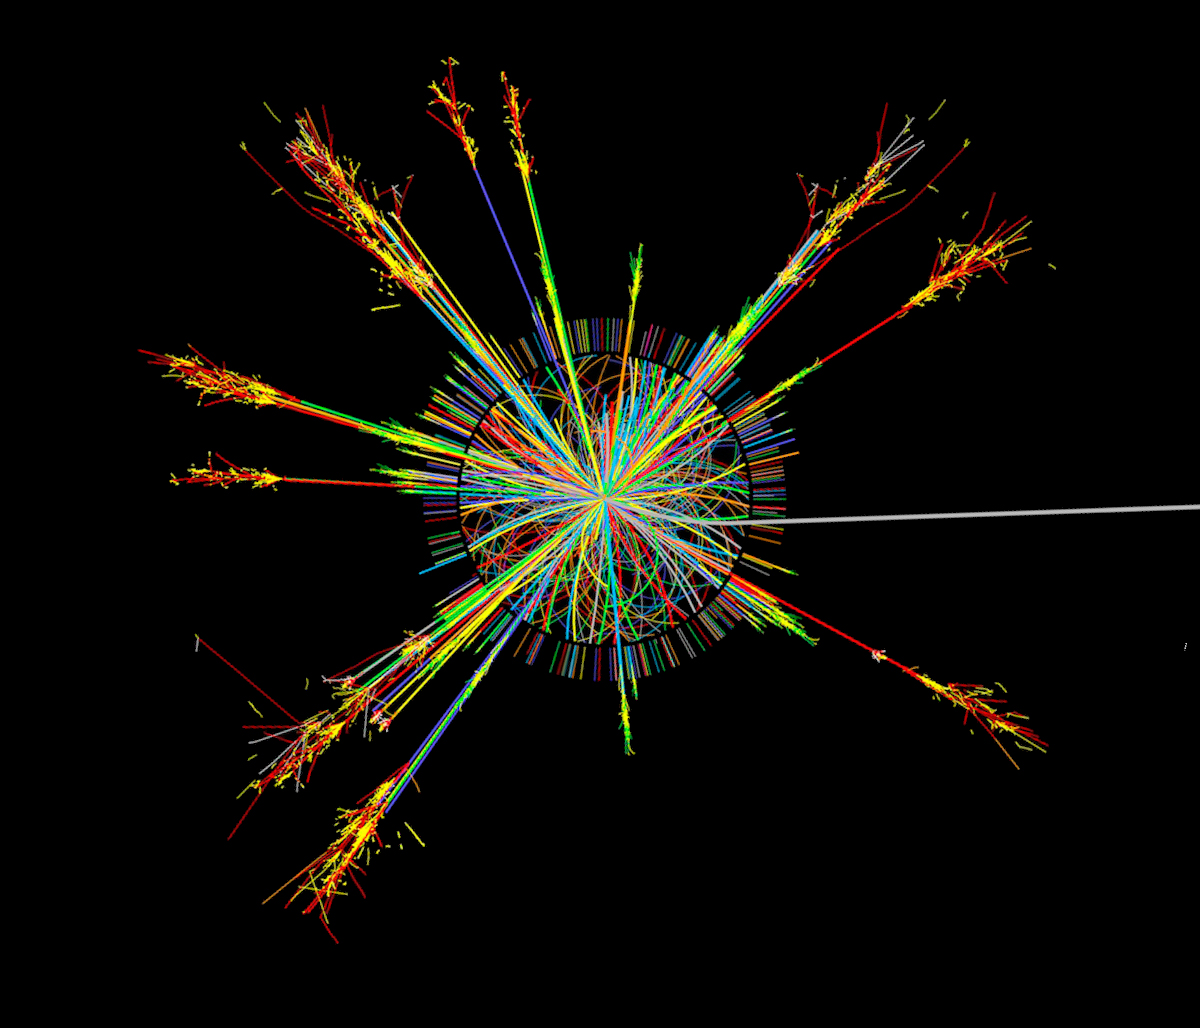
\includegraphics[width=.85\paperwidth]
                        {title/jettitleimage}}
};
\framenode[100pt]{image}
\end{tikzpicture}

% Author
\textcolor{amber}{\subtitlefont{Samuel Alipour-fard}}
\end{center}

\clearpage
\restoregeometry
\setcounter{page}{1}



%%%%%%%%%%%%%%%%%%%%%%%%%%
% Front Matter:
%%%%%%%%%%%%%%%%%%%%%%%%%%

% ---------------------------------
% Dedication
% ---------------------------------

{\clearpage           % we want a new page
   \thispagestyle{empty}% no header and footer
   \vspace*{\stretch{1}}% some space at the top
   \begin{center}
       {\itshape To the student}
       \vfill\vfill\vfill
       \text{This thesis is based on a true story.}
   \end{center}
}
{\par % end the paragraph
   \vspace{\stretch{3}} % space at bottom is three times that at the top
   \clearpage           % finish off the page
}


% ---------------------------------
% Other front matter
% ---------------------------------
\begin{center}
    ~
    \vspace{50pt}

    {\LARGE \textbf{Particles Inside Particles:} }

    \vspace{10pt}

    {\LARGE \textbf{The Flow of Energy in Quarks, Gluons, and Jets} }

    \Large

    \vspace{30pt}

    by

    \vspace{25pt}

    Samuel Alipour-fard

    \vspace{40pt}
    % \hrule
    \vspace{40pt}

    Submitted to the Department of Physics in partial fulfillment of the requirements for the degree of

    \vspace{20pt}

    DOCTOR OF PHILOSOPHY

    \vspace{15pt}

    at the

    \vspace{15pt}

    MASSACHUSETTS INSTITUTE OF TECHNOLOGY

    \vspace{20pt}

    May 2025


    \vspace{40pt}
    % \hrule
    \vspace{40pt}

    \copyright{} 2025 Samuel Alipour-fard. All rights reserved.

\end{center}


\newpage

% Sample thesis committee page for mitthesis.cls
% Version 1.02, 2025/01/28
%
% This page is not required by the MIT Libraries, but some departments require it.
%
% Insert between title page and abstract page.
% Format this page in any way that you like.
% Add supervisor titles, degrees, and departments as appropriate.

%%%%% FORMATTING COMMANDS %%%%%%%%%%%%%%%%%%

%% Format title
\NewDocumentCommand\CommitteePageTitle{m}{
	% \vspace*{40pt}
	\IfPackageLoadedTF{microtype}
		{\textls*{\Large\textbf{\MakeUppercase{#1}}}}
		{{\Large\textbf{\MakeUppercase{#1}}}}%
	\pdfbookmark[0]{#1}{Committee}%
	% \vspace*{10pt}%
}
% \textls* produces additional letter separation (appropriate for capitalized display text),
% PROVIDED THAT \usepackage{microtype} has been loaded in the preamble.
% The extra space added is 100/1000 em (adjustable, see package documentation).

%% Format committee member subheadings
\NewDocumentCommand\Role{m}{
	\vspace*{25pt}
	\IfPackageLoadedTF{microtype}
		{\textls*{\large{\textsc{#1}}}}
		{{\large\textsc{#1}}}%
	\vspace*{10pt}%
}

\newcommand{\hruledotted}[2]{
\begin{flushleft}
    {\Large #1 by} \hbox to #2{\leaders\hbox to 5pt{\hss . \hss}\hfil}
\end{flushleft}
}
%%%%%%%%%%%%%%%%%%%%%%%%%%%%%%%%%%%%%%%%%%%%%

\begin{flushright}

\CommitteePageTitle{Thesis committee}

\Role{Thesis Supervisor}

\vspace{10pt}

\textbf{Jesse Thaler}
\vspace{-18pt}
\hruledotted{Certified}{9.7cm}
\vspace{-5pt}
{\itshape
Professor of Physics
\\
MIT Center for Theoretical Physics
}%
% \\
% Director of the NSF Institute for Artificial Intelligence and Fundamental Interactions
\end{flushright}

\begin{flushright}
\Role{Thesis Readers}

\vspace{10pt}

\textbf{Iain Stewart}
\vspace{-18pt}
\hruledotted{Certified}{9.7cm}
\vspace{-5pt}
{\itshape
Professor of Physics
\\
MIT Center for Theoretical Physics
\\[18pt]
}
\end{flushright}

\vspace{10pt}

\begin{flushright}
\textbf{Christoph Paus}
\vspace{-18pt}
\hruledotted{Certified}{9.0cm}
\vspace{-5pt}
{\itshape
Professor of Physics
\\
MIT Laboratory for Nuclear Science
}%
\end{flushright}
% \\
% Co-lead for the CMS Experiment search for the Higgs Boson


\vspace{20pt}
\hrule
\vspace{-5pt}


\begin{flushright}
\Role{Author}

\vspace{10pt}

\textbf{Samuel Alipour-fard}
\vspace{-18pt}
\hruledotted{Submitted}{7.8cm}
\vspace{-5pt}
{\itshape
MIT Center for Theoretical Physics}
\end{flushright}

\begin{flushright}
\Role{Department Head}

\vspace{10pt}

\textbf{Deepto Chakrabarty}
\vspace{-18pt}
\hruledotted{Accepted}{8.0cm}
\vspace{-5pt}
{\itshape
Professor of Physics
\\
Kavli Institute for Astrophysics and Space Research
}
\end{flushright}

\cleardoublepage


\newpage

%   Reduce the margin of the summary:
\def\changemargin#1#2{\list{}{\rightmargin#2\leftmargin#1}\item[]}
\let\endchangemargin=\endlist

%   Generate the environment for the abstract:
\newcommand\summaryname{Abstract}
\newenvironment{Abstract}%
{%
    % \small%
    \begin{center}%
        \bfseries{\summaryname}%
    \end{center}%
}

\begin{Abstract}
\begin{changemargin}{0.5cm}{0.5cm}
This thesis presents the author's work in developing probes of the inner structure of jets in high-energy particle collisions.
%
We begin by introducing QCD and the scattering of partons (quarks and gluons), discussing jets as theoretical and experimental proxies for partonic physics, and presenting the partonic cascade model of jet formation and jet substructure.
%
Noting the ubiquitous presence of low-energy pollution in particle collision events, in the forms of hadronization, detector effects, the underlying event (UE), and pileup (PU), we then move towards the modern research area of developing pollution-insensitive probes of jet substructure.
%
Pollution-insensitive features of jet substructure are often accessed theoretically either through jet grooming or energy-weighted correlation functions.
%
We present the basics of the modern theory of jet grooming as well as the work of the author in developing the \textsc{Piranha} paradigm for \textit{continuous} jet grooming, introduced by the author in \Reff{Alipour-Fard:2023prj}, and explore the formal and phenomenological benefits of continuous grooming techniques as pollution-insensitive probes of jet substructure.
%
We also introduce the basics of the simplest energy-weighted correlation function -- the energy-energy correlator (EEC), which probes angular correlations between particle pairs -- and discuss its many-particle analogues.
%
We focus on the efficient and visually intuitive projected and resolved energy correlators introduced by the author in \Reff{Alipour-fard:2024szj}, which provide computationally-realistic, pollution-insensitive probes of angular many-body correlations in QCD jets.
%
Finally, we exposit the generic theory of energy-weighted observable correlations (EWOCs), introduced by the author in \Reff{Alipour-fard:2025dvp}, which utilizes the energy weighting of the EEC to provide pollution-insensitive probes of non-angular correlations within jets.
\end{changemargin}
\end{Abstract}


\newpage

\section*{Acknowledgements}
% \markboth{Acknowledgements}{Acknowledgements}

\epigraph{``Understanding is love's other name.''}{Thich Nhat Hanh}
\vspace{-20pt}
\epigraph{``We're philosophers. We think, therefore we am.''}{\textit{Small Gods}, Terry Pratchett}
\vspace{-20pt}
\epigraph{Films live or die on their casting.}{\href{https://youtu.be/W5bB7-jg_4M?list=PLomTW5B3fAMXJsqE_HDiMpdOdcfAk_Lqc&t=146}{Peter Jackson}}

I try as often as I can to remember that we live on a miraculous, miniscule blue dot floating in a vast expanse of emptiness, with scant resources and an incredible story.
%
It is the joy of my life to be part of the humanity sector of team earth.

\vspace{10pt}
\hrule

\begin{center}
Like most of the humanity sector, I am nothing without my mentors.
\end{center}


My first acknowledgements are to my tireless advisor, Jesse Thaler.
%
Thank you for taking me under your vast wing.
%
I have been very lucky to learn from your mastery over every aspect of the scientific process.
%
I have never seen someone do and change so much in the world in such a short time.



My second acknowledgments are to my parents, without whom I would surely not be here.
%
My mother taught me, through her shining example, the values of kindness, openness, acceptance, and sharp awareness and fighting spirit.
%
My father taught me by lack of example the importance of \glslink{jet-grooming}{grooming}, discussed further in \Chap{grooming}.
%
He also gave me the gifts of critical thinking, his jeans, and uncountable priceless lessons, experiences, and memories.



Tengiz Bibilashvili, my academic advisor during my time as an undergraduate at the University of California, Santa Barbara (UCSB), is one of the sharpest, kindest, brightest, and most generous human beings I have ever met.
%
I am grateful every day that I was lucky enough to experience his teaching.



Nathaniel Craig, my research advisor at UCSB, is a powerhouse of intellect, creativity, and pedagogy;
%
I benefited deeply from his dedication to mentorship and patience, and would have been lost on the tip of the iceberg of quantum field theory without his guidance (though, as he would always say with a smile, he was ``just doing his job'').



There is not enough I can say about the mentorship of Seth Koren.
%
Seth is incredibly empathetic and creative, and a brilliant teacher.
%
Seth is, to me, a quintessential human being:
%
a philosopher, clever and kind, who accepts nothing but the truth.



Finally, Wouter Waalejwin, who I met in the fourth year of my PhD, has been an incredibly patient mentor and a valuable resource for me in learning the ins and outs of quantum chromodynamics.
%
His presence is felt in many subtle ways throughout this thesis.
%
I can see his gentle, knowing smile even now.



I would also like to thank Iain Stewart and Christoph Paus.
%
They are members of my thesis committee, and I am grateful for their time and effort on my behalf, but I am most grateful for the environment they created at MIT through their presence.
%
They always had a warm comment to make or a laugh to share.
%
I knew I could always go to Iain with any question or concern and receive a listening ear and some sound advice.
%
I knew that I could always share a joke and a lighthearted chuckle with Christoph.


On the topic of environment, I would finally like to thank Daniel Harlow, who always had time to give a smile, kind words, and guidance in physics or beyond.


\vspace{12pt}
\hrule
\vspace{12pt}


My sisters, Christina Nazmi-Williams and Mehrnoush Minor (\textit{in alphabetical order}), are my role models and favorite people.
%
It is thanks to their hard work and sacrifices on my behalf that I have been able to live such a clear and irresponsible life.
%
I am so lucky to be in their family.
%
Thomas Minor, my brother-in-law, is another favorite.
%
I aspire to someday be like Tom:
%
brilliant and humble, quietly aware and listening more than speaking, kind and gentle with a troublemaking streak.
%
My nephews and niece -- Ethan and Mason Williams, and Alex and Amelia Minor -- are bundles of joy and diamonds of my life.



My godparents Pieter and Martha van der Mersch, and my godsiblings Anna and Stephan, have provided my life with incredible warmth, amazing memories, and more empathy and useful guidance than I could have ever hoped for.



I also have the best siblings I could ever hope not to be related to.
%
Noah Mihelic (with credit and gratitude to my adopted family: Adrienne, Mark, and Josh Mihelic), who I knew before I had memories, has given me clarity, critical reasoning, incredible companionship, and many magical adventures.
%
David Rower (with credit and gratitude to my adopted family: Rachel Goldberg, Tobin Rower, Nathan Rower, and Lamia Ateshian) is funny, creative, and intelligent beyond words.
%
He has taught me countless invaluable lessons about being a clear and kind human being.
%
To say that his infectious positivity has changed my life is an understatement.
%
J Rogers is always, \textit{always} there when I need them, and whose incredible clarity and kindness is something I aspire to and benefit from every day.
%
Neeraj Tata, my hobbit-in-crime, has an incredible (and intentionally trained) ability of using sharp awareness and tolerance of all things to see what is really important in this life.


My academic siblings have also been important parts of my journey, and have taught me and been with me through both trials and tribulations.
%
Sean Benevedes, who I have known since my time at UCSB, carries with him an intelligence, humor, and empathy that make world a measurably better place.
%
I have also benefited from many useful conversations with Rikab Gambhir, whose funny jokes, intelligence, and unimpeachable sense of academic adventure have made my experience at MIT much more interesting.
%
Last but not least, Cari Cesarotti is a hilarious, high-powered, creative scientist who I love to watch playing the game of science and winning.



\vspace{10pt}
\hrule
\vspace{10pt}



The remainder of my acknowledgments are mostly chronological, and no less heartfelt.


I want to thank some of my first and most long lasting friends:
%
Liam Bradley, Daniel Kreizberg, Nate Gardner, Kyreija Lamothe, Vince Fleming, Ryan Croy.
%
Also there to support me during many formative moments were Rose Gordon, Erin Neitzel, Jason Georgis, Johannes Klein, and especially Nicholas Maguid.



More of my academic family from UCSB who have had an incredible positive influence on my life are James Ehrets (I have learned and gained so much from his openness and adventurousness, empathy, and many long conversations), Nicholas O'Dea (who perhaps belongs in my ``mentor'' section: he has shaped my entire attitude towards learning and rigor), David Newsom (he knows the many odd and memorable adventures we have shared together -- what an incredible and interesting life), Jasmin Kwak (who is an unshakeable source of support whenever I need her), Ben Siegel (whose gentle kindness I always aspire to), Dolev Bluvstein (who is a damn superhuman -- I don't know how he does it, but I feel so lucky to learn from his incredible positivity and brilliant approach to all of life), Anoop Praturu, Ryan Stuart, and Marvin Qi.
%
My b-boy crew, including Kai Goh, Eugene Ma, Brandon Louie, and Alvin Ong have given me many adventures as well, along with companionship, growth, a beautiful and positive environment for my studies, and the incredible gift of \emph{art}.
%
Last, and perhaps most important, is Yurim Lee, who gave me so much kindness, supported me through


At MIT, I was lucky enough to meet even more incredible and brilliant people.
%
I'm very grateful to Zhiquan Sun, who taught me among many wonderful lessons that a happy life means eating well.
%
Another close friend is Christopher McNally, who is open to anything, saved my life in the wilderness on one occasion, and saved my spirit in and out of the halls of MIT many more.
%
Some of my first friends at MIT were Atakan Firat (a tireless dynamo of intellect and creativity who never backs down from a fight), Ouail Kitouni (humble beyond belief, whose openness and kindness are only emphasized by his incredible knowledge, curiosity, and problem-solving ability), Shankar Balasubramanian (a pure genius, plain and simple, always with time to teach, share a problem, or give advice), Margarita Davydova (a kind, creative, brilliant theorist who makes science as beautiful as art), Ali Ghorashi (always with support and empathy to share), and Anjie Gao (who taught me, among other things, the wisdom that ``nothing is trivial'').
%
Though it took one more semester, I soon met Patrick Oare, Wenzer Qin, Artur Avkadiev -- my moral support group -- who have since been my people:
%
my confidants, my comrades-in-arms, my rocks.
%
Nick Kamp and Caolan John also deserve a special mention here;
%
they bring positivity and curiosity into every room, and every room is better for their presence.
%
Nathan Everett (my platonic soul mate) and Lubah Lerner (his soul mate) have also been close friends and wonderful sources of joy and support.
%
I have been lucky enough to learn from and share time with Dimitra Pefkou, \r{A}smund Folkestad, Gregory Ridgway, Joshua Lin, Yitian Sun, Sarah Geller, Jamison Sloan, Robert Jones, Manu Srivastava, and Ankita Budhraja.
%
I especially want to thank Lisa Yang, whose constant drive for self-improvement is continually inspiring.


The entirety of the Engineering Quantum Systems (EQuS) ``chill team'' deserves a special mention for the joy they have brought to my life:
%
Sarah Muschinske, Miguel and Lean\'or Moreira, Jorge Marques, and Andreia Allen -- and also to Will Oliver, whose incredible positive and guiding influence has brought these wonderful, brilliant people together.  % TODO: fix Leanor if necessary
%
David Rower, Lamia Ateshian, and Dolev Bluvstein deserve more thanks here as well, and Marcin Kalinowski should be thanked three times (once for his wonderful personality, twice for his incredible science, and three times for his enormous muscles, which count as another person on their own).


Finally, I remember Jasper Pont, whose ringing laugh and free spirit still float through the world.

\vspace{12pt}
\hrule

\begin{center}
    \textit{Ashes to ashes, dust to dust.}
\end{center}


\newpage

\section*{Preface}
% \markboth{Preface}{Preface}

\epigraph{Question everything at least once.}{Mansour Alipour-fard}

\epigraph{You earn your right to speculate depending on how much work you do.}{Barton Zwiebach}


The nominal goal of this thesis is to present my research from my time in graduate school.

Another goal I have is that, in a couple of (albeit concerted) weeks, you can master what took my six years to learn (to the extent that I have mastered it)!
%
First, and most importantly, please remember that problems are a \textit{shortcut} to understanding, not ``something extra''.
%
At least, good problems are.
%
I've tried to select and invent some good problems for you%
\footnote{
    And if you have any comments or qualms regarding any of them, you should feel free to email me.
}
%
that I hope are representative of
\begin{itemize}
    \item
        the story or ``flavor'' of the material;

    \item
        the physical concepts, and the intuition I have for the material;

    \item
        the mathematics required to do some realistic (albeit simple) computations.
\end{itemize}
%
From what I've seen and read, active learning is the quickest and only way.
%
Don't forget!

Before we begin the thesis, I will add some clarifying comments regarding both goals.
%
First, my main contributions presented in this thesis are
\begin{itemize}
    \item
        The introduction of the \PIRANHA{} paradigm for continuous grooming, with Eric Metodiev, Patrick Komiske, and Jesse Thaler.
        %
        This research was presented in \ul{Pileup and Infrared Radiation Annihilation (PIRANHA): A Paradigm for Continuous Jet Grooming} \cite{Alipour-Fard:2023prj}.
        %
        For \PIRANHA{}, see especially \Secss{piranha}{sd_discont}{grooming-pheno};

    \item
        The development of new, efficient, and visually intuitive higher-point energy correlators -- both \emph{projected} (PENCs) and \emph{resolved} (RENCs) with Ankita Budhraja, Wouter Waalejwin, and Jesse Thaler.
        %
        This research was presented in \ul{New Angles on Energy Correlators} \cite{Alipour-fard:2024szj}.
        %
        For PENCs and RENCs, see \Sec{new-angles};

    \item
        The initiation of the study of general energy-weighted correlations, called Energy Weighted Observable Correlations (EWOCs), that are not restricted to angular correlations (e.g. as in the case of PENCs and RENCs).
        %
        This research was presented in \ul{Energy Correlators Beyond Angles} \cite{Alipour-fard:2025dvp}.
        %
        For EWOCs, see especially \Sec{ewocs}.
\end{itemize}

Second, since I attempt to provide especially clear and step-by-step derivations which highlight at least my own assumptions, several of the derivations presented in this thesis, even of fundamental concepts, are original.
%
Though their conclusions are backed by history, I invoke the uncertainty principle, and advise you to watch closely for their \emph{correctness}.
%
I hope to have given enough detail to make this possible, and I encourage you to email me if I have not.
%
The framework I derive has definite limitations, including (but not limited to):
\begin{itemize}
    \item
        There is no formal discussion of the ``accuracy'' of our computations -- we simply take the soft- and collinear-limits as often as we must to make progress;

    \item
        There is no systematic regularization of infrared divergences;
\end{itemize}
I would be delighted to hear if you know of any places where my discussion is lacking.

Finally, in addition to the several texts that appear in my citations below, another under-celebrated text on \glslink{qcd}{quantum chromodynamics} is \underline{Applications of Perturbative QCD}, by Richard D. Field \cite{Field:1989uq}, which pays incredible attention to detail in the presentation of calculations.
%
Of course, it would be a shame to access this book quickly, easily, and for free using \url{libgen.is}, so I will mention that it is also available (at time of writing) at \href{https://www.desy.de/~jung/qcd_and_mc_2009-2010/R.Field-Applications-of-pQCD.pdf}{\texttt{this desy.de link}}.

\begin{center}
Good luck.
\end{center}


\newpage

\section*{Prerequisites}
% \markboth{Prerequisites}{Prerequisites}

\epigraph{``You earn your right to speculate depending on how much work you do.''}{Barton Zweibach}

In order to understand the technical details of the material in this thesis, I expect that the following prerequisites are necessary (if you can understand them without these prerequisites, great work!):
\begin{itemize}
    \item
        A course in quantum field theory, or at least an understanding of quantum mechanics and the basics of particle physics.

    \item

\end{itemize}

In addition, I expect that you should probably be able to understand the following pieces of physics:
\begin{itemize}
    \item
        The strong coupling \(\alpha_s(\mu)\) obeys the \vocab{renormalization group equation}
        \begin{equation}
        \mu \frac{d}{d\mu} \alpha_s(\mu) = \beta(\alpha_s(\mu))
        =
        - \sum_{n=0}^\infty \beta_n
        {\left(\frac{\alpha_s(\mu)}{4\pi}\right)}^{n+2},
        \end{equation}
        \sam{check} with the first \vocab{beta function coefficient}
        \begin{equation}
            \beta_0
            =
            \frac{1}{4\pi}\le(
                \frac{11}{3} C_A - \frac{4}{3} T_F n_f
            \ri)
            ,
        \end{equation}
        taking an important role at one-loop and in the studies in this thesis.

    \item
        The running of the strong coupling leads to a special scale by \vocab{dimensional transmutation}:
        %
        given the coupling at some scale \(\mu\), the form of the beta function indicates that the coupling becomes infinite at a scale we call \(\LambdaQCD\).
        %
        Ignoring the effects of the beta-function coefficients other than \(\beta_0\), we have
        \begin{equation}
            \LambdaQCD = \mu \exp\left(-\frac{1}{2\beta_0 \alpha_s(\mu)}\right).
        \end{equation}
        \sam{This was just written by copilot -- double check in terms of these definitions.}
\end{itemize}



In addition, since we are lucky enough to live in the age of free internet resources, I will mention the following incredible texts:

\textbf{Basics of Quantum Field Theory:}
\begin{itemize}
    \item
        \underline{Book name}, by \sam{author}

        This book \sam{does ...}

        Available at \sam{place/url}
\end{itemize}


\textbf{Specific References for QCD:}
\begin{itemize}
    \item
        \underline{Applications of Perturbative QCD}, by Richard D. Field;

        This book \sam{does ...}

        Of course, it would be a shame to access this book quickly, easily, and for free using \url{libgen.is}, so I will mention that it is also available (at time of writing) at \href{https://www.desy.de/~jung/qcd_and_mc_2009-2010/R.Field-Applications-of-pQCD.pdf}{this desy.de link}.
\end{itemize}


\newpage

% =====================================
\section*{Notation and Terminology}
% =====================================
% \markboth{Notation and Terminology}{Notation and Terminology}


\epigraph{If you think this Universe is bad, you should see some of the others.}{Philip K. Dick}

Here is some common notation used throughout this thesis.
\begin{itemize}
    \item
        \(A := B\) means ``\(A\) is defined to mean \(B\)'', as does \(B =: A\);

    \item
        For simplicity, I set the physical constants \(\hbar = c = 1\) in all printed equations;

    \item
        We make the unfortunate choice to use the ``mostly-minus'' metric, \(g^{\mu\nu} = \text{diag}\le(+,\,-,\,-,\,-\ri)\), such that \(\acomm{\gamma^\mu}{\gamma^\nu} = 2 g^{\mu\nu}\), and with the saving grace that we can write \(p^2 = m^2\).

    \item
        We will use the symbol \(z_i\) to denote the energy fraction particle \(i\) relative to a ``parent'' of any type, such as a pair of particles, a jet, or an entire event (which of these should be clear based on context):
        \begin{align}
            z_i
            \eqdelta
            \frac{E_i}{E_\text{tot}}
            \,.
        \end{align}


    \item
        We will also use the following standard definitions:%
        \footnote{
            We are leaving out the term \(-\epsilon \alpha_s\) that appears in \(d=4-2\epsilon\) dimensions when defining \(\alpha_s\) to be dimensionless.
            %
            The extra factor of two in the beta function vanishes if one defines the beta function instead to be the derivative of \(\alpha_s\) relative to \(\ln\mu^2\), or if it is written in terms of \(g_s\):
            %
            \(\dd g_s / \dd\ln_\mu = - g_s \sum_n \beta_n \le(\alpha_s/4\pi\ri)^{n+1}\).
        }
        \begin{subequations}
        \label{eq:qcd_coupling}
        \begin{align}
            \label{eq:as_defn}
            \alpha_s = \frac{g^2_s}{4\pi}
            \,,&
            \qquad\quad
            \as = \frac{\alpha_s}{4\pi}
            \,,
            \\
            \label{eq:beta_fn_defn}
            \beta(\alpha_s)
            :=
            \frac{\dd}{\dd\log\mu}\alpha_s&(\mu)
            =
            -2 \, \alpha_s
            \sum_{n=0}^\infty
            \beta_n \le(\frac{\alpha_s}{4\pi}\ri)^{n+1}
            \,.
        \end{align}
        At one loop (i.e. ignoring \(\beta_m\) for \(m \geq 1\)),
        \begin{align}
            \label{eq:alphas_1loop}
            \alpha_s^\text{(1-loop)}(\mu)
            &=
            \frac{\alpha_s(Q)}{1 + \alpha_s(Q) \beta_0 \log(\mu/Q)/2\pi}
            \,.
        \end{align}
        where
        \begin{align}
            \beta_0 = \frac{11}{3}\,C_A - \frac{4}{3}\,T_f N_f
        \end{align}
        \end{subequations}
        is the leading coefficient of the QCD beta function, \(N_f\) denotes the number of effectively massless quark flavors (\(N_f = 5\) in this thesis), \(Q\) indicates a reference scale (such as the energy scale of a hard process), and
        \begin{align}
        \label{eq:group_theory}
            C_F = \frac{N_c^2 - 1}{2N_c}
            \xrightarrow[]{\text{QCD}}
            \frac{4}{3}
            \,,
            \qquad
            C_A = N_c
            \xrightarrow[]{\text{QCD}}
            3
            \,,
            \qquad
            T_F = \frac{1}{2}
            \,,
        \end{align}
        denote the quadratic Casimir for the fundamental representation of \(SU(N_c)\), the quadratic Casimir for the adjoint representation, and the Dynkin index of the fundamental representation, respectively.
        %
        The expressions of \Eq{group_theory} are often referred to collectively as \textit{group theory factors}.
        %
        For QCD, \(N_c = 3\), \(C_F = 4/3\), and \(C_A = 3\), giving \(\beta_0 = 11 - 2 N_f / 3\,.\)


    \item
        The \glslink{splittingfn}{Dokshitzer-Gribov-Lipatov-Altarelli-Parisi (DGLAP) splitting functions}, computed in \Sec{splitting-functions} and related to the \glslink{dglapeqn}{DGLAP equation} in \Sec{p2p-fragmentation}, are sometimes written in the \emph{exclusive} form \(P_{i\,j \leftarrow \ell}(z)\), with a probabilistic interpretation related to the probability of a parton of type \(\ell\) to split into partons of type \(i\), carrying an energy fraction \(z = z_i = E_i / E_\ell\), and type \(j\), carrying an energy fraction of \(z_j = 1-z\).
        %
        The \emph{inclusive} (meaning ``including a sum over some final state information'') DGLAP splitting functions are defined by
        \begin{align}
            \sum_{k'} P_{i\,k' \leftarrow \ell}(z) =: p_{i\leftarrow \ell}(z)
            \,.
        \end{align}


    \item
        The Mellin transform of a function \(f(x)\) with support on the interval \((0,1)\) (as in all concrete applications in this work) is
        \begin{align}
            \mathcal{M}[f](s)
            \eqdelta
            \int_0^1 \,\frac{\dd x}{x}\, x^{s-1} \, f(x)
            =
            \hat f(s)
            \,.
        \end{align}

\end{itemize}


Furthermore, we will assume
\begin{itemize}
    \item
    That all partons are massless other than the top quark (whose effects we will mostly ignore);

    \item
    That we may ignore electroweak effects (i.e. perform calculations without the \(W\) and \(Z\) bosons).
\end{itemize}


\clearpage

% ---------------------------------
% Table of Contents
% ---------------------------------
\begingroup

\let\MakeUppercase=\relax  % for header

\begingroup

\titleformat{\chapter}[display]
{\normalfont\huge\bfseries\sffamily}{}{25pt}{\chaptitlenonumber}
\titlespacing{\chapter}{0pt}{-15pt}{25.5pt}

\tableofcontents{
    \fancyhead[LO]{\slshape\contentsname}
    \fancyhead[RE]{\slshape\contentsname}
}

\endgroup

\clearpage{}

% ---------------------------------
% List of Figures/Tables/Problems
% ---------------------------------
\listoffigures{
    \fancyhead[RE]{\listfigurename}
    \fancyhead[LO]{\listfigurename}
}

\clearpage{}

\listoftables{
    \fancyhead[RE]{\listtablename}
    \fancyhead[LO]{\listtablename}
}

% TOGGLE: list of problems
% DEBUG: no page breaks in listsofX

% \listofproblems{
%     \fancyhead[LE]{\listproblemname}
% }

\endgroup
\fi  % ifshowfrontmatter


% %%%%%%%%%%%%%%%%%%%%%%%%%%%%%%%%%%%%
% Chapters:
% %%%%%%%%%%%%%%%%%%%%%%%%%%%%%%%%%%%%
\ifshowmainmatter

\mainmatter{}

% Chapter titles with numbers
\titleformat{\chapter}[display]
{\normalfont\huge\bfseries\sffamily}{}{25pt}{\chaptitle}
\titlespacing{\chapter}{0pt}{-15pt}{25.5pt}


% ==============================================
\chapter[Quantum Chromodynamics (QCD): A Picture Book]{Quantum Chromodynamics:\\A Picture Book}
\markboth{\small \textsc{Chapter \thechapter}: \bf QCD: A Picture Book}{}

\label{chap:picturebook}

\epigraph{Never trust an atom: they make up everything.}{An atom}

\epigraph{There are more things in Heaven and Earth, Horatio, than are dreamt of in your philosophy.}{Shakespeare, \underline{Hamlet}}


70 years ago, humanity discovered new particles that nobody expected.
%
Dozens of them.
%
After the conceptualization of molecules in the 19\th{} century, atoms in the 20\th{} century, and the even smaller protons, neutrons, electrons, muons, and neutrinos, you may have thought we had seen the building blocks of everything under the sun.
%
But we hadn't.

The discovery of the zoo of new particles -- what we called the \(\Delta\), the \(K^*\), the \(\rho\), and scores of others -- showed us that everything we knew was not enough.
%
The next 20 years saw a bedlam of earnest confusion, controversy, and adventure in the field of particle physics, as humanity desperately strove to understand the moves of over one hundred new chess pieces.
%
The all-encompassing framework of \gls{qft}, the great unifying language of modern physics, faltered.
%
By the 1960s, it teetered on the edge of irrelevance -- mocked, dismissed, almost forgotten.
%
Nearly consigned to oblivion, \gls{qft} seemed to raggedly breathe its last.

\textit{Then, it came roaring out of its deathbed in triumph.}

Hidden in the chaos of hundreds of numbers -- masses, charges, decay rates -- lay a deep order glimpsed by Gell-mann \cite{Gell-Mann:1964ewy} and Zweig \cite{Zweig:1964ruk,Zweig:1964jf} in their quark model, and in the geometric theory of Yang and Mills \cite{Yang:1954ek}, which forged together into the theory of \gls{qcd}.
%
In radical defiance of the theorists of the previous generation, Politzer \cite{Politzer:1973fx} and Gross and Wilczek \cite{Gross:1973ju} discovered that QCD was one of the only quantum field theories invulnerable to the disparagements of their predecessors.
%
We had obtained a theory of the strong force;
%
a theory that overcame decades of confusion, and explained our unexpected observation of dozens of new particles.

\textit{The mystery of the particle zoo was the manifestation of the symmetries of QCD.}


\vspace{1.5cm}
\hrule
\begingroup

\setlength \epigraphwidth {\textwidth}
\setlength \epigraphrule {0pt}
\renewcommand {\epigraphflush} {center}
\renewcommand {\sourceflush} {center}

\epigraph{
        When you ask what are electrons and protons I ought to answer that this question is not a profitable one to ask and does not really have a meaning.
    %
    The important thing about electrons and protons is not what they are but how they behave, how they move.
    %
    I can describe the situation by comparing it to the game of chess.
    %
    In chess, we have various chessmen [sic], kings, knights, pawns and so on.
    %
    If you ask what a chessman is, the answer would be that it is a piece of wood, or a piece of ivory, or perhaps just a sign written on paper, or anything whatever.
    %
    It does not matter.
    %
    Each chessman has a characteristic way of moving and this is all that matters about it.
    %
    The whole game of chess follows from this way of moving the various chessmen.
}{---Paul Adrien Maurice Dirac}

\endgroup

\vspace{0.2cm}
\hrule
\vspace{1.5cm}


As we explored our universe, it slowly became clear that QCD described the inner lives of many of the particles we saw.
%
Just as Rutherford beheld the astounding result that atoms had an inner structure formed by protons and neutrons in the early 20\th{} century, the experiments of the late 20\th{} century showed that protons and neutrons were themselves made of more fundamental pieces.

Feynman named the new chess pieces partons, Gell-mann named them quarks and gluons, and we began to understand that they composed protons, neutrons, and the dozens of new particles of the particle zoo.
%
But we saw something even more curious.
%
When we tried to produce quarks in particle collisions, evidence began to suggest that \textit{they themselves were composed of quarks}.
%
The experimental data matched the prediction that a single energetic quark or gluon produced in a particle collision underwent a dramatic fragmentation into many more partons.
%
In fact, the theory of QCD seemed to suggest that a single quark or gluon contained an \textit{infinite number of partons within}.

Luckily, Sterman and Weinberg discovered a way around the divergences of QCD \cite{Sterman:1977wj};
%
they predicted that the chess pieces of QCD at high energies, not unlike the water droplets spraying from a high pressure hose, should shower into \vocab{jets} each potentially containing dozens of particles or more.
%
The jets they predicted as proxies for the high energy quarks and gluons produced by colliding particles were soon measured \cite{Hanson:1975fe,Wiik:1979cq,Barber:1979yr,TASSO:1979zyf,PLUTO:1979dxn,JADE:1979rke,Ali:1979em,Hanson:1981em,Ali:2010tw}, and the explosion of experimental, phenomenological, and theoretical study of jets that followed solidified \gls{qcd} as our fundamental theory of the strong nuclear force.
%
It is not an exaggeration to say that the discovery of jets has been one of the most important developments in the history of our study of the natural world.

By studying the correlations of hadronic radiation within jets, we may probe their internal structure and gain even more information about the \gls{sm}, \gls{qcd}, and beyond.
%
However, the substructure of jets is difficult to predict, especially through the obfuscating haze of additional particles that accompany jets in the messy environment of particle collisions.
%
We must design jet substructure observables which are both experimentally meaningful and experimentally calculable, and are robust to the effects of the addition pollution produced by particle collisions.

\textit{To understand the most fundamental known building blocks of our universe, we must study the substructure of jets.}
%
\textbf{\textit{Designing robust probes to expose the fractal-like, inner life of jets through a haze of contaminating radiation is the subject of this thesis.}}



\begin{figure}[]
    {
        \hspace{-1.7cm}
        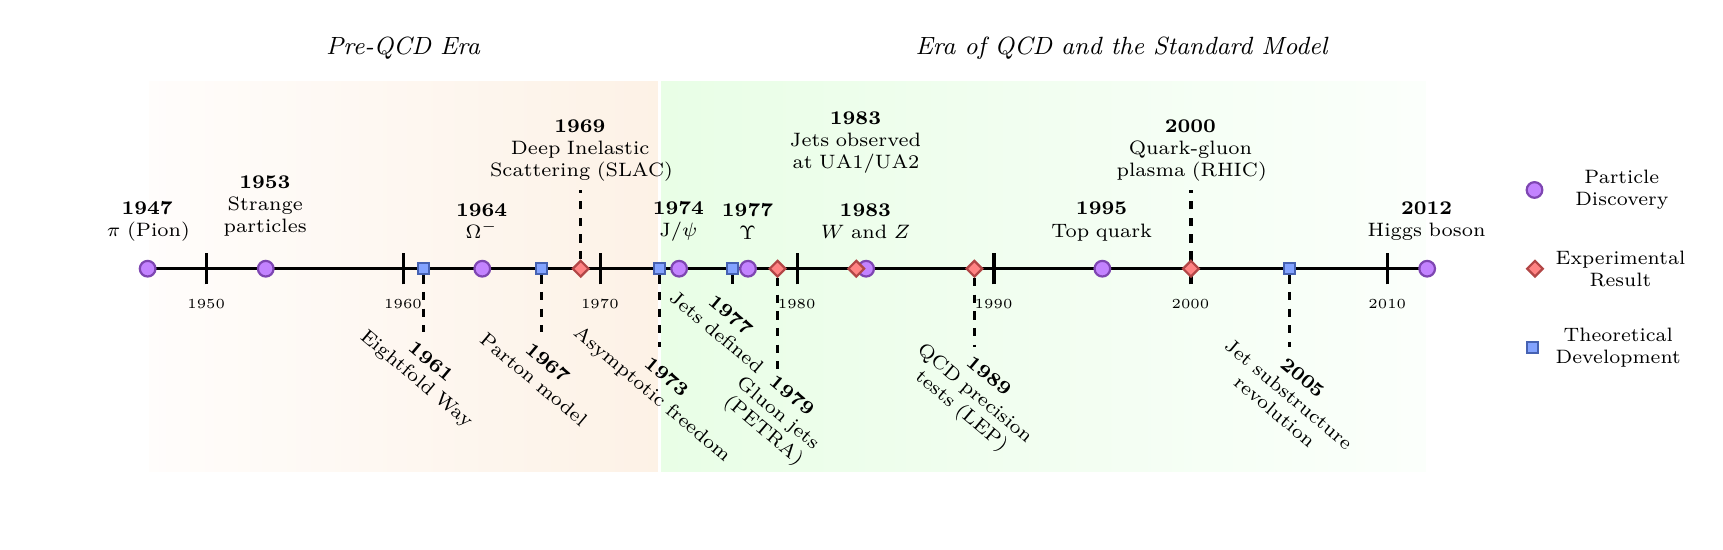
\begin{tikzpicture}[very thick]
    % Define coordinate transformation function
    \pgfmathsetmacro{\compressfactor}{1}
    \pgfmathsetmacro{\earlytransition}{1947}
    \pgfmathsetmacro{\moderntransition}{1973}

    \tikzset{
        my coords/.style={
            x={0.25cm},
            y={1cm},
        }
    }

    \begin{scope}[my coords]
        % Colors
        \definecolor{particleera}{RGB}{255,240,230}
        \definecolor{modernera}{RGB}{230,255,230}
        \definecolor{particledot}{RGB}{255,200,180}
        \definecolor{moderndot}{RGB}{180,255,180}
        \definecolor{particleoutline}{RGB}{255,140,100}
        \definecolor{modernoutline}{RGB}{50,180,50}

        % New colors for event types
        \definecolor{theorycol}{RGB}{100,140,255}
        \definecolor{experimentcol}{RGB}{255,100,100}
        \definecolor{particlecol}{RGB}{180,100,255}
        \definecolor{milestonecolor}{RGB}{100,40,120}

        % Styles
        \tikzset{
            experiment/.style={diamond, fill=experimentcol!80, draw=experimentcol!70!black, line width=0.8pt, inner sep=1.5pt},
            theory/.style={rectangle, fill=theorycol!80, draw=theorycol!70!black, line width=0.8pt, inner sep=2pt},
            particle/.style={circle, fill=particlecol!80, draw=particlecol!70!black, line width=0.8pt, inner sep=2pt},
            milestone/.style={particle}, % Now just using particle style for milestones
            exp label/.style={text width=2.8cm, align=center, font=\scriptsize},
            theory label/.style={text width=2.8cm, align=center, font=\scriptsize, rotate=-40},
            particle label/.style={text width=2.8cm, align=center, font=\scriptsize}
        }

        % Era backgrounds
        \fill[draw=white, left color=particleera!15, middle color=particleera, right color=particleera!90!modernera] (\earlytransition,2.4) rectangle (\moderntransition,-2.6);
        \fill[draw=white, left color=modernera!90!particleera, middle color=modernera, right color=modernera!15] (\moderntransition,2.4) rectangle (2012,-2.6);

        % Main timeline
        \draw[line width=1.2pt] (1947,0) -- (2012,0);

        % Era labels
        \node[font=\small\itshape] at (1960,2.8) {Pre-QCD Era};
        \node[font=\small\itshape] at (1996.5,2.8) {Era of QCD and the Standard Model};

        % Tick marks
        \foreach \year in {1950,1960,1970,1980,1990,2000,2010} {
            \draw (\year,-0.2) -- (\year,0.2);
            \node[below=0.05cm, font=\tiny] at (\year,-0.2) {\year};
        }

        % PARTICLE DISCOVERIES (placed at y=0 with vertical offsets and horizontal labels)

        % Pion (now a regular particle)
        \node[particle] (pion) at (1947,0) {};
        \node[particle label] at (1947,0.6) {\textbf{1947}\\$\pi$ (Pion)};

        % Strange particles
        \node[particle] (strange) at (1953,0) {};
        \node[particle label] at (1953,0.8) {\textbf{1953}\\Strange\\particles};

        % Omega-minus
        \node[particle] (omega) at (1964,0) {};
        \node[particle label] at (1964,0.6) {\textbf{1964}\\$\Omega^-$};

        % J/psi
        \node[particle] (jpsi) at (1974,0) {};
        \node[particle label] at (1974,0.6) {\textbf{1974}\\J/$\psi$};

        % Upsilon (added)
        \node[particle] (upsilon) at (1977.5,0) {};
        \node[particle label] at (1977.5,0.6) {\textbf{1977}\\$\Upsilon$};

        % W and Z bosons (added)
        \node[particle] (wz) at (1983.5,0) {};
        \node[particle label] at (1983.5,0.6) {\textbf{1983}\\$W$ and $Z$};

        % Top quark (added)
        \node[particle] (top) at (1995.5,0) {};
        \node[particle label] at (1995.5,0.6) {\textbf{1995}\\Top quark};

        % Higgs boson (now a regular particle)
        \node[particle] (higgs) at (2012,0) {};
        \node[particle label] at (2012,0.6) {\textbf{2012}\\Higgs boson};

        % EXPERIMENTAL EVENTS

        % DIS at SLAC (stays above)
        \node[experiment] (dis) at (1969,0) {};
        \draw[-, dashed] (dis) -- (1969,1.0);
        \node[exp label] at (1969,1.5) {\textbf{1969}\\Deep Inelastic\\Scattering (SLAC)};

        % Jets at UA1/UA2 (stays above)
        \node[experiment] (jets-exp) at (1983,0) {};
        \node[exp label] at (1983,1.6) {\textbf{1983}\\Jets observed\\at UA1/UA2};

        % Moved to bottom row
        % Gluon jets (MOVED to bottom)
        \node[experiment] (gluon) at (1979,0) {};
        \draw[-, dashed] (gluon) -- (1979,-1.3);
        \node[theory label] at (1979,-1.85) {\textbf{1979}\\Gluon jets\\(PETRA)};

        % LEP precision (MOVED to bottom)
        \node[experiment] (lep) at (1989,0) {};
        \draw[-, dashed] (lep) -- (1989,-1.0);
        \node[theory label] at (1989,-1.6) {\textbf{1989}\\QCD precision\\tests (LEP)};

        % Quark-gluon plasma (MOVED to bottom)
        \node[experiment] (qgp) at (2000,0) {};
        \draw[-, dashed] (qgp) -- (2000,1.0);
        \node[exp label] at (2000,1.5) {\textbf{2000}\\Quark-gluon\\plasma (RHIC)};

        % THEORETICAL EVENTS (below the line)

        % Eightfold Way
        \node[theory] (eightfold) at (1961,0) {};
        \draw[-, dashed] (eightfold) -- (1961,-0.8);
        \node[theory label] at (1961,-1.3) {\textbf{1961}\\Eightfold Way};

        % Parton model
        \node[theory] (parton) at (1967,0) {};
        \draw[-, dashed] (parton) -- (1967,-0.8);
        \node[theory label] at (1967,-1.3) {\textbf{1967}\\Parton model};

        % Asymptotic freedom
        \node[theory] (qcd) at (1973,0) {};
        \draw[-, dashed] (qcd) -- (1973,-1.0);
        \node[theory label] at (1973,-1.5) {\textbf{1973}\\Asymptotic freedom};

        % Jets defined
        \node[theory] (jets-theory) at (1976.7,0) {};
        \draw[-, dashed] (jets-theory) -- (1976.7,-0.2);
        \node[theory label] at (1976.3,-0.7) {\textbf{1977}\\Jets defined};

        % Jet substructure
        \node[theory] (substructure) at (2005,0) {};
        \draw[-, dashed] (substructure) -- (2005,-1.0);
        \node[theory label] at (2005,-1.6) {\textbf{2005}\\Jet substructure\\revolution};


        % Simplified Legend
        \begin{scope}[shift={(2017,0.0)}]
            \node[particle, anchor=west] at (0,1.0) {};
            \node[anchor=west, align=center, font=\scriptsize] at (2.0,1.0) {Particle\\Discovery};

            \node[experiment, anchor=west] at (0,0.0) {};
            \node[anchor=west, align=center, font=\scriptsize] at (1,0.0) {Experimental\\Result};

            \node[theory, anchor=west] at (0,-1.0) {};
            \node[anchor=west, align=center, font=\scriptsize] at (1,-1.0) {Theoretical\\Development};
        \end{scope}
    \end{scope}
\end{tikzpicture}

    }
    \caption[A rough timeline of the history of \gls{qcd}. \sam{incomplete}]
    {
        A rough timeline of the history of \gls{qcd}.
        %
        \sam{Not complete! Many particles, as well as QGP, missing! May want to change notation, e.g. for particle discoveries}
        %
        \sam{Noah recommends lines connecting things to dates...}
    }
    \label{fig:qcd-timeline}
\end{figure}


\vspace{1.0cm}
\hrule
\vspace{1.0cm}


Why should we care about the particle zoo?
%
Why should we care about the overwhelming experimental verification of a theory which describes the most fundamental known building blocks of our universe?
%
Why should we deeply explore and understand the predictions of this theory?
%
I can think of at least three answers:

\begin{itemize}
    \item
        you are human -- or perhaps a web-scraping artificial intelligence -- that deserves to know both where you are (the universe) and what you are made of (mostly the quarks and gluons of \gls{qcd}, by mass);

    \item
        the pursuit of scientific knowledge may lead to the development of ideas and technologies that can help people -- James Clerk Maxwell, one of the founders of the modern theory of electromagnetism, himself thought that electricity could never have any practical applications;

    \item
        gosh darn it, learning this stuff is really freaking fun.
\end{itemize}

Regarding the second point, I wish you luck with all my heart.
%
Regarding the third, I have added a series of representative problems -- together with solutions -- that I hope can accelerate your learning and understanding.

The first point speaks to me most deeply.


% -----------------------------------
% Particles Section:
% -----------------------------------
\begin{sourcefigure}[t!]
    % Figure graphics
    \centering
    \includegraphics[width=\textwidth]{example-image-a}

    % Caption
    \caption[A cartoon of the ideas of renormaliztion, in the context of zooming in from the largest to the smallest scales of the universe.]{
        A cartoon depicting zooming in on the universe, beginning at the largest known scales and ending at some of the smallest -- the scales of \gls{qcd}.
        %
        The top row, from right to left, depicts galactic filaments, galaxies, and the solar system.
        %
        The middle row depicts terrestrial scales (right to left):
        %
        the earth, a hunk of iron, the magnetic domains within iron, and a single iron atom.
        %
        The bottom row depicts the scales of \gls{qcd} (right to left):
        %
        a proton, a jet, a partonic splitting, and a single quark.
    }
    % Figure Label
    \label{fig:picturebook_universe}
\end{sourcefigure}



% -----------------------------------
% Particles Section:
% -----------------------------------
\begin{sourcefigure}[t!]
    % Figure graphics
    \centering
    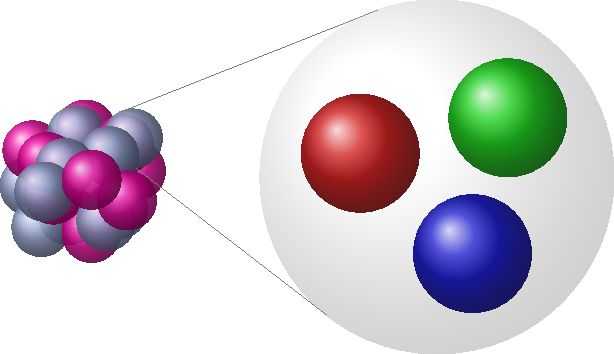
\includegraphics[width=0.65\textwidth]{figures/picturebook/particles}
    % Caption
    \caption[A visualization of quarks as fundamental particles within the proton.]{
        Quarks, visualized as red, blue, and green spheres, are fundamental particles contained within the proton.
        %
        This is only a visualization -- quarks are pointlike, as far as we know, and among the smallest known pieces of our universe.
    }
    % Figure Label
    \label{fig:picturebook_particles}
\end{sourcefigure}


% -----------------------------------
% Jets Section:
% -----------------------------------
\begin{sourcefigure}[t!]
    % Figure graphics
    \centering
    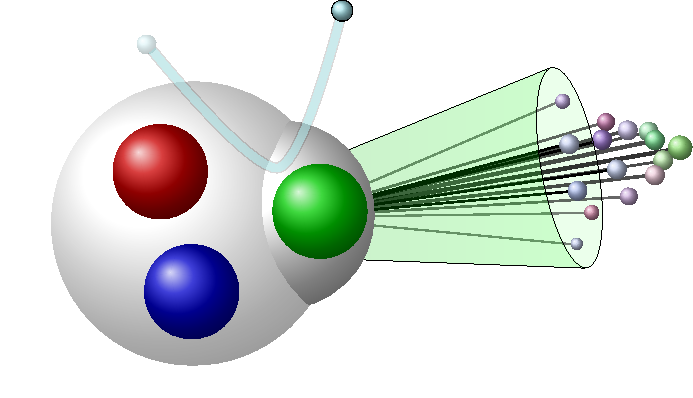
\includegraphics[width=0.6\textwidth]{figures/picturebook/dis-1}
    \hfill
    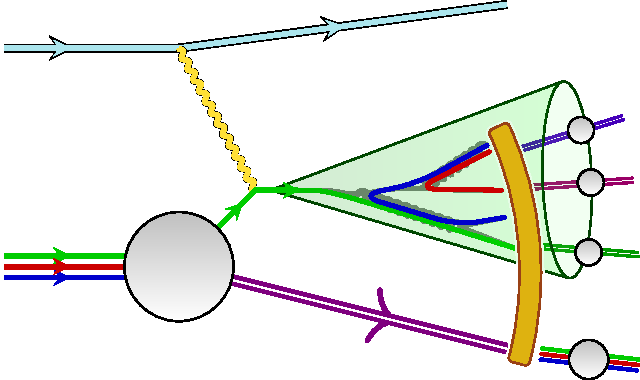
\includegraphics[width=0.6\textwidth]{figures/picturebook/dis-2}

    % Caption
    \caption[A visualization of jets formed by ejecting a quark from a nucleon during high energy scattering.]{
        Jets, collimated sprays of hadronic particles visualized as green cones, are formed when quarks (or gluons) are pushed out of their confines during a high-energy particle collision and undergo a cascading series of ``decays'' called the partonic cascade.
        % https://indico.cern.ch/event/492098/contributions/1169736/attachments/1356309/2050123/QCD2.pdf#page=21
    }

    % Figure Label
    \label{fig:picturebook_jets}
\end{sourcefigure}


% -----------------------------------
% Substructure Section:
% -----------------------------------
\begin{sourcefigure}[t!]
    % Figure graphics
    \centering
    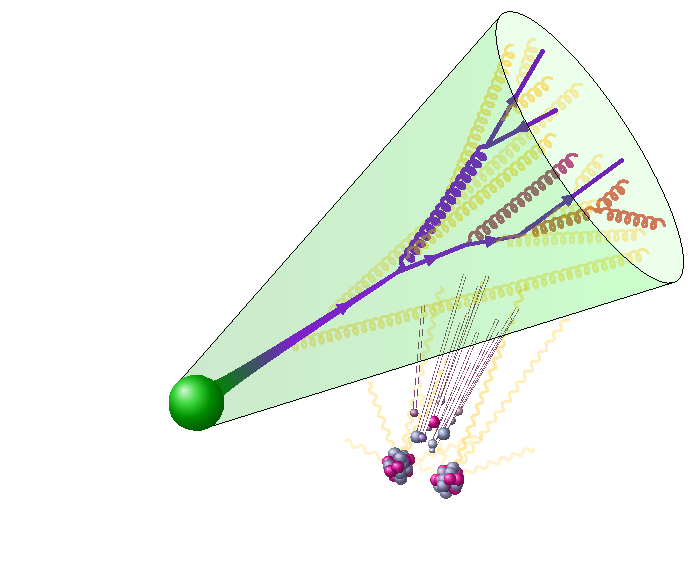
\includegraphics[width=0.8\textwidth]{figures/picturebook/jet-contamination}

    % Caption
    \caption[A visualization of the low-energy contamination within jets, whose removal is the goal of jet grooming.]{
        The goal of \emph{jet grooming} is to recover the information of high-energy jet substructure representing the physics of high energy quarks and gluons (visualized as dark, opaque lines, with darker colors/more opacity indicating higher energy) despite obfuscation from soft distortions (hadronization, detector effects) and additive contamination (pileup, underlying event).
    }

    % Figure Label
    \label{fig:picturebook_substructure}
\end{sourcefigure}


% -----------------------------------
% Event Shapes Section:
% -----------------------------------
\begin{sourcefigure}[t!]
    % Figure graphics
    \centering
    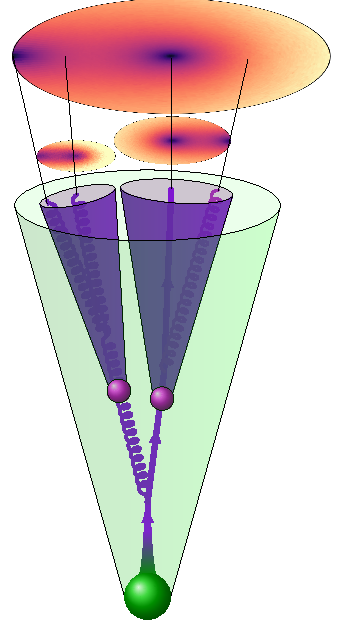
\includegraphics[width=0.38\textwidth, angle=-50]{figures/picturebook/fractal-substructure}

    % Caption
    \caption[A visualization of energy-weighted correlations capturing correlations between different high-energy structures within jets at different scales. \sam{incomplete, want bunch crossings rather than nuclei}]{
        Energy-weighted correlators capture correlations between high-energy structures within jets, such as particles (purple/black lines) or subjets (purple cones).
        %
        The explicit example of the resolved 3-point energy correlators of \Chap{ewocs}, compute using real collider data, are shown as colored disks above the jet to visualize energy-weighted correlations at different angular scales.
        %
        The higher energy regions of the cartoon jet depicted here are represented by higher values of the associated resolved energy correlator, and darker colors in the associated colored disks.
        %
        \sam{incomplete, want bunch crossings rather than nuclei}
    }
    % Figure Label
    \label{fig:picturebook_eventshapes}
\end{sourcefigure}




The story of \gls{qcd} is tightly intertwined with the story of \textit{renormalization} -- the way physical phenomena change as a function of scale.
%
It gives us a powerful framework for understanding how large structures emerge from smaller pieces, and we will barely scratch its incredibly vast implications in this thesis -- not for lack of trying!

Let's get our bearings.
%
As in \Fig{picturebook_universe}, we will zoom in on the universe from the largest scales to the smallest.
%
The largest, super-galactic structures we know of in the universe -- galactic filaments larger than 1 billion light years in length, \(10^{25}\) times larger than the \(\mathcal{O}(1 \text{ meter})\) macroscopic objects of our daily lives -- are composed of smaller pieces:
%
superclusters, then clusters, then groups of galaxies.
%
The ``small'' galaxies themselves tend to have a size of ``only'' \(10^{20}\) meters.
%
Our solar system is around \(10^{12}\) meters in size and our gorgeous planet earth only around \(10^7\) meters.
%
The vast separation of these scales -- the super-galactic, the galatic, the terrestrial -- is an amazing and curious feature:
%
the piecing together of small structures occurs at distances far larger than any individual piece could hope to traverse or understand.



The small structures themselves, however, are also immensely complicated.
%
The surface of the earth alone is home to an unimaginable number of ecological systems.
%
Each human home has an intricate and beautiful story.

And we ourselves are not the end.
%
Cells (for humans, \(10^{-4}\)-\(10^{-5}\) m), within them atoms (for hydrogen, around \(10^{-10}\) m) -- and protons, neutrons (\(10^{-18}\) m), electrons (pointlike, as far as we know) -- are the building blocks of our experience.

This thesis is a (\textit{very}) short sentence in the grand tale of the smallest scales we have been able to study with the scientific method%
\footnote{
    Don't tell the string theorists and quantum gravitists -- they have been able to probe even deeper with the power of pure thought!
}.
%
Like the largest scales of the known universe, the quarks and gluons within protons and neutrons, described by \gls{qcd}, are the smallest pieces we can experimentally probe.
%
They are the limits to our fundamental understanding of the universe.

The theory of \gls{qcd} describes over \(99.9\%\) of the visible mass of the universe, and therefore the majority of what we might see if we were able to zoom deeply into the structures of the macroscopic objects of our daily experience.%
\footnote{
    The mass of the hydrogen atom, for example, is more than \(99.9\%\) accounted for by the mass of the proton within, and the electronic (electroweak) contribution to mass its less than \(0.1\%\).
}.
%
As a human, computer, or whatever you are, it likely describes the vast majority of your internal make-up.
%
We deserve to know what we are made of.
%
So let us now take for granted that we want to understand it.


The story of humanity's \textit{discovery} of \gls{qcd} occurs on the stage of particle collisions:
%
by slamming big objects together hard enough, we can break them apart and see the smaller pieces that lie inside.
%
To begin, we must understand the cast and the milieu:
%
particles themselves, and the way they collide.


\Glspl{particle}, such as the quarks within the proton visualized in \Fig{picturebook_particles}, are covered in \Chap{particles}.
%
In \Sec{sm-scattering-review}, we discuss what they are, the framework of quantum field theory used to describe them, and the principles of scattering that we will use to understand the quarks and gluons that compose our universe at the smallest scales.

We will discuss the universal features of quarks and gluons (partons) as they emerge from scattering experiments in \Sec{universal-features}.



In \Chap{jets}, we will discuss a beautiful complication to the story:
%
the high-energy quarks and gluons which emerge when we break apart a proton themselves contain more quarks and gluons%
\footnote{
    Hence the name ``Particles Inside Particles'' for this thesis.
}.
%
The resulting fractal-like structures emerging from scattered quarks and gluons, visualized in \Fig{picturebook_jets}, are called \glspl{jet}.
%
In \Sec{parton-shower}, we discuss and roughly derive the partonic cascade model of energy flow within the quark, and of jet formation.
%
Unfortunately, experiments are messy, and to understand the behavior of partons we need to see through a contaminating haze of low-energy pollution, discussed in \Sec{low-energy-pollution}.



In \Chap{grooming}, we introduce one of the simplest ways to overcome low-energy pollution:
%
the \textit{grooming} of jets.
%
Jet grooming isolates the high-energy structures within jets (visualized as the dark opaque lines of \Fig{picturebook_substructure}) by removing the low-energy contamination (the lighter, more transparent lines of \Fig{picturebook_substructure}).
%
In \Sec{traditional-grooming}, we discuss traditional strategies for \gls{jet-grooming}.
%
In \Sec{piranha}, we introduce a new strategy for \textit{continuous} jet grooming, called \PIRANHA{} grooming, originally discussed in \Reff{Alipour-Fard:2023prj} by myself, Eric Metodiev, Patrick Komiske, and Jesse Thaler.
%
In \Secs{discontinuity}{grooming-pheno}, we present formal and phenomenological discussions, respectively, of the benefits of continuity exemplified by \PIRANHA{} grooming.




In \Chap{ewocs}, we present a distinct method for peering through pollution in particle collisions:
%
the use of \textit{energy-weighted correlations}.
%
The features of energy-weighted correlations are a bit more abstract than those of jet grooming, but we attempt to visualize them in \Fig{picturebook_eventshapes}, where darker regions are associated with higher energies (and thus larger energy-weighted correlations).
%
In \Sec{eec}, we introduce the simplest type of energy-weighted correlation, known as the Energy-Energy Correlator (EEC), which probe angular correlations between pairs of particles in particle collisions.
%
In \Sec{new-angles}, we discuss multi-particle generalizations of the EEC, and the parameterization given in \Reff{Alipour-fard:2024szj} by myself, Ankita Budhraja, Jesse Thaler, and Wouter Waalejwin.
%
In \Sec{ewocs}, we go beyond the limitations of angular correlations, introducing the generic concept of \glslink{ewoc}{Energy-Weighted Observable Correlations} from our work in \Reff{Alipour-fard:2025dvp} by myself and Wouter Waalejwin.


70 years ago, humanity discovered new particles that nobody expected.
%
We had only the brilliant minds of humanity's experimental and theoretical physicists to battle against the looming darkness of incomprehension.
%
The triumph of these physicists in the theory of \gls{qcd} has led to a rich new story of quarks, gluons, and the inner structure of jets.
%
Thanks to their effort, and that of their successors, we now have methods to piece together the properties of the smallest known constituents of 99.9\% of the visible mass of our universe from high-energy particle collisions, even through the ubiquitous haze of contaminating pollution that obfuscate scattering events.
%
I hope to lucidly convey a small piece of this story.
 % TOGGLE
% ==============================================
% Has no appendices (appendices auto-add new line to toc..?),
% so we add a new toc line manually here
\addnewlinetotoc{}
\clearpage{}

% ==============================================
\chapter[Particles]{Particles}
\markboth{\small \textsc{Chapter \thechapter}: \bf Particles}{}

\label{chap:particles}

% \epigraph{Never trust an parton: they make up everything...}{}

\epigraph{The proton isn’t actually bound, if you take my meaning: a little scratch — and it is blown to pieces.}{Yuri L. Dokshitzer, ``Perturbative QCD Theory'' \cite{Dokshitzer:1998nz}}

By a loose definition of ``particle physicist'', we might say that the first particle physicists were the first curious animals on earth to be amazed by the fact that by slamming two rocks together, they could see the ingredients the rocks contained within.
%
I conjecture that this may have been around 300 million years ago, during the Triassic period, when the first dinosaurs and proto-mammals were roaming the earth.


We have come a long way since then.


Almost everything that humanity knows about our subatomic universe, we know through similar exploits:
%
our experiments and theory of scattering.
%
The study of scattering is the study of the question ``what do things do when we slam them together?''
%
Strikingly, we have discovered that the scattering of subatomic objects in quantum mechanics has incredible similarities to the scattering of rocks that our millions-of-years-older ancestors saw.
%
There is conservation of momentum;
%
slowly moving objects often simply bounce off one another without significantly changing;
%
and if we scatter two objects at high enough energies, we can see what was inside.
%
Scattering will show us that \emph{even \textit{fundamental} particles have a rich internal structure} that we will explore in order to understand the behavior of our microscopic universe.


The main triumph of this chapter is the introduction of \vocab{partons}:
%
the main actors of modern particle physics whose main role is to compose all other matter, and can be thought of as the fundamental moving pieces in a particle collision experiment.
%
As we introduce the basics of the \glsfirst{sm} and \glsfirst{qcd}, we will discuss what we know about particles and partons, and how we know it.
%
We focus on quarks and gluons, the fundamental particles described by \gls{qcd} (our theory of the strong force) which are the central focus of this thesis.
%
Throughout this thesis, we will also run into the photon, the \(W\)-boson, and even \textit{composite} particles (such as the proton and neutron) that themselves are composed of quarks, gluons, photons, and more.
%
We will make some quantitative predictions which accentuate the profound strangeness of quantum field theory and foretell the emergence of high-energy jets -- proxies for partonic degrees of freedom that we discuss in the next chapter, and which themselves contain many, many particles.

In the analogy of particle collisions as the slamming together of rocky geodes with beautiful internal structure, the partons are like the molecules which make up the rock/crystal itself.
%
When the two rocks collide, it is really the tiny molecules that make them up which are interacting.
%
In scattering the rocks, it is the interactions of these tiny, indiscernible pieces are what produce macroscopic effects:
%
the breaking of the rocks, the clouds of rock dust, and the unveiling of the breathtaking geodes within.


% ==============================================
\section{The physical picture}
% ==============================================

% -----------------------------------
% Picturebook figure
% -----------------------------------
\reusefigure[ht]{picturebook_particles}

Rather than scattering rocks, we will be concerned with the scattering of subatomic particles.
%
But what is a particle?
%
To answer this, let us point out that an electron moving to your left is a different state than an electron moving to your right;
%
furthermore, if you say that it is moving to the left, someone facing you will say that it is moving to the right!
%
But you should both agree, regardless of the direction of its motion or spin, that it is the same \textit{type} of particle:
%
an electron.
%
So a particle should be a \textit{set} or \textit{collection} of states which different (inertial) observers agree correspond to the same particle.

\begin{definitionbox}{Particle}{particle}
    A \vocab{particle} is a \textit{set} of quantum states characterized by mass, spin, and charge -- their \textit{quantum numbers} -- such that:
    \begin{itemize}
        \item
            it is \vocab{invariant} under Poincar\'e transformations:
            %
            the overall set of states remains unchanged under translations in space/time, rotations, and boosts;


        \item
            It is \vocab{irreducible}:
            %
            it contains no proper invariant subsets.
    \end{itemize}
    In technical language, we often say that a particle is \textit{an irreducible representation} (irrep).
\end{definitionbox}


\remark{}{
    Really, this definition holds in flat spacetimes when using only massive particles.
    %
    The story does not end there, however, and beyond there is a forest of subtleties which lie far beyond the scope of this thesis.
    %
    One important subtlety is that in \textit{gauge theories} such as \gls{qcd} and the \gls{sm}, even the description of fundamental particles as irreducible representations of the Poincar\'e group has flaws;
    %
    in technical language, gauge invariant states of a gauge theory are associated with additional gauge fields and asymptotic charge that are not encompassed by the definition of particles as irreps of the Poincar\'e group.
    %
    See e.g. the influential early work of \Reff{Kulish:1970ut}, which states that ``the representation of the Poincar\'e group ... acting in the physical Hilbert space ... does not contain discrete irreducible terms with nonvanishing mass. In other words, one can say that the relativistic concept of a charged particle does not exist.''
    %
    The idea that the notion of ``particle'' must be modified in theories with massless particles manifests in several frameworks.
    %
    The framework closest to the ideas presented in this work (see especially \Sec{splitting-functions}) states that we must stop thinking about quantum amplitudes and begin thinking about \emph{inclusive probabilities} \cite{Yennie:1961ad}.
    %
    This perspective can also be connected to the framework of \emph{infraparticles} \cite{Schroer:1963gw,Schroer:2008gd} (also the Faddeev-Kulish framework \cite{Dirac:1955uv,Kulish:1970ut}).
}

Particles interact according to forces such as electromagnetism, the strong force, and the weak force.
%
In quantum field theory, particles are interpreted as excitations of underlying \textit{fields} -- mathematical objects which, like the more familiar electric field, occupy all of space -- with each type of particle corresponding to a different quantum field.
%
The interactions of these \textit{fields}, for our purposes encoded by a \textit{Lagrangian}, can be used to predict the interactions and dynamics of the associated particles.

Through the unified framework of \textit{scattering}, experimental and theoretical studies of particles together allow us to deduce the Lagrangian that describes the universe.
%
By scattering particles together and measuring what comes out, and comparing to theoretical calculations and predictions, we are able to determine how well a given quantum field theory predicts the behavior of the actual universe.

Experimental and theoretical studies of scattering are usually phrased in terms of \glspl{xsec}, differential cross sections, or probability distributions associated with scattering outcomes.
%
The \vocab{cross section} associated with a certain scattering outcome, denoted by \(\sigma\), characterizes how strong the interactions producing the outcome are.
%
The larger the cross section, the stronger the interactions.
%
\vocab{Differential cross sections} and \vocab{probability distributions} are more detailed functions which characterizes how much of the cross section is associated with particular regions of phase space for the scattering outcome.


The goal of this chapter is to hone our intuition and prepare us for the remainder of the thesis.
%
In \Sec{sm-scattering-review}, we review the ingredients of the \gls{sm}, focusing on the scattering of the particles of \gls{qcd}.
%
\Sec{universal-features} explores the features of quarks and gluons in high-energy scattering experiments, beginning with rough derivations of their universal behavior and concluding with a general diagrammatic presentation of fixed-order computations.



% ==============================================
\section{Uncovering the Quantum Universe}
% ==============================================
\label{sec:sm-scattering-review}

Quantum field theory (\gls{qft}) is our simplest framework for relativistic quantum mechanics, and provides elegant solutions to a huge number of conceptual difficulties.%
\footnote{
See, for example, the early chapters of Daniel Harlow's  \textit{Notes on Quantum Field Theory} \cite{Harlow:2024zz}, as well as \href{https://arnold-neumaier.at/physfaq/topics/multi.html}{a blog post of Arnold Neumeier on multiparticle relativistic quantum mechanics, \texttt{available at this https url}}.
}
%
\Gls{qft} was developed first as a tool to describe the fundamental constituents of our universe -- a story that has culminated in the development of \gls{qcd} and the \gls{sm}.%
\footnote{
    And, depending on your company, string theory.
}
%
Today, however, \gls{qft} is a powerful framework for quantum mechanics even in a wide variety of observed phenomena, including non-relativistic phenomena ranging from nuclear transitions to superfluidity and superconductivity.

Our focus in this thesis, however, remains on the smallest building blocks of the \gls{sm} and \gls{qcd}, which we introduce in \Sec{sm-qcd}, and therefore on the framework of \gls{scattering} we use to understand them, which we introduce in \Sec{scattering}.
%
In \Sec{observables}, we introduce \glspl{observable} as theoretical probes of the physics of scattering.
%
In \Sec{irc-safety}, we introduce \glslink{irc-safety}{infra-red and collinear (IRC) safety} as a property of the (perturbatively) well-behaved \glspl{observable} we use in this thesis..
%
\Sec{phd}, which may be skipped on a first reading, discusses why we can trust perturbative calculations involving quarks and gluons, given that the \gls{qcd} matter of our universe is bound up into hadrons.
%
The discussion of this section will leave us ready for whatever may come in the concrete calculations that follow in the remainder of this thesis.


% -----------------------------------
\subsection{Models of the Quantum Universe}
% -----------------------------------
\label{sec:sm-qcd}

\epigraph{What could be more natural than to unite these spin-one bosons into a multiplet of gauge fields?}{Steven Weinberg, \textit{A Model of Leptons} \cite{Weinberg:1967tq}, 1967}

The \gls{sm} is our best theory by far for describing our observations of particle scattering, and contains the theory of \gls{qcd} which describes the interactions of the quarks, gluons, and jets which are the subject of this thesis;
%
it contains all known particles, and the main complaint of particle physicists today is that there are too few disagreements between experimental and theoretical results to point towards new and better theories.

This thesis explores the physics of \gls{qcd}, which describes \(99.9\%\) of the observable matter predicted by the \gls{sm}, and in particular describes the quarks, gluons, and hadronic jets produced in high-energy particle collisions.
%
Therefore, before a more detailed exposition of the \gls{sm}, let us note immediately that
\begin{answer}
    The physics we explore in this thesis is encoded in the massless \gls{qcd} Lagrangian
    \begin{align}
        \label{eq:qcd-lagrangian}
        \mathcal{L}_\text{QCD}
        &=
        - \frac{1}{4} G\indices{^a_{\mu\nu}} G^{a\,\mu\nu}
        +
        i \overline{q}_i \slashed{D} q_i
        \,,
    \end{align}
    %
    where the \(q_i\) are Dirac fermions encoding the quark and anti-quark fields, \(i\) denotes the quark \textit{flavor} (for the purposes of this thesis \(i \in \{\)up, down, charm, strange, bottom\(\}\)), and the \(G\indices{^a_{\mu\nu}}\) are the gluon field strength tensors describing an SU(\(N_c\)) gauge theory with the \textit{number of colors} \(N_c = 3\).
\end{answer}

Readers who are interested in pursuing the theory of \gls{qcd} directly may wish to proceed directly to the \gls{qcd} Feynman rules in \Eqs{gluon_main_frules}{quark_main_frules}, the discussion of particle collisions and collider observables in \Secs{scattering}{observables}, the discussion of partonic scattering in \Sec{universal-features}, or even our discussion of jets in \Chap{jets}.
%
Nonetheless, we will take this opportunity to discuss the more general framework of gauge theory and the \gls{sm}.


The \gls{sm} is ultimately an elegant and extremely non-trivial extension of the theory of electromagnetism.
%
There is an infinity of concepts within the \gls{sm} that we will not cover -- we will not perform explicit loop-level calculations of quantum effects, and we will ignore higher dimension operators, the hierarchy problem (see especially \Reff{Koren:2020pio}), discrete  symmetries (see \Reff{Koren:2022bam}, also with a beautiful explanation of proton stability in the \gls{sm}), and an enormous amount of beautiful phenomenology and formal theory, for a start.
%
The \gls{sm} has a rich formal structure that we will ignore as well, from the classical and quantum geometric structures of Yang-Mills theory to the modern developments of non-invertible symmetries (see e.g. \Reffs{Cordova:2022fhg,Cordova:2022qtz}).
%
Instead, we focus specifically on the physics that will take us to an understanding of jets.
%
We will take a shortcut to the \gls{sm} through the theory of electromagnetism, before focusing exclusively on \gls{qcd}.

\remark{}{
    A more in-depth exposition of \gls{qft} would require a great deal of effort, and distract from the physics of quarks, gluons, and jets that we wish to explore in this thesis.
    %
    Nonetheless, I mention that some of my favorite introductory resources on \gls{qft} are Mark Srednicki's \underline{Quantum Field Theory} \cite{Srednicki:2007qs} and Daniel Harlow's \textit{Notes on Quantum Field Theory} \cite{Harlow:2024zz}.
    %
    The latter in particular gives a sense of the full, deep flavor of \gls{qft} from algebraic, calculational, and intuitive perspectives through a detailed discussion that is not usually emphasized in introductory discussions of \gls{qft}.
}


The theory of electromagnetism describes the physics of electric and magnetic fields is often described by an energy functional/Hamiltonian dependent on the electric and magnetic fields.
%
However, it is often far easier to use \textit{gauge fields} to describe the physics of the electric and magnetic fields.
%
The use of gauge fields make manifest the presence of the symmetries of special relativity -- the Lorentz symmetries combining rotations and boosts -- in the theory of electromagnetism.
%
The gauge fields of electromagnetism are the \textit{electric potential} \(\phi\) and the \textit{vector potential} \(\vec{A}\), which may be grouped into a Lorentz four-vector
\begin{align}
    A^\mu &\reppedby \le(\phi, \, \vec{A}\ri)
    \,,
\end{align}
which encodes the electric and magnetic fields in the \vocab{field strength tensor},
\begin{align}
    F_{\mu\nu} &= \partial_\mu A_\nu - \partial_\nu A_\mu
    \,.
\end{align}
%
The electric and magnetic fields take the form%
\footnote{
    Note the unfortunate use of the \((+,-,-,-)\) metric.
}
\begin{align}
    E^i &= F_{0i} = -\partial_t A^i - \partial^i \phi
    \\
    B^i
    &=
    \half \epsilon^{ijk} F_{jk}
    =
    \le(\nabla \cross A\ri)^i
    \,,
\end{align}
%
The principles of special relativity, and hence the use of gauge fields, will be especially important for us as we study high-energy particle collisions with outgoing particles moving near the speed of light.
%
Gauge fields also allow a more easy generalization of quantum electrodynamics (QED), with electric and magnetic fields, to \gls{qcd}, with the creatively named chromo-electric and chromo-magnetic fields.
%
In particular, under the U(1) \vocab{gauge transformation}
\begin{align}
    \le(\partial_\mu - i e A_\mu\ri)^\prime
    :=
    e^{-i e \alpha(x)}
    \le(\partial_\mu - i e A_\mu\ri)
    e^{i e \alpha(x)}
    \,,
\end{align}
where \(\alpha(x)\) is arbitrary, the gauge field is transformed into
\begin{align}
    A^\prime_{\mu}
    =
    A_\mu
    -
    \partial_\mu \alpha
    \,.
\end{align}
%
This transformation is called a U(1) gauge transformation because the factor \(U := U(x) := e^{-i e \alpha(x)}\) is a \(1 \times 1\) \textit{unitary matrix}, with \(U^\dagger U = 1\), and U(1) is the group whose multiplication structure is isomorphic to the set of 1\(\times\)1 unitary matrices.
%
We sometimes say that \(U = e^{-i e \alpha(x)}\) corresponds to a representation of U(1) at every point \(x\), called the U(1) \textit{gauge group}, with charge \(e\).
%
The object \(D_\mu := \partial_\mu - i e A_\mu\) is called the \textit{covariant derivative} (in the representation of U(1) with charge \(e\)).


The interpretation of electromagnetism in terms of gauge fields has a beautiful geometric interpretation which, unfortunately, we will not discuss.
%
We will mention briefly, however, that the field strength tensor is a type of \textit{curvature} in the geometric interpretation, and in particular
\begin{align}
    \frac{i}{e} \, \comm{D_\mu}{D_\nu} =: F_{\mu\nu}
    \,.
\end{align}
%
The representation of \(F_{\mu\nu}\) makes it clear that it is invariant under the gauge transformations, and therefore there are changes in \(A_\mu\) that do not affect the physical electric and magnetic fields.
%
The gauge fields are \textit{un-physical} in the sense that they contain extra degrees of freedom that are not present in electromagnetism;
%
the invariance of \(F_{\mu\nu}\) under gauge transformations indicates the \textit{redundancy} of the description of electromagnetism in terms of gauge fields.

Including a massless electron \(e\) and the positron \(\overline{e}\) -- Weyl fermion fields whose properties are discussed in standard texts on quantum field theory (see, e.g. Mark Srednicki's \underline{Quantum Field Theory}, Part II \cite{Srednicki:2007qs}) -- yields the Lagrangian for massless \textit{quantum electrodynamics} (QED):
\begin{align}
    \mathcal{L}_\text{QED}
    =
    -\frac{1}{4}F_{\mu\nu} F^{\mu\nu}
    +
    i \overline{e} \, \overline{\sigma}^\mu D_\mu \, e
    =
    -\frac{1}{4}F_{\mu\nu} F^{\mu\nu}
    +
    i \bar{\Psi} \slashed{D} \Psi
    \,,
\end{align}
where \(\Psi = \le(e, \overline{e}\ri)\) is a Dirac spinor that groups together the left- and right-handed Weyl spinors \(e\) and \(\overline{e}\).
%
\(\overline{\sigma}^\mu \reppedby \le(I, \vec{\sigma}\ri)\) is a four-vector whose components are each 2\(\times\)2 matrices;
%
it is an \vocab{invariant symbol}%
\footnote{
    Invariant symbols are also known as a Clebsch-Gordan coefficients of the associated group.
    %
    See \href{https://web.physics.ucsb.edu/~mark/ms-qft-DRAFT.pdf\#page=415}{Mark Srednicki's \underline{Quantum Field Theory}, Chapters 34, 35, and 70.} \cite{Srednicki:2007qs}.
}
%
of the Lorentz group.
%
The Lagrangian of massless QED contains a free photon (gauge field), encoded by the piece \(\mathcal{L} \supset -F_{\mu\nu}F^{\mu\nu}/4\), a free fermion, encoded by \(\mathcal{L} \supset i\overline{e} \overline{\sigma}^\mu \partial_\mu e = i \bar{\Psi} \slashed{\partial} \Psi\), and an interaction \(\mathcal{L} \supset A^\mu J_\mu = i\overline{e} \overline{\sigma}^\mu A_\mu e = i \bar{\Psi} \slashed{A} \Psi\) between the photon and the electromagnetic current generated by the presence of the electron and positron.


The generalization of electromagnetism that appears in the \gls{sm} is known as \textit{Yang-Mills theory}.
%
In Yang-Mills theory, the group U(1) which encodes the gauge transformation properties of \(A_\mu\) is upgraded to a more general group (in particular, a Lie group).
%
The most common example -- and the example relevant for \gls{qcd} and the \gls{sm} -- is the group SU(N), isomorphic to the set of \(N\times N\) unitary matrices with determinant 1.


\remark{}{
    The classical properties of Yang-Mills theory, even with matter (electrons in QED, quarks in \gls{qcd}, and even the Higgs boson in the \gls{sm}), can be explained elegantly in terms of geometric concepts (connections, principal bundles, horizontal subspaces, spinor bundles, etc.).
    %
    Such an explanation is far outside the scope of our discussion, but some relevant mathematical resources include \Reffs{spinorial_chessboard,Hamilton:2017gbn}.
}

In Yang-Mills theory with gauge group SU(N), we instead write \(U_{(R)} = e^{-i g T_{(R)}^a \alpha^a(x)}\) is upgraded to an element of (a representation of) SU(N), where the \(\{T^a_{(R)}\}\) are linearly-independent, traceless matrices:
%
the generators of SU(N) in the representation \(R\).
%
The index \(a\) takes values in \(a \in \{1,\,\cdots,\,N^2-1\}\), and in any representation the generators are guaranteed to satisfy the condition
\begin{align}
    \comm{T^a_{(R)}}{T^b_{(R)}}
    =
    i f^{abc} T^c_{(R)}
    \,,
\end{align}
for geometric reasons that we do not cover here.
%
The \(f^{abc}\) are numbers, and are called the \vocab{structure constants} of the group.
%
The generators are conventionally chosen to satisfy
\begin{align}
    \Tr\le(T_{(R)}^a T_{(R)}^b\ri) = T_R \delta^{ab}
    \,,
\end{align}
where the factor 1/2 is called the \textit{Dynkin index} (after mathematician Eugene Dynkin), which we will discuss more when we introduce the Feynman rules of \gls{qcd}.
%
These requirements on the generators can be used to show that the \(f^{abc}\) are completely antisymmetric with respect to exchange of any two indices.


The covariant derivative in the representation \(R\) also becomes a matrix, and takes the form
\begin{align}
    D_{(R)\,\mu}
    :=
    \partial_\mu
    -
    i g T^a_{(R)} A^a_\mu
    \equiv
    \partial_\mu
    -
    i g A_{(R)\,\mu}
    \,,
\end{align}
where the gauge transformation now takes the form
\begin{align}
    D^\prime_{(R)\,\mu}
    :=
    U_{(R)}
    D_{(R)\,\mu}
    U^\dagger_{(R)}
    \,,
\end{align}
and \(U_{(R)} := U_{(R)}(x)\) is dependent on the space-time position at which it is evaluated.
%
In terms of the gauge field \(A^a_\mu\), we have
\begin{align}
    T^a_{(R)} A^{\prime\,a}_\mu
    =
    A_\mu^b
    U_{(R)} T^b_{(R)} U^\dagger_{(R)}
    +
    \frac{i}{g} U_{(R)} \partial_\mu U^\dagger_{(R)}
    \,,
\end{align}
and, when the \(\alpha^a(x)\) are small enough to discard terms of \(\mathcal{O}(\alpha^2)\),
\begin{align}
    A^{\prime\,a}_\mu
    =
    A^{a}_\mu
    -
    \partial_\mu \alpha^a
    +
    g f^{abc} A^b_\mu \alpha^c
    \,.
\end{align}
% Check by explicit computation.
% also, plus sign in final term on pg 5 of Nate's 229B Lecture 12

The field strength tensor is
\begin{align}
    \label{eq:non-abelian-field-strength}
    F_{(R)\,\mu\nu}
    \equiv
    T^a_{(R)}
    F\indices{^a_{\mu\nu}}
    :=
    \frac{i}{g}
    \comm{D_{(R)\,\mu}}{D_{(R)\,\nu}}
    =
    T^a_{(R)}
    \le(
        \partial_\mu A^a_\nu - \partial_\nu A^a_\mu
        + g f^{abc} A^b_\mu A^c_\nu
    \ri)
    \,.
\end{align}
The additional non-linearity of \(F\indices{^a_{\mu\nu}}\) may appear complicated or even innocuous in \Eq{non-abelian-field-strength}, but it has incredibly deep implications for the existence of \gls{qcd} -- it is the reason \gls{qcd} overcomes the weaknesses of the quantum field theories that precede it, leads to the asymptotic freedom of quarks and gluons discussed below, and allows us to perform perturbative calculations at high energies (this is discussed further in \Sec{phd}).


Matter also matters.
%
Quarks in particular will play a large role in our discussion.
%
A \textit{matter field} \(\varphi\) -- e.g. a scalar or fermion field -- \vocab{transforms under the representation \(R\)} (of the gauge group) if
\begin{align}
    \varphi^\prime(x) = U_{(R)}(x) \, \varphi(x)
    \,.
\end{align}
%
A gauge theory with fermions \(\{\psi_{i}\}\) transforming in the representations \(R_i\) of the gauge group and scalars \(\{\phi_k\}\) transforming in the representations \(R_k\) can be described in terms of the \vocab{Yang-Mills-matter Lagrangian}%
\footnote{
    Non-Lagrangian methods for understanding \gls{qft}, such as bootstrap methods (e.g. the \textit{amplitudes program} of \gls{qft}) and the operator product expansion, are also available.
    %
    They can provide more rigorous descriptions of quantum dynamics than we pursue in this thesis, but are often more technically difficult as well.
}.
%
With massless Weyl fermions (guaranteed in the \gls{sm} due to the chiral representations of the fermionic \gls{sm} matter content), in \(d=3+1\) dimensions, and ignoring higher-dimension operators, it takes the form
\begin{subequations}
    \label{eq:yang-mills-matter-lagrangian}
\begin{align}
    \mathcal{L}
    &=
    \mathcal{L}_\text{YM}
    +
    \mathcal{L}_\text{fermion}
    +
    \mathcal{L}_\text{scalar}
    +
    \mathcal{L}_\text{Yukawa}
    \,,
    \\
    \mathcal{L}_\text{YM}
    &=
    -
    \frac{1}{2} \Tr F_{\mu\nu} F^{\mu\nu}
    -
    \frac{1}{8 \pi^2}
    \epsilon^{\mu\nu\rho\sigma}
    \Tr
        \Theta_\text{CP}
        F_{\mu\nu}
        F_{\rho\sigma}
    \,
    \\
    \mathcal{L}_\text{fermion}
    &=
    i \sum_i \psi_i^\dagger \overline{\sigma}^\mu D_{(R_i)\,\mu} \psi_i
    \\
    \mathcal{L}_\text{scalar}
    &=
    \sum_k \le(D_{(R_k)}^\mu \phi_k\ri)^\dagger D_{(R_k)\,\,\mu} \phi_k
    -
    \sum_{k,\ell} \! {}^\prime
    \,\,
    m_{k\ell}^2
    \,\,
    \phi_k \, \phi_\ell
    \,\,
    S_{R_k R_\ell}
    +
    \text{h.c}
    \\
    \notag
    &\qquad\qquad
    +
    \sum_{k,\ell,m,n} \!\!\!\! {}^\prime
    \,\,
    \lambda_{k\ell m n}
    \,\,
    \phi_k \, \phi_\ell \, \phi_m \, \phi_n
    \,\,
    S_{R_k R_\ell R_m R_n}
    +
    \text{h.c.}
    \\
    \mathcal{L}_\text{Yukawa}
    &=
    \sum_{ij}
    \sum_{k} \! {}^\prime
    \,\,
    y_{ijk}
    \,\,
    \psi_i \,\psi_j \,\, \phi_k
    \,\,
    S_{R_i R_j R_k}
    +
    \text{h.c.}
    \,,
\end{align}
\end{subequations}
where the \(\sum'\) indicates a sum on both the scalar fields \(\phi_k\) and the complex conjugates \(\phi_k^\dagger\), the \(S\) are invariant symbols of the gauge group which project onto singlet representations and guarantee the invariance of the Lagrangian under gauge transformations, the charge-parity symmetry violating (CP-violating) parameter \(\Theta_\text{CP}\) -- usually multiplied by an additional factor of \(g^2\) -- is a central element of the gauge Lie algebra (almost -- see below) in the adjoint representation, and ``h.c.'' means hermitian conjugate.


\remark{}{
    The CP-violating terms in a gauge theory are usually denoted by a set of real parameters \(\{\theta_i\}\), one for each simple factor \(G_i\) of the gauge group \(G = \prod_i G_i\).
    %
    Each \(\theta_i\) multiplies the topological density \(\Tr(F^{(i)}_{\mu\nu} \tilde{F}^{(i)\,\mu\nu})\), associated with the field strength \(F^{(i)}\) of \(G_i\), and breaks CP symmetry when nonzero.
    %
    In the Lagrangian of \Eq{yang-mills-matter-lagrangian}, these terms are collectively encoded by \(\Theta_\text{CP}\), a single object in the center of the \emph{universal enveloping algebra} of the Lie algebra of the gauge group.%
    \footnote{
        The Lie algebra alone does not work.
        %
        For example, in SU(\(N\)), the adjoint representation of the algebra only contains traceless elements, while the CP-violating angle \(\theta_\text{CP}\) should be proportional to the identity to yield standard definitions.
        %
        Using the universal enveloping algebra in the adjoint representation allows for terms that are proportional to the identity, and thus the standard CP-violating angles \(\theta_\text{CP}\).
    }
    %
    Furthermore, a single degree of freedom of \(\Theta_\text{CP}\) can be removed for every anomalous global symmetry of \(\mathcal{L}\), and CP-violating angles associated with Abelian (U(1) or \(\mathbb{R}\)) factors of the gauge group can be ignored in topologically trivial spaces (see \Reff{Tong:2017oea} for a pedagogical introduction with an emphasis on the \gls{sm}).
}

\remark{}{
    The Lagrangian of \Eq{yang-mills-matter-lagrangian} is sufficient for classical, tree-level computations.
    %
    A complete description of quantum effects requires additional factors and, depending on the tools used in calculations, additional fields or constraints.
    %
    For example, counterterms are needed to understand the renormalization of fields and to produce finite results in scattering computations, a consistent treatment of non-covariant gauges requires the introduction of ghosts (or even anti-ghosts, in Batalin-Vilkovsky quantization), and when ghosts are present, a consistent description of Gribov ambiguities requires additional constraints (such as a restriction to a \emph{Gribov region} as in the Gribov-Zwanziger action).
    %
    In a bittersweet turn of events, the form of \Eq{yang-mills-matter-lagrangian} -- and indeed, the much simpler massless \gls{qcd} Lagrangian given in \Eq{qcd-lagrangian} -- will be sufficient for the work in this thesis, though more rigorous quantum treatments underlie the validity of the results we present.
}

\remark{}{
    There are additional non-trivial constraints on the matter content of a \gls{qft}, called \emph{gauge anomaly cancellation conditions}, which require that the charges of the matter fields are delicately balanced.
    %
    We will consider \gls{qcd} without the top quark in this thesis, and, though this effective theory \textit{does} have an anomaly, it is nonetheless consistent.
    %
    For an understanding of the properties of effective field theories which appear to carry anomalies, see the incredibly lucid account of \Reff{Preskill:1990fr}.
}


The full \gls{sm} is a rich and beautiful theory with gauge group%
\footnote{
    At least locally/up to global quotients by elements of the center of \(G_\text{SM}\), \(Z_\text{SM} = \{\mathbb{Z}_2, \mathbb{Z}_3, \mathbb{Z}_6\}\).
}
%
\(G_\text{SM}=\)SU(3)\(\times\)SU(2)\(\times\)U(1).
%
Armed with the SM gauge group, we are prepared to conquer the universe.
%
The SU(3) describes the dynamics of \gls{qcd}, while the SU(2)\(\times\)U(1) describes electroweak physics and (electroweak-scale) spontaneous symmetry breaking and provides an explanation of why we do not see the weak interaction in our daily lives.
%
The lexicon of \gls{sm} fields includes the gauge fields for each factor (SU(3), SU(2), and U(1)) as well as three copies of the Weyl fermion fields \(Q,\overline{u},\overline{d},L,\overline{e}\) (or \textit{``cuddly'' fields}, and we also note that the bars are part of the \textit{names} for the fields and do not indicate complex conjugation) with the following representations of the gauge group:
%%
\begin{center}
 \begin{tabular}{ |p{3cm}||p{3cm}|p{3cm}|p{3cm}|  }
 \hline
 Matter Field & SU(3) & SU(2) & U(1)\\
 \hline\hline
 \(Q = \binom{u}{d}\) & \(\mathbf{3}\)       & \(\mathbf{2}\) & \(1/6\)  \\
 \(\Bar{u}\)          & \(\bar{\mathbf{3}}\) & \(\mathbf{1}\) & \(-2/3\) \\
 \(\Bar{d}\)          & \(\bar{\mathbf{3}}\) & \(\mathbf{1}\) & \(1/3\)  \\
 \(L = \binom{\nu}{e}\) & \(\mathbf{1}\)       & \(\mathbf{2}\) & \(-1/2\) \\
 \(\bar{e}\) & \(\mathbf{1}\)       & \(\mathbf{1}\) & \(1\)            \\
 \hline
\end{tabular}
\end{center}
where we have enumerated the SU(2) components of the doublets \(Q\) and \(L\).
%
Finally, and famously, the \gls{sm} also contains a single \textit{Higgs boson}, a scalar field with representation
\begin{center}
 \begin{tabular}{ |p{3cm}||p{3cm}|p{3cm}|p{3cm}|  }
 \hline
 \(H\)       & \(\mathbf{1}\)       & \(\mathbf{2}\) & \(-1/2\) \\
 \hline
\end{tabular}
\end{center}
However, the development of the electroweak sector of the standard model is not the focus of this thesis, and we simply mention that the Lagrangian of the (renormalizable) \gls{sm} takes the general Yang-Mills-matter form given in \Eq{yang-mills-matter-lagrangian}.
%
The \gls{sm} Lagrangian is completely determined, up to the numerical values of its coupling constants, by the content of the tables above.
%
The Yukawa interactions involve the interactions of the Higgs boson with the fermionic matter fields which give mass to the particles of the \gls{sm}.


Instead, we will focus on the \textit{strong sector} of the \gls{sm}, the theory of \glslink{qcd}{Quantum Chromodynamics (QCD)}, after electroweak symmetry breaking.
%
We have already discussed the historical development of \gls{qcd} in \Chap{picturebook};
%
for now, we will re-motivate it by noting that it predicts and explains the observed spectrum of jets in high-energy particle collisions which probe the smallest, finest structures in the universe presently available to humanity\footnote{Again, don't tell the string theorists!}.
%
This means that \gls{qcd} explains the physics of the sub-sub-atomic universe.
%
It matches data, cross sections, structure functions.
%
As we have discussed in the introduction, the parton model for pointlike constituents of hadrons, introduced without a field theoretic interpretation by Feynman, eventually led to QCD as the complete theory of quarks and gluons.
%
Now we have the luxury of using perturbative QCD to understand their dynamics.
%
Nonetheless, with many rich open questions, the field of \gls{qcd} theory is still under development.

In this thesis, we are interested in the physics of the high-energy limit of QCD where quarks may be treated as massless, in the absence of electroweak effects and quark masses.
%
We will also ignore the possible presence of the CP-violating angle \(\theta_\text{QCD}\).
%
Therefore, the physics we explore in this thesis is encoded in the massless \gls{qcd} Lagrangian, presented in \Eq{qcd-lagrangian} and repeated below for convenience:
\begin{align}
    \mathcal{L}_\text{QCD}
    &=
    - \frac{1}{4} G\indices{^a_{\mu\nu}} G^{a\,\mu\nu}
    +
    i \overline{q}_i \slashed{D} q_i
    \,,
\end{align}
where the \(q_i\) are Dirac fermions encoding the quark and anti-quark fields, \(i\) denotes the quark \textit{flavor} (for the purposes of this thesis \(i \in \{\)up, down, charm, strange, bottom\(\}\)), and the \(G\indices{^a_{\mu\nu}}\) are the gluon field strength tensors describing an SU(\(N_c\)) gauge theory with the \textit{number of colors} \(N_c = 3\).

\remark{}{
    As before, a renormalized treatment requires the introduction of counterterms which we gloss over in our introductory treatment, but which may be found in any modern introductory textbook on quantum field theory.
    %
    We will largely ignore the top quark as well as electroweak effects in the formal discussions of this thesis, though we will include them in our phenomenological studies (e.g. we study the \(W\)-boson in \Chaps{grooming}{ewocs}).
}

The standard way to extract physical predictions about quantum-field-theoretic dynamics from a Lagrangian is the diagrammatic approach pioneered by Feynman, based on the path integral introduced by Dirac.
%
Looking at the Lagrangian, one follows a systematic procedure to extract a set of diagrammatic building blocks which give a concrete prescription for evaluating \textit{scattering amplitudes} -- tools used to predict the results of quantum scattering experiments.
%
Be careful:
%
the diagrams are not what is \textit{actually} happening to the quantum states involved in scattering.
%
Feynman diagrams are mathematical tools that we use to extract information about scattering within a particular theory, such as \gls{qcd}, allowing us to compare theoretical predictions to results from scattering experiments.


We introduce the concrete definitions of the scattering amplitudes \(\mathcal{M}\), and their use in describing particle collisions, in \Sec{scattering}.
%
First, however, let us introduce the tree-level \vocab{Feynman rules} for \gls{qcd}.

\remark{}{
    A standard way of determining the Feynman rules of a \gls{qft} is by calculating the generating functional -- the partition function in the presence of additional sources for fields.
    %
    Mark Srednicki's \underline{Quantum Field Theory} \cite{Srednicki:2007qs} is a wonderful pedagogical resource for the derivation of Feynman rules.
}


%%%%%%%%%%%%%%%%%%%%%%%  FEYNMAN RULES  %%%%%%%%%%%%%%%%%%%%%%%
\begin{answer}
\begin{center}
{\normalfont\Large\bfseries\sffamily The Rules for the Gluon Sector of QCD are:}
\end{center}

\begin{subequations}
\label{eq:gluon_main_frules}
\begin{align}
\raisebox{0pt}{
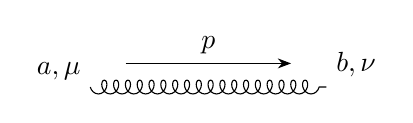
\begin{tikzpicture}
    \begin{feynman}
        % vertices
        \vertex (i) at (-1.5,0.0);
        \vertex (f) at (1.5,0.0);
        % edge labels
        \vertex [above left=-0.8pt and 0.0ptof i] (ti) {$a, \mu$};
        \vertex [above right=0.0pt and 0.0pt of f] (tf) {$b,\nu$};
        % diagram
        \diagram* {
            (i)
            -- [gluon, momentum=\(p\)]
            (f)
            ,
        };
    \end{feynman}
\end{tikzpicture}
}
\quad
:=
\quad
&
i\, \delta^{ab} \frac{-g_{\mu\nu} + (1-\xi) p_\mu p_\nu / p^2}{p^2 + i 0^+}
\\
\notag
\quad
\xrightarrow[\text{Feynman gauge}]{}
\quad
&
\delta^{ab} \frac{-i g_{\mu\nu}}{p^2 + i 0^+}
\end{align}


(in a covariant \(R_\xi\) gauge)

\begin{align}
\raisebox{-40pt}{
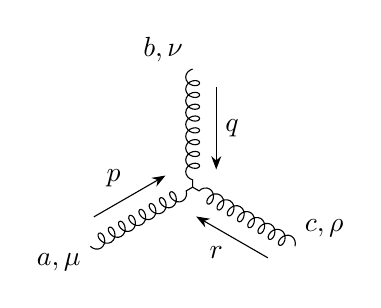
\begin{tikzpicture}
    \begin{feynman}
        % vertices
        \vertex (u) at (0,1.5);
        \vertex (l) at (-1.30,-0.75);
        \vertex (r) at (1.30,-0.75);
        \vertex (cen) at (0,0);
        % edge labels
        \vertex [below left=-0.8pt and 0.0ptof l] (tl) {$a, \mu$};
        \vertex [above left=-0.8pt and 0.0ptof u] (tu) {$b, \nu$};
        \vertex [above right=0.0pt and 0.0pt of r] (tr) {$c,\rho$};
        % diagram
        \diagram* {
            (l)
            -- [gluon, momentum=\(p\)]
            (cen)
            ,
            (u)
            -- [gluon, momentum=\(q\)]
            (cen)
            ,
            (r)
            -- [gluon, momentum=\(r\)]
            (cen)
        };
    \end{feynman}
\end{tikzpicture}
}
\quad
:=
\quad
-g f^{abc} \le[
    \begin{array}{rrr}
    (q-r)_\mu
    &
    g_{\nu\rho}
    &
    \\
    +&&
    \\
    (r-p)_\nu
    &
    g_{\rho\mu}
    &
    \\
    +&&
    \\
    (p-q)_\rho
    &
    g_{\mu\nu}
    &
    \end{array}
\ri]
\,.
\end{align}

\begin{align}
\raisebox{-40pt}{
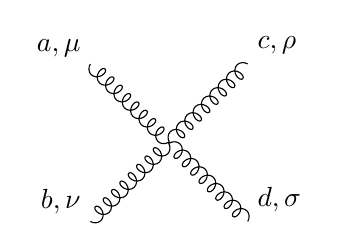
\begin{tikzpicture}
    \begin{feynman}
        % vertices
        \vertex (ul) at (-1.0,1.0);
        \vertex (ll) at (-1.0,-1.0);
        \vertex (ur) at (1.0,1.0);
        \vertex (lr) at (1.0,-1.0);
        \vertex (cen) at (0,0);
        % edge labels
        \vertex [above left=-0.8pt and 0.0ptof ul] (tu) {$a, \mu$};
        \vertex [above left=-0.8pt and 0.0ptof ll] (tl) {$b, \nu$};
        \vertex [above right=0.0pt and 0.0pt of ur] (tr) {$c,\rho$};
        \vertex [above right=0.0pt and 0.0pt of lr] (tr) {$d,\sigma$};
        % diagram
        \diagram*{
            (ul)
            -- [gluon]
            (cen)
            ,
            (ur)
            -- [gluon]
            (cen)
            ,
            (ll)
            -- [gluon]
            (cen)
            ,
            (lr)
            -- [gluon]
            (cen)
        };
    \end{feynman}
\end{tikzpicture}
}
\quad
:=
\quad
&
\le[
\begin{array}{rrr}
    -i g^2 & f^{\bar{e}ac} f^{\bar{e}bd} &\le(g_{\mu\nu} g_{\rho\sigma} - g_{\mu\sigma} g_{\nu\rho}\ri)
    \\
    -i g^2 & f^{\bar{e}ad} f^{\bar{e}bc} &\le(g_{\mu\nu} g_{\rho\sigma} - g_{\mu\rho} g_{\nu\sigma}\ri)
    \\
    -i g^2 & f^{\bar{e}ab} f^{\bar{e}cd} &\le(g_{\mu\rho} g_{\nu\sigma} - g_{\mu\sigma} g_{\nu\rho}\ri)
\end{array}
\ri]
\,.
\end{align}


External gluons, much like the photons describing the electromagnetic field, are \textit{polarized}.
%
Rather than coming with a propagator factor, as above, external gluons are accompanied by polarization vectors:
\begin{align}
\raisebox{-6pt}{
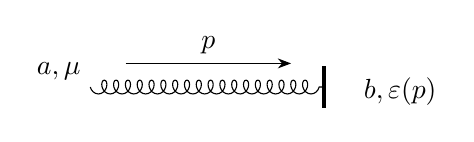
\begin{tikzpicture}
    \begin{feynman}
        % vertices
        \vertex (i) at (-1.5,0.0);
        \vertex (f) at (1.5,0.0);
        % edge labels
        \vertex [above left=-0.8pt and 0.0ptof i] (ti) {$a, \mu$};
        \vertex [above right=-10.0pt and 10.0pt of f] (tf) {$b, \varepsilon(p)$};
        % diagram
        \diagram* {
            (i)
            -- [gluon, momentum=\(p\),-{Bar[line width=1.5pt, width=15pt]}]
            (f)
            ,
        };
    \end{feynman}
\end{tikzpicture}
}
\quad
:=
\quad
\delta^{ab}
\,
\varepsilon^{*\, \mu}(p)
\end{align}
for outgoing, final-state gluons.
%
For initial state gluons with incoming momentum \(p\), the factor of \(\varepsilon^{*\,\mu}(p)\) is replaced by a factor of \(\varepsilon^\mu(p)\).

\end{subequations}
\end{answer}

\begin{answer}
\begin{center}
{\normalfont\Large\bfseries\sffamily The Rules for the Quark Sector of Massless QCD are:}
\end{center}

\begin{subequations}
\label{eq:quark_main_frules}
\begin{align}
\raisebox{0pt}{
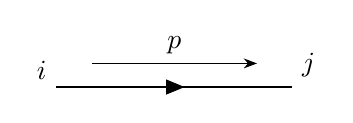
\begin{tikzpicture}
    \begin{feynman}
        % vertices
        \vertex (i) at (-1.5,0.0);
        \vertex (f) at (1.5,0.0);
        % edge labels
        \vertex [above left=-0.8pt and 0.0ptof i] (ti) {$i$};
        \vertex [above right=0.0pt and 0.0pt of f] (tf) {$j$};
        % diagram
        \diagram* {
            (i)
            -- [fermion, momentum=\(p\)]
            (f)
            ,
        };
    \end{feynman}
\end{tikzpicture}
}
\quad
:=
\quad
&
i\, \delta\indices{^j_i} \frac{\slashed{p}}{p^2 + i 0^+}
\end{align}

\begin{align}
\raisebox{-40pt}{
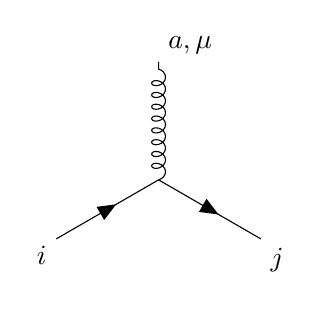
\begin{tikzpicture}
    \begin{feynman}
        % vertices
        \vertex (u) at (0,1.5);
        \vertex (l) at (-1.30,-0.75);
        \vertex (r) at (1.30,-0.75);
        \vertex (cen) at (0,0);
        % edge labels
        \vertex [above right=-0.8pt and 0.0ptof u] (tu) {$a, \mu$};
        \vertex [below left=-0.8pt and 0.0ptof l] (tl) {$i$};
        \vertex [below right=0.0pt and 0.0pt of r] (tr) {$j$};
        % diagram
        \diagram* {
            (cen)
            -- [gluon]%, momentum'=\(q\)]
            (u)
            ,
            (l)
            -- [fermion]%, momentum=\(p\)]
            (cen)
            ,
            (cen)
            -- [fermion]%, momentum=\(p-q\)]
            (r)
        };
    \end{feynman}
\end{tikzpicture}
}
\quad
:=
\quad
-i g \le(T^a\ri)\indices{^j_i}
\gamma^\mu
\,.
\end{align}


External quarks have specific spin or \textit{helicity}.
%
External quarks are not associated with the propagator given above, but instead with helicity factors:
\begin{align}
\raisebox{-8pt}{
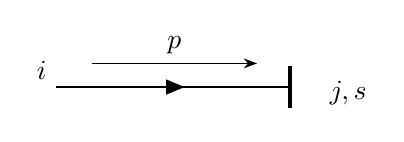
\begin{tikzpicture}
    \begin{feynman}
        % vertices
        \vertex (i) at (-1.5,0.0);
        \vertex (f) at (1.5,0.0);
        % edge labels
        \vertex [above left=-0.8pt and 0.0ptof i] (ti) {$i$};
        \vertex [above right=-10.0pt and 10.0pt of f] (tf) {$j, s$};
        % diagram
        \diagram* {
            (i)
            -- [fermion, momentum=\(p\),-{Bar[line width=1.5pt, width=15pt]}]
            (f)
            ,
        };
    \end{feynman}
\end{tikzpicture}
}
\quad
&:=
\quad
\delta\indices{^j_i}
\,
\bar{u}_s(p)
\\
\raisebox{-8pt}{
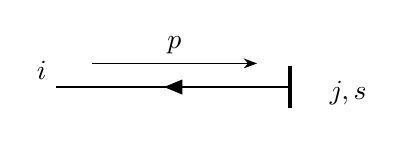
\begin{tikzpicture}
    \begin{feynman}
        % vertices
        \vertex (i) at (-1.5,0.0);
        \vertex (f) at (1.5,0.0);
        % edge labels
        \vertex [above left=-0.8pt and 0.0ptof i] (ti) {$i$};
        \vertex [above right=-10.0pt and 10.0pt of f] (tf) {$j, s$};
        % diagram
        \diagram* {
            (f)
            -- [fermion]
            (i)
            ,
            (i)
            -- [momentum=\(p\),-{Bar[line width=1.5pt, width=15pt]}]
            (f)
            ,
        };
    \end{feynman}
\end{tikzpicture}
}
\quad
&:=
\quad
\delta\indices{^i_j}
\,
v_s(p)
\,,
\end{align}
for outgoing, final state quarks and anti-quarks, respectively.
%
For initial-state quarks, \(\bar{u}_s(p)\) is replaced by \(u_s(p)\), while for initial-state anti-quarks, \(v_s(p)\) is replaced by \(\bar{v}_s(p)\).

\end{subequations}
\end{answer}

%%%%%%%%%%%%%%%%%%%%%%%%%%%%%%%%%%%%%%%%%%%%%%%%%%%%%%%%%%%%%%%

In this thesis, we will only be using the rules involving three-point vertices and external lines.
%
Other factors that will make consistent appearances in the discussions of this thesis are the \vocab{quadratic Casimirs} \(C_R\) and Dynkin indices \(T_R\) -- called \textit{group theory factors} -- defined by
\begin{align}
    \sum_a
    T^a_{(R)} T^a_{(R)}
    =:
    C_R
    1\!\!1_{\,(R)}
    \,,
\end{align}
where \(1\!\!1_{\,(R)}\) indicates the identity matrix in the representation \(R\), and
\begin{align}
    \Tr T^a_{(R)} T^b_{(R)}
    =:
    T_R \, \delta^{ab}
    \,.
\end{align}
In an unfortunate similarity of notation, the Dynkin index of the representation \(R\) is also denoted by a capital \(T\);
%
luckily, our notation is nonetheless unambiguous, as the Dynkin index \(T_R\) will never appear with a color index \(a\).

For the purposes of this thesis, we will use the standard normalization of the generators of SU(N) to obtain
\begin{align}
    C_A = N_c
    \qquad
    C_F = \frac{N_c^2 - 1}{2 N_c}
    \qquad
    T_F = \frac{1}{2}
    \,,
\end{align}
where \(A\) denotes the adjoint representation, under which gluons transform, and \(F\) denotes the fundamental representation, under which quarks transform.

\begin{exercise}
    \label{ex:group-theory-factors}
    Show that the group theory factors for the representation \(R\) are given by
    \begin{align}
        T_R \, \text{dim}(A)
        =
        C_R \, \text{dim}(R)
        \,,
    \end{align}
    where \(\text{dim}(R)\) indicates the dimension of the representation \(R\), and \(\text{dim}(A)\) -- the number of generators and the dimension of the adjoint representation -- is \(N_c^2 - 1\) for SU(\(N_c\)).

    What is the Dynkin index \(T_A\) of the adjoint representation?
\end{exercise}




\begin{definitionbox}{N\(^k\)LO Accuracy}{nklo}
    We say that results for (differential) cross sections/probability distributions, discussed in \Secs{scattering}{observables} respectively, are of leading-order accuracy (LO) if they involve no powers of \(g_s\):
    \begin{align}
        \text{LO cross section }
        \quad \leftrightarrow \quad
        \mathcal{O}(g_s^{0})
        \quad \leftrightarrow \quad
        \mathcal{O}(\alpha_s^0)
        \,,
    \end{align}
    next-to-leading order (NLO) if they involve two powers of \(g_s\):
    \begin{align}
        \text{NLO cross section }
        \quad \leftrightarrow \quad
        \mathcal{O}(g_s^{2})
        \quad \leftrightarrow \quad
        \mathcal{O}(\alpha_s^1)
        \,,
    \end{align}
    and N\(^k\)LO if they involve \(2k\) powers of \(g_s\):
    \begin{align}
        \text{N\(^k\)LO cross section }
        \quad \leftrightarrow \quad
        \mathcal{O}(g_s^{2k})
        \quad \leftrightarrow \quad
        \mathcal{O}(\alpha_s^k)
        \,.
    \end{align}

    Similarly, amplitudes are said to be LO at \(\mathcal{O}(g_s^0)\), NLO at \(\mathcal{O}(g_s)\), and N\(^k\)LO at \(\mathcal{O}(g_s^k)\).
\end{definitionbox}


\begin{example}
    \label{ex:gtogg-amplitude}
    A scattering amplitude to which we will return (at least implicitly) many times in the study of quarks, gluons, and jets, is the \(g \to gg\) \textit{splitting amplitude} describing the splitting of a single gluon into two gluons of lower energy.
    %
    Therefore, let us use the Feynman rules of \gls{qcd} to compute this amplitude of interest at NLO.

    Denoting the momentum of the incoming gluon as \(P\) and the outgoing gluons as \(k_1\) and \(k_2\) (to match later notation), the \(g \to g g\) splitting amplitude takes the form
    \begin{align}
        \raisebox{-26pt}{\scalebox{0.8}{
        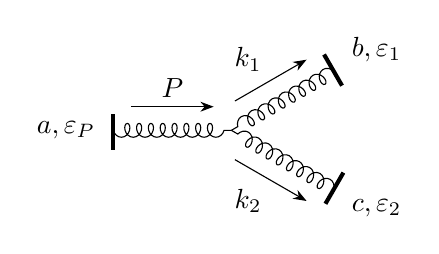
\begin{tikzpicture}
            \begin{feynman}
                % vertices
                \vertex (u) at (1.30,0.75);
                \vertex (l) at (-1.5,0);
                \vertex (r) at (1.30,-0.75);
                \vertex (cen) at (0,0);
                % edge labels
                \vertex [left=3.0ptof l] (tl) {$a, \varepsilon_P$};
                \vertex [above right=0.0pt and 3.0ptof u] (tu) {$b, \varepsilon_1$};
                \vertex [below right=0.0pt and 3.0pt of r] (tr) {$c,\varepsilon_2$};
                % diagram
                \diagram* {
                    (l)
                    -- [gluon, momentum=\(P\), postaction={decorate, decoration={markings, mark=at position 0 with {\draw[line width=1.5pt] (0,-7pt) -- (0,6pt);}}}]
                    (cen)
                    ,
                    (cen)
                    -- [opacity=0, -{Bar[line width=1.5pt, width=15pt]}]
                    (l)
                    ,
                    (u)
                    -- [gluon, postaction={decorate, decoration={markings, mark=at position 0 with {\draw[line width=1.5pt] (0,-7pt) -- (0,6pt);}}}]
                    (cen)
                    ,
                    (cen)
                    -- [momentum=\(k_1\), opacity=0]
                    (u)
                    ,
                    (r)
                    -- [gluon, postaction={decorate, decoration={markings, mark=at position 0 with {\draw[line width=1.5pt] (0,-7pt) -- (0,6pt);}}}]
                    (cen)
                    ,
                    (cen)
                    -- [momentum'=\(k_2\), opacity=0]
                    (r)
                };
            \end{feynman}
        \end{tikzpicture}
        }}
        =:
        \,\,\,
        \mathcal{M}_{g \to gg}
        \,.
    \end{align}
    Applying the Feynman rules, we find
    \begin{align}
        \mathcal{M}_{g \to gg}
        \,
        &=
        \,
        -g_s f^{abc}
        \,
        \varepsilon_P^\mu\, \varepsilon_1^{*\,\mu}\, \varepsilon_2^{*\,\mu}
        \le(
            (k_2 - k_1)_\mu \, g_{\nu\rho}
            + (-k_2 - P)_\nu \, g_{\mu\rho}
            + (P + k_1)_\rho \, g_{\mu\nu}
        \ri)
        \,.
    \end{align}
    Using \(k_1 \cdot \varepsilon_1^* = k_2 \cdot \varepsilon_2^* = P \cdot \varepsilon_P = 0\), we can instead write this as
    \begin{align}
        \mathcal{M}_{g \to gg}
        \,
        =
        \,
        2 g_s \le(
            k_1 \cdot \varepsilon_P
            \,\,
            {\scriptscriptstyle\times}
            \,\,
            \varepsilon_1^* \cdot \varepsilon_2^*
            +
            k_2 \cdot \varepsilon_1^*
            \,\,
            {\scriptscriptstyle\times}
            \,\,
            \varepsilon_P \cdot \varepsilon_2^*
            -
            k_1 \cdot \varepsilon_2^*
            \,\,
            {\scriptscriptstyle\times}
            \,\,
            \varepsilon_P \cdot \varepsilon_1^*
        \ri)
        \,.
    \end{align}

\end{example}

\begin{example}
    \label{ex:qtoqg-amplitude}
    Another important amplitude to which we will return many times (at least implicitly) is the \(q \to qg\) \textit{splitting amplitude}, describing the emission of a single gluon by a quark.
    %
    At NLO, denoting the momentum of the initial quark as \(P\), the final gluon as \(k_1\) and the final quark as \(k_2\), we may write
    \begin{align}
        \raisebox{-26pt}{\scalebox{0.8}{
        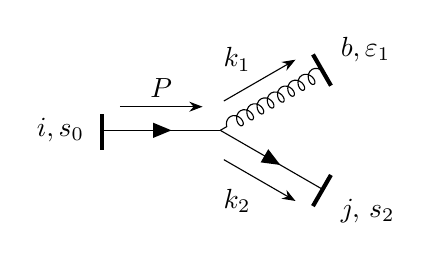
\begin{tikzpicture}
            \begin{feynman}
                % vertices
                \vertex (u) at (1.30,0.75);
                \vertex (l) at (-1.5,0);
                \vertex (r) at (1.30,-0.75);
                \vertex (cen) at (0,0);
                % edge labels
                \vertex [left=3.0ptof l] (tl) {$i, s_0$};
                \vertex [above right=0.0pt and 3.0ptof u] (tu) {$b, \varepsilon_1$};
                \vertex [below right=0.0pt and 3.0pt of r] (tr) {$j,\, s_2$};
                % diagram
                \diagram* {
                    (l)
                    -- [fermion, momentum=\(P\), postaction={decorate, decoration={markings, mark=at position 0 with {\draw[line width=1.5pt] (0,-7pt) -- (0,6pt);}}}]
                    (cen)
                    ,
                    (cen)
                    -- [opacity=0, -{Bar[line width=1.5pt, width=15pt]}]
                    (l)
                    ,
                    (u)
                    -- [gluon, postaction={decorate, decoration={markings, mark=at position 0 with {\draw[line width=1.5pt] (0,-7pt) -- (0,6pt);}}}]
                    (cen)
                    ,
                    (cen)
                    -- [momentum=\(k_1\), opacity=0]
                    (u)
                    ,
                    (cen)
                    -- [fermion, momentum'=\(k_2\), postaction={decorate, decoration={markings, mark=at position 1 with {\draw[line width=1.5pt] (0,-7pt) -- (0,6pt);}}}]
                    (r)
                };
            \end{feynman}
        \end{tikzpicture}
        }}
        =:
        \,\,\,
        \mathcal{M}_{q \to gq}
        \,.
    \end{align}
    Applying the Feynman rules,
    \begin{align}
        \mathcal{M}_{q \to gq}
        &=
        -i g_s
        \,\,
        \le(T^b\ri)\indices{^j_i}
        \,\,
        \varepsilon^{*\,\mu}_P
        \,\,\,
        \overline{u}_2 \,\gamma_\mu \, u_P
        \,,
    \end{align}
    where we use the shorthand \(u_i := u_{s_i}(k_i)\), \(i \in \{1,2\}\), and \(u_P := u_{s_0}(P)\).
\end{example}

\begin{exercise}
    \label{ex:gtoqq-amplitude}
    Show that the NLO amplitude for the splitting of a gluon of momentum \(P\) into a quark of momentum \(k_1\) and spin \(s_1\) and an anti-quark of momentum \(k_2\) and spin \(s_2\) is:
    \begin{align}
        \mathcal{M}_{g \to q \overline{q}}
        =
        -ig_s
        \,
        \le(T^a\ri)\indices{^j_i}
        \,\,
        \varepsilon_P^\mu
        \,\,\,
        \overline{u}_1 \, \gamma_\mu \, v_2
        \,.
    \end{align}
    In the notation above, does the quark or the anti-quark have momentum \(k_1\)?
    %
    Which external lines are labelled \(a\), \(i\), and \(j\)?
\end{exercise}



\remark{}{
    \gls{qcd} describes our universe in terms of quarks and gluons, while the universe we observe is composed of protons and neutrons.
    %
    The physics of hadrons such as protons and neutrons is more difficult to attack via analytic methods, and is often approached through the powerful lens of lattice \gls{qcd}.
    %
    There are also quantum field theories which are described in terms of hadronic fields alone, such as chiral effective field theory, but unfortunately these effective descriptions are not predictive at high energies.
}


\begin{definitionbox}{Hadron}{hadron}
    A \emph{\gls{hadron}} (from the Greek \(\acute{\alpha}\delta \rho \acute{o}\varsigma\), meaning ``stout'' or ``thick'') refers to a composite particle made of quarks which are bound together by and interact via the strong force, \gls{qcd}.
\end{definitionbox}

\remark{}{
    The most common hadrons are baryons (from \(\beta \alpha \rho \acute{\nu} \varsigma\), ``heavy'') such as the proton and neutron, which are composed of \(N_c = 3\) valence quarks, and mesons (from \(\mu\acute{\epsilon}\sigma o \varsigma\), ``intermediate'') such as pions or kaons, composed of a single quark and a single anti-quark.
}

An important feature of quantum field theory (and even of classical theories of statistical mechanics) is that the numbers describing the properties of the theory, \vocab{effective couplings}, change as a function of the properties of the properties of the physical problem under consideration.
%
For example, the probability that two particles scatter against one another changes in a \emph{surprising} way as the energy of the scattered particles is increased.
%
In particle physics applications, the properties of the physical problem under consideration are often (but not always) captured by a single energy scale, which we will call \(\mu\).

The derivation of the effective couplings describing a quantum field theory at different scales is achieved through renormalization methods available in standard textbooks on \gls{qft}.
%
For our purposes, it will be enough to note that the behavior of most effective \gls{qft} couplings of interest in particle physics can be captured by \textit{beta functions}:
%
\begin{definitionbox}{Beta Functions}{}
    The \vocab{beta function} for the coupling \(g\) is defined as
    \begin{align}
        \beta_g(g) = \frac{\dd\,\,g(\mu)}{\dd \ln\mu}
        \,,
    \end{align}
    where \(g(\mu)\) is an effective coupling governing interactions at the scale \(\mu\).
    %
    The behavior of \(g(\mu)\) as a function of \(\mu\), dictated by the functional form of \(\beta_g\), is called the \vocab{running} of \(g(\mu)\).
\end{definitionbox}

\remark{}{
    If \(g\) is a dimensional quantity, of mass dimension \(D\), called its \emph{engineering dimension}, we may expect that \(g\) scales as a function of \(\mu\) via \(g \propto \mu^D\), and thus that \(\beta_g(g) \overset{?}{=} D g\).
    %
    One often divides \(g\) by \(\mu^D\) to define a new coupling \(\tilde{g} = g / \mu^D\), with no mass dimension.
    %
    Na\"ively, and classically, we expect no running for \(\tilde{g}\):
    %
    \(\beta_{\tilde g}(\tilde g) \overset{?}{=} 0\).
    %
    If an explicit calculation yields \(\beta_{\tilde g} \neq 0\) however, then there is a breakdown of our classical intuition involving the scaling of \(g\) via engineering dimensions.
    %
    This occurs for the strong coupling constant in \gls{qcd}, and generically in quantum field theory (and statistical mechanics).
    %
    Since we expect classically that \(\beta_g(g)/g \overset{?}{=} D\) should yield the engineering dimension for \(g\), and that \(\beta_{\tilde g}/\tilde{g} = \beta_g(g)/g - D \overset{?}{=} 0\), the true value of \(\beta_{\tilde g}(\tilde{g}) / \tilde{g}\) is sometimes called the \emph{anomalous dimension} for \(g\), and is usually denoted \(\gamma_g\):
    \begin{align}
        \gamma_g
        :=
        \frac{\dd \, \ln \tilde{g}}{\dd \ln \mu}
        =
        \frac{\dd \, \ln g}{\dd \ln \mu}
        -
        D
        \,.
    \end{align}
    The scaling behavior of \gls{qft} operators, which also carry mass dimension, is often captured quantitatively by anomalous dimensions.
}

Particularly notable for the case of \gls{qcd} is the beta function for the Yang-Mills coupling \(g_s\), called the \textit{strong coupling constant}.
%
It is often parameterized in terms of perturbatively calculable coefficients as
\begin{align}
    \beta_{g_s}(g_s)
    =
    -g_s\,
    \sum_{n=0}^\infty \beta_n \le(\frac{g_s^2}{16\pi^2}\ri)^{n+1}
    \,,
\end{align}
or
\begin{align}
    \beta_{\alpha_s}(\alpha_s)
    =
    -2\alpha_s
    \sum_{n=0}^\infty \beta_n \le(\frac{\alpha_s}{4\pi}\ri)^{n+1}
\end{align}
where \(\alpha_s = g_s^2 / 4 \pi\) and the \(\beta_k\) are coefficients that can be captured by N\(^{k+1}\)LO computations.
%
This parameterization is used because the combination \(\alpha_s / 4\pi\) appears frequently in loop calculations.

In 1972-73, Gerard `t Hooft \cite{tHooft:1998qmr}, Hugh Politzer \cite{Politzer:1973fx}, and David Gross and Frank Wilczek \cite{Gross:1973ju} discovered through one-loop computations that the beta function of \gls{qcd} is negative.
%
In particular, with \(N_f\) quark flavors (i.e. up, down, charm, etc), the \glslink{accuracy}{NLO} running of the effective strong coupling constant is dictated by
\begin{align}
    \beta_0 = \frac{11}{3} C_A - \frac{4}{3} T_F N_f
    \,,
\end{align}
with the startling result that the effective coupling
\begin{align}
    \alpha_s(\mu)
    =
    \frac{\alpha_s(\mu_0)}{1 + \alpha_s(\mu_0) \beta_0 \ln\le(\mu / \mu_0\ri)/2\pi}
    \,,
\end{align}
\textit{decreases as a function of the energy scale} \(\mu\).
%
This was a dramatic discovery.
%
The beta functions of known quantum field theories, such as that of the electric coupling of QED, had all been positive%
\footnote{
    To my knowledge -- with the exception of \(\phi^3\)-theory, which has the undesirable feature that its energy is unbounded below, such that it has no perturbative vacuum state.
}

Even more dramatically, however, the effective value of \(g_s\) decreases to zero in the limit that scattered particles are given infinite energy, \(\mu \to \infty\).
%
This property of \gls{qcd} is called \vocab{asymptotic freedom}, and is crucial for the validity of our description of high-energy \gls{qcd} scattering processes in terms of quarks and gluons.
%
At high energies, quarks and gluons take the role of \textit{partons}:

\begin{definitionbox}{Parton}{parton}
    A \vocab{\gls{parton}} is a particle (e.g. defined by a field of a \gls{qft}) that is roughly non-interacting (and, for the purposes of this thesis, point-like).
\end{definitionbox}

\remark{}{
    In \gls{qcd}, partons are used to model the high-energy final states or the internal structures of composite particles such as protons and neutrons in high-energy scattering processes.
    %
    Partons need not be fundamental like the quarks and gluons of \gls{qcd}, however.
    %
    There are also parton models for strongly-interacting systems in dramatically different contexts -- most notably for the fractional quantum Hall effect in the context of condensed matter physics, in which the nearly-free ``particles'' are collective excitations of many electrons which nonetheless carry fractional charge \cite{jain2007composite}.
}


On the other hand, the effective value of the coupling \(\alpha_s\) increases at low energies, and eventually becomes so large that perturbative results cannot possibly be trusted.
%
This is already a hint of \emph{confinement}, the phenomenon in \gls{qcd} where quarks and gluons are permanently \textit{confined} within composite \textit{hadrons}, and cannot be isolated as free particles.%
\footnote{
    Nonetheless, asymptotic freedom loosely implies that, at high enough energies (or small enough length scales), quarks and gluons behave approximately freely.
    %
    Therefore, quarks and gluons are roughly de-confined in high energy environments such as the early stages of a hard process in a particle collision or the high-energy, high-density environment of the early universe.
}

\remark{confinement}{
    One argument that quarks must be confined is that the physical states of our universe must be gauge invariant in the framework of gauge theories like \gls{qcd}.
    %
    Other purely theoretical hints of\gls{confinement} include \textit{renormalons} in the quark propagator (see e.g. \cite{Altarelli:1995kz,Beneke:1998ui,Schindler:2023cww}), which indicate that quarks are not physical particles in that they do not correspond to poles of the \(S\)-matrix, and the theoretical considerations of the Gribov-Zwanziger model of \gls{qcd} \cite{Gribov:1977wm,Zwanziger:1988jt,Zwanziger:1989mf} that also indicate that \emph{gluons} do not correspond to poles of the \(S\)-matrix \cite{Zwanziger:1988jt} (see \Reff{Vandersickel:2012tz} for a review).
    %
    Additionally, extensive studies in lattice \gls{qcd} show that \gls{confinement} can be associated with the confining \textit{Cornell potential},
    \begin{equation}
        V(r) = -\frac{\kappa}{r} + \sigma r,
    \end{equation}
    between heavy quarks, where \( r \) is the distance between the quarks, \( \kappa \) is a constant associated with the Coulomb-like part of the quark potential, and \( \sigma \) is the string tension that causes the potential to increase linearly at large distances.
    %
    This linear increase in potential leads to the \gls{confinement} of quarks, as the energy required to separate them becomes arbitrarily large.
    %
    For light quarks, the potential eventually becomes constant due to \emph{string-breaking} effects, another beautiful tale which we will not have the opportunity to discuss.
    %
    \Reff{Greensite:2011zz} discusses the linearly-confining Cornell potential in the context of \gls{qcd}, and many other aspects of\gls{confinement}.
}


The results of high energy scattering experiments may be approximated through the use of perturbative \gls{qcd} calculations up to non-perturbative \emph{power corrections}, often of the form \((\LambdaQCD/Q)^n\), where \(n\) is a process-dependent real number and \(Q\) is a characteristic energy scale of the process.
%
We return to this point at a high level in \Sec{phd}.
%
For now, however, let us assume that partons are nearly free, and discuss what scattering in \gls{qft} really is.


\begin{exercise}
    \label{ex:lqcd-nonpert}
    Using the \gls{qcd} beta function, find the energy scale \(\mu = \LambdaQCD\) at which the strong coupling becomes infinite, \(\alpha_s(\LambdaQCD) := \infty\), in terms of the coupling \(\alpha_s := \alpha_s(\mu_0)\) given at a fixed initial scale \(\mu_0\).
    %
    Prove that \(\LambdaQCD\) cannot be expressed in terms of a power series in \(\alpha_s\), and that power corrections of the form \((\LambdaQCD/Q)^n\) are indeed non-perturbative.
\end{exercise}




% ---------------------------------------
\subsection{Principles of Scattering}
% ---------------------------------------
\label{sec:scattering}


The main tests of fundamental QFT are scattering experiments.
%
In \gls{qft}, scattering provides a framework for answering the question:
%
``What is the distribution of outgoing particles associated with a particular incoming state?''
%
Concretely, the framework of scattering can be developed if a \gls{qft} has a \textit{scattering description}:

\begin{definitionbox}{Scattering Description}{scattering-description}
    A \emph{\glslink{scattering}{scattering description}} of a \gls{qft} is a description of the states of the \gls{qft} at \(t = \pm \infty\) -- called \textit{in-} and \textit{out-states} -- in terms of the known eigenstates of a ``free'' Hamiltonian.
    %
    The in- and out-states have the property that they have the properties of ``free'' particle states at \(t = \pm\infty\).

    \vspace{7pt}
    \hrule
    \vspace{7pt}

    A \vocab{scattering description} for a quantum-mechanical theory with Hamiltonian \(H\) is a complete set of \textit{in-states}, \(\{\ket{\alpha}_+\}\), associated with the Hilbert space at \(t = -\infty\), and \textit{out-states}, \(\{\ket{\alpha}_-\}\), associated with \(t = +\infty\), together with the eigenstates \(\{\ket{\alpha}_0\}\) of a Hamiltonian \(H_0\) -- often called the ``\textit{free Hamiltonian}'':
    \begin{align}
        H \ket{\alpha}_\pm = E_\alpha \ket{\alpha}_\pm
        \qquad
        H_0 \ket{\alpha}_0 = E_\alpha \ket{\alpha}_0
        \,,
    \end{align}
    where the eigenvalues \(E_\alpha\) of the free Hamiltonian are known, and the in- and out-states behave like free-particle eigenstates at early and late times, respectively:
    \begin{align}
        \label{eq:scattering-states}
        \lim_{t \to \mp\infty}
        \int \dd \alpha \int e^{-i E_\alpha t}
        g(\alpha) \ket{\alpha}_\pm
        =
        \dd \alpha \int e^{-i E_\alpha t}
        g(\alpha) \ket{\alpha}_0
        \,,
    \end{align}
    where \(g(\alpha)\), known as a \vocab{wavepacket}, specifies a smooth, normalizable superposition of energy eigenstates.
\end{definitionbox}

\remark{}{
    This precise definition, a reformulation of the definitions given in Chapter 3.1 of Weinberg's \underline{The Theory of Quantum Fields, Volume I} \cite{Weinberg:1995mt}, is taken from \href{https://www.mit.edu/~harlow/HarlowQFT1.pdf\#page=101}{Chapter 8.3 of Daniel Harlow's exceptional notes on quantum field theory} \cite{Harlow:2024zz}.
    %
    The basics of scattering theory in this framing discussed in depth in Prof. Harlow's notes.
    %
    I can also recommend the complementary presentations of \Reffs{Srednicki:2007qs,Schwartz:2014sze}.
}

\remark{}{
    The defining feature of the scattering description of a \gls{qft} given in \Eq{scattering-states} is often re-written as
    \begin{align}
        \label{eq:interaction-evolution}
        \lim_{t \to \mp \infty}
        \overline{T}\le(e^{i \int^{\mp\infty} H_0 \dd t}\ri)
        T\le(e^{-i \int^{\mp\infty} H \dd t}\ri)
        \ket{\alpha}_\pm
        =:
        \lim_{t \to \mp \infty}
        U_I(t)
        \ket{\alpha}_\pm
        =
        \ket{\alpha}_0
        \,,
    \end{align}
    where \(T\) and \(\overline{T}\) indicate time-ordering and anti-time-ordering prescriptions, respectively.
    %
    The \textit{interaction picture evolution operator} of \Eq{interaction-evolution} is meaningful only when acting on smooth superpositions of energy eigenstates.
    %
    \Eq{interaction-evolution} is often written as an evolution of operators rather than states via:
    \begin{align}
        \label{eq:interaction-picture}
        \varphi(x, t)
        =
        U_I^\dagger(t) e^{i H_0 t} \varphi(x, 0) e^{-i H_0 t} U_I(t)
        =:
        U_I^\dagger(t) \varphi_I(x, t) U_I(t)
        \,,
    \end{align}
    where we have now assumed that \(H_0\) is time independent.
    %
    \(\phi_I(x, t)\) is referred to as an operator in the \vocab{interaction picture}, which evolves only with the free Hamiltonian (rather than with the full Hamiltonian, as in the Heisenberg picture).
    %
    The interaction picture is an important tool in \gls{qft} which allows us to compute amplitudes and correlation functions using the technology of free fields.
    %
    A wonderful introduction to the mechanics of the interaction picture can be found in \href{https://web.physics.ucsb.edu/~mark/ms-qft-DRAFT.pdf\#page=84}{Mark Srendicki's \underline{Quantum Field Theory}, Problem 9.5}.
}

\remark{}{
    The existence of scattering descriptions/the interaction picture of \gls{qft} is technically ruled out by a \href{https://en.wikipedia.org/wiki/Haag\%27s_theorem}{\textit{theorem of Rudolf Haag}}, which states roughly that free and interacting quantum field theories have necessarily different/incompatible Hilbert spaces.
    %
    The Haag-Ruelle scattering theory \cite{Haag:1958vt,Ruelle:1963ee} overcomes some but not all of these technical difficulties.
    %
    Remaining are difficulties involving massless particles and bound states, both of which are relevant for the topics of this thesis.
    %
    Nonetheless, we will push forward with the popular and wildly successful description of particle scattering exposited in this section.
}


The scattering definition of a \gls{qft} leads us to an extremely important quantity:
%
the scattering matrix, or \(S\)-matrix:

\begin{definitionbox}{\(S\)-matrix}{s-matrix}
    The \vocab{\(S\)-matrix} of a \gls{qft} is the overlap of the in- and out-states:
    \begin{align}
        S_{\beta \alpha}
        =
        {}_-\!\braket{\beta}{\alpha}_+
        \,.
    \end{align}
    The \(S\)-matrix provides a quantitative answer to the question:
    %
    ``If I begin with a state \(\ket{\alpha}_+\) at \(t = -\infty\), what distribution of states will I see at \(t = +\infty\)?''

    \vspace{7pt}
    \hrule
    \vspace{7pt}

    The \(S\)-matrix has a ``trivial'' part \(S_{\beta\alpha} \supset \delta(\beta - \alpha)\) which reflects the possibility of no scattering.
    %
    The possibility of non-trivial scattering is contained within the connected component of what is conventionally called \(\mathcal{M}\), conventionally defined by computing \(S_{\beta\alpha}\) in terms of states \(\ket{\beta}_-\) and \(\ket{\alpha}_+\) which are assumed to be momentum eigenstates:
    \begin{align}
        S_{\beta \alpha}
        =
        \delta(\beta - \alpha)
        +
        i\,
        \le(2\pi\ri)^d \delta^{(d)}\le(p_\beta - p_\alpha\ri)
        \mathcal{M}_{\beta\alpha}
        \,.
    \end{align}

    \underline{The \(\mathcal{M}_{\beta\alpha}\) are called \vocab{\gls{scattering} amplitudes}.}
\end{definitionbox}

We will now motivate the definition of the cross section with heuristic arguments;
%
a full treatment can be found in many resources, including \Reffs{Peskin:1995ev,Srednicki:2007qs,Schwartz:2014sze}.

We are interested in comparing theoretical predictions for scattering to experimental results.
%
Therefore, we want to know the probability to obtain an outgoing state in a specific region of outgoing phase space \(\Phi_\text{out}\) given our initial scattering state.

Ignoring the possibility of no scattering, and beginning in a properly normalized state \(\ket{\alpha}\), we follow the rule that probabilities are given by amplitudes squared to na\"ively write
\begin{align}
    \mathbb{P}\le(\alpha \to \Phi_\text{out}\ri)
    =
    \int_{\beta \in \Phi_\text{out}}
    \dd N_\beta
    \le(2 \pi\ri)^{2d}
    \le(\delta^{(d)}\le(p_\beta - p_\alpha\ri)\ri)^2
    \abs{\mathcal{M}_{\beta\alpha}}^2
    \,,
\end{align}
where \(\dd N_\beta\) is  number of states available in a phase space window around the state \(\ket{\beta}\);
%
it will be better defined when we work in a (momentum-eigenstate) basis.
%
We are left with an expression involving the ill-defined square of a delta function.
%
Now we use our physical intuition.
%
In finite volume/time, \((2\pi)^d \delta^{(d)}(0)\) can be replaced by \(V T\), where \(V\) is the finite volume of space and \(T\) is the finite extent of time.
%
Therefore, we can write the well-defined expression
\begin{align}
    \label{eq:probability-propertly-normalized}
    \frac{1}{V\,T}
    \,
    \mathbb{P}\le(\alpha \to \Phi_\text{out}\ri)
    =
    \int_{\Phi_\text{out}}
    \dd \beta
    \le(2 \pi\ri)^{d}
    \delta^{(d)}\le(p_\beta - p_\alpha\ri)
    \abs{\mathcal{M}_{\beta\alpha}}^2
    \,.
\end{align}

\Eq{probability-propertly-normalized} holds in the case that \(\ket{\alpha}\) indicates a properly-normalized state;
%
however, the free momentum eigenstates of \gls{qft} (much like those of non-relativistic quantum mechanics) are not properly normalized.
%
For improperly-normalized states, we must instead write
\begin{align}
    \label{eq:probability-not-normalized}
    \frac{1}{V\,T}
    \,
    \mathbb{P}\le(\alpha \to \Phi_\text{out}\ri)
    =
    \int_{\Phi_\text{out}}
    \dd \beta
    \le(2 \pi\ri)^{d}
    \delta^{(d)}\le(p_\beta - p_\alpha\ri)
    \abs{\mathcal{M}_{\beta\alpha}}^2
    \frac{1}{\braket{\alpha}{\alpha}\,\braket{\beta}{\beta}}
    \,.
\end{align}

When \(\alpha\) and \(\beta\) denote (improperly normalized) momentum eigenstates, we write
\begin{align}
    \dd N_\beta = \prod_{j \in \beta}\le(V \, \frac{\dd^{d-1} k_j}{(2\pi)^{d-1}}\ri)
    \,,
\end{align}
for the number of states available to \(\ket{\beta}\) in the phase space window defined by \(\dd^{d-1} k_j\).
%
The Lorentz-invariant normalization for momentum eigenstates is derived in introductory textbooks on \gls{qft}%
\footnote{
    See, for example, Eqs. (5.10) through (5.21) in Matthew Schwartz' \underline{Quantum Field Theory and the Standard Model} \cite{Schwartz:2014sze}.
};
%
for single-particle states, it takes the form \(\braket{p}{k} = 2 E_p (2\pi)^{d-1} \delta^{(d-1)}\le(\vec{p} - \vec{k}\ri)\), and therefore, in finite volume, \(\braket{p}{p} = 2 E_p \, V\).
%
If \(\ket{\psi_n}\) denotes an \(n\) particle state composed of momentum eigenstates, in the non-degenerate limit for which none of the quantum numbers of the \(n\) particles in \(\ket{\psi_n}\) are exactly the same, then,
\begin{align}
    \braket{\psi_n}{\psi_n}
    =
    \prod_{j = 1}^n \le(2 \, V\, E_j\ri)
    \,.
\end{align}

Defining the \vocab{outgoing Lorentz-invariant phase space measure},
\begin{align}
   \dd\Phi_\beta(\alpha)
   =
   \le(2\pi\ri)^d \delta^{(d)}\le(p_\beta - p_\alpha\ri)
   \frac{\dd N_\beta}{\braket{\beta}{\beta}}
   =
   \le(2\pi\ri)^d \delta^{(d)}\le(p_\beta - p_\alpha\ri)
   \prod_{j \in \beta}
    \frac{\dd^{d-1} k_j}{(2\pi)^{d-1}\, 2 E_j}
   \,,
\end{align}
and taking the additional normalization factors into account, we can re-write \Eq{probability-not-normalized}, in the \textit{differential} form
\begin{align}
    \frac{V^{N_\alpha - 1}}{T}
    \dd \mathbb{P}\le(\alpha \to \beta\ri)
    =
    \prod_{i \in \alpha} \frac{1}{2 E_i}
    \,
    \abs{\mathcal{M}_{\beta\alpha}}^2
    \,
    \dd \Phi_\beta(\alpha)
    \,.
\end{align}
The \vocab{differential rate} for the process \(\alpha \to \beta\) is then
\begin{align}
    \label{eq:differential-rate}
    \frac{1}{T}
    \dd \mathbb{P}\le(\alpha \to \beta\ri)
    :=
    \dd \Gamma\le(\alpha \to \beta\ri)
    =
    V^{1 - N_{\alpha}}
    \prod_{i \in \alpha} \frac{1}{2 E_i}
    \,
    \abs{\mathcal{M}_{\beta\alpha}}^2
    \,
    \dd \Phi_\beta(\alpha)
    \,.
\end{align}


\begin{exercise}
    \label{ex:lorentz-invariant-phase-space}

    Show that the phase space factor for a single final-state particle can be written in the manifestly (orthocronous) Lorentz invariant form
    \begin{align}
        \frac{\dd^{d-1} k}{\le(2\pi\ri)^{d-1} 2 E_k}
        =
        \int
        \frac{\dd^d k}{\le(2\pi\ri)^d}
        \Theta(k^0 > 0) \delta\le(k^2 - m^2\ri)
        \,,
    \end{align}
    where the integral of the right-hand-side is done over \(k^0\) (and is often left out in writing).

    To simplify formal expressions, the definition
    \begin{align}
        \delta_+\le(k^2 - m^2\ri)
        :=
        \Theta\le(k^0 > 0\ri)\,\delta\le(k^2 - m^2\ri)
        \,,
    \end{align}
    is often made.
\end{exercise}


Finally, we return to experimental concerns.
%
In a scattering experiment, for which \(N_\alpha = 2\), we will need the results from many collisions in order to extract meaningful results about our microscopic universe through the scientific method.
%
Therefore, let us assume that we scatter an \textit{infinite} number of particles, slamming together particles of number density \(\rho_\alpha = 1/V\) at relative velocity \(u_{\alpha}\) with the \vocab{particle-number flux}
\begin{align}
    f_\alpha = u_\alpha \rho_\alpha
    \,.
\end{align}

Dividing both side of the differential rate of \Eq{differential-rate} by the flux, we obtain what is called the \textit{cross section}:

\begin{definitionbox}{Cross Section}{}
    The \emph{\gls{xsec}} for the process \(\alpha \to \beta\) is the rate of scattering per incoming particle-number flux for the process \(\alpha \to \beta\).

    \vspace{7pt}
    \hrule
    \vspace{7pt}

    The \vocab{differential cross section} for the process \(\alpha \to \beta\), where \(\alpha\) is an incoming state describing two particles (\(N_\alpha = 2\)), is given by
    \begin{align}
        \label{eq:differential-xsec}
        \frac{1}{T\,f_\alpha}
        \dd \mathbb{P}\le(\alpha \to \beta\ri)
        :=
        \dd \sigma\le(\alpha \to \beta\ri)
        =
        \frac{1}{u_\alpha}
        \frac{1}{4 E_{p_1} E_{p_2}}
        \dd \Phi_\beta(\alpha)
        \abs{\mathcal{M}_{\beta\alpha}}^2
        \,.
    \end{align}

    The \vocab{total (inclusive) cross section} for the process \(\alpha \to \Phi_\text{out}\) in which an incoming state \(\alpha\) scatters into the phase space \(\Phi_\text{out}\) is
    \begin{align}
        \label{eq:total-xsec}
        \SumInt_{\beta \in \Phi_\text{out}}
        \dd \sigma\le(\alpha \to \beta\ri)
        =
        \frac{1}{u_\alpha}
        \frac{1}{4 E_{p_1} E_{p_2}}
        \SumInt_{\beta \in \Phi_\text{out}}
        \dd \Phi_\beta(\alpha)
        \,
        \abs{\mathcal{M}_{\beta\alpha}}^2
        \,,
    \end{align}
    where \(\SumInt\) indicates the possible sum over discrete labels of \(\beta\) (such as the number of outgoing particles \(N_\beta\)) as well as the integral the phase space of \(\beta\) for each set of discrete labels for \(\beta\) (e.g. the integral over the differential phase space for two, three, or four particles, etc.).
\end{definitionbox}

\remark{}{
    In the center of mass frame, the relative velocity between two incoming particles labelled 1 and 2 takes the form
    \begin{align}
        u_\alpha^{\text{(c.o.m)}}
        =
        \abs{\frac{\vec{p}_1}{E_1} - \frac{\vec{p}_2}{E_2}}
        \,.
    \end{align}
    When the particles have identical mass, we have
    \begin{align}
        u_\alpha^{\text{(c.o.m)}}(m)
        =
        2 \sqrt{1 - \frac{2m}{\sqrt{s}}}
        \,,
    \end{align}
    where \(\sqrt{s}\) is the center-of-mass energy.
    %
    Notably \(u_\alpha = 2\) in the center-of-mass frame in the limit of infinite energy or of zero mass -- the cases involved in the explicit calculations presented in this thesis.
}



%\begin{exercise}
%    \label{ex:two-to-two-xsec}
%    Consider the case of 2-to-2 scattering, with momenta \(p_1 + p_2 \to k_1 + k_2\) in the center-of-mass frame.

%    Show that once momentum conservation is taken into account, integrals over the final-state Lorentz-invariant phase space can be expressed in terms of angles and momenta in the center-of-mass frame by
%%
%{fix for \(d\) dimensions, missing initial-state factors}
%    \begin{align}
%        \int \dd\Phi_2
%        F(\Phi_2)
%        =
%        \frac{}{}
%        \frac{\abs{\vec{k}_1}}{16 \pi^2 \sqrt{s}}
%        \int \dd\Omega_{d-2}
%        \,\,
%        F(\Phi_2)\Big|_\Omega
%        \,,
%    \end{align}
%    where \(\sqrt{s}\) is the center-of-mass energy of the scattering, and \(F(\Phi_2)\Big|_\Omega\) indicates the function \(F(\Phi_2)\) evaluated in a region of final-state phase space in which momentum is conserved and the two outgoing particles move along an axis determined in the solid angle \(\dd \Omega_{d-2}\), defining a point on the \(d-2\)-dimensional unit sphere.

%    Conclude that, for 2-to-2 scattering in the high energy limit (i.e. with massless particles) in \(d = 4-2\epsilon\) dimensions,
%%
%{fix for \(d\) dimensions, missing initial-state factors}
%    \begin{align}
%        \int
%        \dd \sigma F(\Phi_2)
%        =
%        \frac{1}{64\pi^2 s}
%        \int \dd\Omega_{d-2} F(\Phi_2)\Big|_\Omega
%        \,.
%    \end{align}


%    \vspace{7pt}
%    \hrule
%    \vspace{7pt}

%    \texttt{(Hint:)}
%    This is shown for \(d=4\) in Matthew Schwartz' \textit{Quantum Field Theory and the Standard Model}, Chapter 5 \cite{Schwartz:2014sze};
%    %
%    the analogous statement for general \(d =: 4-2\epsilon\) follows a similar proof.
%    %
%    See also \Reff{Giele:1991vf}.
%\end{exercise}


% ---------------------------------------
\subsection{Collider Observables}
% ---------------------------------------
\label{sec:observables}

\epigraph{
    the art of jet substructure is in the construction of observables
}{
    Andrew Larkoski, \textit{QCD Masterclass Lectures on Jet Physics and Machine Learning} \cite{Larkoski:2024uoc}
}

To gain actual understanding of our universe from the theoretical calculations involved in scattering, we need to design experimentally-addressable ways of extracting information from sets of outgoing momenta.
%
To do so, we will introduce the concept of \textit{collider observables}.
%
With collider observables in hand, we will be able to compare experimental results for the averages or distributions of these observables to the theoretical predictions obtained with pQCD.

\begin{definitionbox}{Collider Observable}{observable}
    A \emph{\gls{observable}} is a map which takes in a set of outgoing momenta of a collision event, and returns a simple representation of the information contained in the collision.

    \vspace{7pt}
    \hrule
    \vspace{7pt}

    In the context of collider physics, a \vocab{collider observable} is a map from a set of any number of outgoing momenta to a predefined \textit{target space} \(T\):
    \begin{align}
        X: S \to T
        \,,
    \end{align}
    where \(S\) is the set of all possible outgoing momenta:
    \begin{align}
        S &= \bigcup_{n=0}^\infty \le\{
            (p_1, \,\dots,\, p_n)
            \,\,
            |
            \,\,
            E_i > 0 \text{ for all } 1 \leq i \leq n
        \ri\}
        \,.
    \end{align}
\end{definitionbox}
Many common collider observables are \textit{real-valued}, meaning that their target space is the set of real numbers, \(T = \mathbb{R}\).
%
One important example is the mass of certain sets of outgoing particles (\textit{jets}, discussed in the next chapter);
%
masses, and the closely related \glspl{angularity}, and \glslink{gecf}{Generalized Energy Correlation Functions (GECFs)}, will play a central role in our discussion of the internal structure of particles and, in the next chapter, the jets that represent them.
\begin{itemize}
    \item
    \vocab{\Glspl{angularity}:}

    For the purposes of this thesis,%
    \footnote{
        Angularities are often defined in terms of transverse momenta in the context of proton-proton collisions, since experimental detectors in proton-proton collisions have significantly better resolution in measurements of the transverse momenta of particles than in measurements of their energies.
        %
        Nonetheless, in our theoretical analyses we will consider collections of particles -- jets -- that are \emph{central} (with a rapidity \(y = 0\) -- meaning that they are approximately perpendicular to the beams of colliding protons) and narrow (\(R_0 \ll 1\);
        %
        under these assumptions, the angularities take the stated form.
    }
    %
    the \emph{angularity} associated with a group of \(M\) particles is
    \begin{equation}
        e_{\varsigma}
        \simeq
        \sum_{i=1}^M
        z_i \left(\frac{\theta_{i}}{R_0}\right)^\varsigma
        \label{eq:angularitydefn_lo}
        \,,
    \end{equation}
    where the sum is over particles in the jet, \(z_i = E_i / E_\text{tot}\) represents the fraction of energy carried by particle \(i\), \(\theta_i\) is the angle between the momentum of particle \(i\) and an \textit{axis} associated with the collection of particles (in \Chap{jets}, the axis will correspond to the direction of a jet's momentum), and \(R_0\) indicates an angular scale (in \Chap{jets}, the jet radius).

    \item
    \vocab{\glslink{gecf}{Generalized Energy Correlation Functions (GECFs)}:}

    For the purposes of this thesis,%
    \footnote{Again, under the assumption that we are using central and narrow jets.}
    %
    we may write the ECFs in the form
    \begin{equation}
        C_1^{(\varsigma)}
        \simeq
        \frac{1}{2}\sum_{i=1}^M\sum_{j=1}^M
        z_i z_j \left(\frac{\theta_{ij}}{R_0}\right)^\varsigma
        \label{eq:GECFdefn_lo}
        ,
    \end{equation}
    where \(\theta_{ij}\) indicates the angle between particles \(i\) and \(j\).
    %
    \Eq{GECFdefn_lo} holds up to non-singular corrections in powers of the jet radius, which we neglect \cite{Larkoski:2014wba}.
\end{itemize}
%
These observables are closely related to the more intuitive jet mass -- \(m^2 / p_T^2 \approx e_2 \approx C_1^{(2)}\) -- with a simple form that can be represented as sums on emissions within a jet.
%
This \textit{additive} property is emphasized in \Sec{ll-substructure-diagrams}, where it is especially useful in computing the all-orders structures of their distributions.

\remark{}{
    There are important collider observables for which \(T \neq \mathbb{R}\).
    %
    In \Chap{grooming}, we show how \gls{jet-grooming} algorithms act on the set of outgoing momenta \(S\) and return a \textit{new} set of outgoing momenta in \(S\);
    %
    grooming algorithms are collider observables for which the target space is \(T = S\).
    %
    In \Chap{ewocs}, we will consider \glslink{ewoc}{energy-weighted observable correlations}, observables for which the target space \(T\) is a space of generalized functions (or \textit{distributions}).
    %
    The topological properties of these exotic target spaces will play a role in our later attempts to define continuous jet substructure observables which are insensitive to low-energy pollution (low energy pollution is discussed in \App{pollution-models}).
}


\remark{}{
    In quantum mechanics, observables are often defined as hermitian operators.
    %
    The collider observables we define above can be cast in a comparable way, but are more convenient for the purposes of this thesis.
}



Given a collider observable and a set of scattering outcomes, we can define the \textit{differential cross section} and \textit{probability distribution} associated with the collider observable.
%
These will be the main tools used in this thesis to explore the fundamental nature of our universe:

\begin{definitionbox}{Distribution of a Collider Observable}{}
Given a set of outgoing states defined by the phase space \(\Phi_\text{out}\) the \vocab{probability distribution of a} (real-valued) \vocab{collider observable} \(X\) can be obtained by taking the differential cross section for the collider observable,
    \begin{align}
        \label{eq:diff-xsec-for-x}
        \frac{\dd \sigma\le(\alpha \to \Phi_\text{out}\ri)}{\dd X}(x)
        =
        \frac{1}{u_\alpha\, 4 E_{p_1} E_{p_2}}
        \SumInt_{\beta \in \Phi_\text{out}}
        \dd \Phi_\beta(\alpha)
        \,
        \abs{\mathcal{M}_{\beta\alpha}}^2
        \,\,
        \delta\le(X(\beta) - x\ri)
        \\
        \int \dd \sigma(\alpha \to \Phi_{\text{out}})
        \,
        \delta\le(X(\beta) - x\ri)
        \,,
    \end{align}
    and dividing by the total cross section for \(\alpha \to \Phi_\text{out}\):
    \begin{align}
        \rho_X(x)
        :=
        \frac{\dd \mathbb{P}}{\dd X}(x)
        :=
        \frac{1}{\sigma\le(\alpha \to \Phi_\text{out}\ri)}
        \frac{\dd \sigma\le(\alpha \to \Phi_\text{out}\ri)}{\dd X}(x)
        \,.
    \end{align}


    The key new feature of \Eq{diff-xsec-for-x} is the delta function \(\delta\le(X(\beta) - x\ri)\), which enforces that contributions to \(\dd\sigma/\dd X(x)\) only come from states \(\beta\) for which \(X\) evaluated on \(\beta\) gives the number \(x\).
\end{definitionbox}

\remark{}{
    By construction, the probability distribution \(\rho_X\) integrates to one:
    \begin{align}
        \int \dd x
        \,
        \rho_X(x)
        =
        \frac{\sigma\le(\alpha \to \Phi_\text{\rm out}\ri)}
            {\sigma\le(\alpha \to \Phi_\text{\rm out}\ri)}
        =
        1
        \,.
    \end{align}
}


\begin{answer}
    We have therefore reduced the problem of designing theoretical predictions for the outcomes of collider experiments to calculations of the \(\mathcal{M}_{\alpha\beta}\):
    %
    the non-trivial and connected pieces of the \(S\)-matrix.

    \textbf{Calculations of \(M_{\alpha\beta}\) can be converted into theoretical predictions for probability distributions of collider observables in collision experiments.}
\end{answer}

\remark{}{
    In most collider contexts -- all with which I am familiar -- experimental detectors are sensitive to the momenta but not the spins of final state particles.
    %
    Furthermore, it is common for the colliding particles to be arranged in \textit{unpolarized beams}, such that all possible spin states of the initial particles occur with equal probability.
    %
    Therefore, to make physical predictions, we will often \textit{average over initial state labels} -- including spin or color -- and \textit{sum over final state labels} of the square of a scattering amplitude.
    %
    We will denote this common procedure by a ``barred'' sum.
    %
    Schematically,
    \begin{align}
        \overline{\sum}
        \abs{\mathcal{M}(\alpha \to \beta)}^2
        \,\,
        =
        \,\,
        \le(
        \prod_{i \in \alpha} \frac{1}{N_i}
        \ri)
        \,\,
        \sum_{\{\ell_i\}_{i \in \alpha}}
        \,
        \sum_{\{\ell_j\}_{j \in \beta}}
        \,
        \abs{\mathcal{M}\le(\alpha,\{\ell_i\}\,\to\,\beta,\{\ell_j\}\ri)}^2
        \,,
    \end{align}
    where \(\ell_i\) and \(\ell_j\) denote the possible initial state spins, colors, etc of the initial- and final-state particles, respectively, and \(N_i\) denotes the total number of possible distinct labels for particle \(i\).
    %
    For example, for a massive particle \(i\) of spin \(s_i\) and no other quantum numbers, \(N_i = 2 s_i + 1\).
    %
    However, it is important to note that massless spin-1 particles still have only two polarizations;
    %
    a massless photon is associated with \(N_i = 2\).
}

\begin{exercise}
    Why do we consider spin sums over amplitudes squared, rather than the spin sums of amplitudes themselves?
\end{exercise}



\begin{exercise}
    \label{ex:squared-amplitudes}
    Use Lorentz invariance to argue that the spin summed squares of the three-point amplitudes massless \gls{qcd} -- in Examples~\ref{ex:gtogg-amplitude} and \ref{ex:qtoqg-amplitude} and Exercise \ref{ex:gtoqq-amplitude} -- all vanish on-shell.
\end{exercise}


The relationship between measurable probability distributions and theoretical \(S\)-matrix elements is our first step towards understanding particle collisions.
%
However, it is not the end of the story.
%
We have yet to deal with the infamous infinities of \gls{qft} -- poorly-defined artifacts of calculations of \(\mathcal{M}_{\beta\alpha}\), which are revealed by singular features of both quantum-mechanical scattering amplitudes and integrals over the classical phase space of outgoing massless particles.

We will learn about the seemingly problematic infinities of \gls{qft} in \Secs{irc-safety}{splitting-functions} where we will discuss, unfortunately somewhat briefly, how they are actually necessary components of the quantum ecosystem.
%
The infinities of \gls{qft} can be described as either \vocab{infra-red (IR)}, emerging from integrals over regions of phase space with miniscule momenta, or \vocab{ultraviolet (UV)}, emerging from regions of phase space with enormous momenta.
%
The IR infinites of \gls{qft} hint at the intricate and unknowable properties of low-energy radiation, and will play the more dominant role in this thesis.
%
The UV infinities of \gls{qft} reveal the structure of renormalization -- a feature whose modern understanding was pioneered by Kenneth Wilson, earning him the 1982 Nobel Prize.

There are several ways of addressing the seemingly infinite predictions of \gls{qft} due to UV and IR divergences.
%
The technically simplest technique (and thereby the most practiced) is that of \vocab{dimensional regularization}:
%
the technique of using the formal properties of integrals to ``pretend'' we are in a complex number of spacetime dimensions
\begin{align}
    d = 4 - 2\epsilon \neq 3 + 1
    \,,
\end{align}
in order to produce formally convergent integrals (via an axiomatically well-defined analytic continuation in \(\epsilon\) -- see \Reff{Collins:1984xc}) which may be evaluated to produce finite theoretical predictions for scattering amplitudes.
%
When used with care, dimensional regularization removes the divergences emerging from both quantum corrections to scattering amplitudes -- called \textit{loop corrections} -- and integrations over the outgoing phase space of massless particles.
%
A more general treatment of both types of divergences using dimensional regularization is a staple of modern texts on quantum field theory;
%
for a textbook focused on development of systematic technology and applications for dimensional regularization, see \Reff{Collins:1984xc}.


Importantly, the IR divergences of standard \glspl{qft} (including the \gls{sm} and \gls{qcd}) cancel between quantum mechanical corrections (loop integrals) and corrections due to real emissions (integrals over classical phase space) in the calculation of inclusive cross sections.
%
The proof of this result, called the \vocab{Kinoshita-Lee-Nauenberg (KLN) theorem} \cite{Kinoshita:1962ur,Lee:1964is} (see also \Reff{Frye:2018xjj}), is \textit{far} beyond the scope of this thesis;
%
it is a giant on whose shoulders we will stand moving forward:

\begin{theorembox}{Kinoshita-Lee-Nauenberg (KLN) Theorem}{kln}
    The sum/integral of the square of the \(S\)-matrix over \vocab{degenerate states},
    \begin{align}
        \SumInt_{\alpha \in D(E)}
        \dd \alpha
        \SumInt_{\beta \in  D(E)}
        \dd \beta
        \,\,\,
        S^\dagger_{\gamma \beta}
        \,
        S_{\beta \alpha}
        \,,
    \end{align}
    where \(D(E)\) indicates a set of degenerate states all with energy \(E\), \vocab{is free of IR divergences}.
    %
    Note that \(E = E_\alpha = E_\beta\) by energy conservation.
\end{theorembox}
%
The key cancellation ensuring the validity of the KLN theorem in \gls{qcd}, and in \glspl{qft} involving massless particles, is between IR loop divergences of \(N\)-particle amplitudes and the IR divergences from integrals over \(N+1\) particle phase space.
%
The KLN theorem motivates the criterion of \glslink{irc-safety}{infra-red and collinear (IRC) safe} collider \glspl{observable}, which exhibit well-behaved perturbative properties, discussed in \Sec{irc-safety}.

\remark{faddeev-kulish}{
    The Faddeev-Kulish (FK) formalism for dressed, gauge invariant scattering \cite{Kulish:1970ut}, inspired by the preliminary work of P.A.M. Dirac \cite{Dirac:1955uv} and the later work of \Reff{Chung:1965zza}, offers a complementary perspective on IR finiteness (see also \Reff{Contopanagos:1991yb} for more developments on the KLN perspective).
    %
    The FK formalism operates under the assumption that infra-red finiteness may be ensured by working with appropriately defined initial and final states involving \vocab{dressed} charged particles -- roughly, particles surrounded by clouds of gauge bosons.
    %
    See \Reffs{Catani:1984dp,Ciafaloni:1989vs,Lavelle:1995ty,Bagan:1999jf,Larkoski:2014bxa,Frye:2018xjj,Hannesdottir:2021oqb} for additional perspectives and discussions on dressed states in \gls{qcd}.
}



% ----------------------------------------------
\subsection{Infra-red and Collinear (IRC) Safety and Energy Flow}
% ----------------------------------------------
\label{sec:irc-safety}

\epigraph{
    The argument that a cross section specified by functions \(\dots\) with this property [IRC safety] does not have infrared divergences may be understood as an extension of the KLN theorem.
}{
    CTEQ Collaboration,
    %
    \textit{Handbook of Perturbative QCD} (1993)
}

Studying the production of partons through scattering in more detail will reveal the daunting emergence of infinities, as we see explicitly in \Sec{splitting-functions}.
%
A miraculous lesson of the KLN theorem is that the infinite two-particle and three-particle contributions \emph{cancel}, and \emph{only when considered together}:
%
the \textit{negative} infinity of the two-particle amplitude cancels the \textit{positive} infinity from the \textit{integral} of the three-particle amplitude in the \glslink{soft-limit}{soft} and \glslink{collinear-limit}{collinear} regions of phase space.

This is a general feature of differential cross sections and probability distributions in \gls{pqcd}, and in perturbative gauge theories in general:
%
\textit{the loop level divergences of \(N\) particle contributions} (due to quantum mechanics) \textit{cancel against the divergent contributions of \(N+1\) particle contributions} due to the infra-red and collinear (IRC) limits.

One goal of this thesis is to obtain observables whose probability distributions can be predicted with perturbation theory.
%
We therefore consider collider observables whose behavior on \(N\) particles and \(N+1\) particles leverages the cancellation of quantum mechanical loop divergences and IRC divergences from phase space integrals.
%
In particular, we consider observables which yield the same result when acting on either \(N\) particles -- where we expect quantum mechanical loop divergences -- or \(N+1\) particles when one particle is extremely low-energy/\emph{infra-red} or two particles are \emph{collinear} -- where we expect IRC divergences from phase space integrals.
%
Such observables are called \glslink{irc-safety}{infra-red and collinear (IRC) safe}:


\begin{definitionbox}{Infra-red/Collinear Safety}{irc-safety}
    A collider observable \( X \) is \vocab{\glslink{irc-safety}{infra-red and collinear (IRC) safe}} if it obeys the conditions of \emph{infra-red safety} -- invariance under the addition of zero energy particles -- and \emph{collinear safety} -- invariance under exactly collinear splittings:
    \begin{itemize}
        \item
            \vocab{Infra-red safety}:
            %
            The addition of a zero-energy particle does not alter \( X \):

        \begin{equation}
            X(p_1, p_2, \dots, p_n)
            =
            X(p_1, p_2, \dots, p_n, p_{n+1})
            \quad
            \text{when}
            \quad E_{n+1} = 0.
        \end{equation}


        \item
            \vocab{Collinear safety}:
            %
            The \glslink{collinear-limit}{collinear} splitting of a particle, \(p_i \to (\lambda p_i, (1-\lambda) p_i)\) does not alter \( X \):

            \begin{equation}
                X(p_1, \dots, p_i, \dots, p_n)
                =
                X(p_1, \dots, \lambda p_i, (1-\lambda) p_i, \dots, p_n)
                \quad
                \text{with}
                \quad
                \lambda \in [0, 1]
                \,.
            \end{equation}
    \end{itemize}
\end{definitionbox}

\remark{}{
    IRC safe collider observables need not return single real numbers.
    %
    While there are several examples of real-valued IRC-safe collider observables -- some of which we discuss in the next chapter -- there are many which are more complicated.
    %
    For example, many \glspl{jet-algorithm} are explicitly designed to be IRC safe:
    %
    they return a set of four-momenta in an event, associated with highly collimated groups of particles, which do not change under collinear splittings or when infinitesimally low-energy particles are added to the event.
    %
    We will discuss IRC-safe jet algorithms, such as the \gls{akt}, \gls{kt}, and \gls{ca}, in the next chapter.
}

\remark{}{
    Conversely, there are many collider observables which are real-valued but \textit{not} IRC safe.
    %
    For example, \emph{multiplicity} observables involving the number of particles in a jet or a collision event are not IRC safe, since the number of particles in an event increases by one after a collinear splitting or the addition of a zero-energy particle.
    %
    We will also perform some brief computations of ``regulated'', \glslink{irc-safety}{IRC-safe} jet multiplicities in the next chapter, and illustrate their divergent behavior when the regulator is removed.
    %
    IRC-unsafe observables tend to suffer from large theoretical uncertainties due to their sensitivity to soft and collinear emissions.
}



\begin{lore}{IRC safety ensures perturbative computability}{irc-safety-lore}
    It is common lore that if an observable \(X\) is \glslink{irc-safety}{IRC safe}, its differential cross section and probability distribution can be calculated in \gls{pqcd} due to the cancellation of real and virtual corrections in fixed-order calculations.
\end{lore}

    This standard lore is a useful heuristic which is nearly always correct in practical applications, due to qualitative arguments we give below, but unfortunately it is not formally true.
    %
    Indeed, \href{https://arxiv.org/pdf/hep-ph/0407286\#page=94}{Appendix G.2} of \Reff{Banfi:2004yd} gives an example of an observable which appears IRC safe by \Def{irc-safety}, but is nonetheless not calculable in the framework of \gls{pqcd} once one goes to a high enough perturbative accuracy.
    %
    Conversely, \Reff{Larkoski:2013paa} gives an example of an observable which is not IRC safe and nonetheless calculable in \gls{pqcd} at the perturbative accuracy considered by the authors.%
    \footnote{
        In particular, \Reff{Larkoski:2013paa} introduces \vocab{Sudakov safe} observables, whose distributions do not have a valid expansion in \(\alpha_s\) but may nonetheless be computed through more complicated resummation techniques than we consider in this thesis.
    }

    At least as presented in \Def{irc-safety}, \textbf{IRC safety is not sufficient for calculability in the framework of \gls{pqcd}}.
    %
    It may not even be necessary, though I am aware of no  completely general argument that evades the subtleties discussed by \Reff{Banfi:2004yd}.
    %
    \textbf{Nonetheless, \gls{irc-safety} provides an extremely powerful framework for constructing observables with properties we can predict with perturbative theoretical tools.}


\remark{rirc}{
    The stricter criteria of continuous globalness and recursive IRC safety were shown by the authors of \Reff{Banfi:2004yd} to ensure calculability at NLL accuracy, though they note (in \href{https://arxiv.org/pdf/hep-ph/0407286\#page=97}{Appendix G.3}) that their definition comes with its own limitations.
}



Since the standard lore is quite useful, let us present the rough argument for the idea that \gls{irc-safety} ensures perturbative computability.
%
The probability distribution for an observable \(X\),
\begin{align}
    \label{eq:prob_distribution_irc}
    \frac{\dd\Sigma}{\dd X}(x)
    :=
    \frac{1}{\sigma}
    \int \dd \sigma
    \,\,
    \delta\le(X(\sigma) - x\ri)
    \,,
\end{align}
can be calculated in perturbation theory if and only the integral of \Eq{prob_distribution_irc} is finite.
%
Expanding in the number of particles contributing to the cross section, we have
\begin{align}
    \sigma \frac{\dd\Sigma}{\dd X}(x)
    :=
    \int \dd\sigma_2 \delta\le(X_2 - x\ri)
    +
    \int \dd\sigma_3 \delta\le(X_3 - x\ri)
    +
    \cdots
    \,,
\end{align}
where \(X_n\) is shorthand for the value of \(X\) when computed on the \(n\)-particle configuration determined by the \(n\)-particle differential cross section \(\dd \sigma_n\).

If \(X\) is IRC safe, then \(X_{n-1} = X_n \big|_{p_n = 0}\) (infra-red safety) and \(X_{n-1} = X_n \big|_{p_i \parallel p_j}\) when two of the \(n\)-particle final states add to give one of the \(n-1\)-particle final states \(p_i + p_j = p_k\) (collinear safety).
%
While \(\dd\sigma_{n-1}\) formally integrates to give infinity, due both to to loop divergences (virtual divergences) and due to IR divergences in the phase space integration (real divergences), we may split it up into pieces which separate these divergences:
\begin{align}
    \dd \sigma_{n} = \dd \sigma_{n,\,R} - \dd \sigma_{n,\,V}
    \,,
\end{align}
where we explicitly include a minus sign because the virtual contributions come with minus signs which exist to cancel real IR divergences.%
\footnote{
    As guaranteed by the KLN theorem and the associated finiteness of any appropriately defined total cross section.
}
%
The probability distribution for \(X\) can then be organized as
\begin{equation}
\begin{aligned}
    \label{eq:prob_distribution}
    \frac{\dd\Sigma}{\dd X}(x)
    :=
    &
    \int \dd\sigma_{2,\,R} \,\,\delta\le(X_2 - x\ri)
    +
    \int \dd\sigma_{3,\,R} \le(
        \delta\le(X_3 - x\ri)
        -
        \frac{\dd \sigma_{2,\,V}}{\dd\sigma_{3,\,R}}
        \delta\le(X_2 - x\ri)
    \ri)
    \\
    &
    \quad
    +
    \cdots
    +
    \int \dd\sigma_{n,\,R} \le(
        \delta\le(X_n - x\ri)
        -
        \frac{\dd \sigma_{n-1,\,V}}{\dd\sigma_{n,\,R}}
        \delta\le(X_{n-1} - x\ri)
    \ri)
    +
    \cdots
    \,.
\end{aligned}
\end{equation}
%
At this point, it is difficult to make direct headway, however.
%
One traditionally states that the infrared divergences associated with \(\sigma_V\) cancel the real divergences associated with \(\sigma_R\), and glares the room into silence.


The standard lore invokes the KLN theorem, Theorem~\ref{thm:kln}, which implies that if the observable \(X\) has equal values on any degenerate states (i.e. \(X\) evaluated on two states of the same energy, such as states which differ by a collinear splitting or an infinitesimally \glslink{soft-limit}{soft} emission)%
\footnote{
    I believe it is because these are not the \textit{only} degenerate configurations (e.g. states differing by a large number of infinitesimally \glslink{soft-limit}{soft} emissions are also degenerate) that the KLN theorem does not immediately imply the infra-red finiteness of distributions of IRC-safe observables.
}%
then the probability distribution for \(X\) should be infra-red finite \cite{Kinoshita:1962ur,Lee:1964is}.
%
As hinted even in the debut of \gls{irc-safety} in \Reff{Sterman:1977wj}, the KLN theorem therefore provides support for the hope that each integral should be separately computable and finite for IRC safe obvservables.
%
Therefore, there is a strong argument for the standard lore that \gls{irc-safety} ensures perturbative computability.


\begin{exercise}{}
    Show that \glspl{angularity} and \glspl{gecf}, defined in \Eqs{angularitydefn_lo}{GECFdefn_lo} respectively, are IRC safe.
\end{exercise}



The simplest form of experimentally-accessible information in particle collision events is the distribution of energy of the radiation which explodes outward from the collision;
%
we call this distribution of energy the \vocab{\gls{energy-flow}} of the collision~\cite{Sterman:1975xv, Basham:1977iq, Basham:1978bw, Basham:1978zq, Basham:1979gh,Tamis:2023guc,Mazzilli:2024ots,CMS:2024mlf}.
\begin{definitionbox}{Energy Flow}{energy-flow}
    In a particle collision with \(N\) outgoing particles with energies \(E_i\) and angles \(\hat n_i\), \(i \in \{1,\,\ldots,\,N\}\), the \gls{energy-flow} is the distribution
    %
    \begin{equation}
      \label{eq:energy-flow}
      \mc E(\hat n) = \sum_{i=1}^N E_i \delta(\hat n - \hat n_i)
      \,.
    \end{equation}

\end{definitionbox}

The energy flow is an important formal object.
%
It is not only IRC safe itself, but also contains \textbf{all of the information in any collision event which is invariant under arbitrary \glslink{soft-limit}{soft} or collinear emissions} (at least, in the high-energy limit):

\begin{lemma}{Energy flow is Soft-Collinear Invariant}{energyflow-irc}
    The energy flow is invariant under an arbitrary number of infinitesimally soft or exactly \glslink{collinear-limit}{collinear} splittings (\vocab{soft-collinear invariant}).

    Furthermore, all soft-collinear invariant collider observables on collisions involving only massless outgoing particles can be characterized entirely in terms of energy flow.
\end{lemma}


\begin{exercise}
    Prove the first claim of the lemma above.
\end{exercise}

For a proof of the second claim of \Lem{energyflow-irc}, see \Reff{Komiske:2020qhg} and especially its \href{https://arxiv.org/pdf/2004.04159\#lemma.1}{Lemma 1}.
%
The associated proof requires the technology of the \glslink{emd}{Energy Movers' Distance (EMD)}, which we discuss in \Sec{emd} of \Chap{grooming}.



We will return to discussions of the energy flow in \Chap{ewocs}, where we compute energy-weighted correlations of structures within jets that can also be expressed directly as integrated correlations of the energy flow \(\mathcal{E}(\hat{n})\).


\remark{}{
    If all particles are massless (and thus in the infinite-energy limit of scattering), the energy flow can be considered as a quantum operator on the Hilbert space of an underlying quantum field theory \cite{Sveshnikov:1995vi,Tkachov:1995kk,Korchemsky:1999kt,Lee:2006nr, Hofman:2008ar, Belitsky:2013xxa, Belitsky:2013bja, Kravchuk:2018htv}.
    %
    Since the energy flow depends on the energy of outgoing radiation, it may be expressed in terms of the relativistic \textit{stress tensor} \(\mathbf{\hat{\mathcal{T}}}_{\mu\nu}\), the operator which encodes energy and momentum in a relativistic \gls{qft}.
    %
    Concretely,
    \begin{align}
        \mathbf{\hat{\mathcal{E}}}(\hat{n})
        =
        \lim_{r \to \infty}
        r^2
        \int_0^\infty
        \,\,
        \dd t
        \,\,\,
        \hat{n}^i
        \,\,\,
        \mathbf{\hat{\mathcal{T}}}_{0i}
        \,
        (t,\, \vec{r} \! = \! r \hat{n})
        \,.
    \end{align}
    %
    This operator is called the \vocab{\gls{energy-flow} operator}, or sometimes the \vocab{average null energy condition (ANEC) operator}.
    %
    This operator itself plays an important role in the study of \gls{qft}.%
    \footnote{
        For example, in characterizing fundamental features of conformal field theories~\cite{Hofman:2008ar, Kologlu:2019mfz}, and even as a probe of entanglement \cite{Faulkner:2015csl,Balakrishnan:2019gxl}.
    }
    The energy flow operator may be used in particle physics applications by enabling powerful technology from conformal field theory (notably, the operator product expansion) in the computation of collider observables, especially in the collinear limit \cite{Geyer:1994zu,Dixon:2019uzg, Chen:2020vvp,Chen:2019bpb, Chen:2020adz,Chen:2021gdk, Schindler:2023cww, Gao:2023ivm, Chen:2023zlx, Chicherin:2024ifn, Chen:2024nyc, Lee:2022uwt,Chang:2022ryc,Budhraja:2024xiq,Budhraja:2024tev,Lee:2024jnt}.
    %
    The energy flow operator itself is a member of the larger class of \emph{light-ray operators} \cite{Kravchuk:2018htv,Kologlu:2019mfz}.
}


\remark{continuity}{
    A stronger requirement than \gls{irc-safety} which will also play an important role in this thesis -- particularly in \Chap{grooming} -- is that of \vocab{\gls{continuity}}.
    %
    Roughly, a collider observable \(X\) is \textit{continuous} if small changes to the energy flow of an event can only ever lead to small changes in the value of \(X\) when computed on the event.
    %
    We also use the terms \vocab{\gls{soft-discontinuity}} and \vocab{\gls{angular-discontinuity}} to refer to collider observables which exhibit discontinuous behavior when the energies or angles of particle constituents are subject to small perturbations, respectively.
    %
    These concepts play a particularly central role in \Chap{grooming}, where we also provide more precise definitions of continuity in the context of \gls{jet-grooming} in \Sec{emd}, with a focus on the continuity of maps from the space of collider events to itself (i.e. maps \(f:S \to S\) in the language of \Def{observable}).
}


\remark{multiple-soft-emissions-break-invariance}{
    Earlier, we noted that the authors of \Reff{Banfi:2004yd} (in their \href{https://arxiv.org/pdf/hep-ph/0407286\#page=94}{Appendix G.2}) gave an example of an observable which appears IRC safe by \Def{irc-safety}, but is nonetheless not calculable in the framework of \gls{pqcd} once one goes to a high enough perturbative accuracy.
    %
    The trick of their observable is that, though it is insensitive to the presence of a single exactly collinear or infinitesimally \glslink{soft-limit}{soft} emission, it is nonetheless sensitive to specific combinations of \underline{several} infinitesimally soft emissions.
    %
    The energy flow has no such sensitivity, however, since the energy flow is completely insensitive to the presence of any number of collinear or infinitesimally soft emissions.
    %
    It is quite possible that functions of the energy flow itself may evade the difficulties emphasized by the disquieting example of \Reff{Banfi:2004yd}.
    %
    Therefore
}
\vspace{-10pt}
\begin{adjustwidth}{20pt}{20pt}
    \begin{conjecture}{{\bf Continuity Ensures All-Orders Computability}}{continuity-computability}
        {\rm
            I conjecture that any continuous functional of the (classical) energy flow \(X[\mathcal{E}(\hat{n})]\) is calculable in the framework of \gls{pqcd}, in the sense that real and virtual divergences will cancel in any fixed order calculations of the distribution of the observable \(X\).
        }
    \end{conjecture}
\textit{
    Unfortunately, in my experience, energy flows are difficult to study directly or to manipulate in formal proofs, and anyway continuity is a difficult feature to come by.
    %
    Indeed, we note in Remark~\ref{rem:jet-discontinuity} that jet algorithms, which group particles into a discrete set of jets used as proxies for the hard partons emerging from a collision, are inherently discontinuous.
    %
    Therefore, our conjecture is not useful for collider observables probing jet substructure observables -- at least, not if they inherit discontinuous behavior from a jet algorithm).
}
\end{adjustwidth}




% ---------------------------------------
\subsection{Parton-Hadron Duality}
% ---------------------------------------
\label{sec:phd}

\epigraph{
In this report I shall call strongly interacting particles ``hadrons'', and the corresponding decays ``hadronic'' (the Greek \(\acute{\alpha}\delta \rho \acute{o}\varsigma\) signifies ``large'', ``massive'', in contrast to \(\lambda \epsilon \pi \tau \acute{o} \varsigma\) which means ``small'', ``light''). I hope that this terminology will prove to be convenient.}{L. B. Okun (1962)}

\vspace{-15pt}

\epigraph{
    The key assumption of this concept [local parton-hadron duality] is that the conversion of partons into hadrons occurs at a low virtuality scale...
    %
    %...
    %%
    %As long as the process of colour blanching and non-perturbative hadronization of partons is local in the configuration space infrared singularities can be factorized out of particle spectra, so the asymptotic shapes of these distributions are fully predicted.
    % https://arxiv.org/pdf/hep-ph/9701421
}
{V. Khoze and W. Ochs, \textit{Perturbative QCD Approach to Multiparticle Production}, 1997 \cite{Khoze:1996dn}}

\vspace{-15pt}


\epigraph{The factorization approach provides a much more systematic and powerful approach to dealing with these issues.}{John Collins, \underline{Foundations of Perturbative QCD} \cite{Collins:2011zzd}}


\vspace{-15pt}


\epigraph{If we don't study the mistakes of the future we're doomed to repeat them for the first time.}{Ken M.}



\iffalse
\epigraph{
    % The factorization we discuss gives a precise meaning to the idea of the impulse  approximation in the parton picture.
    %
    % The central assertion of the impulse approximation is that high-energy collisions of composite hadrons are characterized by two time scales.
    %
    A short time scale, of the order of the inverse of the large momenta in the process, characterizes the hard collisions of the constituents.
    %
    A long time scale, of the order of the typical hadron radius, characterizes the binding and recombination of the constituents.
    %
    The short time scale physics depends on the process, but is calculable.
    %
    The long time scale physics contains all the complexity of the bound state problem, but it is independent of the process.
}
{
        \textit{Perturbation Theory and the Parton Model in QCD} (1978),
        %
    R.K Ellis, H. Georgi, M. Machacek, H.D. Politzer, G.G. Ross
}
\fi


\begin{align*}
    \textsc{Note: }&\text{This section is fairly historical and philosophical in nature, and can be skipped by }
    \\[-4pt]
    &\,\text{readers who are excited by the prospect of concrete calculations in \gls{pqcd}.}
\end{align*}

\vspace{7pt}
\hrule
\vspace{7pt}


Time for a reality check:
%
partons aren't hadrons, and we only see hadrons.
%
The principle of\gls{confinement} seems to suggest that the physics of \gls{qcd} cannot be captured by the physics of partons.
%
In particular, a scattering description (\Def{scattering-description}) of \gls{qcd} would involve a ``free'' Hamiltonian;
%
for our purposes, this should be the Hamiltonian for non-interacting quarks and gluons.
%
The scattering description of \gls{qcd} exists if the early- and late-time behavior of the true states of \gls{qcd} -- hadronic states -- is similar to that of the free states -- partonic states.
%
However, these states have dramatic differences, and it is not at all clear that a scattering description of \gls{qcd} truly exists.


Nonetheless, we've said that the inner structure of hadrons can be probed at high energies, and it is in this context that the partons of QCD become important players.
%
Our guiding principle is asymptotic freedom.
%
Due to asymptotic freedom, quarks in high-energy scattering events become nearly free, and we can imagine a scattering description in terms of nearly free quarks and gluons in the limit of infinite energy.
%
Asymptotic freedom encourages us to push forward with the theory of \emph{\gls{pqcd}}:
%
the approach to high-energy \gls{qcd} physics in which the properties of \gls{qcd} scattering, such as collider observables, are described as perturbative expansions in \(\alpha_s(Q)\), where \(Q \ll \LambdaQCD\) is the large energy scale associated with the scattering.


\gls{pqcd} hinges on the principle of \gls{phd}:
%
roughly, that the properties of high-energy scattering events with hadronic final states are similar to the properties of theoretical high-energy scattering events with final-state partons.

Historically, \gls{phd} was emphasized first by E. Bloom and F. Gilman as a property of inclusive structure functions in electron-proton scattering (deep inelastic scattering, or DIS) in 1970 \cite{PhysRevLett.25.1140};
% https://journals.aps.org/prl/abstract/10.1103/PhysRevLett.25.1140
%
they found striking similarities between partonic computations of inclusive DIS structure functions to hadronic computations including contributions from hadronic resonances.
%
\gls{phd} is sometimes called Bloom-Gilman duality in honor of the authors of this pioneering study.
%
In 1973, J. Bjorken and J. Kogut also found a close correspondence between parton- and hadron-level scaling of structure functions in DIS \cite{Bjorken:1973gc}.
% https://journals-aps-org.libproxy.mit.edu/prd/pdf/10.1103/PhysRevD.8.1341
%
\Gls{phd} has since been explored in a variety of frameworks, including DIS \cite{Georgi:1976ve,Liuti:2011rw} and the decays of heavy hadrons \cite{Bigi:2002fj} and supported by a plethora of experimental results \cite{Niculescu:2000tk,Niculescu:2000tj,Navasardyan:2006gv,JeffersonLabE00-115:2009jll,Malace:2009dg}.
%
\Reff{Melnitchouk:2005zr} provides a recent and more comprehensive review of \gls{phd} in the context of electron collisions.




More quantitative interpretations of \gls{phd}, and its violations, exist in the framework of the operator product expansion (OPE).
%
In particular, violations of \gls{phd} correspond to the appearance of higher-twist operators in the OPE \cite{DeRujula:1976baf}.
%
Since these operators are suppressed by factors of \(\sqrt{s}\) or, more generally, energy scales of a scattering process under study, \gls{phd} can be shown to be an exact property of \gls{qcd} in the infinite-energy limit of scattering.


An important \textit{local} manifestation of \gls{phd} is the empirically observed phenomenon of \textit{\gls{preconfinement}}:
%
parton-level computations with an infrared-cutoff \(\Lambda_\text{IR}\) suggest that partons tend to arrange themselves into color-singlet clusters with masses near \(\Lambda_\text{IR}\) \cite{Amati:1979fg,Marchesini:1980cr,Catani:1990rr}.
%
Therefore, the formation of hadrons with masses \(m_i \sim \LambdaQCD\) is commensurate with the assumptions of parton-level \gls{qcd};
%
\textit{the spectrum and energy flow of outgoing hadrons can be predicted in terms of color singlet clusters predicted by \gls{pqcd}}.
%
\Gls{preconfinement} motivates the common and useful cluster model of hadronization, discussed briefly in \App{pollution-models}, in which color-singlet clusters of partons are taken to form directly into final-state hadrons.


\Gls{preconfinement} also leads us to  the principle of \gls{lphd} \cite{Azimov:1984np,Dokshitzer:1991eq}, which roughly states that, at high enough energies, the energy flow of partons and hadrons is closely related and that even less-inclusive/\textit{local} observables have similar behavior at parton- and hadron-level.
%
Quantitative descriptions and tests of \gls{lphd} are more sparse;
%
while there is a precise OPE description of \gls{phd}, I am not aware of any such description of \gls{lphd}.
%
Nonetheless, \gls{lphd} is often phrased in terms of quantitative predictions for fragmentation functions \cite{Dokshitzer:1991eq,Dokshitzer:1991fc}, particle multiplicities \cite{Andersson:1989ww}, or more recently by comparing parton- and hadron-/resonance-level results for locally-defined Mellin moments of structure functions \cite{Psaker:2008ju}.
%
\gls{lphd} is also a useful starting point for discussing hadrons as entangled states of quarks and gluons, and even for extracting information about the inner entanglement of hadrons in terms of collision measurements \cite{Tu:2019ouv,Hentschinski:2021aux,Hentschinski:2022rsa,Hentschinski:2023izh,Hentschinski:2024gaa}.%
\footnote{
    Thanks to Artur Avkhadiev for pointing out this feature of \gls{lphd}.
}.


A modern and more theoretically accessible realization of local parton-hadron duality is the beautiful framework of \textit{factorization}.
%
We do not presume to explain in it detail here, and defer instead to the incredible presentation of \Reff{Boussarie:2023izj}.
%
Nonetheless, let us sketch some useful concepts that will be relevant for the validity of our discussion.


Unfortunately, we will not discuss the modern framework of factorization in detail.
%
We do discuss \textit{parton-level} factorization in this thesis;
%
parton-level \glslink{collinear-limit}{collinear} factorization is one of our main lines of development, and we briefly present the parton-level \glslink{collinear-limit}{collinear} factorization of energy-energy correlator (EEC) in \Chap{ewocs}.
%
However, we do not touch on one of the most important powers of factorization:
%
its use in quantifying the effects of non-perturbative, hadronic physics, and connecting results obtained in \gls{pqcd} to non-perturbative computations (possible e.g. in lattice \gls{qcd}) to produce non-perturbative predictions for the results of scattering experiments.
%
Nonetheless, the modern framework of factorization is soul of our modern understanding of \gls{qcd}, and deserves some discussion.
%
Complete discussions can be found in \Reffs{Collins:2011zzd,Boussarie:2023izj}.


Factorization divides the calculation of cross sections into long-distance (low-energy, non-perturbative) and short-distance (high-energy, perturbative) pieces.
%
The most well-known and well-studied example of a long-distance factorized quantity is a \textit{parton distribution function} \(f_{a/A}(\xi, \mu)\):
%
roughly, the number distribution of partons of type \(a\) within a hadron of type \(A\) with energy fraction \(\xi = E_a / E_A\) when computations are performed at a renormalization scale \(\mu\).
%
A complementary quantity is the \gls{parton-to-hadron} \(f_{A/a}(\xi,\mu)\):
%
the number density of hadrons of type \(A\) with energy fraction \(\xi\) which appear in a final-state due to the presence of a parton of type \(a\) emerging from a high-energy process.%
\footnote{
    Though we do not study these important non-perturbative quantities, we will study \emph{\gls{parton-to-parton}} in \Sec{p2p-fragmentation}.
}
%
Parton distribution functions and fragmentation functions can be defined concretely in terms of operators (hadronic currents) -- a beautiful story in its own right in the full tale of factorization -- and computed with the methods of lattice \gls{qcd}.


The ideas of non-perturbative factorization remain adjacent in nearly all of our discussions -- even when it is not immediately apparent -- and a more complete discussion would include them.
%
For example, the philosophy of factorization underlies the principles of \gls{irc-safety} discussed in \Sec{irc-safety}:
%
for results to be well-behaved in the context of factorization and \gls{lphd}, we need results which are robust in the \glslink{collinear-limit}{collinear} regions of phase space where parton- and hadron-level results must be sewn together by \textit{convolution}.
%
The requirement of a consistent convolution of parton- and hadron-level results then leads to several important results in the renormalization of \gls{qcd}.
%
However, unfortunately, we will not have the opportunity to discuss non-perturbative factorization further, at least directly, in this thesis.
%
Though we present a rough physical picture of partonic renormalization in \Chap{jets}, our results will be entirely perturbative.


For now, therefore, let us turn to the principles of parton-level, \glslink{collinear-limit}{collinear} factorization.
%
Collinear factorization in partonic scattering will lead us to understand the universal features of energy flow in high energy particle collisions, and will foreshadow the intricate inner structure of jets.



% ==============================================
\section{Universal Features of Partonic Scattering}
% ==============================================
\label{sec:universal-features}


\epigraph{
    Never make a calculation until you know the answer.
    %
    Make an estimate before every calculation, try a simple physical argument (symmetry! invariance! conservation!) before every derivation, guess the answer to every paradox and puzzle.
    %
    Courage: No one else needs to know what the guess is.
    %
    Therefore make it quickly, by instinct.
}
{
John Archibald Wheeler, \underline{Spacetime Physics: Introduction to Special Relativity}
}

Guided by the principles of scattering and local parton-hadron duality, we are finally ready to compute amplitudes of partonic scattering in \gls{pqcd} and predict the results of high-energy collision experiments.
%
To understand what we will see in concrete calculations, we begin by calculating the most common and important features of partonic processes.

In particular, the infrared singularities of differential cross sections indicate that outgoing radiation in a gauge theory is extremely likely to be either very low-energy or very \glslink{collinear-limit}{collinear} to another outgoing particle.
%
The \textit{\glslink{soft-limit}{soft}} and \textit{collinear} limits therefore dictate the dominant behavior of gauge theory processes.

The \glslink{soft-limit}{soft} and \glspl{collinear-limit}s of scattering processes in gauge theory have universal features which are revealed through \gls{factorization}.
%
The framework of scattering relies on two main pieces,
\begin{itemize}
    \item
        the phase space of outgoing particles, and

    \item
        scattering amplitudes.
\end{itemize}
%
Therefore, this section provides derivations of the factorization of partonic phase space (\Sec{collinear-phase-space}) and amplitudes/differential cross sections (\Sec{splitting-functions}) into universal pieces -- these are of technical importance, but the anxious reader may wish to skip them on a first reading.
%
\Sec{irc-safety} showcases the important calculational tools introduced in this chapter, which allow us to compute the parton-level distributions of collider observables and make appearances throughout the rest of the thesis.
%
Finally, we end with another important technical discussion that may be skipped on a first reading, but segues naturally into \Chap{jets}:
%
we reveal the radiation patterns of \glslink{soft-limit}{soft} gluons and derive the (classical) \textit{angular ordering} of \glslink{soft-limit}{soft gluon} radiation, which begins to reveal the inner structure of jets.

Readers who wish to instead see a brief discussion of the fixed-order calculation of collider observables may wish instead to proceed directly to \Sec{fixed-order-substructure}, which prepares us for the jet substructure observables developed in the rest of the thesis.


% ---------------------------------------
\subsection{Collinear Phase Space}
% ---------------------------------------
\label{sec:collinear-phase-space}


High-energy scattering produces final-state particles which are nearly \glslink{collinear-limit}{collinear}.
%
Intuitively, final-state particles emerge from the ``decays'' of intermediate, virtual particles which are moving very fast, and therefore decay into nearly-collinear children.
%
We will see this more concretely in a moment, when we discover \glslink{collinear-limit}{collinear} enhancements in scattering amplitudes in our discussion of splitting functions.%

First, however, let us examine the \glslink{collinear-limit}{collinear} features of phase space itself, independent of any particular model or scattering process.
%
We will find that phase space exhibits several remarkable factorization properties.
%
One of the earliest and easiest appearances of phase space factorization holds even outside of the \gls{collinear-limit}, but will still be useful for our discussion of nearly \glslink{collinear-limit}{collinear} final states:

\begin{proposition}{Factorization of Phase Space}{phase-space-factorization}
    Integrals over the \(n\)-particle phase space \(\dd \Phi_n\) can be replaced by integrals over the \vocab{factorized} phase space measure
    \begin{align}
        \int \dd \Phi_n
        \,\,
        \le( \bullet \ri)
        =
        \int \dd \Phi_{n-m+1}
        \,\,
        \frac{\dd M_\ell^2}{2\pi}
        \,\,
        \dd \Phi_m
        \,\,
        \le( \bullet \ri)
        \,,
    \end{align}
    where the momentum of the extra ``particle'' in \(\dd \Phi_{n-m+1}\) (and the incoming momentum for \(\dd \Phi_m\)) is \(P_\ell = \sum_{j=1}^m k_j\) with ``mass'' \(P_\ell^2 = M_\ell^2\).
\end{proposition}

\begin{proof}
    We begin by writing, (borrowing from Exercise~\ref{ex:lorentz-invariant-phase-space}),
    \begin{align}
        \dd \Phi_n
        =
        \prod_{i=1}^n
        \frac{\dd^d k_i}{\le(2\pi\ri)^{d-1}}
        \delta_+\le(k_i^2 - m^2\ri)
        \,\,
        \le(2\pi\ri)^d
        \,
        \delta^{(d)}\le(p_\text{in} - \sum_j k_j\ri)
        \,.
    \end{align}

    To factorize phase space into two pieces involving \(m\) and \(n-m\) particles respectively, we insert a factor of
    \begin{align}
        1 = \int \dd^d P_\ell
        \,\,
        \delta^{(d)}\le(P_\ell - \sum_{j=1}^m k_j\ri)
        =
        \frac{1}{2\pi}
        \int \frac{\dd^d P_\ell}{\le(2\pi\ri)^{d-1}}
        \,\,
        \le(2 \pi\ri)^d
        \,
        \delta^{(d)}\le(P_\ell - \sum_{j=1}^m k_j\ri)
        \,.
    \end{align}
    This allows us to replace the momentum-conserving delta-function \(\delta^{(d)}(p_\text{in} - \sum_j k_j)\) by the promising analogue involving \(m-n\) particles, \(\delta^{(d)}(p_\text{in} - P_\ell - \sum_{j=m+1}^n k_j)\).
    %
    Furthermore, to obtain the missing factor of \(\delta_+(P_\ell^2 - M_\ell^2)\), we insert an additional factor of%
    \footnote{
        Note that \(P_\ell^2\) is positive semi-definite as the sum of positive semi-definite terms:
        %
        \(k_j^2 = m_j^2 \geq 0\), \(k_i \cdot k_j = E_i E_j - \vec{k}_i\cdot \vec{k}_j \geq \abs{\vec{k}_i}\abs{\vec{k}_j}\le(1 - \cos(\theta_{ij})\ri) \geq 0\).
    }
    \begin{align}
        1 = \int \dd M^2_\ell
        \,\,
        \delta_+\le(P_\ell^2 - M_\ell^2\ri)
        \,.
    \end{align}

    Combining these pieces, we obtain
    \begin{align}
        \dd \Phi_n
        &=
        \int \frac{\dd M_\ell^2}{2\pi}
        \int
        \frac{\dd^d P_\ell}{\le(2\pi\ri)^{d-1}}
        \delta_+\le(P_\ell^2 - M_\ell^2\ri)
        \!\!
        \prod_{i=m+1}^n
        \frac{\dd^d k_i}{\le(2\pi\ri)^{d-1}}
        \delta_+\le(k_i^2 - m^2\ri)
        \delta^{(d)}
        \le(p_\text{in} \! -\! P_\ell - \!\! \sum_{j=m+1}^n k_j\ri)
        \notag
        \\
        &
        \qquad
        \times
        \,\,
        \prod_{i=1}^m
        \frac{\dd^d k_i}{\le(2\pi\ri)^{d-1}}
        \delta_+\le(k_i^2 - m^2\ri)
        \,\,
        \delta^{(d)}\le(P_\ell - \sum_{j=1}^m k_j\ri)
        \,.
    \end{align}
\end{proof}

\remark{}{
    The proof of \Prop{phase-space-factorization} follows from an identical analysis in \(d=4\) given in \Reff{James:1968gu}, which notes that the history of this result is murky but gives additional citations.
    %
    The equality of the integral over the phase space measures is often written as an equality of the phase space measures themselves.
}

\begin{exercise}
    Verify that \(\dd\Phi_n\) and \(\dd\Phi_{n-m+1} \,\, \dd M_\ell^2 \,\, \dd \Phi_m\) have the same mass dimension.
\end{exercise}



We are now prepared to write the \textit{collinear-factorized} form of the phase space measure to further our pursuit of universal features of partonic physics.
%
Classic references for \glslink{collinear-limit}{collinear} phase space factorization include \Reffs{James:1968gu,Altarelli:1977zs,PhysRevD.9.980,PhysRevD.46.1980} (and I particularly like the expression given in \href{https://arxiv.org/pdf/1407.3272\#equation.3.10}{Eq. (10)} of \Reff{Ritzmann:2014mka}).

\begin{lemma}{Collinear Phase Space in terms of Energy and Virtuality}{collinear-phase-space-azimuthal}
    Consider a scattering process with \(N+1\) final-state particles, including massless final-state particles labelled \(i\) and \(j\).
    %
    The Lorentz-invariant phase space measure associated with the \(N\) final-state particles \emph{factorizes} into the product of the \((N-1)\)-particle phase space and a universal factor:
    \begin{align}
        \dd \Phi_{N}(1, \cdots, i, j, \cdots, N+1)
        =
        \dd \Phi_{N-1}(1, \cdots, (ij), \cdots, N)
        \,
        \times
        \,
        \dd\Phi_{+1}(ij)
        \,,
    \end{align}
    where the label \((ij)\) indicates a particle whose momentum is \(P_\ell = p_{(ij)} = p_i + p_j\).


    In the \gls{collinear-limit} for \(i\) and \(j\), integrating over \(d-4\) azimuthal angles for the relative orientation of \(i\) and \(j\),and using the momentum fraction (equivalent to the energy fraction) \(z := E_i / (E_i + E_j)\) and virtuality \(s\) of the \((ij)\) pair, the phase space factor \(\dd\Phi_{+1}(ij)\) can be written
    \begin{align}
        \label{eq:collinear-phase-space-azimuthal}
        \dd \Phi_{+1}(ij)
        =
        \frac{
            {(4\pi)}^{\epsilon}
            s^{-\epsilon}
            {(1-z)}^{-\epsilon} z^{-\epsilon}
        }
        {4 \le(2 \pi\ri)^3 \Gamma\le(1 - \epsilon\ri)}
        \,
        \dd z \, \dd s \, \dd \phi
        =
        \frac{\dd z \, \dd s \, \dd\phi}{32 \pi^3}
        +
        \mathcal{O}(\epsilon)
        \,.
    \end{align}
\end{lemma}


\begin{proof}
    To prove \Lem{collinear-phase-space-azimuthal}, we begin by applying \Prop{phase-space-factorization}, choosing the case \(m=2\):
    \begin{align}
        \dd \Phi_{N}(1, \cdots, i, j, \cdots, N+1)
        =
        \dd \Phi_{N-1}(1, \cdots, (ij), \cdots, N)
        \,
        \times
        \,
        \dd\Phi_{+1}(i,j)
        \,,
    \end{align}
    where \(\Phi_{+1}(ij) = \int \dd s \, \dd \Phi_2 / 2\pi\) is the two-body phase space measure for \(i\) and \(j\) with an additional integration over \(s := M_\ell^2\) due to \Prop{phase-space-factorization}, and we will use \(P := P_{(ij)} := P_\ell\) to denote the momentum of the parent \((ij)\) for brevity:
    \begin{align}
        \dd \Phi_{+1}(i,j)
        :=
        \int \frac{\dd s}{2\pi}
        \frac{\dd^{d-1} k_i}{(2\pi)^{d-1} 2 E_i}
        \frac{\dd^{d-1} k_j}{(2\pi)^{d-1} 2 E_j}
        \,
        \le(2\pi\ri)^d \delta^{(d)}\le(P - k_i - k_j\ri)
        \,.
    \end{align}


    Whenever we integrate \(\dd \Phi_{+1}(i, j)\) against a function in phase space, we may use the spatial part of the momentum-conserving delta-function, \(\delta^{(3)}\le(\vec{P} - \vec{k}_i - \vec{k}_j\ri)\), to eliminate the integral over \(\dd^{d-1} k_j\).
    %
    Therefore, suppressing the argument of \(\dd \Phi_{+1} := \dd \Phi_{+1}(i, j)\) and writing \(k_i = \abs{\vec{k}_i}\), we have
    \begin{align}
        \dd \Phi_{+1}
        =
        \frac{1}{4\,\le(2\pi\ri)^{d-1}}
        \,
        \int
        \dd k_i \, k_i^{d-2} \dd\Omega_{d-2}
        \,
        \frac{1}{E_j E_i}
        \,
        \delta\le(E_{(ij)} - E_i - E_j\ri)
        \,,
    \end{align}
    where \(\dd \Omega_{d-2}\) indicates the solid-angle of the vector \(\vec{p}_i\) -- i.e. the point on the \(d-2\) unit sphere specified by the unit vector \(\hat{p}_i\) -- and the spatial delta function imposes the constraint
    \begin{align}
        \vec{P}^2 = \le(\vec{k}_i + \vec{k}_j\ri)^2
        =
        k_i^2 + k_j^2 + 2 k_i k_j \cos\theta_{ij}
        \,.
    \end{align}

    \begin{subequations}
        Using \(\delta\le(E_{(ij)} - E_i - E_j\ri) = 2 E_{(ij)} \delta\le(E_{(ij)}^2 - \le(E_i + E_j\ri)^2\ri)\) and \(E_{(ij)}^2 = M^2 + \vec{P}^2 = s + \vec{P}^2\), we can also write
    \begin{align}
        \delta\le(E_{(ij)} - E_i - E_j\ri)
        =
        2 E_{(ij)}
        \delta\le(s + \vec{P}^2 - \le(E_i + E_j\ri)^2\ri)
        \,,
    \end{align}
    and, using the constraint on \(\vec{P}^2\) derived above and taking \(i\) and \(j\) to be massless (so that \(E_i=k_i, E_j=k_j\)),
    \begin{align}
        \delta\le(E_{(ij)} - E_i - E_j\ri)
        =
        2 E_{(ij)} \delta\le(s - 2 k_i k_j \le(1 - \cos\theta_{ij}\ri)\ri)
        =
        \frac{k_i + k_j}{k_i\,k_j}
        \,
        \delta\le(\cos\theta_{ij} - \le(1 - \frac{s}{2 k_i k_j}\ri)\ri)
        \,.
    \end{align}
    \end{subequations}

    Combining these results, and performing the change of variables to the energy fraction (momentum fraction) \(z = E_i / E_{(ij)}\), we have in \(d = 4 - 2\epsilon\) dimensions that
    \begin{align}
        \dd \Phi_{+1}
        =
        \frac{\le(4\pi^2\ri)^\epsilon}{32 \pi^3}
        E_{(ij)}^{d-4}
        \frac{z^{d-4}}{(1-z)^2}
        \int \dd s \, \dd \Omega_{d-2}
        \,
        \delta\le(\cos\theta_{ij} - \le(1 - \frac{s}{2 k_i k_j}\ri)\ri)
        \,.
    \end{align}
    In the \gls{collinear-limit} with massless \(i\) and \(j\), \(M^2 = s = 2 k_i k_j \le(1 - \cos\theta_{ij}\ri) \approx k_i k_j \sin^2\theta_{ij} = E_{(ij)}^2 z(1-z) \sin^2\theta_{ij}\), so we may write, in \(d = 4 - 2 \epsilon\) dimensions,
    \begin{align}
        \dd \Phi_{+1}
        \approx
        \frac{\le(4\pi^2\ri)^\epsilon}{32 \pi^3}
        \frac{s^{-\epsilon} z^{-\epsilon} (1-z)^{\epsilon}}{(1-z)^2}
        \int \dd s \, \dd \Omega_{d-2}
        \,
        \sin^{2\epsilon} \theta_{ij}
        \,
        \delta\le(\cos\theta_{ij} - \le(1 - \frac{s}{2 k_i k_j}\ri)\ri)
        \,.
    \end{align}



    To understand the solid angle integral, we use the recursive relationship
    \begin{align}
        \dd \Omega_{d-2}
        =
        \dd \Omega_{d-3}
        \,\,
        \sin^{d-4}\theta_{iP} \, \dd \cos \theta_{iP}
        \,,
    \end{align}
    where we use \(\theta_{iP}\) to indicate the polar angle of \(\vec{k}_i\), which should not be confused with the opening angle \(\theta_{ij}\).
    %
    If we integrate over all angles except the azimuthal angle \(\phi \in (0, 2\pi)\) and the polar angle \(\theta_{iP}\), we have
    \begin{align}
        \int
        \dd \Omega_{d-2}
        =
        \frac{\Omega_{d-3}}{2\pi}
        \,
        \dd \phi
        \,\,
        \sin^{d-4}\theta_{iP}
        \,\,
        \dd\cos\theta_{iP}
        \,.
    \end{align}
    Using \(\Omega_{d-3} = 2 \pi^{(d-2)/2} / \Gamma\le((d-2)/2\ri)\), we can divide by \(2 \pi\) to replace the solid-angle integration measure \(\dd \Omega_{d-2}\) by the azimuthal/polar measure
    \begin{align}
        \dd \Omega_{d-2}
        \to
        \frac{\pi^{(d-4)/2}}{\Gamma\le(\frac{d-2}{2}\ri)}
        \,\,
        \dd\phi
        \,\,
        \sin^{d-4}\theta_{iP}
        \,
        \dd \cos\theta_{iP}
        =
        \frac{\pi^{-\epsilon}}{\Gamma\le(1 - \epsilon\ri)}
        \,\,
        \dd\phi
        \,\,
        \sin^{-2\epsilon}\theta_{iP}
        \,
        \dd \cos\theta_{iP}
        \,,
    \end{align}
    where the final equality follows in \(d = 4-2\epsilon\) dimensions, in the following discussion.


    \textit{We are nearly there}.
    %
    To finish up, we will perform a sleight of hand by choosing our ``\(z\)-axis'' to lie along the direction of \(\vec{P}\);
    %
    in other words, we are free to choose coordinates such that \(\theta_{iP}\) is the angle between \(\vec{k}_i\) and \(\vec{P}\).
    %
    In a moment, you will show that \(\sin\theta_{iP} = (1-z) \sin\theta_{ij}\), and thus that \(\theta_{iP} \approx (1-z) \theta_{ij}\) in the \gls{collinear-limit}.
    %
    Furthermore, \(\dd \cos\theta_{iP} \approx \dd \theta_{iP}^2 / 2 \approx (1-z)^2 \dd \theta_{ij}^2 / 2\), and \(\delta\le(\cos\theta_{ij} - 1 + s / 2 k_i k_j\ri) \approx \delta\le(\theta_{ij}^2/2 - s / 2 k_i k_j\ri)\).
    %
    Applying this trick to \(\dd \Omega_{d-2}\) and re-inserting into \(\dd \Phi_{+1}\) yields the desired result:
    \begin{align}
        \dd \Phi_{+1}
        =
        \frac{\le(4 \pi\ri)^\epsilon
            \,
            s^{-\epsilon} (1-z)^{-\epsilon} z^{-\epsilon}}
        {32 \pi^3\, \Gamma(1-\epsilon)}
        \,\,
        \dd z \, \dd s \, \dd \phi
        \,,
    \end{align}
    in the \gls{collinear-limit}.
\end{proof}


\begin{exercise}
    \label{ex:collinear-limit-angle}
    Draw \(\Vec{k}_i\), \(\Vec{k}_{j}\), and \(\Vec{P}\) in the same plane, and label \(\theta_{iP}\) and \(\theta_{ij}\).
    %
    Use the law of sines to argue that
    \begin{align}
        \theta_{iP} = (1-z)\,\theta_{ij}
        \,,
    \end{align}
    in the \gls{collinear-limit}.
\end{exercise}

\remark{}{
    Integrating \Eq{collinear-phase-space-azimuthal} also over the final azimuthal angle \(\phi\) yields
    \begin{align}
        \label{collinear-phase-space}
        \dd \Phi_{+1}(ij)
        =
        \frac{
            {(4\pi)}^{\epsilon}
            s_{ij}^{-\epsilon}
            {(1-z)}^{-\epsilon} z^{-\epsilon}
        }
        {16\pi^2 \Gamma(1-\epsilon)}
        \,
        \dd z \, \dd s
        =
        \frac{\dd z \, \dd s}{16\pi^2} + \mathcal{O}(\epsilon)
        \,.
    \end{align}
}


\begin{exercise}
    \label{ex:collinear-phase-space-energy}
    Using \Lem{collinear-phase-space-azimuthal}, show that in the \textit{\gls{soft-limit}} \(z \to 0\), the phase space factor \(\dd \Phi_{+1}(ij)\) can be written
    \begin{align}
        \dd \Phi_{+1}(ij)
        =
        \frac{
            \le(4 \pi\ri)^\epsilon
            \,
            \omega^{1-2\epsilon} \dd \omega
            }{4 \le(2\pi\ri)^3 \Gamma\le(1-\epsilon\ri)}
        \,\,
        \dd \Omega_{d-2}
        =
        \frac{1}{16\pi^2}
        \,\,\,
        \omega\,\dd \omega
        \,\,\,
        \dd\cos\theta
        \,\,\,
        \frac{\dd\phi}{2\pi}
        +
        \mathcal{O}(\epsilon)
        \,,
    \end{align}
    where \(\omega := p_i^0 = z E_P\) is the energy of the soft particle and \(\dd\Omega_{d-2}\) indicates the solid angle orientation of \(\vec{p}_i\).
    %
    This formula will become useful in \Sec{soft-gluons} when we discuss the universal features of soft radiation.
\end{exercise}



For our later computation of splitting functions, it will also be helpful to tabulate some of the features of \glslink{collinear-limit}{collinear} kinematics.
%
This will allow us to more easily compute amplitudes in the \gls{collinear-limit}, and understand the splitting structure of \gls{qcd}.
\begin{example}
    \label{ex:collinear-kinematics}
    Consider, without loss of generality, the \(1 \to 2\) \glslink{collinear-limit}{collinear} splitting for which the parent moves along the \(z\)-direction:
    \begin{align}
        P^\mu
        \reppedby
        \le(\sqrt{P^2 + s}, 0, 0, P\ri)
        :=
        \le(E_P, 0, 0, P\ri)
        \,,
    \end{align}
    where \(P := \abs{\vec{P}}\) for the discussion to follow -- since we have already named the Lorentz-invariant \(s\), we will never use \(P^\mu P_\mu\), and this notation will be unambiguous in our discussion.

    The result of \Exercise{collinear-limit-angle}, and its cousin \(\theta_{jP} = z \, \theta_{ij}\), quickly yields
    \begin{align}
        k_i^\mu
        &\reppedby
        E_P \le(z, \,\, z(1-z)\theta \cos(\phi), \,\, z(1-z)\theta \sin(\phi), \,\, z - \frac{z(1-z)^2}{2}\theta^2\ri)
        \\
        k_j^\mu
        &\reppedby
        E_P \le(1-z, \,\, -z(1-z)\theta \cos(\phi), \,\, -z(1-z)\theta \sin(\phi), \,\, 1-z - \frac{z^2(1-z)}{2}\theta^2\ri)
        \,,
    \end{align}
    in the \gls{collinear-limit}, where \(\theta = \theta_{ij}\) and \(\phi\) is an angle specifying the orientation of the splitting in the \(x\)-\(y\) plane.
    %
    Note that this is commensurate with
    \begin{align}
        P^\mu
        \reppedby
        \!
        E_P \le(1, 0, 0, \frac{1}{\sqrt{1 + s/P^2}}\ri)
        \!
        \approx
        E_P \le(1, 0, 0, 1 - \frac{s}{2 E_P^2}\ri)
        \approx
        E_P \le(1, 0, 0, 1 - \frac{z(1-z)}{2} \theta^2\ri)
        \!
        ,
    \end{align}
    where the approximations hold in the \gls{collinear-limit}.
    %
    We also learn that \(k_i\) and \(k_j\) have transverse momenta, relative to \(\vec{P}\), of
    \begin{align}
        k_{T,\,i}
        =
        k_{T,\,j}
        =
        z(1-z)\, \theta
        =:
        k_T
        \,,
    \end{align}
    in the \(x\)-\(y\) plane.
\end{example}

\remark{}{
    It may seem that the angle \(\phi\) appearing in \Exercise{collinear-kinematics} is unimportant and should be ignored due to Lorentz invariance, but it will have important physical effects in the calculation of amplitudes.
    %
    For example, as we discuss further shortly, if \(P\) is the momentum of a nearly-on-shell gluon line, it can be endowed with a polarization vector \(\varepsilon^\mu(P)\).
    %
    Lorentz-invariant quantities appearing in amplitudes, such as \(k_1 \cdot \varepsilon(P)\), now clearly depend on \(\phi\).
    %
    Physically, the dependence of amplitudes on \(\phi\) encode the angular momentum of the spatial wavefunction of the children of a splitting (recall that the \(S\)-matrix itself is indeed a late-time wavefunction, as in \Def{s-matrix}).
}



% ---------------------------------------
\subsection{\texorpdfstring{``Probability''}{"Probability"} Distributions for Partonic Splittings}
% ---------------------------------------
\label{sec:splitting-functions}
In \Sec{scattering}, we learned that physical predictions require knowledge of both phase space and amplitudes.
%
We have introduced the universal features of phase space in high-energy scattering;
%
let us now explore the universal behavior of scattering amplitudes in the \gls{collinear-limit}, and make predictions for universal behavior in the outcomes of scattering experiments.


Our exploration will lead us to \textit{splitting functions}:
%
ubiquitous and exceptionally important tools of perturbative \gls{qcd}%
\footnote{
    Nonetheless with non-perturbative applications, most notably the renormalization group evolution of parton distribution functions and \gls{parton-to-hadron}.
}
%
which describe the probability distribution of the splitting of a parton into two children.
%
They are tools of the collinear limit (and therefore useful for the study of high-energy scattering), with an enormous scope and uncountable applications.
%
Concretely, splitting functions and the tools of collinear phase space from \Sec{collinear-phase-space} allow us to express \(N+1\)- particle differential cross sections in terms of \(N\)-particle cross sections and a \textit{splitting probability} into different regions of phase space.
%
Splitting functions together with the tools of the soft gluon theorem discussed in \Sec{soft-gluons}, will form the basis of the parton cascade model of \Chap{jets}, and the forays of this thesis into jet substructure.

The history of splitting functions is rich and deep;
%
its roots are in the classical behavior of electromagnetism and the Weizs\"acker-Williams \textit{method of equivalent quanta} \cite{vonWeizsacker:1934nji,Williams:1935dka}.%
\footnote{
    For pedagogical introductions see, for example, Chapter 20.3.2 of Matthew Schwartz' \underline{Quantum Field Theory and the Standard Model} \cite{Schwartz:2014sze} or Landau and Lifchitz' Volume IV: \underline{Quantum Electrodynamics} \cite{Berestetskii:1982qgu} section 99, Chapter 10.
}
%
The approach we take in this section is philosophically similar, but differs from many existing approaches in that it does not violate momentum conservation.


However, our discussion is fairly technical, and it is useful to record the main conclusion of this section here.
%
If you do not need to see the proof, feel free to continue to \Sec{soft-gluons}.

\begin{proposition}{Splitting Probabilities and Splitting Functions}{splitting-probability-main}
    Consider the differential cross section \(\dd\sigma_N\) for a process with \(N\) outgoing particles, in the limit where a pair of outgoing particles \(i\), \(j\) are collinear.

    With appropriate assumptions (ignoring spin and azimuthal correlations, and working in the soft limit) in \gls{qcd} \(\dd\sigma_N\) may be factorized in the form
    \begin{align}
        \dd \sigma_N
        \approx
        \dd\sigma_{N-1}(\ell)
        \,
        \dsigmatilde_{ij \leftarrow \ell}
        \,,
    \end{align}
    where the \(\approx\) indicates that there is not a strict equality -- we have thrown out azimuthal and spin correlations and work in the soft limit -- and we have introduced the \vocab{splitting distribution}
    \begin{align}
        \label{eq:dsigmatilde_definition}
        \dsigmatilde_{ij \leftarrow \ell}
        =
        \frac{\alpha_s}{2\pi}
        P_{ij \leftarrow \ell}(z_i) \frac{\dd z_i \dd s}{s}
        =
        \frac{\alpha_s}{\pi}
        P_{ij \leftarrow \ell}(z_i) \frac{\dd z_i \, \dd \theta}{\theta}
        =
        4\as
        P_{ij \leftarrow \ell}(z_i) \frac{\dd z_i \, \dd \theta}{\theta}
        \,,
    \end{align}
    where \(\theta\) is the angle between \(i\) and \(j\), the final equality holds strictly in the collinear limit, and \(P_{ij \leftarrow \ell}\) is called a (\glslink{splittingfn}{DGLAP}) \vocab{splitting function} (unpolarized).
\end{proposition}

The remainder of this section works towards proving \Prop{splitting-probability-main} and providing explicit definitions of the approximations involved in its proof, where those approximations are needed, and where its validity can be improved (e.g. by including polarization information).
%
We also emphasize the computational procedures required to compute the (unpolarized) splitting functions \(P_{ij \leftarrow \ell}\) in terms of more general objects which do not suffer from the same approximations (but whose use suffers from more complications).
%
We also define the \textit{inclusive} splitting functions which are more commonly used in \gls{qcd} computations.
%
The splitting functions are named after their brilliant creators:
%
Dokshitzer-Gribov-Lipatov-Altarelli-Parisi (DGLAP) \cite{Gribov:1972ri,Dokshitzer:1977sg,Altarelli:1977zs}.

\vspace{15pt}
{\leavevmode\xleaders\hbox{$\star$}\hfill\kern0.5pt}
\vspace{5pt}
\begin{center}
Let us begin.
\end{center}
\vspace{15pt}

\begin{proposition}{Correlation Matrices Sew Probabilities Together}{correlation-matrix-factorization}
    In the high-energy limit, or in a \gls{qft} for which all particles are massless, consider a process with \(N\) final-state particles with amplitude \(\mathcal{M}_N\), in the limit that two of the final state particles, labelled \(i\) and \(j\), are nearly \glslink{collinear-limit}{collinear}.

    \begin{itemize}
    \item
    Let \(\mathcal{M}_{N-1}(\ell)\) -- where \(\ell\) (for ``label'') denotes a both particle type and the quantum numbers of the associated particle -- be the amplitude for which the outgoing collinear pair \((i,j)\) is replaced by an off-shell \(\ell\) with momentum \(p_\ell = p_i + p_j\).

    %We will consider only theories with a single cubic amplitude \(M_{\ell \to i j}\), associated with an interaction of a particle \(\ell\) with the particles \(i\) and \(j\) -- i.e. we consider theories where there is only a single non-zero \(M_{\ell \to i j}\) for a given pair \((i,\,j)\)
    %%
    %the choice of \(\ell\) is unique.

    \item
    Let \(\mathcal{M}(\ell\to ij)\) denote the amplitude associated with production of the on-shell particles \(i\) and \(j\) via the decay of an off-shell \(\ell\).
    \end{itemize}

    \vspace{7pt}
    \hrule
    \vspace{7pt}

    In the eikonal limit, the spin-summed amplitude-squared for an \(N\)-particle production process, \(\overline{\sum}\abs{\mathcal{M}}^2\), can be factorized into an \(N-1\) particle amplitude with the pair \((i,j)\) replaced by an off-shell \(\ell\), an \(N-1\) particle conjugate amplitude with \((i,j)\) replaced by a (potentially different) \(\ell'\), and a \textit{unitless correlation matrix}:
    %
    \begin{align}
        \label{eq:split-factorized-square-amplitude}
        \overline{\sum}
        \abs{\mathcal{M}_N}^2
        =
        \,
        \frac{1}{2 k_i \cdot k_j}
        \,
        \overline{\sum}_{N-2}
        \,
        \sum_{\ell, \ell'}
        \,\,
        \mathcal{M}_{N-1}\le(\ell\ri)
        \,\,
        \cmatrix
        \,\,
        \mathcal{M}^*_{N-1}\le(\ell'\ri)
        \,,
    \end{align}
    where \(\overline{\sum}_{N-2}\) indicates the sum over the final state particles of all external particles \textit{except} \(i\) and \(j\), and the unitless \vocab{correlation matrix} \(\mathbb{C}\) is defined by
    \begin{align}
        \cmatrix
        :=
        \frac{1}{2 k_i \cdot k_j}
        \overline{\sum}_{ij}
        \,
        \mathcal{M}(\ell \to i j)
        \,
        \mathcal{M}^*(\ell' \to i j)
        \,,
    \end{align}
    and \(\overline{\sum}_{ij}\) indicates the sum over quantum numbers of the final-state particles \(i\) and \(j\).

    Notably the amplitudes \(\mathcal{M}_{N-1}\) and \(\mathcal{M}_{N-1}\) are evaluated with all the same \textit{kinematic} information for \(\ell\), but may be associated with different entirely particles \(\ell\) and \(\ell'\), or particles with the same identity but different quantum numbers (i.e. quarks with different color, gluons with different spin).
\end{proposition}

\remark{ward-warning}{
    A \textbf{Warning!} is warranted at this stage:
}
\vspace{-20pt}

\begingroup
\setlength \epigraphwidth {\textwidth}
\setlength \epigraphrule {0pt}
\renewcommand {\epigraphflush} {center}
\renewcommand {\sourceflush} {center}
\epigraph{According to the Ward-Takahashi identity (7.68), the replacement in a Green’s function of any photon propagator by \(k^\mu k^\nu\) yields zero, except for terms involving external off-shell fermions.}{M. Peskin and D. Schroeder, Chapter 9.4 of \underline{An Introduction of Quantum Field Theory} \cite{Peskin:1995ev}}

\vspace{-20pt}
\epigraph{Care must be taken so that only physical transverse gluon states are included in the sum}{G. Altarelli and G. Parisi, \textit{Asymptotic Freedom in Parton Language} \cite{Altarelli:1977zs}}
\endgroup

\vspace{-5pt}
\noindent
\textit{
    Ward identities express that unphysical polarizations of gauuge bosons are not produced in scattering processes.
    %
    But this is not a scattering process.
}

\textit{
    The use of an off-shell \(\ell^*\) means that if \(i\) or \(j\) are gauge bosons, we are \textbf{not} able to use Ward identities to compute the final-polarization-summed amplitude \(\overline{\sum}_{i,j} \mathcal{M}_{\ell \to ij} \mathcal{M}^*_{\ell' \to ij}\).
    %
    Therefore we cannot leverage Ward identities in the computation of correlation matrices.%
    \footnote{
        A lesson I learned through painful experience.
    }
    %
    This subtle feature is an important complicating feature in the computation of the correlation matrices of \gls{qcd} that we pursue below:
    %
    a common and useful trick for \emph{most} spin-summed calculations with final state gluons is \emph{usually} to invoke the Ward identity and replace the sum on external polarizations by the metric:
    %
    \(\sum_\lambda \varepsilon^\mu_\lambda \varepsilon^{*\,\nu}_\lambda \xrightarrow[]{\rm Ward} - g^{\mu\nu}\).
    %
    This trick no longer works with correlation matrices.%
    \footnote{
        Ward identity derivations \emph{do} hold for amplitudes with a single off-shell gluon leg, i.e. in the celebrated relation \(q_\mu \mathcal{M}^\mu = 0\), where \(\mathcal{M}^\mu\) is ``polarization stripped'' amplitude in which the polarization of an off-shell gluon with momentum \(q_\mu\) has been removed.
        %
        However, they do \emph{not} hold when other external legs are off-shell (even if the gluon itself is on-shell).
        %
        Mechanically, this is due to the presence of \emph{contact terms} in the associated Schwinger-Dyson equations.
        %
        See Chapter 67 of M. Srednicki's \underline{Quantum Field Theory} \cite{Srednicki:2007qs} for a succinct and clear explanation of where this assumption applies.
        %
        M. Peskin and D. Schroeder's \underline{An Introduction to Quantum Field Theory} \cite{Peskin:1995ev} is remarkably careful about emphasizing this subtle point throughout the entire text -- see especially Chapter 9.4.
    }
}


When used correctly, however, \Prop{correlation-matrix-factorization} is an extremely powerful tool in characterizing collinear features of \glslink{qft}{quantum field theories}, and gauge theories like \gls{qcd}, and it is well worth proving:

\begin{proof}
In the \glslink{soft-limit}{soft} or \gls{collinear-limit} in which \(k_i \cdot k_j \to 0\), the amplitude \(\mathcal{M}_N\) is dominated by a singular contribution associated with diagrams in which an internal particle of the diagram goes nearly on-shell and \textit{splits} into particles \(i\) and \(j\).
%
The possible internal lines, which we label \(\ell\), give a propagator factor%
\footnote{
    We are not careful with factors of \(i\) here, and they will not be important for our conclusions.
}
\begin{align}
    \frac{\Pi^{\alpha \beta}_\ell}{(k_\ell)^2}
    =
    \frac{\Pi^{\alpha \beta}_\ell}{(k_i + k_j)^2}
    =
    \frac{\Pi^{\alpha \beta}_\ell}{2 k_i \cdot k_j}
    \,.
\end{align}
Here, we use \(\Pi^{\alpha \beta}_\ell(k)\), with \(\alpha\) some (potentially trivial) Lorentz index, to denote the polynomial in \(k\) than can be associated with the ``projection'' onto physical polarization states \(\Lambda^\alpha_s(k)\) associated with \(\ell\).
%
For example, for a scalar, \(\Pi^{\alpha \beta} = 1\), and the Lorentz indices are trivial, for a Dirac bispinor field, \(\Pi^{\alpha\beta}(k) = \sum_s \bar{u}_s(k) u_s(k) = \slashed{k}\), and for a photon, \(\Pi^{\alpha\beta}(k) = \sum_s \varepsilon^{*\,\alpha}(k)  \varepsilon^\beta(k)\) is a sum on polarization four-vectors associated with the photon.
%
Generally, \(\Pi^{\alpha\beta} = \sum_{s_\ell} \Lambda^{*\,\alpha}_{s_\ell}(k_\ell) \Lambda^\beta_{s_\ell}(k_\ell)\) where \(\Lambda_s(k)\) is a \textit{physical polarization} associated with the particle \(\ell\):
%
the coefficient of the creation operator for the particle \(\ell\) in the Fourier decomposition of the quantum field associated with \(\ell\).%
\footnote{
    This can be seen by recalling the definition of the propagator as the vacuum two-point function of the associated field -- which we call \(\phi_\ell\) -- writing the field \(\phi_\ell\) as the linear combination of creation and annihilation operators whose coefficients are (by definition) proportional to the physical polarization vectors, and using the associated canonical (anti-)commutation relations to evaluate the vacuum two-point function.
}
%
The Feynman rules for \(\ell\) associate the factor \(\Lambda^{*\,\alpha}(k)\) to outgoing external lines and \(\Lambda^\beta(k)\) to incoming external lines.%
\footnote{
    I'll also note that \(\Pi^{\alpha\beta}\) also in prinicple includes the sums on all quantum numbers of \(\ell\) (e.g. the factor \(\delta^{ab}\) in the gluon propagator), but since these factors are generally trivial/proportional to the identity for internal quantum numbers, we suppress them here.
}

The associated amplitude takes the form
\begin{align}
    \mathcal{M}_N
    =
    \sum_{\text{types }\ell}
    \mathcal{R}_{\alpha\,\,N-1}\le(\ell\ri)
    \frac{\le(\Pi_\ell\ri)^{\alpha\beta}}{2 k_i \cdot k_j}
    \mathcal{R}_\beta(\ell \to i j)
    \,,
\end{align}
where the sum on \(\ell\) does not yet include sums on the quantum numbers (notably, the polarization/helicity/spin states) of the particles \(\ell\).
%
\(\mathcal{R}_\beta(\ell \to i j)\) is a \textit{polarization-stripped} amplitude%
\footnote{
    Also with other internal quantum numbers stripped, if we do not suppress the internal quantum numbers associated with \(\Pi^{\alpha\beta}\);
    %
    we won't comment further on the suppression of internal quantum numbers.
}
associated with the process \(\ell^* \to i j\) in which an off-shell \(\ell\) splits into \(i\) and \(j\);
%
it must be contracted with a polarization \(\Lambda^\beta(k)\) associated with an incoming \(\ell\) of momentum \(k_\ell = k_i + k_j\) to yield a true amplitude.
%
\(\mathcal{R}_{\alpha\,\,N-1}(\ell)\) is a polarization stripped amplitude associated with the original process associated with the amplitude \(\mathcal{M}_N\), except with \(i\) and \(j\) replaced by an outgoing (off-shell) \(\ell\) particle;
%
it must be contracted with a polarization \(\Lambda^{*\,\alpha}\) to become a true amplitude.

Luckily, \(\Pi^{\alpha\beta}\) provides exactly the correct factors of external polarizations to turn the polarization-stripped amplitudes \(\mathcal{R}\) into true amplitudes -- albeit off-shell amplitudes -- as discussed above, now associated with all the quantum numbers of \(\ell\).
%
Therefore,
\begin{align}
    \label{eq:amplitude-factorization}
    \mathcal{M}_N
    =
    \sum_\ell
    \mathcal{M}_{N-1}\le(\ell\ri)
    \frac{1}{2 k_i \cdot k_j}
    \mathcal{M}(\ell \to i j)
    \,,
\end{align}
where the sum is now over all quantum numbers of \(\ell\), including spin/polarization, so that the squared amplitude takes the form
\begin{align}
    \label{eq:squared-amplitude-factorized}
    \abs{\mathcal{M}_N}^2
    =
    \sum_{\ell, \ell'}
    \mathcal{M}_{N-1}\le(\ell\ri)
    \mathcal{M}^*_{N-1}\le(\ell'\ri)
    \le(\frac{1}{2 k_i \cdot k_j}\ri)^2
    \mathcal{M}(\ell \to ij)
    \mathcal{M}^*(\ell' \to ij)
    \,,
\end{align}
where we have shortened the argument specifying the scattering amplitudes for brevity and to highlight the dependence of each on the spin of \(\ell\), e.g. \(\mathcal{M}_{N-1}(s_\ell) := \mathcal{M}_{N-1}(\alpha \to \beta,\,\ell)\) and \(\mathcal{M}_{\ell \to i j}(s_\ell) := \mathcal{M}_{\ell \to i j}(\ell \to i,\, j)\).

This is quite general, but in this thesis we will be interested in differential cross sections which sum over outgoing polarizations.
%
Therefore, we choose now to sum over outgoing polarizations, yielding \Eq{split-factorized-square-amplitude} and completing the proof.
\end{proof}

\remark{}{
    For those familiar with cut diagrams, the correlation matrix can be expressed as the \textit{integrand} of a cut diagram.
    %
    Schematically, we can write
    \begin{align}
        \cmatrix
        \quad
        \text{\large $=$}
        \quad
        \text{\large $ \frac{1}{2 k_i \cdot k_j} $}
        \quad
        \text{\large$\dd$}
        \le[
        \hspace{-4pt}
        \raisebox{-32pt}{\scalebox{0.8}{
        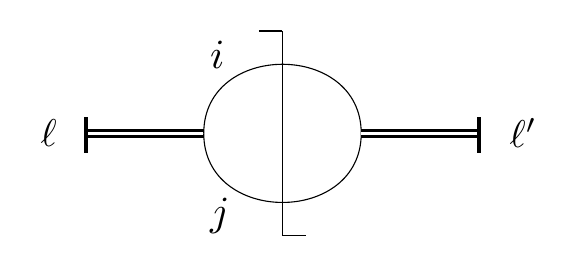
\begin{tikzpicture}
            \begin{feynman}
                % vertices
                \vertex (l) at (-2.5,0);
                \vertex (c1) at (-1,0);
                \vertex (c2) at (1,0);
                \vertex (r) at (2.5,0);
                \vertex (cut1) at (-0.3, 1.3);
                \vertex (cut2) at (0.0, 1.3);
                \vertex (cut3) at (0.0, -1.3);
                \vertex (cut4) at (+0.3, -1.3);
                % edge labels
                \vertex [left=5.5ptof l,scale=1.4] (tl) {$\ell$};
                \vertex [right=6.0pt of r,scale=1.4] (tr) {$\ell'$};
                \vertex [above right=18.0pt and -3.0pt of c1,scale=1.5] (ti) {$i$};
                \vertex [below right=18.0pt and -3.0pt of c1,scale=1.5] (tj) {$j$};
                % diagram
                \diagram* {
                    (l)
                    -- [double, line width=0.9pt, double distance=0.3ex, postaction={decorate, decoration={markings, mark=at position 0 with {\draw[line width=1.5pt] (0,-7pt) -- (0,6pt);}}}]
                    (c1)
                    ,
                    (c1) -- [half left] (c2) [dot]
                    ,
                    (c2) -- [half left] (c1) [dot]
                    ,
                    (c2)
                    -- [double, line width=0.9pt, double distance=0.3ex, postaction={decorate, decoration={markings, mark=at position 1 with {\draw[line width=1.5pt] (0,-7pt) -- (0,6pt);}}}]
                    (r)
                    ,
                    (cut1) -- (cut2) -- (cut3) -- (cut4)
                };
            \end{feynman}
        \end{tikzpicture}
        }}
        \hspace{-3pt}
        \ri]
        \,\,
        \Bigg/
        \,\,\text{\large$\dd \Phi_2(ij)$}
        \,,
    \end{align}
    where the parent particle \(\ell\) is denoted by a double line, the children \(i\) and \(j\) are both denoted by single lines (though they are potentially different), and \(\dd \Phi_2(ij)\) is the two-body Lorentz-invariant phase space associated with \(i\) and \(j\).
    \\
    For those unfamiliar with cut diagrams, an introductory reference is Chapter 24.1.2 of Matthew Schwartz' \underline{Quantum Field Theory and the Standard Model} \cite{Schwartz:2014sze}.
}


\remark{ignored-effects}{
    While we also averaged over final state spin information, we did not \emph{have} to do so, and we can also define analogous \textit{polarized} correlation matrices which depend also on the spin (or other quantum numbers) of the outgoing states \(i\) and \(j\).
    %
    On the other hand, there are several important effects that are thrown out by the stringent assumptions of \Prop{correlation-matrix-factorization} that cannot be so easily recovered.
    %
    Notably, the strict collinear limit we consider in this thesis erases additional kinematic and color correlations associated with \emph{spectators} of the splitting \cite{Catani:1996vz,Hoche:2014rga}.
}


\begin{exercise}
    \label{ex:massive-factorized-amplitudes}
    Prove that \Prop{correlation-matrix-factorization} still holds when particle masses are taken into account as long as \(m_i^2 + m_j^2 = m_\ell^2\) (with the notable application of \gls{qcd} with massive quarks when considering \(q \to g q\) splitting).
\end{exercise}


\remark{}{
    \Eq{amplitude-factorization} is an entry point into the theory of amplitudes.
    %
    In Yang-Mills theory, it is a special case of the Britto-Cachazo-Feng-Witten (BCFW) recursion relations \cite{Britto:2005fq,Arkani-Hamed:2008bsc} -- which provide a rigorous proof of (generalizations of) \Eq{amplitude-factorization} in an on-shell context.
    %
    The BCFW recursion relations can also be used to construct the \glslink{soft-limit}{soft} photon and \glslink{soft-limit}{soft} gluon theorems we discuss in \Sec{soft-gluons} \cite{Casali:2014xpa}.
    %
    The direct study of amplitudes provides powerful methods for the calculation of splitting structures in gauge theories and beyond \cite{Dixon:1996wi,Elvang:2015rqa}, but, as usual, is beyond the scope of this thesis.
}

The formulation of \Prop{correlation-matrix-factorization} may appear daunting, but when we restrict to a specific theory such as \gls{qcd}, dramatic simplifications tend to occur:

\begin{exercise}
    \label{ex:correlation-matrix-to-spin-matrix}
    Show that the correlation matrix \(\mathbb{C}_{(ij)}(\ell, \ell')\) is zero if \(\ell\) is a quark and \(\ell'\) is a gluon in \gls{qcd} for each possible collinear pair \((i,\,j)\).
    %
    More generally, use Lorentz invariance to argue that \(\mathbb{C}_{(ij)}(\ell, \ell')\) if \(\ell\) denotes a boson and \(\ell'\) denotes a fermion.

    \texttt{(Hint:)}
    %
    In the concrete example of \gls{qcd}, this can be quickly shown simply using the relevant three-point diagrams, without any computation.
\end{exercise}

The correlation matrices of \gls{qcd} cannot change particle type -- i.e. the particle corresponding to the label \(\ell\) is the same as the particle corresponding to the label \(\ell'\) -- nor color charge (this can be derived by direct computation -- see \Exercise{spin-correlation-exercise}).
%
We therefore define the simpler \vocab{spin correlation matrix} that will be useful for our explicit computations of splitting functions and splitting probabilities:

\begin{definitionbox}{Spin Correlation Matrices (e.g. of QCD)}{spin-correlation-matrix}
    Consider the situation where the correlation matrices \(\mathbb{C}_{(ij)}(\ell, \ell')\) for a given \(i\) and \(j\) are only non-zero for at most a single particle type, \(\text{type}(\ell) = \text{type}(\ell')\) (e.g. both are quarks or both are gluons), and are otherwise are diagonal in all labels \(L\) and \(L'\) (i.e. in the internal quantum numbers such as color, etc.) except for the spins of \(\ell\) and \(\ell'\).

    As I hope you showed in \Exercise{correlation-matrix-to-spin-matrix} above, this is true of \gls{qcd}.

    \vspace{7pt}
    \hrule
    \vspace{7pt}

    In this special case, we can simplify our analysis by using the \vocab{spin} \vocab{correlation} \vocab{matrix} \(\mathbb{S}\), defined by
    \begin{align}
        \mathbb{C}_{(ij)}(\ell, \ell')
        =:
        \begin{cases}
            0,&\ell \text{ and } \ell' \text{ have incorrect type}
            \\
            \delta_{L, L'}
            \mathbb{S}_{i j \leftarrow \ell}(s_\ell, s_\ell')
            &
            \text{otherwise}
            \,.
        \end{cases}
    \end{align}

    For example, the correlation matrices of \gls{qcd} when \(i = j = g\) are zero unless \(\ell\) and \(\ell'\) are both gluons.

    where again \(L\) and \(L'\) describe all possible quantum numbers of the particles \(\ell\) and \(\ell'\) except for their spin, and we abuse notation in the subscript of \(\mathbb{S}\) on the left hand side, writing \(\ell\) to denote the shared particle type of \(\ell\) and \(\ell'\).
\end{definitionbox}


The complicated general formulation of \Prop{correlation-matrix-factorization} can now be written more quickly in a relevant form for \gls{qcd}
\begin{lemma}{Spin Correlation Matrices Sew QCD Probabilities}{spin-correlation-factorization}
    When the spin correlation matrices of \Def{spin-correlation-matrix} are well-defined (as in \gls{qcd} at least at NLO), \Prop{correlation-matrix-factorization} implies that an \(N\)-particle amplitude in the limit that particles \(i\) and \(j\) are collinear can be written
    \begin{align}
        \overline{\sum} \abs{\mathcal{M}_N}^2
        =
        \frac{1}{2 k_i\cdot k_j}
        \overline{\sum}_{N-2}
        \sum_{L,\,s_\ell,\,s_\ell'}
        \mathcal{M}_{N-1}(\ell; L,\,s_\ell)
        \mathbb{S}_{ij \leftarrow \ell}(s_\ell, s_\ell')
        \mathcal{M}^*_{N-1}(\ell; L,\,s_\ell')
        \,,
    \end{align}
    where \(L\) denotes the internal quantum numbers of the particle \(\ell\) and \(s_\ell, s_\ell'\) denote its spin/helicity states.
\end{lemma}



\begin{answer}
       \begin{center}
        {\normalfont\Large\bfseries\sffamily The NLO QCD Spin Correlation Matrices are:}
    \end{center}


    Using the \(g \to g g\) amplitude from \Example{gtogg-amplitude},
    \begin{align}
        \label{eq:s_g_to_gg}
        \mathbb{S}_{g g \leftarrow g}(s_\ell, s_\ell')
        =
        4 \, C_A \, g_s^2
        \,
        \pmtrx{
            \frac{z}{1-z}+\frac{1-z}{z}+z(1-z)
            &
            z(1-z)\,e^{-2 i \phi}
            \\
            z(1-z)\,e^{2 i \phi}
            &
            \frac{z}{1-z}+\frac{1-z}{z}+z(1-z)
        }
        \,,
    \end{align}
    where \(C_A=N_C=3\) is the quadratic Casimir of the adjoint representation, and the upper row/first column corresponds to gluons of helicity \(+1\).
    %
    Using the \(q \to g q\) amplitude from \Example{qtoqg-amplitude},
    \begin{align}
        \label{eq:s_q_to_qg}
        \mathbb{S}_{g q \leftarrow q}(s, s')
        =
        2 g_s^2 C_F
        \,
        \frac{1 + \le(1-z\ri)^2}{z}
        \,
        \delta_{s, s'}
        \,,
    \end{align}
    where \(C_F = (N_C^2 - 1)/(2 N_C) = 4/3\) is the quadratic Casimir of the fundamental representation.
    %
    Finally, using the \(g \to q \overline{q}\) amplitude from \Exercise{gtoqq-amplitude},
    \begin{align}
        \label{eq:s_g_to_qq}
        \mathbb{S}_{q \overline{q} \leftarrow g}(\lambda, \lambda')
        =
        4 \, T_F \, g_s^2
        \,
        \pmtrx{
            z^2
            &
            -z(1-z)\, \cos(2\phi)
            \\
            -z(1-z)\,\cos(2\phi)
            &
            (1-z)^2
        }
        \,,
    \end{align}
    where \(T_F = 1/2\) is the Dynkin index of the fundamental representation.
\end{answer}

\begin{exercise}
    \label{ex:spin-correlation-exercise}
    Using the \gls{qcd} amplitudes of the cited examples and exercise, derive the spin correlation matrices of \gls{qcd} given above.

    \texttt{(Note:)}
    %
    To complete this exercise, I deigned to use a computer algebra system rather than my own weak hands, and the the polarization vectors and bispinors of \App{qcd-compendium} that I derived to simplify the polarization/spinor algebra of the collinear limit.
    %
    My rough code (which \textit{does not} involve importing more dedicated technology, like FeynCalc, etc.) is available on \href{https://github.com/samcaf/Thesis}{\texttt{the GitHub repository associated with this thesis at this https url}}.
    %
    Spinor helicity methods can also be a useful tool, if you know them.
\end{exercise}



\remark{angular-momentum-spin-correlation}{
    The off diagonal terms in the spin correlation matrices vanish upon azimuthal averaging.
    %
    Therefore, that is where we shall go next.
    %
    However, you may worry that they should not be there -- maybe that they ``break conservation of angular momentum'', so let us comment slightly more on their presence.
    %
    I will use ``child partons'' or ``children'' to refer to the children of a splitting -- i.e. in \(\mathbb{S}_{q\overline{q} \leftarrow g}\), the child partons are a quark and an anti-quark.
    %
    When we compute the spin correlation matrix, we project to a specific kinematic configuration of the child partons -- i.e. onto specific momentum eigenstates \(k_1\) and \(k_2\) -- determined by \(z,\theta,\) and \(\phi\).
    %
    By measuring in/projecting to a momentum eignbasis, we destroy any potential global angular momentum information associated with the wavefunction of the children due to the decay of the parent (it is encoded in the dependence of \(\mathcal{M}_{\ell \to i j}\) on the phase \(e^{i\phi}\)).
    %
    Therefore, the presence of the off-diagonal terms of the spin correlation matrix is an artifact of our projection in a momentum eigenbasis (rather than an angular momentum eigenbasis).
    %
    Indeed, that the off-diagonal terms vanish upon integration over \(\phi\) is a hint that angular momentum \textit{is} conserved when we integrate over the full \(k_1,k_2\) phase space, corresponding to a projection onto \textit{any} intermediate state of the pair \(i, j\).
    %
    When we perform a more inclusive projection of this type, the off-diagonal terms vanish and angular momentum appears once again to be ``conserved''.
}



%\begin{lemma}{Azimuthally Averaged Collinear Cross Sections}{collinear-cross-section}
%    In the \gls{collinear-limit}, \textbf{if} \(\mathbb{S}_{ij \leftarrow \ell}(\ell', \ell)\) is diagonal,
%    \begin{align}
%        \mathbb{S}_{ij \leftarrow \ell}(s_\ell', s_\ell)
%        :=
%        \frac{1}{2 k_i \cdot k_j}
%        \sum_{s_i,\, s_j}
%        \,
%        \mathcal{M}^*_{\ell \to i j}(s_\ell')
%        \,
%        \mathcal{M}_{\ell \to i j}(s_\ell)
%        \,
%        =:
%        \mathbb{S}_{ij \leftarrow \ell}
%        \,
%        \delta_{s_\ell'\, s_\ell}
%        \,,
%    \end{align}
%    where the diagonal part \(\mathbb{S}_{ij \leftarrow \ell}\) still depends on the momenta of \(\ell, i,\) and \(j\), \textbf{then} the cross section for \glslink{collinear-limit}{collinear} production of \(i\) and \(j\) factorizes:
%    \begin{align}
%        \dd \sigma_N
%        =
%        \dd \sigma_{N-1}
%        \,\,
%        \splitxsec{\ell}{ij}
%        \,\,
%        \frac{\dd\phi}{2\pi}
%        \,,
%    \end{align}
%    where
%    \begin{align}
%        \splitxsec{\ell}{ij}
%        :=
%        \frac{1}{4 \le(2 \pi\ri)^2}
%        \,\,
%        \mathbb{S}_{ij\leftarrow \ell}
%        \,\,
%        \dd z
%        \,
%        \frac{\dd s}{s}
%        \,,
%    \end{align}
%    and \(s = (k_i + k_j)^2 = 2 k_i \cdot k_j\).
%    %
%    \(\splitxsec{\ell}{ij}\) is not a differential cross section itself;
%    %
%    its name is meant to indicate that it appears in cross sections in the \gls{collinear-limit} for processes involving the splitting \(\ell \to i,\, j\).
%\end{lemma}

%\remark{}{
%    Though the \emph{assumptions} of \Lem{collinear-cross-section} are generally false, as can be seen in e.g. Examples~\ref{ex:gtogg-split} and \ref{ex:qtoqg-split}, the purpose of this lemma is to illuminate the structural features of the factorization we are about to see.
%}


%Unfortunately, as we have seen, the quantities \(\mathbb{S}_{ij \leftarrow \ell}(s_{\ell}', s_\ell)\) are \textit{not} diagonal.
%%
%To pursue the splitting functions of \gls{qcd}, we will perform one more trick:
%%
%we will integrate over the azimuthal angle associated with the outgoing \(k_i\) and \(k_j\) to eliminate non-diagonal terms.
%%
%Defining \(\le\langle A \ri\rangle_\phi = \int_0^{2\pi} A / 2\pi\), the azimuthally averaged amplitudes of \gls{qcd},
%\begin{align}
%    \le\langle \splitxsec{\ell}{ij}\ri \rangle_\phi
%    :=
%    \int_0^{2\pi} \frac{\dd \phi}{2\pi}
%    \,\,
%    \splitxsec{\ell}{ij}
%    \,,
%\end{align}
%\textit{will} be diagonal.
%%
%The derivation of \Lem{collinear-cross-section} can proceed as before, this time with an additional azimuthal integral, and obtain its the azimuthally-averaged analogue:


\begin{lemma}{Azimuthal Averages of Collinear Cross Sections}{averaged-collinear-cross-section}
    In the \gls{collinear-limit}, \textbf{if} the azimuthal average of the spin correlation matrix,
    \begin{align}
        \le\langle\mathbb{S}_{ij \leftarrow \ell}(\ell', \ell)\ri\rangle_\phi
        :=
        \int_0^{2\pi}
        \frac{\dd \phi}{2\pi}
        \mathbb{S}_{ij \leftarrow \ell}(\ell', \ell)
    \end{align}
    is diagonal%
    \footnote{
        Certainly true of \gls{qcd} at NLO, and I \textit{think} guaranteed more generally by conservation of angular momentum, see Remark~\ref{rem:angular-momentum-spin-correlation}.
    }
    %
    and more specifically proportional to the identity%
    \footnote{
        Not true of \gls{qcd} -- see \(\mathbb{S}_{q\overline{q}\leftarrow g}\) in \Eq{s_g_to_qq}.
    }
    \begin{align}
        \le\langle\mathbb{S}_{ij \leftarrow \ell}(s_\ell', s_\ell)\ri\rangle_\phi
        =
        \le\langle\mathbb{S}_{ij \leftarrow \ell}\ri\rangle_\phi
        \,
        \delta_{s_\ell'\, s_\ell}
        \,,
    \end{align}
    \textbf{then} the azimuthally-averaged cross section for \glslink{collinear-limit}{collinear} production of \(i\) and \(j\) factorizes:
    \begin{align}
        \le\langle
        \dd \sigma_N
        \ri\rangle_\phi
        =
        \dd \sigma_{N-1}
        \,\,
        \splitxsec{\ell}{ij}
        \,,
    \end{align}
    where
    \begin{align}
        \splitxsec{\ell}{ij}
        :=
        \frac{\dd z \, \dd s}{16 \pi^2 s}
        \le\langle\mathbb{S}_{ij\leftarrow \ell}\ri\rangle
        \,.
    \end{align}
\end{lemma}

\begin{proof}
    This lemma is a quick fusion of the previous results of this section and the \glslink{collinear-limit}{collinear} phase space factorization discussed in \Lem{collinear-phase-space-azimuthal}.
    %
    First, we recall that the differential cross section takes the form
    \begin{align}
        \dd \sigma_N
        =
        F_\text{init.}
        \overline{\sum}\abs{\mathcal{M}_N}^2
        \dd \Phi_N
    \end{align}
    where \(F_\text{init.} = (u_\alpha E_{p_1} E_{p_2})^{-1}\) is a factor that depends only on the initial state, and is thus shared by \(\dd\sigma_{N}\) and \(\dd\sigma_{N-1}\), which differ only in their final states.%
    \footnote{
        In case our notation is getting too cumbersome, I recall here that the \(N-1\)-particle process has the collinear \(i\) and \(j\) replaced by an off-shell \(\ell^*\).
    }

    Using \(\dd\Phi_N = \dd\Phi_{N-1} \dd\Phi_{+1}\) with \(\dd\Phi_{+1} = \dd z \dd s \dd \phi / 32 \pi^3\) (in four dimensions, though see \Exercise{d-dimensional-splitting}), and the assumption that the azimuthal average of the spin correlation matrix is proportional to the identity, \(\le\langle \mathbb{S}_{ij\leftarrow \ell}(s',s) \ri\rangle := \le\langle\mathbb{S}_{ij\leftarrow \ell}\ri\rangle \delta_{s' s}\), we have
    \begin{align}
        \le\langle \dd \sigma_N\ri\rangle
        =
        \frac{1}{s}
        \le\langle\mathbb{S}_{ij\leftarrow \ell}\ri\rangle
        \frac{\dd\Phi_{+1}}{\dd\phi / 2\pi}
        \,\,\,
        F_{\text{init}}
        \,
        \overline{\sum}_{N-2}
        \sum_{L, s_\ell}
        \abs{\mathcal{M}_{N-1}(\ell; L, s_\ell)}^2
        \,
        \dd\Phi_{N-1}
        =
        \frac{\dd z \, \dd s}{16 \pi^2 s}
        \le\langle\mathbb{S}_{ij\leftarrow \ell}\ri\rangle
        \,\,
        \dd\sigma_{N-1}
        \,,
    \end{align}
    where we have performed the azimuthal integral \(\dd\phi/2\pi\) within \(\dd\Phi_{+1}\) to obtain the azimuthal average.
    %
    Here, \(\dd\sigma_{N-1}\) is the differential cross section to produce a \textit{nearly} on-shell \(\ell\) -- eventually, in \Chap{jets}, we will need to show that \(\ell\) can be treated on-shell to continue recursively.
    %
    For now, however, the lemma is proved.
\end{proof}


\begin{exercise}
    \label{ex:d-dimensional-splitting}
    Repeat the proof of \Lem{averaged-collinear-cross-section} in \(d = 4 - 2\epsilon\) dimensions.
    %
    I find
    \begin{align}
        \splitxsec{\ell}{ij}
        =
        \frac{\le(4\pi\ri)^\epsilon z^{-\epsilon}(1-z)^{-\epsilon} s^{-\epsilon}}{\Gamma(1-\epsilon)}
        \frac{\dd z \, \dd s}{16 \pi^2 s}
        \le\langle\mathbb{S}_{ij\leftarrow \ell}\ri\rangle
        \,.
    \end{align}

    When using this formula in practice -- as we do in the calculation of the fixed-order behavior of the \glslink{eec}{energy-energy correlator} in \Chap{ewocs} -- one will nearly always take \(g_s\) to be a dimensionless coupling constant.
    %
    I point this out because any factors of \(g_s\) in \(\mathbb{S}_{ij \leftarrow \ell}\) must then be replaced by \(\mu^\epsilon g_s\) (the coefficient of the term \(\overline{\psi} \slashed{A} \psi\) in a \(d\)-dimensional Lagrangian must have mass dimension \(\epsilon\)).%
    \footnote{
        In the computation of \Chap{ewocs}, we instead use a more complicated multiplicative factor for \(g_s\), \(g_s \to (\mu \cdots)^\epsilon g_s\), to simplify computations, but the philosophy is the same.
    }
\end{exercise}




In practice we often \textit{pretend} that \(
        \le\langle\mathbb{S}_{ij \leftarrow \ell}(\ell', \ell)\ri\rangle_\phi
\) in order to proceed -- in particular for the case \(g \to q \overline{q}\).
%
In \gls{qcd}, where the terms which violate this assumption are finite in the limit \(z \to 0\) or \(z \to 1\), this is justified by the use of the \textit{\gls{soft-limit}}, which will become an essential piece of our analysis in this thesis.
%
In particular, there are terms in the \(\mathbb{S}_{ij \leftarrow \ell}\) which become \textit{infinite} in the soft limit, and therefore dominate the defining characteristics of partonic radiation.
%
As long as the terms which violate the assumptions of \Lem{averaged-collinear-cross-section} are not singular terms, they are sub-leading in the soft limit, and we can manipulate them to make our lives easier without dramatically affecting the accuracy of our results.


\textbf{In the soft limit of QCD, we are able to replace \(\mathbb{S}_{ij \leftarrow \ell}(s, s')\) by the average/identity component \(\delta_{s s'} \Tr \mathbb{S}_{ij \leftarrow \ell}/2\) to apply \Lem{averaged-collinear-cross-section} to the factorization of differential cross sections.}
%
Strictly speaking, this replacement loses some information about spin correlations, but the corrections to this approximation are unimportant in the \gls{soft-limit}.


Overcoming this subtlety, \Lem{averaged-collinear-cross-section} then motivates the following definition for \vocab{splitting functions}:
\begin{definitionbox}{(Unpolarized) Splitting Functions}{splitting-function}
    A \vocab{\gls{splittingfn}} describes the probability distribution (approximately, up to sub-leading terms in the soft limit) for an intermediate parent parton \(\ell\) to split into collinear children \(i\) and \(j\):
    \begin{align}
        \le\langle
        \splitxsec{\ell}{ij}
        \ri\rangle_\phi
        \Big|_{E_i / E_{\ell} = z_i}
        \approx
        \frac{\alpha_s}{2\pi}
        P_{ij\leftarrow \ell}(z_i)
        \frac{\dd z_i \, \dd s}{s}
        \,,
    \end{align}
    with
    \begin{align}
        P_{ij \leftarrow \ell}(z_i)
        :=
        \frac{
            \frac{1}{2}
            \le\langle
            \Tr \mathbb{S}_{ij\leftarrow \ell}
            \ri\rangle_\phi
            \Big|_{E_i / E_{\ell} = z_i}
        }{2 g_s^2}
        \,.
    \end{align}


    \vspace{10pt}
    \hrule
    \vspace{10pt}

    More precisely, the \(P_{ij \leftarrow \ell}\) are called \vocab{exclusive splitting functions}.
    %
    An \vocab{inclusive splitting function} is a splitting function which is \textit{inclusive} over (meaning ``sums over'') the possible state \(j\), and is denoted by a lowercase \(p\):
    \begin{align}
        p_{i\leftarrow \ell}(z_i)
        =
        \sum_j P_{i j \leftarrow \ell}(z_i)
        \,.
    \end{align}
\end{definitionbox}


 \remark{polarized-splitting-functions}{
     There are also \textit{polarized} \glspl{splittingfn}, which retain more detailed information about the polarizations of the children \(i,\,j\) of a splitting.
    %
    They can be computed via analogous procedures using the polarized correlation matrices discussed briefly in Remark~\ref{rem:ignored-effects}.
    %
    Some discussion of polarized splitting functions is given in the original paper of Altarelli and Parisi \cite{Altarelli:1977zs}.
}


\remark{}{
    Splitting functions give us one of the first quantitative hints of jets we have presented in this thesis.
    %
    The recursive use of splitting functions and splitting probabilities will be used to construct the partonic cascade model for jet formation in \Sec{parton-shower}.
    %
    Before we are ready to take on that challenge, however, we will need to develop some additional technology involving the physics of \emph{soft gluons}, discussed in \Sec{soft-gluons}.
    %
    It will also be useful to perform some fixed-order computations related to the substructure of jets in \Sec{fixed-order-substructure}, which will both give us some practice with calculations and re-emphasize the problem of infra-red divergences in physical predictions that \Chap{jets} will solve.
}


We will use these functions to describe the probability that collinear partons are produced in a high-energy scattering event, which, as we show in \Chap{jets}, leads to the formation of jets in collider experiments.
%
Their singular structure at \(z = 0\) (and, for the gluon splitting function, \(z = 1\)) is a hurdle we will match soon.
%
For now, however, let us consolidate some of our results for \gls{qcd}:

\begin{example}
    \label{ex:qcd-splitting-functions}

    Using the tabulated values of the NLO spin correlation matrices in \Eqss{s_g_to_gg}{s_q_to_qg}{s_g_to_qq}, the splitting functions of \gls{qcd} are (away from zero -- see the discussion below)
    \begin{align}
        P_{gg \leftarrow g}(z)
        &=
        2C_A \le(\frac{1-z}{z} + \frac{z}{1-z} + z(1-z)\ri)
        \\
        P_{gq \leftarrow q}(z)
        &=
        C_F \frac{1 + (1-z)^2}{z}
        \\
        P_{q\overline{q} \leftarrow g}(z)
        &=
        T_F \le(z^2 + \le(1-z\ri)^2\ri)
        \,.
    \end{align}
    For ease of notation, we also denote \(P_{q \overline{q} \leftarrow g}(z)\) by \(P_{qq\leftarrow g}(z)\).
\end{example}


\begin{exercise}
    \label{ex:qcd-inclusive-splitting}
    Using the exclusive splitting functions of \Example{qcd-splitting-functions}, compute the \emph{inclusive} splitting functions of \gls{qcd}.
\end{exercise}



\epigraph{I lied.}{\href{https://www.youtube.com/watch?v=_wk-jT9rn-8}{Arnold Schwarzenegger, \textit{Commando}}}

We will eventually pursue a probabilistic interpretation of the splitting functions \(P_{ij \leftarrow \ell}(z)\), as the probability that a parton of type \(\ell\) splits into partons of type \(i\) and \(j\) with momentum fraction \(z = z_i\).
%
However, the splitting functions we derived above, with the exception of \(P_{q\overline{q} \leftarrow g}\), are clearly non-integrable.
%
This is undoubtedly a problem we must overcome to think of splitting functions as related to probabilities.

Traditionally, one states that virtual contributions must come in to save the day and regularize the splitting functions because of the KLN theorem (\Thm{kln}).
%
But I have never seen a proof or an argument that has fully satisfied me, and I have been hurt too many times (see \Sec{irc-safety} -- especially Lore~\ref{lore:irc-safety-lore} and Remark~\ref{rem:multiple-soft-emissions-break-invariance} -- and Remark~\ref{rem:ward-warning}).
%
Therefore I warn that

\remark{i-dont-know-splitting}{
    \textbf{Within the framework I have derived above, I know of no way to regularize our splitting functions or derive their probabilistic interpretation.}
}

Nonetheless, forgive me as I continue with the standard lore.
%
It states that we must add in terms proportional to delta functions, said to be associated with diagrams in which \textit{no} emission occurs, in order to yield a probabilistic interpretation of the splitting functions.

We therefore use \textit{physical} reasoning, associated with the interpretation of the splitting functions as associated to normalized distributions.
%
In particular, we make the common choice to use \glslink{plus-fn}{\vocab{plus-function regularization}}:

\begin{definitionbox}{Plus-Function Regularization}{plus-function-regularization-simple}
    A \vocab{plus-distribution} (or ``\vocab{plus-function}'') is a modified, integrable version of a ``parent function'' which is often so singular that it cannot be integrated on its own.

    \vspace{7pt}
    \hrule
    \vspace{7pt}

    For a function \(f(z)\) with support in \(z \in (0,1)\), as in the cases of physical interest in this thesis, a plus-function can be defined either in terms of its behavior when integrated against test functions \(g(z)\).
    %
    In particular, if \(f(z)\) is singular%
    \footnote{With a singularity no worse than a simple pole, though see Remark~\ref{rem:more-singular-plus-functions} in \App{plus-functions}.}
    %
    at zero, then we write
    \begin{align}
        \label{eq:plus-fn-simple-main}
        \int \dd z'
        \,
        [f(z')]_+
        \,
        g(z')
        :=
        \int \dd z'
        \,
        f(z')
        \,
        \le(g(z') - g(0)\ri)
        \,.
    \end{align}
    %
    We call \([f(z)]_+\) the \vocab{plus-function regularized} form of \(f(z)\).
    %
    Formally, \Eq{plus-fn-simple-main} is sometimes written in the schematic form
    \begin{align}
        \label{eq:plus-fn-simple-delta}
        [f(z)]_+
        =
        f(z)
        -
        \,
        \delta(z)
        \,\,
        \int \dd z'
        \,
        f(z')
        \,,
    \end{align}
    where it is understood that \([f(z)]_+\) must be integrated against a sufficiently well-behaved test function.
    %
    Similar definitions hold if the function is singular at \(z=1\), in which case e.g. the factor of \(\delta(z)\) in \Eq{plus-fn-simple-delta} is replaced by \(\delta(1-z)\).

    For more detail, general definitions, and several examples, see \App{plus-functions}.
\end{definitionbox}

Importantly, a plus-regularized function integrates to zero:
\begin{align}
    \int\dd z'
    \,\,
    [f(z')]_+
    =
    0
    \,.
\end{align}

\begin{exercise}
    \label{ex:plus-fn-replacement}
    Argue that, for a function \(f(z)\) singular that is singular at \(z = 0\) and a function \(h(z)\) that is sufficiently regular, we can write
    \begin{align}
        h(z) [f(z)]_+
        =
        [h(z)\,f(z)]_+
        \,\,
        +
        \,
        \delta(z)
        \,
        \int \dd z'
        \,\,
        [f(z')]_+
        \,
        h(z')
        \,.
    \end{align}
    A complete argument should in part involve defining notation more precisely.

    We will also use the common notation
    \begin{align}
        \frac{a(z)}{(z)_+}
        \,
        :=
        \,
        a(z)\le[\frac{1}{z}\ri]_+
        \,.
    \end{align}
\end{exercise}




\remark{process-dependent-plus}{
    The emergence of plus-function-regularized splitting functions can certainly be seen directly in process-dependent calculations.
    %
    For example, in dimensional regularization in calculations of the cross section for \(e^+ e^-\) to hadrons, the emergence of infrared divergent virtual diagrams lead to terms (roughly) proportional to \(2 a_s C_R \,\, \delta(z)\,/\,\epsilon\), while the phase space distribution associated with a splitting is proportional to \(2 a_s C_R z^{-1-\epsilon} = -2 a_s C_R\,\,  \delta(z) / \epsilon\,\, + \, \, 2 a_s C_R \,\, \le[1/z\ri]_+\) (see \Prob{plus-identity}, borrowed from Schwartz' \underline{Quantum Field Theory and the Standard Model} \cite{Schwartz:2014sze}).
    %
    It is a simple and process-\emph{independent} proof in the context of the collinear limit of partonic factorization -- i.e. our discussion so far in \Sec{universal-features} -- that I am missing.
    %
    If you know one which is satisfying and includes a complete calculation, please reach out.
    %
    I note that Collins' \underline{Foundations of Perturbative QCD} \cite{Collins:2011zzd} provides methods for deriving splitting functions and more (such as the probability of finding quarks inside other quarks), through a more rigorous philosophy based on the operator product expansion, and requires the use of composite operator renormalization.
    %
    For more historical presentations of the use of the OPE and renormalization in deriving splitting behavior, tied tightly to structure functions, see also \Reffs{Gross:1973zrg,Georgi:1974wnj}
}

To begin, we consider the splitting of a parton of flavor \(\ell\).
%
Standard lore asks us to recall the behavior of the full splitting distribution,
\begin{align}
    \dsigmatilde_{ij \leftarrow \ell}
    =
    \frac{\alpha_s}{2\pi}
    P_{ij \leftarrow \ell}(z_i) \frac{\dd z_i \dd s}{s}
    \,,
\end{align}
and, in the probabilistic interpretation, the total NLO probability distribution for the splitting to occur with momentum fraction \(z = E_i/E_\ell\) is obtained by integrating over the virtuality \(s\):
\begin{align}
    \rho_{ij \leftarrow \ell}(z)
    =
    \frac{\alpha_s}{2\pi}
    P_{ij \leftarrow \ell}(z_i)
    \,\,
    L
    \,,
\end{align}
where \(L := \int \dd s / s\) (\(L\) stands for ``logarithmically divergent'');
%
the upper bound on the integration over \(s\) is determined by the process in question, but it is safe to say that the integral is UV-finite:
%
\(s < E_\text{c.m.}^2\).
%
The lower bound in massless \gls{qcd} is zero, however, and the integral is IR-divergent.


Nonetheless, less us proceed with the \emph{formal manipulations} that will lead us to standard foundational results.
%
We now write the probability distribution to find a parton of flavor \(i\) \textit{inside} our original quark, of relative momentum fraction \(z\), as
\begin{align}
    \rho_{i \leftarrow \ell}(z)
    =
    \delta_{i\ell}
    \,
    \delta(1-z) + \sum_j \rho_{ij \leftarrow \ell}(z)
    \,
    =
    \,
    \delta(1-z)
    \,
    +
    \,
    \frac{\alpha_s}{2\pi}
    p_{j\leftarrow \ell}(z)
    \,\,
    L
    \,,
\end{align}
where we have used the definition of the \textit{inclusive} splitting function \(p\), and we have integrated the full splitting distribution.%
\footnote{
    Beyond NLO, we must include additional splitting functions with a more complicated structure.
    %
    At NNLO, for example, there are \(1 \to 3\) splitting functions describing the probability of a single parton converting into three partons \cite{Campbell:1997hg,Catani:1999ss} (see also \Reff{Larkoski:2024uoc} and references therein).
    %
    Nonetheless, the structure of \(\rho_{i\leftarrow \ell}\) can easily be extended, e.g. by summing over \emph{two} final-state partonic flavors in the \(1\to 3\) splitting functions to isolate the index \(i\) and, more generally, \(N-1\) final-state flavors for \(1\to N\) splitting functions.
}



Following the socio-physical arguments above, we ``include the effects of virtual contributions'' by writing, schematically
\begin{align}
    \label{eq:start-regularizing}
    p_{j\leftarrow \ell}(z)
    =
    H^{(0)}_{j\ell} \delta(z)
    +
    H^{(1)}_{j\ell} \delta(1-z)
    +
    [p_{j\leftarrow \ell}(0<z<1)]_+
    \,,
\end{align}
where \(H\) (for ``ad Hoc'') indicates terms that we have added in by hand for the validity of the NLO probabilistic interpretation, and the argument of the final term indicates that it corresponds to the non-regularized splitting functions we derived above.


The physical intuition used to constrain the coefficients \(H\) in the regularized form of the splitting functions presented in \Eq{start-regularizing} is quantified through \vocab{\glspl{sum-rule}}:
%
rules dictating the values of integrals of distributions obtained through \gls{qft} methods -- in our case, integrals involving the \gls{qcd} splitting functions.
%
The sum rules we use to constraint the regularized form of splitting functions are framed physically in terms of \textit{conservation laws}.


We begin by using \emph{conservation of baryon number}%
\footnote{
    In the full \gls{sm}, the classical global symmetry that would preserve baryon number is anomalous, and therefore unavailable to produce a conservation law at the quantum level.
    %
    However, in massless \gls{qcd}, there is no anomaly.
}
%
to constrain the quark-to-quark inclusive splitting function.
%
Our analysis holds at NLO.
%
At N\(^2\)LO, the quark can split into a quark and a gluon, and the gluon can split into a quark and an anti-quark.
%
A baryon-number-conservation sum rule at N\(^2\)LO then must also involve the associated splitting probability for anti-quark production, \(p_{\overline{q} \leftarrow q}\).

\begin{example}
    \label{ex:p_qq-baryon-number}

    For a fixed quark flavor, the \vocab{baryon-number-conservation \gls{sum-rule}} states that the number of quarks we find inside a quark (ignoring NNLO production of anti-quarks) should be one:
    \begin{align}
        \int_0^1 \dd z'
        \rho_{q \leftarrow q}(z')
        = 1
        \,,
    \end{align}
    implying \(\int_0^1 \dd z' p_{q\leftarrow q}(z') \,\, =\,\, \int_0^1 \dd z' P_{gq \leftarrow q}(z') = 0\), and therefore \(H^{(0)}_{qq} + H^{(1)}_{qq}\).
    %
    This gives us one equation.
    %
    The next is another sociological one:
    %
    lore tells us that if there is no singularity in the splitting function, there should be no regularization.
    %
    Since the \(p_{q\leftarrow q}(z)\) has no singularities at \(z = 0\), we therefore take \(H^{(0)}_{qq} = 0\).
    %
    Therefore, the sociologically-plus-regulated form of \(p_{q\leftarrow q}(z)\) is
    \begin{align}
        p_{q \leftarrow q}(z)
        =
        P_{qg \leftarrow q}(z)
        =
        C_F \le[\frac{1 + z^2}{(1-z)}\ri]_+
        \,,
    \end{align}
    and, accordingly,
    \begin{align}
        p_{g \leftarrow q}(z)
        =
        P_{gq \leftarrow q}(z)
        =
        C_F \le[\frac{1 + (1-z)^2}{z}\ri]_+
        \,.
    \end{align}
\end{example}

\begin{exercise}
    Using \Exercise{plus-fn-replacement}, show that
    \begin{align}
        p_{g \leftarrow q}(z)
        \,
        =
        \,
        C_F
        \,\,
        \le(1+(1-z)^2\ri)
        \le[\frac{1}{z}\ri]_+
        +
        A \delta(z)
        \,.
    \end{align}
    What is the numerical value of the coefficient \(A\)?
\end{exercise}


Again applying the lore that splitting functions only receive virtual corrections when they are infra-red divergent, we also take \(p_{q \leftarrow g}(z) = T_F \le(z^2 + (1-z)^2\ri)\), for a single quark flavor \(q\), even after regularization.
%
When \(N_f\) quark flavors are involved, and we use \(p_{g \leftarrow g}(z)\) to denote the inclusive splitting function for the production of \emph{any} quark \emph{or} anti-quark regardless of flavor, we will often run into the combination
\begin{align}
    \sum_{f=1}^{N_f}
    \sum_{i \in \{q_f, \overline{q}_f\}}
    p_{i \leftarrow g}(z)
    =
    2 N_f T_F \, \le(z^2 + (1-z)^2\ri)
    \,.
\end{align}


For gluons, our final ingredient, we can invoke symmetry under \(z \leftrightarrow 1-z\) to write \(H^{(0)}_{gg} = H^{(1)}_{gg}\).%
\footnote{
    This symmetric representation for \(p_{gg}(z)\) is non-standard, and it is common to only regularize the \(z=1\) singularity of \(p_{g\leftarrow g}(z)\).
    %
    However, we stand by the symmetry of the gluon splitting function in the physically-motivated discussion of this chapter.
    %
    We should note that, according to \Reff{Altarelli:1977zs}, using a symmetric representation of the regularized \(p_{gg}\) does not directly translate into familiar DGLAP renormalization evolution for \emph{all} structure functions (see discussion near their Eq. (37)).
    %
    However, differences due to our symmetric representation here arise (\emph{only}) in the \(m\leq1\) Mellin moments (see e.g. \App{mellin}) of \(p_{gg}(z)\).
    %
    We do not use \(m=1\) Mellin moments directly in this thesis, and the symmetric representation yields correct results for all higher-order Mellin moments.
    %
    Furthermore, since the Mellin transform of the symmetric and standard representations, the \(\hat{p}_{gg}(m)\), are analytic and agree for \(\Re m > 1\), the identity theorem suggests that they must have the same analytic continuation.
}
%
we have no number conservation sum rule.
%
But we have \emph{the conservation of momentum}.

\begin{example}
    The \vocab{momentum conservation \gls{sum-rule}} takes the form
    \begin{align}
        \int_0^1\,\dd z'\,\, z'\,\rho_{i\leftarrow\ell}(z') = 1
        \,,
    \end{align}
    and therefore constrains the \textit{gluon splitting functions} via
\begin{align}
    \int_0^1 \dd z'
    \,\,
    z'
    \,\,
    \sum_i
    p_{i \leftarrow g}(z')
    =
    \int_0^1 \dd z'
    \,\,
    z'
    \,\,
    \le(
        2 N_f p_{q \leftarrow g}(z')
        +
        p_{g\leftarrow g}(z')
    \ri)
    = 0
    \,.
\end{align}
%
Our known expression for \(p_{q\leftarrow g}\) gives
\begin{align}
    2 N_f \,\int_0^1 \dd z'\,\, z'\,\, p_{q \leftarrow g}(z')
    \,
    =
    \,
    \frac{2}{3}\,N_f T_F
    \,,
\end{align}
so that \(\int \dd z'\,\, z'\,p_{g\leftarrow g}(z') = -2/3 N_f T_f \).
%
Now we explicitly regularize by writing
\begin{align}
    p_{gg}(z')
    :=
    2 C_A \le(
        \frac{1-z}{(z)_+} + \frac{z}{(1-z)_+} + z(1-z)
    \ri)
    \,\,
    +
    \,\,
    H_{gg}\delta(z) + H_{gg} \delta(1-z)
    \,,
\end{align}
which gives
\begin{align}
    \int \dd z'\,\, z'\,p_{g\leftarrow g}(z')
    =
    2 C_A \le(\frac{1}{2} - \frac{3}{2} + \frac{1}{12}\ri)
    +
    H_{gg}
    =
    -\frac{11}{6}\,C_A + H_{gg}
    \,.
\end{align}
To satisfy the sum rule, we must set
\begin{align}
    H_{gg} = \frac{11}{6} C_A - \frac{2}{3} N_f T_F
    \,.
\end{align}

We also note the miraculous appearance of half of the \gls{qcd} beta function coefficient,
\begin{align}
    \beta_0 = \frac{11}{3} C_A - \frac{4}{3}N_f T_F
    \,.
\end{align}
\end{example}

\begin{exercise}
    Show that the behavior of the regularized quark splitting functions ``derived'' above is consistent with momentum conservation.
\end{exercise}

\begin{exercise}
    Write a general form for the sum rule on splitting functions associated with a conserved quantum number \(\chi\).
\end{exercise}



With a combination of physical intuition and sociological evidence we have found, now including regularization:
\begin{answer}
    \begin{center}
        {\normalfont\Large\bfseries\sffamily The Regularized NLO QCD Splitting Functions are:}
    \end{center}

    \begin{subequations}
    \begin{align}
        \label{eq:p_gtogg}
        P_{gg \leftarrow gg}(z)
        &=
        2C_A \le(
            \frac{1-z}{(z)_+}
            +
            \frac{z}{(1-z)_+}
            +
            z(1-z)
        \ri)
        \,\,
        +
        \,\,
        \frac{\beta_0}{2}
        \,
        \le(\delta(z) + \delta(1-z)\ri)
        \,,
        \\
        \label{eq:p_qtogq}
        P_{gq \leftarrow q}(z)
        &=
        C_F \le[\frac{1+\le(1-z\ri)^2}{z}\ri]_+
        \,,
        \\
        \label{eq:p_gtoqq}
        P_{q\bar{q} \leftarrow g}(z)
        &=
        T_F \left(z^2 + (1-z)^2\right)
        \,.
    \end{align}
    \end{subequations}
\end{answer}


We are done with one of the most important steps in our preparation for understanding jets.
%
We now understand the distributions by which energy is divided when a nearly-on-shell particle ``splits'' into two.
%
Next, we will study the \textit{angular} behavior of radiation patterns.
%
By combining our understanding of the energy and angular distributions of \gls{qcd} radiation, we will describe the flow of energy in the partonic cascade in \Chap{jets}.
%
We will be left with a powerful and relatively simple framework through which we calculate and quantify the inner lives of quarks and gluons.
%
Therefore, we take our next step.
%
To angles!


% ---------------------------------------
\subsection{Soft Gluons are Angular-Ordered}
% ---------------------------------------
\label{sec:soft-gluons}

\epigraph{The art of doing mathematics consists in finding that special case which contains all the germs of generality.}{David Hilbert}

The factorization formulae of this section all hold in the \textit{eikonal limit}, which for our purposes describes the physics of particles which are very low-energy or very \glslink{collinear-limit}{collinear}:

\begin{definitionbox}{Eikonal Limit}{eikonal-limit}
    In \gls{qft}, the \vocab{eikonal limit} refers to a limit in which the four-momenta of two particles become nearly \glslink{collinear-limit}{collinear}.
    %
    More precisely, the \vocab{eikonal limit for particles \(i\) and \(j\)} is associated with the region of phase space in which the pair of particles \(i\) and \(j\) are far more \glslink{collinear-limit}{collinear} than any other pair of particles in a scattering event:
    \begin{align}
        \label{eq:eikonal-limit}
        p_i \cdot p_j \ll p_\ell \cdot p_m\qquad \forall \,\, \ell\neq m
        \,.
    \end{align}
\end{definitionbox}


\remark{}{
    The eikonal limit for massless particles \(i\) and \(j\) implies that either \(i\) and \(j\) are very \glslink{collinear-limit}{collinear} or that at least one is very low energy.
    %
    In particular, setting \(i = \ell\) in \Eq{eikonal-limit} and using massless particles, for which \(
        p_i \cdot p_j
        =
        E_i E_j \le(1 - \hat{n}_i \cdot \hat{n}_j\ri)
    \),
    %
    we have
    \begin{align}
        E_j \le(1 - \hat{n}_i \cdot \hat{n}_j\ri)
        \ll
        E_k \le(1 - \hat{n}_i \cdot \hat{n}_k\ri)
        \,,
    \end{align}
    for all \(k\).
    %
    If we write \(1-\hat{n}_\ell \cdot \hat{n}_m \approx \theta^2_{\ell m}/2\), we can conclude that for all \(k\),
    \begin{align}
        E_j \theta^2_{ij}
        \ll
        E_k \theta^2_{ik}
        \,,
    \end{align}
    and similarly when \(i\) and \(j\) are flipped.
    %
    If \(E_j\) and \(E_k\) are of similar magnitude, \(E_j \sim E_k\), then \(\theta^2_{ij} \ll \theta^2_{ik}\);
    %
    otherwise, if \(\theta^2_{ij} \sim \theta^2_{ik}\), then \(E_j \ll E_k\).
    %
    Therefore, either \(\theta^2_{ij} \ll \theta^2_{ik}, \theta^2_{jk}\) or \(E_i, E_j \ll E_k\), for all \(k\).
}



Closely related is the \textit{\glslink{soft-limit}{soft} limit} involving only a single particle:
\begin{definitionbox}{Soft Limit}{soft-limit}
    The \vocab{\gls{soft-limit}} for a particle with momentum \(q\) is the limit in which the particle is eikonal with respect to any \textit{other} particle/pair of particles in the scattering event:
    \begin{align}
        q \cdot p_i \ll p_j \cdot p_k
        \qquad
        \forall\,i,j,k,
        \,\,
        j\neq k
        \,,
    \end{align}
    where the \(p_j\) and \(p_k\) do not include \(q\).
    %
    In what follows in this section, we also say that the particle with momentum \(q\) is \vocab{soft}.
\end{definitionbox}


The eikonal limit was originally used as a tool in geometric optics (hence the name, from the Greek \(\varepsilon \acute{\iota}\kappa \acute{\omega}\nu\), meaning `image'' and the root of the more common English word ``icon'').
%
Once light was discovered to be a wave, the eikonal limit was taken from optics and applied to the more general mechanics of waves.
%
Today, it is used in the description of waves in electromagnetism, non-relativistic quantum mechanics, and our current context:
%
particle physics and quantum field theory.

In \gls{qft} the eikonal limit describes universal features of the radiation accompanying charged matter;
%
roughly, it captures features of the cloud of photons corresponding to the electric field surrounding an electron, and the cloud of gluons accompanying quarks.
%
Due to the universality of eikonal radiation, the amplitudes describing scattering in gauge theories -- including electrodynamics, \gls{qcd}, the \gls{sm}, and even gravity -- take a remarkably simple form.

An early an extremely powerful result demonstrating the universality of eikonal physics in \gls{qft} was found by Low in the study of QED \cite{Low:1958sn}.
%
In the language that will be useful for our purposes, we may write

\begin{theorembox}{Soft Photon Theorem (Low \cite{Low:1958sn})}{soft-photon}
    Consider an \(N\)-particle, on-shell amplitude \(\mathcal{M}(p_1, \cdots, p_{N-1};\,q,\,\varepsilon)\) in which \(q\) and \(\varepsilon\) are the momentum and polarization four-vector of an outgoing \vocab{\glslink{soft-limit}{soft} photon}.
    %
    In this limit, the amplitude can be factorized in terms of \vocab{eikonal factors} and \(N-1\)-particle, \textit{off-shell} amplitudes:
    \begin{equation}
    \begin{aligned}
        \mathcal{M}_N
        &=
        \sum_{i}
        Q_i
        \,
        (-1)^{\eta_i}
        \,
        \frac{\varepsilon^* \cdot p_i}{p_i \cdot q}
        \widehat{\mathcal{M}}_{N-1,\,(i)}
        \quad
        +
        \quad
        \mathcal{O}\le(\frac{q\cdot p}{p \cdot p}\ri)
        \,,
    \end{aligned}
    \end{equation}
    where \(\mathcal{M}_N\) indicates the on-shell amplitude, while \(\widehat{\mathcal{M}}_{N-1,\,(i)}\) indicates the slightly off-shell amplitude in which the \glslink{soft-limit}{soft} photon and particle \(i\) are merged,
    \begin{align}
        \mathcal{M}_N
        &:=
        \mathcal{M}_N(p_1,\,\cdots,\,\,p_{N-1};\,q,\,\varepsilon)
        \,,
        \\
        \widehat{\mathcal{M}}_{N-1,\,(i)}
        &:=
        \mathcal{M}_{N-1}(
            p_1,\,\cdots,\,
            p_{i-1},\,
            p_i + q,\,
            p_{i+1},\,
            \cdots,\,\,p_{N-1}
        )
        \,,
    \end{align}
    \(Q_i\) indicates the electromagnetic charge of particle \(i\), \(\eta_i\) is 0 if particle \(i\) is incoming and 1 if it is outgoing, and the corrections are suppressed in the \gls{soft-limit}.
    %
    The photon polarization \(\varepsilon^{*\,\mu}\) is replaced by \(\varepsilon^{\mu}\) if the photon is incoming.
    %
    We have suppressed the spin information of the additional particles (i.e. the particles with momenta \(p_i\)), but they remain unchanged between \(\mathcal{M}_N\) and \(\mathcal{M}_{N-1}\).
\end{theorembox}

Notably, by expanding \(\widehat{\mathcal{M}}_{N-1}\) in powers of \(q\), it can be approximated as an on-shell amplitude up to terms which can be neglected in the \gls{soft-limit}.


\begin{exercise}
    Using Low's \glslink{soft-limit}{soft photon} theorem, argue that gauge invariance of the amplitude \(\mathcal{M}_N\) implies the conservation of charge.

    \vspace{7pt}
    \hrule
    \vspace{7pt}

    \texttt{(Hint:)}
    %
    Use the common trick that gauge invariance implies that \(q^\mu \mathcal{R}_\mu = 0\), where \(\mathcal{R}^\mu\) is the polarization-stripped amplitude (or ``remainder'') associated with the amplitude \(\mathcal{M}\) but with the polarization of the photon with momentum \(q\) removed.
    %
    % Actually, both \(q_\mu \mathcal{R}^\mu = 0\) and the \glslink{soft-limit}{soft photon} theorem itself can be derived by using \textit{Ward-Takahashi} identities associated with gauge invariance.
\end{exercise}

\begin{exercise}
    \label{ex:soft-eikonal-photon}
    Using Low's theorem, argue that in the \gls{soft-limit} in which a photon is \textit{also} fully eikonal with a particle \(p_i\), the amplitude for the emission of a soft-eikonal photon is dominated by a single factorized term (i.e. with no summation).
\end{exercise}


\remark{}{
    There are \emph{sub-leading} soft theorems -- most notably the Low-Burnett-Kroll theorem \cite{Burnett:1967km} -- which improve upon Low's original soft photon theorem by capturing additional sub-leading behavior of particles in the \gls{soft-limit}.
    %
    While the Low-Burnett-Kroll theorem generically fails in \glspl{qft} with massless particles due to loop effects, it has still been applied to the study of the collinear limit of \gls{qcd} through the framework of \gls{scet} \cite{Larkoski:2014bxa}.
}


\begin{example}
    \label{ex:qed-antennae}
    In calculating scattering amplitudes, we will be interested in the \textit{squares} of amplitudes.
    %
    The polarization-averaged square of the amplitude given in the \glslink{soft-limit}{soft photon} theorem has a satisfyingly simple form.
    %
    For the moment, let us assume that all charged particles are outgoing.%
    \footnote{
        We are interested in jets in this thesis, which are a final-state radiation phenomenon, and the appropriate factors of \((-1)^{\eta_i}\) can be put back in as necessary.
    }
    %
    Then, ignoring \(\mathcal{O}(q)\) corrections so that we may take \(\widehat{\mathcal{M}}_{N-1,\,(i)} \to \mathcal{M}_{N-1}\) to be on-shell, the squared \(N\)-particle amplitude takes the factorized form
    \begin{align}
        \abs{\mathcal{M}_N}^2
        =
        \varepsilon^{\mu} \varepsilon^{*\nu}
        \abs{\mathcal{M}_{N-1}}^2
        \sum_{i,\,j}
        Q_i Q_j
        \frac{p_i^\mu p_j^\nu}
            {\le(p_i\cdot q\ri)\le(p_j \cdot q\ri)}
        \,.
    \end{align}

    By performing a sum on the possible helicities \(h_\gamma\) of the \glslink{soft-limit}{soft photon}, and using that all external legs \(i\) \(j\) are on-shell, we may invoke the Ward identity for QED to replace the polarization sum by \(-g_{\mu\nu}\).
    %
    We thus obtain
    \begin{align}
        \sum_{h_\gamma}
        \abs{\mathcal{M}_N}^2
        &=
        -\abs{\mathcal{M}_{N-1}}^2
        \sum_{i,\,j}
        Q_i Q_j
        \frac{p_i \cdot p_j}
            {\le(p_i\cdot q\ri)\le(p_j \cdot q\ri)}
        =:
        -
        \abs{\mathcal{M}_{N-1}}^2
        \,\,
        \frac{1}{E_q^2}
        \,
        \sum_{i,\,j}
        Q_i Q_j
        \,
        A_{ij}
        \,,
    \end{align}
    where \(E_q = q^0\) is the energy of the soft photon, and
    \begin{align}
        A_{ij}
        :=
        \frac{E_q^2 p_i \cdot p_j}{(p_i \cdot q)(p_j \cdot q)}
        =
        \frac{1 - v_i v_j \cos\theta_{ij}}{(1 - v_i \cos\theta_{iq})(1 - v_j \cos\theta_{jq})}
        \,,
    \end{align}
    where \(v_i\) and \(v_j\) are the velocities of \(i\) and \(j\);
    %
    they are equal to one when \(p_i\) and \(p_j\) correspond to massless particles.

    Therefore
    \begin{align}
        \overline{\sum}
        \abs{\mathcal{M}_N}^2
        \,
        =
        \,
        \frac{1}{E_q^2}
        \,
        \sum_{i,j}
        \le(- Q_i Q_j\ri)
        \,\,
        A_{ij}
        \,\,
        \overline{\sum}
        \abs{\mathcal{M}_{N-1}}^2
        \,.
    \end{align}
    The additional factor \(Q_i Q_j A_{ij} := Q_i Q_j p_i \cdot p_j / (p_i \cdot q) (p_j \cdot q)\) is sometimes called the \vocab{antenna pattern} or the \vocab{antenna factor} for the pair \((ij)\) because it describes the radiation of a photon off of the \((ij)\) electric dipole.
\end{example}


We now demonstrate a remarkable and important property of the antenna pattern for (spin-1) gauge theory amplitudes, such as the QED antenna pattern of \Example{qed-antennae} and its \gls{qcd} analogue:
%
the antenna pattern \(A_{ij}\) dictates that final-state on-shell splittings are significantly more narrow in angle than the splittings of internal lines.
%
This property is referred to as \textit{angular ordering}, and is \textbf{essential} for the description of jets given in \Chap{jets}.


\begin{lemma}{Angular Ordering}{angular-ordering}
    The integral of the antenna factor \(A_{ij}\) over the solid-angle direction of \(\vec{q}\) can be expressed as the sum of two pieces,
    \begin{align}
        \label{eq:angular-ordering-integral}
        \int \frac{\dd \Omega}{2\pi}\, A_{ij}
        &=
        \int_{\cos\theta_{ij}}^{1}
        \frac{\dd \cos\theta_{iq}}{1-\cos\theta_{iq}}
        +
        \int_{\cos\theta_{ij}}^{1}
        \frac{\dd \cos\theta_{jq}}{1-\cos\theta_{jq}}
        \\
        &=
        2
        \le(
            \int_{0}^{\theta_{ij}}
            \frac{\dd \theta_{iq}}{\theta_{iq}}
            +
            \int_{0}^{\theta_{ij}}
            \frac{\dd \theta_{jq}}{\theta_{jq}}
        \ri)
        +
        \mathcal{O}(\theta_{ij}^2)
        \,,
    \end{align}
    where the first term of the right-hand-side emerges after integrating over the azimuthal direction of \(\vec{q}\) relative to the axis defined by the motion of particle \(i\), and the second when integrating over the azimuthal angle relative to \(j\).
    %
    Notably, the phase space measure for \(\vec{q}\) of which vanishes when the direction of \(\vec{q}\) lies outside the cone defined by the momenta of \(i\) (in the first term) or \(j\) (in the second).
\end{lemma}

A quick proof of \Lem{angular-ordering} is available in Chapter 5.5 of \underline{QCD and Collider Physics} \cite{Ellis:1996mzs} -- which gives a nice physical intuition as well -- and \href{https://indico.ictp.it/event/a12185/session/36/contribution/26/material/0/0.pdf\#page=34}{and in slides by Keith Ellis \texttt{at this https url}.}
%
Angular ordering in the more physical contexts we discuss below was first found in QED \cite{osti_4367332} and was discovered in \gls{qcd} in the context of fixed-order scattering, where it was conjectured to hold logarithmically \cite{Mueller:1981ex}.


The discovery of angular ordering led to the development of \vocab{coherent parton branching} \cite{Dokshitzer:1982fh,Webber:1983if,Marchesini:1983bm,Ciafaloni:1984zr,Catani:1985ta,Catani:1989yc,Ellis:1996mzs,Collins:2011zzd}, an important feature of radiation patters of \gls{qcd} which will be a pillar of our model of jet formation developed in \Chap{jets}.
%
We discuss the version of coherent parton branching that will be used in our analysis -- \vocab{collinear color coherence} -- in more detail below.
%
For now, however, let us examine its less complicated cousins:
%
charge coherence phenomena in the analogous but simpler example of QED.

\begin{lemma}{Collinear Charge Coherence}{collinear-charge-coherence}
    Working in massless QED (or more generally, an Abelian gauge theory), let us consider the differential cross section for a process with \(N+1\) outgoing particles, one of which is a soft photon with momentum \(q\).

    We work in the strict collinear limit, for which the angular separation between the soft photon and one of the particles is much smaller than any other angular scale in the event:
    %
    there exists an \(i\) such that \(\theta_{iq} \ll \theta_{jk}\) for all \(j \neq k\).

    \vspace{7pt}
    \hrule
    \vspace{7pt}

    In the collinear limit, after integrating over the azimuthal angle \(\phi_{q}\) of \(q\) about the axis defined by the nearest particle, the differential cross section for soft photon production takes the factorized form
    \begin{align}
        \label{eq:soft-photon-factorization}
        \dd \sigma_{N+1}
        &=
        \dd\sigma_N
        \sum_i\dsigmatilde_i
        \\
        \label{eq:soft-photon-splitting-probability}
        \dsigmatilde_i
        &=
        \frac{Q_i^2}{4\pi^2}
        \frac{\dd E_q}{E_q}
        \frac{\dd\theta_{iq}}{\theta_{iq}}
        \,,
    \end{align}
    where \(E_q = q^0\) is the energy of the soft photon.
\end{lemma}

\remark{}{
    This is quite similar to the singular behavior of the splitting functions for \gls{qcd} that we discovered earlier.
    %
    In particular, replacing \(Q_i^2 = e^2 C_{R_i}\) and writing \(e^2 = 16 \pi^2 a_e\) in \Eq{soft-photon-splitting-probability} reproduces the soft limit of the results of \Eqs{p_gtogg}{p_qtogq}, where we found \(\dsigmatilde_{gi \leftarrow i} = 4 \as \, C_{R_i}\, \, \dd z \, \dd\theta \,\le( 1 / \, z \, \theta + \mathcal{O}(z^0)\ri)\).
}

\begin{proof}
    By using the collinear phase space formulae of \Lem{collinear-phase-space-azimuthal} and \Exercise{collinear-phase-space-energy}, we note that the phase space measure \(\dd\Phi_{+1}\) for the photon emission includes a solid-angle integral, \(\int \dd\Omega\).
    %
    Therefore, we can use the antenna pattern of soft photons (\Example{qed-antennae}) and the property of angular ordering (\Lem{angular-ordering}) to write
   \begin{align}
       \int
       \dd\sigma_{N+1}
       &=
       \frac{\dd E_q}{8\,\pi^2\, E_q}
       \,\,
       \sum_{i\neq j}
       \le(-Q_i Q_j\ri)
       \,\,
       \le(
           \int_0^{\theta_{ij}} \frac{\dd\theta_{iq}}{\theta_{iq}}
           +
           \int_0^{\theta_{ij}} \frac{\dd\theta_{jq}}{\theta_{jq}}
       \ri)
       \,\,\,
       {\scriptscriptstyle\times}
       \,\,
       \int
       \dd\sigma_N
       \\
       &=
       \frac{\dd E_q}{4\,\pi^2 \, E_q}
       \,\,
       \sum_{i\neq j}
       \le(-Q_i Q_j\ri)
       \,\,
       \int_0^{\theta_{ij}} \frac{\dd\theta_{iq}}{\theta_{iq}}
       \,\,\,\,
       {\scriptscriptstyle\times}
       \,\,
       \int
       \dd\sigma_N
       \,,
   \end{align}
    where we have used that \(A_{ij} \propto p_i \cdot p_j\) to eliminate the term \(i = j\) (in massless QED) and write the sum over \(i \neq j\).
   %
   We emphasize again that we may use this same phase space for the calculation of observables (or distributions) as long as those observables have no dependence on the azimuthal angle \(\phi\) of the soft photon relative to the other particles in the event.

   We reveal the phenomenon of \vocab{charge coherence} in the collinear limit by separating out the terms associated with a particular value of \(i\):
   \begin{align}
       \label{eq:charge-coherence-sum}
       \int
       \dd \sigma_{N+1}
       =:
       \int \dd \sigma_N
       \,\,
       \sum_i
       \dsigmatilde_i
       &=:
       \int \dd \sigma_N
       \,\,\,\,
       {\scriptscriptstyle\times}
       \,\,\,\,
       \frac{\dd E_q}{4\,\pi^2\, E_q}
       \,\,
       \sum_i \dd\overset{\sim}{\xi}_i
       \\
       \dd\overset{\sim}{\xi}_i
       :=&
       \sum_{j \neq i}
       \le(-Q_i Q_j\ri)
       \,\,
       \int_0^{\theta_{ij}} \frac{\dd\theta_{iq}}{\theta_{iq}}
       \,,
   \end{align}
   where \(\dd\overset{\sim}{\xi}_i\) indicates the angular piece of the phase space associated with the emission of the soft photon from particle \(i\), and the full splitting distribution associated with an emission from \(i\) is \(\dsigmatilde_i := E_q \, \dd E_q \,\, \dd\overset{\sim}{\xi}_i / 4 \pi^2\).

   To proceed, we divide the angular integral over \(\dd\overset{\sim}{\xi}_i\) into regions.
    %
    Let us re-organize the labels on our set of particles for now, such that \(i = 1\), and such that \(j=2\) is the particle closest in angle to \(i\) (now 1), \(j=3\) is the second closest, and so on.
    %
    We can then divide the phase space for the photon emission into the region closest to \(i=1\), with \(\theta < \theta_{12}\), the region \(\theta_{12} < \theta < \theta_{13}\), and so on.
    %
    Using \(\theta_1 := \theta_q\) and \(\theta_m := \theta_{1m}\) for brevity, we have
    \begin{align}
        \label{eq:qed-angular-phase-space-cones}
        \int
       \dd\overset{\sim}{\xi}_1
       :=&
       -
       \sum_{j \neq 1}
       Q_1 Q_j
       \,\,
       \int_0^{\theta_{2}} \frac{\dd\theta_{q}}{\theta_{q}}
       \,\,
       -
       \,\,
       \sum_{j \neq 1,2}
       Q_1 Q_j
       \,\,
       \int_{\theta_{2}}^{\theta_{3}} \frac{\dd\theta_{q}}{\theta_{q}}
       \,\,
       -
       \,\,
       \cdots
       \\
       &\qquad\qquad\qquad
       \notag
       \,\,
       -
       \,\,
       \sum_{j = \{N-1, N\}}
       Q_1 Q_j
       \,
       \int_{\theta_{N-2}}^{\theta_{N-1}} \frac{\dd\theta_{q}}{\theta_{q}}
       \,\,
       -
       \,\,
       Q_1 Q_N
       \,
       \int_{\theta_{N-1}}^{\theta_{N}} \frac{\dd\theta_{q}}{\theta_{q}}
       \,.
    \end{align}

    Next, charge conservation tells us that
    \begin{align}
        \label{eq:qed-charge-conservation}
        \sum_{j \neq 1} Q_j
        =
        -Q_1
        \,,
        \qquad
        \sum_{j \neq 1,2} Q_j
        =
        -\le(Q_1+Q_2\ri)
        \,,
        \qquad
        \cdots
    \end{align}
    and so on.

    Therefore, in the \glslink{collinear-limit}{collinear region} very close to \(\theta_{1q} = 0\), the probability distribution associated with the emission of a soft photon is
    \begin{align}
        \dsigmatilde_1
        =
        \frac{\dd E_q}{4\,\pi^2\, E_q}
        \,\,
        \frac{Q_1^2}{4\pi^2}
        \frac{\dd E_q}{E_q}
        \frac{\dd\theta_q}{\theta_{q}}
        \,
        \qquad\qquad
        \theta_q < \theta_2
        \,.
    \end{align}
    This depends only on the value of \(i=1\), as long as \(\theta_{1q} \ll \theta_{jk}\) for all \(j \neq k\).

    For a given angular position of the soft photon, our analysis is only strictly true of one value of \(i_*\) (the \(i\) to which the soft photon is collinear, taken to be \(i=1\) above).
    %
    In the collinear limit, \(\dsigmatilde_{i_*}/\dd\theta_{iq}\) becomes extremely large.
    %
    However, to compute the full differential cross section, we must compute a sum on the \(\dsigmatilde_i\).
    %
    Since only one of these is extremely large, we may approximate the phase space distribution of a photonic splitting from \(i\) as
     \begin{align}
         \label{eq:collinear-photon-emission}
        \dsigmatilde_i
        \approx
        \frac{Q_i^2}{4\pi^2}
        \frac{\dd E_q}{E_q}
        \frac{\dd\theta_{iq}}{\theta_{iq}}
        \,,
    \end{align}
    for all \(i\) in the collinear limit.

    Therefore, applying the collinear limit to \Eq{charge-coherence-sum} proves the Lemma.
\end{proof}


\remark{}{
    For a visualization of charge coherence in the non-Abelian, more complicated context of \gls{qcd}, see \Fig{qcd-coherent-branching}.
}


\vspace{7pt}

\begin{example}
    \label{ex:charge-coherence}

    We now explore the beginnings of the more complicated phenomenon of \vocab{coherent branching in QED}.


    Understanding the corrections to the collinear limit requires more care, and leads to sensitive behavior, unless we take an additional, recursive hierarchy collinear limits.
    %
    To understand why, let us return to the calculation of the \(\dd\overset{\sim}{\xi}_i\) by looking again at the special case \(i=1\).
    %
    We now examine the \emph{second} term of \Eq{qed-angular-phase-space-cones}, now using charge conservation as dictated by the second equality of \Eq{qed-charge-conservation}.
    %
    Now considering the region of phase space in which the soft photon is emitted relative to particle 1 between the angles \(\theta_2 = \theta_{12}\) and \(\theta_3 = \theta_{13}\), \Eq{qed-angular-phase-space-cones} gives
    \begin{align}
        \dsigmatilde_1
        =
        \frac{Q_1(Q_1 + Q_2)}{4\pi^2}
        \frac{\dd E_q}{E_q}
        \frac{\dd\theta_q}{\theta_{q}}
        \,
        &&
        \theta_2 < \theta_q < \theta_3
        \,.
    \end{align}
    A similar pattern continues all the way to \(\theta_N\).

    Let us now compare this to the analogous results for emission around \(\theta_2\).
    %
    Between \(\theta_{2q} = 0\) and an angle \(\theta_2'\) associated with the closest particle to \(q\) (this may correspond to \(\theta_{21}\), since \(\theta_{21} < \theta_{13}\), but it also may not -- it is possible, for example, that \(\theta_{23} < \theta_{23}\)), the emissions of a soft photon from \(2\) are associated with the phase space distribution
    \begin{align}
        \dsigmatilde_2
        =
        \frac{Q_2^2}{4\pi^2}
        \frac{\dd E_q}{E_q}
        \frac{\dd\theta_q}{\theta_{q}}
        \,
        &&
        \theta_q < \theta_2'
        \,.
    \end{align}

    Let us consider briefly the case where particle 2 is \textit{also} closest to particle 1, i.e. \(\theta_2' = \theta_{12}\), and second closest to particle 3 (which we might write as \(\theta_2'' = \theta_{23}\)).
    %
    Then we have also that
    \begin{align}
        \dsigmatilde_2
        =
        \frac{Q_2(Q_1 + Q_2)}{4\pi^2}
        \frac{\dd E_q}{E_q}
        \frac{\dd\theta_q}{\theta_{q}}
        \,
        &&
        \theta_{21} < \theta_q < \theta_{23}
        \,.
    \end{align}


    More generally, if \(\theta_{12} \ll \theta_{13}\), and particles 1 and 2 are themselves collinear, then \(\theta_{12} < \theta_{23}\) (e.g. by the triangle inequality).
    %
    In the case where there is a strong ordering of angles of this type, we find that the region with \(\theta_{12} < \theta_q < \theta_{13}\) is associated with the splitting probability
    \begin{align}
        \dsigmatilde_2
        =
        \frac{Q_2(Q_1 + Q_2)}{4\pi^2}
        \frac{\dd E_q}{E_q}
        \frac{\dd\theta_q}{\theta_{q}}
        \,
        &&
        \theta_{12} < \theta_q \lesssim \theta_{23},\theta_{13}
        \,.
    \end{align}

    In the majority of this region, \(\theta_{1q} \approx \theta_{2q} \approx \theta_{(12),q}\) -- where \(\theta_{(12),q}\) is the angle between \(\vec{q}\) and \(\vec{k}_1+\vec{k}_2\) --  and we can combine this expression with that of \(\dsigmatilde_1\) to find
    \begin{align}
        \dsigmatilde_1
        +
        \dsigmatilde_2
        =
        \frac{(Q_1 + Q_2)^2}{4\pi^2}
        \frac{\dd E_q}{E_q}
        \frac{\dd\theta_{(12),q}}{\theta_{(12),q}}
        \,
        &&
        \theta_{12} \lesssim \theta_{(12),q} \lesssim \theta_{(12),3}
        \,,
    \end{align}
    up to terms of order \(\mathcal{O}(\theta_{12})\).

    We knew that the soft photon gets emitted between an angle of \(0\) and \(\theta_{12}\) of particle 1 or 2 with a factor of \(Q_1^2\) or \(Q_2^2\), respectively.
    %
    However, in this example we have also discovered that, in the limit where the particles \(1\) and \(2\) are themselves collinear, \(\theta_{12} \ll \theta_{ij}\) for \(i \neq j\) (and this is a region of phase space with high/singular probability), the soft photon gets emitted from the \emph{pair} (12) as if the pair (12) were a particle itself -- with charge \(Q_1 + Q_2\) -- between \(\theta_{12}\) and the next smallest angle in the event.

    This procedure can be continued, taking recursive collinear limits at each stage.
    %
    For example, the next stage of the procedure -- which you are invited to explore in \Exercise{charge-coherence-mparticle} -- combines \((12)\) and 3 to form a ``particle'' (123) which emits a photon between \(\theta_{13}\) and \(\theta_{14}\), where the phase space distribution for the emission has an associated factor of \((Q_1 + Q_2 + Q_3)^2\).
    %
    This same recursive procedure will appear again as \vocab{coherent branching in QCD}, and will inform the cascade model of jet substructure in \Sec{parton-shower}.
\end{example}


\begin{exercise}
    \label{ex:charge-coherence-mparticle}
    Argue that the pattern indeed continues, and that the combined charge \((123)\) radiates as if it had charge \(Q_1 + Q_2 + Q_3\) between (which?) two angular scales, in the limit \(\theta_{12} \ll \theta_{13} \ll \theta_{14}\).
    %
    Can you find a recursive argument for \((1\cdots m)\) for \(m \in \{2,\,\dots,\,N\}\)?

    \vspace{7pt}
    \hrule
    \vspace{7pt}

    \texttt{(Hint:)}
    %
    Consider \(\dsigmatilde_1  + \dsigmatilde_2 + \dsigmatilde_3\) for the three-particle combination.
    %
    Use a similar sum for an \(m\) particle combination together with inductive arguments.
\end{exercise}



\remark{}{
    The structure of radiation patterns dictated by charge coherence are reminiscent of Gauss' law:
    %
    Near \(1\) or \(2\), a photon ``sees'' their charges \(Q_1\) and \(Q_2\) independently.
    %
    Further away, it ``sees'' only the charge of \(1\) and \(2\) combined together, \(Q_1 + Q_2\), but it also ``sees'' the independent charge \(Q_3\).
    %
    Even further away, it sees only the charge \(Q_1 + Q_2 + Q_3\), and so on.
}



We are ready for the more complicated example of \gls{qcd}.
%
When applied to the gluonic radiation of \gls{qcd}, the principles that led to the \glslink{soft-limit}{soft photon} theorem lead to the more complicated \glslink{eikonal}{\textit{\glslink{soft-limit}{soft gluon} theorem}}:
\begin{theorembox}{Soft Gluon Theorem}{soft-gluon}
    Consider an \(N\)-particle, on-shell amplitude \(\mathcal{M}_N\le(p_1,\,r_1; \cdots;\,p_{N-1},\,r_{N-1};\,q,\,a,\,\varepsilon\ri)\).
    %
    The \(p_i\) indicate external momenta.
    %
    The \(r_i\) indicate the color labels of the external particles (e.g. \(r_q \in \{\)red, blue, green\(\}\) for a quark, while \(r_g \in \{1,\cdots,N_c^2-1\}\) for a gluon).
    %
    \(q\), \(a\), and \(\varepsilon\) indicate the momentum, color label, and polarization of a \vocab{\glslink{soft-limit}{soft gluon}}, respectively.

    In the \gls{soft-limit}, this amplitude can be factorized in terms of eikonal factors and \(N-1\)-particle, off-shell amplitudes as:
    \begin{equation}
    \begin{aligned}
        \mathcal{M}^{(r_1\cdots r_{N-1}\,a)}_N
        &=
        g_s
        \sum_{i}
        \le(T^a_{R_i}\ri)\indices{^{\eta_i}_{r_i\,r'_i}}
        \,
        \frac{\varepsilon^* \cdot p_i}{p_i \cdot q}
        \widehat{\mathcal{M}}
        ^{(r_1\cdots r'_i\cdots r_{N-1})}
        _{N-1,\,(i)}
        \quad
        +
        \quad
        \mathcal{O}\le(\frac{q\cdot p}{p \cdot p}\ri)
        \,,
    \end{aligned}
    \end{equation}
    where now the superscripts for \(\mathcal{M}_N\) and \(\widehat{\mathcal{M}}_{N-1}\) denote the color labels of the associated external particles, \(T_{R_i}\) indicates the generator of the gauge group in the representation \(R_i\) associated with particle \(i\), and \(\eta_i\) indicates the complex conjugate representation if particle \(i\) is outgoing.
    %
    As before, however, \(\widehat{\mathcal{M}}_{N-1}\) is approximately on-shell to leading order in \(q\).
\end{theorembox}

\remark{}{
    I have been unable to find the first presentation of the \glslink{soft-limit}{soft gluon} theorem as a non-Abelian extension of Low's \glslink{soft-limit}{soft photon} theorem.
    %
    The first direct proof sketch for the \glslink{soft-limit}{soft gluon} theorem I have found is in \Reff{Bassetto:1983mvz}.
    %
    However, it may be that this result was known and used by practitioners of \gls{qcd} before an explicit proof was published.
}

\remark{}{
    We will eventually design a model for jet formation based on recursive application the soft gluon theorem of \Thm{soft-gluon}, in \Sec{parton-shower}.
    %
    \Thm{soft-gluon} can only be applied recursively if each gluon we ``remove'' through factorization is more energetic than the last;
    %
    this ensures that the soft limit holds every time the theorem is applied.
    %
    This requirement will lead us to the principle of \textit{energy ordering}.
    %
    We have already seen the roots of the complementary principle of \textit{angular ordering}, which dictates that each subsequent gluon is emitted at a wider angle than the last.
    %
    These two constraints are referred to together as \textit{strong ordering}.
    %
    We explain strong ordering in greater depth in \Sec{parton-shower}.
}

\begin{exercise}
    \label{ex:non-abelian-charge}
    Apply gauge invariance once again to obtain the manifestation of non-Abelian charge conservation for scattering amplitudes:
    \begin{align}
        \sum_{i}
        \le(T^a_{R_i}\ri)\indices{^{\eta_i}_{r_i\,r'_i}}
        \,
        \widehat{\mathcal{M}}
        ^{(r_1\cdots r'_i\cdots r_{N-1})}
        _{N-1,\,(i)}
        =
        0
        \,.
    \end{align}
\end{exercise}


\begin{example}
    \label{ex:qcd-antennae}
    In preparation for partonic scattering, the analogous calculation of Example \ref{ex:qed-antennae} with only outgoing particles where the \glslink{soft-limit}{soft photon} is replaced by a \glslink{soft-limit}{soft gluon} yields a gluon-polarization-summed result
    \begin{align}
        \label{eq:qcd-antenna}
        \hspace{-2pt}
        \sum_{h_g}
        \abs{\mathcal{M}_N^{(r_1\cdots r_{N-1}a)}}^2
        \!\!\!
        &=
        -g_s^2
        \,
        \sum_{i, j}
        \frac{p_i \cdot p_j}
            {\le(p_i\cdot q\ri)\le(p_j \cdot q\ri)}
        \mathcal{M}_{N-1}^{(r_1\cdots r'_i \cdots )}
        \mathcal{M}_{N-1}^{(r_1\cdots r'_j \cdots )\,*}
        \!\!
        \le(T^a_{R_i}\ri)_{r_i r'_i}
        \le(T^a_{R_j}\ri)_{r'_j r_j}
        \!
        \\
        \notag
        &=:
        -g_s^2
        \,
        \sum_{i, j}
        \frac{1}{E_q^2}
        A_{ij}
        \,\,
        \mathcal{M}_{N-1}^{(r_1\cdots r'_i \cdots )}
        \mathcal{M}_{N-1}^{(r_1\cdots r'_j \cdots )\,*}
        \!\!
        \le(T^a_{R_i}\ri)_{r_i r'_i}
        \le(T^a_{R_j}\ri)_{r'_j r_j}
        ,
    \end{align}
    where we use \(h_g\) to indicate the helicity of the soft gluon and \(A_{ij}\) is the antenna factor \(E_q^2 \, p_i \cdot p_j \, / \, (p_i \cdot q)\,(p_j \cdot q)\) defined in \Example{qed-antennae}.
\end{example}

Unlike the ``antenna pattern'' of QED in \Example{qed-antennae}, \Eq{qcd-antenna} contains color correlations -- induced by the fact that the generators \(T^a\) are not proportional to the identity -- that prevent us from immediately writing this as a factor multiplying \(\abs{\mathcal{M}_{N-1}}^2\).
%
The strange behavior of non-Abelian gauge theory, and the color-dependence of the amplitudes, presents a complication to factorization.

However, we can make immediate progress simply by proceeding as we did in the case of soft gluon emission in QED.
%
In particular, the arguments involving conservation of charge that led us to collinear charge coherence in \Lem{collinear-charge-coherence} will follow through again in \gls{qcd} despite the complications of color correlations.
%
The collinear limit again comes to the rescue to facilitate factorization and dramatically simplify our physical description of the system.



\begin{lemma}{Collinear Color Coherence}{collinear-color-coherence}
    Working in massless QCD (or more generally, an non-Abelian gauge theory), let us consider the differential cross section for a process with \(N+1\) outgoing particles, one of which is a soft gluon with momentum \(q\).

    We work in the strict collinear limit, for which the angular separation between the soft gluon and one of the particles is much smaller than any other angular scale in the event:
    %
    there exists an \(i\) such that \(\theta_{iq} \ll \theta_{jk}\) for all \(j \neq k\).

    \vspace{7pt}
    \hrule
    \vspace{7pt}

    In the collinear limit, after integrating over the azimuthal angle \(\phi_{q}\) of \(q\) about the axis defined by the nearest particle, the differential cross section for soft gluon production -- defined in terms of final-state-color-summed square amplitudes -- takes the factorized form
    \begin{align}
        \label{eq:soft-gluon-factorization}
        \dd \sigma_{N+1}
        &=
        \dd\sigma_N
        \sum_i\dsigmatilde_i
        \\
        \label{eq:soft-gluon-splitting-probability}
        \dsigmatilde_i
        &=
        \frac{\alpha_s}{\pi}
        \,
        C_R
        \,
        \frac{\dd E_q}{E_q}
        \frac{\dd\theta_{iq}}{\theta_{iq}}
        \,,
    \end{align}
    where \(E_q = q^0\) is the energy of the soft gluon.
\end{lemma}


\begin{proof}
    Let us first take a look at the form that the differential cross section will take.
    %
    Including sums over final state spins and color indices, and again using our collinear phase space formulae (from \Lem{collinear-phase-space-azimuthal} and \Exercise{collinear-phase-space-energy}), we apply the \gls{qcd} antenna pattern discussed in \Exercise{qcd-antennae} to write
    \begin{align}
        \label{eq:first-step-qcd-coherence}
        \dd \sigma_{N}
        =
        -F_\text{init.}
        \,
        g_s^2
        \,
        \overline{\sum}
        \sum_{i, j}
        \frac{p_i \cdot p_j}
            {\le(p_i\cdot q\ri)\le(p_j \cdot q\ri)}
        \mathcal{M}_{N-1}^{(r_1\cdots r'_i \cdots )}
        \mathcal{M}_{N-1}^{(r_1\cdots r'_j \cdots )\,*}
        \!\!
        \le(T^a_{R_i}\ri)_{r_i r'_i}
        \le(T^a_{R_j}\ri)_{r'_j r_j}
        \dd\Phi_N
        \dd\Phi_{+1}
        \,,
    \end{align}
    where \(F_\text{init.} := (u_\alpha E_{p_1} E_{p_2})^{-1}\) is a factor associated only with the initial states of the process.
    %
    We note again that, as in the case of QED, \(\dd\Phi_{+1}\) contains the solid angle measure \(\dd\Omega\) associated with the direction of the soft gluon.
    %
    We first perform only the angular integral over \(\dd\Omega\) -- we will come back to the full cross section, with all the color sums and additional factors in \(\dd\Phi_{+1}\) later -- to write
    \begin{subequations}
    \begin{align}
        \int \frac{\dd\Omega_q}{2\pi}
        \sum_{h_g}
        &
        \abs{\mathcal{M}_N^{(r_1\cdots r_{N-1}a)}}^2
        =
        -g_s^2
        \sum_{i, j \neq i}
        \mathcal{M}_{N-1}^{(r_1\cdots r'_i \cdots )}
        \mathcal{M}_{N-1}^{(r_1\cdots r'_j \cdots )\,*}
        \!\!
        \le(T^a_{R_i}\ri)_{r_i r'_i}
        \le(T^a_{R_j}\ri)_{r'_j r_j}
        \int \frac{\dd\Omega_q}{2\pi}
        \frac{p_i \cdot p_j}
            {\le(p_i\cdot q\ri)\le(p_j \cdot q\ri)}
        \\
        \label{eq:qcd-coherence-sum}
        &\approx
        -\frac{2 g_s^2}{E_q^2}
        \sum_{i, j \neq i}
        \,
        \mathcal{M}_{N-1}^{(r_1\cdots r'_i \cdots )}
        \mathcal{M}_{N-1}^{(r_1\cdots r'_j \cdots )\,*}
        \!\!
        \le(T^a_{R_i}\ri)_{r_i r'_i}
        \le(T^a_{R_j}\ri)_{r'_j r_j}
        \le(
            \int_{0}^{\theta_{ij}}
            \frac{\dd \theta_{iq}}{\theta_{iq}}
            +
            \int_{0}^{\theta_{ij}}
            \frac{\dd \theta_{jq}}{\theta_{jq}}
        \ri)
        \,.
    \end{align}
    \end{subequations}
    In the first line, we have used the high-energy/massless limit to leverage \(p_i \cdot p_i = 0\), and in the second we invoke the collinear limit to drop terms of \(\mathcal{O}(\theta_{ij}^2)\).
    %
    The factor of \(E_q^2\) comes from the definition of the antennae pattern \(A_{ij}\) -- note that it ensures that the units are the same between the first and second lines.
    %
    We may also notice that the part of the sum multiplying the second term in the parentheses of \Eq{qcd-coherence-sum} -- involving an integral over \(\dd\theta_j\) -- and the part multiplying the integral over \(\dd\theta_i\) are complex conjugates.
    %
    Therefore, we can consider only the first term without loss of generality, and later take twice its real part:
    \begin{align}
        \label{eq:real-part-qcd-coherence}
        \int \frac{\dd\Omega_q}{2\pi}
        \sum_{h_g}
        \abs{\mathcal{M}_N^{(r_1\cdots r_{N-1}a)}}^2
        =
        -\frac{4 g_s^2}{E_q^2}
        \sum_i
        \Re\le(
            \sum_{i, j \neq i}
            \,
            \mathcal{M}_{N-1}^{(r_1\cdots r'_i \cdots )}
            \mathcal{M}_{N-1}^{(r_1\cdots r'_j \cdots )\,*}
            \!\!
            \le(T^a_{R_i}\ri)_{r_i r'_i}
            \le(T^a_{R_j}\ri)_{r'_j r_j}
            \int_{0}^{\theta_{ij}}
            \frac{\dd \theta_{iq}}{\theta_{iq}}
        \ri)
        \,.
    \end{align}
    Again echoing our discussion of charge coherence in QED, we consider first the term \(i = 1\), and order the remaining angles relative to \(1\) such that \(\theta_{12} < \theta_{13} < \cdots\).
    %
    With this re-ordering, and again using \(\theta_j := \theta_{1j}\) for brevity, we can write
    \begin{align}
        \label{eq:color-coherence-sum-2}
        -
        \sum_{j \neq 1}
        \,
        \mathcal{M}_{N-1}^{(r'_1\cdots)}
        &
        \mathcal{M}_{N-1}^{(r_1\cdots r'_j \cdots )\,*}
        \!\!
        \le(T^a_{R_1}\ri)_{r_1 r'_1}
        \le(T^a_{R_j}\ri)_{r'_j r_j}
        \int_{0}^{\theta_{ij}}
        \frac{\dd \theta_{iq}}{\theta_{iq}}
        \notag
        \\
        &=
        -
        \le(T^a_{R_1}\ri)_{r_1 r'_1}
        \mathcal{M}_{N-1}^{(r'_1\cdots)}
        \int \frac{\dd\theta_{q}}{\theta_{q}}
        \,\,\,
        {\scriptscriptstyle\times}
        \,\,
        \Bigg(
            \Theta(\theta_q < \theta_2)
            \,\,
            \sum_{j=2}^N
            \mathcal{M}_{N-1}^{(r_1\cdots r'_j \cdots )\,*}
            \le(T^a_{R_j}\ri)_{r'_j r_j}
            \\
            & \notag
            \qquad\qquad\qquad\qquad\qquad
            +
            \Theta(\theta_2 \theta_q < \theta_3)
            \,\,
            \sum_{j=3}^N
            \mathcal{M}_{N-1}^{(r_1\cdots r'_j \cdots )\,*}
            \le(T^a_{R_j}\ri)_{r'_j r_j}
            \\
            & \notag
            \qquad\qquad\qquad\qquad\qquad
            +
            \,\,\cdots\,\,+\,\,
            \Theta(\theta_{N-1} \theta_q < \theta_N)
            \,\,
            \mathcal{M}_{N-1}^{(r_1\cdots r'_j \cdots )\,*}
            \le(T^a_{R_j}\ri)_{r'_j r_j}
        \Bigg)
        \,.
    \end{align}
    In the limit that \(q\) is collinear to particle 1, is it the first term in the parentheses of the right-hand-side that matters.
    %
    To simplify it, we can recall the non-Abelian charge conservation law of \Exercise{non-abelian-charge}, whose hermitian conjugate implies
    \begin{align}
        \sum_{j \neq i}
        \mathcal{M}_{N-1}
        ^{(r_1\cdots r'_j\cdots )\, *}
        \,
        \le(T^a_{R_j}\ri)\indices{_{r'_j\,r'_j}}
        =
        -
        \mathcal{M}_{N-1}
        ^{(r_1\cdots r'_i\cdots )\, *}
        \,
        \le(T^a_{R_i}\ri)\indices{_{r'_i\,r'_i}}
        \,.
    \end{align}
    Applying this to \Eq{color-coherence-sum-2}, putting back in the factors from \Eq{real-part-qcd-coherence}, and integrating over only the azimuthal information associated with the soft gluon (to leave our expressions differential in \(\theta_{iq}\), we have
    \begin{align}
        \int \frac{\dd\Omega_q}{2\pi}
        \sum_{h_g}
        \abs{\mathcal{M}_N^{(r_1\cdots r_{N-1}a)}}^2
        =
        \frac{4 g_s^2}{E_q^2}
        \,\,
        \Re
        \,\,
        \sum_i
        \le(T^a_{R_i}\ri)_{r_i r'_i}
        \mathcal{M}_{N-1}^{(r_1\cdots r'_i)}
        \mathcal{M}_{N-1}^{(r_1\cdots r''_i\cdots )\, *}
        \,
        \le(T^a_{R_i}\ri)\indices{_{r''_i\,r_i}}
        \frac{\dd\theta_{iq}}{\theta_{iq}}
    \end{align}
    in the strict collinear limit, where the soft gluon is extremely close to some particle \(i\), i.e. \(\theta_{iq} \theta_{jk}\) for all \(j \neq k\).


    Finally, we return to complete the final-state-summed expression of \Eq{first-step-qcd-coherence}, putting back in \(\dd\Phi_N\) and the missing factor of \(E_q \dd E_q / 16\pi^2\) from \(\dd\Phi_{+1} = E_q \, \dd E_q \,\,\dd\Omega\,/\,32\pi^2\) (see \Exercise{collinear-phase-space-energy}) to obtain
    \begin{align}
        \frac{1}{F_\text{init.} \dd\Phi_N}\dd\sigma_N
        =
        \frac{g_s^2}{4\pi^2}
        \frac{\dd E_q}{E_q}
        \,\,
        \Re
        \overline{\sum}
        \sum_i
        \le(T^a_{R_i}\ri)_{r_i r'_i}
        \mathcal{M}_{N-1}^{(r_1\cdots r'_i)}
        \mathcal{M}_{N-1}^{(r_1\cdots r''_i\cdots )\, *}
        \,
        \le(T^a_{R_i}\ri)\indices{_{r''_i\,r_i}}
        \frac{\dd\theta_{iq}}{\theta_{iq}}
        \,.
    \end{align}
    Finally, we are prepared to leverage the sum on final state colors.
    %
    In particular, we recall that the sum on the gluon color index yields a factor of the quadratic Casimir, \(\sum_a \le(T^a_{R_i}\ri)_{r_i r'_i} \le(T^a_{R_i}\ri)\indices{_{r''_i\,r_i}} = C_{R_i} \delta_{r'_i \, r''_i}\), so that
    \begin{align}
        \dd\sigma_N
        \approx
        \,\,
        F_\text{init.} \dd\Phi_N
        \,\,
        \frac{g_s^2}{4\pi^2}
        \,\,
        \frac{\dd E_q}{E_q}
        \,\,
        \Re
        \overline{\sum}
        \sum_i
        C_{R_i}
        \mathcal{M}_{N-1}^{(r_1\cdots)}
        \mathcal{M}_{N-1}^{(r_1\cdots)\, *}
        \frac{\dd\theta_{iq}}{\theta_{iq}}
        \,,
    \end{align}
    where we recall again our abuse of notation in writing \(\dd\sigma_N\) -- we have integrated over some of the angular information associated with the soft gluon to leverage angular ordering.
    %
    Notably, now all the color indices of \(\mathcal{M}\) and \(\mathcal{M}^*\) are the same, the expression is manifestly real, and we can write
    \begin{align}
        \dd \sigma_N
        &=
        F_\text{init.}
        \sum_{i = 1}^{N-1}
        \,\,
        \overline{\sum}
        \,
        \abs{\mathcal{M}_{N-1}}^2
        \dd\Phi_{N-1}
        \,\,\,
        \frac{\alpha_s\, C_{R_i}}{\pi}
        \frac{\dd E_q}{E_q}
        \frac{\dd \theta_{iq}}{\theta_{iq}}
        \\
        &=
        \sum_{i = 1}^{N-1}
        \,\,
        \dd \sigma_{N-1}
        \,\,
        \frac{\alpha_s\, C_{R_i}}{\pi}
        \frac{\dd \omega}{\omega}
        \frac{\dd \theta_{iq}}{\theta_{iq}}
        \,,
    \end{align}
    demonstrating collinear color coherence and proving the lemma.
\end{proof}



\begin{figure}[t!]
    \centering
    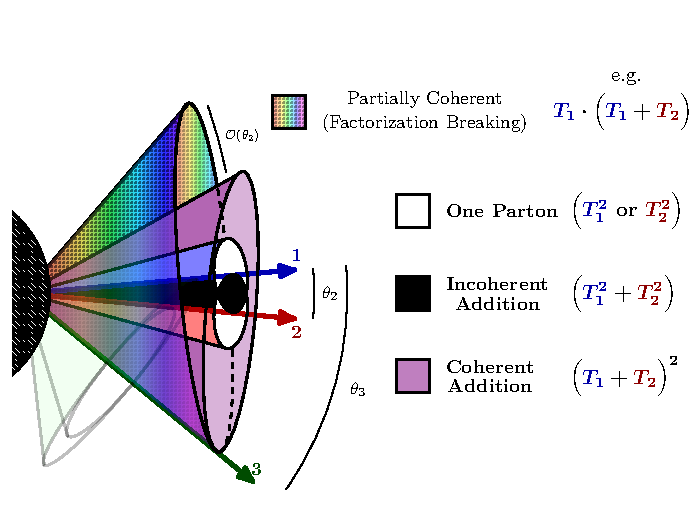
\includegraphics[width=1.05\textwidth]{figures/misc/color_coherence.pdf}
    \caption[A diagram illustrating color coherence and angular ordering in QCD.]
    {
        A diagram illustrating the first stage of color coherence and angular ordering in \gls{qcd}, whose recursive application leads to \Lem{qcd-coherent-branching}.
        %
        Near either individual parton \(i\in\{1,2\}\), soft gluons are emitted with a probability proportional to the \(T_i^2 = C_{R_i}\);
        %
        the overlap in which these probabilities add is striped red and blue.
        %
        However, in the region surrounding \emph{both} partons, indicated in purple, their charges add coherently and soft gluons are emitted with a probability proportional to \(C_{R_1\oplus R_2}\).
        %
        Beyond the collinear limit, a factorization-breaking \emph{fringe} (indicated as rainbow-colored and dotted) emerges around the coherent region, where it is less meaningful to talk about the probability of emitting a soft gluon;
        %
        in this region, the total differential cross section \(\dd\sigma_{N+1}\) \emph{does not factorize} into the product of an \(N\) particle differential cross section \(\dd\sigma_{N}\) and a soft gluon emission probability.
    }
    \label{fig:qcd-coherent-branching}
\end{figure}

\remark{}{
    Notably, \Lem{collinear-color-coherence} reproduces the factor of \(2 C_R \,\, \dd z/z \,\,\dd\theta/\theta\) that we saw emerge with our depth computations of splitting functions from \Secs{collinear-phase-space}{splitting-functions}.
    %
    It is encouraging that the soft limit for our explicit answers for soft gluon emission agree with the result guaranteed by \Thm{soft-gluon}.
    %
    To improve the accuracy of the results we obtain with \Thm{soft-gluon}, we can therefore replace the factor of \(2 C_R \dd \omega / \omega\) by \(P_{ij \leftarrow \ell}(z) \dd z\);
    %
    the splitting functions we derived do not change the behavior of the soft limit above -- any terms they add are subleading to the dominant \(1/z\) term -- but they \emph{also} capture universal behavior of partonic radiation in the purely collinear limit.
}



The tools we have explored in the proof of \Lem{collinear-color-coherence}, and the discussion of its recursion in the QED examples of \Example{charge-coherence} and \Exercise{charge-coherence-mparticle}, give us enough tools to take the next step and make a recursive statement in \gls{qcd}.
%
This may sound intimidating, but is not that bad.
%
Now that we know how the color indices work, everything really behaves structurally similar to the examples in QED -- the new feature is just that when our approximations fail, strict factorization also fails due to color correlations.
%
But we will not consider how.
%
We will pretend (however falsely) that our approximations -- the (recursive) collinear limits we used for coherent branching in QED -- always hold.
%
Now that you are completely absolved of blame for these approximations, I invite you to try the \gls{qcd} calculation yourself -- I really do think it is quite fun.

\begin{exercise}
    \label{ex:qcd-coherent-branching-proof}
    Don't get intimidated by the Lemma below.
    %
    Instead, by following the fixed-order logic of \Lem{collinear-color-coherence} and \Example{charge-coherence}, and the recursive logic of \Exercise{charge-coherence-mparticle} in the limit of a hierarchy of collinear splittings, demonstrate the phenomenon of \vocab{QCD Coherent Branching} (see also \Fig{qcd-coherent-branching}):
\end{exercise}


\begin{lemma}{Coherent Branching}{coherent-branching}
    Consider \(M\) outgoing particles, and an additional soft gluon, in the \vocab{strongly-angular-ordered limit}:%
    \footnote{
        Using the triangle equality, we could also write
        \(
            \theta_{12} \ll \theta_{(12)3} \ll \theta_{(123)4} \ll \cdots
            \,,
        \)
        where \(\theta_{(S)\,\,n}\) is the angle between \(\sum_{i\in S} \vec{k}_i\) and \(\vec{k}_n\).
    }
    \begin{align}
        \theta_{2} \ll \theta_{3} \ll \theta_{4}
        \ll
        \cdots
        \ll
        \theta_M
        \,,
    \end{align}
    where we define \(\theta_j = \theta_{1j}\) to be the angle of particle \(j\) relative to particle 1 for brevity.

    Finally, let \(\theta = \theta_{1q}\) be the angle of the soft gluon relative to particle 1.


    Then, up to terms which vanish in the limit of strong angular ordering, the emission of a soft gluon in a region around particle has the phase space distribution
    \begin{align}
        \label{eq:qcd-coherent-branching}
        \dsigmatilde
        \approx
        4 \as
        \,
        \frac{\dd E_q}{E_q}
        \,
        \frac{\dd \theta_q}{\theta_q}
        \,\,\,
        {\scriptscriptstyle\times}
        \,\,
        \begin{cases}
            C_{R_1}
            & \theta < \theta_{2}
            \\
            C_{R_{(12)}}
            & \theta_{2} \lesssim \theta \lesssim
            \theta_{3}, \theta_{(12)3}
            \\[2ex]
            \quad
            \vdots
            &
            \\[2ex]
            C_{R_{(12\,\cdots\,M-1)}}
            & \theta_{M-1} \lesssim \theta \lesssim
            \theta_{M}, \theta_{(1\cdots M-1)M}
            \,,
        \end{cases}
    \end{align}
    where the \(\lesssim\) is an unambiguous inequality in the strongly-angular-ordered limit, and \(R_{(1\cdots m)} := R_1 \oplus R_2 \oplus \cdots \oplus R_m\) is the representation formed by the direct sum of the representations of particles 1 through \(m\), which has generators (in a tensor product basis)
    \begin{align}
        \le(T^a_{(1\cdots m)}\ri)\indices{^{r_1\,\cdots\,r_m}_{r'_1\,\cdots\,r'_m}}
        \,\,
        :=&
        \,\,
        \le(T^a_{R_1}\ri)\indices{^{r_1}_{r'_1}}
        \,
        \delta\indices{^{r_2}_{r'_2}}\,\cdots\,\delta\indices{^{r_m}_{r'_m}}
        \,\,
        +
        \,\,
        \delta\indices{^{r_1}_{r'_1}}
        \le(T^a_{R_2}\ri)\indices{^{r_2}_{r'_2}}
        \delta\indices{^{r_3}_{r'_3}}\,\cdots\,\delta\indices{^{r_m}_{r'_m}}
        \notag
        \\
        &\qquad
        \,\,
        +
        \,\,
        \cdots
        \,\,
        +
        \delta\indices{^{r_1}_{r'_1}}
        \cdots
        \delta\indices{^{r_{m-1}}_{r'_{m-1}}}
        \le(T^a_{R_m}\ri)\indices{^{r_m}_{r'_m}}
        \,.
    \end{align}
\end{lemma}



We now cool it with the heat.
%
The remainder of the thesis will be less formal and exhausting about foundational results (though I may still advise you take a water break before \Sec{everything-on-shell}).



% ----------------------------------------------
\section{Substructure Diagrams and Fixed-Order Distributions}
% ----------------------------------------------
\label{sec:fixed-order-substructure}

We are finally ready to do some computations which reveal aspects of the internal structure of QCD partons.
%
In this section, we briefly introduce an important calculational tool for our analysis of jet substructure.
%
Before using the results of \Sec{universal-features} to recursively reveal the all-orders structure of jets -- the goal of our next chapter -- we take this opportunity to give results which are valid at \(\mathcal{O}(\alpha_s)\).
%
In \Chap{jets}, we will revisit these computations in the context of \textit{\glspl{jet}}, the beautiful formalism of the partonic cascade in order to obtained \textit{resummed} perturbative predictions which include corrections to arbitrary orders in \(\alpha_s\).


In this thesis, many of the observables we consider will be IRC safe and depend mostly on the less-energetic branch of a partonic splitting, such as mass \glspl{angularity} and \glspl{gecf}.
%
For example, the mass-squared associated with the splitting of a single parton is approximately \(m^2 = z(1-z)(1-\cos\theta) \approx \min(z, 1-z) \theta^2\), since, as shown in \Sec{universal-features}, the phase space of \gls{qcd} is dominated by singularities at which \(z\to 0\) or \(z \to 1\).
%
We call \(\min(z, 1-z)\) the \textit{soft energy fraction}.

The distribution of the angle and soft energy fraction of the splitting of a parton of flavor \(i\) is described in the \gls{collinear-limit} at \(\mathcal{O}(\alpha_s)\) by
%
\begin{align}
    \label{eq:emission-probability}
    \rho_{i}(z,\theta)
    &=
    \frac{\alpha_s}{\pi}
    \le[\bar{p}_i(z)\ri]^{(1/2)}_+ \frac{1}{\theta}
    ,
\end{align}
where \(z\in(0, 1/2)\) and \([\bar{p}(z)]^{(1/2)}_+ = [p(z) + p(1-z)]^{(1/2)}_+\) is a \glslink{plus-fn}{plus-regularized} \gls{redsplitfn}:
%
a modification of the full splitting function encoding only the energy fraction of the softer branch of the splitting.%
\footnote{
   If we would like to deal with observables which do not depend only on the softer energy fraction, we would need to work with a full (\glslink{plus-fn}{plus-regulated}) splitting function \([p(z)]^{(1)}_+\).
}

We will now use our technology to examine the fixed-order behavior of \glspl{observable} involving \textit{jets}.
%
Jets will be discussed in detail in \Chap{jets}, but for now we simply take them to be a collinear configuration of partons with limited angular separation \(\theta < \Rjet\).
%
Using \Eq{emission-probability}, the \(\mathcal{O}(\alpha_s)\) cumulative distribution of an observable \(X\) within a jet initiated by a parton of flavor \(i\) can be quickly represented as
\begin{align}
    \label{eq:cml-fixed-order}
    \Sigma_X(x)
    =
    \int
    \dd \theta
    \,
    \dd z
    \,
    \rho_{i}(z,\theta)
    \,\,
    \Theta(x > X(z, \theta))
    \,
    =
    \,
    \int
    \frac{\dd \theta}{\theta}
    \,
    \frac{\alpha_s}{\pi}
    \,
    \dd z
    \,
    \le[\bar{p}_i(z)\ri]^{(1/2)}_+
    \,
    \frac{\alpha_s}{\pi}
    \,\,
    \Theta(x > X(z, \theta))
    \,,
\end{align}
where we are abusing notation by writing \(X(z, \theta)\) to indicate the observable associated with a pair of momenta separated by an angle \(\theta\) and which carry fractions \(z\) and \((1-z)\) of the momenta of the full jet.


The definition of \glslink{plus-fn}{plus-regularization} yields
\begin{align}
    \int_0^{1/2} \dd z \le[\bar{p}(z)\ri]^{(1/2)}_+ g(z)
    =
    \int_0^{1/2} \dd z \,\, \bar{p}(z) \le(g(z) - g(0)\ri)
    \,,
\end{align}
assuming (correctly) that \(p(z)\) is only singular when \(z = 0\).
%
\begin{subequations}
Using also that \(\Theta(a) = 1 - \Theta(-a)\), we can therefore re-write \Eq{cml-fixed-order} as
\begin{align}
    \Sigma_X(x)
    \,
    &=
    \,
    \int
    \frac{\dd \theta}{\theta}
    \,
    \dd z
    \,
    \le[\bar{p}_i(z)\ri]^{(1/2)}_+
    \,
    \frac{\alpha_s}{\pi}
    \,\,
    \le(
        1 - \Theta(X(z, \theta) > x)
    \ri)
    \\
    &=
    \,
    \int
    \frac{\dd \theta}{\theta}
    \,
    \dd z
    \,
    \bar{p}_i(z)
    \,
    \frac{\alpha_s}{\pi}
    \,\,
    \le(
        -\Theta(X(z, \theta) > x)
        +\Theta(X(0, \theta) > x)
    \ri)
    \,.
\end{align}
%
The observables we consider in this thesis, such as masses and angularities, have \(X\big|_{z=0} = 0\), so that \(X(0, \theta) < x\) for any finite \(x\)
%
Therefore, we may write, at least for \(x > 0\), that
\begin{align}
    \label{eq:cml-fixed-order-veto}
    \Sigma_X(x)
    \,
    &=
    \,
    -
    \int
    \frac{\dd \theta}{\theta}
    \,
    \dd z
    \,
    \bar{p}_i(z)
    \,
    \frac{\alpha_s}{\pi}
    \,\,
    \Theta(X(z, \theta) > x)
    \,.
\end{align}
%
\end{subequations}


\remark{}{
    The region of phase space in which an emission contributes a value greater than \(x\) to the observable \(X\) -- i.e. where \(X(z, \theta) > x\) -- is called a \vocab{\gls{vetoreg}}.
    %
    \Eq{cml-fixed-order-veto} therefore expresses the cumulative distribution for \(X\) as the integral of the phase space density \(\rho_i(z, \theta)\) over the veto region.
    %
    The integral of \(\rho_i(z,\theta)\) over the \gls{vetoreg} for an observable is also called the \vocab{\gls{radiator}} \(R_X(x)\) for the observable.
    %
    The radiator will reappear in our calculations of resummed quantities in \Chap{jets}, and modified definitions will even capture the effects of multiple emissions and the running coupling of QCD.
}


The integral of \Eq{cml-fixed-order} captures the probability that a jet contains a single emission which lies in a particular region of phase space.
%
We will represent such integrals in terms of \vocab{\glspl{substructure-diagram}}:

\begin{definitionbox}{Substructure Diagram}{substructure-diagram}
    A \emph{\gls{substructure-diagram}} is a graphical representation that the probability of a splitting whose angle \(\theta\) and softer energy fraction \(z\) lie within some region of phase space.

    \vspace{7pt}
    \hrule
    \vspace{7pt}

    \vocab{Substructure diagrams} describe the probability of finding a splitting in some region in the \(\log(z^{-1})\)-\(\log(\theta^{-1})\) plane, or Lund plane, with a diagram of the Lund plane with the corresponding region filled:
%
\begin{align}
    \iint_{
    
\begin{tikzpicture}[scale=.06]
    \begin{axis}
    [xmin=0, xmax=5,
    ymin=0, ymax=5,
    axis line style = {draw=none},
    ticks=none]
    	\draw[blue, line width=9pt, fill=blue,fill opacity=0.3] \pgfextra{
    	  \pgfpathellipse{\pgfplotspointaxisxy{2.5}{2.5}}
    		{\pgfplotspointaxisdirectionxy{0}{1.8}}
        	{\pgfplotspointaxisdirectionxy{1.2}{.5}}
    	};
    \end{axis}
    \end{tikzpicture}
    }
    \frac{\alpha_s}{\pi}~
    \frac{\dd\theta}{\theta}~
    \dd z~
    [\bar{p}_i(z)]^{(1/2)}_+
    ~~~
    \triangleq
    ~~~
    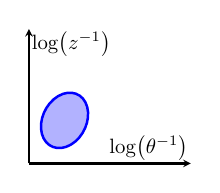
\begin{tikzpicture}[
    baseline={([yshift=-.8ex]current bounding box.center)},
    vertex/.style={anchor=base,
    circle,fill=black!25,minimum size=18pt,inner sep=2pt},
    scale=.3]
    \begin{axis}
    [
    xlabel=\scalebox{2.5}
    {\(\log(\theta^{-1})\)},
    ylabel=\scalebox{2.5}
    {\(\log(z^{-1})\)},
    xmin=0, xmax=5,
    ymin=0, ymax=5,
    axis line style = {line width=3pt},
    axis y line*=left,
    axis x line*=bottom,
    axis lines = middle,
    ticks=none]
    	\draw[blue, line width=3pt, fill=blue,fill opacity=0.3]
    	\pgfextra{
    	  \pgfpathellipse{\pgfplotspointaxisxy{1.1}{1.6}}
    		{\pgfplotspointaxisdirectionxy{-.2}{.9}}
    		{\pgfplotspointaxisdirectionxy{.7}{.5}}
    	};
    \end{axis}
    \end{tikzpicture}
    ~~~
    \triangleq
    ~~~
    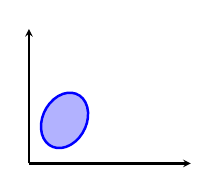
\begin{tikzpicture}[
    baseline={([yshift=-.8ex]current bounding box.center)},
    vertex/.style={anchor=base,
    circle,fill=black!25,minimum size=18pt,inner sep=2pt},
    scale=.3]
    \begin{axis}
    [xmin=0, xmax=5,
    ymin=0, ymax=5,
    axis line style = {line width=3pt},
    axis y line*=left,
    axis x line*=bottom,
    axis lines = middle,
    ticks=none]
    	\draw[blue, line width=3pt, fill=blue,fill opacity=0.3]
    	\pgfextra{
    	  \pgfpathellipse{\pgfplotspointaxisxy{1.1}{1.6}}
    		{\pgfplotspointaxisdirectionxy{-.2}{.9}}
    		{\pgfplotspointaxisdirectionxy{.7}{.5}}
    	};
    \end{axis}
    \end{tikzpicture}
    ,
\end{align}
where the shaded oval in the Lund plane above represents an arbitrary shape associated with a region of two-particle phase space.
\end{definitionbox}


\remark{}{
It follows, for example, that
%
\begin{align}
    \label{eq:plus-fn-diagram-identities}
    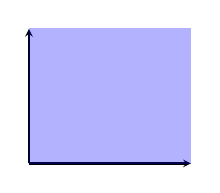
\begin{tikzpicture}[
    baseline={([yshift=-.8ex]current bounding box.center)},
    vertex/.style={anchor=base,
    circle,fill=black!25,minimum size=18pt,inner sep=2pt},
    scale=.3]
    \begin{axis}
    [xmin=0, xmax=5,
    ymin=0, ymax=5,
    axis line style = {line width=3pt},
    axis y line*=left,
    axis x line*=bottom,
    axis lines = middle,
    ticks=none]
    	\draw[blue, line width=3pt, fill=blue,fill opacity=0.3]
    	\pgfextra{
    	  \pgfpathellipse{\pgfplotspointaxisxy{0}{0}}
    		{\pgfplotspointaxisdirectionxy{0}{100}}
    		{\pgfplotspointaxisdirectionxy{100}{0}}
    	};
    \end{axis}
    \end{tikzpicture}
    =
    0
    ~~~~~~~~~
    {\rm and}
    ~~~~~~~~~
    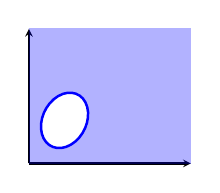
\begin{tikzpicture}[
    baseline={([yshift=-.8ex]current bounding box.center)},
    vertex/.style={anchor=base,
    circle,fill=black!25,minimum size=18pt,inner sep=2pt},
    scale=.3]
    \begin{axis}
    [xmin=0, xmax=5,
    ymin=0, ymax=5,
    axis line style = {line width=3pt},
    axis y line*=left,
    axis x line*=bottom,
    axis lines = middle,
    ticks=none]
    	\draw[blue, line width=3pt, fill=blue,fill opacity=0.3]
    	\pgfextra{
    	  \pgfpathellipse{\pgfplotspointaxisxy{0}{0}}
    		{\pgfplotspointaxisdirectionxy{0}{100}}
    		{\pgfplotspointaxisdirectionxy{100}{0}}
    	};
    	\draw[blue, line width=3pt, fill=white,fill opacity=1.0]
    	\pgfextra{
    	  \pgfpathellipse{\pgfplotspointaxisxy{1.1}{1.6}}
    		{\pgfplotspointaxisdirectionxy{-.2}{.9}}
    		{\pgfplotspointaxisdirectionxy{.7}{.5}}
    	};
    \end{axis}
    \end{tikzpicture}
    ~~
    =
    ~~
    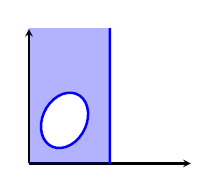
\begin{tikzpicture}[
    baseline={([yshift=-.8ex]current bounding box.center)},
    vertex/.style={anchor=base,
    circle,fill=black!25,minimum size=18pt,inner sep=2pt},
    scale=.3]
    \begin{axis}
    [xmin=0, xmax=5,
    ymin=0, ymax=5,
    axis line style = {line width=3pt},
    axis y line*=left,
    axis x line*=bottom,
    axis lines = middle,
    ticks=none]
    	\draw[blue, line width=3pt, fill=blue,fill opacity=0.3]
    	\pgfextra{
    	  \pgfpathellipse{\pgfplotspointaxisxy{0}{.9}}
    		{\pgfplotspointaxisdirectionxy{0}{200}}
    		{\pgfplotspointaxisdirectionxy{2.5}{.9}}
    	};
    	\draw[blue, line width=3pt, fill=white,fill opacity=1.0]
    	\pgfextra{
    	  \pgfpathellipse{\pgfplotspointaxisxy{1.1}{1.6}}
    		{\pgfplotspointaxisdirectionxy{-.2}{.9}}
    		{\pgfplotspointaxisdirectionxy{.7}{.5}}
    	};
    \end{axis}
    \end{tikzpicture}
    ~~
    =
    ~~
    -~
    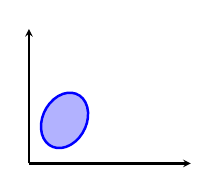
\begin{tikzpicture}[
    baseline={([yshift=-.8ex]current bounding box.center)},
    vertex/.style={anchor=base,
    circle,fill=black!25,minimum size=18pt,inner sep=2pt},
    scale=.3]
    \begin{axis}
    [xmin=0, xmax=5,
    ymin=0, ymax=5,
    axis line style = {line width=3pt},
    axis y line*=left,
    axis x line*=bottom,
    axis lines = middle,
    ticks=none]
    	\draw[blue, line width=3pt, fill=blue,fill opacity=0.3]
    	\pgfextra{
    	  \pgfpathellipse{\pgfplotspointaxisxy{1.1}{1.6}}
    		{\pgfplotspointaxisdirectionxy{-.2}{.9}}
    		{\pgfplotspointaxisdirectionxy{.7}{.5}}
    	};
    \end{axis}
    \end{tikzpicture}
    .
\end{align}
As depicted above, we may replace any vertical line -- representing an integral over \(z\) at fixed \(\theta\) -- or any vertical strip -- representing an integral over \(z\) and some range of \(\theta\) -- with zero, since the integral of a \gls{plus-fn} is zero.
}



\begin{example}
    \label{ex:mass-fixed-order}
    The pairwise mass of two massless partons emerging from a single splitting is given by
    \begin{equation}
    \begin{aligned}
        m^2 &= (p_1 + p_2)^2 = 2 p_1 \cdot p_2
        =
        2 Q^2
        \,
        z \, (1-z)
        \le(1 - \cos(\theta)\ri)
        \\
        &\approx
        Q^2 z \theta^2
        .
    \end{aligned}
    \end{equation}

    Therefore, in a jet of radius \(\Rjet\), the corresponding \gls{substructure-diagram} showing the veto region \(z\theta^2 > m^2 / Q^2\) is
    \begin{center}
    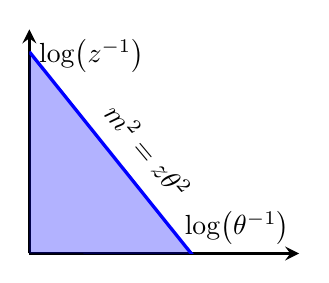
\begin{tikzpicture}[scale=0.5]
    \begin{axis}
    [xlabel=\(\log(\theta^{-1})\), ylabel=\(\log(z^{-1})\),
    xmin=0, xmax=5,
    ymin=0, ymax=5,
    axis line style = very thick,
    axis y line*=left,
    axis x line*=bottom,
    axis lines = middle,
    ticks=none]
        \addplot[name path=f,domain=0:5,
        style=very thick,blue]
        {4.5-1.5*x};

        \path[name path=axis]
        (axis cs:0,0) -- (axis cs:1,0);

        \addplot [
            thick,
            color=blue,
            fill=blue,
            fill opacity=0.3
        ]
        fill between[
            of=f and axis
        ];

        \node [rotate=-50] at (axis cs:  2.2,  2.3) {$m^2 = z\theta^2$};
    \end{axis}
    \end{tikzpicture}
    \end{center}

    We can easily read off the resummed distribution for the mass squared of a jet at the level of accuracy we are pursuing (leaving the integrals to you):
    \begin{align}
        \Sigma(m^2)
        \approx
        -
        \,\,\,
        \raisebox{-10pt}{
        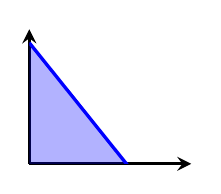
\begin{tikzpicture}[
        baseline={([yshift=-.8ex]current bounding box.center)},
        vertex/.style={anchor=base,
        circle,fill=black!25,minimum size=18pt,inner sep=2pt},
        scale=.3]
        \begin{axis}
        [xmin=0, xmax=5,
        ymin=0, ymax=5,
        axis line style = very thick,
        axis y line*=left,
        axis x line*=bottom,
        axis lines = middle,
        ticks=none]
        	\addplot[name path=f,domain=0:5,
            style=very thick,blue]
            {4.5-1.5*x};
            \path[name path=axis]
            (axis cs:0,0) -- (axis cs:1,0);
            \addplot [
                thick,
                color=blue,
                fill=blue,
                fill opacity=0.3
            ]
            fill between[
                of=f and axis
            ];
        \end{axis}
        \end{tikzpicture}
        }
        =
        -
        \frac{\alpha_{\rm S}}{\pi}
        \iint_{z\theta^2 > m^2}
        \dd\log(\theta) ~~ \dd z ~ [p(z)]_+
    \end{align}

    Plugging in the leading, singular piece for the splitting function at leading logarithmic accuracy, \(p(z) \sim 2 C_R / z\) for a splitting initiated by a parton with \(SU(3)\) color representation \(R\), and putting back in factors of \(Q\), we find
    \begin{align}
        \Sigma(m^2)
        \approx
        -\frac{C_R\alpha_{\rm S}}{2 \pi}\log^2\left(\frac{m^2}{Q^2}\right)
        \,,
    \end{align}
    with the associated pseudo-probability density
    \begin{align}
        \rho(m^2)
        =
        \frac{\dd}{\dd m^2} \Sigma(m^2)
        \approx
        \frac{C_R \alpha_s}{\pi}
        \frac{1}{m^2}
        \log\le(\frac{Q^2}{m^2}\ri)
        \,.
    \end{align}

    This describes the mass-squared distribution for a two-particle final state in the \gls{collinear-limit}.
    %
    We will include the effects of many emissions in \Sec{ll-substructure-diagrams} of \Chap{jets}.
\end{example}
~\\

\begin{exercise}{}
    Repeat the analysis of Example \ref{ex:mass-fixed-order} above with and without \glspl{substructure-diagram} for the leading pieces of the NLO distributions of \glspl{angularity} \(e_\varsigma\) (\Eq{angularitydefn_lo}) and \glspl{gecf} \(C_1^{(\varsigma)}\) (\Eq{GECFdefn_lo}).
    %
    I find
    \begin{align}
        \Sigma_{\le(e_\varsigma\ri)}(x)
        \approx
        \Sigma_{\le(C_1^{(\varsigma)}\ri)}(x)
        \,\,
        &\approx
        \,\,
        -\frac{C_R\alpha_{\rm S}}{\varsigma \pi}\log^2(x)
        \\
        \rho_{\le(e_\varsigma\ri)}(x)
        \approx
        \rho_{\le(C_1^{(\varsigma)}\ri)}(x)
        \,\,
        &\approx
        \,\,
        -\frac{C_R\alpha_{\rm S}}{\varsigma \pi} \frac{1}{x}
        \log\left(x\right)
        \,.
    \end{align}
    Compare these two results to the mass distribution of a partonic splitting obtained in \Example{mass-fixed-order}.

    Argue that all three may be plus-regularized (as discussed in the context of splitting functions in \Sec{splitting-functions}) to yield a normalized distribution, though not a probability distribution.
\end{exercise}




% ==============================================
\section{Connecting back out}
% ==============================================

In this chapter, we have explored the framework of scattering and quantum field theory used by particle physicists to explore the subatomic universe.
%
Our discussions and derivations of the universal, fixed-order features of \gls{qcd} gave us quantitative tests of \gls{qcd} scattering.
%
We saw a hint of something deeper, however:
%
we may hope to push beyond fixed order predictions by repeated application of soft theorems and angular ordering.
%
We pursue a more rigorous understanding of this recursive, fractal-like nature of \gls{qcd} radiation in the next chapter, where we will discover and quantify the intricate features of jets.



\begin{subappendices}

\section{A Collinear QCD Compendium}
\label{app:qcd-compendium}

\subsection{Gluons and Polarization Vectors}

Polarization vectors are a tricky business -- the transformation properties of polarizations are inextricably linked with gauge invariance.%
\footnote{
    see Weinberg's \underline{The Theory of Quantum Fields, Volume I}, Chapter 2.5 \cite{Weinberg:1995mt} and especially Matthew Schwartz' \underline{Quantum Field Theory and the Standard Model}, Chapter 8.4.2 \cite{Schwartz:2014sze}.
}
%
As we saw in \Sec{splitting-functions}, where Ward identities did not apply, we have to be careful in computations with off-shell legs, and the mixing of the properties of polarizations and gauge-invariance can be confusing.

However, we can pick convenient bases for the physical polarization vectors of gluons.
%
For a spin-one gauge boson moving along the \(z\)-axis, \(p^\mu - E_p \le(1,0,0,1\ri)\), a canonical basis for the polarization vectors is the pair
\begin{subequations}
\label{eq:z-polarization}
\begin{align}
    \varepsilon^\mu_{+,\,z}
    &\reppedby
    \frac{1}{\sqrt{2}}
    \le(0, 1, -i, 0\ri)
    \\
    \varepsilon^\mu_{-,\,z}
    &\reppedby
    \frac{1}{\sqrt{2}}
    \le(0, 1, +i, 0\ri)
    \,,
\end{align}
\end{subequations}
with the notable property that
\begin{align}
    \varepsilon_\lambda \cdot \varepsilon_{\lambda'}^*
    =
    \delta_{\lambda \lambda'}
    \,.
\end{align}


\begin{exercise}
    Show that \(p\cdot \epsilon = 0\) for the polarization four-vectors of \Eq{z-polarization}, and furthermore that they are eigenvectors of the \textit{little group transformations} -- Lorentz transformations which leave the momentum \(p^\mu\) invariant -- consisting of rotations about the \(z\)-axis represented by the matrix \(\Lambda(\phi)\)%
    \footnote{
        These rotations are not the only little group transformations for our massless gluon, but they are the only ones that matter;
        %
        see Weinberg's \underline{The Theory of Quantum Fields, Volume I}, Chapter 2.5 \cite{Weinberg:1995mt}.
    }:
    \begin{align}
        \Lambda\indices{^\mu_\nu}(\phi) \varepsilon^\nu_{\pm,\,z}
        =
        e^{\pm i \phi} \varepsilon^\mu_{\pm,\,z}
        \,.
    \end{align}
\end{exercise}



A constructive way of producing polarization vectors for general momenta is by selecting two arbitrary four-vectors, projecting each to the component orthogonal to the gauge-boson four-momentum \(p^\mu\) (Mathematica's \texttt{Orthogonalize} is a useful tool), and then finding the orthogonal linear combinations which are eigenvectors of the little group rotations of \(p^\mu\).
%
For the calculations of splitting functions in this section,
%(and for the calculation of the QED polarization vectors in \Prob{massless-qed}),
we now record the results for polarization vectors of collinear gluons.

\begin{example}
In the concrete calculations of splitting functions in \Sec{splitting-functions}, we will also need polarization vectors for \textit{collinear} gluons travelling nearly along the \(z\)-axis, with a polar angle \(\theta \ll 1\):
\begin{align}
    k^\mu =
    E_k
    \le(1,\, \sin\theta\cos\phi,\, \sin\theta\sin\phi,\,\cos\theta\ri)
    =
    E_k
    \le(1,\, \theta\cos\phi,\, \theta\sin\phi,\,1 - \theta^2/2\ri)
    +
    \mathcal{O}(\theta^3)
    \,.
\end{align}
A convenient basis for the associated polarization vectors in our collinear limit calculations is
\begin{align}
    \label{eq:collinear-polarization}
    \varepsilon^\mu_\lambda(k)
    \approx
    \varepsilon^\mu_\lambda
    -
    \frac{e^{-i\lambda \phi}}{\sqrt{2}}
    \le(
    \frac{\theta^2}{2}\cos\phi,\,
    \frac{\theta^2}{2}\sin\phi,\,
    \theta
    \ri)
    \,,
\end{align}
where \(\lambda \in \{+,-\}\).
\end{example}

\begin{exercise}
    Show that the collinear-limit polarization vectors of \Eq{collinear-polarization} are orthogonal to the collinear momentum \(k^\mu\) and are mutually orthonormal, at \(\mathcal{O}(\theta^2)\).
\end{exercise}




\subsection{Quarks and Polarization Bi-Spinors}

A full Lorentz- and parity-invariant description of fermions in \(d = 3+1\) dimensions requires the use of \textit{gamma matrices}, satisfying
\begin{align}
    \acomm{\gamma^\mu}{\gamma^\nu} = -2 g^{\mu\nu}
    \,.
\end{align}
%
In the concrete calculations of this work, we will use the \textit{chiral} basis for the gamma matrices:
\begin{align}
    \gamma^\mu = \pmtrx{0 & \sigma^\mu\\\overline{\sigma}^\mu & 0}
    \,,
\end{align}
where \(\sigma^\mu = (1, \vec{\sigma})\) and \(\overline{\sigma}^\mu = (1, -\vec{\sigma})\) are invariant symbols of the Lorentz group.


\begin{example}
    \label{ex:collinear-kslash}
    Consider a massless particle with momentum \(k_1^\mu\) moving at a polar angle \(\theta_1\) relative to the \(z\) axis and an azimuthal angle \(\phi_1\) in the \(x\)-\(y\) plane.
    %
    Its momentum is \(k^\mu \reppedby E_1 \le(1, \sin\theta_1\cos\phi_1, \sin\theta_1 \sin\phi_1,\cos\theta_1\ri)\), and therefore
    \begin{align}
        \slashed{k}_1
        :=
        k_1^\mu \gamma_\mu
        &=
        E_1 \pmtrx{0 & 1 - \vec{k}\cdot \vec{\sigma} \\ 1 +  \vec{k}\cdot \vec{\sigma} & 0}
        \\
        &=
        E_1
        \pmtrx{
            0&0&1 - \cos\theta_1& -\sin\theta_1 e^{-i\phi_1}
            \\
            0&0& -\sin\theta_1 e^{i\phi_1} & 1 + \cos\theta_1
            \\
            1 + \cos\theta_1 & \sin\theta_1 e^{-i\phi_1} & 0 & 0
            \\
            \sin\theta_1 e^{i\phi_1} & 1 - \cos\theta_1 & 0 & 0
        }
        \,.
    \end{align}
    In the collinear limit where \(\theta_1 \ll 1\), as we often consider in this thesis, we can therefore write
    \begin{align}
        \slashed{k}_1
        =
        E_1
        \pmtrx{
            0&0& \theta_1^2/2 & -\theta_1 e^{-i\phi_1}
            \\
            0&0 & -\theta_1 e^{i\phi_1} & 2 - \theta_1^2/2
            \\
            2 - \theta_1^2/2 & \theta_1 e^{-i\phi_1} & 0 & 0
            \\
            \theta_1 e^{i \phi_1} & \theta_1^2/2 & 0 & 0
        }
        +
        \mathcal{O}\le(\theta_1^3\ri)
        \,.
    \end{align}
    This expression is useful for several of the concrete computations of this chapter.
\end{example}



In this basis, spinor factors take the form
\begin{subequations}
\begin{align}
    \label{eq:bispinor-u}
    u_s(p)
    &=
    \pmtrx{
        \sqrt{p\cdot \sigma}\ket{s}
        \\
        \sqrt{p\cdot{\overline{\sigma}}} \ket{s}
    }
    \\
    \label{eq:bispinor-v}
    v_s(p)
    &=
    \pmtrx{
        \sqrt{p\cdot \sigma}\sigma_x \ket{s}
        \\
        -\sqrt{p\cdot{\overline{\sigma}}} \sigma_x \ket{s}
    }
    =:
    \pmtrx{
        \sqrt{p\cdot \sigma}\ket{\overline{s}}
        \\
        -\sqrt{p\cdot{\overline{\sigma}}} \ket{\overline{s}}
    }
    \,,
\end{align}
\end{subequations}
where we have abused notation by using \(\ket{s}\) to denote the 2-spinor encoding the particle's spin measured in the \(\sigma_z\)/``computational'' basis.
%
In particular
\begin{align}
    \ket{s}
    =
    \begin{cases}
        \pmtrx{1\\0}
        &
        s = +
        \quad \leftrightarrow \quad
        \text{spin } s \text{ is along } +\hat{z}
        \,,
        \\
        \pmtrx{0\\1}
        &
        s = -
        \quad \leftrightarrow \quad
        \text{spin } s \text{ is along } -\hat{z}
        \,.
    \end{cases}
\end{align}

For a four-component spinor \(\psi\) (such as \(u_s(p)\) or \(v_s(p)\)) \(\bar{\psi}\) is defined by
\begin{align}
    \bar{\psi} := \psi^\dagger \gamma^0
    \,,
\end{align}


\begin{example}
    \label{eq:massive-bispinor}
    Consider a massive spin-1/2 particle moving in the \(z\)-direction with energy \(E_P\) and momentum \(\vec{P} = P \hat{z}\) along the \(z\)-axis.
    %
    Using our suboptimal metric signature (\(g = \text{diag}(+,-,-,-)\)), we have
    \begin{align}
        p\cdot \sigma
        =
        \pmtrx{E_P - P & 0 \\ 0 & E_P + P}
        =:
        E_P \pmtrx{1 - \beta & 0 \\ 0 & 1 + \beta}
        \\
        p\cdot \overline{\sigma}
        =
        \pmtrx{E_P + P & 0 \\ 0 & E_P - P}
        =:
        E_P \pmtrx{1 + \beta & 0 \\ 0 & 1 - \beta}
        \,,
    \end{align}
    where \(\beta := P / E_P\) is the velocity of the particle;
    %
    we also have \(\beta^2 = 1 - m^2/E^2\).

    Therefore, using the Weyl basis for the gamma matrices, we may write
    \begin{align}
        \label{eq:bispinor-u-virtual}
        u_+(P)
        =
        \sqrt{E_P}
        \pmtrx{\sqrt{1-\beta}\\0\\\sqrt{1+\beta}\\0}
        \,,\qquad
        u_-(P)
        =
        \sqrt{E_P}
        \pmtrx{0\\\sqrt{1+\beta}\\0\\\sqrt{1-\beta}}
        \,,
        \\
        \label{eq:bispinor-v-virtual}
        v_+(P)
        =
        \sqrt{E_P}
        \pmtrx{0\\\sqrt{1+\beta}\\0\\-\sqrt{1-\beta}}
        \,,\qquad
        v_-(P)
        =
        \sqrt{E_P}
        \pmtrx{\sqrt{1-\beta}\\0\\-\sqrt{1+\beta}\\0}
        \,.
    \end{align}

    % In the high-energy limit \(\beta \approx 1 - m^2 / 2 E^2\), and
    % \begin{align}
    %     \label{eq:bispinor-u-high-energy}
    %     u_+(P)
    %     =
    %     \sqrt{2E_P}
    %     \pmtrx{m / 2 E_P \\0\\1\\0}
    %     ,\qquad
    %     u_-(P)
    %     =
    %     \sqrt{2 E_P}
    %     \pmtrx{0 \\ 1 \\0\\m / 2 E_P}
    %     \,,
    %     \\
    %     \label{eq:bispinor-v-high-energy}
    %     v_+(P)
    %     =
    %     \sqrt{2 E_P}
    %     \pmtrx{0\\1\\0\\-m/2E_P}
    %     ,\qquad
    %     v_-(P)
    %     =
    %     \sqrt{2 E_P}
    %     \pmtrx{m/2E_P\\0\\-1\\0}
    %     \,,
    % \end{align}
    % up to \(\mathcal{O}\le(\frac{m^2}{E^2}\ri)\) (approximation is instructive, but dropping these terms drops important e
\end{example}



\begin{exercise}
    Using \Eqs{bispinor-u}{bispinor-v}, show that \(\sum_s u_s(p) \bar{u}_s(p) = \slashed{p} + m\), and \(\sum_s v_s(p) \bar{v}_s(p) = \slashed{p} - m\).

    \vspace{7pt}
    \hrule

    \begin{center}
        \texttt{(Hint:)}

        Use \(\sum_s \ketbra{s}{s} = 1\).
    \end{center}
\end{exercise}



At high energies, or in the massless limit, the polarization bi-spinors take the form
\begin{subequations}
\label{eq:massless-four-component-spinors}
\begin{align}
    u_s(p)
    &=
    \sqrt{\frac{E_p}{2}}
    \pmtrx{
        \le(1 - \hat{p}\cdot \vec{\sigma}\ri)\ket{s}
        \\
        \le(1 + \hat{p}\cdot \vec{\sigma}\ri)\ket{s}
    }
    \\
    v_s(p)
    &=
    \sqrt{\frac{E_p}{2}}
    \pmtrx{
        \le(1 - \hat{p}\cdot \vec{\sigma}\ri) \ket{\overline{s}}
        \\
        -\le(1 + \hat{p}\cdot \vec{\sigma}\ri) \ket{\overline{s}}
    }
    \,,
\end{align}
where \(E_p = p^0\).
\end{subequations}

We note also that
\begin{align}
    \hat{p}\cdot\vec{\sigma}
    =
    \pmtrx{
        \cos\theta            &    \sin\theta e^{-i\phi}
        \\
        \sin\theta e^{i\phi}  &    -\cos\theta
    }
    \,,
\end{align}
where \(\theta\) is the polar angle of \(\hat{p}\) relative to the \(z\)-axis.



\begin{exercise}
    Verify \Eq{massless-four-component-spinors}.
    %
    Show that it implies \(\sum_s u_s \bar{u}_s = \sum_s v_s \bar{v}_s = \slashed{p}\).
\end{exercise}


\begin{example}
    \label{ex:collinear-bispinor}
    Finally, we take the limit in which a massless particle is nearly \glslink{collinear-limit}{collinear} with the \(z\)-axis, for which
    %
    \(
        p^\mu
        =
        E \le(1, \, \sin\theta \cos\phi, \, \sin\theta \sin\phi, \, \cos\theta\ri)
    \)
    %
    reduces to
    %
    \(
        p^\mu
        =
        E \le(1, \, \theta \cos\phi, \, \theta\sin\phi, \, 1 - \theta^2/2\ri)
        +
        \mathcal{O}(\theta^3)
    \).
    %
    In this limit, we have
    \begin{align}
        \hat{p}\cdot\vec{\sigma}
        \approx
        \pmtrx{1 - \theta^2/2& \theta e^{-i\phi} \\ \theta e^{i\phi} & -1+\theta^2/2}
        +
        \mathcal{O}(\theta^3)
        \,,
    \end{align}
    and accordingly, at \(\mathcal{O}(\theta^2)\),
    \begin{align}
        \label{eq:bispinor-u-collinear}
        u_+(p)
        =
        \sqrt{2 E_p}
        \pmtrx{\theta^2/4 \\ -\theta e^{i\phi}/2 \\ 1-\theta^2/4 \\ \theta e^{i\phi}/2}
        +
        \mathcal{O}(\theta^3)
        \,,
        \quad
        u_-(p)
        =
        \sqrt{2 E_p}
        \pmtrx{-\theta e^{-i\phi}/2 \\ 1 - \theta^2/4\\ \theta e^{-i\phi}/2 \\  \theta^2/4}
        +
        \mathcal{O}(\theta^3)
        \,,
        \\
        \label{eq:bispinor-v-collinear}
        v_+(p)
        =
        \sqrt{2 E_p}
        \pmtrx{-\theta e^{-i\phi}/2 \\ 1 - \theta^2/4\\ -\theta e^{-i\phi}/2 \\ -\theta^2/4}
        +
        \mathcal{O}(\theta^3)
        \,,
        \quad
        v_-(p)
        =
        \sqrt{2 E_p}
        \pmtrx{\theta^2/4\\ -\theta e^{i\phi}/2 \\ -1+\theta^2/4 \\ -\theta e^{i\phi}/2}
        +
        \mathcal{O}(\theta^3)
        \,.
    \end{align}
\end{example}


\begin{exercise}
    Verify that \(\sum_s u_s \bar{u}_s (p) = \sum_s v_s \bar{v}_s (p) = \slashed{p}\) at \(\mathcal{O}(\theta^2)\) for the collinear spinors above.
    % \Eqs{bispinor-square-u}{bispinor-square-v}.
    % Working to \(\mathcal{O}(\theta)\) for brevity, verify that
    % \begin{align}
    %     u_+\bar{u}_+(p)
    %     &=
    %     2 E_p
    %     \pmtrx{
    %         0 & 0 & 0 & 0 \\
    %         -\frac{1}{2} \theta  e^{i \phi } & 0 & 0 & 0 \\
    %         1 & \frac{1}{2} \theta  e^{-i \phi } & 0 &
    %         -\frac{1}{2} \theta  e^{-i \phi } \\
    %         \frac{1}{2} \theta  e^{i \phi } & 0 & 0 & 0
    %     }
    %     +
    %     \mathcal{O}(\theta^2)
    %     \,,
    %     \\
    %     u_-\bar{u}_-(p)
    %     &=
    %     2 E_p
    %     \pmtrx{
    %         0 & 0 & 0 & -\frac{1}{2} \theta  e^{-i \phi } \\
    %         \frac{1}{2} \theta  e^{i \phi } & 0 &
    %         -\frac{1}{2} \theta  e^{i \phi } & 1 \\
    %         0 & 0 & 0 & \frac{1}{2} \theta  e^{-i \phi } \\
    %         0 & 0 & 0 & 0
    %     }
    %     +
    %     \mathcal{O}(\theta^2)
    %     \,,
    %     \\
    %     v_+\bar{v}_+(p)
    %     &=
    %     \pmtrx{
    %         0 & 0 & 0 & -\frac{1}{2} \theta  e^{-i \phi } \\
    %         -\frac{1}{2} \theta  e^{i \phi } & 0 &
    %         -\frac{1}{2} \theta  e^{i \phi } & 1 \\
    %         0 & 0 & 0 & -\frac{1}{2} \theta  e^{-i \phi } \\
    %         0 & 0 & 0 & 0
    %     }
    %     +
    %     \mathcal{O}\le(\theta^2\ri)
    %     \,,
    %     \\
    %     v_-\bar{v}_-(p)
    %     &=
    %     \pmtrx{
    %         0 & 0 & 0 & 0 \\
    %         \frac{1}{2} \theta  e^{i \phi } & 0 & 0 & 0 \\
    %         1 & \frac{1}{2} \theta  e^{-i \phi } & 0 &
    %         \frac{1}{2} \theta  e^{-i \phi } \\
    %         \frac{1}{2} \theta  e^{i \phi } & 0 & 0 & 0 \\
    %         \frac{1}{2} \theta  e^{i \phi } & 0 & 0 & 0
    %     }
    %     +
    %     \mathcal{O}\le(\theta^2\ri)
    %     \,.
    % \end{align}

    % Checking terms to \(\mathcal{O}(\theta^2)\) (though higher-order terms agree as well), we find
    % \begin{align}
    %     \label{eq:bispinor-square-u}
    %     \sum_s u_s \bar{u}_s (p)
    %     &
    %     =
    %     2 E_p
    %     \pmtrx{
    %         0 & 0 & 0 & -\frac{1}{2} \theta  e^{-i \phi } \\
    %         0 & 0 & -\frac{1}{2} \theta  e^{i \phi } & 1 \\
    %         1 & \frac{1}{2} \theta  e^{-i \phi } & 0 & 0 \\
    %         \frac{1}{2} \theta  e^{i \phi } & 0 & 0 & 0
    %     }
    %     +
    %     \mathcal{O}\le(\theta^2\ri)
    %     \overset{\checkmark}{=}
    %     \slashed{p}
    %     \\
    %     \label{eq:bispinor-square-v}
    %     \sum_s v_s \bar{v}_s (p)
    %     &
    %     =
    %     2 E_p
    %     \pmtrx{
    %         0 & 0 & 0 & -\frac{1}{2} \theta  e^{-i \phi } \\
    %         0 & 0 & -\frac{1}{2} \theta  e^{i \phi } & 1 \\
    %         1 & \frac{1}{2} \theta  e^{-i \phi } & 0 & 0 \\
    %         \frac{1}{2} \theta  e^{i \phi } & 0 & 0 & 0
    %     }
    %     +
    %     \mathcal{O}\le(\theta^2\ri)
    %     \overset{\checkmark}{=}
    %     \slashed{p}
    %     \,,
    % \end{align}
    % agreeing with the \(\mathcal{O}\le(\theta\ri)\) expansion of \Example{collinear-kslash} (and higher, if we wrote more).
\end{exercise}




\subsection{Color Factors and SU(3)}

\begin{subequations}
The \(T_F^a\) are usually represented in a standardized form in terms of the \vocab{Gell-Mann matrices} \(T_F^a \overset{\cdot}{=} \lambda^a/2\), with
\begin{gather}
    \lambda^1
    :=
    \pmtrx{0&1&0\\1&0&0\\0&0&0}
    \quad
    \lambda^2
    :=
    \pmtrx{0&-i&0\\i&0&0\\0&0&0}
    \quad
    \lambda^3
    :=
    \pmtrx{1&0&0\\0&-1&0\\0&0&0}
    \\
    \lambda^4
    :=
    \pmtrx{0&0&1\\0&0&0\\1&0&0}
    \quad
    \lambda^5
    :=
    \pmtrx{0&0&-i\\0&0&0\\i&0&0}
    \\
    \lambda^6
    :=
    \pmtrx{0&0&0\\0&0&1\\0&1&0}
    \quad
    \lambda^7
    :=
    \pmtrx{0&0&0\\0&0&-i\\0&i&0}
    \\
    \lambda^8
    :=
    \frac{1}{\sqrt{3}}
    \pmtrx{1&0&0\\0&1&0\\0&0&-2}
\end{gather}
\end{subequations}
with the normalization
\begin{subequations}
\begin{align}
    T_F = \frac{1}{2}
    \,.
\end{align}

\begin{align}
    C_F = \frac{2 N_c}{N_c^2 - 1}
    \to
    \frac{4}{3}
    \,.
\end{align}

\begin{align}
    C_A = N_c
    \to
    3
    \,.
\end{align}

In fact, we showed in \Exercise{group-theory-factors} that
\begin{align}
    C_R = \frac{T_A C_A}{T_R}
    \,,
\end{align}
which can be quickly shown with \vocab{bird track diagrams} \cite{Cvitanovic:2008zz,Keppeler:2017kwt}.

\end{subequations}


%\subsection{Splitting Functions}

%Finally, we tabulate the properties of the exclusive and inclusive \gls{qcd} \glspl{splittingfn} in \Tabs{exclusive-splitting}{inclusive-splitting} respectively.
%%
%We use \(B(m,n)\) to denote Euler's beta function,
%\begin{align}
%    B(m,n) = \frac{\Gamma(m)\Gamma(n)}{\Gamma(m+n)}
%    \,.
%\end{align}

%\sam{Missing delta functions/virtual contributions}
%%


%% +===================================
%\begin{table}[h!]
%\begin{center}
%\LARGE $\boldsymbol{P_{ij \leftarrow \ell}(z)}$
%\end{center}
%\vspace{-10pt}
%\centering
%\caption[Exclusive NLO QCD splitting functions and their Mellin moments.]{
%    Exclusive QCD splitting functions and their Mellin moments at NLO (\(z = E_i/E_\ell\)).
%    %
%    $B(m,n)$ denotes Euler's beta function.  \sam{check}
%    %
%    \sam{include comment about \(N_f\)}
%}
%\label{tab:exclusive-splitting}
%\vspace{5pt}
%\renewcommand{\arraystretch}{3.2}
%\rowcolors{1}{gray!20}{gray!5}
%\begin{tabular}{|>{\bfseries}m{2cm}|m{4cm}|m{7cm}|}
%\hline
%\centering \textbf{Channel} & \centering \textbf{Splitting Function} &
%\centering $\boldsymbol{\hat{P}(m,n)} := \int_0^1 \dd x
%\, x^{m-1} \le(1-x\ri)^{n-1} \, \, P(x)$
%\tabularnewline
%\hline
%\centering $gq \leftarrow q$
%                            &
%\centering $C_F \dfrac{1 + (1 - z)^2}{z}$
%                            &
%\centering
%$C_F \le(B\le(m,n-1\ri) + B\le(m+2,n-1\ri)\ri)$
%\tabularnewline
%\hline
%\centering
%$gg \leftarrow g$
%                            &
%\centering $2 C_A \dfrac{(1 - z(1 - z))^2}{z(1 - z)}$
%                            &
%\centering
%$2 C_A \big(B\le(m-1, n+1\ri) + B\le(m+1, n-1\ri)$
%\centering
%$+ B\le(m+1, n+1\ri)\big)$
%\tabularnewline
%\hline
%\centering $q\bar{q} \leftarrow g$
%                            &
%\centering $T_F \le(z^2 + (1-z)^2\ri)$
%                            &
%\centering
%$T_F \le(B\le(m+2, n\ri) + B\le(m, n+2\ri)\ri)$
%\tabularnewline
%\hline
%\end{tabular}
%\end{table}
%% +===================================

%\vspace{1em}
%% +===================================
%\begin{table}[h!]
%\begin{center}
%\LARGE $\boldsymbol{p_{i \leftarrow \ell}(z)}$
%\end{center}
%\vspace{-10pt}
%\centering
%\caption[Inclusive NLO QCD splitting functions and their Mellin moments.]{
%    Inclusive QCD Splitting Functions and their Mellin moments at NLO.  \sam{check}
%    %
%    \sam{comment about \(N_f\)}
%}
%\label{tab:inclusive-splitting}
%\vspace{5pt}
%\renewcommand{\arraystretch}{3.5}
%\rowcolors{1}{gray!20}{gray!5}
%\begin{tabular}{|>{\bfseries}m{1.5cm}|m{6cm}|m{6cm}|}
%\hline
%\centering \textbf{Channel} & \centering \textbf{Splitting Function} & \centering $\boldsymbol{\hat{p}(m)} := \int \dd x\, x^{m-1} \, \, p(m)$
%\tabularnewline
%\hline
%\centering $q \leftarrow q$
%                            &
%\centering $C_F \left[ \dfrac{1 + z^2}{1 - z} \right]_+$
%                            &
%\centering $C_F \left(-\dfrac{1}{2} + \dfrac{1}{m(m+1)} - 2\sum_{k=2}^{m} \dfrac{1}{k} \right)$
%\tabularnewline
%\hline
%\centering $g \leftarrow q$
%                            &
%\centering $C_F \left( \dfrac{1 + (1 - z)^2}{z} \right)$
%                            &
%\centering
%$C_F \dfrac{m^2 + m + 2}{m(m-1)(m+1)}$
%\tabularnewline
%\hline
%\centering $g \leftarrow g$
%                            &
%\centering $2C_A \left[ \dfrac{z}{(1 - z)_+} + \dfrac{1 - z}{z} + z(1 - z) \right]$
%                            &
%\centering
%$C_A\le(-\frac{1}{6} + \frac{2}{n(n+1)} + \frac{2}{(n+2)(n+3)}\ri) - 2C_A \sum_{k=2}^{m} \dfrac{1}{k} - N_f / 3$
%\tabularnewline
%\hline
%\centering
%$q \leftarrow g$
%($\overline{q} \leftarrow g$)
%                            &
%\centering $T_F \left( z^2 + (1 - z)^2 \right)$
%                            &
%\centering
%$2T_F \dfrac{m^2+3m+4}{(m+1)(m+2)(m+3)}$
%\tabularnewline
%\hline
%\end{tabular}
%\end{table}
%% +===================================





% ===================================================
\section{Generalized Functions: Perturbative Plus Ones}
% ===================================================
\label{app:plus-functions}

Generalized functions, or \textit{distribution}, are defined through their action on test functions rather than their values at points.
%
As exemplified by QCD splitting functions, distributions are useful for describing singular features of physical models.

\begin{definitionbox}{Distribution}{distribution}
    \vocab{\Glspl{distribution}} generalize the concept of functions to accommodate objects, like delta functions or \glslink{plus-fn}{plus-functions}, that do not correspond to traditional functions but can still be useful in the description of physical phenomena -- especially phenomena involving singularities.
    %
    Distributions can be understood in terms of their behavior when integrated against a space of test functions.

    \vspace{7pt}
    \hrule
    \vspace{7pt}

    More formally, a distribution \( T \) is a continuous linear functional that maps a test function \( \varphi(x) \) to a real or complex number.
    %
    By the \href{https://en.wikipedia.org/wiki/Riesz%E2%80%93Markov%E2%80%93Kakutani_representation_theorem}{\vocab{Riesz–Markov–Kakutani representation theorem}}, linear functionals are related to Borel measures on the space on which the corresponding functions act.
    %
    Thus, we may unambiguously write
    \[
    T[\varphi] = \int_{-\infty}^{\infty} T(x) \varphi(x) \, \dd x
    \]
    where \( \varphi(x) \) is a smooth test function.
\end{definitionbox}

A familiar example of a generalized function is the Dirac delta function, defined by
\begin{align}
    \delta(x-a)[\phi] = \int \delta(x-a)\phi(x) \dd x = \phi(a)
    \,.
\end{align}
%
Another useful distribution is the \vocab{Cauchy Principle Value}, which we examine in \Prob{principle-value}.


% --------------------------------------------------------
% Plus-function
% --------------------------------------------------------
The main reason we discuss distributions here, however, is the prominent role played by \glslink{plus-fn}{plus-functions} in this thesis in providing a concrete and consistent mathematical description of the singular behavior of partonic splitting.

% -----------------------------------
% Definition Comment:
% -----------------------------------
\begin{definitionbox}{
% Definition Header:
Plus-Distribution
}{plus-distribution}
    A \vocab{plus-distribution} (or ``plus-function'', or ``plus-function regulated distribution'') is a modified version of a ``parent function'' which is often so singular that it cannot be integrated on its own.
    %
    Plus-distribution regularization (or ``plus regularization'') turns the parent function into an integrable distribution.

    \vspace{7pt}
    \hrule
    \vspace{7pt}

    % Definition Body:
    Let us consider the following ingredients:
    \begin{itemize}
        \item
            let \(f(x)\) denote a function on \(\RR\);
        \item
            let \(\mc R \subset \RR\) denote a one-dimensional region;

        \item
            let \(p \in \mc R\) denote a point around which we would like \(f(x)\) to be regularized -- in most cases, \(f(x)\) will have a simple pole or similar singularity near \(p\).
    \end{itemize}

    The \vocab{plus-distribution} \(\le[f(x)\ri]_{+,p}^{x \in \mc R}\) is defined through its action on test functions in the integration region \(\mc R\):
    \begin{equation}
        \int_{\mc R} \dd x\le[f(x)\ri]_{+,p}^{x \in \mc R} g(x) \eqdelta \int_{\mc R} \dd x f(x) \le(g(x) - g(p)\ri)
        ,
    \end{equation}
    where \(g(x)\) is a test function in the domain of integration \(\mc R\) which is regular at \(p\).
\end{definitionbox}

\remark{}{
    The notation above is a bit cumbersome and indeed, I have never seen it before.
    %
    In cases where it is clear what \(x\), \(\mc R\), and \(p\) should be, I will omit them.
    %
    However, I found this precise (if verbose) notation helpful in some of the following examples, especially those in which multiple variables are involved and may appear inside the plus-distribution.
}

\remark{extended-plus-definition}{
    The definition of the plus-distribution may be extended relative to the above definition, so that it may be integrated outside of the domain of integration \(\mc R\).
    %
    Formally, we may do this by writing
    \begin{equation}
        \label{eq:extended_plus-fn}
        \le[f(x)\ri]_{+,p}^{\mc R} =
        f(x)
        -
        \delta(x - p) \int_{\mc R} f(t) \dd t
        .
    \end{equation}
    %
    We will assume that \(f(x)\) is integrable away from \(p\).
}

\begin{exercise}
    \label{ex:plus-fn-derivative}
    Using \Eq{extended_plus-fn}, show that
    \begin{align}
        \label{eq:plus-fn-derivative}
        \dv{a} \le[f(x)\ri]_{+,p}P^{(b,a)}
        =
        -
        \dv{a} \le[f(x)\ri]_{+,p}^{(a,c)}
        =
        \delta(x-p) f(a)
        \,.
    \end{align}
\end{exercise}


\begin{example}{}
    If we would like to integrate the plus-distribution over a region of integration \(\mc R'\) which does \textit{not} include \(p\), our extended definition yields the natural result
    \begin{equation}
        \int_{\mc R'} \dd x\le[f(x)\ri]_{+,p}^{\mc R} g(x)
        =
        \int_{\mc R'} \dd x f(x) g(x)
        .
    \end{equation}
    The plus-distribution behaves identically to its parent function away from \(p\).

    On the other hand, if we would like to integrate the plus-distribution over a region of integration \(\mc R''\) which \textit{does} include \(p\), this yields
    \begin{equation}
        \int_{\mc R''} \dd x{\le[f(x)\ri]}_{+,p}^{\mc R} g(x)
        =
        \int_{\mc R''} \dd x f(x) (g(x) - g(p))
        -
        g(p) \int_{\mc R - \mc R''} \dd x f(x)
        ,
    \end{equation}
    where \(\mc R - \mc R''\) indicates a set difference, or all points in \(\mc R\) which are not in \(\mc R''\).
    %
    As we will see, these subtleties becomes important in some cases of physical interest.
\end{example}

\begin{exercise}
    As an application of the above example, derive
    \begin{align}
        \le[f(x)\ri]_{+,p}^{x \in \mc R}
        &=
        \le[f(x)\ri]_{+,p}^{x \in \mc R''}
        -
        \delta(x - p) \int_{\mc R - \mc R''} \dd t f(t)
        ,
    \end{align}
    where \(p \in \mc R''\) and \(\mc R'' \subset \mc R\).
\end{exercise}


\remark{more-singular-plus-functions}{
    We need to be a bit more careful if the function we would like to regularize has worse than a simple pole at \(p\).
    %
    Functions like \(\ln(x)/x\) may be regularized with the plus prescription used above, but functions like \(1/x^2\) require a different prescription.
    %
    For example, for functions which behave like \(x^{-\lambda}\) with \(n \leq \Re\lambda < n + 1\) lying in a strip between the natural numbers \(n\) and \(n+1\) in the complex plane, we instead regularize via
    \begin{equation}
        \int_{\mc R} \dd x \le[\frac{1}{x^\lambda}\ri]_{+,p}^{\mc R} g(x)
        =
        \int_{\mc R} \frac{\dd x}{x^\lambda}
        \le(g(x) - g(p) - x g'(p) - \cdots - \frac{x^{n-1}}{(n-1)!}g^{(n-1)}(p)\ri)
        ,
    \end{equation}
    where we have assumed \(0 \in \mc R\) so that the singularity of \(x^\lambda\) indeed must be regularized.
    %
    The additional terms may also be organized formally via
    \begin{equation}
        \le[\frac{1}{x^\lambda}\ri]_{+,p}^{\mc R}
        =
        \frac{1}{x^\lambda}
        ~
        -
        ~
        \delta(x) \int_{\mc R} \frac{\dd t}{t^\lambda}
        ~
        +
        ~
        \delta'(x) \int_{\mc R} \frac{\dd t}{t^{\lambda-1}}
        ~
        + ~\cdots~ +
        ~
        (-1)^{n} \delta^{(n-1)}(x) \int_{\mc R} \frac{\dd t}{t^{\lambda-n}}
        .
    \end{equation}
    It is a fun exercise to show that integrating \(\le[1/x^2\ri]^{(0,1)}_{+,0}\) or \(\le[1/x^n\ri]^{(0,1)}_{+,0}\) against, say, simple polynomials requires additional terms of this type.
    %
    However, I personally have never seen situations which require this more detailed regularization of higher poles in physical applications.
}


Let us consider some simple examples involving integration of plus-distributions in one dimension.
%
Our goal is to understand some cases of physical interest, and we will develop our examples to be useful in the context of scattering and weighted observable correlators.
%
We use \(\le[1/(1-x)\ri]_+\) to denote \(\le[1/(1-x)\ri]^{(0,1)}_{+,1}\).

\begin{align}
    \int_{0}^{1} \dd x \le[\frac{1}{1-x}\ri]_+
    &=
    0
    ,
    \\
    \int_{0}^{1} \dd x \le[\frac{1}{1-x}\ri]_+ x
    &=
    \int_{0}^{1} \dd x \frac{x - 1}{1-x} = -1
    .
\end{align}

\remark{}{
    More generally, for any polynomial \(p(x)\), we may write \(p(x) - p(1) \eqdelta (1 - x) p_{(1)}(x)\);
    %
    here, \(p_{(1)}(x)\) is a polynomial, by the fundamental theorem of polynomials.
    %
    With these in hand, we may write
    \begin{equation}
        \int_{0}^{1} \dd x \le[\frac{1}{1-x}\ri]_+ p(x)
        =
        \int_{0}^{1} \dd x \frac{p(x) - p(1)}{1-x}
        =
        \int_{0}^{1} \dd x p_{(1)}(x)
        .
    \end{equation}
}
~\\
\begin{example}{}
    In the examples above, where our polynomial is especially simple and \(p(x) = x^n\), we have \(p_{(1)}(x) = -x^{n-1} - x^{n-2} - \cdots - 1\).
    %
    Therefore, in these simple cases, the plus-distribution integrals are simply harmonic numbers:
    \begin{align}
        \int_{0}^{1} \dd x \le[\frac{1}{1-x}\ri]_+ x^n
        =
        -\sum_{k=1}^n \frac{1}{k}
        =
        -H_n.
    \end{align}
\end{example}

One crucial piece of intuition that we can gain from these examples is that we should not trust our usual intuition when it comes to plus-distributions.
%
Though the integrands appear positive to an unsuspecting observer, the integrals are negative.
%
This is because the example test functions we considered are monotonically increasing.
%
In the case of \(\le[1/(1-x)\ri]_+\), this means that they are larger at the pole, and we subtract off values which are the maximum of the integrand.
%
Of course the results are negative!

I continue to distrust my intuition for plus-distributions, as we will see that they lead to even stranger results when we add more complicated and distributional behaviors to the integrand.


Let us consider slightly more complicated examples by changing the domain of integration relative to our previous examples.
\begin{align}
    \int_{a}^{1} \dd x\,\le[\frac{1}{1-x}\ri]_+
    &=
    \int_{a}^{1} \dd x\,\frac{1-1}{1-x} - \int_0^a \dd x \frac{1}{1-x}
    \\
    &=
    \log(1-a)
    \notag
    ,
    \\
    \int_{a}^{1} \dd x\,\le[\frac{1}{1-x}\ri]_+ x
    &=
    \int_{a}^{1} \dd x\,\frac{x-1}{1-x} - \int_0^a \dd x \frac{1}{1-x}
    \\
    &=
    -(1 - a) + \log(1-a)
    \notag
    ,
    \\
    \int_{a}^{1} \dd x\,\le[\frac{1}{1-x}\ri]_+ x^2
    &=
    \int_{a}^{1} \dd x\,\frac{x^2 - 1}{1-x} - \int_0^a \dd x \frac{1}{1-x}
    =
    -\int_a^1 \dd x\, (1+x) + \log(1-a)
    \\
    \notag
    &= -\frac{3}{2} + \frac{a^2}{2} + a + \log(1-a)
    .
\end{align}

More generally, it is simple to show:
~\\
\begin{example}{}
    The integral over incomplete bounds of a plus-distribution against \(x^n\) is
    \begin{align}
        \int_{a}^{1} \dd x\,\le[1/(1-x)\ri]_+ x^n
        =
        \sum_{k=1}^n a^k/k - H_n + \log(1-a).
    \end{align}
\end{example}

Finally, let us come to what I consider to be our first non-trivial example.
%
We will now study the interactions that occur when we have a delta-function and a plus-distribution in the same integral.
%
This type of behavior is important for deriving regularized fixed-order behavior of distributions of collider observables.
%%
%In \Prob{eec-dist}, we examine the example of the regularized behavior of the fixed-order \gls{eec}.
~\\
\begin{example}{}
    One of the simplest examples I have found for the interactions between plus-distributions and delta-functions is the following:
    \begin{align}
        \int_{0}^{1} \dd x\,\le[\frac{1}{1-x}\ri]_+ \delta(b - x)
        &=
        \le[\frac{1}{1-b}\ri]_+
        ,
        ~~~~~~~~
        \text{where}~b \in [0,1].
    \end{align}

\vspace{7pt}
\hrule
\vspace{7pt}

\begin{proof}
It seems reasonable, by the usual rules of the delta function, that the result should be \([1/(1-b)]_+\) after we integrate over \(x\) to remove the delta-function.
%
To show this, let us prove it using the flavor of distributions:
%
we first integrate the above integral against a test function \(g(b)\), then integrate \([1/(1-b)]_+\) against the same test function, and see if we achieve the same result.

\begin{align}
    \int_0^1 \dd b \int_{0}^{1} \dd x\,\le[\frac{1}{1-x}\ri]_+ \delta(b - x) g(b)
    &=
    \int_{0}^{1} \dd x\,\le[\frac{1}{1-x}\ri]_+ \int_0^1 \dd b,\delta(b - x) g(b)
    \\
    \notag
    &=
    \int_{0}^{1} \dd x\,\le[\frac{1}{1-x}\ri]_+ g(x)
    \\
    \notag
    &=
    \int_{0}^{1} \dd x\,\frac{g(x) - g(1)}{1-x}
    ,
    \\
    \int_0^1 \dd b \,\le[\frac{1}{1-b}\ri]_+ g(b) &= \int_0^1 \dd b\, \frac{g(b) - g(1)}{1-b}
    ,
\end{align}
and the results are equal.
%
However, we should check that this equality remains when we use our \textit{extended} definition of the plus-distribution, where the integration region is no longer from 0 to 1.
%
Let \(b_- < b_+ \in (0,1)\).
%
We now consider
\begin{align}
    \int_{b_-}^{b_+}\dd b\,
    \int_0^1 \dd x\,
    \le[\frac{1}{1-x}\ri]_+
    \delta(b - x) g(b)
    &=
    \int_{0}^1 \dd x\,
    \le[\frac{1}{1-x}\ri]_+
    \int_{b_-}^{b_+}\dd b\,
    \delta(b - x) g(b)
    \\
    &=
    \notag
    \int_0^1 \dd x\,
    \le[\frac{1}{1-x}\ri]_+ g(x) \Theta(b_- < x < b_+)
    \\
    &=
    \notag
    \int_{b_-}^{b_+} \dd x\, \frac{g(x)}{1-x}
    \\
    \int_{b_-}^{b_+}\dd b\,
    \le[\frac{1}{1-b}\ri]_+ g(b)
    &=
    \int_{b_-}^{b_+} \dd b\, \frac{g(b)}{1-b}
    .
\end{align}
These agree, and the derivation is identical if \(b_- = 0\).
%
The final check to perform, and the least trivial, involves
\begin{align}
    \int_{b_-}^{1} \dd b \,
    \int_{0}^1 \dd x\,
    \le[\frac{1}{1-x}\ri]_+
    \delta(b - x) g(b)
    &=
    \int_{0}^1 \dd x\,
    \le[\frac{1}{1-x}\ri]_+
    \int_{b_-}^{1} \dd b\,
    \delta(b - x) g(b)
    \\
    &=
    \notag
    \int_0^1 \dd x\,
    \le[\frac{1}{1-x}\ri]_+
    g(x) \Theta(b_- < x )
    \\
    &=
    \notag
    \int_{b_-}^{1} \dd x\, \frac{g(x)}{1-x}
    -
    \int_0^1 \dd x \frac{g(1)}{1-x}
    ,
    \\
    \int_{b_-}^{1} \dd b\,
    \le[\frac{1}{1-b}\ri]_+ g(b)
    &=
    \int_{b_-}^{1} \dd b\, \frac{g(b)}{1-b}
    -
    \int_0^1 \dd b \frac{g(1)}{1-b}
    .
\end{align}
These are equal.
\end{proof}

\end{example}


\remark{}{
    The above argument is a bit long-winded, but it is a good example of how to use the flavor of distributions to prove results involving integrals of plus-distributions.
    %
    The key point is that we can integrate the delta-function against a test function, and then integrate the plus-distribution against the same test function.
}

\remark{}{
    If we want to change the domain of integration (and we eventually will want to), we can use
    \begin{align}
        \int_{x_-}^1 \dd x\, \le[\frac{1}{1-x}\ri]_+ \delta(b - x)
        &=
        \int_0^1 \dd x\, \le[\frac{1}{1-x}\ri]_+ \delta(b - x) - \int_0^{x_-} \dd x\, \le[\frac{1}{1-x}\ri]_+ \delta(b - x)
        \\
        &=
        \notag
        \le[\frac{1}{1-b}\ri]_+ - \frac{1}{1-b} \Theta(b < x_-)
        =
        \le[\frac{1}{1-b}\ri]_+ \Theta(b > x_-)
        .
    \end{align}
}

Next, let us approach another subtlety.
%
What if, instead of using \(b\), we use \(-b\), or a more complicated function of \(b\)?
%
This is where some of the cumbersome notation introduced earlier can help us mitigate some of the areas where confusion can strike.
%
Based on the derivation above, we can write
\begin{align}
    \int_{0}^{1} \dd x\,\le[\frac{1}{1-x}\ri]_+ \delta(-b - x)
    &=
    \le[\frac{1}{1+b}\ri]_+^{-b\in(0,1)}
    =
    -\le[\frac{1}{1+b}\ri]_+^{b\in(0, -1)}
    =
    \le[\frac{1}{1+b}\ri]_+^{b\in(-1, 0)}
    .
\end{align}
In the first equality, we have used our earlier derivation, replacing \(b\) by \(-b\).
%
In the second equality, we have used the fact that an integral over \(-b\) can be related to minus one times an integral over \(b\) without flipping the bounds.
%
In the third equality, we have used that we may flip the bounds of integration of a one dimensional integral at the expense of an additional minus sign.

~\\
\begin{example}{}
    We now explore a related result which is useful in the study of physical applications:
    \begin{align}
        \int_{1-x}^{1} \dd y\,
        \le[\frac{1}{1-y}\ri]_+ \delta(b - x - y) w(x, y)
        &=
        \le[\frac{1}{1+x-b}\ri]^{x \in (b-1,b)}_+
        w(x, b-x)
        \Theta(x > b-1) \Theta(b > 1)
        \label{eq:mixed-bounds_1d_plus-distribution}
        \,,
    \end{align}
    where the additional weight \(w(x,y)\) is a function of \(x\) and \(y\) which is regular at \(y = 1\), and we require that the domain of integration for \(x\) is within \(\RR_+\).

\vspace{7pt}
\hrule
\vspace{7pt}

\begin{proof}
    We again perform a distributional proof, integrating both sides against \(\dd x f(x)\) over a region \(x \in \mc R = (x_-, x_+)\).
    %
    The factor of \(w(x,b-x)\) can be obtained by using the support of the delta function, so we concentrate on the remaining pieces of the expressions above.
    %
    On the left, we have
    \begin{align}
        \int_{\mc R} \dd x\, f(x)
        \int_{1-x}^{1} \dd y\,&
        \le[\frac{1}{1-y}\ri]_+ \delta(b - x - y)
        \\
        &=
        \notag
        \int_{\mc R} \dd x\,f(x)
        \le(
            \int_{1-x}^{1} \dd y\,
            \frac{1}{1-y}
            \delta(b - x - y)
            -
            \int_0^1 \dd y\,
            \frac{1}{1-y}
            \delta(b - x - 1)
        \ri)
        \\
        &=
        \notag
        \int_{\mc R} \dd x\,f(x)
        \le(
            \frac{1}{1+x-b}
            \Theta(1 > b - x > 1 - x)
            -
            \int_0^{1} \dd y\,
            \frac{1}{1-y}
            \delta(b - x - 1)
        \ri)
        \\
        &=
        \notag
        \int_{\mc R} \dd x\,\frac{f(x)}{1 + x - b}
        \Theta(x > b - 1)\Theta(b > 1)
        -
        \int_0^1 \dd y\,\frac{f(b-1)}{1-y}
        \Theta(b-1 \in \mc R)
        \\
        &=
        \notag
        \int_{\mc R} \dd x\,\frac{f(x)}{1 + x - b}
        \Theta(x > b - 1)\Theta(b > 1)
        -
        \int_{b-1}^b \dd x'\,\frac{f(b-1)}{1+x'-b}
        \Theta(b-1 \in \mc R)
        .
    \end{align}
    In the final line we have changed variables in the second integral from \(y\) to \(x' = b - y\), and we have flipped the bounds of integration to absorb the minus sign from \(\dd y = -\dd x'\).

    Note that if the domain of integration of \(x\) is within \(\RR_+\) -- or \(x_-, x_+ > 0\) then \(\Theta(b-1 \in \mc R) = \Theta(b > 1)\).
    %
    Therefore, if \(x_- > 0\), the left-hand side gives
    \begin{align}
        \int_{b-1}^b \dd x\,\frac{f(x) - f(b-1)}{1+x-b}
        \Theta(b > 1)
        +
        \int_b^{x_+} \dd x\,\frac{f(x)}{1+x-b}
        \Theta(b > 1)
        .
    \end{align}
    However, this is precisely the definition of the distribution on the right-hand side when integrated against \(\dd x f(x)\)!
\end{proof}
\end{example}



Next, let us consider the case where we have a two-dimensional integral over, say, \(x\) and \(y\) and plus functions in each variable.
%
Of course, if the integration over \(x\) is independent of \(y\), then we can perform two independent one-dimensional integrals, as in the previous section, and simply multiply the results together.
%
Instead, let us consider the case where the integration region is non-trivial:

\begin{exercise}

    Show that
    \begin{align}
        \int_{0}^{1} \dd x\,
        \int_{1-x}^{1} \dd y\,
        \le[\frac{1}{1-x}\ri]_+
        \le[\frac{1}{1-y}\ri]_+
        &=
        \int_{0}^{1} \dd x\,
        \le[\frac{1}{1-x}\ri]_+
        \log x
        \label{eq:simple_2d}
        \\
        &=
        \int_{0}^{1} \dd x\,
        \frac{\log x}{1-x}
        \notag
        \\
        &= \text{Li}_2(1-x)\Big|^1_0 = -\zeta(2)
        \label{eq:simple_2d_soln}
        ,
    \end{align}
    where we have used the definition of \(\text{Li}_n(x)\)\footnote{
        As a reminder, \(\text{Li}_n(x)\) is the polylogarithm function defined by
        \begin{align}
            \text{Li}_n(x) = \sum_{k=1}^\infty \frac{x^k}{k^n}
            ,
        \end{align}
        which can also be defined recursively for \(n \in \NN_+\) via:
        \begin{align}
            \text{Li}_1(x) &= \log(1-x)
            ,
            \\
            \text{Li}_{n+1}(x) &= \int_0^1 \dd y\, \frac{\text{Li}_n(y)}{y}
            .
        \end{align}
    } and that \(\text{Li}_n(1) = \zeta(n)\), \(\text{Li}_n(0) = 0\).
    %
    This example in particular helps to build intuition for the fixed-order phase space of \(e^+e^-\to\,\)hadrons, and appears in the computation of the \gls{eec} (the regularization of the computation presented in \Prob{ee_eec}).
\end{exercise}


Now we can begin to explore what happens when we add some simple polynomial weights \(w(x,y)\) to the integrand -- such as the energy weights of the \gls{eec} or of \glspl{ewoc}.

\begin{example}
We have already shown the example with \(w(x,y) = 1\), so let us try
\begin{itemize}
    \item
        \(w(x,y) = x\);
    \item
        \(w(x,y) = y\);
    \item
        \(w(x,y) = x y\).
\end{itemize}

The first two should give the same result by symmetry of the integration region and plus-distribution pieces of the integrands under \(x \leftrightarrow y\).
%
The third example will be relevant for our double checking some of the results in our exploration of physical applications.

Let's evaluate the examples one-by-one:
\begin{itemize}
    \item
        \(w(x,y) = x\):
        \begin{align}
            \int_{0}^{1} \dd x\,
            x
            \int_{1-x}^{1} \dd y\,
            \le[\frac{1}{1-x}\ri]_+
            \le[\frac{1}{1-y}\ri]_+
            &=
            \int_{0}^{1} \dd x\,x\,
            \le[\frac{1}{1-x}\ri]_+
            \log(x)
            \\
            &=
            \int_{0}^{1} \dd x\,
            \frac{x \log x}{1-x}
            \notag
            \\
            &= 1 - \zeta(2)
            \notag
            ,
        \end{align}

    \item
        \(w(x,y) = y\):
        \begin{align}
            \int_{0}^{1} \dd x\,
            \int_{1-x}^{1} \dd y\,
            \le[\frac{1}{1-x}\ri]_+
            \le[\frac{1}{1-y}\ri]_+
            y
            &=
            \int_{0}^{1} \dd x\,
            \le[\frac{1}{1-x}\ri]_+
            \le(-x + \log(x)\ri)
            \\
            &=
            1 - \zeta(2)
            \notag
            .
            ~~~~~~~~
            {\Large \textbf{\textcolor{green!60!black}{\checkmark}}}
        \end{align}

    \item
        \(w(x,y) = x y\):
        \begin{align}
            \int_{0}^{1} \dd x\,
            \int_{1-x}^{1} \dd y\,
            \le[\frac{1}{1-x}\ri]_+
            \le[\frac{1}{1-y}\ri]_+
            x y
            &=
            \int_{0}^{1} \dd x\,x
            \le[\frac{1}{1-x}\ri]_+
            \le(-x + \log(x)\ri)
            \\
            &=
            H_2 + 1 - \zeta(2)
            \notag
            \\
            &=
            \frac{5}{2} - \zeta(2)
            \notag
            .
        \end{align}
\end{itemize}
\end{example}



In \Prob{two-plus_one-delta}, we explore the example with a delta function also in the integrand:
\begin{align}
    \int_{0}^{1} \dd x\,
    \int_{1-x}^{1} \dd y\,
    \le[\frac{1}{1-x}\ri]_+
    \le[\frac{1}{1-y}\ri]_+
    \delta(b - x - y)
    \label{eq:two-plus_one-delta}
    .
\end{align}
%
Though I find this example to be significantly harder than our previous examples, it is still rewarding to make sense of it.



\end{subappendices}

% \addnewlinetotoc{}  % if subappendices is commented
% \clearpage{}        % if subappendices is commented


% %%%%%%%%%%%%%%%%%%%%%%%%%%%%%%%%%%%%
% Problems
% %%%%%%%%%%%%%%%%%%%%%%%%%%%%%%%%%%%%
\begin{problems}

\iffalse
\makeprob{The Ward-Takahashi Identity and Factorization in \texorpdfstring{\(e^+\,e^-\)}{electron-positron} to hadrons}{ward-takahashi}{
    Consider a renormalized gauge theory in \(R_\xi\) gauge, i.e. with Lagrangian
    \begin{align}
        \mathcal{L}
        =
        -Z_A \frac{1}{4} G\indices{^a_{\mu\nu}} G^{a\,\mu\nu}
        -
        \frac{1}{2\xi} \le(\partial^\mu A\indices{^a_\mu}\ri)^2
        +
        Z_J J\indices{^a_\mu} A^{a\,\mu} + \cdots
        \,,
    \end{align}
    where \(A\indices{^a_\mu}\) is a renormalized gauge boson field, \(G\indices{^a_{\mu\nu}} = \partial_\mu A\indices{^a_\nu} -  \partial_\mu A\indices{^a_\nu} + g f^{abc} A\indices{^b_\mu} A\indices{^c_\mu}\), and \(J\indices{^a_\mu}\) is a conserved current associated with renormalized matter fields.

    The LSZ reduction formula for the gauge bosons is
    \begin{align}
        \,.
    \end{align}


    Using fact that Heisenberg-picture quantum operators of a field theory obey the classical equations of motion when all classical fields are replaced by operators,%
    \footnote{
        This follows, for example, from the replacement of classical time evolution -- involving the Poisson brackets \(\{H, \mathcal{O}\}\) -- to quantum mechanical time evolution in the Heisenberg picture -- involving commutators \(\comm{H}{\mathcal{O}}\).
    }
    %
    argue that any amplitude involving an outgoing, on-shell gauge boson {with polarization stripped can be generated by using the associated current \(J\indices{^a_\mu}\)}
}

\makeprob{Kinematics for \texorpdfstring{\(e^+\,e^-\)}{electron-positron} to hadrons at NLO}{eetohadrons_kinematics}{
    Prove the assertions of \Eq{ee_kinematics},
    \begin{align}
        \cos\theta_{ij} &= \frac{1}{x_i x_j} - \frac{2}{x_i} - \frac{2}{x_j} + 1
        ,
        \\
        \frac{m^2_{ij}}{Q^2} &= x_i + x_j - 1
        \,,
    \end{align}
    regarding the kinematics of 3-body phase space in \(e^+ e^-\) to hadrons, and write them also in a Lorentz-invariant form.
}

\fi



%\makeprob{Mass vs. Angularity}{mass-vs-angularity}{
%    Repeat the computation of the mass, \gls{angularity} (\Eq{angularitydefn_lo}), and \gls{gecf} (\Eq{GECFdefn_lo}) distributions at fixed order, now including all contributions to the observable (including non-singular distributions).
%    %
%    How different are your answers from the results obtained at the end of the chapter using only singular pieces of the splitting functions?
%}


\makeprob{Model Splitting Functions: \texorpdfstring{\(\le(\phi^3\ri)_{d=6}\)}{phi-cubed} Theory in Six Dimensions}{phi-cubed-splitting}{
    Repeat the analysis of \Sec{universal-features} to derive the \glslink{collinear-limit}{collinear} factorization properties of differential cross sections in the toy model of massless \(\phi^3\) theory in \(d = 6-2 \epsilon\) dimensions.
    %
    The theory has Lagrangian
    \begin{align}
        \mathcal{L}
        \notag
        =
        -\frac{1}{2}\le(\partial_\mu \phi \partial^\mu \phi\ri)
        -
        \frac{g}{3!}\phi^3
        \,.
    \end{align}

    In particular,
    \begin{enumerate}[label=\alph*)]
        \item
        Explain what features this model shares with the splitting process of \gls{qcd};

        \item
        Derive the eikonal factorization of the amplitudes in the theory;

        \item
        Re-derive the behavior of the \glslink{collinear-limit}{collinear} phase space for splittings;

        \item
        Show that the splitting function for the theory takes the form \(p(x) \propto  x(1-x)\) in six dimensions.
    \end{enumerate}

    Notably, \(\phi^3\) theory in \(d=6\) does \textit{not} exhibit \gls{preconfinement} \cite{Amati:1979fg}.

}


\makeprob{Splitting Functions of the SM: QED}{}{
    Derive the splitting functions for massless quantum \textit{electrodynamics}, and compare your results to the splitting functions of QCD.
}


% \makeprob{Super Splitting Functions I: Super QCD}{massless-bsm}{
%     (\(\star\) \texttt{For the bold:} \(\star\))

%     Consider a non-Abelian gauge theory with a set of fermions transforming under the adjoint representation of the gauge group, a set of fermions transforming under the fundamental of the gauge group, and a set of scalars transforming under the fundamental of the gauge group.

%     that \(\mathbb{C}_{(ij)}\)
%     {complete}
% }


% \makeprob{Super Splitting Functions II: \(\mathcal{N}=4\) Super Yang-Mills}{massless-bsm}{
%     (\(\star\) \texttt{For the bold:} \(\star\))

%     Consider a non-Abelian gauge theory with one quark fermions transforming under the adjoint representation that \(\mathbb{C}_{(ij)}\)
%     {complete}
% }




\vspace{10pt}
\hrule
\vspace{10pt}


\section*{Problems on Distributions}

\makeprob{The Cauchy Principle Value}{principle-value}{
    Provide a formal argument that
    \begin{align}
        \frac{\dd}{\dd x} \ln\le(\abs{x}\ri)
        =
        \text{PV}\le(\frac{1}{x} \ri)
        \,,
    \end{align}
    where the right-hand-side is the \vocab{Cauchy Principle Value}, a distribution defined by
    \begin{align}
        \int_{-\infty}^{\infty} \dd x
        \,\,
        \text{PV}\le(\frac{1}{x} \ri)
        \,
        \phi(x)
        =
        \int_0^\infty
        \,
        \frac{\phi(x) - \phi(-x)}{x}
        \,
        \dd x
        \,.
    \end{align}
}

\makeprob{The Sokhatski-Plemelj Formula}{sokhatski-plemelj}{
    Prove the \vocab{Sokhotski-Plemelj formula},
    \begin{align}
        \lim_{\epsilon\to0}\frac{1}{x\pm i\epsilon}
        =
        \text{PV}\frac{1}{x}
        \mp
        i\pi \delta(x)
        ,
    \end{align}
    by analyzing the behavior of \(\log(z)\) in the complex plane (on the principal sheet from \(-\pi < \arg(z) < \pi\)).
}

\makeprob{A Useful Plus-Function Identity}{plus-identity}{
    Prove that
    \begin{align}
        x^{-1+\epsilon}
        =
        \frac{1}{\epsilon} \delta(x)
        +
        \sum_{n=0}^\infty
        \frac{\epsilon^n}{n!}
        \le[\frac{\ln^n(x)}{x}\ri]_+^{(0,1)}
        \,.
    \end{align}
    What happens to this expression if the bounds on the \glslink{plus-fn}{plus-functions} are changed?

    \noindent
    (\texttt{Note:} From Schwartz' \underline{Quantum Field Theory and the Standard Model}, Chapter 32 \cite{Schwartz:2014sze})
}

\makeprob{Two Plus, One Delta}{two-plus_one-delta}{
    Show that
    \begin{equation}
        \int_{0}^{1} \dd x\,
        \int_{1-x}^{1} \dd y\,
        \le[\frac{1}{1-x}\ri]_+
        \le[\frac{1}{1-y}\ri]_+
        \delta(b - x - y)
        =
        2 \le[ \frac{\log(2 - b)}{2 - b} \ri]_+^{b\in(1,2)}
        -
        \delta(b - 2) \zeta(2)
        .
   \end{equation}
}


\end{problems}
  % TOGGLE
% ==============================================

% ==============================================
\chapter[Inside Particles: Jets and Resummation]{Inside Particles:\\Jets and Resummation}
\markboth{\small \textsc{Chapter \thechapter}: \bf Inside Particles: Jets and Resummation}{}
\label{chap:jets}

\epigraph{Never trust an parton: they make up everything. Even themselves!}{Sam}


We've determined that particles are a slippery sort:
%
if we try to look at them closely, they split!
%
In fact, based on our rough calculations, it looks like they split in seemingly impossible ways.
%
Negative probabilities, infinities, and headaches abound.

In this chapter, we get a better handle on things by giving up on thinking about individual particles.
%
Instead, we make progress by thinking about many particles at once.
%
The groups of particles we consider are called \emph{jets}, and we will address them theoretically with a common strategy in quantum mechanics:
%
summing up all of the different possibilities.
%
We consider all the ways a particle could split, how each of its children could split, and so on, and add together the probabilities of each to obtain a consistent estimate of the behavior of jets.
%
This chapter initiates the study of jets and jet substructure, which we define shortly, and introduces some of the key conceptual and computational tools used in the work presented in this thesis.
%
If the exposition of this chapter is confusing or insufficient, I can also highly recommend the pedagogical treatment of \Reff{Marzani:2019hun}.



% ==============================================
\section{The physical picture}
% ==============================================

This section will be devoted to developing a simplistic but effective description of the structures that emerge as high-energy particles continue to split.
%
These structures form collections of particles that we call jets.

We will be using the building blocks of \Chap{particles};
%
particles remain the main actors of this section, and the substructure diagrams of \Sec{fixed-order-substructure} will still be useful tools.
%
Most importantly, however, we will construct a model of jets using splitting functions, soft theorems and the angular-ordered principle of collinear color coherence.
%
We will use \glslink{resummation}{\underline{resummation}} -- the use of series techniques and calculus to obtain analytic results for the infinite series that appear when we consider an infinite number of splittings, and thus uncover the secrets of jet substructure.
%
We will also see \underline{renormalization} -- roughly, ``zooming in'' -- emerge as a useful lens for understanding the inner viscera of a jet as particles seem to split more and more as we zoom further and further in on jets.
%
Renormalization will give us additional tools to obtain finite results, and even allow us to recover the celebrated \gls{dglapeqn}.



% -----------------------------------
% Picturebook figure
% -----------------------------------
\reusefigure[t]{picturebook_jets}


% ---------------------------------------
\subsection{Jets}
% ---------------------------------------
\label{sec:jet-intro}

\epigraph{The typical high-energy event should consist in the production of a pair of virtual partons, each of which develops into a jet of physical hadrons.}{N. Cabibbo, G. Parisi, and M. Testa, \textit{Hadron Production in \(e^+ e^-\) Collisions} \cite{Cabibbo:1970mh}, 1970}

\epigraph{Continuing in this way, it should be possible to test the detailed predictions of QCD for production of any numbers of quarks and gluons, but always reinterpreting
these particles in terms of jets.}{G. Sterman and S. Weinberg, \textit{Jets from Quantum Chromodynamics} \cite{Sterman:1977wj}, 1977}


We have seen that partonic radiation is universal in the \glslink{soft-limit}{soft} and \glslink{collinear-limit}{collinear} limits, and that it can be described quantitatively as a \textit{splitting} process using \glspl{splittingfn} and \gls{angular-ordering}.
%
The particles emerging from these splittings can be grouped together into universal objects that we call jets.
%
We strongly believe that quarks and gluons are \textit{confined}, and cannot be directly observed.
%
Therefore, jets are a key feature of high-energy particle collisions that we must use to infer the presence of quarks and gluons.

\begin{definitionbox}{Tree of Partonic Splittings (The Partonic Cascade)}{tree}
    By applying philosophy of the previous section -- that differential cross sections in the collinear limit can be described in terms of \glslink{splittingfn}{\textit{splitting probabilities}} -- we model the formation of a jet as a series of splitting processes.
    %
    The resulting \glslink{tree}{\vocab{tree of partonic splittings}}, discussed in detail in \Sec{parton-shower}, is a construct of the soft-collinear limit of \gls{pqcd}.
    %
    The tree of partonic splittings, also called the partonic cascade, contains the full history and information of all of the splittings of a single parent parton (such as the kinematics and partonic flavor of any of its children due to splittings).
\end{definitionbox}


In order to provide useful information about our microscopic universe, jets must be defined in a way which is experimentally robust, theoretically well-defined, and produces results which can be compared to calculations in perturbation theory.
%
The study of the \textit{substructure} of jets can then be used to provide additional insights into the properties of the partons involved in high-energy collider processes.


% ---------------------------------------
% Jet
% ---------------------------------------
\begin{definitionbox}{Jet}{jet}
    % https://gsalam.web.cern.ch/gsalam/talks/repo/2008-cms-jets.pdf
    % Jet (definitions) provide central link between expt., “theory” and theory
    % See slide 54+
    % Perhaps worth linking with Sterman-Weinberg jets

    % https://conference.ippp.dur.ac.uk/event/311/contributions/1403/attachments/1133/1289/jettheory.pdf

    % https://www-sciencedirect-com.libproxy.mit.edu/science/article/pii/S014664101600034X?via%3Dihub

    A \vocab{\gls{jet}} is a subset of the final-state particles in a high energy particle collision.
    %
    Intuitively, jets are collimated streams of particles that approximate the results of the fragmentation of a high energy partons.
    %
    Formally they are the output of a \vocab{jet definition} -- a concrete, algorithmic procedure which takes in a set of final state particles in a collision event and returns a set of jets.

    Jet definitions require
    \begin{itemize}
        \item
            a \glslink{jet-algorithm}{\vocab{jet algorithm}}:
            %
            an algorithm which determines which subset of final state particles are grouped into a jet, and

        \item
            a \glslink{recomb-scheme}{\vocab{recombination scheme}}, which determines the intrinsic properties associated with the jet such as its energy and momentum.
    \end{itemize}

    The final state particles contained within a jet are called the \vocab{constituents} of the jet.
\end{definitionbox}


In this thesis, we use the \gls{akt} \cite{Cacciari:2008gp}, \gls{ca} \cite{Dokshitzer:1997in,Wobisch:1998wt}, and \gls{kt} \cite{Catani:1991hj,Catani:1993hr} jet algorithms, which are all \vocab{iterative \gls{reclustering} algorithms}, or \vocab{sequential recombination algorithms}:
%
algorithms which act on sets of outgoing momenta by recursively combining pairs of particles together until the algorithm reaches a termination condition.
%
When the algorithm terminates, it yields a set of jets associated with the input particle collision event.

The jet algorithms we use in this thesis (and nearly all jet algorithms) depend on a \vocab{jet radius} \Rjet, which determines the angular separation of particles within a jet.
%
Roughly, \(\Rjet\) is the radius of a circle in angular coordinates which determines a cone in which the jet constituents must lie;
%
if two particles are separated by an angle greater than \(2 \Rjet\), they will (usually) be associated with different jets.


\remark{}{
    The use of narrow jets, with \(\Rjet \ll 1\), justifies the use of the collinear limit, which will ease the calculation of observables which capture the substructure of jets.
    %
    In particular, the physics of narrow jets can be accurately characterized by the \glslink{collinear-limit}{collinear} splitting probabilities of \Sec{splitting-functions}, whose derivation assumed the collinear limit.
    %
    Furthermore, the use of \textit{central} jets, with rapidity \(y \sim 0\), will allow us to trade transverse momenta (which are more easily measured in hadronic collisions) for energy fractions (which appear in the theoretical description of jets through \glspl{splittingfn}).
}



\remark{}{
The default \textit{recombination scheme} for most jet studies is the \glslink{e-scheme}{\vocab{E-scheme}}, in which the momentum of a jet is simply the sum of the momenta of its consituents.
%
In \Chap{ewocs}, we also use \glslink{wta-scheme}{\vocab{Winner-Take-All (WTA) Schemes}}, which we define in more detail in \App{jet-definitions}.
%
The E scheme is conceptually simpler, while WTA schemes lead to jet properties (such as the direction of the jet momentum) which are more robust to the presence of low-energy pollution in particle collisions.
%
For now, however, we will pursue conceptual developments and relatively simple calculations, where concerns regarding specific jet algorithms and recombination schemes will be unimportant.
}


We have predicted the presence of collinear sprays of particles in scattering events the strong force and defined jets in order to capture their properties more precisely.
%
Now, we want to find a way to leverage jets to determine the fundamental properties of our universe.
%
In this thesis, we take the approach of studying the \textit{substructure} of jets.
%
The study of jet substructure has contributed to the deep connection between experimental and theoretical particle physics, with notable successes including precise determinations of the strong coupling constant \(\alphas\) and the on-going search for the precise value of the top quark mass \(m_t\) \cite{Procura:2022fid,Holguin:2022epo,Holguin:2023bjf,Pathak:2023tmy,Xiao:2024rol,Holguin:2024tkz}, whose value dictates the stability of the \glslink{sm}{Standard Model} vacuum and therefore the fate of the universe as we know it \cite{Alekhin:2012py}.

\begin{definitionbox}{Jet Substructure}{jet-substructure}
    \vocab{\Gls{jet-substructure}} refers to the internal features of jets, usually captured by correlations among particles within the jet;
    %
    jet substructure observables include the angular distribution of radiation within jets, the mass of jets, and even the multiplicity of particles within jets.
    %
    Jet substructure variables provide important insights into the picture of jet formation as the fragmentation and subsequent hadronization of high-energy \gls{qcd} partons.
\end{definitionbox}

Before developing a deeper quantitative understanding of jet substructure, however, let us continue developing our conceptual understanding.


\remark{}{
    The algorithmic formulation of \glspl{jet} was created in order to study jets as proxies of the quarks and gluons of QCD \cite{Sterman:1977wj}
    %
    in the algorithmic formulation, a jet is a coarse-grained degree of freedom roughly associated with a quark and its associated collinear radiation.
    %
    We note briefly, however, a complementary point of view that jets may also be thought of as a collinear enhancement of the \gls{energy-flow} (as in \Eq{energy-flow}) in a scattering event \cite{Basham:1978bw,Basham:1978zq,Basham:1979gh,Sveshnikov:1995vi,Cherzor:1997ak,Korchemsky:1997sy,Testa:1998gn,Korchemsky:1999kt}.
    %
    The latter idea is more connected to rigorous CFT methods \cite{Hofman:2008ar,Hatta:2012kn,Belitsky:2013bja,Belitsky:2013ofa,Belitsky:2014zha,Korchemsky:2015ssa,Goncalves:2014ffa,Farnsworth:2015hum,Hofman:2016awc,Kravchuk:2018htv,Kologlu:2019mfz,Chang:2020qpj,Korchemsky:2021htm,Caron-Huot:2022eqs,Chen:2023wah,Chicherin:2023gxt,Kologlu:2019mfz,Moult:2019vou,Chen:2020vvp,Chen:2024nyc} and may also be more intuitively connected to experimental results -- the energy flow \(\mathcal{E}(\hat{n})\) is roughly the energy passing through a detector at the angle \(\hat{n}\).
}



% ---------------------------------------
\subsection{Renormalization and Resummation}
% ---------------------------------------
\label{sec:renormalization}

\epigraph{``It all works because Avogadro's number is closer to infinity than to 10.''}{Ralph Baierlein}

\epigraph{``Divergent series are the invention of the devil, and it is shameful to base on them any demonstration whatsoever''}{Niels Hendrik Abel, 1828}

\reusefigure[t!]{picturebook_universe}

It is difficult to provide a concrete definition of renormalization without a specific context in mind.
%
Nonetheless, without exaggeration, it is one of the most sweeping, illuminating, and breathtakingly beautiful frameworks that have emerged from humanity's study of the universe.

% If you zoom far away from the constituents of a system (or zoom deeply in towards them), you're likely to end up at a renormalization fixed point.

\begin{definitionbox}{Renormalization}{renormalization}
    \vspace{3pt}
    \glslink{renormalization}{\vocab{Renormalization}} is, roughly, the study of how the properties of a system as one changes scale, or ``zooms in'', in particular, well-defined ways.
\end{definitionbox}

\remark{}{
    A more precise definition of renormalization depends on context.
    %
    Renormalization is most often used when a physical system is understood or described in terms of collective, non-fundamental degrees of freedom.
    %
    Renormalization then furnishes a set of techniques for determining how the properties of these collective degrees of freedom (e.g. couplings in an effective Lagrangian) change, as the size of the collective degrees of freedom themselves are changed.
    %
    In this chapter, we instead take the approach of asking how the properties of jets change as we change the size of the \textit{\glspl{subjet}} we use to probe jet substructure.
    %
    This approach is more physical, and less formal or universally useful, than the approach to renormalization exposited in, e.g. textbooks on quantum field theory or statistical mechanics.
    %
    Nonetheless, we use this approach to recover one of the most stunning successes of renormalization theory in \gls{pqcd} -- the \glslink{dglapeqn}{Dokshitzer-Gribov-Lipatov-Altarelli-Parisi (DGLAP) equation} -- which describes both perturbative and non-perturbative aspects of the structure of partons.
}


One of the first uses of renormalization -- apart from the study of \gls{qft} and \gls{qcd} itself -- was in the study of the presence and size of magnetic domains within magnetic materials, such as naturally-occurring iron.
%
Renormalization tells us how water molecules form snowflakes, and snowflakes form snow banks.
%
It is the theory of how structure and order forms from simplicity, and how disorder and chaos form from structure.


We will use the framework of renormalization in a very specific context:
%
what happens when we zoom in on jets.
%
The inner structure of jets is quite similar to the example of the snowflake -- much more than you might guess.
%
As in the case of snow, as we zoom out, simple fundamental building blocks (water molecules/high-energy partons) turn to fractals (snowflakes/the tree of partonic splittings) and then again to simple, but macroscopic objects (the snow bank/jets themselves).


In the later parts of this chapter, we will use some simple arguments to determine how the measured properties of jets change as we improve the angular resolution of the detectors we use to measure jet constituents.
%
Concretely, we can study what happens when we look at \textit{subjets} within a jet.
%
\begin{definitionbox}{Subjet}{subjet}
    \glslink{subjet}{\vocab{Subjets}} are jets within jets:
    %
    they are the result of applying a jet algorithm/jet definition, with a subjet radius \(\rsub < \Rjet\), to the constituents of an existing jet.
\end{definitionbox}


\remark{}{
    The use of subjets within jets already hints at a fractal-like, self-similar structure of the partonic cascade.
    %
    An extremely concrete description of jets as fractals can be obtained using the technology of the \gls{emd};
    %
    see the discussion of \emph{correlation dimensions} in \Reff{Komiske:2019jim}.
}



If \gls{renormalization} is the physics, then \vocab{\gls{resummation}} is the math.
%
Theoretically, we have seen that jets can be imagined as the result of an arbitrary number of partonic splittings -- as few as zero and as many as infinity -- generated off of a parent quark, gluon, or other parton.
%
Resummation is generally the study of how to produce finite results from infinite series of this type -- especially when additional regularization is needed to produce a finite result.
%
Come to us in our hour of hope, it is exactly the mathematical framework we need.

\begin{definitionbox}{Resummation}{resummation}
    \glslink{resummation}{\vocab{Resummation}} is any method used to turn (potentially divergent) series expansion into compact and often analytic mathematical expressions without any summation.
    %
    For our purposes, resummation will refer to the process of systematically reintroducing terms that have been previously expanded or neglected in perturbative expansions, in order to account for important contributions at higher orders or at specific scales.
\end{definitionbox}


Resummation is the technical segue we need to go from the conceptual developments of jets and renormalization to a quantitative study of jet substructure, and it is a necessary tool for removing the infinities and negative probabilities plaguing our the fixed order computations in \Sec{fixed-order-substructure}.
%
We perform simple resummed analyses in \Secs{ll-substructure-diagrams}{p2p-fragmentation} which leverage the recursive structure of the partonic cascade to obtain meaningful results at all orders in \(\alphas\) (unlike e.g. the analyses of \Sec{fixed-order-substructure}, which worked only to NLO).


Soon, we show that resumming of the infinity of partonic splittings reduces the seemingly massive complexity of the tree of partonic emissions into simple, compact formulae.
%
In fact, we characterize the fractal-like, psychadelic inner life of jets with simple exponential functions!
%
We say that the associated resummed quantities \vocab{exponentiate}.
%
A simple application of renormalization will then reveal what is called the \vocab{DGLAP Equation} -- a simple, physically intuitive result of scaling which reveals the deep heart of jet physics.


\remark{}{
    In many cases, resummation is closely linked to the use of effective field theories, which we do not pursue further in this thesis.
    %
    In the context of jet production, the \gls{scet} is an exceptionally successful and powerful tool for the resummation of large logarithms that arise from collinear and soft emissions.
    %
    SCET allows for the separation of the hard, collinear, and soft degrees of freedom of QCD, and resummation techniques can be applied to effectively capture the physics of the soft and collinear regions while retaining the predictive power of perturbative QCD.
    %
    This approach leads to more accurate predictions for perturbative jet cross sections and even non-perturbative effects at high energies.
}


\remark{}{
    The mathematical theory of resummation goes far beyond the paltry introduction of this chapter.
    %
    Borel resummation is particularly important for understanding the full formal structure of quantum field theory (appearing, for example, in the theory of renormalons and the non-perturbative structure).
    %
    Abel resummation, named after the mathematician whose quote appears at the beginning of this section, is another common resummation method for divergent series in mathematics.
    %
    For a more mathematical and complete presentation, I can recommend the classic mathematical textbook by Hardy \cite{Hardy_1991} and the classic physics articles of \Reffs{Dunne:2012ae,Dorigoni:2014hea};
    %
    a full list of the many wonderful resources for resummation beyond these, is far beyond our scope.
}


% ==============================================
\section{The Cascade: A Universal Model of Jet Formation}
% ==============================================
\label{sec:parton-shower}

\epigraph{The picture then is one where matrix elements are likely to provide the better description of the main character of events, i.e. the topology of well separated jets, while parton showers should be better at describing the internal structure of these jets.}{J. Andr\'e and T. Sj\"ostrand, \textit{A matching of matrix elements and parton showers} \cite{Andre:1997vh}}



Finally, we are ready to describe the properties of the entire tree of partonic splittings.
%
As promised, we will compute the probability distribution for the properties of the partonic cascade by sewing together the results of consecutive partonic splittings, leading us to several deep and quite simple conclusions about the fractal nature of jets.
%
The simple description we provide in this chapter strictly holds only in \textit{strongly-ordered} regions of phase space discussed below, and is associated with results at \textit{double logarithmic accuracy}.
%
Nonetheless, the model we develop in this chapter facilitates a quantitative study of jet substructure.

We develop our technical description of the partonic cascade in \Sec{everything-on-shell}.
%
For those who wish to bypass the technical introduction and quickly access perturbative computations, here is the main conclusion of \Sec{everything-on-shell}:
\begin{answer}
    The technology of splitting functions developed in the previous chapter can be applied recursively in the soft-collinear limit.
    %
    This leads to a model of jets in which partons split recursively with a phase space probability distribution given by
    \begin{align}
        \splitxsec{\ell}{ij}
        =
        \frac{\alphas}{\pi}
        P_{ij \leftarrow \ell}(z_i)\,\frac{\dd z_i \, \dd \theta}{\theta}
        \,,
    \end{align}
    where \(z_i = E_i / E_\ell\) and \(\theta = \theta_{ij}\), exactly as in \Eq{dsigmatilde_definition} of \Sec{splitting-functions}.
\end{answer}
In \Secs{ll-substructure-diagrams}{p2p-fragmentation}, use our model of the partonic cascade to perform explicit calculations that will allow us to perform realistic calculations of jet substructure in \Chaps{grooming}{ewocs}.
%
In the next section, we will discuss re-clustering and low-energy pollution in preparation for a more realistic analysis of experimentally-obtained jets.




% ---------------------------------------
\subsection{Everything On-Shell: Strong Ordering of Successive Splittings}
% ---------------------------------------
\label{sec:everything-on-shell}

\epigraph{Taking matrix-element and phase-space factorization together, it follows that cross sections can be factorized. This allows for iteration of the approximation, as long as the measure of “softness” or “collinearity” remains appropriate. In this context, the requirement of an appropriate measure leads to the notion of strong ordering, which means that radiation of soft particles is yet softer and radiation of collinear particles is yet more collinear.}{\underline{A comprehensive guide to the physics and usage of \textsc{Pythia} 8.3} \cite{Bierlich:2022pfr}}

In this section, we discuss why and how we may sew together splitting functions in order to characterize the partonic cascade.
%
Recall from \Sec{splitting-functions} that splitting functions were defined in terms of amplitudes for the production of \textit{on-shell} final states, \(\mathcal{M}_{\ell^* \to i j}\).
%
In \Prop{splitting-probability-main}, we then wrote the full differential cross section for a process producing \(N\) particles, two of which were a collinear pair \((i_1, j_1)\), in a factorized form:
%
\begin{align}
    \dd \sigma_N
    =
    \dd \sigma_{N-1}
    \,
    \dsigmatilde_{i_1\,i_2}
    \,,
\end{align}
where \(\sigma_{N-1}\) is the ``differential cross section'' when the pair \((i_1,j_1)\) have been replaced by the off-shell \(\ell^*\), and is associated with the production of \(N-1\) particles, and \(\dsigmatilde_{i_1\, i_2}\) is the splitting distribution (as in \Prop{splitting-probability-main} of \Sec{splitting-functions}) associated with the splitting.

To continue recursively, we would like to write formulae such as, schematically,
\begin{align}
    \label{eq:cross-section-first-recursion}
    \dd\sigma_{N-1}
    =
    \dd \sigma_{N-2}
    \,
    \dsigmatilde_{i_2 \, j_2}
    \,,
\end{align}
where one of the collinear pair \((i_2, j_2)\) can potentially the \(\ell^*\) associated with the splitting \(\ell^* \to i_1 j_1\), and therefore
\begin{align}
    \dd \sigma_N
    =
    \dd \sigma_{N-2}
    \,
    \dsigmatilde_{i_1 \, j_1}
    \,
    \dsigmatilde_{i_2 \, j_2}
    \,.
\end{align}

However, in order apply all of the technology we introduced in \Chap{particles} to continue factorizing \(\dd\sigma_{N-1}\) as in \Eq{cross-section-first-recursion}, we need the assumptions of our propositions and lemmas to hold.
%
We will need to examine the features of angular ordering, the soft limit, and factorization in the presence of multiple splittings -- i.e. splittings in \(\dd \sigma_{N-1}\) given that we have already performed a splitting in factorizing \(\dd\sigma_N\).

Finally, we need \(\dd\sigma_{N-1}\) to describe the production of \(N-1\) \textit{on-shell} particles.
%
The fact that \(\ell^*\) is off-shell therefore provides an important technical complication.


By overcoming this technical complication, we will be able to write powerful formulae describing many-body features of jet production.
%
In particular, if \(M\) of the \(N\) final state particles are collinear, we continue recursively to obtain formulae of the schematic form
\begin{align}
    \label{eq:schematic-recursion}
    \dd \sigma_N
    =
    \dd \sigma_{N-M}
    \,
    \dsigmatilde_{i_1 \, j_1}
    \,
    \dsigmatilde_{i_2 \, j_2}
    \,
    \cdots
    \,
    \dsigmatilde_{i_M \, j_M}
    \,.
\end{align}
We will be able to convert the herculean task of computing amplitudes with a large number \(M\) of collinear particles into the simple task -- already completed in \Chap{particles} -- of computing splitting functions.


To prove more precise forms of these formulae, we leverage the collinear limit and the principle of angular ordering.
%
The new form of the collinear limit will be that \textbf{all \(M\) particles within a jet are collinear}, and the angle \(\theta_{ij}\) between \textit{any} two particles within a jet is very small:
\begin{align}
    \theta_{ij} \ll 1\,\,\forall \, i, j
    \,.
\end{align}
%
Functionally, the collinear limit will allow us to discard terms of \(\mathcal{O}(\theta_{ij}^2)\) for any \(i,j\).

The statement of angular ordering is that the probability for the splitting of a pair \((i,j)\), where \(i\) is a soft gluon, is limited to the region of phase space where \(\theta_{ij} < \theta_{j\ell'}\,\, \forall \ell'\).
%
However, since the pseudo-probability distribution associated with the splitting is \(\dd\theta_{ij}/\theta_{ij}\) -- see \Lem{angular-ordering} -- the phase space is completely dominated by emissions with \(\theta_{ij}\) close to zero, and we will write the stronger assumption of \glslink{angular-ordering}{\vocab{strong angular ordering}}:
\begin{align}
    \theta_{ij} \ll \theta_{j \ell'} \quad \forall \, \ell'
    \,.
\end{align}
Strong angular ordering allows us to deduce that the splittings of the partonic cascade

\begin{lemma}{Angular Ordering of the Cascade}{cascade-angular-ordering}
    Let \(i\) and \(j\) denote a collinear pair, described in the formalism of splitting functions by the splitting \(\ell^* \to i j\), and let \(i\) denote a soft gluon.

    Under the assumption of strong angular ordering,
    \begin{align}
        \theta_{\ell \ell'} \gg \theta_{ij}
        \quad
        \forall \ell' \neq \ell
        \,,
    \end{align}
    where \(\ell'\) denotes any particle in the event in which \((i,j)\) is replaced by \(\ell\).
\end{lemma}

\begin{proof}
    Recall that, in the collinear limit \(\theta_{j \ell} = z \theta_{ij}\), where \(z = E_i / E_\ell\) is the energy fraction of the soft gluon \(i\) -- see \Exercise{collinear-limit-angle}.
    %
    In the soft limit, we discard terms of \(\mathcal{O}(z)\), and therefore
    \begin{align}
        \theta_{\ell \ell'} = \theta_{j \ell'}
        \,.
    \end{align}
    %
    The inequality is therefore a direct result of strong angular ordering, \(\theta_{j \ell'} \ll \theta_{ij} \,\, \forall \ell'\).
\end{proof}

\remark{}{
    As shown in \Sec{soft-gluons}, splitting functions agree with the factors obtained using the soft gluon theorem in the soft limit.
    %
    For example, the emission \(g \to q \overline{q}\) \emph{vanishes} in the soft limit, \(P_{q q \leftarrow g}(0) = 0\), and this is the only splitting function in \gls{qcd} that does not involve a soft gluon.
    %
    Therefore, if we choose to work at the order of accuracy guaranteed by the universal features of the soft limit, we may weaken the assumption of \Lem{cascade-angular-ordering} that \(i\) is a soft gluon:
    %
    \(i\) and \(j\) may denote the children of any collinear splitting.
}


There is a final, subtle assumption that we must make in the derivation of recursive formulae like \Eq{schematic-recursion}:
%
the assumption of \vocab{strong energy ordering}.

\begin{lemma}{Recursive Soft Gluons are Energy Ordered}{energy-ordering}
    Let \(q_1\) denote the momentum of a \glslink{soft-limit}{soft} gluon in a process with \(N+1\) outgoing particles, and let \(\dd \sigma_{N+1} = \dd\sigma_N \,\dd\overset{\sim}{\sigma}_q\) denote the associated factorized factorized cross section.

    If we wish to factorize \(\dd \sigma_{N}\) in the same way, using a soft gluon of momentum \(q_2\), the resulting \(N-1\)-particle cross section with a soft gluon of momentum \(q_3\), and so on, then, in the collinear limit, the soft gluons must be \vocab{strongly energy-ordered}:
    \begin{align}
        E_{q_1} \ll E_{q_2} \ll \cdots
        \,.
    \end{align}
    In the collinear limit, this energy ordering holds in any frame of reference.
\end{lemma}

\begin{proof}
    Let \(\{k\}_{i=1}^{N}\cup\{q\}\) denote a set of momenta of \(N+1\) final state particles that includes a soft gluon with momentum \(q_1\).
    %
    In order to apply the soft gluon theorem, \Thm{soft-gluon}, we must work in the limit
    \begin{align}
        \label{eq:first-soft-limit}
        q_1 \cdot k_i \ll k_j \cdot k_m \,\, \forall i,\,j\neq\,m
        \,.
    \end{align}
    %
    This allows us to factorize the \(N+1\) particle differential cross section into a \(N\) particle cross section and a singular factor associated with the soft gluon, \(\dd \sigma_{N+1} = \dd \sigma_{N}\,\, \dd \overset{\sim}{\sigma}_q\).

    Since we are working in the collinear limit, let us assume without loss of generality that \(q_1\) and \(k_{N}\) are collinear.
    %
    The \(N\) final states associated with \(\dd\sigma_{N}\) are therefore \(\{k\}_{i=1}^{N-1} \cup \{(q_1 + k_N)\}\).
    %
    In order to apply the soft gluon theorem to the factorization of \(\dd \sigma_N\), we let \(q_2\) indicate a soft gluon among these \(N\) momenta, and re-write the set of momenta of \(\dd\sigma_N\) as \(\{k'\}_{i=1}^{N-1} \cup \{q_2\}\).
    %
    Since \(q_2\) is either one of the \(\{k_i\}_{i = 1}^{N-1}\) or equal to \(k_N+q_1\), we can write \(q_2 = k_a + \mathcal{O}(q)\) for some \(a\).

    In order to apply the soft gluon to factorize \(\dd \sigma_{N-1}\) in a similar fashion, we must assume
    \begin{align}
        q_2 \cdot k_i' \ll k_j'\cdot k_m' \quad \forall i,\,j\neq k
        \,.
    \end{align}
    Using that \(q_2\cdot k_i' = k_a \cdot k_i' + \mathcal{O}(q \cdot k_i')\) for some \(a\),%
    \footnote{The equality is exact unless \(a = N\).}
    our \textit{first} soft limit in \Eq{first-soft-limit} implies
    \begin{align}
        q_1\cdot k_i \ll q_2 \cdot k_j'
        \,,
     \end{align}
     for all valid choices of \(i \in \{1,\cdots, N\}\) and \(j \in \{1,\cdots,N-1\}\).

     Now we can continue recursively.
     %
     Again working in the collinear limit, letting \(\{k''_i\} \cup \{q_3\}\) denote the momenta of the \(N-1\) particle cross section that emerges from the factorization of \(\dd\sigma_N\).
     %
     Identical arguments show that
     \begin{align}
         \label{eq:lorentz-invariant-energy-ordering}
         q_1 \cdot k_i \ll q_2 \cdot k'_j \ll q_3 \cdot k''_m \cdots
         \,,
     \end{align}
     for all valid choices of \(i, j, m, \cdots\).

     Finally, we leverage the collinear limit, together with momentum conservation.
     %
     Let \(\{k^{(\infty)}_m\}\) denote the remaining outgoing momenta in the event after all the soft gluons \(\{q_n\}\) have been removed/merged, and let \(K = \sum_m k^{(\infty)}_m\).
     %
     In the center of mass frame, \(\vec{K} + \sum_n \vec{q}_n = 0\).
     %
     In the limit where all the \(\{q_n\}\) are collinear, therefore, we have that \(K\) is \textit{anti-collinear} to each of the soft gluons, and we can write
     \begin{align}
         K \cdot q_n = E_{q_n} \le(K^0 + \abs{\vec{K}}\ri)
         \,.
     \end{align}
     Applying \Eq{lorentz-invariant-energy-ordering}, we obtain
     \begin{align}
         E_{q_1} \ll E_{q_2} \ll E_{q_3} \ll \cdots
     \end{align}
     in the center of mass frame.
     %
     However, since all of the \(\{q_n\}\) are collinear, they are proportional to one another, and the constants of proportionality (e.g. \(q_1 = q_2 \, E_1/E_2\)) are frame independent.
     %
     Therefore, the soft-collinear gluons are strongly energy-ordered in any frame of reference.
\end{proof}

\remark{}{
    Even outside the strict collinear limit in which all gluons are exactly collinear, the Lorentz invariant condition of \Eq{lorentz-invariant-energy-ordering} must hold for recursive application of the soft gluon theorem.
    %
    However, the strong energy ordering condition \Lem{energy-ordering} is more common in the literature.
}


We are therefore assuming both strong angular ordering and strong energy ordering, sometimes called \vocab{strong ordering} for brevity.
%
Schematically, the assumption of strong ordering in the collinear limit is equivalent to
\begin{align}
    \label{eq:strong-ordering}
    \theta_n \ll \theta_{n-1} \ll \cdots \ll 1
    \qquad
    E_n \ll E_{n-1} \ll \cdots \ll Q
    \,.
\end{align}
\(\theta_n\) is the angle of any final-state splitting (e.g. the final-state collinear pair \(i,j\) of our examples), \(\theta_{n-1}\) is the angle between the parent of that splitting and its own collinear partner (e.g. the collinear pair \(\ell, \ell^*\) of \Example{everything-on-shell}) and so on.
%
\(E_n\) is the energy of the softest particle in the event and must be associated with the first splitting, \(E_{n-1}\) is the energy of the next softest particle in the event and is associated with a second splitting, and so on.
%
The technology of \Chap{particles} and of this section show that we may use the splitting functions of \Sec{splitting-functions} and the soft factorization of \Sec{soft-gluons} to capture the universal features of jet formation in the strongly-ordered limit.

We will refer to results obtained with these approximations as \vocab{leading-logarithmic (LL)}:

\begin{definitionbox}{Leading Logarithmic Accuracy}{}
    We will say that results hold at \glslink{accuracy}{\vocab{leading-logarithmic (LL) accuracy}} if they hold in the strongly-ordered limit.
    %
    This is also called \vocab{double-logarithmic accuracy}, or the \vocab{double-logarithmic approximation} (DLA).
\end{definitionbox}

\remark{}{
We again emphasize that we can use the splitting functions of the previous section, which were derived in the collinear limit but not the soft limit, because the splitting functions associated with the radiation of a gluon always have \(\dd \overset{\sim}{\sigma}_{gj\leftarrow i} \supset \, 2\, C_{R_i}\, \dd z / z\).
%
In the \gls{soft-limit}, splitting functions behave identically to the splitting probabilities associated with soft gluons, and therefore the use of the splitting functions has no effect in the strong-energy-ordered limit in which our model was derived.
%
However, the more general splitting functions will nonetheless allow us to more detailed information because they correctly characterize regions of phase space in which there is a collinear splitting which is \textit{not} soft (sometimes called a \emph{hard-collinear} splitting).
}




Finally, we address the off-shell nature of the particles of the factorized cross section, such as the \(\ell^*\) splitting into the collinear pair \(i,\,j\) with \(k_\ell = k_i + k_j\).

In the previous chapter, we saw the splitting function emerge in the collinear limit as a universal tool for describing the splitting of an off-shell internal line of a Feynman diagram into a pair of on-shell final state particles.
%
Indeed, an important feature of our derivations of partonic physics in the previous section was the use of \textit{massless} collinear particles.%
\footnote{Though this assumption was not always essential -- see \Exercise{massive-factorized-amplitudes} -- we will continue along the massless line of development in this thesis.}
%
The use of massless particles enabled the factorization of probability in \Prop{splitting-probability-main}, and crucially allowed us to ignore terms like \(p_i\cdot p_i\) in our derivations of angular-ordering and collinear color coherence in \gls{qcd}.

Ideally, we would like to use these same ingredients -- splitting functions, factorization, and color coherence -- as building blocks to construct the entire partonic cascade.
%
However, when we want to imagine a jet as successive splittings, the successive splittings of the jet include splittings whose \textit{children are also off-shell}.
%
For example, in the splitting process \(\ell^* \to i j\), \(P = k_i + k_j\) is not a massless momentum, \(P^2 \neq 0\).


Using the collinear limit and the assumption of strong angular ordering, we now overcome this apparent difficulty.
%
In the collinear limit, of course, parents of on-shell final states are \textit{nearly} massless, e.g. \(P^2 = z(1-z) \theta^2_{ij}\).
%
However, we now present a much stronger result:
%
the \textit{recursive} parents of splittings -- e.g. the parent \(\gamma^*\) which produces \(\ell^*\) via a splitting \(\gamma^* \to \ell^* \ell^{'\,*}\) -- are \textit{also} nearly massless.
%
We show that we may treat all of the intermediate states of the partonic cascade as on-shell, up to factors which vanish due to \Lem{cascade-angular-ordering}.
%
Therefore, we show that \textit{an elegant and consistent description of the entire partonic cascade can be produced in terms of the simple splitting functions of the previous chapter.}


\begin{proposition}{Everything is On-Shell in the Strongly-Ordered Limit}{everything-on-shell}
    In the context of collinear cross section factorization of a process with \(N+1\) outgoing particles, let us write
    \begin{align}
        \dd \sigma_{N+1} = \dd\sigma_N \, \dd\overset{\sim}{\sigma}_{ij}
        \,,
    \end{align}
    where \(\dd\overset{\sim}{\sigma}_{ij}\) denotes a splitting probability distribution for a pair of collinear particles \(i\) and \(j\) and \(\dd\sigma_N\) is the differential cross section associated with the process where \(i\) and \(j\) have been merged.

    In the strongly-ordered limit, we may continue recursively factorizing \(\dd \sigma_N\).
    %
    In particular, we may treat even the particle formed by the merging of \(i\) and \(j\) as on shell, up to terms which vanish in the strongly-ordered limit.
    %
    Furthermore, for any factorized cross section \(\dd\sigma_{N-M}\) obtained by this recursive factorization process, we may treat each of the \(N-M\) ``particles'' -- even those formed by merging -- as on shell up to terms which vanish in the strongly-ordered limit.
\end{proposition}

We demonstrate a sketch of the proof below, and ask you to complete it in \Exercise{all-on-shell-proof}.

\begin{example}
    \label{ex:everything-on-shell}

    To give an idea of the types of terms we neglect, let us examine our first recursive step in constructing the partonic cascade.
    %
    In particular, we will examine the masses and virtualities of the familiar players \(\ell\), \(i,\) and \(j\) with momentum \(P\), \(k_1\), and \(k_2\) respectively.
    %
    The splitting process we are interested is exemplified in the illustrative diagram (\textit{not} a Feynman diagram):
    \begin{center}
    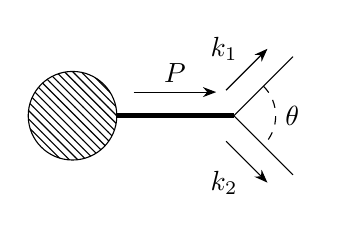
\begin{tikzpicture}
        \begin{feynman}
            % vertices
            \vertex (cen) at (0,0);
            \vertex (P) at (1.5,0.0);
            \vertex (k1) at (2.25,0.75);
            \vertex (k2) at (2.25,-0.75);
            \vertex (k1c) at (1.875,0.375);
            \vertex (k2c) at (1.875,-0.375);
            % edge labels
            % \vertex [left=3.0ptof l] (tl) {$a, \varepsilon_P$};
            % \vertex [above right=0.0pt and 3.0ptof u] (tu) {$b, \varepsilon_1$};
            % \vertex [below right=0.0pt and 3.0pt of r] (tr) {$c,\varepsilon_2$};
            % diagram
            \diagram* {
                (cen)
                -- [momentum=\(P\)]
                (P),
                (cen)
                -- [line width=1.8pt]
                (P),
                (P)
                -- [momentum=\(k_1\)]
                (k1),
                (P)
                -- [momentum'=\(k_2\)]
                (k2),
                (k1c)
                -- [dashed, quarter left, edge label=\(\theta\)]
                (k2c)
            };
            \node[blob, scale=1.5] at (-0.55,0) {};
        \end{feynman}
    \end{tikzpicture}
    \end{center}
    The virtuality of \(\ell\) is
    \begin{align}
        P^2
        =
        k_1^2 + k_2^2 + 2 k_1 \cdot k_2
        =
        2 E_1 E_2 \le(1 - \cos\theta\ri)
        \approx
        E_P^2 z(1-z) \theta^2
        \,.
    \end{align}


    Now we turn to a splitting process in which \(\ell\) is the result of an even earlier splitting.
    %
    The momenta of the parent of \(\ell\) is denoted \(Q\), and the momentum of its sibling is denoted \(P'\):
    \begin{center}
    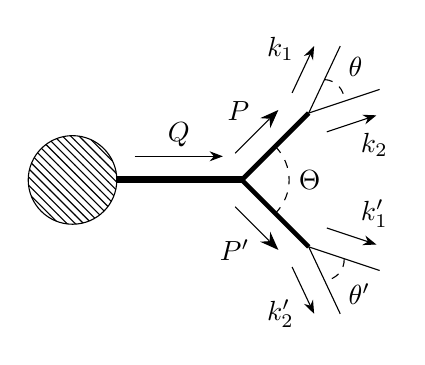
\begin{tikzpicture}
        \begin{feynman}
            % vertices
            \vertex (cen) at (0,0);
            \vertex (Q) at (1.6,0.0);
            \vertex (P) at (2.45,0.85);
            \vertex (Pp) at (2.45,-0.85);
            \vertex (k1) at (2.85,1.7);
            \vertex (k2) at (3.35,1.15);
            \vertex (k1p) at (3.35,-1.15);
            \vertex (k2p) at (2.85,-1.7);
            % centers, for angles
            \vertex (Pc) at (2.025,0.425);
            \vertex (Ppc) at (2.025,-0.425);
            \vertex (k1c) at (2.65,1.275);
            \vertex (k2c) at (2.9,1.0);
            \vertex (k1pc) at (2.9,-1.0);
            \vertex (k2pc) at (2.65,-1.275);
            % edge labels
            % \vertex [left=3.0ptof l] (tl) {$a, \varepsilon_P$};
            % \vertex [above right=0.0pt and 3.0ptof u] (tu) {$b, \varepsilon_1$};
            % \vertex [below right=0.0pt and 3.0pt of r] (tr) {$c,\varepsilon_2$};
            % diagram
            \diagram* {
                (cen)
                -- [line width=2.5pt]
                (Q),
                (cen)
                -- [momentum=\(Q\), opacity=0]
                (Q),
                (Q) [scale=2]
                -- [momentum=\(P\), line width=1.7pt]
                (P),
                (Q) [scale=2]
                -- [momentum'=\(P'\), line width=1.7pt]
                (Pp),
                (P)
                -- [momentum=\(k_1\)]
                (k1),
                (P)
                -- [momentum'=\(k_2\)]
                (k2),
                (Pp)
                -- [momentum=\(k_1'\)]
                (k1p),
                (Pp)
                -- [momentum'=\(k_2'\)]
                (k2p),
                % angles
                (k1c)
                -- [dashed, quarter left, edge label=\(\theta\)]
                (k2c),
                (k1pc)
                -- [dashed, quarter left, edge label=\(\theta'\)]
                (k2pc),
                (Pc)
                -- [dashed, quarter left, edge label=\(\Theta\)]
                (Ppc),
            };
            \node[blob, scale=1.5] at (-0.55,0) {};
        \end{feynman}
    \end{tikzpicture}
    \end{center}
    The virtuality of the parent of \(\ell\), with momentum \(Q\), is
    \begin{align}
        Q^2
        &=
        P^2 + P^{\prime\,2} + 2 P \cdot P'
        \\
        &=
        E_P^2 z(1-z) \theta^2
        +
        E_{P'}^2 z'(1-z') \theta^{\prime\, 2}
        +
        2 \le( E_P E_{P'} - \abs{\vec{P}}\abs{\vec{P}'}\cos\Theta\ri)
        \,.
    \end{align}

    Focusing now on the final terms, and using \(\abs{\vec{P}} / E_P = \sqrt{1 - P^2 / E_P^2} = 1 + z(1-z)\theta^2/2 + \mathcal{O}\le(\theta^4\ri)\) and similarly for \(P'\) we write
    \begin{align}
        2 \le(
            E_P E_{P'}
            -
            \abs{\vec{P}}\abs{\vec{P}'}\cos\Theta
        \ri)
        &=
        2 E_P E_{P'}\le(1 - \cos\Theta\ri)
        -
        2\abs{\vec{P}}\abs{\vec{P}'}
        \cos\Theta
        \,
        \le(1 - \frac{\vec{P}}{E_P} \frac{\vec{P'}}{E_{P'}}\ri)
        \\
        &\approx
        E_P E_{P'} \le(
            \Theta^2
            -
            z(1-z)\theta^2
            -
            z'(1-z')\theta^{\prime\,2}
        \ri)
        \,.
    \end{align}
    up to terms of \(\mathcal{O}(\Theta^4, \Theta^2 \theta^2, \theta^4)\), if we consider \(\theta\) and \(\theta'\) to be of the same order.

    Therefore, in the collinear limit for \(\Theta\), and defining \(Z = E_P / E_Q\) for continuity, we have
    \begin{align}
        \label{eq:mass-strong-ordering}
        Q^2
        =
        E_Q^2
        \,
        Z \le(1-Z\ri) \Theta^2
        \le(
            1 + \mathcal{O}\le(\theta^2/\Theta^2\ri)
        \ri)
        \,.
    \end{align}

    In \Eq{mass-strong-ordering}, we discard terms of higher order in both \(\Theta\) and \(\theta\), to highlight the crucial correction of \(\mathcal{O}(\theta^2/\Theta^2)\).
    %
    If we only assumed the collinear limit for \(\theta\) and \(\Theta\) independently, with no thought for the way they compare, then this term would have no reason to be small.
    %
    In particular, if we were worried about regions of phase space for which \(\theta\) and \(\Theta\) are similar, then we might feel quite daunted by this result.

    Luckily, we are \textit{not} worried about terms of \(\mathcal{O}(\theta/\Theta)\).
    %
    We are saved by the principle of strong angular ordering%
    \footnote{
        That is, as long as we work in the collinear limit with no thought for detailed azimuthal correlations.
    }
    %
    In particular, strong angular ordering gives us \Lem{cascade-angular-ordering}, implying that \(\theta^2 / \Theta^2 \ll 1\).
    %
    In the limit of strong angular ordering, the phase space for a soft gluon emitted at the angle \(\theta\) is \textit{completely dominated} by the region in which \(\theta\) is much smaller than any other -- \(\Theta\) included.

    Therefore, \(Q^2 = E_Q^2 Z(1-Z)\) up to terms which are erased by our approximations and assumptions, and we may continue recursively factorizing the cross section treating \(\ell^*\) and \(\ell^{'\,*}\) as on shell.
\end{example}

\textbf{By dropping terms of \(\mathcal{O}(\theta^2/\Theta^2)\) -- justified by strong angular ordering and \Lem{cascade-angular-ordering}-- we may recursively apply the principles of the previous chapter}, including collinear phase space, splitting functions, and angular ordering.
%
In this way, we can obtain expressions for differential cross sections involving an arbitrary number of external particles in the limit in which they are all collinear.%
\footnote{
    As usual, for observables which are insensitive to detailed azimuthal information.
}
We have a model of the detailed inner structure of jets.



\begin{exercise}
    \label{ex:all-on-shell-proof}
    Show that the details of \Example{everything-on-shell} do not change even when \(k_1\) and \(k_2\) are themselves intermediate lines, so that the arguments of \Example{everything-on-shell} is sufficient to prove \Prop{everything-on-shell}.%
    \footnote{
        A good thing we could stop there, too.
        %
        I was running out of symbols!
    }
\end{exercise}

\remark{}{
    The cascade model for jet formation that we have derived in this section is simple and powerful;
    %
    it reproduces the behavior of \gls{qcd} differential cross sections in their most singular regions -- the \glslink{soft-limit}{soft} and \glslink{collinear-limit}{collinear} regions of phase space.
    %
    A more detailed discussion verifies that our description indeed captures the most singular features of scattering involving \gls{qcd} partons (see e.g. \Reff{Marchesini:1994wr} and citations therein).
    %
    However, since the partonic cascade model derived above misses several important features of \gls{qcd} anyway, we will not spend more time discussing its formal features;
    %
    notably, parton showers valid in the strong-ordering regime give incorrect estimates for a variety of important effects and distributions, ranging from the conceptually simple physics of the transverse momentum distribution of hadrons in Drell--Yan processes to the complicated physics of color correlations \cite{Collins:2011zzd,Dasgupta:2018nvj,Hamilton:2020rcu}.
}


The model of the partonic cascade we have found above allows us to recursively calculate features of \(N\)-particle differential cross sections:
%
the probability to produce \(N\) particles is related to the probability to produce \(N-1\), and so on.
%
Framing our results in a probabilistic fashion paves the way to another idea, however:
%
we may use our insights to algorithmically \textit{produce} \(N\) particle configurations, given a configuration of some number \(N-M\) of original particles.
%
If we compute the differential cross section for a process with two outgoing, final-state particles, we can use our results to obtain the differential cross section with \textit{any} number of final states.
%
We split two particles into three, then three into four, and so on, holding always to the tenets of angular ordering and using the probability distribution
\begin{align}
    \label{eq:splitting-prob-ch3}
    \dsigmatilde_{ij \leftarrow \ell^*}
    =
    \frac{\alphas}{2\pi}
    P_{ij \leftarrow \ell}(z_i) \frac{\dd z_i \dd s}{s}
    =
    \frac{\alphas}{\pi}
    P_{ij \leftarrow \ell}(z_i) \frac{\dd z_i \, \dd \theta}{\theta}
    \,,
\end{align}
as in \Eq{dsigmatilde_definition} of \Sec{splitting-functions}, for each splitting.
%
This procedure allows us to simulate the energy flow of a particle collision event not in the formal language of quantum field theory, but as a \textbf{classical, Markovian branching process}.
%
Simulations of this nature -- called \vocab{parton showers} -- are employed in more complicated forms as some of the most important tools of particle physics.

\remark{}{
    We also need to know the probability that \emph{no} splitting occurs, however.
    %
    To explore this further, see \Prob{no-emission}.
}

\begin{definitionbox}{Parton Shower}{parton-shower}
    A \glslink{partonshower}{\vocab{parton shower}} is any probabilistic algorithm that applies the principles of the partonic cascade to produce final-state particles given an initial set of particles:
    %
    the initial set of particles are split recursively using splitting probabilities governed by splitting functions, until a stopping condition is reached.
    %
    The tree formed by the recursive splitting of initial-state partons is called the \vocab{jet tree};
    %
    see \Fig{jet-tree}.

    The set of initial particles serving as an input to the shower is often a low-multiplicity set of particles emerging from a hard process, as determined by an explicit matrix element calculation.
\end{definitionbox}


\begin{figure}[]
    \centering
    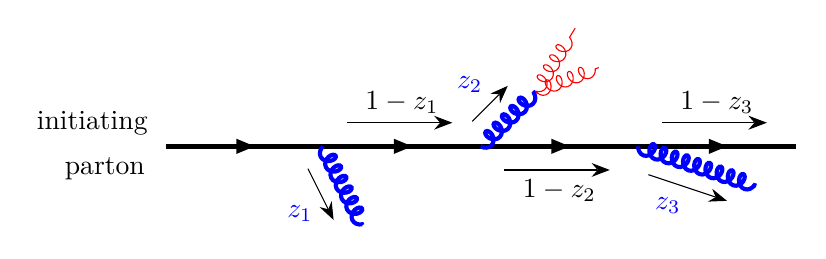
\begin{tikzpicture}
        \begin{feynman}
            % vertices
            \vertex (i) at (-4,0);
            \vertex (split1) at (-2,0.0);
            \vertex (split2) at (0,0.0);
            \vertex (split3) at (2,0.0);
            \vertex (p1) at (-1.5, -1.0);
            \vertex (split22) at (0.7,0.7);
            \vertex (p21) at (1.2, 1.5);
            \vertex (p22) at (1.5, 1.0);
            \vertex (p3) at (3.5, -0.5);
            \vertex (f) at (4,0);
            % edge labels
            \vertex [above left=0.5pt and 3.0pt of i] (labeli) {initiating};
            \vertex [below left=0.5pt and 4.0pt of i] (labeli) {parton};
            % \vertex [above right=0.0pt and 3.0ptof u] (tu) {$b, \varepsilon_1$};
            % \vertex [below right=0.0pt and 3.0pt of r] (tr) {$c,\varepsilon_2$};
            \diagram* {
                (i) -- [fermion, line width=1.6pt] (split1),
                (split1) -- [fermion, line width=1.6pt, momentum={\(1-z_1\)}] (split2),
                (split2) -- [fermion, line width=1.6pt, momentum'={\(1-z_2\)}] (split3),
                (split3) -- [fermion, line width=1.7pt, momentum={\(1-z_3\)}] (f),
                (split1) -- [gluon, blue, line width=1.5pt, momentum'={\(z_1\)}] (p1),
                (split2) -- [gluon, blue, line width=1.5pt, momentum={\(z_2\)}] (split22),
                (split22) -- [gluon, red] (p21),
                (split22) -- [gluon, red] (p22),
                (split3) -- [gluon, blue, line width=1.5pt, momentum'={\(z_3\)}] (p3),
            };
        \end{feynman}
    \end{tikzpicture}
    \caption[A visualization of a jet tree formed by recursively splitting an initiating parton.]{
    A visualization of a jet tree (\textit{not} a Feynman diagram) formed by recursively splitting an initiating parton.
    %
    The label \(z_i\) or \(1-z_i\) at each splitting labels the energy fraction of each child of a splitting relative to its parent.
    %
    The black fermion line indicates the \textit{hard branch} of the jet tree, while the blue gluon lines indicate \textit{primary} branches of the jet tree.
    }
    \label{fig:jet-tree}
\end{figure}

The \textit{initiating Parton} and \textit{hard/primary branchings} will be important for the computations of the rest of the chapter:
\begin{definitionbox}{Initiating parton}{}
    The \vocab{initiating parton} of a jet tree is an input particle to a parton shower algorithm which is then recursively split.
\end{definitionbox}

\begin{definitionbox}{Hard and Primary Branches}{}
    The \vocab{hard branch} of a jet tree is the path formed by recursively following the hardest parton at every splitting of the initiating parton.
    %
    It is visualized as a black fermion line in \Fig{jet-tree}.

    The \vocab{primary branches} of a jet tree are the softer branchess of the splittings from the hard branch of the jet tree.
    %
    They are visualized as blue gluon lines in \Fig{jet-tree}.
\end{definitionbox}

Explicitly constructing a simple parton shower is the business of \Probs{veto-algorithm}{parton-shower}.
%
Now, let us explore the implications of our model.


% ---------------------------------------
\subsection{Substructure Diagrams and Additive Observables}
% ---------------------------------------
\label{sec:ll-substructure-diagrams}

We will begin our quantitative discussion of the partonic cascade by characterizing its properties with particularly simple observables.
%
In particular, we will discuss \emph{\glspl{additive-observable}}, which leverage the recursive structure of the partonic cascade:%
\footnote{
    Additivity is a simple, sufficient condition which guarantees the validity of the resummation of \glspl{substructure-diagram} discussed here.
    %
    However, the requirement of additivity can be weakened without changing the conclusions of this section;
    %
    a weaker but still sufficient condition, named \textit{recursive infra-red and collinear (rIRC) safety}, was introduced by \Reff{Banfi:2004yd}.
    %
    The definition of rIRC safety is given in Eqs.\ (3.4) and (3.5) of \Reff{Banfi:2004yd}, and an example of additivity is furnished by the thrust observable, discussed in Section 3.2 of \Reff{Banfi:2004yd}.
}

\begin{definitionbox}{Additive Observable}{additive-observable}
    For the purposes of this thesis, an \vocab{\gls{additive-observable}} is a collider observable which can be written as a sum over positive, monotonic contributions from final state particles, such that the contribution of any final state particle vanishes if the energy fraction \(z_i\) vanishes or if the angle \(\theta_i\) relative to the jet vanishes:
    \begin{align}
        X(p_1,\,\cdots,\,p_n)
        &=
        \sum_{i=1}^n X(p_i)
        =
        \sum_{i=1}^n X(z_i, \theta_i)
        \,,
    \end{align}
    with \(X(z, \theta)\) monotonic in both \(z\) and \(\theta\), and
    \begin{align}
        \lim_{z \to 0} X(z, \theta)
        =
        \lim_{\theta \to 0} X(z, \theta)
        =
        0
        \,,
    \end{align}
    and we have again abused notation to denote that the value of \(X\) evaluated on a single particle depends on the energy fraction and angle of the particle relative to the jet.
\end{definitionbox}

    Angularity, \(e_\varsigma = \sum_i z_i \theta_i^\varsigma\), is an additive observable.
    %
    Observables such as the jet mass and jet GECFs can be approximated as additive observables at \glslink{accuracy}{LL} because of the presence of soft and collinear singularities.
    %
    In particular, the singular nature of the splitting probabilities of \Eq{splitting-prob-ch3} in the limits \(z,\,\theta \to 0\) indicates that the phase space of partonic emissions is dominated by emissions with small energy fraction \(z\) and angle \(\theta\), so that \(z(1-z) \approx z\).%
    %
    The problems posed by these singularities are addressed systematically by resummation, and we exposit a simple resummation method in this section.


Additive or approximately additive observables can therefore be approximated as sums of contributions from \emph{primary branches within the jet tree} in the limit of strong angular ordering.
%
For example, the angularity \(e_\varsigma\) takes the approximate form
\begin{align}
    e_\varsigma
    =
    \sum_{\text{particles } i}
        z_i \theta_i^\varsigma
    \quad
    \approx
    \sum_{\substack{\text{primary}\\\text{branches } i}}
        z_i \theta_i^\varsigma
    \,,
\end{align}
due to the soft and collinear enhancement of the phase space of these emissions.
%
It is for this reason that additive observables leverage and can illuminate the validity of the partonic cascade of pQCD.

\begin{exercise}
    Prove the claim above by using momentum conservation and strong angular ordering of the splittings of primary branches.
\end{exercise}



\begin{example}
    \label{ex:dyson-substructure}
    Consider the additive observable \(X\) that can be expressed (abusing notation) as
    \begin{align}
        X(\text{jet})
        =
        \sum_{\substack{\text{primary}\\\text{branches } i}}
        X(z_i, \theta_i)
        \,.
    \end{align}
    %
    We now design a formula for the cumulative probability distribution of \(X\) when it is computed on jets formed by an initiated parton of flavor \(i\).

    Using the principles of strong angular ordering and the soft limit, we can write its cumulative probability distribution in the partonic cascade model as
    \begin{align}
        \label{eq:general-additive-cumulative-distribution}
        \Sigma_X(x)
        &=
        \delta(x)
        \\
        \notag
        &\quad
        +
        \sum_{i = n}^\infty
        \,\,
        \le(
        \int_0^R \frac{\dd\theta_1}{\theta_1}
        \int_0^1 \dd z_1
        \frac{\alphas}{\pi}
        p_i(z_1)
        \ri)
        \le(
        \int_0^{\theta_1} \frac{\dd\theta_2}{\theta_2}
        \int_0^1 \dd z_2
        \frac{\alphas}{\pi}
        p_i(z_2)
        \ri)
        \cdots
        \\
        &\qquad\qquad\qquad\qquad
        \Theta(x > \sum_{k = 1}^n X(z_k, \theta_k))
        \,,
    \end{align}
    where the delta function emerges because we assume \(X = 0\) when evaluated on a single particle, and the bounds of integration on the angular integrals are a result of strong angular ordering.
    %
    We may use \(p_i(z) \approx 2 C_{R_i} / z\) -- the soft limit for the emission of a gluon from the initiating parton -- for each emission, because the emission of a soft gluon of momentum fraction \(z\) does not change the flavor of a parton:
    %
    a quark emitting a gluon remains a quark, and similarly a gluon remains a gluon after the soft emission.

    Now we can use \textit{Dyson's trick} to further simplify this integral.
    %
    Noting that no piece of the integrand actually depends on the \textit{ordering} of the \(\{\theta_n\}\), we can make the replacement
    \begin{align}
        \int_0^R \frac{\dd\theta_1}{\theta_1}
        \int_0^{\theta_1} \frac{\dd\theta_2}{\theta_2}
        \int_0^{\theta_2} \frac{\dd\theta_3}{\theta_3}
        \cdots
        \int_0^{\theta_{n-1}} \frac{\dd\theta_n}{\theta_n}
        =
        \frac{1}{n!}
        \int_0^R \frac{\dd\theta_1}{\theta_1}
        \int_0^R \frac{\dd\theta_2}{\theta_2}
        \cdots
        \int_0^R \frac{\dd\theta_n}{\theta_n}
        \,,
    \end{align}
    without changing the value of the integral in \Eq{general-additive-cumulative-distribution}.

    Therefore, we can write
    \begin{align}
        \label{eq:dysons-additive-cumulative-distribution}
        \Sigma_X(x)
        &=
        \delta(x)
        \,\,
        +
        \,\,
        \sum_{i = n}^\infty
        \frac{1}{n!}
        \,\,
        \prod_{k = 1}^n
        \le(
        \int_0^R \frac{\dd\theta_k}{\theta_k}
        \int_0^1 \dd z_k
        \frac{\alphas}{\pi}
        p_i(z_1)
        \ri)
        \,\,
        \Theta\le(x > \sum_{k = 1}^n X(z_k, \theta_k)\ri)
        \,,
    \end{align}
    providing us with an extremely compact form for the cumulative distributions of additive observables.

    However, we can do even better.
    %
    The sum on \(n\) and \(1/n!\) already hint at a wonderful feature:
    %
    \textbf{the cumulative distributions of additive observables \textit{exponentiate} in the soft-collinear limit}.
\end{example}

\begin{exercise}
    By using the plus-function regulated form of the splitting functions -- and in particular that \(p_i(z) \approx 2 C_{R_i} \le[1 / x\ri]_+\) in the soft limit -- show that \Eq{dysons-additive-cumulative-distribution} corresponds to a properly normalized probability distribution.
\end{exercise}


\begin{proposition}{LL Distributions for Additive Observables}{ll-additive}
    We may describe the \glslink{accuracy}{LL} cumulative probability distribution \(\Sigma^{\rm(LL)}_X(x)\) of an additive observable \(X\) as the probability that \textit{no emission} contributes a value greater than \(x\) to \(X\), up to sub-leading behavior in \(\alphas\) and logarithms or powers of the observable.
    \begin{align}
        \label{eq:ll-additive}
        \Sigma^{\text{(LL)}}_X(x) \approx \mathbb{P}(X_i < x \text{ for all } i)
        \,.
    \end{align}

    It is the right-hand side of the equation above that we will be able to address simply with \glspl{substructure-diagram}.
\end{proposition}


\begin{proof}

First, we recall that the \emph{\gls{vetoreg}} for a collider observable \(X\) and a value \(x\) is a region of the \((z, \theta)\) phase space for which \(X(z,\theta) > x\).
%
Since we have defined additive observables to be the sum of \textit{positive} contributions, this means that if any partonic emission lies in the veto region, then \(X > x\).
%
Therefore, when calculating the cumulative probability distribution for the observable \(X\), \(\Sigma_X(x)\), additive observables cannot lie in the veto region.

The calculation of distributions for additive observable is dramatically simplified at \glslink{accuracy}{LL}, where the assumption of angular ordering holds, by the soft and collinear singularities of pQCD.
%
The strong angular ordering of \Sec{everything-on-shell} implies that the primary branches of a jet satisfy \(\theta_1 \gg \theta_2 \gg \cdots \gg \theta_n\), so that additive observables \(X\) tend to be dominated by the contribution of a single emission -- generally the widest emission -- whose contribution to \(X\) is exponentially higher than the values contributed by other branches of the partonic cascade.

In more mathematical language, let us consider an additive observable with contributions \(X(z_i, \theta_i) = X_i > 0\) from emissions \(i\).
%
At \glslink{accuracy}{LL}, we have asserted that there is a dominant contribution \(X = \max_i x_i\) such that \(X = \sum_i X_i \approx \max_i X_i\).
%
We may therefore approximate the cumulative probability distribution for \(X\), \(\Sigma_X(x) := \mathbb{P}(X = \sum_i X_i < x)\), by the probability that the value of \(X_i\) for any emission is less than the dominant value, which in turn is less than \(x\):%
\footnote{
    More generally, we can write \textit{without approximation} that \(\Theta(x - \sum_i X_i) \leq \prod_i \Theta(x - X_i)\), where equality emerges when we have at most a single non-zero \(x_j = X\).
    %
    Using that the cumulative distribution for \(X\) is the expectation value of the left-hand side, we may take the expectation value of both sides to obtain \(\Sigma_X(x) \leq \mathbb{P}(X_i < x \text{ for all } i)\), which provides a helpful upper bound for the full cumulative distribution of an additive observable.
}
\begin{align}
    \Sigma_X(x) \approx \mathbb{P}(X_i < x \text{ for all } i)
    \,.
\end{align}
%
This approximation holds up to corrections due to multiple emissions, which we address in \Prob{multiple-emissions}, that are sub-leading in \(\alphas\) and logarithms of the observable.
%
We should also note that typically, calculations applying the \glslink{accuracy}{LL} approximation will also drop terms that are suppressed by powers of \(X\) since these are sub-dominant to the leading logarithmic terms in observable distributions.
\end{proof}



\remark{}{
    An incredible resource for learning more about the calculation of observables in the framework of this section, and of groomed observables discussed in the following chapter, is the book \emph{Looking inside jets: an introduction to jet substructure and boosted-object phenomenology} \cite{Marzani:2019hun}, whose pedagogy, detail, and beautiful exposition we are unable to match.
    %
    Interested or confused readers should consult their treatment as well.
}

\begin{example}
The approximate mass of a jet due to a single emission is given by \(m^2 = Q^2 z\theta^2\), where \(Q\) is the total energy of the jet.
%
Therefore, mass is an approximately additive observable.

Using \Example{dyson-substructure} and \Prop{ll-additive}, and using the reduced splitting functions of \Sec{fixed-order-substructure}, the jet mass distribution is given at LL by
%
\begin{equation}
\label{eq:LL_mass}
\begin{aligned}
    \Sigma^{\rm(LL)}_{m^2}(m^2)
    &=
    \sum_{n = 0}^{\infty}\frac{1}{n!}
    \left(
    \frac{\alphas}{\pi}
    \int_0^R \frac{\dd\theta}{\theta}
    \int_0^{\frac{1}{2}} \dd z\,[\bar{p}_i(z)]_+^{[1/2]}
    \Theta\left(
    \frac{m^2}{Q^2} - z\theta^2
    \right)
    \right)^n
    \\
    &=
    \exp\left[
    -\frac{\alphas}{\pi}
    \int_0^R \frac{\dd\theta}{\theta}
    \int_0^{\frac{1}{2}} \dd z\,\bar{p}_i(z)
    \Theta\left(
    z \theta^2 - \frac{m^2}{Q^2}
    \right)
    \right]
    .
\end{aligned}
\end{equation}


Let us pursue this derivation graphically by using \glspl{substructure-diagram}.
%
By following the integral expressions of \Eq{LL_mass}, the LL cumulative distribution for the mass-squared of a jet is
\begin{equation}
\begin{aligned}
    \Sigma^{\rm(LL)}_{m^2}(m^2)
    &=
    \sum_{n = 0}^{\infty}\frac{1}{n!}
    \left(
    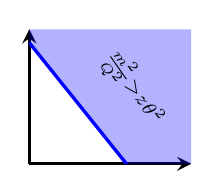
\begin{tikzpicture}[
    baseline={([yshift=-.8ex]current bounding box.center)},
    vertex/.style={anchor=base,
    circle,fill=black!25,minimum size=18pt,inner sep=2pt},
    scale=.3]
    \begin{axis}
    [xmin=0, xmax=5,
    ymin=0, ymax=5,
    axis line style = very thick,
    axis y line*=left,
    axis x line*=bottom,
    axis lines = middle,
    ticks=none]
    	\addplot[name path=f, domain=0:5,
        style=very thick, blue]
        {4.5-1.5*x};
        \path[name path=axis]
        (axis cs:0,5) -- (axis cs:5,5);
        \addplot [
            thick,
            color=blue,
            fill=blue,
            fill opacity=0.3
        ]
        fill between[
            of=f and axis
        ];
        \node [rotate=-55] at (axis cs:  3.2,  2.8)
        {${\scriptstyle \frac{m^2}{Q^2} > z\theta^2}$};
    \end{axis}
    \end{tikzpicture}
    \right)^n
    =
    \exp\left[
    ~-~
    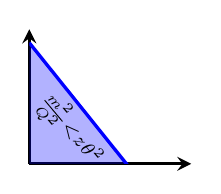
\begin{tikzpicture}[
    baseline={([yshift=-.8ex]current bounding box.center)},
    vertex/.style={anchor=base,
    circle,fill=black!25,minimum size=18pt,inner sep=2pt},
    scale=.3]
    \begin{axis}
    [xmin=0, xmax=5,
    ymin=0, ymax=5,
    axis line style = very thick,
    axis y line*=left,
    axis x line*=bottom,
    axis lines = middle,
    ticks=none]
    	\addplot[name path=f, domain=0:5,
        style=very thick, blue]
        {4.5-1.5*x};
        \path[name path=axis]
        (axis cs:0,0) -- (axis cs:1,0);
        \addplot [
            thick,
            color=blue,
            fill=blue,
            fill opacity=0.3
        ]
        fill between[
            of=f and axis
        ];
        \node [rotate=-50] at (axis cs:  1.25,  1.25)
        {${\scriptstyle \frac{m^2}{Q^2} < z\theta^2}$};
    \end{axis}
    \end{tikzpicture}
    ~~
    \right]
    %\approx
    %\exp\left[~-\frac{C_R\alphas}{2 %\pi}\log^2\left(\frac{m^2}{Q^2}\right)\right]
    ,
\end{aligned}
\end{equation}
where the first equality gives the probability that no emission in the jet is associated with an approximate mass-squared \(z\theta^2\) larger than \(m^2\) -- the argument of the cumulative distribution -- and the second equality follows from using the fact that \glspl{plus-fn} integrate to zero (see the diagrammatic identity of \Eq{plus-fn-diagram-identities}).
%
In the final equality, we see that the LL cumulative distribution is one over the exponent of the \gls{radiator} (the area of the \gls{vetoreg}).

Plugging in the important piece for the splitting function at leading logarithmic accuracy (i.e. in the soft limit), \(p(z) \approx 2 C_R / z\) for a jet formed by particles with \(SU(3)\) color representation \(R\), and putting back in factors of \(Q\), we find
\begin{align}
    \label{eq:mass-ll-cumulative}
    \Sigma^{\rm(LL)}_{m^2}(m^2)
    =
    \exp\left[~-\frac{C_R\alphas}{2 \pi}\log^2\left(\frac{m^2}{Q^2}\right)\right]
    \,,
\end{align}
%
with an associated probability distribution
\begin{align}
    \rho^{\rm(LL)}_{m^2}(m^2)
    =
    \frac{C_R \alphas}{\pi}
    \frac{1}{m^2}
    \log\le(\frac{Q^2}{m^2}\ri)
    \,
    \exp\left[~-\frac{C_R\alphas}{2 \pi}\log^2\left(\frac{m^2}{Q^2}\right)\right]
    \,.
\end{align}

Notably, the cumulative distribution of \Eq{mass-ll-cumulative} is the exponential of the radiator that appeared in \Example{mass-fixed-order}.
\end{example}


\remark{}{
    We emphasize again that by focusing on the singular pieces of the splitting function, we implicitly focus on the probability that a \emph{gluon} is emitted from the parent parton.
    %
    For example, a quark may emit a gluon, so that the resulting final state consists of both a gluon and a quark, while a gluon may split into two gluons.
    %
    In the language of splitting functions, a gluon may in principle split into two quarks;
    %
    however, the associated splitting function does not have any singularities as \(z \to 0\) and is therefore sub-leading to the singular behavior reflected by the approximation \(p(z) \approx 2 C_{R} / z\).
}



%\begin{exercise}
%    When expanded to \(\mathcal{O}(\alphas)\), there is a small discrepancy between the LL result for the cumulative mass-squared distribution above and the NLO result presented in \Sec{fixed-order-substructure}.

%    What is the source of this discrepancy?
%    %
%    Argue that it has no effect away from \(m^2 = 0\), and gives a contribution at \(m^2 = 0\) is associated with the probability of no splittings occurring in the jet.
%\end{exercise}


\begin{exercise}
    \label{ex:ll-angularity-radiator}
    The slopes of the diagonal line in the substructure diagram in the calculation of the jet mass distribution are \(-2\) since, for constant \(m^2\), \(z \sim 1/\theta^2\) and \(\log(1/z) = \text{const} - 2 \log(1/\theta)\).
    %
    What are the slopes of the diagonal lines involved in the computation of jet \glspl{angularity}?

    Represent the LL distribution of jet angularities with a \gls{substructure-diagram}, and show that it takes the approximate analytic form
    \begin{align}
        \Sigma^{(\text{LL})}(e_\varsigma)
        \approx
        \exp\le[
            -\frac{C_R\alphas}{\varsigma \pi}\log^2(e_\varsigma)
        \ri]
        \,,
    \end{align}
    in the soft limit.
\end{exercise}

We can improve the accuracy of the results obtained above with our \glspl{substructure-diagram} with two simple tricks:
%
adding running coupling effects, and adding effects from multiple emissions.
%
Calculations accounting for effects from the running of the QCD coupling and multiple emissions within a jet are called \glslink{accuracy}{modified leading logarithmic (MLL)} calculations.

MLL calculations of additive jet substructure observables capture nearly all of the effects of a \glslink{accuracy}{next-to-leading logarithmic (NLL)} calculation \cite{Marzani:2019hun}.
%
Missing, however, are \vocab{non-global logarithms} -- contributions to jet substructure from partonic radiation in which a branch of the partonic tree of emissions occurs at a wider angle than would be captured by the jet, but one of whose children re-enters the jet cone.\cite{Dasgupta:2001sh,Appleby:2002ke,Weigert:2003mm,Rubin:2010fc,Banfi:2010pa,Hornig:2011iu,Kelley:2011aa,Hatta:2013iba,Schwartz:2014wha,Khelifa-Kerfa:2015mma,Larkoski:2016zzc,Marzani:2019hun,Banfi:2021owj,Banfi:2021xzn}

Luckily, because the radiation which contributes to non-global logarithms arises from radiation which was at first outside of the jet, it is associated with \textit{wide angles}, and wide angle radiation tends to be low-energy (see, e.g. \Reff{Larkoski:2014wba} and references therein).

Therefore, if we can find a way to exclude low-energy radiation from the interior of a jet, there is some hope that we may avoid non-global logarithms altogether, such that running coupling effects together with multiple emissions are sufficient to provide NLL results!
%
Indeed, this will occur when applying certain techniques of \gls{jet-grooming} for removing soft radiation from jets, such as \textit{Soft Drop with \(\beta_\text{sd}= 0\)}, which we explore in the next chapter.


\remark{}{
    To include running coupling effects and work towards an MLL description of additive jet observables, we notice that the splittings of perturbative QCD should be governed by an \textit{effective coupling} \(\alphas(\kappa)\), where \(\kappa = \kappa(z,\theta)\) is a scale associated with the splitting.
    %
    The result would involve integrals containing terms of the form \(\int \dd z \, \dd \theta \, \alphas(\kappa) \, p(z) / \theta\).
    %
    The precise value we should choose for \(\kappa\) in order to account for higher-order effects is not obvious, but \Reff{Amati:1980ch} showed that \(\kappa\) should be given by the transverse momentum of the splitting in order to minimize the effects of large logarithms in perturbative calculations:
    \begin{align}
        \kappa \approx Q z(1-z)\sin\theta \approx Q z \theta
        \,.
    \end{align}
    %
    In particular, QCD correlations and cross sections that use \(\alphas\) evaluated at a scale \(\kappa\) generically include logarithms of the form \(\log(p_{\perp} / \kappa)\).
    %
    To make these logarithms small, one may choose \(\kappa \sim p_\perp\), which then requires that we evaluate the strong coupling at the scale \(p_\perp\) as well.
    %
    This prescription provides a straightforward procedure for understanding higher-order effects with \glspl{substructure-diagram}, and can be extended to higher perturbative accuracy with the Catani-Marchesini-Webber (CMW) prescription \cite{Catani:1990rr}, which achieves two-loop accuracy for the running of \(\alphas\), and to qualitatively include non-perturbative effects by \textit{freezing} the coupling, as discussed in \App{soft-distortions}.
    %
    As a reminder, the one-loop running of \(\alphas\) is captured by
    \begin{align}
        \alpha^{\rm 1-loop}_s(\kappa)
        =
        \frac{\alphas(Q)}{1 + \alphas(Q) \beta_0 \log(\frac{\kappa}{Q})/2\pi}
        ,
    \end{align}
    where \(\beta_0 = \frac{11}{3}C_A - \frac{4}{3} T_f n_f\) is a coefficient appearing in the QCD beta function: \(\beta(\alphas) = -\beta_0 \alphas^2/2\pi + \mathcal{O}(\alphas^3)\).
}


To include more detail about the effects of multiple emissions, and achieve a full MLL description of additive jet obervables, we will need to use the full expression \(X = \sum_i X_i\) rather than the LL approximation \(X \approx \max_i X_i\) used above.
%
Concretely, this means that the effects of multiple emissions for an additive observable can be computed via the infinite-product integral
\begin{align}
    \label{eq:series-multiple-emissions}
    \Sigma_X(x)
    &=
    \sum_{n = 0}^{\infty}
    \frac{1}{n!}
    \prod_{k = 1}^n
    \left(
        \int_0^R \frac{\dd\theta_k}{\theta_k}
        \int_0^{\frac{1}{2}} \dd z_k
        \,\,
        \frac{\alphas}{\pi}
        \,\,
        [\bar{p}_i(z_k)]_+^{[1/2]}
    \right)^n
    \Theta\left(
        \frac{m^2}{Q^2} - \sum_k X(z_k, \theta_k)
    \right)
    \,.
\end{align}
%
At face value, this seems much more difficult to evaluate than the LL integral for the radiator of \(X\).
%
It is not at all obvious whether the contributions of multiple emissions exposed by \Eq{series-multiple-emissions} will even lead to an exponential form for the cumulative distribution of \(X\) --
indeed, \textit{they don't}.

It may seem miraculous, then, that a detailed analysis of \Eq{series-multiple-emissions} involving Laplace transforms shows that the effects of multiple emissions can \textit{still} be captured only with the radiator for \(X\) -- the integral over the veto region which appears in the \glslink{accuracy}{LL} results above.
%
In particular, the most important effects due to a more detailed analysis of multiple emission contributions to additive observables can be captured by the cumulative distribution
\begin{align}
    \label{eq:resummed-multiple-emissions}
    \Sigma_X(x)
    &=
    \frac{\exp\le(-R_X(x) - \gamma_E R'_X(x)\ri)}{\Gamma\le(1 + R'_X(x)\ri)}
    \,,
\end{align}
where \(\gamma_E=0.577\dots\) is the Euler-Mascheroni constant, \(\Gamma\) is the familiar Euler Gamma function, and \(R'_X(x) := -\dd R_X(x) / \dd \log(x)\).
%
The proof of this formula for the simple case of angularities, is the business of \Prob{multiple-emissions}.
%
In \Prob{multiple-emissions}, we also show that including the effects of multiple emissions leads to a cumulative distribution for \(X\) depending on the derivative of the radiator for general additive observables;
%
this feature will resurface in our discussion of continuity and jet grooming in \Chap{grooming}.



%\begin{exercise}
%    Argue that the total energy fraction of all particles in a jet with energy \(z < \zcut\) and \(\theta > \thetacrit\),
%    \begin{align}
%        \zpre
%        \quad
%        :=
%        \sum_{\substack{
%                \text{particles }i\text{ with}
%                \\
%                \theta_i > \thetacrit,
%                \,\,\,
%                z_i < \zcut
%        }} z_i
%    \end{align}
%    is an additive collider observable (albeit a discontinuous one), and that its cumulative distribution at LL is
%    % it is the sum of monotonic, positive contributions of different emissions which vanishes when either \(z_i\) vanishes or \(\theta_i\) vanishes.
%    %
%    % Therefore, it can be captured with \glspl{substructure-diagram}, and its cumulative distribution at LL is
%    \begin{equation}
%    \begin{aligned}
%        % \rho(z_{\rm pre}, \thetacrit)
%        % &=
%        % \left(\frac{2 C_R \alphas}{\pi}\right)^2
%        % \frac{1}{\theta}
%        % \log(\thetacrit)
%        % [p(z_{\rm pre})]_+
%        % \int_{z > z_{\rm pre}} z~\dd\log(z) [p(z)]_+
%        % \\
%        % &\ \ \ \ \ \ \ \ \ \ \
%        % \times
%        \Sigma(\zpre | \thetacrit)
%        &=
%        \exp\left[
%        ~-~
%        \begin{tikzpicture}
%        [baseline={([yshift=-.8ex]current bounding box.center)},
%        vertex/.style={anchor=base,
%        circle,fill=black!25,minimum size=18pt,inner sep=2pt},
%        scale=.3]
%        \begin{axis}
%        [xmin=0, xmax=5,
%        ymin=0, ymax=5,
%        axis line style = very thick,
%        axis y line*=left,
%        axis x line*=bottom,
%        axis lines = middle,
%        ticks=none]
%            \addplot[name path=f,domain=0:2.3,
%            style=very thick,blue]
%            {2.5};
%            \addplot[very thick, samples=50, smooth,domain=0:6,blue, name path=three] coordinates {(2.3,-1)(2.3,2.5)};
%            \path[name path=axis]
%            (axis cs:0,0) -- (axis cs:2.3,0);

%            \addplot[name path=pre,domain=0:2.3,
%                    style=very thick,magenta]
%                    {2.6};
%            \addplot[name path=pre2,domain=0:2.3,
%                    style=very thick,magenta]
%                    {4.};
%            \addplot[very thick, samples=50, smooth,domain=0:6,magenta, name path=three] coordinates {(2.3,2.525)(2.3,4)};
%            \path[name path=axispre]
%            (axis cs:0,4) -- (axis cs:2.3,4);
%            \addplot [
%                thick,
%                color=blue,
%                fill=blue,
%                fill opacity=0.3
%            ]
%            fill between[
%                of=f and axis
%            ];
%            \addplot [
%                thick,
%                color=magenta,
%                fill=magenta,
%                fill opacity=0.3
%            ]
%            fill between[
%                of=pre and axispre
%            ];
%        \end{axis}
%        \end{tikzpicture}
%        ~~
%        \right]
%        \,,
%    \end{aligned}
%    \end{equation}
%    where the blue and pink colorations have no distinct meaning other than ease of comparison to the previous exercise:
%    %
%    the blue box and the pink box together combine to give the overall veto region for \(\zpre\).
%    %
%    The blue box indicates the portion of the veto region with \(\theta > \thetacrit\) and \(z > \zcut\), while the pink box indicates the portion with \(\theta > \thetacrit\) and \(\zcut > z > \zpre\).
%\end{exercise}



\remark{}{
    Conditional distributions of jet parameters can also be important tools in physical applications. In general, the best way to calculate conditional distributions is not to calculate a single Sudakov exponent associated with the related parameters. Instead, it is best to compute the Sudakov exponent associated with the joint cumulative probability of all the involved parameters, find the associated probability distributions, and then divide by the probability distributions you are taking as conditional:
    \begin{align}
        \rho(a | b, c, ...) = \frac{\rho(a, b, c, ...)}{\rho(b, c ...)}
        .
    \end{align}
    %
    Computations of conditional distributions can be important in analytic studies of jet grooming, and make an in the jet grooming calculations of \Chap{grooming}.
}


We have begun to utilize the fractal structure of jets to understand the behavior of jet substructure.
%
By focusing on additive observables, we were able to use the singular features of splittings functions to nonetheless obtain reasonable physical results.
%
Importantly, we were able to leverage the soft singularities and strong angular-ordering of the partonic cascade to achieve two related simplifications:

\begin{itemize}
     \item
        each emission off of the hard branch gave the same type of contribution, \(X(z,\,\theta)\), to the observable, regardless of order.
        %
        A more realistic calculation would remember that the energy fraction of the \(n^\text{th}\) soft emission off of the hard branch really had an energy fraction
        \begin{align}
            \frac{E_{n,\,\text{soft}}}{E_\text{tot}}
            =
            \prod_{i = 1}^{n=1}
            (1-z_i)
            z_n
            \,\,
            \xrightarrow[\text{limit}]{\text{soft}}
            \,\,
            z_n
            \,,
        \end{align}
        for \(n > 1\), where the \(z_i\) are the energy fractions of the \(i^\text{th}\) softer branch relative only to the \(i^\text{th}\) splitting, \(z_i = E_{i,\text{soft}}/E_{i,\text{tot}}\), while \(E_n/E_\text{tot}\) is the energy fraction of the \(n^\text{th}\) softer branch relative to the full jet energy.
        %
        In our analysis above, we heavily leaned on the soft limit, for which each \(z_i\) is near zero, \(1-z_i \approx 1\), and \(E_{n,\text{soft}}/E_\text{tot} \approx z_n\).

        \textbf{We used the soft limit to write that the contribution from the \(n^\text{th}\) soft branch to an additive observable is approximately} \(X(\prod_{i}^{n-1} (1-z_i) z_n, \theta_n) \approx X(z_n, \theta_n)\);


     \item
         we were able to consider single emissions off of the hard branch of a jet, without considering any splittings of the softer branches.
         %
         For example, consider the first soft branch, characterized by \(z_1\) and \(\theta_1\), and a splitting of the first soft branch, characterized by \(z_2\) and \(\theta_2\).
         %
         The second splitting leads to partons with energy fractions \(z_1 z_2 \approx 0\) and \(z_1 (1-z_2) \approx z_1\), where the approximations hold in the soft limit.
         %
         The softer resulting parton, with energy fraction \(z_1 z_2\), will therefore not contribute to an additive observable \(X(z,\theta)\) (which is monotonic in \(z\) and vanishes when \(z = 0\)).
         %
         Furthermore, the harder resulting parton (with energy fraction \(\approx z_1\)) will have an angle relative to the jet axis of \(\theta \in (\theta_1 - \theta_2/2, \theta_1 + \theta_2/2)\).
         %
         However, due to strong angular ordering, \(\theta_2 \ll \theta_1\) and it was reasonable to approximate this angle as \(\theta \approx \theta_1\).

         \textbf{The splittings of the softer branches of the partonic cascade do not meaningfully affect the value of an additive observable}, in \gls{pqcd}, and we \textbf{were able to restrict our analysis to primary splittings}.
\end{itemize}

\begin{exercise}
    Set a timer for 15 minutes and go do something else.
    %
    When the timer goes off, try to argue (either with your own arguments or by remembering the arguments above) that sharing of momentum between the softer and harder emissions, and the splittings of the softer branches of the partonic cascade, are unimportant for the computations of additive observables that we considered in this section.

    Mass-squared is not strictly an additive observable in the sense defined in this thesis.
    %
    Do the same arguments still apply, or do soft splittings and momentum sharing have a strong effect on the mass of a jet even in the soft and strong-angular-ordered limits?
\end{exercise}


However, the same simplicity and power of additive observables that facilitated our understanding of jet substructure has also restricted our ability to directly probe the structure of the partonic cascade.
%
Our analysis of additive observables was at least in part insensitive to the sharing of momentum between emissions (as in the first bullet above) and to the splittings of softer branches of the partonic cascade (as in the second bullet above).


Additive observables will remain important in the remainder of this thesis, to be sure;
%
they are simple and powerful tools for exploring the phenomenological and formal aspects of jet substructure.
%
But they are not the full story.
%
And we are ready to go beyond.




% ---------------------------------------
\subsection{Partonic Viscera: The Anatomy of Energy Flow}
% ---------------------------------------
\label{sec:p2p-fragmentation}

\epigraph{We must, indeed, all hang together or, most assuredly, we shall all hang separately.}{Benjamin Franklin}

\epigraph{All of that is valuable evidence... We're building something here, Detective. We're building it from scratch. All the pieces matter.}{\href{https://youtu.be/lgRxFFmr538?t=18}{Clarke Peters (as Lester Freamon), \textit{The Wire}}}



Now, we are ready to delve deeper into the of the observable effects of the partonic cascade, and even to probe the properties of single partons within a jet.
%
We throw off the subtle shackles imposed by additive observables and develop a more formal, albeit more complicated, understanding of the partonic cascade which includes splitting effects that were unimportant for additive substructure observables.
%
The toolkit we develop in this section is therefore more expressive than the toolkit of additive observables, and provides a more direct probe of the full tree of partonic emissions.


In particular, this section exposits the basics of \textit{jet calculus} \cite{Konishi:1978dg,Konishi:1978yx,Konishi:1978ks} which, for the purposes of this thesis, is a framework for the computation of inter-particle correlations and their Mellin moments.%
\footnote{
    Other tools of jet calculus which do not appear in this thesis are \textit{generating functionals} for the partonic cascade;
    %
    the generating functionals can be used to provide an elegant characterization of the partonic cascade at LL and can be extended to higher orders of accuracy \cite{vanBeekveld:2023lsa}.
}
%
The toolkit of jet calculus will be helpful when we explore energy weighted correlations in \Chap{ewocs}.



To understand the structure of the partonic cascade, we need a concrete problem to solve, and ideally one that will become useful later in more specific questions and applications.
%
When we start performing resummed calculations, we will be especially interested in computing the probability density for the partonic cascade initiated by a parton of type \(i\) to contain a parton of type \(j\) with specific properties, such as a particular energy fraction \(z_i = E_j/E_i\).
%
In this case, we will say that the parton \(i\) \glslink{parton-to-parton}{\vocab{fragments}} into parton \(j\).
%
However, we have seen that partons themselves are tricky objects -- is it meaningful for a partonic cascade to contain a parton, if that parton will itself undergo a series of splittings?


To turn this into an easier theoretical question, it is helpful to recall the principles of renormalization, and that partons are probed by jets -- objects which themselves are defined by an angular scale \(\Rjet\).
%
From a physical perspective, we can reframe our question in the form:\footnote{
    Unfortunately, our question is not quite well-founded in the framework of full QCD.
    %
    In particular, in full QCD, partons cannot exist on their own;
    %
    for example, a quark must be accompanied by an associated gluon field to produce a gauge invariant state.
    %
    Even worse, confinement tells us that single quarks or gluons cannot exist because they must be bound into color singlets.
    %
    Nonetheless, we will be able to answer the questions below in the rough framework of the parton model, and the \textit{fragmentation functions} that result are nonetheless interesting objects of study
}
\begin{question*}{}{}
    Let us say that when performing a (thought experiment) measurement at an angular resolution \(\Rjet\) -- i.e. we are unable to resolve partonic splittings below the scale \(\Rjet\) -- we ``see'' a parton of type \(i\).
    %
    If we improve our angular resolution to \(\rsub < \Rjet\) -- still unable to resolve partonic splittings below the scale \(\rsub\) -- we can imagine that we would see more partons.
    %
    At this new angular scale, what is the probability of seeing a parton of type \(j\) with an energy fraction \(z_j\) relative to the energy of the original parton?
\end{question*}
%
\noindent
or, in slightly different words,
%
\begin{question*}{}{}
    What is the probability that a jet initiated by a parton of type \(i\), with jet radius \(\Rjet\), contains a subjet initiated by a parton of type \(j\), with subjet radius \(\rsub < \Rjet\), with energy fraction \(z_j = E_j / E_i\)?
\end{question*}

In the context of these questions, we say that the parton \(i\) (at the angular resolution \Rjet) \vocab{fragments} into a parton \(j\) (at the angular resolution \rsub) with a probability density given by the \glslink{parton-to-parton}{\vocab{parton-to-parton fragmentation function}}
\begin{align}
    \label{eq:fragmentation_function}
    F_{f \leftarrow i}
    \le(z_f; \, \rsub \leftarrow \Rjet\ri)
    \,
    =
    \,
    \frac{\dd\mathbb{P}(i\text{-initiated jet contains }f)}{\dd  \,\,z_f}
    \,.
\end{align}




The \gls{parton-to-parton} is most easily characterized in terms of its \vocab{Mellin moments}, which directly capture the scaling behavior of a function (i.e. the behavior of a function as one zooms in).%
\footnote{
    Concretely, homogenous monomials, such as \(x^\ell\), have extremely simple scaling behavior:
    %
    as one scales \(x\) by a factor of \(a\), one obtains a deceptively simple relation \((a x)^\ell = a^\ell x^\ell\);
    %
    if \(a < 1\), we have ``zoomed in'' to the behavior of the function near \(x = 0\).
    %
    We say that these simple monomials are \textit{eigenfunctions of the scaling} (or dilatation) \textit{operator}.
    %
    The scaling behavior of a more complicated function \(f(x)\) -- e.g. a concrete relationship between \(f(ax)\) and \(f(x)\) -- can then be captured explicitly if it is known how \(f(x)\) can be composed in terms of the simple building blocks \(x^\ell\).
    %
    Luckily, \textit{the Mellin moments of a function \(f(x)\) precisely captures how \(f(x)\) is composed of the simple building blocks \(x^\ell\), and therefore provides a complete and simple characterization of its scaling behavior.}
    %
    See \App{mellin} for a brief review.
}
%
Mellin moments are wonderful tools for capturing fractal structures in a wide variety of applications, and for the mathematically prodigious, it may be no surprise that they appear here.


We provide a more complete exposition of Mellin moments in \App{mellin};
%
for our purposes, it is enough to know that the \(m^\text{th}\) Mellin moment of a function \(f\) is defined via
\begin{align}
    \hat{f}(m) := \int_0^1 \dd x \,\, x^{m-1} f(x)
    \,,
\end{align}
and that a function may be reconstructed in terms of its Mellin moments.

We now show that the assumption that our parton shower is angular ordered leads to a particularly simple form for the Mellin moments of the parton-to-parton fragmentation function \(F_{j \leftarrow i}(z)\) at LL:

\begin{proposition}{Parton-to-Parton Fragentation at LL}{}
\begin{align}
    \label{eq:mellin_transform_defn}
    \hat{F}_{j \leftarrow i}(m;\,\rsub \leftarrow \Rjet)
    &:=
    \int_0^1 \dd x_j \, x_j^{m-1}
    \,
    F_{j \leftarrow i}(x_j;\,\rsub \leftarrow \Rjet)
    \\
    \label{eq:ll_fragmentation_function}
    &=
    \le(\frac{\alphas\le(Q\,\rsub\ri)}{\alphas\le(Q\,\Rjet\ri)}\ri)
    ^
    {\frac{2 \hat{p}(m)}{\beta_0}}
    _{j\leftarrow i}
    \,,
\end{align}
where \(Q\) is the energy carried by the initiating parton \(i\) and the subscript \(j \leftarrow i\) indicates the indices of a matrix exponential in the final line.
\end{proposition}



\remark{}{
In \Eq{mellin_transform_defn}, \(\hat{p}(m)\) is a Mellin transform/Mellin moment of the \emph{inclusive} splitting function matrix:
\begin{align}
    \label{eq:inclusive_splitting_defn}
    p_{j \leftarrow i}(x_j)
    &=
    \sum_{k}P_{jk\leftarrow i}(x_j)
    =
    \sum_{k}P_{kj \leftarrow i}(x_k = 1 - x_j)
    ,
    \\
    \label{eq:mellin_moment_defn}
    \hat{p}_{j \leftarrow i}(m)
    &=
    \int_0^1 \dd x_j \, x_j^{m-1}\, p_{j \leftarrow i}(x_j)
    .
\end{align}
%
Physically, inclusive splitting functions sum over all possibilities for one of the partonic children of a splitting.
%
Mathematically, they are useful because the \(\hat{p}_{j\leftarrow i}(m)\) may be considered as matrices in partonic flavor with matrix indices \(j,\,i\), enabling the use of matrix notation and the Einstein summation convention.
}


\begin{proof}
Recalling that the jet is formed by partonic splittings which become (at LL) successively narrower, we write:
\begin{align}
    F_{f \leftarrow i}(x_f; \rsub \leftarrow \Rjet)
    &=
    \delta(1-x_f) \, \delta_{fi}
    \,\,\,
    +
    \,\,\,
    \sum_{n = 1}^\infty
    \le( 4 a_s \ri)^n
    \int^{\Rjet}_{\rsub} \frac{\dd\theta_1}{\theta_1}
    \,\,
    \int^{\theta_1}_{\rsub} \frac{\dd\theta_2}{\theta_2}
    \,\,\,
    \cdots
    \,\,
    \int^{\theta_{n-1}}_{\rsub}
    \,\,
    \frac{\dd\theta_n}{\theta_n}
    \notag
    \\
    &\qquad\qquad\qquad\qquad\qquad
    \label{eq:shower_fragmentation}
    \times
    \int_0^1 \dd x_1
    \,
    \le(\sum_{k_1}\,P_{j_1 k_1 \leftarrow i}(x_1)\ri)
    \\
    \notag
    &\qquad\qquad\qquad\qquad\qquad\qquad
    \times
    \,\,
    \cdots
    \,\,
    \int_0^1 \dd x_n
    \le(\sum_{k_n}\,P_{f\,k_n \leftarrow j_{n-1}}(x_n)\ri)
    \\
    \notag
    &\qquad\qquad\qquad\qquad\qquad
    \times
    \delta\le(x_f - \prod_{j=1}^n x_j\ri)
     ,
\end{align}
visualized diagrammatically in \Fig{shower:cartoon:fragmentation}.
%
The first term on the right-hand side of \Eq{shower_fragmentation} represents the possibility of no splitting, where parton \(f\) is \emph{equal} to parton \(i\).
%
The terms within the sum on \(n\) each represent the possibility of \(n\) splittings in the parton shower along the path traced from parton \(i\) to parton \(f\).
%
For each term in the sum over \(n\), each of the \(n\) splittings has a probability density in its angle and energy fraction determined by \Prop{splitting-probability-main}, and the angular ordering \(\theta_1 > \theta_2 > \cdots > \theta_n\) is enforced by the bounds of integration on each of the angular integrals.
%
The delta function, \(\delta\le(x_f - \prod_{j = 1}^n x_j\ri)\) indicates that the final energy fraction of parton \(f\) is equal to the product of the energy fractions along the path from \(i\) to \(f\).


% -----------------------------------
% Parton Shower Figure:
% -----------------------------------
\begin{figure}[t!]
    \centering
    \subfloat[]{
        % Subfigure graphic
        \includegraphics[width=.48\textwidth]{example-image-a}
        \label{fig:shower:cartoon:fragmentation1}
    }
    \subfloat[]{
        % Subfigure graphic
        \includegraphics[width=.48\textwidth]{example-image-a}
        \label{fig:shower:cartoon:fragmentation2}
    }

    % Caption
    \caption[Visualization of parton-to-parton fragmentation for a parton of type \(i\) decaying into a jet containing a parton of type \(f\).]
    {
        Visualization of parton-to-parton fragmentation for a parton of type \(i\) decaying into a jet containing a parton of type \(f\), both
        %
        \hyperref[fig:shower:cartoon:fragmentation1]{(a)}
        %
        without approximations, as an inclusive probability to produce a parton of type \(f\) in the radiation emitted from parton \(i\), and
        %
        \hyperref[fig:shower:cartoon:fragmentation2]{(b)}
        %
        in the context of a leading-logarithmic, angular-ordered parton shower, matching the notation of \Eq{shower_fragmentation}.
        %
        The partons labelled by \(j\) follow the splittings that lead to parton \(f\), and we must track their respective momentum fractions to obtain the momentum fraction of parton \(f\)
        %
        The partons labelled by \(k\), on the other hand, are treated fully inclusively, and we may safely ignore their possible subsequent fragmentation.
    }

    \label{fig:shower:cartoon:fragmentation}
\end{figure}
% -----------------------------------




To evaluate \Eq{shower_fragmentation}, we perform the angular integrals over the \(\{\theta_k\}_{k = 1}^n\) and use the definition of the inclusive splitting functions in \Eq{inclusive_splitting_defn}.
%
We then take Mellin moments of \(F_{f\leftarrow i}(x_f)\) in order to integrate over the delta function \(\delta \le(x_f - \prod_{k=1}^n x_k\ri)\) and enforce the relation \(x_f^{m-1} = \prod_{k=1}^n x_k^{m-1}\).
%
After the dust settles, we obtain the following expression for the Mellin moments of the parton-to-parton fragmentation function:
\begin{subequations}
\label{eq:ll_fragmentation_repeat}
\begin{align}
    \label{eq:ll_fragmentation_angle}
    \hat{F}_{f \leftarrow i}(m;\,\rsub \leftarrow \Rjet)
    &=
    \sum_{n=0}^\infty
    \le(-4\as\ri)^n
    \frac{\log^n\le(\rsub/R\ri)}{n!}
    \le(
        \int_0^1 \dd z\,
        z^{m-1} p(z)
    \ri)^n_{f\leftarrow i}
    \\
    &\approx
    \exp\le[
        \frac{2\hat{p}(m)}{\beta_0}
        \log\le(
        \frac{
            \alphas\le(Q\,\rsub\ri)
        }{
            \alphas\le(Q\,\Rjet\ri)
        }\ri)
    \ri]_{f \leftarrow i}
    ,
\end{align}
\end{subequations}
where we have used the one-loop expression for \(\alphas(\mu)\) in \Eq{alphas_1loop} to make the replacement \(
    \log\big(
        \alphas\le(Q\,\rsub\ri)
        \,/\,
        \alphas\le(Q\,\Rjet\ri)
    \big)
    =
    -2 \beta_0 \, \as \,
    \log\le(\rsub/R\ri)
    \,
    +
    \,
    \mathcal{O}(\alphas^2)
\), recovering the result claimed in \Eq{ll_fragmentation_function}, up to higher order corrections in \(\alphas\) that we neglect at this accuracy.
\end{proof}


%\begin{exercise}
%    % https://www.hep.phy.cam.ac.uk/theory/webber/QCDlect3.pdf#page=19
%    Argue that the physics of very soft splittings -- the \(z \to 0\) limit -- is captured by the limit \(m \to 1\).
%    %
%    Based on physical expectations, do you expect the \(m=1\) moments of any \gls{qcd} splitting functions to diverge?
%    %
%    Check your intuition against the results of \Tab{inclusive-splitting}.
%\end{exercise}



Applying the principles of renormalization to \Eqs{ll_fragmentation_function}{ll_fragmentation_repeat}, we can ask how the process of partonic fragmentation changes as we change the angular resolution of our ``measurements'' (i.e. the jet radius \Rjet{} and the subjet radius \rsub{}).
%
In particular, we can use \Eq{ll_fragmentation_angle} to ask how the fragmentation process changes as a function of \(\Rjet\) or \(\rsub\):
\begin{subequations}
\begin{align}
    \label{eq:fragmentation_dglap_upper}
    \frac{\dd}{\dd\log\le(Q\,\Rjet\ri)} \hat{F}(m;\,\rsub\leftarrow \Rjet)
    &=
    \frac{\alphas(Q\,\Rjet)}{\pi}
    \,\,
    \hat{p}(m)
    \,
    \hat{F}(m;\,\rsub\leftarrow \Rjet)
    \\
    \label{eq:fragmentation_dglap_lower}
    \frac{\dd}{\dd\log\le(Q\,\rsub\ri)} \hat{F}(m;\,\rsub\leftarrow \Rjet)
    &=
    -\frac{\alphas(Q\,\rsub)}{\pi}
    \,\,
    \hat{p}(m)
    \,
    \hat{F}(m;\,\rsub\leftarrow \Rjet)
    ,
\end{align}
\end{subequations}
where we have suppressed the indices of \(\hat{p}\) and \(\hat{F}\) for brevity.
%
Amazingly, we have recovered the celebrated \glslink{dglapeqn}{Dokshitzer-Gribov-Lipatov-Altarelli-Parisi (DGLAP) equations} \cite{Gribov:1972ri,Dokshitzer:1977sg,Altarelli:1977zs} for our parton-to-parton fragmentation functions:
\begin{subequations}
\label{eq:dglap-equations-parton-shower}
\begin{align}
    \frac{\dd}{\dd\log\le(Q \Rjet\ri)}
    F_{f\leftarrow i}(z; \rsub \leftarrow \Rjet)
    =
    \frac{\alphas(Q\Rjet)}{\pi}
    \int_0^1
    \frac{\dd y}{y}
    p_{j k}(y)
    F_{j\leftarrow i}\le(\frac{z}{y}; \rsub \leftarrow \Rjet\ri)
    \\
    \frac{\dd}{\dd\log\le(Q \rsub\ri)}
    F(z, \rsub \leftarrow \Rjet)
    =
    -
    \frac{\alphas(Q\rsub)}{\pi}
    \int_0^1
    \frac{\dd y}{y}
    p_{j k}(y)
    F_{j\leftarrow i}\le(\frac{z}{y}; \rsub \leftarrow \Rjet\ri)
    \,,
\end{align}
\end{subequations}
where we have left a sum on \(k\) implicit.
%
More generally, \glspl{dglapeqn} state that the distribution of energy fractions \(z\) of partons inside a high energy composite object \(A\) obey similar integro-differential equations in which \(Q\Rjet\) is replaced by a high energy scale \(E_A\) associated with the energy of the composite object.


\begin{exercise}
    Use the \vocab{Mellin convolution theorem} -- discussed further in \App{mellin} -- to prove that the \gls{dglapeqn} follows from \Eq{fragmentation_dglap_lower}.


    The Mellin convolution theorem states that
    \begin{align}
        \widehat{f\mellinconvolution g}(m) = \hat{f}(m)\,\hat{g}(m)
        \,,
    \end{align}
    where \(\mellinconvolution\) indicates the \vocab{Mellin convolution}
    \begin{align}
        (f\mellinconvolution g)(x)
        =
        \int_0^1 \frac{\dd y}{y}\, f(y) g(x/y)
        \,.
    \end{align}
\end{exercise}

\remark{}{
    Finally, let us note that in Mellin space, the parton-to-parton fragmentation function \(F_{f \leftarrow i}\) can be easily combined with non-perturbative fragmentation functions, such as parton-to-hadron fragmentation functions (usually just called fragmentation functions) \cite{Field:1976ve,Field:1977fa,Andersson:1980vj,Altarelli:1981ax,Andersson:1983jt,Hirai:2007cx,deFlorian:2014xna,Metz:2016swz,Bertone:2017tyb,Bertone:2018ecm,Roberts:2021nhw,Chen:2023kqw,vonKuk:2023jfd,Xing:2023pms} and track functions \cite{Chang:2013rca,Chang:2013iba,Chen:2020vvp,Li:2021zcf,SchrijndervanVelzen:2022ftm,Jaarsma:2022kdd,Lee:2023xzv,Lee:2023tkr,Jaarsma:2023ell,Barata:2024nqo}.
    %
    In particular, let us use \(F^\text{(non-pert.)}_{a \leftarrow f}(z\,|\,\rsub)\) to denote the probability that a final-state parton \(f\) at the angular resolution \(\rsub\) produces a non-perturbative object \(a\), such as a hadron or a track, with an energy fraction \(z = E_a / E_f\).
    %
    The probability that a jet initiated by parton \(i\) contains the object \(a\) with an energy fraction \(x_a = E_a / E_i\) of the full jet energy is then
    \begin{align}
        F^\text{(non-pert.)}_{a \leftarrow i}\le(x_a\,|\,\Rjet\ri)
        =
        \sum_f \int_{x_a}^1 \dd x_f\,
        F^\text{(non-pert.)}_{a \leftarrow f}\le(x_a / x_f\,|\,\rsub\ri)
        F_{f\leftarrow i}\le(x_f; \, \rsub \leftarrow \Rjet\ri)
        .
    \end{align}
    By the Mellin convolution theorem, the moments of \(F^\text{(non-pert.)}_{a \leftarrow i}(x_a\,|\,\Rjet)\) then take a particularly simple form:
    \begin{align}
        \hat{F}^\text{(non-pert.)}_{a\leftarrow i}\le(m \, | \, \Rjet\ri)
        =
        \sum_f
        \hat{F}^\text{(non-pert.)}_{a\leftarrow f}\le(m \, | \, \rsub\ri)
        \hat{F}_{f \leftarrow i}(m;\,\rsub \leftarrow \Rjet)
        .
    \end{align}
}

While the parton-to-parton fragmentation function itself is difficult to evaluate directly,%
\footnote{
    Knowing the \(z\)-space form of the \gls{parton-to-parton} requires solving the \gls{dglapeqn}, for which, to my knowledge, there exist only numerical solutions.
}
its Mellin moments are simple to compute.
%
It elucidates more clearly the fractal-like structure of the partonic cascade, which can be leveraged to provide an elegant characterization of jet shape observables.
%
Furthermore, we will be able to use our studies of \gls{parton-to-parton} together with splitting functions to compute multi-particle correlations, in our computations of \glslink{ewoc}{energy-weighted observable correlations} in \Chap{ewocs}.




% ==============================================
\section{Preparing for a More Realistic Analysis}
% ==============================================
\epigraph{
    ``He [sic] who seeks for methods without having a definite problem in mind seeks in the most part in vain.''
}{David Hilbert}

Finally, we prepare to compare the predictions of our newfound partonic cascade model for jet production to experimental results.
%
We discuss reclustering as a realistic experimental tool for reconstructing the inner structure of the partonic cascade from experimental measurements or simulated data, and recognize that the structure of the cascade will be obfuscated by obfuscating contamination.
%
Our discussion will launch us into the study of \gls{jet-grooming} in \Chap{grooming}.



% ---------------------------------------
\subsection{Re-Clustering Bridges Experiment and Theory}
% ---------------------------------------
\label{sec:reclustering}

Jets are hugely successful, experimentally-addressable proxies for high-energy partons.
%
Now we have a more complicated structure that we want to describe:
%
the tree of splittings created by the partonic cascade.
%
The partonic cascade begins with an initiating parton;
%
its branches are formed recursively via the angular-ordered splittings discussed in \Sec{everything-on-shell}, until a set of final state particles are obtained.

In order to experimentally reconstruct inner structure of a jet commensurate with the partonic cascade, we must work backwards.
%
We begin with a set of final state particles, or branches, which we assume by \gls{lphd} are commensurate with the final state partons generated by a parton shower.
%
We then recursively \textit{merge} branches until obtaining a single branch associated with the entire jet, and thus the initiating parton -- a procedure called \vocab{iterative \gls{reclustering}}.



Furthermore, the \gls{reclustering} procedure must be anti-angular-ordered:
%
since angular ordering dictates that wider emissions occur first during jet formation, we must merge \textit{narrower} branches first when working backwards.
%
At the end of the angular-ordered \gls{reclustering} procedure, we will be left with a jet together with a set of angular-ordered splittings which terminate with the original final state particles of the jet.


To re-iterate, \textit{angular-ordered, iterative \gls{reclustering}} can be achieved by the following algorithm:
\begin{enumerate}
    \item
    Begin with a jet, whose final state particles we will refer to as \emph{branches}.

    \item
    Loop over pairs of branches in the jet to find the minimum pair-wise angle;

    \item
    Take the two branches whose pair-wise angle is smallest and \emph{merge} them into a new branch (also recording its children --the branches which were merged for the creation of the new branch);

    \item
    Repat steps 2. and 3. to continue merging branches of the jet until a single branch remains.
\end{enumerate}
%
We will often call the result of angular-ordered iterative \gls{reclustering} a \vocab{jet tree}, meaning a binary tree with angular-ordered branches whose final states are the hadronic final states of a jet.


Invoking the principle of \gls{lphd}, the angular-ordered binary tree produced by \textit{iteratively \gls{reclustering} a set of final state hadrons provides a proxy for the history of partonic splittings of a parton initiating a jet.}
%
Perturbative theoretical computations can be directly compared to experimentally-addressable observables which leverage \gls{reclustering}.
%
In particular, since each partonic emission in a jet is accompanied by a factor of the strong coupling \(\alphas\) in calculations of differential cross sections, observables computed on angular-ordered jet trees are particularly amenable to resummed perturbative analyses.
%
Re-clustering is therefore an elegant and convenient tool for bridging experimental and theoretical jet physics and elucidating the secrets of jet substructure.




\begin{definitionbox}{De-Clustering}{de-clustering}
    \vocab{De-clustering} refers to the procedure, starting with a binary-\glslink{reclustering}{re-clustered} jet tree (almost always \glslink{angular-ordering}{angular-ordered}), of splitting the base of full jet tree into two sub-jets, then recursively splitting each sub-jet into two subjets -- as dictated by the reclustering -- continuing until only the final-state particles remain.

    Any algorithm which leverages \gls{declustering} is called a \vocab{de-clustering algorithm}.
\end{definitionbox}


\remark{}{
    The standard jet algorithm for angular-ordered \gls{reclustering} is the \gls{ca} algorithm \cite{Dokshitzer:1997in,Wobisch:1998wt}, which acts by re-clustering branches of the jet tree which are nearest in angle, as measured by their distance in the rapidity-azimuth plane.
    %
    Therefore, as we \glslink{declustering}{de-cluster} each branch of the C/A tree we recover narrower and narrower emissions.
    %
    Another angular-ordered re-clustering algorithm example is the \(e^+ e^-\) analogue of the \gls{ca} algorithm \cite{Cacciari:2011ma}, which re-clusters branches of the jet tree which have the smallest real-space opening angle between them.
    %
    The branching structure of the C/A algorithm and other angular-ordered jet algorithms mimics the behavior of the partonic cascade and, as we will see in \Chap{grooming}, can therefore be leveraged in perturbative calculations.
}


\remark{}{
    In the concrete applications of \gls{declustering} algorithms in this thesis -- the \gls{soft-drop} and \gls{rsf} algorithms investigated in the next chapter -- we consider jets that are first clustered using the anti-\(k_t\) algorithm~\cite{Cacciari:2008gp} and then \glslink{reclustering}{reclustering} using the pair-wise angular-ordered Cambridge-Aachen (C/A) clustering algorithm.
    %
    Starting with the anti-\(k_t\) algorithm both mitigates fluctuations due to contamination in jet areas \cite{Cacciari:2008gp} and reduces the effects of clustering logarithms in analytic calculations \cite{Larkoski:2014wba}.
}




% ---------------------------------------
\subsection{Low Energy Pollution}
% ---------------------------------------
\label{sec:low-energy-pollution}

Unfortunately, reality is never quite so simple as our simplest models.
%
The physics of jets is no exception.
%
Due to the complicated environment presented by a true particle collision, complications arise when we try to extract substructure information from true jets.
%
In particular, asymptotic freedom decrees that the physics of partons and the partonic cascade -- and therefore jets and jet substructure -- is encrypted within high-energy degrees of freedom.
%
However, our attempts to isolate high energy degrees of freedom can be obfuscated by the presence of problematic low-energy radiation which we call \vocab{low-energy pollution}.

We separate low-energy pollution into two distinct categories:
%
\textit{soft distortions} and \textit{additive contamination}.
%
There are important sources of both soft distortions and additive contamination due to both theoretical and experimental effects.

In the analogy of a proton-proton collision as the slamming together of two geodes to uncover the beautiful crystalline structures hidden within, soft distortions are like the cracks in the crystals that occur when the geodes are shattered, or when the crystals slam into the wall of the cave.
%
The soft distortions make it more difficult to see the original (e.g. parton-level) properties of the crystals we want to study.
%
Additive contamination is more like the dense fog of rock dust that emerges when the rocks break apart, clouding our vision, filling our lungs, and preventing us from easily seeing the crystals themselves -- cracked or distorted though they are.
%
More precisely,

\begin{definitionbox}{Soft Distortions}{soft-distortion}
    \glslink{soft-distortion}{\vocab{Soft Distortions}} are low-energy effects that influence the radiation coming directly from hard jet production.

    Soft distortions lead to changes in the observed energy and momentum distribution within a jet, especially in low-energy regions of phase space, and thus complicate the interpretation of hard-scattering events in experiments.
\end{definitionbox}


\remark{}{
    The canonical theoretical source of soft distortions is \vocab{hadronization}.
    %
    In our universe, we are ``lucky'' to have \gls{lphd}:
    %
    the dynamics of high-energy jet production are well described by beginning with results from perturbative QCD and subsequently implementing low-energy adjustments of perturbative predictions with one of many successful \textit{hadronization models}.
    %
    The most important hadronization model for the work presented in this thesis will be the \vocab{Lund String Model} (see e.g. \Reff{Bierlich:2022pfr}).
    %
    See \App{soft-distortions} for more discussion
}

\remark{}{
    The canonical experiment sources of soft distortions are \vocab{effects from experimental detectors}, or simply \vocab{detector effects}.
    %
    The most important detector effects for the purpose of this thesis are the experimental uncertainties in the momenta of jet constituents.
    %
    Detector effects can manifest as experimental uncertainties of particle momenta, particle misidentification, and energy loss of particles the hard collision with the particles comprising an experimental detector.
    %
    Notably, the current generation of experimental detectors used at the LHC have an unprecedented angular resolution -- especially for charged particles.
    %
    Therefore, in this thesis, detector effects are mostly understood as the smearing of the energies of particles -- especially electrically-neutral particles.
    %
    See \App{soft-distortions} for more discussion
}



\begin{definitionbox}{Additive Contamination}{additive-contamination}
    \glslink{additive-contamination}{\vocab{Additive Contamination}} denotes a backdrop of low-energy radiation that pollutes a jet that is not directly connected to the particles emerging from hard jet production.

    Additive contamination, especially due to pileup, has the potential add significant amounts of energy and momenta to a jet through a huge number of very small contributions from low-energy particles.
\end{definitionbox}



\remark{}{
    The canonical theoretical source of additive contamination in particle collisions, and in proton-proton collisions in particular, is the \gls{ue}.
    %
    UE is not perfectly understood, but is well-described theoretically through the framework of \vocab{multiple parton interactions} (\vocab{MPI}):
    %
    additional interactions involving \textit{secondary} partons which compose the proton but did not directly contribute to the main hard interaction of a particle collision.
    %
    See \App{additive-contamination} for more discussion
}


\remark{}{
    The canonical experimental source of additive contamination is \gls{pileup}:
    %
    radiation which emerges from the interactions of adjacent particles in the beam of many colliding protons, i.e. from collisions that occur soon before or after the collision of interest which led to the jets we would like to study.
    %
    See \App{additive-contamination} for more discussion
}


Low-energy pollution is a problem.
%
However, there are solutions.
%
The remaining chapters of this thesis are devoted to understanding two of these solutions, which address many sources of low-energy pollution at once:
\begin{itemize}
    \item
        \vocab{\gls{jet-grooming}}, the subject of \Chap{grooming}, whose goal is to directly remove low-energy pollution from an event, and

    \item
        the study of \vocab{\gls{energy-weighted-correlations}}, the subject of \Chap{ewocs}, whose goal is to mitigate the impact of low-energy pollution by treating soft radiation as ``less important''.
\end{itemize}



% ==============================================
\section{Connecting back out}
% ==============================================

By seeking a deep understanding of the fractal nature of \gls{qcd} radiation, we have discovered jets formed by cascades of ``decaying'' partons.
%
The splitting functions we discovered in the previous chapter, in the strongly-ordered limit, may be applied again and again with impunity to understand the internal viscera of a seemingly fundamental parton.
%
We discussed angular-ordered \gls{reclustering} as a tool for understanding the interior structure of jets reconstructed with collider data, and prepared to understand jets at a deeper level by performing several all-orders computations of jet substructure.
%
We began to feel that we can almost say we understand jets.
%
However, we saw that reality has different plans:
%
the low-energy pollution that obfuscates collider data is an obstruction we will have to overcome in order to deepen our understanding of \gls{qcd} and the subatomic universe.
%
The conceptually simplest way to peer through the haze of low-energy pollution in particle collision experiments is to \textit{groom} the jets, by simply removing the offending low-energy degrees of freedom.
%
We will pursue jet grooming in the next chapter, and see its benefits in removing low-energy contamination and even aiding analytic calculations.



% %%%%%%%%%%%%%%%%%%%%%%%%%%%%%%%%%%%%
% Appendices
% %%%%%%%%%%%%%%%%%%%%%%%%%%%%%%%%%%%%
\begin{subappendices}

% ==============================================
\section{Jet Definitions}
% ==============================================
\label{app:jet-definitions}

Jet algorithms are the first bridge between the theory of scattering in pQCD and the manifestation of the dynamics of the strong force in particle physics experiments.
%
As we have discussed, jet algorithms are important because they provide a concrete procedure for guessing which collection of final state particles in a particle collision can be associated with a particular parton in the framework of pQCD.

In this appendix, we will briefly discuss several important jet algorithms and their desirable features, focusing on the algorithms which make an appearance in this thesis.
%
In \Sec{jet-intro}, we discussed that we use the \gls{akt} \cite{Cacciari:2008gp}, \gls{ca} \cite{Dokshitzer:1997in,Wobisch:1998wt}, and \gls{kt} \cite{Catani:1991hj,Catani:1993hr} algorithms:
%
\vocab{iterative \gls{reclustering} algorithms} which produce jets by recursively combining pairs of final state particles.
%
These three algorithms can be succinctly captured by the \textit{generalized \(k_t\) algorithms}:
\cite{Cacciari:2011ma}

\begin{definitionbox}
        {Generalized \(k_t\) Algorithm}
        {generalized-kt}
    The \vocab{\gls{generalized-kt}} is an iterative \gls{reclustering} algorithm for producing final state jets.
    %
    It depends on a radius \Rjet{} and a free parameter \(p\), and uses \emph{distance measures},
    \begin{align}
        \label{eq:gen-kt-measure}
        d_{ij}
        =
        \min\le(\xi_i^{2p},\, \xi_j^{2p}\ri)
        \frac{\theta_{ij}^2}{\Rjet^2}
        \,,
        \quad
        d_{ii}
        =
        \xi_i^{2p}
        \,,
    \end{align}
    to determine when particles are combined or labelled as final-state jets.
    %
    \(\xi_i\) describes the energy or transverse momentum carried by particle \(i\), while \(\theta_{ij}\) indicates a measure of the angular separation of \(i\) and \(j\).%
    \footnote{
        The use of transverse momentum fractions \(z_i = p_{T,\,i}\) and the rapidity-azimuth distance \(\theta_{ij}^2 = (y_i-y_j)^2 + (\phi_i-\phi_j)^2\) are the standard choice when studying proton-proton collisions.
        %
        For \(e^+ e^-\) collisions, it is instead standard to use the energy fraction \(z_i = E_i\) and the real-space opening angle \(\theta_{ij} = \cos^{-1}\le(\hat{p}_i \cdot \hat{p}_j\ri)\).
        %
        Strictly speaking, the generalized-\(k_t\) algorithm in \(e^+ e^-\) collisions replaces the \(\theta_{ij}^2/\Rjet^2\) of \Eq{gen-kt-measure} by \(\le(1-\cos\theta_{ij}\ri)/\le(1-\cos\Rjet\ri)\), but the given definition holds for narrow jets.
    }

    The generalized-\(k_T\) algorithm acts on a set of final-state particles via the following recursive algorithm:
    \begin{enumerate}
        \item
            The \(d_{ij}\) are calculated for all pairs of final state particles.
            %
            The minimum value of \(d_{ij}\) is found, corresponding to the pair \((i_\text{min}, j_\text{min})\);

        \item
            If \(i_\text{min} \neq j_\text{min}\), the particles labelled by \(i_\text{min}\) and \(j_\text{min}\) are \textit{recombined} (in a manner dictated by the \gls{recomb-scheme} -- see below for examples).
            %
            Otherwise, \(i_\text{min} = j_\text{min}\), and the particle labelled by \(i_\text{min}\) is called a \textit{final-state \gls{jet}} and removed from the event.

        \item
            If any particles remain in the event, the algorithm continues recursively by returning to Step 1 with the new set of final state particles.
            %
            Otherwise, the algorithm terminates, yielding a set of final-state jets.
    \end{enumerate}
\end{definitionbox}

We use three important implementations of the generalized \(k_t\) algorithm:
\begin{itemize}
    \item
        \vocab{The \glslink{akt}{anti-\(k_t\) (AKT)} algorithm \((p=-1)\):} \cite{Cacciari:2008gp}

        The \gls{akt} algorithm produces jets with nearly circular boundaries in the rapidity-azimuth plane.
        %
        Because this circular shape is very stable to the presence of additive contamination, i.e. due to soft radiation inherent in \gls{pileup} events and \gls{ue} contamination, it is particularly well-suited for high-energy hadron collisions.
        %
        The \gls{akt} algorithm is therefore the most popular jet algorithm for general-purpose jet reconstruction in proton-proton collisions at the LHC.

    \item
        \vocab{The \glslink{ca}{Cambridge-Aachen (C/A)} algorithm \((p=0)\):} \cite{Dokshitzer:1997in,Wobisch:1998wt}

        The \gls{ca} algorithm clusters jets solely based on angular distances, with narrowly-separated particles clustered first.
        %
        As discussed in \Sec{reclustering}, it is therefore an extremely useful tool for \gls{reclustering}, and provides a meaningful proxy for the angular-ordered structure of the parton cascade.
        %
        However, it produces irregularly-shaped jets which are more sensitive to additive contamination than \gls{akt} jets.
        %
        Therefore, we only use the \gls{ca} algorithm to \glslink{reclustering}{\textit{re-cluster}} jets in this thesis.


    \item
        \vocab{The \gls{kt} algorithm \((p=1)\):} \cite{Catani:1991hj,Catani:1993hr}

        The \gls{kt} algorithm clusters soft particles first, and produces the best proxies for single partons:
        %
        it is more likely than \gls{akt} or \gls{ca} to cluster the hard, narrow core and the soft-wide angle radiation produced by a single quark or gluon into the same jet \cite{Atkin:2015msa,istep:2016,boost:2024}.
        %
        However, this also leads to irregular shapes and pileup sensitivity, and we therefore only use the \gls{kt} algorithm to cluster \textit{\glspl{subjet}} in the work presented in this thesis.
\end{itemize}



\remark{}{
    Iterative \gls{reclustering} algorithms are not the first jet algorithms that were introduced to describe the physics of QCD, nor are they the conceptually simplest.
    %
    The first jet algorithm, the \vocab{Sterman-Weinberg jet algorithm} designed for jets produced in \(e^+ e^-\) collisions, is a \vocab{cone algorithm}:
    %
    a jet algorithm which uses solid-angle cones of a fixed shape to produce a set of final-state jets.
    %
    However, the tree-like structure of iterative reclustering algorithms is reminiscent of the partonic cascade and, as discussed above, they offer a variety of theoretical and phenomenological strengths.
}

\remark{}{
    Another early jet algorithm, the \vocab{Jade algorithm}, is an iterative \gls{reclustering} algorithm with a \textit{mass-based} distance measure, \(d_{ij}\propto m_{ij} = (p_i + p_j)^2\).
    %
    It is possible that jets which are re-clustered with pairwise-observable-based algorithms like the Jade algorithm may be useful for facilitating the calculation of pairwise \glslink{ewoc}{energy weighed observable correlations}, discussed in \Sec{ewocs}.
}



Next, we discuss the \textit{\glspl{recomb-scheme}} used in this thesis in slightly more detail.%
\footnote{
    A more detailed description of other recombination schemes may also be found in \Reff{Cacciari:2011ma}.
}
%
The default \gls{recomb-scheme} for most studies is the \glslink{e-scheme}{\vocab{E-scheme}}, in which the momentum of a jet is simply the sum of the momenta of its consituents.
%
However, other useful recombination schemes include the \glslink{wta-scheme}{\vocab{Winner-Take-All (WTA) Schemes}}:
%
whenever two particles are recombined in an iterative \gls{reclustering} algorithm, the result is given the combined energy or transverse momentum of both particles, but is given the direction of the ``harder'' particle.
%
\begin{subequations}
Denoting the combined particle as ``\(r\)'', \glslink{wta-scheme}{\vocab{WTA \(p_T\) Scheme}} adds the transverse momenta of the recombined particles,
\begin{align}
    p_{Tr} = p_{T1} + p_{T2},
    \qquad
    \hat{n}_r =
    \begin{cases}
        \hat{n}_1 & \text{if $p_{T1} > p_{T2}$}, \\
        \hat{n}_2 & \text{if $p_{T2} > p_{T1}$}.
    \end{cases}
    \,,
\end{align}
and is therefore more practical for use in proton-proton collisions, where there is better resolution of the \(p_T\) of final state particles.
%
Similarly, the \glslink{wta-scheme}{\vocab{WTA E Scheme}} adds the transverse momenta of the recombined particles,
\begin{align}
    E_{r} = E_{1} + E_{2},
    \qquad
    \hat{n}_r =
    \begin{cases}
        \hat{n}_1 & \text{if $E_{1} > E_{2}$}, \\
        \hat{n}_2 & \text{if $E_{2} > E_{1}$}.
    \end{cases}
    \,,
\end{align}
and is more practical for use in \(e^+ e^-\) collisions.
\end{subequations}

\remark{}{
    Since WTA schemes depend on the direction of the more energetic of two particles during \glslink{reclustering}{recombination}, they lead to results which are less sensitive to the presence of low-energy pollution.
    %
    For example, the WTA jet axis (the direction of the momentum of a WTA jet), is completely unchanged if a very soft particle is added to a collision event, while the \(E\)-scheme jet axis changes by an amount proportional to the energy of the additional particle.
    %
    We will use the additional robustness of the WTA scheme to robustly explore jet substructure in \Sec{ewocs}.
    %
    Furthermore, the use of recombination schemes for which the reclustered subjets are massless, such as WTA schemes, can be more amenable to theoretical computation due to the similarity of massless subjets to the nearly-on-shell partons of the partonic cascade.
}

% ===========================================================
\section{A Review of the Mellin Transform}
% ===========================================================
\label{app:mellin}

The Mellin transform was an important tool for us in capturing the behavior of the partonic cascade and associated correlations in \Secs{parton-shower}{eec}.
%
In particular, the Mellin transform is used to study the scaling properties of functions.
%
In \Sec{p2p-fragmentation}, we touched upon this briefly in a footnote.
%
We said (here replacing \(\ell\) by \(-\ell\), for reasons that will become clear below):

\vspace{7pt}
\hrule
\vspace{7pt}

homogenous monomials, such as \(x^{-\ell}\), have extremely simple scaling behavior:
%
as one scales \(x\) by a factor of \(a\), one obtains a deceptively simple relation \((a x)^{-\ell} = a^{-\ell} x^{-\ell}\);
%
if \(a < 1\), we have ``zoomed in'' to the behavior of the function near \(x = 0\).
%
We say that these simple monomials are \textit{eigenfunctions of the scaling} (or dilatation) \textit{operator}.
%
The scaling behavior of a more complicated function \(f(x)\) -- e.g. a concrete relationship between \(f(ax)\) and \(f(x)\) -- can then be captured explicitly if it is known how \(f(x)\) can be composed in terms of the simple building blocks \(x^{-\ell}\).
%
Luckily, \textit{the Mellin moments of a function \(f(x)\) precisely captures how \(f(x)\) is composed of the simple building blocks \(x^{-\ell}\), and therefore provides a complete and simple characterization of its scaling behavior.}

\vspace{7pt}
\hrule
\vspace{7pt}


We now present this intuition with more concrete examples and arguments.

\begin{exercise}
    Show \(\mathcal{M}[f(x^{-1})](\ell) = \mathcal{M}[f(x)](-\ell)\) and \(\mathcal{M}[f(a x)](\ell) = a^{-\ell} \mathcal{M}[f(x)](\ell)\), and connect these results to the relationship between the Mellin transform and the scaling behavior of functions discussed above.
    %
    Hopefully this exercise also impresses upon you the invariant properties of the Mellin measure that we are about to formalize below.
\end{exercise}


This intuition can be made even more precise by the use of the \vocab{Mellin inversion theorem}, which gives appropriate conditions under which the Mellin transform may be inverted,
\begin{proposition}{Mellin Inversion}{}
    If \(f(x)\) has a Mellin transform \(\phi(s)\) which is analytic in a strip \(a < \Re(s) < b\) of the complex-\(s\) plane and tends to zero uniformly as \(\Im s \to \pm \infty\) for any \(a < \Re(s) = c < b\), then we can recover \(f(x)\) from \(\phi(s)\) by
    \begin{align}
        f(x) = \mathcal{M}^{-1}[\phi(s)](x)
        =
        \frac{1}{2\pi i}
        \int_{c-i\infty}^{c+i \infty}
        \dd s
        \,
        x^{-s} \phi(s)
        \,.
    \end{align}
\end{proposition}
%
The Mellin inversion formula can then be used to prove the \vocab{Ramanujan master theorem}, which makes the intuition of the Mellin transform capturing the scaling behavior of functions very sharp:
\begin{proposition}{Ramanujan's Master Theorem}{}
    If a \(f(x)\) can be expressed in as a convergent sum of the form
    \begin{align}
        f(x) = \sum_{k = 0}^\infty (-1)^k a(k) \frac{x^k}{k!}
        \,,
    \end{align}
    in a large neighborhood of \(x = 0\), and \(a(k)\) is itself a well-behaved holomorphic function in the region \(\Re(k) \geq 0\), then the Mellin transform of \(f(x)\) is
    \begin{align}
        \mathcal{M}[f](s)
        =
        \Gamma(s) a(-s)
        \,.
    \end{align}

    In words, \textit{the Mellin transform of \(f(x)\) evaluated at \(s\) interpolates information about the pieces of \(f\) which behave like \(x^{-s}\)}.

    \vspace{7pt}
    \hrule
    \vspace{7pt}

    The terms ``large neighborhood'' and ``well-behaved'' require further definition outside of our scope, but a more precise definition can be found, for example, in \Reff{RamanujanMasterTheorem}.
\end{proposition}





\begin{exercise}
    \textbf{Warmup by Analogy: the Fourier Transform}

    In the Fourier transform, a central role is played by the \emph{translations}
    \begin{align}
        x \mapsto x + a
        .
    \end{align}
    The Fourier transform of a function \(f(x)\) divides the function \(f(x)\) into ``plane-wave'' components which are eigenstates of translation.

    The Fourier transform of a function \(f(x)\) is defined as
    \begin{align}
        \mc F[f(x)](k)
        \eqdelta
        \tilde f(k)
        &:=
        \int_{-\infty}^{\infty} \dd x \, e^{-ikx} f(x)
        .
    \end{align}

    \begin{enumerate}[label=\roman*)]
        \item
            What is the differential operator \(\mc T\) which implements an infinitesimal translation in \(x\)?
            %
            In particular, we are looking for \(\mc T\) such that:
            \begin{align}
                f(x) + \delta x \, \mc T f(x) = f(x+\delta x)
                .
            \end{align}

        \item
            Argue that the Fourier transform of \(f(x)\) can be divided into three conceptually distinct pieces:
            \begin{itemize}
                \item
                    Integration against a translation-invariant measure;

                \item
                    An eigenstate of the translation operator;

                \item
                    The function \(f(x)\) itself.
            \end{itemize}

        \item
            Using the invariance of the integration measure under translations, show that the Fourier tranform of \(f(x)\) after translation by \(a\) is simply related to the Fourier transform of \(f(x)\):
            \begin{align}
                \mc F[f(x+a)](k) = e^{ika} \tilde f(k)
                .
            \end{align}

        \item
            Show that the Fourier transform of \(\mc T f(x)\) is simply related to the Fourier transform of \(f(x)\).
    \end{enumerate}
\end{exercise}

\begin{exercise}
    \textbf{Finally: the Mellin Transform}

    The Mellin transform is similar to the Fourier transform, except that it is now \emph{dilations} which play a central role:
    \begin{align}
        x \mapsto \lambda x
        .
    \end{align}
    The Mellin transform of a function \(f(x)\) divides the function \(f(x)\) into analogous components which are eigenstates of dilation.

    \begin{enumerate}[label=\roman*)]
        \item
            What is the differential operator \(\mc D\) which implements an infinitesimal \vocab{dilation} in \(x\)?
            %
            In particular, we are looking for \(\mc D\) such that:
            \begin{align}
                f(x) + \delta \lambda \, \mc D f(x)
                =
                f\le(\le(1 + \delta \lambda\ri)x\ri)
                .
            \end{align}

        \item
            Argue that the Mellin transform of \(f(x)\) can be divided into three conceptually distinct pieces:
            \begin{itemize}
                \item
                    Integration against a dilation-invariant measure;

                \item
                    An eigenstate of the dilation operator;

                \item
                    The function \(f(x)\) itself.
            \end{itemize}

        \item
            Using the invariance of the integration measure under dilations, show that the Mellin tranform of \(f(x)\) after dilation by \(\lambda\) is simply related to the Mellin transform of \(f(x)\):
            \begin{align}
                \mc M[f(\lambda x)](s) = \lambda^{-s} \hat f(s)
                .
            \end{align}

        \item
            Without performing a calculation, how do you expect the Mellin transform of \(\mathcal{D} f(x))\) to be related to the Mellin transform of \(f(x)\)?
            %
            Why?
            %
            Now, calculate \(\mathcal{M}\le[\mathcal{D} f(x)\ri]\) and compare it the result to your intuitive expectation.
    \end{enumerate}
\end{exercise}



An important mathematical piece in our analysis of the splitting of trees and the sharing of momentum in the partonic cascade was the \textit{Mellin convolution}.
%
The Mellin convolution is defined by the following formal relation:
\begin{align}
    \label{eq:convolution-property}
    \mathcal{M}[f \mellinconvolution g](s)
    =
    \mathcal{M}[f](s) \, \mathcal{M}[g](s)
    \,.
\end{align}
In other words, a \vocab{Mellin convolution} of two functions \(f\) and \(g\) is a bi-linear map of the functions whose Mellin transform is the product of the individual Mellin transforms of \(f\) and \(g\).
%
Since it is a bi-linear map of the two functions, it seems natural to express it as an integral.
%
In particular,
\begin{proposition}{Mellin Convolution}{mellin-convolution-app}
    The \vocab{Mellin convolution}
    \begin{align}
        (f \mellinconvolution g)(x)
        =
        \int_0^\infty \frac{\dd y}{y}\, f(y) g(x/y)
        \,,
    \end{align}
    satisfies the natural convolution property of \Eq{convolution-property}.
\end{proposition}
%
We see this convolution in our exploration of the scaling behavior of parton showers in \Sec{parton-shower}, and again in \Sec{eec} when we explore the behavior of the resummed \gls{eec}.
%
The proof of this result is left to \Prob{mellinconvolution}.




% ==============================================
\section{Common models of low-energy pollution}
% ==============================================
\label{app:pollution-models}

In this appendix, we exposit slightly further on the models used for low-energy pollution, separating our discussion into \vocab{\glspl{soft-distortion}} (\gls{hadronization} and \gls{deteffects}) and \vocab{\gls{additive-contamination}} (\gls{ue} and \gls{pileup}).

% ------------------------------------
\subsection{Soft Distortions}
% ------------------------------------
\label{app:soft-distortions}

Hadronization is a theoretical procedure by which we convert parton-level results into hadron-level results -- results involving \textit{real} final-state particles rather than confined quarks and gluons.

\begin{definitionbox}{Hadronization}{hadronization}
    \vocab{\Gls{hadronization}} refers, qualitatively, to the process by which quarks and gluons -- which are unobservable due to confinement -- combine to form hadrons.
    %
    More concretely, ``hadronization'' is any theoretical prescription for taking a parton-level prediction, involving quarks and gluons, and converting it into a physical prediction for real-world experiments, which can involve only color neutral final states.
\end{definitionbox}


When performing calculations in \gls{pqcd} involving final-state quarks and gluons, the simplest prescription for comparison to experimental results is to simply assume that the results of the \gls{pqcd} computation are correct, and directly comparable to experimental results.
%
This approach, which is technically a simple hadronization model, is qualitatively justified by the principles of \gls{phd} and \gls{lphd}, and is the approach taken in all of the analytic computations of jet substructure in this thesis.
%
However, to obtain quantitative theoretical predictions for realistic collider observables -- such as the distribution of the number of outgoing charged pions -- more detailed models of hadronization will be required.


There are three common categories of hadronization models (see the wonderfully detailed presentation of Chapter 9.3 of \Reff{Nagashima:2010jma} for a more in-depth review):
\begin{itemize}
    \item
        \vocab{Independent Fragmentation Models:}

        A pioneering hadronization model which played an important role in early studies of jet phenomenology and, for many collider studies, remains a viable tool to this day.
        %
        Also based on the principle of \glslink{lphd}{LPHD}, independent fragmentation models assume that partons \textit{fragment} into hadrons with a \vocab{\gls{parton-to-hadron}} qualitatively similar to the \gls{parton-to-parton} of \Sec{p2p-fragmentation} \cite{Collins:2023cuo,Collins:2011zzd}.
        %
        The \gls{parton-to-hadron} \(d_{h/j}\) is defined as the number density of final-state hadrons of type \(h\) produced by a parton of type \(j\).
        %
        Like parton distribution functions or splitting functions, \glspl{parton-to-hadron} are portable objects which are nearly universal and may be used in a wide variety of applications;
        %
        they may be defined in terms of operators or extracted phenomenologically.
        %
        However, their theoretical interpretation is somewhat murky -- a single parton has color charge and cannot truly be considered on its own, leading to associated difficulties when using rigorous lattice QFT methods to determine the behavior of fragmentation functions.
        %
        Furthermore, independent fragmentation models are not well suited for capturing detailed multi-particle correlations between final-state hadrons \cite{JADE:1983mvo}.


    \item
        \vocab{String Models:}

        String models, the most popular and flexible models of hadronization today, suggest that the energy between quark and anti-quark pairs are contained within narrow tubes, called strings, which then break to form mesons and baryons.
        %
        The presence of \gls{qcd} strings is supported quantitatively by studies in lattice quantum field theory (see e.g. \Reff{Greensite:2011zz}), which are able to probe the properties and dynamics of the \gls{qcd} string directly.
        %
        The Lund string model is the most popular implementation, and is used by \texttt{Pythia} \cite{Bierlich:2022pfr} and therefore all of the phenomenological studies presented in this thesis;
        %
        the Lund string model implemented by \texttt{Pythia} combines the dynamics of \gls{qcd} strings and fragmentation models motivated by quantum tunneling effects (the Schwinger pair production of quarks within the strong gluon field of the \gls{qcd} string) into a flexible model of hadronization with tunable parameters.
        %
        String models of \gls{qcd} were also the birthplace of the field of fundamental string theory.
        %
        It may be no surprise, then, that while string models of hadronization are extremely successful numerical tools, it is unfortunately difficult to obtain analytic results involving hadronization models of \gls{qcd} strings.

    \item
        \vocab{Cluster Models:}

        Cluster models of hadronization are a historical competitors of string models of hadronization which are now \textit{combined} with string models in state-of-the-art hadronization models such as \texttt{Pythia} \cite{Bierlich:2022pfr}.
        %
        Cluster models of hadronization propose that quarks and gluons form color-neutral clusters that dynamically form outgoing hadronic states.
        %
        Cluster models of hadronization are directly related to \gls{lphd} through the empirically observed property of \gls{preconfinement} mentioned in \Sec{phd}:
        %
        the mass distribution of color-neutral clusters of partons produced by parton shower algorithms are strongly peaked near the confinement scale/the non-perturbative scale of the shower cutoff \cite{Amati:1979fg,Bassetto:1979vy,Bertolini:1982em,Odagiri:2003ni}.
        %
        Cluster models of hadronization can also be inferred from the properties of large-\(N_c\) \gls{qcd} \cite{Hoche:2014rga}.
\end{itemize}

One convenient, analytically tractable, independent-fragmentation-like model for non-perturbative effects on jet substructure -- based on the principle of \glslink{lphd}{LPHD} -- is the \vocab{frozen coupling} model, which \textit{freezes} the \gls{qcd} coupling constant below a non-perturbative scale \(\mu_{\rm freeze}\):
\begin{align}
    \alpha^{\rm 1-loop,\,frozen}_s(\kappa; \mu_{\rm freeze})
    =
    \alpha^{\rm 1-loop}_s(\kappa)
    \Theta(\kappa > \mu_{\rm freeze})
    +
    \alpha^{\rm 1-loop}_s(\mu_{\rm freeze})
    \Theta(\mu_{\rm freeze} > \kappa)
    \,.
    \label{eq:frozen-coupling}
\end{align}
%
\Eq{frozen-coupling} is a simplified analog of several motivated approaches to modeling the infra-red structure of QCD for which \(\alphas\) also approximately freezes below a non-perturbative scale.
%
We take the approach of freezing the strong coupling below the scale \(\mu_{\rm freeze}\) = 1 GeV to estimate the effects of hadronization on jet grooming in our numerical calculations of \Sec{pira-resummed}, and we note that changing our choice of \(\mu_{\rm freeze}\) leads only to small effects in substructure distributions.


\remark{}{
    The freezing of the effective value of \(\alphas\) in the low-energy regime can be argued in several complementary contexts.
    %
    The freezing of \(\alphas\) is discussed by \Reff{Mattingly:1992ud} in the context of optimized perturbation theory \cite{Stevenson:1981vj}, whose goal is to perform perturbative calculations that are minimally sensitive to changes in renormalization scheme, by \Reffs{Stevenson:1994jd,Caveny:1997yr} in the context of expanding perturbative results around the Caswell-Banks-Zaks fixed point \(N_f = N_f^* \lesssim 11 N_c / 2\) of the QCD beta function \cite{Caswell:1974gg,Banks:1981nn}, and by \Reff{Brodsky:2010ur} in the context of holographic QCD.
    %
    The freezing of \(\alphas\) may be also seen qualitatively by comparing experimental data to field theoretic calculations \cite{Deur:2008rf,Deur:2009tj,Binosi:2016nme}, and is a special case of the more general program of using effective couplings to describe non-perturbative infra-red effects \cite{Dokshitzer:1995qm,Dokshitzer:1995zt,Dokshitzer:1997ew,Dokshitzer:1997iz,Korchemsky:1999kt}.
    %
    See \Reff{Deur:2016tte} for a recent review of models of the low-energy behavior of QCD with and without a frozen coupling.
}




\Gls{deteffects} furnish another important topic in the subject of low-energy pollution;
%
detector effects are usually modelled internally by particle physics experiments, and thus we unfortunately only brush over \gls{deteffects} in this (mostly theoretical) thesis.
%
Nonetheless, the accurate modelling of detector effects and the uncertainties they introduce is essential for realistic interpretations of experimental measurements.


\begin{definitionbox}{Detector Effects}{deteffects}
    \vocab{\Gls{deteffects}} are distortions and uncertainties in experimental data introduced by the limited resolution of experimental detectors and the interactions of experimental detectors with final-state particles.
\end{definitionbox}


\begin{figure}[]
    \centering
    \includegraphics[width=0.9\textwidth]{figures/misc/cms_diagram.png}
    \caption[Cartoon of the structure of the CMS detector.]{
        A diagram of the Compact Muon Solenoid (CMS) detector of the Large Hadron Collider (LHC), taken from the \href{https://cms.cern/detector}{CMS website (see \texttt{this https url})}.
    }
    \label{fig:cms}
\end{figure}

\Gls{deteffects} are non-idealities in the detection process, where the true trajectories, energies, and identities of particles are modified due to the characteristics of the detectors.
%
These effects can lead to:
\begin{itemize}
    \item
    Imperfect \vocab{resolution}:
    %
    Inaccuracies in reconstructing the exact energy and momentum of particles or jets, leading to the smearing of energy measurements.

    \item
    Imperfect \vocab{efficiency}:
    %
    Inaccuracies in inferring the existence of particles from electrical signals of the experimental apparatus.
\end{itemize}

\Gls{deteffects} are typically modeled and corrected (if necesary) using a dedicated experimental Monte Carlo software, called \textsc{Geant} (for GEometry ANd Tracking), which performs detailed simulations of the detector and its response to various particle interactions.
%
Usually, \gls{deteffects} are understood by taking final-state particles generated by collisions simulated in \gls{pythia} simulation, including \gls{hadronization} as well as \gls{pileup} and \gls{ue} (discussed next).


\remark{}{
        At the Compact Muon Solenoid (CMS), depicted in \Fig{cms}, measurable electrical signals are generated as charged particles hit the layters of the silicon \textit{tracking system}, or as particles deposit energy in stacks of material called \textit{calorimeters} which stop particles passing through them (except for muons, measured separately by muon chambers).
        %
        The motion of charged particles can be reconstructed very precisely from the location of the hits in the tracking system.
        %
        The motion of neutral particles is probed only by the calorimeters, which extract less precise measurements of energy and momentum.
        %
        As a result, \textbf{uncertainties in the momenta of neutral particles are significantly larger than those of charged particles}.
}



In this thesis, we take a less precise perspective.
%
We do not perform any simulations of experimental detectors with \textsc{Geant}, and we do not perform any unfolding.
%
We model detector effects via
\begin{itemize}
    \item
        exclusion of neutral particles, in \Chap{grooming}, with the motivation that experiments involving charged particles, or \textit{tracks}, are associated with significantly lower experimental uncertainties;

    \item
    an more realistic emulation of experimental detector effects, in \Chap{ewocs}, via Gaussian smearing of particle momenta by 3\% for photons, 5\% for neutral particles, and 1\% for charged particles (the values used in \texttt{CMS-SMP-22-01} \cite{CMS:2024mlf}).
\end{itemize}


\remark{}{
    When necessary, detector effects on the distribution of a particular collider observable can be accounted for by \vocab{unfolding}.
    %
    Unfolding works computing histograms for the collider observable on an ensemble of collision events before and after the modelling of detector effects.
    %
    For example, let us consider the histogram of a collider observable distribution, with bins indexed by \(i\), with \vocab{generator level} heights \(h^{\rm (gen)}_i\) for the observable distribution when evaluated on an ensemble simulated events generated with \gls{pythia}, and \vocab{detector level} heights \(h^{\rm (dtr)}_i\) when evaluated on the same ensemble of samples \emph{after} they have been fed through \textsc{Geant}.
    %
    After computing the histogram on both sets of events, we can write a matrix equation of the form
    \begin{align}
        \le\langle h^{\rm (dtr)}_i\ri\rangle
        =
        \mathcal{D}_{ij}
        \le\langle h^{\rm (gen)}_j\ri\rangle
        \,.
    \end{align}
    \(\mathcal{D}\) -- which stands for ``detector effects'' -- captures the average response of the histogram bins to detector effects as modelled by \textsc{Geant}.
    %
    A more precise, event-by-event analogue of this relation between generator- and detector-level results, also including the effects of undesired backgrounds, is
    \begin{align}
        h^{\rm dtr}_i
        -
        {\rm b^{(dtr)}}_i
        =
        \mathcal{D}_{ij} \le(
            h^{\rm gen}_j
            -
            {\rm b^{(gen)}}_j
        \ri)
        +
        \mathcal{N}_i
        \,,
    \end{align}
    where \({\rm b^{(gen)}}_i\) and \({\rm b^{(dtr)}}_i\) -- for ``background'' -- indicate systematic, background contributions to bin \(i\) of the generator-level and detector-level histograms, respectively, and \(\mathcal{N}_i\) -- for ``noise'' -- is a random variable representing the effects of statistical noise.
    %
    In most practical applications, the noise is assumed to satisfy \(\le\langle \mathcal{N}_i \ri\rangle = 0\) and have a Poissonian covariance.
    %
    The goal of \vocab{unfolding} is the extraction of particle-level data, \({\rm gen}_i\) (and associated statistical uncertainties), from measured detector-level data, \({\rm gen}_i\), by accurately modelling \(\mathcal{D}\), \({\rm b}\), and \(\mathcal{N}\) from numerical simulations (i.e. of detector effects in \textsc{Geant}).
}


% ------------------------------------
\subsection{Additive Contamination}
% ------------------------------------
\label{app:additive-contamination}


\begin{figure}[t]
    \centering
    \subfloat[]{
        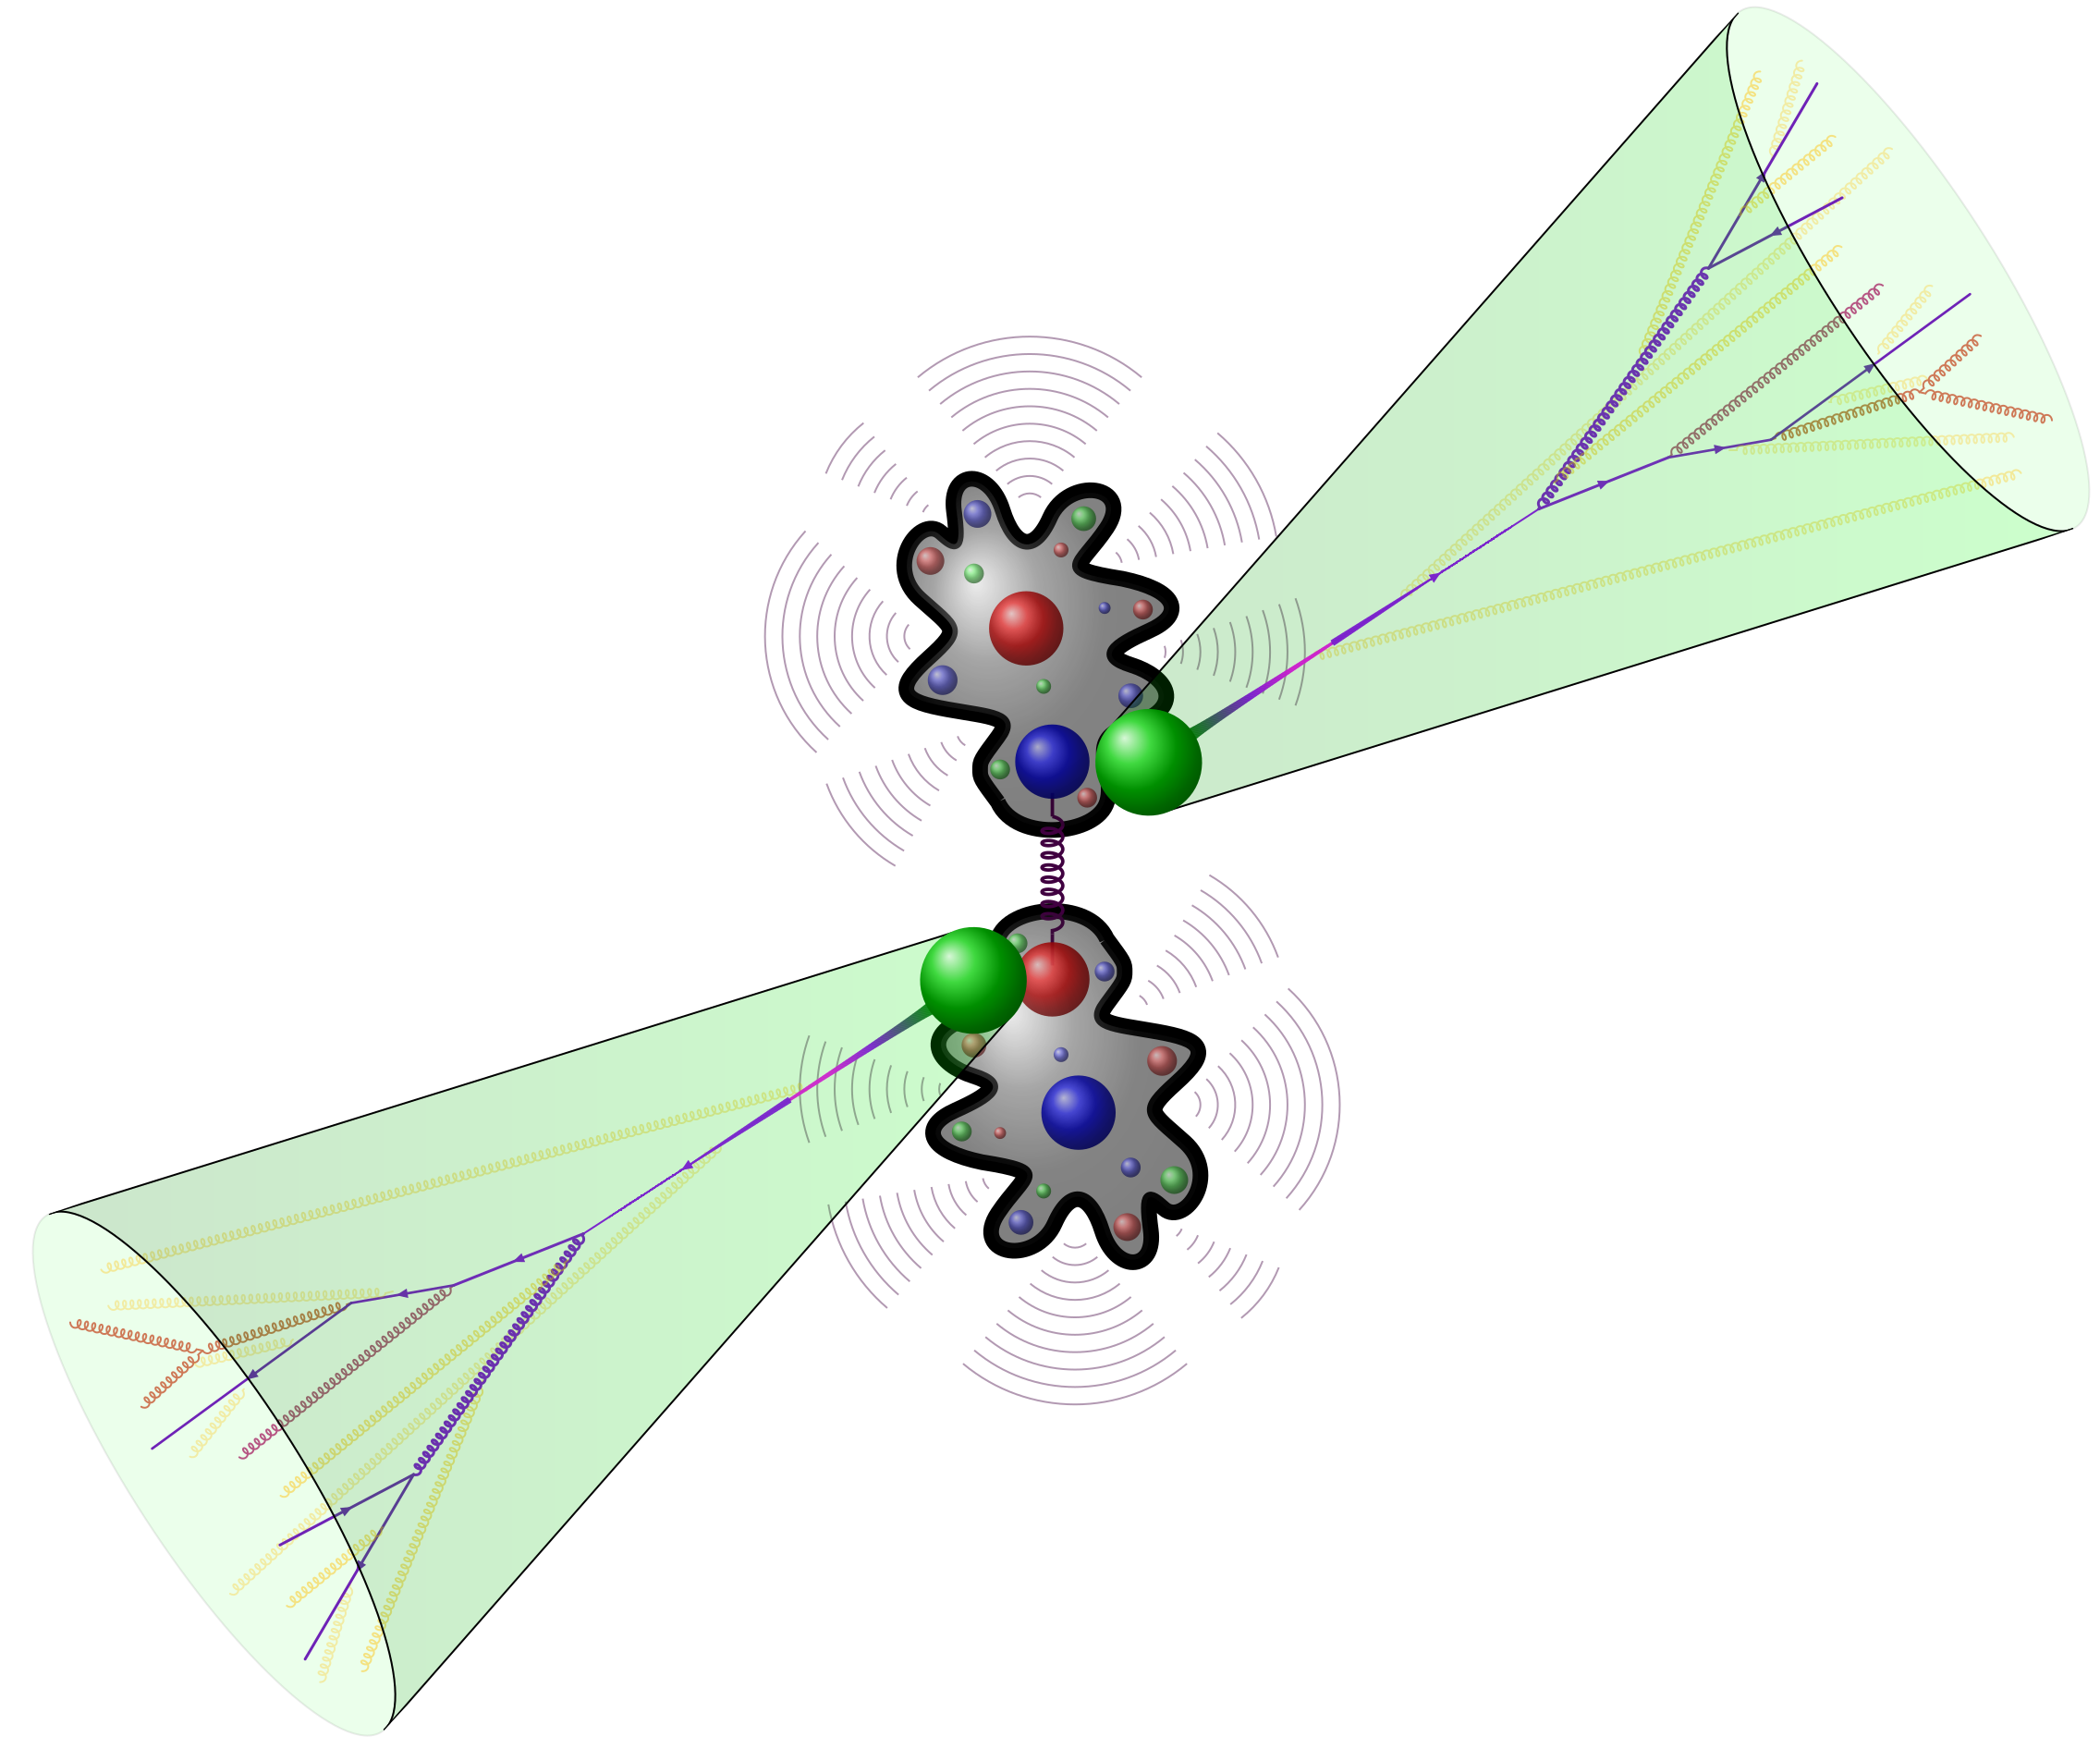
\includegraphics[width=0.48\textwidth]{figures/misc/ue-jets}
        \label{fig:app-ue}
    }
    \subfloat[]{
        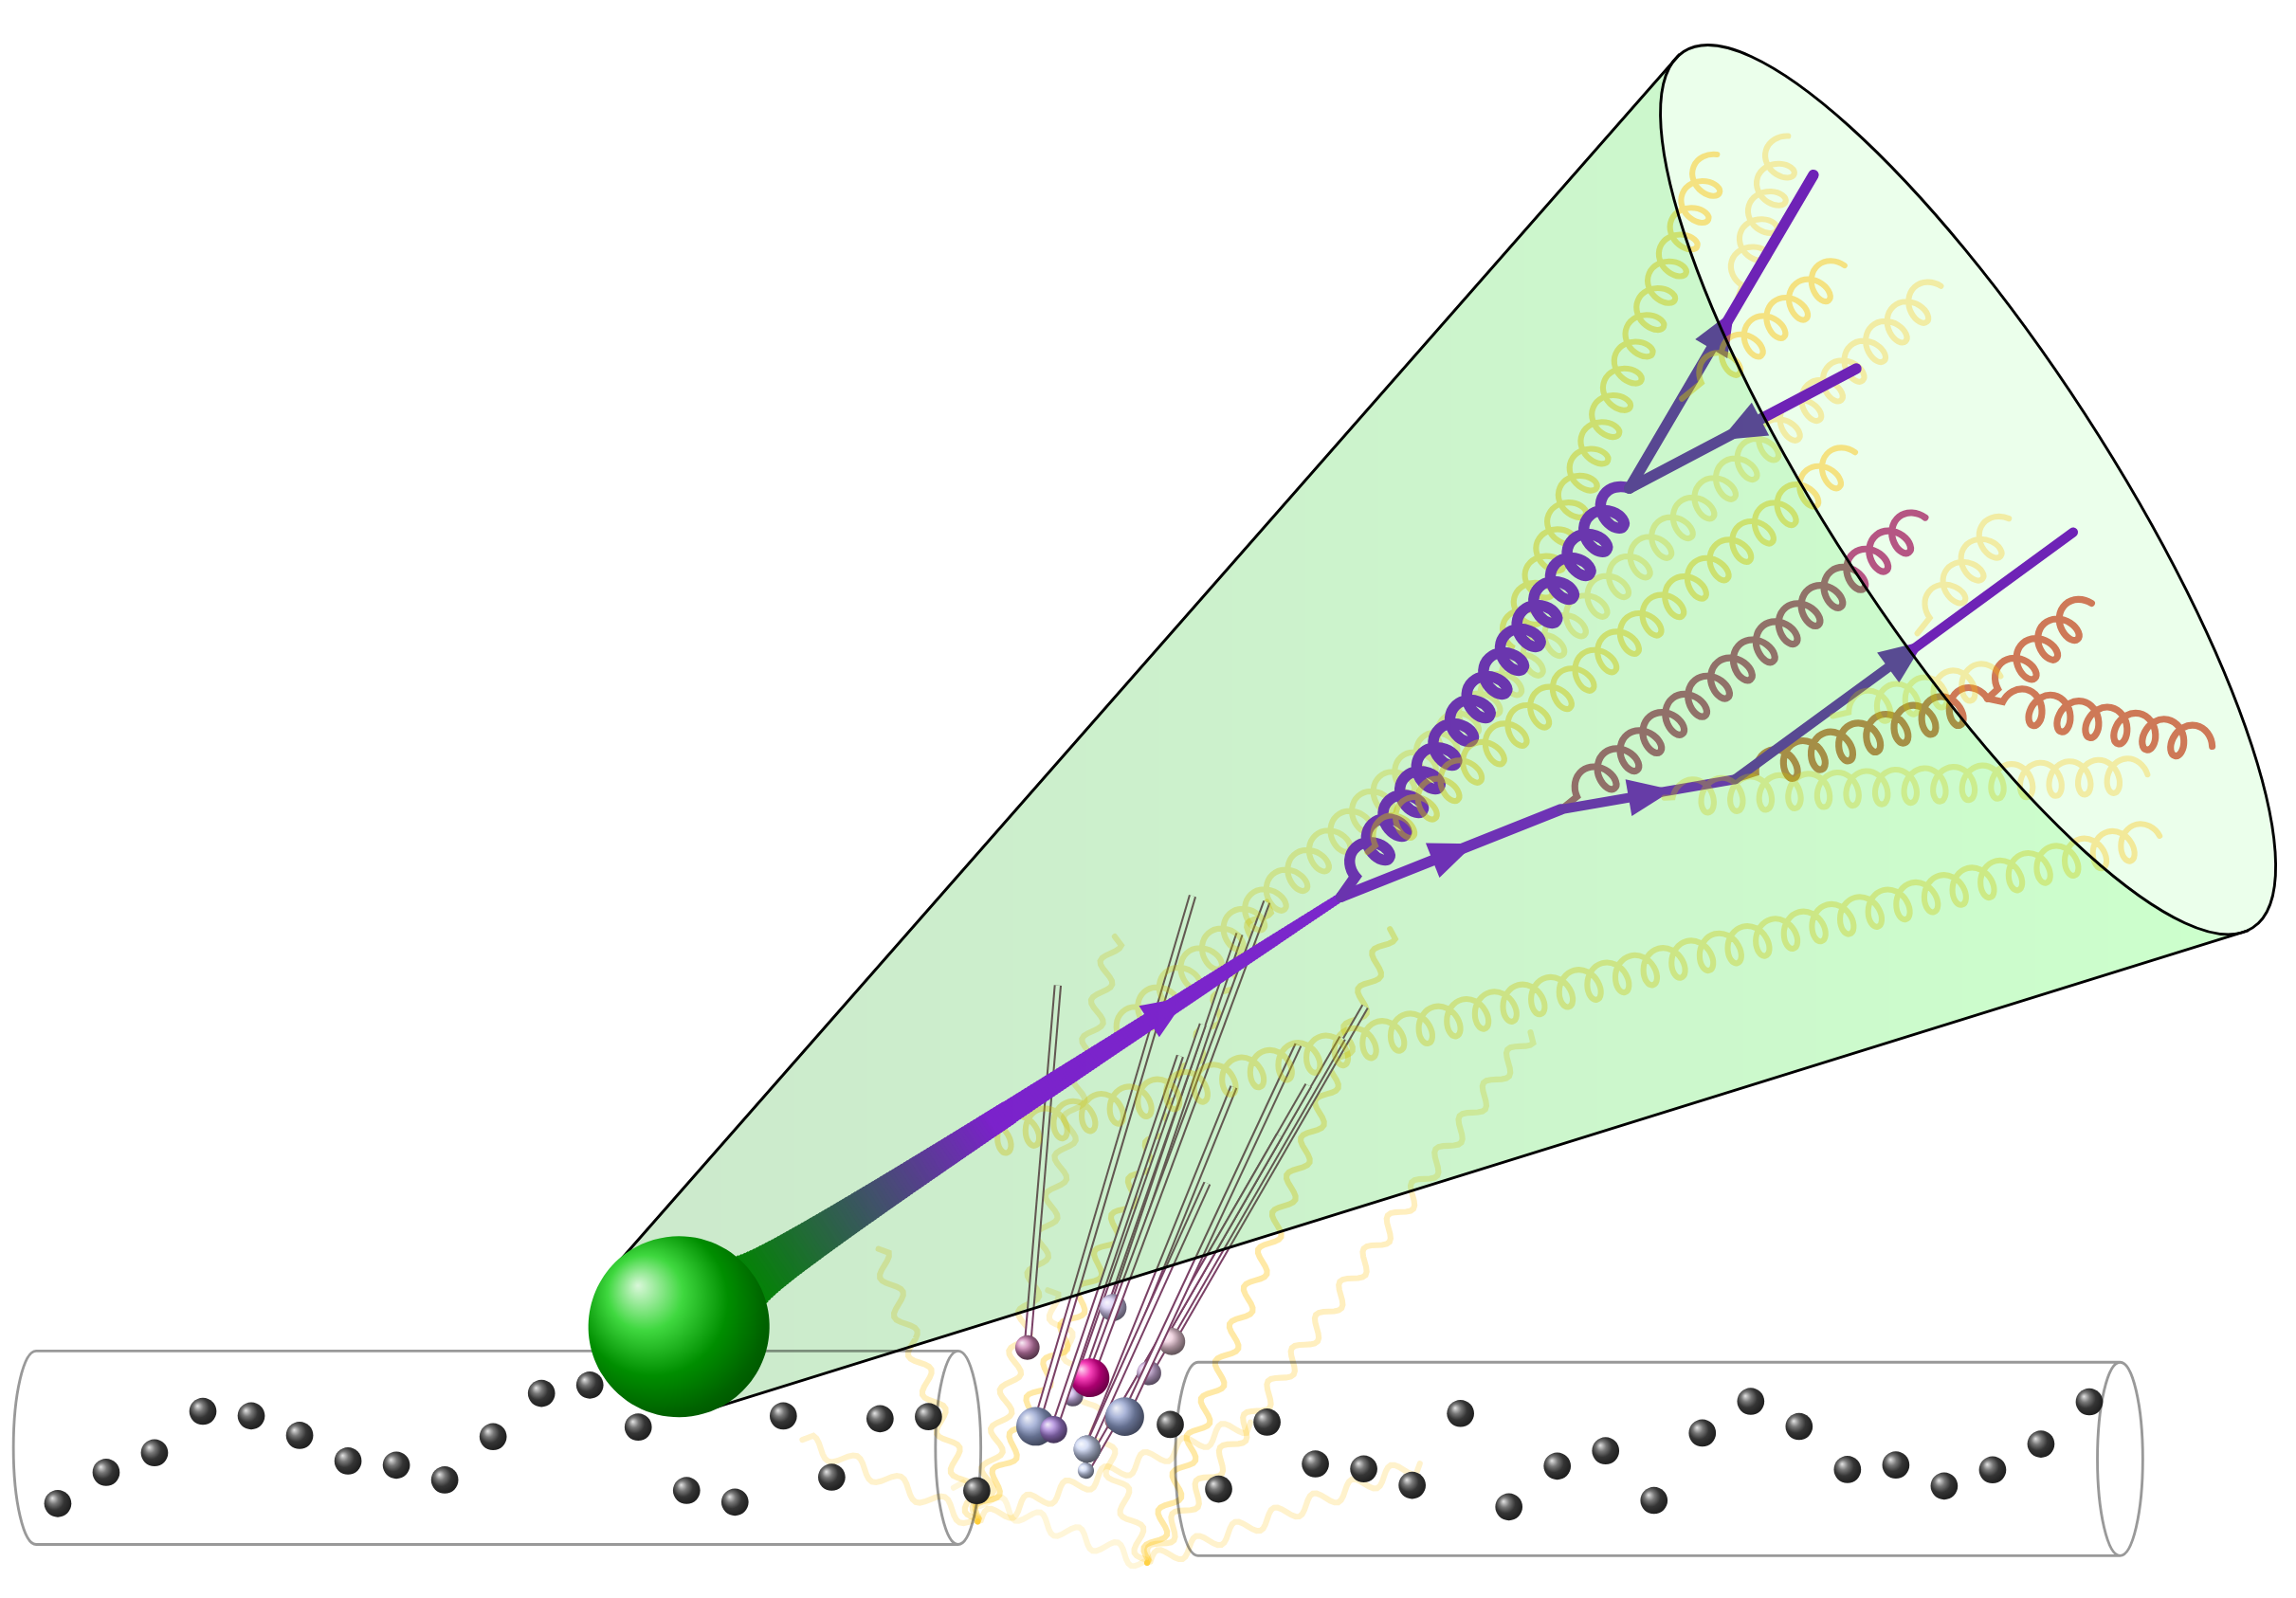
\includegraphics[width=0.48\textwidth]{figures/misc/pu-jet}
        \label{fig:app-pu}
    }
    \caption[Visualizations of additive contamination in particle collisions.]{Visualizations of important sources of additive contamination in particle collisions:
    %
    \hyperref[fig:app-ue]{(a)}
    \glslink{ue}{the underlying event (UE)}, described theoretically through additional interactions from partons which are not directly involved in a hard scattering process, and
    %
    \hyperref[fig:app-pu]{(b)}
    \glslink{pileup}{pileup (PU)}, or radiation from lower energy scatterings of \textit{additional} protons not directly involved in a primary hard scattering.
    }
    \label{fig:app-additive-contamination}
\end{figure}


The \glslink{ue}{underlying event (UE)} (see \Fig{app-ue}) is a theoretical source of additive contamination in hadronic collisions whose behavior must be modelled for accurate predictions of jet substructure.
%
The first-principles framework of \gls{ue} is an area of active research, but in this thesis we use the well-understood and highly successful framework of \textit{\glslink{mpi}{multiple parton interactions (MPI)}} in \gls{pythia}.

\begin{definitionbox}{Underlying Event}{ue}
    \vocab{\glslink{ue}{The underlying event (UE)}} is radiation produced in a high-energy hadron collision that is not directly related to the hard scattering process that produces the primary partons or jets.
    %
    The dominant model of \gls{ue} is the \vocab{\gls{mpi}} model of \gls{pythia}.

    In the context of hadronic collisions in \gls{pythia}, \glslink{mpi}{multiple parton interactions} occur when, rather than the collision involving only one parton from each hadron, the more detailed inner structure of the hadrons involving multiple partons is taken into account.
    %
    \gls{mpi} refers to the additional scatterings of these multiple partons (in principle described by generalized \(n\)-parton distribution functions, though the rarity of these additional scatterings means that only 2-parton distribution functions are needed in practice).
\end{definitionbox}



\remark{mpi}{
    The \gls{mpi} model of \gls{pythia} also combines the multiple-parton-scattering model described above with insights from a theoretical description of all-orders effects in scattering (called Regge-Gribov theory, after its creators \cite{Gribov:1967vfb}) in which ``cut pomerons'', beyond the scope of this thesis, contribute to hadronic cross sections through the production of a large number of low-energy gluons.
    %%
    %An understanding of the ideas of Regge-Gribov theory in effective field theory is an area of ongoing research which, to my knowledge, is spearheaded by the framework of Glauber \gls{scet} (see, for example, discussion in Secs. 7.2, 8, and 9, of \Reff{Rothstein:2016bsq}, as well as interesting discussions in \Reffs{Moult:2022lfy,Gao:2024qsg,Gao:2024fyz}).
}


\remark{}{
    The number of multiple-parton interaction vertices in \gls{pythia} is taken to be Poisson-distributed.
    %
    Furthermore, the radiation produced by multiple-parton scatterings is, when averaged, roughly uniform in the rapidity-azimuth plane.
    %
    These simple features allow for the development of tractable phenomenological models for certain features of \gls{ue}.
    %
    A particularly elegant characterization is given by \Reff{Cacciari:2009dp}.
    %
    Among other characterizations of the expected phenomenological behavior of \gls{ue}, they are able to explicitly derive an estimate of the distribution of transverse momenta due to \gls{ue} in a given area of the rapidity-azimuth plane, assuming a Poisson-distributed number of outgoing particles from \gls{ue} and an exponential distribution for their transverse momenta.
    %
    Under these assumptions, they find (in \href{https://arxiv.org/pdf/0912.4926\#page=7}{Section 3.1}, see also \href{https://arxiv.org/pdf/0912.4926\#page=35}{Appendix A} and \href{https://arxiv.org/pdf/0912.4926\#page=7}{footnote 2}) the surprisingly compact result
    \begin{align}
        \frac{\dd P}{\dd p_T^{\rm(UE)}}(A)
        =
        e^{-\nu A}
        \le(
            \delta\le(p_T^{\rm(UE)}\ri)
            +
            e^{-p_T^{\rm(UE)}/\mu}
            \sqrt{\frac{A \, \nu}{p_T^{\rm(UE)}\, \mu}}
            I_1\le(2\sqrt{\frac{A\,\nu\, p_T^{\rm(UE)}}{\mu}}\ri)
        \ri)
        \,,
    \end{align}
    where $I_1$ is a modified Bessel function (of the first kind), \(\nu\) is the parameter which governs the average of the Poisson-distributed number of particles per unit area (\(\nu \sim 5\) is the realistic value they give for \gls{ue} at the LHC), and \(\mu\) is a parameter governing the average of the exponentially-distributed transverse momentum of each individual particle (they give \(\mu \sim\) 0.4 GeV, which they find corresponds to an average \(p_T\)-per-area of about 2 GeV).
    %
    Unfortunately, this elegant result does not make further appearances in this thesis.
}

In this thesis, we look at examples in which we characterize the effects of the underlying event on the distribution of collider observables.
%
A more rigorous analyst would also quantify the \textit{uncertainties} in distributions \textit{due to the modelling of the underlying event}.
%
Analyses of uncertainties due to \gls{ue} modelling -- as performed in experimental analyses -- involves at least the two following steps:
\begin{itemize}
    \item
        \textbf{Reweighting:} (also important for \gls{pileup})

        We have theoretical expectations for the distribution number of multiple-parton interactions, \(N_\text{UE}\), associated with collision events at a certain scale, but we want to quantify our uncertainty about the precise form of the \(N_\text{UE}\) distribution.
        %
        This is achieved by \textit{re-weighting} events -- i.e. re-weighting their contributions to histograms -- based on the effective value of \(N_\text{UE}\).
        %
        We give a simplistic description of re-weighting, in which we assume we have access directly to \(N_\text{UE}\), in Example \ref{ex:reweighting-ue} below.
        %
        In practice, however, re-weighting is performed by re-weighting events by a function of collision parameters that are closely related to \gls{ue}, rather than \(N_\text{UE}\) itself.
        %
        In particular, when simulating \gls{ue} with \gls{pythia}, one can keep track of scales used by the shower algorithm to generate initial-state radiation (ISR) and final-state radiation (FSR) for each collision.
        %
        These are are also correlated with the number \(N_\text{UE}\) of multiple-parton interactions.
        %
        By re-weighting events based on the ISR and FSR scales of the shower, one can effectively change the distribution of \(N_\text{UE}\) associated with the generated events.


    \item
        \textbf{Changing tunes:}

        To characterize uncertainties in other parameters of the \gls{ue} model (usually reserved only for precision measurements), one chooses several, previously tuned/validated values of particular \gls{pythia} parameters controlling \gls{ue} behavior -- called the \vocab{\gls{pythia} tune} -- and examine the differences in the distributions obtained with different tunes.
\end{itemize}

\remark{}{
    In this thesis, we perform no re-weighting, and only present results obtained with the default Monash tune of \gls{pythia} \cite{Skands:2014pea}.
    %
    The \gls{pythia} tune often preferred in experimental analyses is the CP5 tune introduced by the CMS experiment \cite{CMS:2022awf}.
}


\begin{example}
    \label{ex:reweighting-ue}
    While in practice one re-weights based on the ISR and FSR scales recorded by \gls{pythia}, let us imagine a simpler situation in which we can directly keep track of the number of underlying event collisions \(N_\text{UE}\).
    %
    We imagine that \(N_\text{UE}\) is Poisson distributed with some mean \(\nu\);
    %
    however, uncertainties in \(\nu\) lead to uncertainties in distributions obtained with \gls{pythia}.
    %
    If we want to understand the effect of uncertainties in \(\nu\) on a histogram describing the distribution of a collider variable \(X\), we can \textit{re-compute} the distribution of \(X\), but with \vocab{re-weighted} contributions from from events with different values of \(N_\text{UE}\):
    %
    each event fills a histogram bin with a weight \(w(N_\text{UE})\), rather than one as in the original histogram for \(X\).
    %
    The weight is chosen such that the \textit{effective} number of of multiple-parton interactions is Poisson distributed with a \textit{new} mean \(\nu' \neq \nu\), e.g.
    \begin{align}
        \label{eq:re-weighting-ue}
        \nu'
        =
        \le\langle N_\text{UE}\ri\rangle_\text{re-weighted}
        =
        \frac{
            \sum_{\text{events } i}
            N_i w(N_i)
        }{
            \sum_{\text{events } i}
            w(N_i)
        }
        \neq
        \nu
        \,,
    \end{align}
    where \(N_i\) is the number of multiple-parton interactions in event \(i\).
\end{example}

\begin{exercise}
    Design a re-weighting scheme:

    Given a distribution Poisson($\nu$) with mean \(\nu\), find a weight function \(w_{\nu \to \nu'}(N)\) such that a set of data \(\{N_i\}\) drawn from Poisson($\nu$), re-weighted by \(w_{\nu \to \nu'}(N)\), behaves as if it were drawn from the distinct Poisson distribution Poisson($\nu'$).

    \vspace{7pt}

    \texttt{(Hint:)}
    %
    Your result should be a simple ratio.
\end{exercise}


% \begin{figure}[]
%     \centering
%     \includegraphics[width=0.8\textwidth]{example-image-a}
%     \caption{{Re-weighting}}
%     \label{fig:reweighting}
% \end{figure}


An important experimental source of additive contamination in particle collisions is \glslink{pileup}{pileup (PU)} (see \Fig{app-pu}).
%
Pileup occurs when radiation from an unrelated collision is detector together with the jets, or other high-energy information, from a collision of interest.

Unfortunately, pileup is a necessary feature of modern particle collisions if we want to generate enough collision events to learn about the universe.
%
When colliding protons at the LHC, for example, the vast majority of collisions yield ``uninteresting'' results -- that is, results which do not produce the high-energy jets or other high-energy phenomena for which we need collision experiments.
%
In order to see and test interesting physical results, such as the production of the Higgs boson, we therefore need to collide a huge number of protons.
%
By applying very strong and precise electromagnetic fields, we are able to line up a huge number of protons into a \textit{bunch};
%
particle physics experiments then accelerate two bunches of protons towards each other so that we can observe the results of many collisions.

When two bunches cross, we are more likely to see an interesting particle collision occur -- for example, one with high energy jets.
%
However, the interactions of other protons in each bunch produces produce additional final-state particles included in our experimental results.


\begin{definitionbox}{Pileup}{pileup}
    \vocab{\glslink{pileup}{Pileup (PU)}} refers to the additional interactions in a hadron collision due to multiple collisions occurring nearly simultaneously within the same bunch crossing.
    %
    These additional collisions are not directly related to the hard scattering process of interest but nonetheless interfere with measurements of the primary hard-scattering event, especially in high-luminosity environments.
\end{definitionbox}


\remark{}{
    Since the pileup collisions are approximately un-correlated, the number of pileup events \(N_\text{PU}\) polluting a collision of interest is approximately Poisson distributed.
    %
    There are several methods to experimentally determine the distribution of the number of pileup vertices.
    %
    One is by using known properties of the cross-section associated with \gls{pileup} interactions, \(\sigma_\text{PU}\), and the luminosity of the experiment, \(\mathcal{L}\), to write \(\le\langle N_\text{PU}\ri\rangle = \sigma_\text{PU} \mathcal{L}\).
    %
    Another is by measuring the distribution of \vocab{primary vertices} measured in a particle collision.
    %
    Primary vertices are points from which sets of final-state particles seem to emerge, based on more detailed experimental reconstruction, so \(N_\text{PU} = N_\text{primary} - 1\).%
    \footnote{
        Primary vertices lie only along the axis of the colliding proton beams -- the \(z\) axis -- and are separated in the \(z\) direction.
        %
        \emph{Secondary vertices} -- vertices associated with the decay of a particle emerging from a primary vertex -- would instead be located away from the beam (i.e. with \(x, y \neq 0\)).
    }
    %
    Yet another is by measuring the distribution of transverse momentum per unit rapidity-azimuth area and relating this to the number of pileup events;
    %
    since the transverse momentum produced a pileup event is, on average, uniform in the rapidity-azimuth plane \cite{Soyez:2018opl,Monk:2018clo,Sjostrand:1987su,Sjostrand:2014zea,Dasgupta:2007wa,Kirchgaesser:2020poq,Moraes:2007rq,CDF:2015txs,Larkoski:2021hee,Baron:2020xoi,Marzani:2017kqd}, we expect \(p_T / A \propto N_\text{PU}\) for any given event.
}


\glslink{pileup}{Pileup} events are modelled in both theoretical and experimental contexts by generating \vocab{minimum bias events} -- roughly, events which pass a bare minimum of experimental cuts -- using \gls{pythia}.
%
The number \(N_\text{PU}\) of pileup collisions to be added to the simulated collision of interest is drawn from the appropriate distribution, such as the experimentally measured distribution of \(N_\text{primary} - 1\), or a Poisson distribution with the experimentally realistic mean \(\le\langle N_\text{PU}\ri\rangle \sim 20 - 30\) \cite{Soyez:2018opl}.
%
Then, this number of simulated minimum bias events are generated (or loaded from an existing database), and their final-state particles are added to the set of final state-particles of the simulated collision of interest;
%
the resulting set of final-state particles forms the simulated event together with its simulated pollution.

\remark{}{
    Just as in the case of \gls{ue}, uncertainties in the average number of pileup events, or the pileup distribution more generally, are captured in more detailed analyses by re-weighting (though we do not pursue that level of rigor in this thesis).
    %
    Re-weighting to estimate the effects of varying the \gls{pileup} distribution, however, is simpler in practice than re-weighting for \gls{ue};
    %
    since we may directly keep track of the number of minimum bias events we add to every collision, we may re-weight events directly by a function only of \(N_\text{PU}\) (rather than by a function of indirect probes of \(N_\text{PU}\), as in the case of ISR and FSR scales providing indirect probes of \(N_\text{UE}\)).
}

Pileup can significantly affect jet measurements and leads to difficulties in extracting information about jet substructure.
%
\glslink{pileup}{pileup} and the principles of \glslink{pu-mitigation}{pileup mitigation} will play an important role in our pursuit of jet substructure observables which are insensitive to the effects of low-energy pollution.

\begin{definitionbox}{Pileup Mitigation}{pu-mitigation}
    \vocab{\Gls{pu-mitigation}} refers to any strategy for reducing the impact of \glslink{pileup}{pileup} events on hadronic collisions in high-luminosity environments, usually by separating the jets generated by a primary hard scattering from unwanted pileup contributions.
\end{definitionbox}

In the next chapter, we will make the unusual choice to merge the terms \gls{pu-mitigation} and \gls{jet-grooming}.
%
As we discuss in the next chapter, jet grooming is any method which modifies the constituents of a jet in order to reduce the effects of low-energy pollution.
%
Therefore, we describe \gls{pu-mitigation} as a type of \gls{jet-grooming} which aims specifically to remove \gls{additive-contamination}.
\end{subappendices}



% %%%%%%%%%%%%%%%%%%%%%%%%%%%%%%%%%%%%
% Problems
% %%%%%%%%%%%%%%%%%%%%%%%%%%%%%%%%%%%%
\begin{problems}

\makeprob{The No-Emission Probability (Sudakov Form Factor)}{no-emission}{
    Let \(\Pi_i(m^2 \leftarrow Q^2)\) indicate the probability that, within a partonic cascade initiated by a parton of flavor \(i\) and virtuality \(Q\), that there is no pairwise emission of partons with a mass larger than \(m\);
    %
    this is sometimes called a \vocab{Sudakov form factor} or a \vocab{no-emission probability}.

    \begin{enumerate}[label=\alph*)]
        \item
        Using the strongly-ordered limit, argue that
        \begin{align}
            \Pi_i(m^2)
            \approx
            \exp[
                -
                \,
                \int \dd z
                \,\,
                4\as
                \,
                \sum_j p_{j \leftarrow i}(z)
                \,
                \int \frac{\dd \theta}{\theta}
                \,\,
                \,
                \Theta(z\theta^2 > m^2)
            ]
            \,,
        \end{align}
        and identify where the strongly-ordered limit appears in your analysis.

        Repeat your analysis to calculate the probability that there is no pairwise emission of partons with an \textit{angularity} (\(z_\text{soft}\,\theta^\varsigma\)) less than \(e_\varsigma\);

        \item
        Explicitly compute the analytic form of the LL no-emission probability for angularities that you derived in integral form in (a).
    \end{enumerate}
}




\makeprob{The Algorithms for Generating Partonic Emissions}{veto-algorithm}{
    When simulating the partonic cascade, the complicated form of the splitting functions and running coupling make analytic results more difficult to obtain even for simple quantities (such as the \gls{parton-to-parton} of \Sec{p2p-fragmentation}).
    %
    To solve more complicated problems, it is common to use numerical parton showers and random number generation to simulate the generation of emissions in the partonic cascade.
    %
    In this problem, we explore the basics of some simple sampling techniques.


    \begin{enumerate}[label=\alph*)]
        \item
        \vocab{Inverse transform sampling} can be used when we have a probability distribution for a random variable \(X\) whose cumulative distribution \(F(X)\) has a known inverse \(F^{-1}(y)\).
        %
        Inverse transform sampling leverages that it is relatively simple to sample a random variable \(U\) which is uniformly distributed from 0 to 1, and relies on the fact that \(F^{-1}(U)\) can be used to obtain the probability distribution of \(X\).

        \textit{Show that \(F^{-1}(U)\) has the same cumulative probability distribution as \(X\) and use this fact to justify inverse transform sampling.}


        \item
        The \vocab{\gls{veto-algorithm}} allows us to sample from an exponential cumulative distribution of the form
        \begin{align}
            \Pi_f(x\,|\,T) = \exp\le[-\int_x^T \, \dd x' \, f(x')\ri]
            \,,
        \end{align}
        where \(f(x')\) is known and positive semi-definite, but its integral may not be known (this is intentionally reminiscent of \Prob{no-emission}).
        %
        In particular, the veto algorithm, much like the accept-reject algorithm, depends on a reference probability distribution;
        %
        in this case, the reference probability distribution also has an exponential cumulative form, \(\Pi_g(x | T)\), has the probability distribution \(g(x) \Pi_g(x | T)\), and must satisfy \(f(x) \leq g(x)\) for all \(x\).

        The veto algorithm is represented graphically through the flow of code
        \begin{center}
            \raisebox{-\height}
            {
            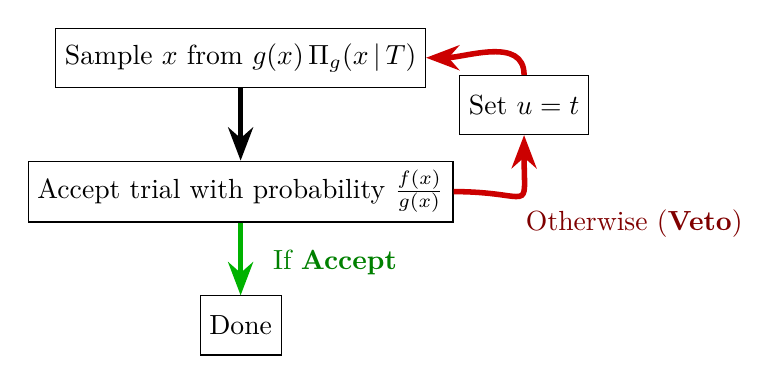
\begin{tikzpicture}
                \node[rectangle, minimum width=1.0cm, minimum height=0.75cm, thin, draw=black] (sample) at (0, 3.4) {Sample $x$ from $g(x) \, \Pi_g(x \, | \, T)$};
                \node[rectangle, minimum width=1.0cm, minimum height=0.75cm, thin, draw=black] (accept) at (0, 1.7) {Accept trial with probability $\frac{f(x)}{g(x)}$};
                \node[rectangle, minimum width=1.0cm, minimum height=0.75cm, thin, draw=black] (done)   at (0, 0.0) {Done};
                \node[rectangle, minimum width=1.0cm, minimum height=0.75cm, thin, draw=black] (veto)   at (3.6, 2.8) {Set $u = t$};


                \draw[black, line width=2pt, -Stealth] (sample) to [out=270,in=90] (accept);
                \draw[red!80!black, line width=2pt, looseness=2.3, -Stealth]   (accept) to [out=0,in=270](veto);
                \draw[red!80!black, line width=2pt, looseness=1.0, -Stealth] (veto) to [out=90,in=0](sample);
                \draw[green!70!black, line width=2pt, -Stealth] (accept) to [out=270,in=90](done);


                \node[green!50!black] at (1.2, 0.8) {If \textbf{Accept}};
                \node[red!50!black] at (5.0, 1.3) {Otherwise (\textbf{Veto})};
            \end{tikzpicture}
        }
    \end{center}

    \textit{Show that the \gls{veto-algorithm} described by the graphic above accurately samples from the desired probability distribution.}
    \end{enumerate}

    \noindent
    (\texttt{Note:} Adapted directly from \Reff{Bierlich:2022pfr}, whose section 2.2 is a wonderful resource for learning about sampling and Monte Carlo algorithms)
}


\makeprob{\(\star\) A Numerical Parton Shower \(\star\)}{parton-shower}{
    Using the results of \Probs{no-emission}{veto-algorithm}, write pseudocode for a parton shower algorithm which generates emissions ordered by angularity, i.e. such that the angularity of any emission is smaller than that of its parent.
}


\makeprob{Recursive Fragmentation Functions}{p2p-fragmentation}{
    As in \Sec{p2p-fragmentation}, let \(F_{j\leftarrow i}(z\,|\,\rsub \leftarrow \Rjet) \,\, \dd z\) denote the probability of finding a parton of flavor \(j\) at an angular scale \rsub, with momentum fraction between \(z\) and \(z + \dd z\) of an initiating parton \(i\) measured at an angular scale \Rjet.

    \begin{enumerate}[label=\alph*)]
        \item
            Derive the recursive fragmentation formula,
            \begin{align}
                \label{eq:feynman_field_fragmentation_formula}
                F_{j\leftarrow i}(z\,|\,\rsub\leftarrow\Rjet)
                \,\,
                =&
                \,\,
                \delta(1-z) \, \delta_{ij}
                \\
                \notag
                &
                \,
                +
                4
                \,
                \int_{\rsub}^{\Rjet} \frac{\dd\theta}{\theta} \,
                \int_z^1 \frac{\dd y'}{y'} \,
                    \,
                    a_s
                    \,
                    \sum_{k'}
                    F_{j\leftarrow k'}(z/y'\,|\,\theta\leftarrow\Rjet)
                    \,
                    p_{k' \leftarrow i}(y')
                \,,
            \end{align}
            through physical intuition.

        \item
            Does \Eq{feynman_field_fragmentation_formula} have the correct behavior at \(\Rjet = \rsub\)?

        \item
            Show that the recursive fragmentation formula also implies the DGLAP equations of \Eq{dglap-equations-parton-shower}, which were derived through a more complete parton shower approach in \Sec{p2p-fragmentation}.
    \end{enumerate}
}


\makeprob{\(\star\star\) Multiple Emissions \(\star\star\)}{multiple-emissions}{
    \begin{enumerate}[label=\alph*)]
        \item
            Write an expression, in terms of an infinite sum over products of phase space factors, for the cumulative distribution of an additive observable \(X\);
            %
            do \textit{not} use the approximation that the value of \(X\) is set by a single emission discussed in \Prop{ll-additive} and \Sec{ll-substructure-diagrams}.

        \item
            By taking a Laplace transform, performing a sum, and taking an inverse Laplace transform, show that the cumulative distribution for the additive observable \(X\) can be written in the form
            \begin{align}
                \Sigma(x)
                \approx
                \frac{\exp[-H(x)]}{\Gamma\le(1 + H'(x)\ri)}
                \,,
            \end{align}
            up to terms of \(\mathcal{O}(H''(x))\), where \(H'(x) := -\dd H(x) / \dd \log(x)\).
            %
            What is \(H(x)\)?

            \texttt{(Hint:)} You may need the formula \(\int_{c-i\infty}^{c+i\infty} \frac{\dd y}{2 \pi i y} e^y y^{-A} = 1/\Gamma(1 + A)\) for the inverse Laplace transform of \(e^y y^{-1-A}\);
            %
            this can be found e.g. in \href{https://arxiv.org/pdf/1809.03933\#page=5}{Lemma 2.1 of} \Reff{schmidt2019shortnoteintegraltransformations}, or \href{https://univ.jeanpaulcalvi.com/Posters/ConfAuchWeb/abramovitz2.pdf\#section.5.9}{Section 5.9 of} \Reff{822801}.

        \item
            Argue that, for small \(x\), \(H(x)\) is approximately given by \(R_X(x)\), and show that this reproduces the correct leading logarithmic features derived in \Sec{ll-substructure-diagrams}.

        \item
            When \(X\) is an angularity, show that
            \begin{align}
                H(x) = R_X(x) + \gamma_E R'(x)
                \,,
            \end{align}
            and therefore that the cumulative distributions of angularities, when multiple emissions are included, take the form
            \begin{align}
                \Sigma(x) \approx \frac{e^{-R(x) - \gamma_E R'(x)}}{\Gamma\le(1 + H'(x)\ri)}
                \,.
            \end{align}

        \item
            Justify our neglect of the terms of \(\mathcal{O}(H''(x))\).
    \end{enumerate}
}




\makeprob{\(\star\) Angularities at modified leading-logarithmic accuracy \(\star\)}{mll-angularities}{
    Using the result of \Prob{multiple-emissions}, and taking into account running coupling effects, write an analytic expression for the MLL cumulative distribution for angularities in jets initiated by a parton of flavor \(i\), and show that it recovers the correct LL result in the limit \(\alphas\to0\).
    %
    Recall that the MLL result should include running coupling effects, multiple emissions, and non-singular pieces of the splitting functions.
    %
    If you are brave, you may also freeze the coupling below a non-perturbative scale.

    \texttt{(Hint:)} Luckily, as discussed at the end of \Sec{ll-substructure-diagrams}, you may assume all contributions are from the primary branch of the jet, so that you will only need to use the form of a single splitting function, \(p_{i g \leftarrow i}(z)\), for each \(i\).
}





\vspace{10pt}
\hrule
\vspace{10pt}


\section*{Problems on the Mellin Transform}


\makeprob{Mellin Convolution Theorem}{mellinconvolution}{ Prove the Mellin Convolution Theorem of Proposition~\ref{prop:mellin-convolution-app}.  }


\makeprob{Mellin Convolution Theorem II}{mellinconvolution2}{
    There is another, related convolution in the context of Mellin transforms.
    %
    Consider the new convolution
    \begin{align}
        (f \circ_{\mc M} g)(x)
        =
        \int_0^\infty\,\dd\xi f(x\,\xi) g(\xi)
        \,.
    \end{align}
    Show that the Mellin transform of this convolution is
    \begin{align}
        \mathcal{M}[f \circ_{\mc M} g](s)
        \,
        =
        \,
        \mathcal{M}[f](s) \, \mathcal{M}[g](1-s)
        =:
        \hat{f}(s) \, \hat{g}(1-s)
        \,.
    \end{align}
}
% \begin{exercise}
%     {BFKL... turn to problem}
    % https://www.hep.phy.cam.ac.uk/theory/webber/QCDlect3.pdf#page=22
% \end{exercise}


% Multiplicity... similar to the techniques of jet calculus, but I first saw it in...
%https://arxiv.org/pdf/1704.06266

\end{problems}
  % TOGGLE
% ==============================================

% ==============================================
\chapter[Removing the Rubble:\\\phantom{Chapter 4:|}Jet Grooming and Cleanup Fish]{Removing the Rubble:\hfill\\Jet Grooming and Cleanup Fish}
\markboth{\small \textsc{Chapter \thechapter}: \bf Removing the Rubble: Jet Grooming and Cleanup Fish}{}

\label{chap:grooming}

% -----------------------------------
% Picturebook figure
% -----------------------------------
\reusefigure[]{picturebook_substructure}


We've now seen jets as proxies for partons, discussed the partonic cascade as a model of jet formation, and given some predictions regarding the jet observables and the flow of energy within jets.
%
We have also seen that there will be difficulties comparing these predictions to experimental results, in the form of low-energy pollution within particle collision events.
%
We now take a first step towards developing soft-insensitive probes of jet substructure, in order to gain information about the flow of energy in the partonic cascade in a more realistic experimental context.

In this chapter, we introduce \textit{\gls{jet-grooming}}:
%
a powerful and conceptually simple set of tools that facilitate our understanding of jet substructure by removing low-energy pollution from jets.
%
The low-energy phenomena of QCD that produce both soft contamination and \gls{additive-contamination} are notoriously difficult to model, and jet grooming has become an important toolkit used to empower both experimental and theoretical analyses of jet substructure
\cite{Krohn:2009th,Ellis:2009me,Larkoski:2014wba,Dasgupta:2013ihk,Dasgupta:2013via,Tseng:2013dva,Dasgupta:2016ktv,Thaler:2008ju,Thaler:2011gf,Hook:2011cq,Gallicchio:2011xq,Soper:2012pb,Gallicchio:2012ez,CMS-PAS-JME-09-001,CMS-PAS-EXO-09-002,CMS:2013kfa,ATL-PHYS-PUB-2009-081,ATL-PHYS-PUB-2010-008,Cui:2010km,ATLAS-CONF-2011-053,Chatrchyan:2013rla,Larkoski:2013eya,Dasgupta:2012hg,Backovic:2013bga,ATLAS-CONF-2013-084,Komiske:2018vkc,Komiske:2016rsd,Metodiev:2018ftz,Krohn:2012fg,MERINO:2013tta,Bhattacherjee:2016bpy,Macaluso:2018tck,Egan:2017ojy,Kasieczka:2017nvn,Pearkes:2017hku,Butter:2017cot,Catani:1992ua,Dokshitzer:1998kz,Dasgupta:2001sh,Banfi:2004yd,Banfi:2005gj,Ellis:2009su,Banfi:2010pa,Walsh:2011fz,Chien:2012ur,Li:2012bw,Jouttenus:2013hs,Hatta:2013iba,Larkoski:2014tva,Procura:2018zpn,Aaboud:2017aca,Frye:2016aiz, Almeida:2008yp,Larkoski:2017iuy,Larkoski:2017cqq,Thaler:2010tr,Abdesselam:2010pt,Katz:2010mr,Gallicchio:2010dq,Adams:2015hiv,Sirunyan:2017ezt,Moore:2018lsr,FerreiradeLima:2016gcz,Rubin:2010fc,Chatrchyan:2012sn,ATLAS:2019kwg,CMS-PAS-BTV-13-001,CMS-PAS-JME-13-006,Kribs:2009yh,Chen:2010wk,Hackstein:2010wk,Kim:2010uj,Almeida:2011aa,Pandolfi:2012ima,Vernieri:2014wfa,CMS-PAS-HIG-17-007,Procura:2014cba,ATL-PHYS-PUB-2019-027,Aad:2019vyi,ATLAS:2020gwe}.
%
Again, I also highly recommend the pedagogical treatment of \Reff{Marzani:2019hun}.



%==============================================
\section{The physical picture}
%==============================================

Examining the substructure of a jet is like peering through a cloud of rock dust or into a cloudy puddle to look for the faint gleam of a gem.
%
In particular, the high-energy structures within jets, which through \gls{asymptotic-freedom} encode partonic degrees of freedom, are obfuscated by a miasma of low-energy pollution.
%
To extract high-energy information encoded by jet substructure, we need to remove the low-energy pollution from \gls{hadronization}, \gls{deteffects}, \glslink{ue}{the underlying event}, and \glslink{pileup}{pileup} obfuscating any modern particle collision.
%
To uncover the physical properties of partons, we need to \textit{isolate} the high-energy structures within jets.


Jet grooming takes a very practical and straightforward approach to the problem of low-energy pollution:
%
it directly removes or modifies low energy particles from jets!
%
Grooming techniques help isolate the high-energy core of the jet that is directly associated with the hard scattering process, leading to cleaner and more accurate measurements of jet substructure.
%
In this context, grooming is crucial for realistic collider studies of QCD and new physics searches.

\begin{definitionbox}{Jet Grooming}{jet-grooming}
    \glslink{jet-grooming}{\vocab{Jet grooming}} is any method that modifies the constituents of a jet -- e.g. by removing, reweighting, or reclustering certain particles -- in order to reduce the impact of \glspl{soft-distortion} and \gls{additive-contamination}.
    %
    Jet grooming usually aims to preserve the information associated with the high-energy partonic physics of jet production.
\end{definitionbox}

The conceptual simplicity of jet grooming is accompanied by several practical benefits.
%
Jet grooming can be used to address many sources of low-energy pollution at once, leading to simple analyses that yield robust experimental jet substructure results.
%
Appropriately designed jet grooming strategies can even facilitate analytic calculations of jet substructure observables that may have otherwise involved complicated regions of phase space, or allow the analytic prediction of traditionally mystifying \gls{hadronization} effects \cite{Larkoski:2014wba}.


Jet grooming must also be computationally efficient.
%
High-energy particle accelerators collect data from \textit{more than 500 million collision events every second}.%
\footnote{
    This is a concern because jet grooming is used in experimental trigger systems, which filter among these half-a-billion events which ones should be stored in the memory of a particle collision database.
    %
    The given number is from \href{http://lhc-machine-outreach.web.cern.ch/collisions.htm}{\texttt{the CERN website}}, and does not account for fluctuations in the number of collisions.
}
%
In order to meet the needs of modern particle physicists, jet grooming algorithms must be as fast as possible in order to parse through our vast mountains of data.


There is one final feature we will discuss that is desirable for jet grooming procedures, but that is deceptively difficult to achieve:
%
\textit{continuity}.


The principle of \gls{lphd} (discussed in \Sec{phd}) suggests that small changes in hadronic energy flow should be associated with small changes in the associated partonic degrees of freedom, and vice versa.
%
Therefore, we will hope to achieve a way of isolating high-energy, partonic information in a \textit{continuous} way:
%
small changes in the flow of energy within a jet should not drastically affect what we infer about partonic degrees of freedom.
%
Conversely, a jet grooming algorithm is \textit{discontinuous} if small changes in the properties of jet constituents, such as their energies or angular positions, can lead to extensively different groomed results.

The more specific examples of \textit{soft continuity} and \textit{angular continuity}, mentioned briefly in Remark~\ref{rem:continuity}, will play a significant role in this chapter:
\begin{definitionbox}{Soft and Angular Continuity}{}
    A collider observable \(X\) is \vocab{\glslink{soft-discontinuity}{soft continuous}} (\vocab{\glslink{angular-discontinuity}{angularly continuous}}) if it is continuous with respect to changes in the energies (angles) of final-state particles.

    Conversely, a collider observable \(X\) is \vocab{soft discontinuous} (\vocab{angularly discontinuous}) if infinitesimal changes in the energies (angles) of final-state particles can cause large changes in the value of \(X\).
\end{definitionbox}
\noindent
We will provide more precise definitions of continuity in \Sec{emd}, where we discuss the continuity of grooming algorithms as maps on the space of energy flows.



Unfortunately, traditional jet grooming algorithms are discontinuous, as we discuss in detail in \Sec{discontinuity} (and as in, for example, \Reffs{Dasgupta:2013ihk,Larkoski:2014wba}).
%
Discontinuous behavior in jet grooming algorithms leads in turn to undesirably sensitive responses to low-energy pollution.
%
Experimentally, discontinuities in grooming lead to large responses of groomed substructure to the interactions of jets with experimental detectors, and resulting difficulties in unfolding \cite{ATL-PHYS-PUB-2019-027,Aad:2019vyi,ATLAS:2020gwe}.
%
Theoretically, discontinuities in grooming lead to uncertainties in fixed-order calculations \cite{Larkoski:2014wba} and complications in describing the effects of \gls{hadronization} on groomed jet substructure \cite{Hoang:2019ceu}.


In order to create continuous methods for extracting high-energy information from jets, we introduce the paradigm of Pileup and Infrared Radiation Annihilation (\PIRANHA{}) for \emph{continuous jet grooming}, introduced by myself and my collaborators in \Reff{Alipour-Fard:2023prj}.
%
The \PIRANHA{} paradigm utilizes lessons from traditional jet grooming together with geometric intuition from optimal transport -- see e.g. \Sec{emd} -- in order to generate more continuous grooming strategies, with better formal and phenomenological behavior.
%
However, though we achieve the goal of continuous grooming through the framework of \PIRANHA{}, we will see that as we make grooming procedures which are more and more continuous, they become less and less malleable for interpretation in perturbative calculations.
%
Indeed, without some very subtle work, \textit{any} grooming procedure which attempts to utilize the tree-like structure of partonic emissions discussed in the previous chapter will be necessarily discontinuous (see \Sec{ang_discont}).


\remark{jet-discontinuity}{
    All observables depending on a jet definition are technically angularly discontinuous because the angles between particles determine, discontinuously, whether a jet algorithm reconstructs them as ling within the same jet.
    %
    Therefore, whenever we use the terms ``soft (angular) continuous'', we implicitly mean ``soft (angular) continuous up to discontinuities associated with jet boundaries/the jet definition itself.''
}


\begin{table}[t]
    \centering
    \begin{tabular}{|c|c||c|c||c|c|}
\hhline{~~--||--}
\multicolumn{2}{c|}{}
&
\multicolumn{2}{c||}{Safety}
&
\multicolumn{2}{c|}{Continuity}
\\
\hhline{~~--||--}
\noalign{\vskip\doublerulesep
         \vskip-\arrayrulewidth}
\hhline{--||--||--}
    Groomer & Acronym &
    Infra-red & Collinear &
    Soft & Angular
\\
\hhline{--||--||--}
\noalign{\vskip\doublerulesep
         \vskip-\arrayrulewidth}
\hhline{--||--||--}
Apollonius Subtraction & P-AS &
\cmark & \cmark &
\cmark & \cmark
\\
\hhline{--||--||--}
Iterated Voronoi Subtraction & P-IVS &
\cmark & \cmark &
\cmark & \cmark
\\
\hhline{--||--||--}
Recursive Sub. w/Fraction \(f = 1/2\) & \PRSF{1/2} &
\cmark & \cmark &
\cmark & \danger
\\
\hhline{--||--||--}
Recursive Sub. w/Fraction \(f \neq 1/2\) &  P-RSF\(_{f \neq 1/2}\) &
\cmark & \cmark &
\danger & \danger
\\
\hhline{--||--||--}
\noalign{\vskip\doublerulesep
         \vskip-\arrayrulewidth}
\hhline{--||--||--}
Soft Drop (SD), \(\beta_{\rm SD} > 0\) & SD\(_{\beta > 0}\) &
\cmark & \cmark &
\xmark & \danger
\\
\hhline{--||--||--}
SD (grooming mode), \(\beta_{\rm SD} \leq 0\) & SD\(_{\beta \leq 0}\) &
\cmark & \xmark &
\xmark & \danger
\\
\hline
\end{tabular}


    \caption[Safety and continuity properties of the \PIRANHA{} and Soft Drop grooming algorithms.]{
    Safety and continuity properties of the \PIRANHA{} and Soft Drop grooming algorithms studied in this chapter.
    %
    The mark \cmark~indicates that a groomer satisfies the associated condition, while the mark \xmark~indicates that it does not.
    %
    The mark \raisebox{0.15 em}{\danger} indicates that a groomer does not satisfy the condition, but only in a boundary region of phase space that is exponentially suppressed at leading order in perturbative QCD.
    }
    \label{tab:groomerlist}
\end{table}

\Tab{groomerlist} expresses the infra-red/collinear safety (using the definition of \Reff{Komiske:2020qhg}) and soft/angular continuity properties of the traditional and \PIRANHA{} groomers we discuss in this paper.
%
The soft continuity properties expressed in \Tab{groomerlist} are simple to understand by comparing the hard-cutoff framework of popular groomers to the subtractive framework of \PIRANHA{}.
%
The angular discontinuities expressed in \Tab{groomerlist} are more subtle and are inherited from angular-ordered jet clustering.
%
We note that the Recursive Subtraction algorithms (P-RS) we introduce are discontinuous only in a highly suppressed region of phase space, and we still find it suitable to call P-RS a family of \PIRANHA{} groomers.


In the remainder of the chapter, we show that grooming can provide a useful and intuitive way to extract high-energy information from jet substructure.
%
We exposit the physics of traditional, hard-cutoff grooming in \Sec{traditional-grooming} before exploring \PIRANHA{} strategies for continuous grooming in \Sec{piranha}.
%
We emphasize the improved continuity of \PIRANHA{} formally in \Sec{discontinuity} and in practical applications in \Sec{grooming-pheno}.





%==============================================
\section{Seeing Deep by Keeping Clean: Traditional Jet Grooming}
%==============================================
\label{sec:traditional-grooming}

    % These grooming methods are essential in ensuring that the jet substructure measurements are more representative of the original parton shower, particularly in high-luminosity environments where \glslink{pileup}{pileup} is a significant challenge.


% \begin{remarkbox}{Grooming for Quark-Gluon Discrimination}{}
%     One of the primary applications of jet grooming is to improve quark-gluon discrimination. Quark jets tend to be more collimated with fewer subjets, while gluon jets are broader and more multi-pronged. Grooming techniques such as trimming and pruning remove soft radiation that could distort the substructure, making it easier to distinguish between quark- and gluon-initiated jets. This discrimination is particularly useful for searches in particle physics, where understanding the partonic origin of jets can shed light on underlying processes.
% }

% \begin{remarkbox}{Impact of Jet Grooming on Pileup Mitigation}{}
%     Pileup radiation, which results from additional proton-proton collisions, can have a significant impact on jet substructure in high-luminosity environments. Grooming algorithms are specifically designed to mitigate this effect by removing low-energy particles and focusing on the core hard-scattering part of the jet. For instance, trimming removes soft and wide-angle radiation from \glslink{pileup}{pileup} interactions, thus improving the resolution of jet observables and reducing the bias introduced by \glslink{pileup}{pileup}. As a result, groomed jets are more reliable in precision measurements, such as the study of top quarks and Higgs bosons.
% }


A traditional and elegant approach to jet grooming is to provide a hard cutoff on the energy of the radiation within a jet;
%
this approach retains high-energy information, removes radiation that may be sensitive to \glspl{soft-distortion} or due to \gls{additive-contamination}, and even facilitates perturbative calculations of jet substructure observables.


In this section, we introduce traditional hard-cutoff techniques for jet grooming, discuss their properties, and understand some analytic features of traditionally-groomed jets.
%
We begin with an extremely simple -- and not impractical -- grooming procedure that is nonetheless similar to more complicated algorithms.
%
We then focus on \glsentrylong{soft-drop} -- an algorithm for jet grooming which is extremely popular due to its simplicity, efficiency, and flexibility.%
\footnote{
    Other traditional grooming algorithms include filtering, trimming, pruning \cite{Dasgupta:2013ihk}, and some algorithms for boosted object tagging \cite{CMS-PAS-JME-09-001}, and have similar formal properties to Soft Drop -- including the use of reclustering and the presence of discontinuous behavior.
}

Traditional jet grooming algorithms are discontinuous, but we will only briefly touch on the effects of their discontinuous behavior in this section.
%
Therefore, readers familiar with hard-cutoff jet grooming algorithms such as Soft Drop may want to skip to \Sec{discontinuity}, where we discuss the soft discontinuities of the Soft Drop algorithm.
%
In \Sec{grooming-pheno}, we will see the enormous effects of discontinuities in practical applications.


% ---------------------------------------
\subsection{The Constant Cutoff: An Invitation to Jet Grooming}
% ---------------------------------------
\label{sec:constant-cutoff}

The goal of jet grooming is the efficient removal of low-energy pollution.
%
A simple strategy is to throw away any jet constituents with an energy \(E < E_\text{cut}\), for some constant \(E_\text{cut}\).
%
This is a reasonable first step, and indeed removes low energy radiation to form a resulting groomed jet.

However, we can develop a better algorithm which leverages the tree structure of the partonic cascade and is therefore more amenable to resummed calculations.
%
Instead ignoring particles with \(E < E_\text{cut}\), we will re-cluster the jet to produce a tree-structure representative of the partonic cascade.
%
Then, we will recursively \glslink{declustering}{de-cluster} the jet, throwing out branches of the jet tree with a soft energy fraction less than a pre-defined threshold, \(z < \zcut\).
%
We call this algorithm the \textit{\gls{constant-cutoff}} algorithm for jet grooming.


\begin{definitionbox}{Constant Cutoff Grooming Algorithm}{constant-cutoff}
    The \vocab{constant cutoff grooming algorithm} is a map which takes in a jet and returns a new, \textit{groomed} jet.
    %
    It depends on a single parameter \(\zcut \in (0, 1/2)\).

    The constant cutoff algorithm acts on a jet via the following procedure:
    \begin{enumerate}
        \item
            Re-cluster the jet using the angular-ordered C/A algorithm, as discussed in \Sec{reclustering}, and begin \gls{declustering} the jet tree, starting at the base;

        \item
            If the current branch is a final state particle and cannot be \glslink{declustering}{de-clustered}, stop the algorithm;
            %
            otherwise \glslink{declustering}{de-cluster} the current branch into a softer emission with energy fraction \(z\) of the current branch, and a harder emission with energy fraction \(1-z\);

        \item
            If \(z < \zcut\), remove the softer branch from the jet and continue the algorithm recursively by declustering the remaining, harder branch, as in Step 2;

        \item
            Otherwise, if \(z \geq \zcut\), continue recursively by \gls{declustering} \textit{both} the softer and the harder branch.
    \end{enumerate}
\end{definitionbox}

    The constant cutoff grooming algorithm removes the results of any particularly soft partonic emissions from the jet.
    %
    Its recursive definition in terms of the energy fractions \(z\) of a \glslink{reclustering}{re-clustered} jet tree facilitates resummed calculations, allowing us to model its action on jets through its action on the LL tree of partonic emissions.
    %
    This toy jet grooming example is quite similar to Soft Drop, a widely used grooming algorithm explored in \Sec{softdrop}, and will be a nice playground for building intuition.
    %
    Indeed, the constant cutoff grooming algorithm is the \(N \to \infty\) limit of recursive Soft Drop with \(\betasd=0\) \cite{Dreyer:2018tjj}.

\begin{exercise}{}{}
    Is the \gls{constant-cutoff} algorithm an \glslink{irc-safety}{IRC safe} collider observable?
\end{exercise}



%\remark{}{
%    %
%    Low-energy degrees of freedom are very likely to be groomed by the constant cutoff algorithm;
%    %
%    while \(z > \zcut\) does not imply \(E > E_\text{cut}\) for any value of \(E_\text{cut}\),
%    %
%    however, the inclusion of low-energy degrees of freedom in the groomed jet is extremely unlikely due to the soft singularities of \gls{pqcd}.
%}


\remark{}{
    Treating the \gls{constant-cutoff} grooming algorithm as a map from jets to jets, we can already anticipate its discontinuous behavior:
    %
    if an emission of the jet tree has an energy fraction of exactly \(z = \zcut\), then a miniscule change in energy could lead to it having an energy fraction \(z = \zcut - \epsilon < \zcut\) instead.
    %
    Therefore, while the soft emission with \(z = \zcut\) is not groomed, a small change in the energy distribution of the jet could lead to the soft emission being entirely removed.
    %
    Tiny changes in the energy flow of the jet can lead to macroscopic, discontinuous changes in the structure of the resulting groomed jet.
}


    The \gls{constant-cutoff} grooming algorithm is an example of the general category of \vocab{\glspl{hard-cutoff-groomer}}:
    %
    grooming algorithms (maps from ungroomed jets to groomed jets) which implement a \textit{hard-cutoff}.
    %
    As in the constant cutoff algorithm, which enforces \(z > \zcut\) for the radiation in the groomed jet, a hard cutoff is a condition on the properties of the particles included in the groomed jet which involve an inequality.


\remark{}{
    Since inequalities are discontinuous (for example, \(z > \zcut\) is a discontinuous function from \(z\) to the set \{True, False\}), \glspl{hard-cutoff-groomer} are generically discontinuous as well.
    %
    We say that the constant cutoff algorithm exhibits a \gls{soft-discontinuity} because the addition of very small amounts of energy can discontinuously change the result of the grooming.
}


Since the \gls{constant-cutoff} grooming algorithm leverages the tree-like structure of the partonic cascade, we can use the technology of \Sec{ll-substructure-diagrams} to calculate probability distributions for additive observables in constant-cutoff-groomed jets.
%
The LL probability distribution for additive observables in the groomed jet is similar to that of ungroomed jets, as specified in Proposition \ref{prop:ll-additive} and \Eq{ll-additive}, which we repeat here for convenience:
\begin{align}
    \label{eq:ll-groomed-additive}
    \Sigma^{\text{(LL)}}_X(x; \zcut) \approx \mathbb{P}(X_i < x \text{ for all } i)
    \,.
\end{align}
%
The only difference is that we now have \(X_i = 0\) for \(z_i < \zcut\).%
\footnote{
    The energy fraction \(z'\) after grooming will be zero if \(z < \zcut\), and additivity requires \(X \big|_{z' = 0} = 0\).
}


\begin{example}
    \label{ex:constant-cutoff-mass}
    Let us warm up by computing the mass distribution of constant-cutoff-groomed jets.
    %
    % Using the properties of \glspl{plus-fn} as in \Sec{ll-substructure-diagrams},
    The contribution of a single emission to the observable depends on the groomed energy fraction \(z'\), and takes the approximate form
    \begin{align}
        X(z, \theta)
        =
        m^2(z,\theta)
        \approx
        Q^2 \, z'\,\theta^2
        =
        \begin{cases}
            0 & z < \zcut\,,
            \\
            Q^2 \, z\theta^2 & z > \zcut
            \,.
        \end{cases}
    \end{align}

    Therefore, the cumulative distribution at LL can be written
    \begin{equation}
    \begin{aligned}
        \label{eq:LL_mass_sd}
        \Sigma^{\rm(LL)}_{m^2}(m^2)
        =
        \sum_{n = 0}^{\infty}\frac{1}{n!}
        \Bigg(
        \frac{\alpha_s}{\pi}
        \int_0^R \frac{\dd\theta}{\theta}
        \int_0^{\frac{1}{2}} \dd z\,[\bar{p}_i(z)]_+^{[1/2]}
        \Bigg[
            \Theta\left(
                \frac{m^2}{Q^2} > z\theta^2
            \right)
            &
            \Theta\left(z > \zcut\right)
            \\
            \notag
            +
            &\,\,\Theta\left(z < \zcut\right)
        \Bigg]
        \Bigg)^n
        \,.
    \end{aligned}
    \end{equation}
    Using the properties of \glspl{plus-fn} as in \Sec{ll-substructure-diagrams}, we can conclude that
    \begin{equation}
    \begin{aligned}
        \Sigma^{\rm(LL)}_{m^2}(m^2)
        =
        \sum_{n = 0}^{\infty}\frac{1}{n!}
        \Bigg(
        \frac{\alpha_s}{\pi}
        \int_0^R \frac{\dd\theta}{\theta}
        \int_0^{\frac{1}{2}} \dd z\,\bar{p}_i(z)
        \Bigg[
            &\Theta\left(
                \frac{m^2}{Q^2} > z\theta^2
            \right)
            \Theta\left(z > \zcut\right)
            \\
            \notag
            &+
            \,\,\Theta\left(z < \zcut\right) - 1
        \Bigg]
        \Bigg)^n
        \,.
    \end{aligned}
    \end{equation}
    Finally, using that \(1 - \Theta(a) = \Theta(-a)\), we can use \(\Theta(z < \zcut) - 1 = -\Theta(z > \zcut)\) to notice that the integrand contains
    \begin{align}
        \le(
        \Theta\left(
            \frac{m^2}{Q^2} > z\theta^2
        \right)
        - 1
        \ri)
        \times
        \Theta\left(z > \zcut\right)
        =
        \Theta\left(
            z\theta^2 > \frac{m^2}{Q^2}
        \right)
        \times
        \Theta\left(z > \zcut\right)
        \,.
    \end{align}

    The LL cumulative distribution for the groomed mass can then be written simply as
    \begin{align}
        \Sigma^{\rm(LL)}_{m^2}(m^2)
        =
        \exp\le[-
            \frac{\alpha_s}{\pi}
            \int_0^R \frac{\dd\theta}{\theta}
            \int_0^{\frac{1}{2}} \dd z\,\bar{p}_i(z)
            \,\,
            \Theta\left(
                z\theta^2 > \frac{m^2}{Q^2}
            \right)
            \Theta\left(z > \zcut\right)
        \ri]
        \,.
    \end{align}

I find it helpful to write this in terms of \glspl{substructure-diagram}, since they directly illustrate the behavior of the available phase space for emissions contributing to the cumulative distribution for different regimes of \(m^2\):
\begin{align}
    \Sigma^{\rm(LL)}_{m^2}(m^2)
    =
    \begin{cases}
        \exp\Bigg[
            ~-~
            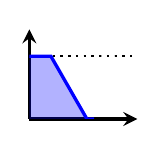
\begin{tikzpicture}[
            baseline={([yshift=-5pt]current bounding box.center)},
            vertex/.style={anchor=base,
            circle,fill=black!25,minimum size=18pt,inner sep=2pt},
            scale=.2]
            \begin{axis}
            [xmin=0, xmax=5,
            ymin=0, ymax=5,
            axis line style = very thick,
            axis y line*=left,
            axis x line*=bottom,
            axis lines = middle,
            ticks=none]
                \addplot[domain=0:5.0,
                style=thick,dotted]
                {3.5};
                \addplot[name path=f,domain=0:3.0,
                style=very thick,blue]
                coordinates {
                    (0,3.5) (1.0,3.5)
                    (2.667, 0) (3.0,0.0)
                };
                \path[name path=axis]
                (axis cs:0,0) -- (axis cs:3.0,0);
                \addplot [
                    thick,
                    color=blue,
                    fill=blue,
                    fill opacity=0.3
                ]
                fill between[
                    of=f and axis
                ];
            \end{axis}
            \end{tikzpicture}
            ~~
        \Bigg]
        & m^2 < \zcut Q^2
        \,,
        \\
        \exp\Bigg[
            ~-~
            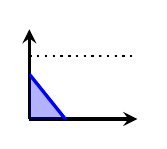
\begin{tikzpicture}[
            baseline={([yshift=8pt]current bounding box.center)},
            vertex/.style={anchor=base,
            circle,fill=black!25,minimum size=18pt,inner sep=2pt},
            scale=.2]
            \begin{axis}
            [xmin=0, xmax=5,
            ymin=0, ymax=5,
            axis line style = very thick,
            axis y line*=left,
            axis x line*=bottom,
            axis lines = middle,
            ticks=none]
                \addplot[domain=0:5.0,
                style=thick,dotted]
                {3.5};
                \addplot[name path=f, domain=0:5,
                style=very thick, blue]
                {2.5-1.5*x};
                \path[name path=axis]
                (axis cs:0,0) -- (axis cs:1,0);
                \addplot [
                    thick,
                    color=blue,
                    fill=blue,
                    fill opacity=0.3
                ]
                fill between[
                    of=f and axis
                ];
            \end{axis}
            \end{tikzpicture}
            ~~
        \Bigg]
        &
        m^2 > \zcut Q^2
        \,,
    \end{cases}
\end{align}
where the dotted line is the line \(z = \zcut\), and the slopes of the diagonal lines in both cases of the substructure diagram are \(-2\) (for constant \(m^2 \approx Q^2 \, z \theta^2\), \(\log(1/z) \approx \text{const} - 2 \log(1/\theta)\)).

Using the singular pieces of the splitting functions and keeping only leading logarithmic terms in \(\log(m^2/Q^2)\) then yields the LL result, for a jet initiated by a parton of color representation \(R\),%
\footnote{
    The result including non-singular pieces of splitting functions can be found e.g. in \href{https://arxiv.org/pdf/1402.2657\#equation.3.9}{Eq. (3.9)} of \Reff{Larkoski:2014wba} by setting their \(\beta = 0\), \(\alpha = 2\).
}
%
\begin{align}
    \label{eq:ll-cc-mass}
    \Sigma^{\rm(LL)}_{m^2}(m^2)
    =
    \begin{cases}
        \exp\le[
            ~-~
            \frac{\alpha_s C_R}{\pi}
            \log(\zcut)\log(m^2/Q^2)
        \ri]
        &
        m^2 < \zcut Q^2
        \,,
        \\
        \exp\le[
            ~-~
            \frac{\alpha_s C_R}{2\pi}
            \,
            \log^2\le(m^2 / Q^2\ri)
        \ri]
        &
        \zcut Q^2 < m^2 < Q^2 / 2
        \,.
    \end{cases}
\end{align}

\end{example}


\remark{}{
    While the \gls{constant-cutoff} grooming algorithm is itself a collinear unsafe collider observable, the \textit{mass} and \textit{angularity} of a constant-cutoff groomed jet is collinear safe.
    %
    Since masses and angularities are additive, and sums of terms of the form \(z_i \theta_i^\varsigma\) which vanish as \(\theta_i \to 0\), collinear splittings do not change the value of either observable.
    %
    This enables e.g. our resummed calculation of the groomed jet mass distribution.
}

\begin{exercise}
    Perform the analysis of Example \ref{ex:constant-cutoff-mass} for the constant-cutoff-groomed \textit{angularities}:
    \begin{align}
        X(z,\,\theta)
        =
        e_\varsigma(z',\theta)
        =
        \begin{cases}
            0 & z < \zcut
            \,,
            \\
            z\theta^\varsigma & z > \zcut
            \,,
        \end{cases}
    \end{align}
    and obtain the leading contributions to the associated probability distributions by approximating \(\bar{p}(z) \approx 2 C_R / z\) and keeping only terms which are leading in logarithms of \(e_\varsigma\).
    %
    Compare your answer to the leading-logarithmic terms in \href{https://arxiv.org/pdf/1402.2657#equation.3.9}{Eq. (3.9)} of \Reff{Larkoski:2014wba} after setting their \(\beta = 0\), \(\alpha = 2\).
\end{exercise}

\remark{cc-discontinuity}{
    The discontinuity of the \gls{constant-cutoff} grooming algorithm manifests in LL calculations as a \emph{kinds in the radiators} of substructure observables, and associated discontinuities of LL probability distributions (e.g. as in \Eq{ll-cc-mass})
    %
    Unfortunately, the kink in the radiator presents a complication when attempting to achieve computations beyond LL.
    %
    In particular, the formula of \Eq{resummed-multiple-emissions} for the inclusion of multiple-emissions effects on cumulative distributions of additive observables depends on the derivative of the radiator.
    %
    We repeat it here for convenience:
    \begin{align}
        \Sigma_X(x)
        &=
        \frac{\exp\le(-R_X(x) - \gamma_E R'_X(x)\ri)}{\Gamma\le(1 + R'_X(x)\ri)}
        \,,
    \end{align}
    where \(R'\) denotes the negative logarithmic derivative of \(R\).
    %
    Therefore, probability distributions which leverage \Eq{resummed-multiple-emissions} depend on the \textit{second derivative} of the radiator.
    %
    Though the radiator turns out to have a well defined derivative, e.g. in \Eq{ll-cc-mass}, it is not second-differentiable, and it is more difficult to account for multiple-emissions effects in \glslink{hard-cutoff-groomer}{hard-cutoff-groomed} jet observables than in ungroomed jet observables.
}



Another set of important collider observables that characterize groomed jet substructure are obtained by focusing on the first emission to survive an angular-ordered grooming procedure:

\begin{definitionbox}{Critical Emission}{}
    The \vocab{\gls{crit-emission}} is the first soft branch of a jet to survive a grooming algorithm based on angular-ordered \gls{declustering}.
    %
    As a result, it is associated with the branching of the groomed jet tree which is widest in angle.

    We call the angle associated with the splitting of the critical emission the \vocab{critical angle} \(\thetacrit\);
    %
    is is also called the groomed angle \(\theta_g\) in the literature.

    We call the energy fraction associated with the critical emission \(\zcrit\), also called \(z_g\) in the literature;
    %
    note that \(0 < \zcrit < 1/2\), since the critical emission is defined as the first \textit{soft} branch to survive a grooming procedure.
\end{definitionbox}

\remark{}{
    When relevant, we call any emissions \textit{preceding} the critical emission \vocab{\glspl{precrit-emission}};
    %
    by the principle of angular-ordering, pre-critical emissions are associated with branches of the partonic cascade which are wider than the critical angle:
    \begin{align}
        \theta_\text{pre} > \thetacrit
        \,.
    \end{align}
    %
    We will also refer to any emissions \textit{following} the critical emission \vocab{\glspl{sub-emission}};
    %
    subsequent emissions are associated with narrow branches of the partonic cascade:
    %
    \begin{align}
        \theta_\text{sub} < \thetacrit
    \end{align}
    indeed, at LL, strong \gls{angular-ordering} implies that any subsequent angles are exponentially smaller than the critical angle:
    %
    \(\theta_\text{sub} \ll \thetacrit\).
}

In a constant-cutoff groomed jet, \(\thetacrit\) is a proxy for the first emission in the partonic cascade which satisfies \(z > \zcut\) (similar intuition will hold for \(\thetacrit\) in \gls{soft-drop} groomed jets, as we discuss in the next section).
%
The distribution of \(\zcrit\) is an experimentally accessible probe of the DGLAP splitting functions themselves \cite{Larkoski:2015lea,ALargeIonColliderExperiment:2021mqf}.
%
These observable have a number of practical applications, some of which we will discover ourselves in this chapter, and they are also quite fun to compute on its own.

\begin{exercise}
    Argue that, though \(\thetacrit\) is not formally an additive observable, we may nonetheless use \glspl{substructure-diagram} and \Eq{ll-groomed-additive} to calculate the cumulative distribution for \(\thetacrit\) at LL.
    %
    In particular, defining \(\Sigma^{\text{(LL)}}_{\thetacrit}\) as the LL probability that no emission with \(z > \zcut\) has \(\theta > \thetacrit\), argue that
    % On the other hand, the probability distribution for \(\theta_{\rm crit}\) alone can be quickly read off from the solution to Example \ref{ex:theta_crit}:
    \begin{align}
        \Sigma^{\text{(LL)}}_{\thetacrit}(\theta_{\rm crit})
        =
        \exp\left[
        ~-~
        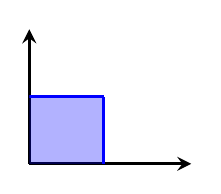
\begin{tikzpicture}[
        baseline={([yshift=-.8ex]current bounding box.center)},
        vertex/.style={anchor=base,
        circle,fill=black!25,minimum size=18pt,inner sep=2pt},
        scale=.3]
        \begin{axis}
        [xmin=0, xmax=5,
        ymin=0, ymax=5,
        axis line style = very thick,
        axis y line*=left,
        axis x line*=bottom,
        axis lines = middle,
        ticks=none]
        	\addplot[name path=f,domain=0:2.3,
            style=very thick,blue]
            {2.5};
            \addplot[very thick, samples=50, smooth,domain=0:6,blue, name path=three] coordinates {(2.3,-1)(2.3,2.5)};
            \path[name path=axis]
            (axis cs:0,0) -- (axis cs:2.3,0);
            \addplot [
                thick,
                color=blue,
                fill=blue,
                fill opacity=0.3
            ]
            fill between[
                of=f and axis
            ];
        \end{axis}
        \end{tikzpicture}
        ~~
        \right]
        \approx
        \theta^{-\frac{2 C_R \alpha_{\rm S}}{\pi}\log(z_{\rm cut}^{-1})}
        ,
        \,.
    \end{align}
    What are the bounds on the associated \gls{substructure-diagram}?

    \label{ex:theta_crit}
\end{exercise}


%A similar analysis yields the cumulative probability distribution function of the angle \(\theta\) for the first emission in the groomed jet that satisfies \(z > \zcut\), which we call the \textit{critical emission}:
%\begin{example}
%    \label{ex:theta_crit}
%    Let's use \glspl{substructure-diagram} to determine the \(\theta_\text{crit}\) distribution in jets groomed with the Constant Cutoff algorithm.
%    %
%    In more words, we want the distribution of the angle of the leading emission of a quark or gluon jet, given that the our emissions also have a minimum-energy-fraction requirement, \(z > z_{\rm cut}\).

%    \begin{center}
%    \begin{tikzpicture}
%    \begin{axis}
%    [xlabel=\(\log(\theta^{-1})\), ylabel=\(\log(z^{-1})\),
%    xmin=0, xmax=5,
%    ymin=0, ymax=5,
%    axis line style = very thick,
%    axis y line*=left,
%    axis x line*=bottom,
%    axis lines = middle,
%    ticks=none]
%        \addplot[name path=f,domain=0:2.3,
%        style=very thick,blue]
%        {2.5};

%        \addplot[very thick, samples=50, smooth,domain=0:6,blue, name path=three] coordinates {(2.3,-1)(2.3,2.5)};

%        \path[name path=axis]
%        (axis cs:0,0) -- (axis cs:2.3,0);

%        \addplot [
%            thick,
%            color=blue,
%            fill=blue,
%            fill opacity=0.3
%        ]
%        fill between[
%            of=f and axis
%        ];

%        \node [rotate=0] at (axis cs:  1.2,  2.8) {$z = z_{\rm cut}$};

%        \node [rotate=0] at (axis cs:  2.95,  1.25) {$\theta = \theta_{\rm crit}$};
%    \end{axis}
%    \end{tikzpicture}
%    \end{center}

%    The corresponding Sudakov factor is
%    \begin{equation}
%    \begin{aligned}
%        \Sigma(\theta_{\rm crit})
%        &\approx
%        \exp\left[
%        ~-~
%        \begin{tikzpicture}[
%        baseline={([yshift=-.8ex]current bounding box.center)},
%        vertex/.style={anchor=base,
%        circle,fill=black!25,minimum size=18pt,inner sep=2pt},
%        scale=.3]
%        \begin{axis}
%        [xmin=0, xmax=5,
%        ymin=0, ymax=5,
%        axis line style = very thick,
%        axis y line*=left,
%        axis x line*=bottom,
%        axis lines = middle,
%        ticks=none]
%        	\addplot[name path=f,domain=0:2.3,
%            style=very thick,blue]
%            {2.5};
%            \addplot[very thick, samples=50, smooth,domain=0:6,blue, name path=three] coordinates {(2.3,-1)(2.3,2.5)};
%            \path[name path=axis]
%            (axis cs:0,0) -- (axis cs:2.3,0);
%            \addplot [
%                thick,
%                color=blue,
%                fill=blue,
%                fill opacity=0.3
%            ]
%            fill between[
%                of=f and axis
%            ];
%            %\node [rotate=0] at (axis cs:  1.2,  2.8) {$z = z_{\rm cut}$};
%            %\node [rotate=0] at (axis cs:  2.95,  1.25) {$\theta = \theta_{\rm crit}$};
%        \end{axis}
%        \end{tikzpicture}
%        ~~
%        \right]
%        =
%        \exp[-\iint_{z > z_{\rm cut},~\theta > \theta_{\rm crit}}
%        \dd\log(\theta) ~~ \dd z ~~ \frac{\alpha_{\rm S}}{\pi} [p(z)]_+ ]
%        \\
%        &\approx
%        \theta^{-\frac{2 C_R \alpha_{\rm S}}{\pi}\log(z_{\rm cut}^{-1})}
%        ,
%    \end{aligned}
%    \end{equation}
%    where in the last line we have used the leading logarithmic expression for the splitting function, as before.
%\end{example}



%\begin{align}
%    \Sigma^{\rm(LL)}_{{\rm crit}, \theta}(\theta_{\rm crit})
%    &=
%    \exp\left[
%        ~-~
%        \begin{tikzpicture}[
%        baseline={([yshift=-.8ex]current bounding box.center)},
%        vertex/.style={anchor=base,
%        circle,fill=black!25,minimum size=18pt,inner sep=2pt},
%        scale=.3]
%        \begin{axis}
%        [xmin=0, xmax=5,
%        ymin=0, ymax=5,
%        axis line style = very thick,
%        axis y line*=left,
%        axis x line*=bottom,
%        axis lines = middle,
%        ticks=none]
%        	\addplot[name path=f, domain=0:2.3,
%            style=very thick, blue]
%            {2.5};
%            \addplot[very thick, samples=50, smooth,domain=0:6,blue, name path=three] coordinates {(2.3,-1)(2.3,2.5)};
%            \path[name path=axis]
%            (axis cs:0,0) -- (axis cs:2.3,0);
%            \addplot [
%                thick,
%                color=blue,
%                fill=blue,
%                fill opacity=0.3
%            ]
%            fill between[
%                of=f and axis
%            ];
%            % z region arrow and label
%            \node [rotate=0] at (axis cs:  2.0,  4.0)
%            {${\scriptstyle z < \zcut}$};
%            \coordinate (I)  at (3.3, 3.4);
%            \coordinate (F)  at (3.3, 4.9);
%            \draw[-Stealth,line width=.2mm] (I) -> (F);
%            % theta region arrow and label
%            \node [rotate=0] at (axis cs:  1.18,  1.38)
%            {${\scriptstyle \theta > \theta_{\rm crit}}$};
%            \coordinate (I)  at (1.8, .5);
%            \coordinate (F)  at (.3, .5);
%            \draw[-Stealth,line width=.2mm] (I) -> (F);
%        \end{axis}
%        \end{tikzpicture}
%        ~~
%    \right]
%    =
%    \exp\left[
%    -\frac{\alpha_s}{\pi}
%    \int_{\theta_{\rm crit}}^R
%    \frac{\dd\theta}{\theta}
%    \int_{\zcut}^{1/2}
%    \dd z\,
%    \bar{p}_i(z)
%    \right],
%\end{align}
%%


Since \(\thetacrit\) is such a pedagogically useful and phenomenologically important observable, we record its probability density ourselves even though the calculation of its properties was the object of the previous exercise:
\begin{equation}
   \rho^{\rm (LL)}_{\thetacrit}(\theta_{\rm crit})
    =
    \frac{1}{\theta_{\rm crit}}
    ~
    \frac{\alpha_s}{\pi}
    \int_{\zcut}^{1/2}
    \dd z\,
    \bar{p}(z)
    \,\,
    \exp\left[
        -\frac{\alpha_s}{\pi} \int_{\theta_{\rm crit}}^R
        \frac{\dd\theta}{\theta}
        \int_{\zcut}^{1/2} \dd z\,
        \bar{p}_i(z)
    \right]
    \,.
\end{equation}
%
The probability distribution for the energy fraction of the critical emission is, at \glslink{accuracy}{NLO}, given simply by a reduced splitting function restricted to the range \(z > \zcut\), with an additional normalization:
\begin{align}
    \label{eq:constant-cutoff-zcrit}
    \rho^{\text{(LO)}}_{\zcrit}(\zcrit)
    =
    \frac{\bar{p}(\zcrit) \,\, \Theta\le(\zcrit > \zcut\ri)}
    {\int_{\zcut}^{1/2} \bar{p}(z)}
\end{align}


The resummed, joint probability distribution for the energy fraction and angle of the critical emission is therefore
\begin{align}
    \rho(\zcrit, \thetacrit)
    =
    \rho^{\text{(LO)}}_{\zcrit}(\zcrit)
    \rho^{\text{(LL)}}_{\thetacrit}(\thetacrit)
    =
    &
    \,\,\,
    \frac{\alpha_s(\kappa_{\rm crit})}{\pi}
    ~
    \frac{\bar{p}(\zcrit) \,\, \Theta(\zcrit > \zcut)}
        {\thetacrit}
    \,\,
    \\
    &\quad
    \notag
    \times
    \,\,
    \exp\left[
    - \frac{1}{\pi}
    \int_{\thetacrit}^R
    \frac{\dd\theta'}{\theta'}
    \int_{\zcut}^{1/2} \dd z'
    \bar{p}_i(z')~
    \alpha_s(\kappa')
    \right]
    \,,
\end{align}
where the argument \(\kappa\) of the strong coupling accounts for the possible inclusion of running coupling effects.



%=====================================
% Review of Traditional Grooming:
%=====================================
\subsection{The Soft Drop Algorithm}
\label{sec:softdrop}

\Gls{soft-drop} \cite{Larkoski:2014wba} is a traditional, hard-cutoff grooming algorithm which is even more practical than the \gls{constant-cutoff} algorithm of the previous section.
%
The constant cutoff grooming algorithm was a toy example we introduced for pedagogical clarity.
%
The Soft Drop algorithm, however, is a commonly used tool in realistic collider studies, and serves as a representative example of \glspl{hard-cutoff-groomer} in general.

\gls{soft-drop} is a powerful tool which improves upon the strengths of the constant cutoff algorithm.
%
Like the \gls{constant-cutoff} algorithm, \gls{soft-drop} is a tree-based, angular-ordered \gls{declustering} algorithm,%
\footnote{
    As a reminder this means that \gls{soft-drop} acts on a jet with characteristic radius \(R_0\) that is first clustered using an arbitrary algorithm, such as the anti-\(k_t\) algorithm, and then re-clustered with the angular-ordered Cambridge-Aachen (C/A) algorithm.
    %
    As discussed in \Sec{reclustering}, this produces a binary tree of clustered particles within the jet, such that particles deeper in the tree tend to be closer in angle.
}
%
and is therefore computationally efficient and amenable to resummed calculations.
%
However, Soft Drop only needs to loop over a subset of the branches of the jet tree, unlike the \gls{constant-cutoff} algorithm, which loops over every branch.
%
Since common sources of contaminating radiation in jets tend to be wide angle, as touched upon in \App{pollution-models}, \gls{soft-drop} can be geared to more effectively remove low-energy pollution from collider events while retaining any low-energy information associated with the process of jet formation and the hard scattering.

Unfortunately, \gls{soft-drop} retains the weakness of discontinuous behavior seen in the \gls{constant-cutoff} algorithm.
%
Like the \gls{constant-cutoff} algorithm, \gls{soft-drop} exhibits soft discontinuous behavior:
%
it sometimes maps similar events into groomed events that are very distinct.
%
This discontinuous behavior leads to theoretical challenges and uncertainties, unpredictable and non-linear responses to non-perturbative physics, and difficulties in interpreting experimental data \cite{ATL-PHYS-PUB-2019-027,Aad:2019vyi,ATLAS:2020gwe}.%
\footnote{
    We will work towards developing groomers without discontinuous behavior in the next section, where we will see that the goal of continuous grooming is more daunting that it may originally seem.
}


\begin{definitionbox}{Soft Drop}{soft-drop}
    \vocab{\gls{soft-drop}} is a jet groomer which depends on two parameters:
    \begin{itemize}
        \item
            \(\zcut\) is a hard cutoff that parametrizes the strength of the grooming;
            %
            Soft Drop removes radiation more aggressively as \(\zcut\) is increased.

        \item
            \(\mathbf{\beta_{\rm SD}}\) is a parameter that controls the angular dependence of the grooming procedure;
        %
        Soft Drop preferentially removes soft radiation at wider and wider angles as \(\beta_{\rm SD}\) is increased.
    \end{itemize}

    \vspace{7pt}
    \hrule
    \vspace{7pt}

    \gls{soft-drop} acts on jets through the following tree-based \gls{declustering} algorithm:
    \begin{enumerate}
        \item
        \label{item:declustering}
        The most recent stage of the C/A clustering is undone, breaking the jet into two branches/sub-jets.

        \item
        The softer sub-jet is removed from the jet if it is not energetic enough to be considered relevant to the hard physics under study;
        %
        in particular, let \(z_{\rm soft} = \min(p_{T,1}, p_{T,2})/(p_{T,1} + p_{T,2})\) denote the fraction of the \(p_T\) carried by the softer sub-jet, and let \(\theta\) denote the angular distance between the two sub-jets.
        %
        If the two sub-jets pass the Soft Drop grooming criterion:
         \begin{align}
            \label{eq:softdropcriterion}
            z_{\rm soft} > \zcut \left(\frac{\theta}{R_0}\right)^{\beta_{\rm SD}}
            ,
        \end{align}
        the grooming procedure is stopped.
        %
        The two sub-jets are then re-merged and labeled as the groomed jet without further modification.

        \item
        If the inequality of \Eq{softdropcriterion} is not satisfied, the softer sub-jet is not energetic enough to be considered relevant to the hard physics of jet production.
        %
        In this case, the softer of the two sub-jets is removed from the event and the procedure is repeated recursively by \gls{declustering} the harder of the two sub-jets.
    \end{enumerate}
\end{definitionbox}

In the work presented in this thesis, we use Soft Drop in \vocab{grooming mode}:
%
if Soft Drop reaches a final-state particle that cannot be \glslink{declustering}{de-clustered} as required by Step \ref{item:declustering}, we keep it as the groomed jet.
%
\vocab{Tagging mode} would instead remove it from the jet entirely and leave a groomed event with no particles \cite{Larkoski:2014wba}.

\remark{}{
    Grooming mode is a natural choice in the context of \gls{pu-mitigation} because of the extreme behavior of tagging mode, which completely eliminates a single particle jet even when \(\zcut = 0\).
    %
    In particular, if we have an event in which we estimate there is \textit{no} contamination from \glslink{pileup}{pileup} (see \Sec{pira-pu}), we want to avoid grooming the jet at all and correspondingly set \(\zcut = 0\).
    %
    For a tree-level jet, consisting of a single quark, grooming mode respects our wish to leave the jet untouched, while tagging mode would nonetheless remove it entirely.
}


\remark{}{
    Even the soft radiation in the core of a jet contains information about the dynamics of the jet's formation, and Soft Drop does not obliterate this information lightly.
    %
    Once the softer branch of the jet's branching history satisfies the hard-cutoff grooming criterion the algorithm ceases, leaving the remainder of the inner structure untouched.
    %
    Soft Drop is therefore even more computationally efficient than the constant cutoff algorithm.
    %
    Furthermore, while the constant cutoff algorithm was collinear-unsafe, the \gls{soft-drop} with \(\betasd > 0\) are fully \glslink{irc-safety}{IRC safe}.
}


\gls{soft-drop} \gls{declustering} is a generalization of the modified Mass Drop Tagger (mMDT) algorithm \cite{Dasgupta:2013ihk}, and reproduces mMDT when \(\beta_{\rm SD} = 0\).
%
Soft Drop has seen success in a wide variety of phenomenological applications, such as the characterization of boosted objects \cite{Thaler:2008ju,Thaler:2011gf,Hook:2011cq,Gallicchio:2011xq,Soper:2012pb,Gallicchio:2012ez,CMS-PAS-JME-09-001,CMS-PAS-EXO-09-002,CMS:2013kfa,ATL-PHYS-PUB-2009-081,ATL-PHYS-PUB-2010-008,ATLAS:2019kwg,Cui:2010km,ATLAS-CONF-2011-053,Chatrchyan:2013rla,Larkoski:2013eya,Dasgupta:2012hg,Backovic:2013bga,ATLAS-CONF-2013-084,Komiske:2018vkc,Komiske:2016rsd,Metodiev:2018ftz,Krohn:2012fg,MERINO:2013tta,Bhattacherjee:2016bpy,Macaluso:2018tck,Egan:2017ojy,Kasieczka:2017nvn,Pearkes:2017hku,Butter:2017cot,Catani:1992ua,Dokshitzer:1998kz,Dasgupta:2001sh,Banfi:2004yd,Banfi:2005gj,Ellis:2009su,Banfi:2010pa,Walsh:2011fz,Chien:2012ur,Li:2012bw,Jouttenus:2013hs,Hatta:2013iba,Larkoski:2014tva,Procura:2018zpn,Aaboud:2017aca,Frye:2016aiz, Almeida:2008yp,Larkoski:2017iuy,Larkoski:2017cqq,Thaler:2010tr,Ellis:2009me,Abdesselam:2010pt,Katz:2010mr,Gallicchio:2010dq,Adams:2015hiv,Sirunyan:2017ezt,Moore:2018lsr,FerreiradeLima:2016gcz,Rubin:2010fc,Chatrchyan:2012sn,CMS-PAS-BTV-13-001,CMS-PAS-JME-13-006,Kribs:2009yh,Chen:2010wk,Hackstein:2010wk,Kim:2010uj,Almeida:2011aa,Pandolfi:2012ima,Vernieri:2014wfa,CMS-PAS-HIG-17-007,Procura:2014cba} and the extraction of parameters of the Standard Model, such as the top quark mass \cite{Hoang:2017kmk,ATLAS:2021urs,Negrini:2022gec} and the strong coupling constant \cite{Marzani:2019evv}, from particle collision data.

\remark{}{
    Soft Drop with \(\beta_{\rm SD} > 0\) is collinear safe (invariant under exactly collinear splittings), and is therefore well-defined on the space of energy flows.
    %
    However, when \(\beta_{\rm SD} \leq 0\), Soft Drop in grooming mode is not collinear safe.
    %
    The lack of collinear safety in grooming mode of \SD{0} can be quickly derived when considering a collinear splitting with \(z < \zcut\) which fails the Soft Drop criterion.
    %
    A similar problem emerges if one makes appropriate definitions for the algorithm in the limit \(\theta \to 0\), and Soft Drop in grooming mode is also not collinear safe when \(\beta_{\rm SD} < 0\).
    %
    Therefore, Soft Drop in grooming mode with \(\beta_{\rm SD} \leq 0\) is not well-defined as a map on the space of energy distributions, and we do not consider it in the remainder of this thesis.
}

\begin{exercise}{}{}
    Show that Soft Drop in tagging mode is collinear safe for all \betasd{}.
\end{exercise}



We would also like to understand the analytic behavior of the substructure of jets groomed with Soft Drop.
%
Luckily, the \glspl{substructure-diagram} we developed for use with the Constant Cutoff grooming algorithm can be quickly extended for use with Soft Drop.
%
Let us start with the most similar examples, for which \(\betasd=0\).

\begin{lemma}{}{}
    The LL \glspl{substructure-diagram} for additive observables evaluated on Soft-Drop-groomed jets with \(\betasd=0\) are identical to the \glspl{substructure-diagram} for the Constant Cutoff algorithm at leading-logarithmic accuracy.

    In other words, to compute LL additive observable distributions in jets groomed with \SD{0}, we may use substructure diagrams for which the veto region only contains regions of phase space with \(z > \zcut\).
\end{lemma}

\begin{proof}
    At LL, the value of an additive observable \(X = \sum_i X_i\) is approximately set by the maximum contribution of a single emission:
    %
    \(X \approx \max_i X_i\).
    %
    The maximum contribution may be from the \gls{crit-emission} -- the first, and thus widest, emission in the angular-ordered jet tree to satisfy \(z > \zcut\) -- or any subsequent emissions -- whose angles are narrower, \(\theta_\text{sub} < \thetacrit\).

    If a subsequent emission is to set the value of the observable -- i.e. \(X \approx X_i\), where \(i\) denotes a subsequent emission and not the critical emission -- it must have \(X(z_i, \theta_i) > X(\zcrit, \thetacrit)\).
    %
    Since the observable is additive (by the definition of additive used in this thesis) \(X(z,\theta)\) is a monotonically increasing function of both \(z\) and \(\theta\).
    %
    Since \(\zcrit > \zcut\), we must have that \(X(z, \theta) > X(\zcut, \thetacrit)\);
    %
    however, since \(X\) is monotonic in both arguments, we can conclude that it is \textit{not} true that \(z < \zcut\) \textit{and} \(\theta < \thetacrit\).
    %
    However, we know that \(\theta < \thetacrit\).
    %
    Therefore, \(z \geq \zcut\), and a subsequent emission which sets the approximate value of the observable \(X\) must satisfy the grooming criterion, despite the fact that none of the subsequent emissions are \textit{actually} groomed.

    Of course, the critical emission satisfies the grooming criterion by definition.
    %
    Therefore, all emissions that can set the value of an additive observable \(X\) at LL, via \(X \approx \max_i X_i\), must satisfy the grooming criterion \(z > \zcut\).
\end{proof}

The same argument extends to \gls{soft-drop} with \(\betasd > 0\) as well, dramatically easing calculations of Soft-Drop-groomed jet observables:
\begin{lemma}{}{}
    When computing LL additive observable distributions in jets groomed with \glslink{soft-drop}{SD\(_{\beta \neq 0}\)}, we may use substructure diagrams for which the veto region only contains regions of phase space with \(z > \zcut \theta^{\betasd}\).
\end{lemma}



\begin{example}
    \label{ex:softdrop-mass}
    We now compute the mass distribution of Soft-Drop-groomed jets.
    %
    We may again use the initial analysis of Exercise \ref{ex:constant-cutoff-mass} to conclude that the LL cumulative distribution for the groomed mass takes the form
    \begin{align}
        \Sigma^{\rm(LL)}_{m^2}(m^2)
        =
        \exp\le[-
            \frac{\alpha_s}{\pi}
            \int_0^R \frac{\dd\theta}{\theta}
            \int_0^{\frac{1}{2}} \dd z\,\bar{p}_i(z)
            \,\,
            \Theta\left(
                z\theta^2 > \frac{m^2}{Q^2}
            \right)
            \Theta\left(z > \zcut \theta^{\betasd}\right)
        \ri]
        \,.
    \end{align}
    %
    In terms of \glspl{substructure-diagram}, it takes the form
    %
    \begin{align}
        \Sigma^{\rm(LL)}_{m^2}(m^2)
        =
        \begin{cases}
            \exp\Bigg[
                ~-~
                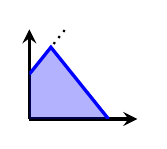
\begin{tikzpicture}[
                baseline={([yshift=-5pt]current bounding box.center)},
                vertex/.style={anchor=base,
                circle,fill=black!25,minimum size=18pt,inner sep=2pt},
                scale=.2]
                \begin{axis}
                [xmin=0, xmax=5,
                ymin=0, ymax=5,
                axis line style = very thick,
                axis y line*=left,
                axis x line*=bottom,
                axis lines = middle,
                ticks=none]
                    \addplot[domain=0:5.0,
                    style=thick,dotted]
                    {2.5 + 1.5*x};
                    \addplot[name path=f,domain=0:3.0,
                    style=very thick,blue]
                    coordinates {
                        (0,2.5) (1.0,4.0)
                        (3.667, 0)
                    };
                    \path[name path=axis]
                    (axis cs:0,0) -- (axis cs:3.0,0);
                    \addplot [
                        thick,
                        color=blue,
                        fill=blue,
                        fill opacity=0.3
                    ]
                    fill between[
                        of=f and axis
                    ];
                \end{axis}
                \end{tikzpicture}
                ~~
            \Bigg]
            & m^2 < \zcut Q^2
            \,,
            \\
            \exp\Bigg[
                ~-~
                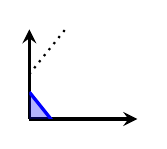
\begin{tikzpicture}[
                baseline={([yshift=8pt]current bounding box.center)},
                vertex/.style={anchor=base,
                circle,fill=black!25,minimum size=18pt,inner sep=2pt},
                scale=.2]
                \begin{axis}
                [xmin=0, xmax=5,
                ymin=0, ymax=5,
                axis line style = very thick,
                axis y line*=left,
                axis x line*=bottom,
                axis lines = middle,
                ticks=none]
                    \addplot[domain=0:5.0,
                    style=thick,dotted]
                    {2.5 + 1.5*x};
                    \addplot[name path=f, domain=0:5,
                    style=very thick, blue]
                    {1.5-1.5*x};
                    \path[name path=axis]
                    (axis cs:0,0) -- (axis cs:1,0);
                    \addplot [
                        thick,
                        color=blue,
                        fill=blue,
                        fill opacity=0.3
                    ]
                    fill between[
                        of=f and axis
                    ];
                \end{axis}
                \end{tikzpicture}
                ~~
            \Bigg]
            &
            m^2 > \zcut Q^2
            \,,
        \end{cases}
    \end{align}
    where the dotted line now indicates \(z = \zcut\theta^{\betasd}\), and has a slope of \(\betasd\).

    If we use only the singular pieces of the splitting functions, integrate \(z\) from 0 to 1 for simplicity/compactness of final results, and keep only leading logarithmic terms in \(\log(m^2/Q^2)\), we obtain the LL result, for a jet initiated by a parton of color representation \(R\),%
    \footnote{
        The result including additional logarithmic terms in \(\zcut\) and non-singular pieces of splitting functions can be found e.g. in \href{https://arxiv.org/pdf/1402.2657\#equation.3.9}{Eq. (3.9)} of \Reff{Larkoski:2014wba} by setting their \(\beta = \betasd\), \(\alpha = 2\).
    }
    %
    \begin{align}
        \label{eq:ll-sd-mass}
        \Sigma^{\rm(LL)}_{m^2}(m^2)
        =
        \begin{cases}
            \exp\le[
                ~-~
                \frac{\alpha_s C_R}{\pi}
                \le(
                    \frac{\betasd \log^2\le(m^2 / Q^2\ri)}
                        {2(2 + \betasd)}
                    +
                    \frac{2 \log(\zcut)\log(m^2/Q^2)}
                        {2 + \beta}
                \ri)
            \ri]
            &
            m^2 < \zcut Q^2
            \,,
            \\
            \exp\le[
                ~-~
                \frac{\alpha_s C_R}{2\pi}
                \,
                \log^2\le(m^2 / Q^2\ri)
            \ri]
            &
            \hspace{-40pt}
            \zcut Q^2 < m^2 < Q^2 / 2
            \,.
        \end{cases}
    \end{align}
\end{example}


\remark{}{
        At LL, strong \gls{angular-ordering} dictates that the \glspl{sub-emission} have angles which are much smaller than \(\thetacrit\), \(\theta_\text{sub} \ll \thetacrit\).
    %
    Therefore, in the LL phase space of pQCD, subsequent emissions are \textit{extremely} unlikely to contribute meaningfully to any additive jet observable (which is the sum of contributions which are monotonic in \(\theta\) and vanish as \(\theta \to 0\)).
    %
    Nonetheless, including the effects of the subsequent emissions on additive observables leads to normalizable resummed distributions for observables whose NLO distributions appear to have singular, non-integrable behavior.
}


\begin{exercise}
    \label{ex:soft-drop-gecf}
    Repeat the analysis of Example \ref{ex:softdrop-mass} to determine the LL distribution of Soft-Drop groomed \textit{angularities} \(e_\varsigma\), when \(\betasd > 0\).
    %
    Compare your answer to the leading-logarithmic terms in \href{https://arxiv.org/pdf/1402.2657#equation.3.9}{Eq. (3.9)} of \Reff{Larkoski:2014wba} after setting their \(\beta = \betasd\), \(\alpha = \varsigma\).
\end{exercise}


\remark{soft-drop-zg}{
    In the context of \gls{soft-drop} \(z_g\) is used to refer to the energy fraction of the first emission to pass the Soft Drop criterion (the \gls{crit-emission}) \(z > \zcut \theta^{\beta_{\rm SD}}\).
    %
    We have already seen the distribution for \(z_g\) in the \gls{constant-cutoff} grooming in \Eq{constant-cutoff-zcrit}, where we called it \(\zcrit\).
    %
    The groomed energy fraction for Soft Drop with \(\betasd = 0\) is identical to that of the constant cutoff algorithm.
    %
    When \(\betasd\neq0\), however, the analysis becomes significantly more complicated.
    %
    Nonetheless, the behavior of \(z_g\) for Soft Drop was derived to double-logarithmic accuracy by \Reff{Larkoski:2015lea} with the technology of Sudakov safety.
    %
    Expanding their double-logarithmic result to \(\mathcal{O}(\alpha_s)\), the \(z_g\) distribution for Soft Drop takes the approximate form
    \begin{align}
        \rho_{i,\,\,\rm SD}(z_g; \beta_{\rm SD}) =
        \begin{dcases}
           \frac{2 \alpha_s C_{R_i}}{\pi |\beta|} \,
           \overline{p}_i(z_g) \,
           \log(z_g /z_c)
           \,
           \Theta(\zcut < z_g)
           +
           \mathcal{O}(\alpha_s^2),
           &
           \beta_{\rm SD} < 0;
           \\
           \frac{\overline{p}_i(z_g)}{\int_{\zcut}^{1/2} \dd z \,\, \overline{p}_i(z)}
           \,
           \Theta(\zcut < z_g),
           &
           \beta_{\rm SD} = 0;
           \\
           \sqrt{\frac{\alpha_s C_{R_i}}{\beta}} \,\, \overline{p}_i(z_g)
           +
           \frac{2 \alpha_s C_{R_i}}{\beta} \,\, \overline{p}_i(z_g)
            \log\min(2\zcut, 2z_g)
           +
           \mathcal{O}(\alpha_s^{3/2}),
           &
           \beta_{\rm SD} > 0,
        \end{dcases}
        \label{eq:sd_zg}
    \end{align}
    where \(i\) again indicates the flavor (quark or gluon) of the initiating parton, and we note that the expression for \(\beta_{\rm SD} = 0\) receives no \(\mathcal{O}(\alpha_s)\) corrections at double-logarithmic accuracy.
    %
    If \(\beta_{\rm SD} \leq 0\), the probability distribution has no support when \(z_g < \zcut\) because \(z_g\) is determined by the Soft Drop criterion;
    %
    the vanishing of the \(z_g\) distribution when \(z_g < \zcut\) for \(\beta_{\rm SD} \leq 0\) therefore reflects the soft discontinuous behavior of Soft Drop.
    %
    If \(\beta_{\rm SD} > 0\) there is instead a kink at \(z_g = \zcut\) that similarly reflects Soft Drop's soft discontinuity.
}


Soft Drop is a conceptually simple, computationally efficient, and theoretically useful tool for understanding the sub-structure of jets.
%
In the next Section, we extend the successes of Soft Drop into the regime of groomers without hard cutoffs, and therefore with better continuity properties.
%
We will introduce a paradigm for continuous jet grooming which, motivated by the geometry of event space, combines techniques from \gls{pu-mitigation} and hard-cutoff grooming.
%
It is the paradigm of \glslink{piranha}{\textbf{P}ileup and \textbf{I}nfrared \textbf{R}adiation \textbf{A}n\textbf{N}i\textbf{H}il\textbf{A}tion} (\textsc{Piranha}) for continuous jet grooming.
%
The name evokes the physical properties of \textsc{Piranha} groomers, which may be thought of as optimal transport algorithms which assign hungry crews of cleanup fish to eat up low-energy pollution within jets.
%
We will find that the \textsc{Piranha} paradigm itself has intricate theoretical properties and several phenomenological advantages.



%==============================================
\section[\textbf{P}ileup and \textbf{I}nfrared \textbf{R}adiation \textbf{A}n\textbf{n}i\textbf{h}il\textbf{a}tion (\textsc{Piranha}):\\A Paradigm for Continuous Jet Grooming]{\textbf{P}ileup and \textbf{I}nfrared \textbf{R}adiation \textbf{A}n\textbf{n}i\textbf{h}il\textbf{a}tion (PIRANHA):\\A Paradigm for Continuous Jet Grooming}
%==============================================
\label{sec:piranha}
\markright{\thechapter.\thesection{} \textsc{Piranha}: A Paradigm for Continuous Jet Grooming}


Popular jet grooming algorithms are soft discontinuous because they introduce hard cutoffs on the energy of jet constituents, removing particles that are too low-energy to be classified as important probes of hard physics.
%
In the constant cutoff algorithm of \Sec{constant-cutoff}, for example, if a soft branch of the \glslink{reclustering}{reclustered} jet tree has an energy fraction \(z = \zcut\), it is kept as a part of the groomed jet.
%
The instant any low-energy pollution pushes its energy to an infinitesimally lower value \(z < \zcut\), however, the soft branch is completely and mercilessly removed from the jet.

Soft discontinuous jet grooming algorithms seem against the spirit of \gls{lphd};
%
we would like the partonic degrees of freedom we attempt to access with jet grooming to be continuously related to the hadronic degrees of freedom of final-state jets.

However, the soft discontinuous behavior of hard-cutoff groomers is not merely an academic concern:
%
it leads to concrete experimental and theoretical complications.
%
Experimentally, discontinuities in grooming can lead to large responses of groomed jet substructure to the interactions of jets with experimental detectors, and therefore to difficulties in unfolding experimental measurements \cite{ATL-PHYS-PUB-2019-027,Aad:2019vyi,ATLAS:2020gwe}.
%
Theoretically, discontinuities in grooming lead to uncertainties in fixed-order calculations \cite{Larkoski:2014wba} -- as mentioned briefly in Remark \ref{rem:cc-discontinuity} -- and even in complications in theoretical descriptions of \gls{hadronization} effects on groomed jet substructure \cite{Hoang:2019ceu}.
%
These complications lead to additional uncertainties when extracting physical parameters, such as the top quark mass, from measurements of jet substructure.
%
This is one reason why recent work in jet substructure is moving instead towards using energy correlators (see \Chap{ewocs}) to extract the top mass \cite{Procura:2022fid,Holguin:2022epo,Holguin:2023bjf,Pathak:2023tmy,Xiao:2024rol,Holguin:2024tkz}.


In this section, we introduce the \PIRANHA{} paradigm for continuous jet grooming.
%
Rather than using hard cutoffs to remove soft radiation from jets, \PIRANHA{} algorithms are \textit{subtractive}, allowing them to remove low-energy pollution from jets \textit{without soft discontinuities}.
%
We begin with a discussion of tree-based \PIRANHA{} algorithms before moving towards more general algorithms which are closely connected to existing techniques for \gls{pileup} mitigation.
%
We discuss how the \PIRANHA{} paradigm applies intuition from optimal transport and recent geometric perspectives in collider physics -- unified by the Energy Mover's Distance (EMD) between collider events~\cite{Komiske:2019fks,Komiske:2020qhg}, reviewed in \Sec{emd} -- to overcome the soft discontinuities of existing jet grooming algorithms.

We begin with a toy example of a \PIRANHA{} groomer in \Sec{constant-cutoff} -- the constant subtraction algorithm, similar to the constant cutoff algorithm of \Sec{constant-cutoff} -- before introducing the three concrete implementations of \PIRANHA{} discussed in this thesis:%
\footnote{
    Code for these three \PIRANHA{} groomers is available on GitHub \cite{piranhagithub}.
    %
    We delegate discussions of \PIRANHA{} grooming in EMD mode to \App{grooming_in_emd_mode}.
}
\begin{itemize}
    \item
        \vocab{\gls{rs}} is a family of nearly-continuous, computationally efficient, tree-based algorithms introduced in \Reff{Alipour-Fard:2023prj}.
    %
    We develop the concrete implementation of \vocab{\glslink{rsf}{Recursive Subtraction with a Fraction \(f_\text{soft}\) (P-RSF\(_{f}\))}} in \Sec{recursive-subtraction}.
    %
    We discuss how P-RSF\(_f\) is discontinuous in suppressed regions of parameter space, and focus on \PRSF{1/2}, which is the only fully soft-continuous version of P-RSF\(_f\);

    \item
    \vocab{\gls{apollonius}}, reviewed in \Sec{fully-continuous-piranha} and originally introduced in \Reff{Komiske:2020qhg}, is a continuous, conceptually simple application of the \PIRANHA{} paradigm with a computationally expensive implementation;

    \item
        \vocab{\gls{ivs}}, also reviewed in \Sec{fully-continuous-piranha} and introduced in \Reff{Komiske:2020qhg}, is a continuous, computationally efficient modification of \gls{apollonius} with a simple geometric implementation.
\end{itemize}



Before we give a more detailed account of \PIRANHA{} grooming, however, let us start with some guiding philosophy.
%
Given a measured collider event \(\mathcal{E}_0\) and a model \(\rhoC\) for the energy density of low energy pollution, we roughly want to subtract out the contamination to obtain a groomed collider event \(\mathcal{E}_g\);
%
na\"ively, we wish to write, formally,
\begin{align}
    \label{eq:naive-subtraction}
    \mathcal{E}_g[\mathcal{E}_0]
    =
    \mathcal{E}_0
    -
    \rhoC
    \,.
\end{align}
However, strict point-wise subtraction (i.e. \(\mathcal{E}_g(\hat{n}) = \mathcal{E}_0(\hat{n}) -\rhoC(\hat{n})\)) is not available to us if we want \(\mathcal{E}_g\) to be a well-defined energy flow:
%
subtraction can produce negative numbers, and negative energies are not allowed in the space of energy flows.
%
However, based on the motivation above, we want a grooming algorithm that behaves \emph{roughly} through subtraction.
%
This motivation will push us to define the constant subtraction and Recursive Subtraction algorithms of \Secs{constant-subtraction}{recursive-subtraction}.

In \Sec{emd}, however, we will introduce technology that will allow us to go further and take \Eq{naive-subtraction} nearly literally.
%
In particular, we will introduce the EMD:
%
a \emph{metric} that enables us to generalize the notion of subtraction.
%
Replacing \(\mathcal{E}\) by \(E\) and \(\rhoC\) by \(c\) for subtraction on the real line, we can write \(E_0 - c = \text{argmin}_{E_g'}d(E_g' + c, E_0)\), where \(d(\cdot,\cdot)\) is the standard metric on the real line.
%
This complicated way of writing regular subtraction of real numbers gives us the correct intuition for how to proceed with the EMD:
%
given an ungroomed event with energy density \(\mathcal{E}_{0}\) in the pseudorapidity-azimuth angle plane and any ansatz \(\rhoC\) for the energy density of low-energy pollution, one particularly succinct \PIRANHA{} algorithm is
%
\begin{align}
    \mathcal{E}_g\left[\mathcal{E}_0\right]
    =
    \underset{\mathcal{E}'}{\arg \min}\ {\rm EMD}_{\beta, R}
    \left(\mathcal{E}_0, \mathcal{E}' + \rhoC\right)
    \label{eq:simple_piranha_intro}
    \,,
\end{align}
where explicit dependent on the EMD metric makes the continuity of \(\mathcal{E}_g\left[\mathcal{E}_0\right]\) manifest.
%
Because the EMD is an optimal transport algorithm, \PIRANHA{} groomers may be roughly imagined as optimally transporting hungry piranhas to eat up delicious low-energy pollution.

\gls{apollonius} is a direct, continuous application of \Eq{simple_piranha_intro} with \(\beta = 1\), and for which \(\rhoC\) is uniform in the pseudorapidity-azimuth plane to approximate common sources of \gls{additive-contamination} such as \gls{pileup} and \gls{ue} \cite{Soyez:2018opl,Monk:2018clo,Sjostrand:1987su,Sjostrand:2014zea,Dasgupta:2007wa,Kirchgaesser:2020poq,Moraes:2007rq,CDF:2015txs,Larkoski:2021hee,Baron:2020xoi,Marzani:2017kqd}.
%
\gls{ivs} approximates \gls{apollonius} and preserves its continuity.
%
Finally, the \glslink{rsf}{Recursive Subtraction with a Fraction 1/2 (\PRSF{1/2})} algorithm we introduce in \Sec{recursive-subtraction} furnishes, to our knowledge, the first example of a soft continuous tree-based jet grooming algorithm;
%
the soft discontinuities of other P-RS algorithms occur only in highly suppressed regions of phase space.


This section is devoted to an introduction of the \PIRANHA{} paradigm.
%
Readers looking for a more detailed discussion of continuity may want to skip to \Sec{discontinuity}, which examines the soft discontinuities present in hard-cutoff groomers and \gls{rsf}, the soft continuity of \PRSF{1/2}, and angular discontinuity in tree-based groomers.


\remark{}{
    Our presentation, beginning with the constant subtraction and P-RS algorithms \emph{before} introducing \gls{apollonius}, is chronologically backwards and chosen with the goal of pedagogical clarity.
    %
    \gls{apollonius} and \gls{ivs} were both introduced in \Reff{Komiske:2020qhg}, and myself and my collaborators introduced P-RS and the \PIRANHA{} paradigm in the follow-up work of \Reff{Alipour-Fard:2023prj}.
    %
    The constant subtraction algorithm that we begin with now is not really of formal interest because it is collinear unsafe;
    %
    however, it exposits the basics of subtractive algorithms without too many algorithmic steps, and is conceptually similar to the constant cutoff algorithm we introduced in \Sec{constant-cutoff}.
    %
    For this reason, we now use the constant subtraction algorithm to introduce the basics of our calculations of \PIRANHA{}-groomed substructure.
}



%=====================================
% RSF Intro
%=====================================
\subsection[Constant Subtraction: A Sneak Peek of \textsc{Piranha} Grooming]{Constant Subtraction: A Sneak Peek of PIRANHA Grooming}
\label{sec:constant-subtraction}


Hard cutoff grooming led to discontinuous behavior because they treat branches of the jet differently when they lie below or above a hard cutoff.
%
When we designed the constant cutoff algorithm in \Sec{constant-cutoff}, for example, we threw away softer branches of the jet when they had an energy fraction \(z < \zcut\).
%
To overcome this difficulty, we will treat particles the same whether they are below or above the cutoff.
%
In this section, we introduce the \emph{constant subtraction} algorithm, which is nearly identical to the constant cutoff algorithm except that it \textit{always} subtracts from the hard branch of the jet by taking \(z \mapsto z_g = z - \zcut\).

The constant subtraction algorithm is not quite a \PIRANHA{} algorithm -- it is not even collinear safe;
%
nonetheless, additive substructure observables computed on constant-subtraction groomed jets \textit{are} collinear safe, and the computation of additive observables in the simple context of this section will give us a sneak peak of computations of jet substructure in the Recursive Subtraction algorithms we explore in \Sec{recursive-subtraction}.

\begin{definitionbox}{Constant Subtraction Grooming Algorithm}{}
    The \vocab{constant subtraction grooming algorithm} is a map which takes in a jet and returns a groomed result.
    %
    It depends on a single parameter \(\zcut \in (0, 1/2)\).
    %
    The constant subtraction algorithm acts on a jet via the following procedure:
    \begin{enumerate}
        \item
            Re-cluster the jet using the angular-ordered C/A algorithm, as discussed in \Sec{reclustering}, and begin \gls{declustering} the jet tree, starting at the base;

        \item
            If the current branch is a final state particle and cannot be \glslink{declustering}{de-clustered}, stop the algorithm;
            %
            otherwise \glslink{declustering}{de-cluster} the current branch into a softer emission with energy fraction \(z\) of the current branch, and a harder emission with energy fraction \(1-z\);

        \item
            If \(z < \zcut\), remove the softer branch from the jet and continue the algorithm recursively by \gls{declustering} the harder branch as in Step 2;

        \item
            Otherwise, if \(z \geq \zcut\), rescale the momenta of all particles in the softer branch by a factor of \((z-\zcut)/z\) (such that the energy fraction of the groomed softer branch relative to its ungroomed parent branch is \(E_{\text{soft, }g}/E_{\text{tot, }0} = z - \zcut\)).
            %
            Continue the algorithm recursively by \gls{declustering} both the softer and the harder branch as in Step 2.
    \end{enumerate}
\end{definitionbox}

Though the constant subtraction algorithm is not technically a \PIRANHA{} algorithm, we are starting to see why the name \PIRANHA{} is suitable;
%
not only does this algorithm annihilate the soft particles associated with \glslink{pileup}{pileup} and infra-red radiation, but it also can be imagined as putting a fish on each softer branch with a hunger for energy (fraction) given by \zcut, and which will subtract from its assigned branch until either it eats its fill or it completely annihilates its meal.


\begin{example}
    In this chapter, we will often compare the substructure of traditionally- and \PIRANHA{}-groomed jets through the behavior of the \gls{gecf} substructure observabes.
    %
    For constant-subtraction-groomed jets, the groomed \gls{gecf} takes the form
\begin{equation}
    \label{eq:subtracted-ecf-defn}
    C_{1,\,g}^{(\varsigma)}(z,\theta)
    =
    \left(z - \zcut\right) \left(\frac{\theta}{R_0}\right)^\varsigma \frac{\left(1 - z\right)}{\left(1 - \zcut\right)^2}
    \approx
    \left(z - \zcut\right)\left(\frac{\theta}{R_0}\right)^\varsigma
    \,,
\end{equation}
up to subleading terms in \(\zcut\) that we ignore.
\end{example}


\begin{example}
    \label{ex:constant-subtraction-gecf}
    As usual when studying additive substructure observables, we will use the reduced splitting functions \(\bar{p}(z) = p(z) + p(1-z)\), \(z \in (0,1/2)\), since the \(C_{1,\,g}^{(\varsigma)}\) are sensitive to the softest emission in the jet.
    %
   The fixed-order distribution of \(C_{1,\,g}^{(\varsigma)}\) away from zero becomes
%
\begin{align}
    \rho^{\rm(NLO)}_{i,~\varsigma}(C>0)
    =
    \frac{\alpha_s}{\pi}\int_0^{R_0}\frac{\dd\theta}{\theta}
    \int_0^{1/2} \dd z\, \Bar{p}_i(z)
    \delta\left(C - C_{1,\,g}^{(\varsigma)}(z,\theta)\right),
    \label{eq:NLO_dist_setup}
\end{align}
%
where  \(C_1^{(\varsigma)}(z,\theta)\) is the functional form of the groomed ECF given in \Eq{subtracted-ecf-defn}.

Up to terms that are power-suppressed in \(C\), \(\zcut\), or both, the fixed-order distribution for the groomed observable away from \(C = 0\) is
%
\begin{subequations}
\label{eq:piranha_nlo}
\begin{align}
    \rho^{\rm(NLO)}_{i,~\varsigma}(C>0)
    &=
    \frac{2\alpha_s C_{R_i}}{\varsigma~\pi}
    \frac{1}{C}
    \left(
        2\tanh^{-1}\left(1  -2 \tilde C - 2\zcut\right)
        + B_i
        +
        \mathcal{O}\left(C,\,\zcut\right)
    \right)
    \\
    &=
    \frac{2\alpha_s C_{R_i}}{\varsigma~\pi}
    \frac{1}{C}
    \left(
        -\log\left(\tilde C + \zcut\right)
        + B_i
        +
        \mathcal{O}\left(C,\,\zcut\right)
    \right)
\end{align}
\end{subequations}
%
where \(\tilde C = C \times (1-\zcut)^2\), \(C_{R_i}\) is the quadratic Casimir of the color representation of the initiating parton, and we have defined the factor \(B_i\) to capture behavior from non-singular components of the splitting functions:
%
\(B_q = -3/4\) for quark initiated jets and \(B_g = -11/12 + N_f/(6 C_A)\) for gluon initiated jets.
\end{example}

\begin{exercise}
    \label{ex:constant-subtraction-virtual}
    Argue that including the \(\mathcal{O}(\alpha_s^0)\) jet configuration with a single parton for which \(C_1^{(\varsigma)} = 0\), the two-parton contributions for which \(z < \zcut\) and the softer emission is completely eliminated, and the virtual contributions at \(\mathcal{O}(\alpha_s^1)\), we can write the full \glslink{accuracy}{NLO} probability distribution for \(C_1^{(\varsigma)}\) as
\begin{align}
    \label{eq:plusdist_prsf_nlo}
    \rho^{\rm(NLO)}_{i,~\varsigma}(C)
    &\approx
    \delta(C)
    +
    \frac{2\alpha_s C_{R_i}}{\varsigma~\pi}
    \left[\frac{1}{C}
    \left(
        -\log\left(\tilde C + \zcut\right)
        + B_i
        +
        \mathcal{O}\left(C,\,\zcut\right)
    \right)
    \right]^{(C_{\rm max})}_+
    ,
\end{align}
where \({C_{\rm max}} = (1 - \zcut)^{2}/4\) is the maximum possible value of \(C_1^{(\varsigma)}\) (achieved when \(z = (1+\zcut)/2\)), and the normalization of the distribution is fixed with \glslink{plus-fn}{plus-function regularization}.

\vspace{10pt}
\hrule

\vspace{-3pt}

\begin{center}
\texttt{(Hint:)}
\end{center}

\vspace{-3pt}

\noindent
The plus-function regularized expression of \Eq{plusdist_prsf_nlo} may be derived by replacing \(\overline{p}(z)\) in \Eq{NLO_dist_setup} with its plus-function analog.
%
Alternatively, one can recognize that the full distribution for \(C_1^{(\varsigma)}\) must integrate to one even at \glslink{accuracy}{NLO}, and that additional contributions to the \glslink{accuracy}{NLO} distribution in \Eq{prsf_NLO} can only come from the regions of phase space where \(C_1^{(\varsigma)}=0\);
%
this \gls{sum-rule} is enough to uniquely specify the result of \Eq{plusdist_prsf_lo} at \glslink{accuracy}{NLO}.
\end{exercise}



\remark{}{
    Since \PIRANHA{} algorithms are subtractive, and subtraction from the harder branch of an emission has a subleading effect on the value of \(C_1^{(\varsigma)}\), \Eq{plusdist_prsf_nlo} provides an approximate expression for the NLO distribution of \(C_1^{(\varsigma)}\) for any \PIRANHA{}-groomed jet.
    %
    Though the value of the effective grooming parameter may depend on the configuration of the particles for a more generic \PIRANHA{} groomer -- i.e. though in principle we must replace \(\zcut\to \zcut(z,\theta)\) -- we may use the soft and collinear limits to justify replacing \(\zcut(z,\theta)\) by \(\zcut(0,0)\) in \Eq{plusdist_prsf_nlo} for the applications considered in this thesis.
    %
    We can do even better by subtracting from both the hard and the soft branches, as we discuss in \Sec{pira-resummed} when performing calculations of \glspl{gecf} for jets groomed with \glslink{rs}{Recursive Subtraction (P-RS)}.
}

\remark{}{
    Unlike the \glslink{accuracy}{NLO} distributions for traditionally groomed jet ECFs, such as those of Soft Drop \cite{Larkoski:2014wba}, the \glslink{accuracy}{NLO} distributions for \PRSF{1/2} and \gls{rsf} groomed \(C_1^{(\varsigma)}\) do not exhibit piece-wise behavior.
    %
    While the piece-wise behavior of Soft Drop observable distributions is smoothed out by all-orders effects \cite{Benkendorfer:2021unv}, the smoothness of \PIRANHA{}-groomed distributions at \glslink{accuracy}{NLO} is a manifestation of their continuity.
}


\begin{exercise}
    Show that the \glslink{accuracy}{LL} radiator for the constant-subtraction-groomed \gls{gecf}, not including running coupling effects and ignoring subleading effects in \zcut, can be captured by the globally-defined function
    \begin{align}
        R^{\text{(NLO)}}_\varsigma(C)
        \approx
        \frac{2\alpha_s C_{R_i}}{\varsigma~\pi}
        \Bigg(
            &
            -\text{Li}_2\le(-\frac{(1-\zcut)^2}{\zcut} C\ri)
            +
            \le(\log(\zcut) + B_i\ri)\log(C)
            \\
            &
            \notag
            +
            \text{Li}_2\le(-\frac{(1-\zcut)^4}{4\zcut}\ri)
            -
            \le(\log(\zcut) + B_i\ri)
            \log\le(\frac{(1-\zcut)^2}{4}\ri)
        \Bigg)
        \,.
    \end{align}

    Argue that we can use \Eq{resummed-multiple-emissions} to realize a well-defined, continuous probability distribution for the constant-subtraction-groomed \gls{gecf} which includes the effects of multiple emissions.
\end{exercise}



%=====================================
% The PIRANHA Paradigm for Jet Grooming:
%=====================================
\subsection{Recursive Subtraction (P-RS)}
\label{sec:recursive-subtraction}
% \label{sec:rsf}

\gls{rs} is a further extension of the \PIRANHA{} paradigm into the space of tree-based grooming algorithms based on \gls{declustering}.
%
We use ``Recursive Subtraction'' to denote an algorithm that takes in a binary tree of emissions describing a jet and recursively subtracts from the momenta of its jet constituents.
%
\gls{rs} was the original tree-based \PIRANHA{} groomer, and was motivated by the area-based subtraction techniques of \gls{apollonius} and \gls{ivs} -- which leverage a connection to optimal transport and geometry to obtain the advantage of continuity -- but borrows from the computational efficiency and connection to \gls{pqcd} of tree-based hard-cutoff groomers.
%
By combining these strengths, \gls{rs} paves the way for \PIRANHA{} groomers that are experimentally useful and theoretically tractable.


\begin{definitionbox}{}{}
    \gls{rs} refers to any \gls{declustering}-based grooming algorithm, based on the subtraction principle of \PIRANHA{}, which takes in a total amount of transverse momenta to subtract from the clustered jet
    %
    At each splitting in the tree, \gls{rs} assigns a fraction of the total grooming assigned to the current branch to the softer emission associated with the splitting, and the remaining grooming to the harder emission.
    %
    When the \gls{declustering} finally reaches the final-state particles of a jet, P-RS subtracts directly from their transverse momenta.
\end{definitionbox}


The simplest family of \gls{rs} algorithms are the \glslink{rsf}{Recursive Subtraction with a Fraction (P-RSF)} algorithms, which always assign the same fraction \(f\) of grooming to the softer branch of the jet tree:



\begin{definitionbox}{Recursive Subtraction with a Fraction \(f_{\rm soft}\) (P-RSF)}{rsf}
    \vocab{Recursive Subtraction with a Fraction \(\boldsymbol{f}_{\rm\bf soft}\)} (P-RSF\(_f\), or \gls{rsf}) is a simple implementation of P-RS that does not depend on the kinematic information of each splitting.
    %
    \gls{rsf} depends on two real parameters:
    %
    \begin{itemize}
        \item
        \(\zcut\), between 0 and 1/2, is the fraction of transverse momentum the grooming will remove from the entire jet, \(p_{T,\,\text{P-RSF}} = (1 - \zcut) p_{T,\,\rm tot}\).
        %
        We may write \(\zcut = \zcut^{(0)} = \rho A_{\rm jet} / p_{T,\,\rm jet}\), which will be analogous to the ``piranha energy density'' \(\rho\) of \gls{apollonius} and \gls{ivs} discussed in \Sec{fully-continuous-piranha}.
        %
        We denote the total transverse momentum removed from the jet as \(\Delta^{(0)} = \zcut\,p_{T,\,\rm tot}\), and the transverse momentum removed from a branch \(i\) of the jet is \(\Delta^{(i)} = \zcut^{(i)}\,p_{T,\,\rm tot}\);

        \item
        \(f_{\rm soft}\), between 0 and 1, is the fraction of the grooming assigned to the softer sub-jet at each stage of the \gls{declustering}, as detailed below.
        %
        \gls{rsf} prefers to groom softer radiation more and more as \(f_{\rm soft}\) increases.
    \end{itemize}


    \vspace{7pt}
    \hrule
    \vspace{7pt}

    In the steps of the algorithm below, we index the current branch of the jet on which P-RSF is acting by \(i\).
    %
    The softer sub-jet of branch \(i\) is denoted ``\(i,\,\text{soft}\)'', and the harder branch is denoted ``\(i,\,\text{hard}\)''.
    %
    If the algorithm is at its starting point and considering the entire jet, we write \(i = 0\).

    The concrete prescription of \gls{rsf} is as follows:
    \begin{enumerate}
        \item
        \gls{rsf} attempts to \glslink{declustering}{de-cluster} sub-jet \(i\) into two sub-jets.
        %
        If this is impossible, the branch corresponds to a final-state particle and \gls{rsf} proceeds to Step 5.
        \label{item:rsf_initial}

        \item
        \gls{rsf} divides the grooming assigned to branch \(i\) between the softer sub-jet (\(i,\,\text{soft}\)) and the harder sub-jet (\(i,\,\text{hard}\)):
        \begin{align}
            \Delta^{(i,\,\text{soft})}
        &=
        f_{\rm soft} \, \Delta^{(i)}
        \overset{\Delta}{=}
        \zcut^{(i,\,\text{soft})} p_{T,\, \rm tot}
        \\
            \Delta^{(i,\,\text{hard})}
        &=
        (1-f_{\rm soft}) \, \Delta^{(i)}
        \overset{\Delta}{=}
        \zcut^{(i,\,\text{hard})} p_{T,\, \rm tot}
            ,
        \end{align}
        so that \(\Delta^{(i,\,\text{soft})} + \Delta^{(i,\,\text{hard})} = \Delta^{(i)}\).
        %
        In words, \gls{rsf} assigns a fraction \(f_{\rm soft}\) of the grooming to the softer sub-jet, and the remaining fraction \(1 - f_{\rm soft}\) to the harder sub-jet.
        %
        Equivalently,
        \begin{align}
            \zcut^{(i,\,\text{soft})} &= f_{\rm soft} \zcut^{(i)}
            \\
            \zcut^{(i,\,\text{hard})} &= (1-f_{\rm soft}) \zcut^{(i)}
            ,
        \end{align}
        so that \(\zcut^{(i,\,\text{soft})} + \zcut^{(i,\,\text{hard})} = \zcut^{(i)}\).
        \label{item:rsf_softhard}

        \item
        \gls{rsf} checks if one of the sub-jets of the current branch is removed by the grooming:

        \begin{enumerate}
        \item
        If the grooming assigned to the softer sub-jet is greater than its actual transverse momentum, \(\Delta^{(i,\,\text{soft})} > p_T^{(\rm i,\,\text{soft})}\), \gls{rsf} removes the softer sub-jet from the event.
        %
        \gls{rsf} then assigns the remaining grooming to the harder sub-jet, \(\Delta^{(i,\,\text{hard})} = \Delta^{(i)} - p_T^{(\rm i,\,\text{soft})}\).
        \label{item:remove_soft}

        \item
        Similarly, if the grooming assigned to the harder sub-jet is greater than its transverse momentum, \(\Delta^{(i,\,\text{hard})} > p_T^{(\rm i,\,\text{hard})}\), \gls{rsf} removes the harder sub-jet from the event.
        %
        It then assigns the remaining grooming to the softer sub-jet, \(\Delta^{(i,\,\text{soft})} = \Delta^{(i)} - p_{T}^{(i,\,\text{hard})}\).
        %
        This is possible only if \(f_{\rm soft} < 1/2\).
        \label{item:remove_hard}
        \end{enumerate}

        \item
        \gls{rsf} implements Step~\ref{item:rsf_initial} on the surviving sub-jets of \(i\) using the values of \(\Delta^{(i,\,\text{soft})}\) and \(\Delta^{(i,\,\text{hard})}\) calculated in the previous two steps.

        \item
        When \gls{rsf} reaches a final-state particle (a branch that cannot be further divided), it subtracts the grooming from its transverse momentum, effectively adjusting its energy fraction.
        %
        Explicitly,
        \begin{align}
            p^{(i)}_{T,~{\rm P-RSF}} = p^{(i)}_T - \Delta^{(i)}.
        \end{align}
        Here, \(p^{(i)}_{T,~{\rm P-RSF}}\) denotes the groomed \(p_T\) of the final-state particle associated with the current branch \(i\).
        %
        This may also be described as a shift in the fraction of the total transverse momentum carried by the particle \(i\),
        \begin{align}
            z^{(i)}_{\text{P-RSF}} = (z^{(i)} - \zcut^{(i)})/(1-\zcut)
            ,
        \end{align}
        where the additional factor of \(1 - \zcut\) is due to normalization to the groomed transverse momentum.
        \label{item:rsf_final}
    \end{enumerate}
\end{definitionbox}

\gls{rsf} builds on the strengths of the P-RS framework, providing a simple implementation that does not rely on detailed kinematic information.
%
By combining the advantages of tree-based hard-cutoff and continuous \PIRANHA{} grooming paradigms, \gls{rs} and \gls{rsf} offer a promising path for experimentally useful and theoretically tractable continuous groomers.
%
A visualization of \gls{rsf} acting on a tree of emissions for \(f_{\rm soft} = 1/2\) (which we also call \vocab{Balanced P-RSF}) and \(f_{\rm soft} = 1\) (an example of \gls{rsf}\(_{f_{\rm soft}\neq1/2}\) or \vocab{Unbalanced P-RSF}) is shown in \Fig{rsf_tree}.


%-----------------------------------
% \PRSF{1/2} Tree fig.:
%-----------------------------------
\begin{figure}[t!]
      \centering
      \centerline{
      \subfloat[]{
      \begin{tikzpicture}
          \node at (0,0) {
              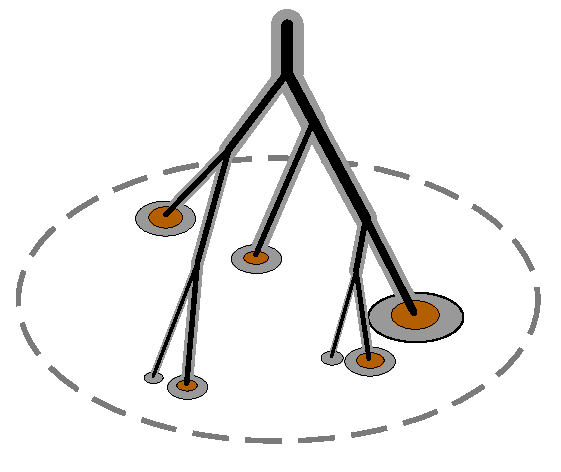
\includegraphics[width=.4\textwidth]{figures/piranha/cartoons/RSF_half_vis.pdf}
          };
          % \node at (0, 3.3) {Visualization of \normalsize \PRSF{1/2} (Balanced P-RSF)};
          % \node at (0, 2.8) {acting on a toy event};
          \node at (0, 2.8) {\normalsize \PRSF{1/2} (Balanced P-RSF)};
      \end{tikzpicture}
      \label{fig:rsf_half_vis}
      }
      ~~~~
      \subfloat[]{
      \begin{tikzpicture}
          \node at (0,0) {
              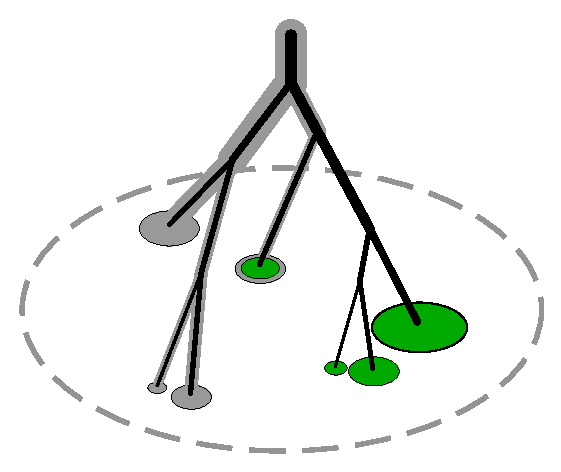
\includegraphics[width=.4\textwidth]{figures/piranha/cartoons/RSF_1_vis.pdf}
          };
          % \node at (0, 3.3) {Visualization of \normalsize \PRSF{1} (an example of};
          % \node at (0, 2.8) {Unbalanced P-RSF) acting on a toy event};
          \node at (0, 2.8) {\normalsize \PRSF{1} (example of Unbalanced P-RSF)};
      \end{tikzpicture}
      \label{fig:rsf_1_vis}
      }
      } % centerline
      \caption[Visualizations of recursive subtraction algorithms acting on toy jets.]{
    Visualization of (a) \PRSF{1/2} and (b) \PRSF{1} acting on a toy jet depicted as an angular-ordered tree of emissions.
    %
    The jet cone is indicated by the dashed ellipse, and the groomed final-state particles are indicated by colored ellipses, in dark orange (\PRSF{1/2}) and green (\PRSF{1});
    %
    the size of each circle is proportional to the groomed \(p_T\) of the corresponding particle.
    %
    The grey highlights behind each emission in the tree indicate the transverse momentum subtracted from each branch, and eventually from the final-state particles of that branch, as described in \Sec{recursive-subtraction}.
    %
    The size of the grey highlights behind each final-state particle indicates the amount of transverse momentum subtracted from that particle.
}
\label{fig:rsf_tree}
\end{figure}



%=====================================
% Continuity of P-RSF:
%=====================================
\gls{rsf} is well-defined on the space of energy distributions of particle events because it is invariant under exactly collinear splittings.
%
To see this, we first notice that exact collinear splittings are infinitely narrow, and always correspond to branchings at the final layer of an angular-ordered tree of emissions.
%
With this in mind, let us implement an exact collinear splitting, replacing a final-state particle \(i\) within a jet by two exactly collinear final-state particles, ``\(i,\,\text{soft}\)'' and ``\(i,\,\text{hard}\)''.
%
Following the presentation of \Sec{recursive-subtraction}, the transverse momentum subtracted from the new final state particles adds up to the transverse momentum subtracted from \(i\), \(\Delta^{(i,\,\text{soft})} + \Delta^{(i,\,\text{hard})} = \Delta^{(i)}\).
%
Since \(i,\,\text{soft}\) and \(i,\,\text{hard}\) are exactly collinear, the energy distribution of \(i\) after grooming is equal to the sum of the energy distributions for \(i,\,\text{soft}\) and \(i,\,\text{hard}\) after grooming.
%
The result of the \gls{rsf} grooming procedure is therefore robust against exactly collinear splittings for any value of \(f_{\rm soft}\).

While the subtractive algorithm of \gls{rsf} cannot be expressed simply in terms of geometry, \gls{rsf} echoes the features of \gls{apollonius} and \gls{ivs} that grant their continuity.
%
For example, Steps 3(a) and 3(b)
%Steps~\ref{item:remove_soft} and~\ref{item:remove_hard}
of the \gls{rsf} algorithm ensure that \gls{rsf} does not assign an area to any final-state particle that is larger than its transverse momentum.

However, \gls{rsf} still suffers from discontinuities in suppressed regions of parameter space.
%
We show in \Sec{rsf_discont} that Unbalanced \gls{rsf}, or \gls{rsf} with \(f_{\rm soft} \neq 1/2\), suffers from soft discontinuities:
%
small changes to the energy of the jet have the potential to change which emissions of the jet are softer.
%
The balanced recursive subtraction procedure, \PRSF{1/2}, overcomes this weakness and is soft-continuous.
%
Furthermore, \Sec{ang_discont} discusses how recursive tree-based grooming algorithms suffer from discontinuities inherited from pairwise clustering, leading to angular discontinuities in both Balanced and Unbalanced \gls{rsf} as well as traditional grooming algorithms such as Soft Drop.


%=====================================
% EMD:
%=====================================
\subsection{The Energy Mover's Distance and Precise Notions of Continuity}
\label{sec:emd}

We now prepare for a precise definition of continuity, and therefore a precise characterization of the continuity properties of \PIRANHA{} groomers.
%
\Gls{continuity} roughly means that small changes in the input to a function only lead to small changes to the output of the function.
%
Therefore, to define continuity, we will need to define what is meant by a ``small change'' in the final state of a particle collision event.

The tool we will use to understand when two particle collision events are similar is the \textit{Energy Movers' Distance} of Ref.~\cite{Komiske:2019fks}, which provides a quantitative measure of the similarity between two jets.
%
We introduce the EMD here both to facilitate our definition of continuity in jet grooming and as a useful tool for quantifying the responses of jet groomers to low-energy pollution.

%%
%Here and in the remainder of the paper, we borrow the terminology of \Reff{Komiske:2020qhg} and use the terms ``event'' and ``collider event'' to refer to the \textit{energy flow} of the event, or the angular distribution of energy of its outgoing radiation (as in \Def{energy-flow}).



\begin{definitionbox}{Energy Mover's Distance (EMD)}{emd}
    The EMD is a metric on the space of collider events which may be thought of as the amount of ``work'' required to rearrange one event into another.

    \vspace{7pt}
    \hrule
    \vspace{7pt}

    For events that consist of a finite number of outgoing particles, the \vocab{Energy Movers' Distance (EMD)} is defined as the solution to the optimal transport problem
    \begin{equation}
        \label{eq:EMD_def_1}
        {\rm EMD}_{\beta, R}\left(\mathcal{E}, \mathcal{E}'\right)
        =
        \min_{f_{ij} > 0} \sum_{i = 1}^M \sum_{j = 1}^{M'} f_{ij} \left(\frac{\theta_{ij}}{R}\right)^\beta
        +
        \left| \sum_{i = 1}^M E_i -  \sum_{j = 1}^{M'} E'_j\right|,
    \end{equation}
    \begin{equation}
        \sum_{i = 1}^M f_{ij} \leq E_j',
        ~~
        \sum_{j = 1}^{M'} f_{ij} \leq E_i,
        ~~
        \sum_{i = 1}^M \sum_{j = 1}^{M'} f_{ij}
        = \min\left(\sum_{i = 1}^M E_i, \sum_{j = 1}^{M'} E'_j\right)
        \label{eq:EMD_def_2}
        ,
    \end{equation}
    where \(i \in \{1, ..., M\}\) indicates a final-state particle of \(\mathcal{E}\) with energy \(E_i\), \(j \in \{1, ..., M'\}\) indicates a final-state particle of \(\mathcal{E}'\) with energy \(E'_j\), and \(\theta_{ij}\) denotes an angular distance between particles \(i\) and \(j\).
    %
    \(\beta > 0\) and \(R > 0\) are free parameters that control the behavior and relative importance of the first term on the right-hand side of \Eq{EMD_def_1}.\footnote{
    Strictly speaking, the EMD defines a metric only if \(2 R\) is greater than the maximum possible angular distance \(\theta_{ij}\).
    %
    Furthermore, for \(\beta > 1\), one must raise the first term of \Eq{EMD_def_1} to the \(1/\beta\) power.
    %
    We use the EMD without a subscript, \(
    {\rm EMD}\left(\mathcal{E}, \mathcal{E}'\right)
    \) to denote the EMD with \(\beta = 1\) and with large enough \(R\) that it furnishes a metric.
    }
\end{definitionbox}


We adopt the hadronic angular measure of \Reff{Komiske:2020qhg}, given by
\begin{equation}
    \theta_{ij} = \sqrt{-(n_i - n_j)^2}
    ,
    ~~~~~~
    ~~~~~~
    n_{i}^\mu = \frac{p_i^\mu}{E_{T\,i}} = (\cosh(y_i), \textbf{v}_{T\,i}, \sinh(y_i))^\mu
    .
    \label{eq:hadronic_metric}
\end{equation}
Here, \(n_i^\mu\) is a vector describing the motion of particle \(i\), parametrized by its rapidity \(y_i\) and its velocity \(\textbf{v}_{T\, i}\) in the directions transverse to the beampipe.
%
This angular metric reproduces the rapidity-azimuth distance between particles \(i\) and \(j\) in the small rapidity-azimuth distance limit.\footnote{
Another popular choice for the form of the \(n_i^\mu\) is captured by
\begin{align}
    \label{eq:ee_metric}
    n_{i,~{e^+e^-}}^\mu = \frac{p_i^\mu}{E_i} = (1, \textbf{v}_i)^\mu
    ,
\end{align}
which is a natural choice in the study of electron-positron collisions~\cite{Komiske:2020qhg}.
%
This choice reproduces the real-space opening angle between particles \(i\) and \(j\) in the small angle limit.
}

The EMD between a groomed jet in the presence and absence of low-energy pollution also provides an observable-independent tool for quantifying the sensitivity of jet grooming to pollution from \glspl{soft-distortion} and \gls{additive-contamination}.
%
Since the EMD furnishes a metric on the space of events, two events are separated by zero EMD iff they have identical energy flow, and two jets separated by zero EMD will yield the same value for every infra-red/collinear (IRC) safe observable (see \href{https://arxiv.org/pdf/2004.04159.pdf#page=11\&zoom=100,0,650}{Lemma 1} of \Reff{Komiske:2020qhg}).
%
Further, the EMD between two events also \textit{directly} bounds the differences in a large class of IRC-safe observable quantities (Lipschitz continuous observables) between the events~\cite{Komiske:2019fks}.
%
For example, the EMD between a parton-level jet and the same jet after \gls{hadronization} (the parton-hadron EMD) directly bounds the difference between a large class of parton- and hadron-level IRC-safe observables.
%
The parton-hadron EMD is therefore a powerful, observable independent tool for characterizing the response of a jet to \glspl{soft-distortion} from \gls{hadronization}.
%
We use the EMD in our analysis of the sensitivity of grooming to several sources of low-energy pollution in Sections \ref{sec:pira-hadronization} through \ref{sec:pira-ue}.


We may use the EMD to define continuity more precisely for maps on energy flows, in the spirit of \href{https://arxiv.org/pdf/2004.04159.pdf#page=5\&zoom=100,0,350}{Definition 1} of \Reff{Komiske:2020qhg}:
%
\begin{definitionbox}{Continuity at an Event}{eventcontinuity}
    \emph{\glslink{eventcontinuity}{continuous at an event}}

    \vspace{7pt}
    \hrule
    \vspace{7pt}

    A map \(M\) from energy flows to energy flows is \vocab{continuous at an event \(\mathcal E\)} if, for any \(\varepsilon > 0\), there exists a \(\delta > 0\) such that for all \(\mathcal E'\),
    %
    \begin{equation*}\label{eq:emdcontinuity}
        {\rm EMD}(\mathcal E,\mathcal E')<\delta
        \quad\implies\quad
        {\rm EMD}(M(\mathcal E), M(\mathcal E')) < \varepsilon.
    \end{equation*}
    %
    We say that \(M\) is \textbf{continuous} if it is continuous at all events \(\mathcal{E}\).
\end{definitionbox}
%
\noindent Definition~\ref{def:eventcontinuity} encodes the requirement that a continuous grooming algorithm must map jets that are infinitesimally nearby in event space to groomed results that are also infinitesimally close.\footnote{
%Our Definition~\ref{def:eventcontinuity} is in the spirit of \href{https://arxiv.org/pdf/2004.04159.pdf\#page=5\&zoom=100,114,645}{Definition 1} of \Reff{Komiske:2020qhg}.
Equivalently, we may say that a grooming procedure is continuous if it maps nearby jets to nearby groomed jets.
%
An event \(\mathcal{E}\) is \textbf{near} an open ball \(\mathcal{B}\) if any neighborhood of \(\mathcal{E}\) contains events in \(\mathcal{B}\).
%
On the real line, for example, the point \(E = 1\) is near the open ball \(B = (-1, 1)\).
%
A grooming procedure \(G\) is then \textbf{continuous} if for any event \(\mathcal{E}\) and open ball \(\mathcal{B}\),
%\begin{equation*}
    \(
    \mathcal{E} {\text ~is~ near~} \mathcal{B}
    \implies
    G(\mathcal{E}) {\text~ is~ near~} G(\mathcal{B}).
    \)
%\end{equation*}
}
For the more complicated \PIRANHA{} groomers we introduce in this paper, it will be helpful to define two additional properties that are required by full continuity:
\begin{itemize}
    \item
        \glslink{soft-discontinuity}{\vocab{Soft Continuity}} is the requirement that a groomer is invariant under infinitesimally soft perturbations of the energies of jet constituents;

    \item
        \glslink{angular-discontinuity}{\vocab{Angular Continuity}} is the requirement that a groomer is invariant under infinitesimally small angular changes in the directions of jet constituents.
\end{itemize}


We will see that hard-cutoff groomers and even many recursive subtraction algorithms suffer from soft discontinuity in \Secs{softdrop}{rsf_discont} respectively.
%
In \Sec{ang_discont}, we will explore how tree-based grooming algorithms -- hard-cutoff and \PIRANHA{} alike -- may inherit angularly discontinuous behavior from angular-ordered jet clustering.\footnote{
Collinear safety, or invariance under exact collinear splittings which replace a final-state particle of momentum \(p^\mu\) by two particles with momenta \(\lambda p^\mu\) and \((1-\lambda) p^\mu\), is a weaker condition.
%
Exact collinear splittings do not change the energy distribution associated with an event; therefore, any well-defined map on the space of particle events must be collinear safe~\cite{Komiske:2020qhg}.
}



%=====================================
% The PIRANHA Paradigm for Jet Grooming:
%=====================================
\subsection[Back to School: Fully Continuous \textsc{Piranha} Grooming]{Back to School: Fully Continuous PIRANHA Grooming}
\label{sec:fully-continuous-piranha}

\PIRANHA{} grooming may be intuitively imagined as the optimal transport of a group of hungry piranhas towards the low-energy pollution within a jet.
%
In this analogy, henceforth the piranha analogy, a \PIRANHA{} groomer populates the \(\eta\)-\(\phi\) plane with a school of piranhas, distributed according to a particular model of the polluting energy density.
%
When they are given an event to groom, the piranhas discuss which piranhas will get to eat which jet constituent;
%
in the language of optimal transport, we say that the piranhas decide on a set of transport plans.
%
The piranhas then implement the plan and feed on the constituents of the jet, or subtract from the \(p_T\) of each jet constituent.
%
%\PIRANHA{} grooming uses optimal transport to design \textit{continuous} grooming procedures that have reduced sensitivity to low-energy pollution.
%%
%In particular, continuity requires that minuscule changes to the jet do not dramatically change the resulting groomed jet.
%
In the piranha analogy, continuity emerges when the piranhas' transport plans do not respond dramatically to small changes in the constituents of an ungroomed jet.
%
Since both \glspl{soft-distortion} and fluctuations in \gls{additive-contamination} may lead to small changes in an event, continuity helps ensure that neither dramatically changes the information carried by groomed jets.


The EMD itself also furnishes an example of an optimal transport problem, allowing us to immediately introduce a simple, generic \PIRANHA{} groomer.
%
To begin, let us model the radiation that we would like to remove from our jet as a distribution of energy \(\rhoC\) in a portion of the rapidity-azimuth (\(\eta\)-\(\phi\)) plane with area \(A\).
%
We use \(\rho\) to indicate the mean energy density and \(\mathcal{C}\) to indicate a distribution modeling the shape of the contaminating radiation, normalized such that
\begin{equation}
    \rho\int \dd y\,\dd\phi\,\mathcal{C}(y,\phi) = \rho A = E
\end{equation}
gives the total energy of the \gls{additive-contamination} we would like to remove.
%
Again echoing \Reff{Komiske:2020qhg}, we may phrase the subtraction of the energy distribution \(\rhoC\) from an event \(\mathcal{E}\) as the solution to the optimal transport problem
\begin{align}
    \label{eq:simple_piranha}
    \mathcal{E}_g[\mathcal E_0] = \underset{\mathcal{E}'}{\arg \min}\ {\rm EMD}_{\beta, R}
    \left(\mathcal{E}_0, \mathcal{E}' + \rhoC\right)
    .
\end{align}
%
It was shown in \href{https://arxiv.org/pdf/2004.04159.pdf#page=33\&zoom=100,0,0}{Lemma 3} of \Reff{Komiske:2020qhg} that \Eq{simple_piranha} defines a subtractive algorithm that merely decreases the energy of jet constituents, and does not add new particles to an event.
%
In the piranha analogy, \(\rhoC\) roughly describes the distribution of our piranhas, with a ``piranha energy density'' \(\rho\), while the minimization problem of \Eq{simple_piranha} provides them with the transport plans that guide them to subtract from the \(p_T\) of jet constituents.
%
Furthermore, the form of \(\mathcal{E}_g[\mathcal E_0]\) in \Eq{simple_piranha} is manifestly continuous due to its dependence on the EMD metric.


\remark{care-with-continuity}{
    While \(\mathcal{E}_g[\mathcal E_0]\) in \Eq{simple_piranha} is continuous, manifest continuity due to dependence on the EMD should be treated skeptically.
    %
    For example, the ``grooming procedure'' associated with  \Eq{simple_piranha} may not be continuous if the \(\arg \min\) operation is restricted to a non-convex sub-space of the full space of events.
    %
    Analogously, \(
        f(x)
        =
        \underset{y}{\arg \min}\ ||x, y+1||
        =
        x-1
    \)
    is continuous as a map from \(\mathbb R\) to \(\mathbb R\) with the standard topology.
    %
    However, \(
        g(x)
        =
        \underset{y \in \{0, 1\}}{\arg \min}\ ||x, y+1||,
    \)
    which differs only by the allowed values of \(y\) in the \(\arg \min\), is not.
}



%-----------------------------------
% Apollonius fig.:
%-----------------------------------
\begin{figure}[t!]
\centering

\subfloat[%\normalsize Visualizing the \PIRANHA{} Paradigm
]{
\begin{tikzpicture}
\node at (0,0) {
    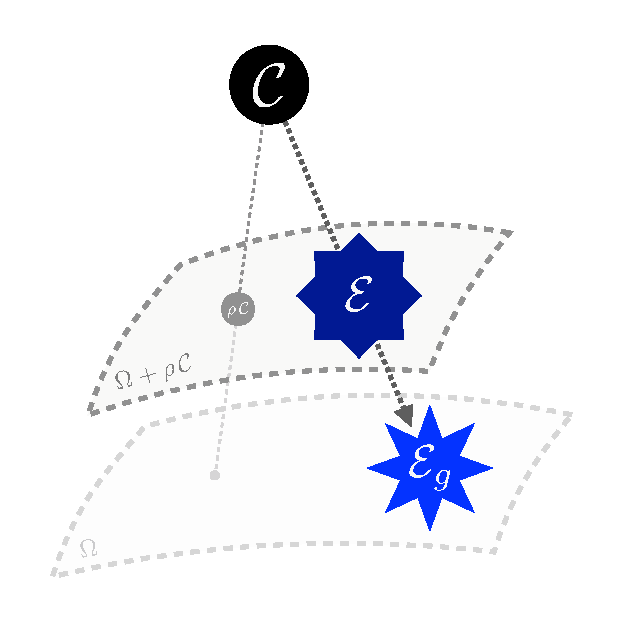
\includegraphics[width=0.45\textwidth]{figures/piranha/cartoons/space_pu}
};
\node at (0,4.25) {Cartoon of a \PIRANHA{} groomer};
\node at (0,3.75) {acting on the space of energy flows};
\end{tikzpicture}
\label{fig:piranha_projection}
}
\subfloat[%\normalsize Apollonius Subtraction
]{
\begin{tikzpicture}
\node at (0,0) {
\includegraphics[width=0.45\textwidth]{figures/piranha/event_visualizations/apollonius_diagram_pink}
};
\node at (0,4.35) {Visualization of \gls{apollonius} acting on};
%\node at (0,4.25) {P-AS Acting on an Example Event};
\node at (0,3.85) {an event generated in \texttt{Pythia 8.244}};
\end{tikzpicture}
\label{fig:apollonius_subtraction}
}
\caption[Cartoons depicting implementations of the \textsc{Piranha} paradigm, based on a figures from \Reff{Komiske:2020qhg}.]{
    (a) A cartoon of a generic implementation of the \PIRANHA{} paradigm described by \Eq{simple_piranha}, based on a figure from \Reff{Komiske:2020qhg}.
    %
    \(\mathcal{E} \in \Omega\) indicates a particular event \(\mathcal{E}\) in the space \(\Omega\) of events to be groomed, \(\mathcal{C}\) indicates a model energy distribution for contaminating radiation, and \(\rho\in \mathbb{R}\) parametrizes the strength of the grooming.
    %
    \Eq{simple_piranha} uses these ingredients to produce the groomed event \(\mathcal{E}_g\).
    %
    (b) An Apollonius diagram in the rapidity-azimuth plane, also from \Reff{Komiske:2020qhg}, used by the \glslink{apollonius}{Apollonius Subtraction (P-AS) algorithm}.
    %
    \gls{apollonius}, an implementation of the \PIRANHA{} paradigm described in \Sec{fully-continuous-piranha}, models contaminating radiation as uniform in the rapidity-azimuth plane \(\mathcal C = \mathcal U\).
    %
    The color intensity of each Apollonius region is proportional to the amount by which the corresponding particle \(i\) is groomed, and thus to the area \(A^{\rm Apoll.}_i\) of the region.
}
\label{fig:as}
\end{figure}


%---------------------------------------------------------------------
% Apollonius:
%---------------------------------------------------------------------

\glslink{apollonius}{Apollonius Subtraction (P-AS)} is a direct application of \Eq{simple_piranha} in which we take contaminating radiation to be uniformly distributed in a region of the \(\eta\)-\(\phi\) plane bounded by a maximum pseudorapidity, \(|\eta| < \eta_{\rm max}\).
%
We denote the uniform event with energy density \(\rho\) by \(\rhoU\).
%
This has proven to be an effective model for \glslink{pileup}{pileup}, \glslink{ue}{the underlying event}, and initial state radiation~\cite{Soyez:2018opl,Monk:2018clo,Sjostrand:1987su,Sjostrand:2014zea,Dasgupta:2007wa,Kirchgaesser:2020poq,Moraes:2007rq,CDF:2015txs,Larkoski:2021hee,Baron:2020xoi,Marzani:2017kqd}, and was the original motivation for the \PIRANHA{} approach to continuous jet grooming outlined in this chapter.

\begin{definitionbox}{Apollonius Subtraction (P-AS)}{apollonius}
    \glslink{apollonius}{\vocab{Apollonius Subtraction (P-AS)}} is a \PIRANHA{} groomer defined directly as the solution to the optimal transport problem
\begin{align}
    \label{eq:apollonius-definition}
    \mathcal{E}_g[\mathcal E_0] = \underset{\mathcal{E}'}{\arg \min}\ {\rm EMD}_{\beta, R}
    \left(\mathcal{E}_0, \mathcal{E}' + \rhoU\right)
    \,.
\end{align}

    \vspace{7pt}
    \hrule
    \vspace{7pt}

    More precisely, using \(\beta = 1\), \(R =1\), and replacing \(\rhoC\) with \(\rhoU\) in \Eq{simple_piranha} yields an optimal transport problem known as an \textit{Apollonius problem}.
    %
    The Apollonius problem is well studied in the optimal transport literature and can be solved with an \textit{Apollonius diagram}, or additively weighted Voronoi diagram, which assigns an \textit{Apollonius region} to each particle in the event.

    \gls{apollonius} may then be phrased as a constituent-level area subtraction procedure that solves the Apollonius problem for a given event.
    %
    To solve the Apollonius problem associated with a particular Apollonius diagram, we subtract from the \(p_T\) of each particle an amount proportional to the area of its Apollonius region,
    \(p_{T\,i}^{\rm AS} = p_{T\,i} - \rho A_i^{\rm Apoll.}\).
    %
    Letting \(\zcut = \rho \, A_{\rm tot} / p_{T\,{\rm tot}}\), in analogy to the \(\zcut\) of traditional groomers such as Soft Drop, we may equivalently write
    \(p_{T\,i}^{\rm AS} = p_{T\,i} - \zcut\,p_{T\,{\rm tot}}\,A_i^{\rm Apoll.} / A_{\rm tot}\).
    %
    In the piranha analogy, the transport plans for an event are determined by its Apollonius diagram, and all of the piranhas within a given Apollonius region feed on the associated jet constituent.
\end{definitionbox}

The precise structure of the Apollonius diagram corresponding to an event is described in a physics context in Section 5.4 of \Reff{Komiske:2020qhg}, and in the context of optimal transport in \Reffs{hartmann2017geometrybased,hartmann2018semidiscrete,bourne2018semidiscrete}.%
\footnote{
    \Eq{simple_piranha} with \(\rhoC = \rhoU\) and arbitrary positive \(\beta\) also describes a valid optimal transport problem and an associated \PIRANHA{} groomer.
    %
    The solution to the associated optimal transport problem is described by a \textit{generalized Laguerre diagram}~\cite{Komiske:2020qhg, bourne2018semidiscrete}.
    %
    We leave the study of \PIRANHA{} grooming motivated by generalized Laguerre diagrams for future work.
}
%
A rigorous proof of the continuity of \gls{apollonius} is given in \href{https://arxiv.org/pdf/1706.07403.pdf#page=15&zoom=100,0,200}{Lemma 3.3} of \Reff{hartmann2017geometrybased}, and a visual representation of \gls{apollonius}, taken from \Reff{Komiske:2020qhg}, is depicted in \Fig{as}.

%-----------------------------------
% Apollonius comparison:
%-----------------------------------
\gls{apollonius} is closely related to constituent-level area subtraction techniques for \gls{pu-mitigation}.
%
Indeed, \gls{apollonius} was initially introduced in the context of \gls{pu-mitigation} in \Reff{Komiske:2020qhg}, where it was shown that in certain limits, Apollonius Subtraction aligns with the discontinuous Voronoi Area Subtraction (VAS) procedure for \gls{pu-mitigation}~\cite{Cacciari:2007fd, Cacciari:2008gn, Cacciari:2011ma}.
%
Thus, \gls{apollonius} may be thought of as a continuous analog to existing techniques for constituent-level area subtraction.
%
\gls{apollonius} also aligns in certain limits with continuum Constituent Subtraction (CS), a continuous but computationally expensive algorithm for the removal of \glslink{pileup}{pileup}~\cite{Berta:2014eza, Komiske:2020qhg}.

Unfortunately, the computational cost of finding the Apollonius diagram for a given particle event is relatively high because we rely on directly solving the Apollonius problem using numerical ghosts~\cite{Komiske:2020qhg}:
%
we use a uniform grid of ``ghost'' particles in the \(\eta\)-\(\phi\) plane to obtain the Apollonius diagram associated with a particular event computationally.
%
Data collection and analysis for theoretical and experimental studies at colliders motivate the computationally efficient analogs of \gls{apollonius} that we describe in the remainder of this section.\footnote{Another approach to developing analogs of \gls{apollonius} that we do not pursue in this thesis is to use the formalism of \textit{linearized optimal transport}, explored mathematically in \Reffs{cai2022linearized,sarrazin2023linearized} and applied to particle collisions in \Reffs{Cai:2020vzx,Cai:2021hnn}, which preserves the strengths of the EMD and significantly reduces the computational costs associated with optimal transport problems.}
%
A comparison of the runtime for our different \PIRANHA{} algorithms is given in \Fig{runtimes} of \App{feedingfrenzy}.

%----------------------------------------------------------------------
% Iterated Voronoi:
%----------------------------------------------------------------------


\glslink{ivs}{Iterated Voronoi Subtraction (P-IVS)} is a \PIRANHA{} groomer similar to both \gls{apollonius} and VAS that overcomes the computational inefficiency of \gls{apollonius}.
%
\gls{ivs} also uses the uniform event \(\rho\,\mathcal U\) as a model for \gls{additive-contamination}, but crucially uses Voronoi diagrams rather than Apollonius diagrams to subtract this contamination away.

\begin{definitionbox}{Iterated Voronoi Subtraction (P-IVS)}{ivs}
    \glslink{ivs}{\vocab{Iterated Voronoi Subtraction (P-AS)}} is a grooming algorithm defined by a sequence of optimal transport problems which are more efficient to solve than the Apollonius problem.
    %
    Like \gls{apollonius}, the amount of grooming performed by the \gls{ivs} grooming procedure is encoded in a parameter \(\rho\).
    %
    We may describe \gls{ivs} quite succinctly as the solution to the iterated series of optimal transport problems~\cite{Komiske:2020qhg}:
    \begin{align}
        \mathcal{E}^{(n+1)}_{\rm IVS}
        =
        \underset{\mathcal{E}'}{\arg \min} ~ {\rm EMD}
        (\mathcal{E}^{(n)}, \mathcal{E}' + \rho^{(n)}\,\mathcal{U})
        \label{eq:ivs1}
        ,
    \end{align}
    with
    \begin{align}
        \rho^{(n)} =
        \min\left\{
            \rho - \sum_{i=0}^{n-1}\rho^{(i)},
        ~
        \min_i \frac{p^{(n)}_{T\,i}}{A^{(n)}_i}
        \right\}
        \label{eq:ivs2}
        .
    \end{align}
    %
    The final groomed event is given by the limit of the recursive procedure in \Eq{ivs1}, \(\mathcal{E}_{\rm IVS} = \lim_{n\to\infty} \mathcal{E}^{(n)}_{\rm IVS}\).
    %
    Here, \(\rho^{(0)} = 0\), \(p_{T\,i}^{(n)}\) is the transverse momentum of particle \(i\) after \(n\) applications of the recursive algorithm in \Eq{ivs1}, and \(A_i^{(n)}\) is the Voronoi region for the event after \(n\) applications of \Eq{ivs1}.
    %
    For example, \(p_{T\, i}^{(0)}\) and \(A_i^{(0)}\) describe the transverse momenta and Voronoi areas of the ungroomed event.

    \vspace{7pt}
    \hrule
    \vspace{7pt}

    More concretely, we may describe our ungroomed event as a collection of points in the \(\eta\)-\(\phi\) plane describing the directions of outgoing momenta, each weighted by its transverse momentum.
    %
    We may then enumerate the steps of the IVS procedure as follows:
    %
    \begin{enumerate}
        \item
        \gls{ivs} constructs a Voronoi diagram in the \(\eta\)-\(\phi\) plane for the particles in the event.
        %
        We will label the stage of the \gls{ivs} procedure by an integer \(n\), starting at \(n = 1\) and going up to at most the number of particles in the event.
        \label{enum:ivs_1}

        \item
        \gls{ivs} modifies the \(p_T\) of every particle in the event, subtracting \(p_T\) proportional to the area of the particle's Voronoi region until a particle would be removed or the grooming is complete:
        \begin{align}
        \label{eq:ivs_2}
        p_{T\,i}^{(n)} = p_{T\,i}^{(n-1)} - \rho^{(n)} A^{(n-1)}_i,
        \end{align}
        with \(\rho^{(n)}\) given by \Eq{ivs2}.
        \label{enum:ivs_2}

        \item
        If \(\rho - \sum_{i = 1}^n \rho^{(i)} > 0\), \gls{ivs} increments \(n\) by 1 and continues from Step~\ref{enum:ivs_1} by drawing a new Voronoi diagram for the modified event with a particle removed.
        %
        Otherwise, the grooming is complete.
        \label{enum:ivs_3}
    \end{enumerate}

\end{definitionbox}


As with \gls{apollonius}, the simple expression of \gls{ivs} in terms of the EMD already showcases its continuity and connection to optimal transport.
%
One may worry that the presence of an infinitesimally soft particle in an event may dramatically change the Voronoi diagram for an event, and therefore dramatically change the result of grooming using Voronoi areas.
%
\gls{ivs} overcomes this challenge by only using Voronoi areas until a particle is removed;
%
when a particle is removed from the event, \gls{ivs} computes an updated set of Voronoi areas that do not rely on the removed particle, continuing recursively until it has removed the correct amount of energy.
%
A rigorous proof of the continuity of \gls{ivs} is given in \href{https://arxiv.org/pdf/1706.07403.pdf#page=15&zoom=100,0,200}{Lemma 3.3} of \Reff{hartmann2017geometrybased}.


\remark{}{
    Unweighted Voronoi diagrams for the original event \(\mathcal{E}^{(0)}\) can be found efficiently, unlike the weighted Voronoi/Apollonius diagrams needed for \gls{apollonius}.
    %
    Furthermore, the Voronoi diagrams for the subtracted events \(\mathcal{E}^{(n)}_{\rm IVS}\) used throughout the stages of the \gls{ivs} algorithm do not need to be computed from scratch, and can be found in constant (amortized) time~\cite{Komiske:2020qhg}.
    %
    \gls{ivs} thus retains the continuous grooming properties of \gls{apollonius} while remaining amenable to numerical computation and data collection.
}

%-----------------------------------------------------
\subsection{Stronger Notions of Continuity}
%-----------------------------------------------------
\label{sec:stronger-continuity}

As a final note for this section, we point out that there are analogs of continuity that provide stronger constraints.
%
One example of a stronger form of continuity is \textit{uniform continuity}:
\begin{definitionbox}{Uniform Continuity}{uniform-continuity}
    A map \(M\) from energy flows to energy flows is \glslink{uniform-continuity}{\vocab{uniformly continuous}} if, for any \(\varepsilon > 0\), there exists a \(\delta > 0\) such that for all \(\mathcal{E}\) and \(\mathcal E'\),
    %
    \begin{equation*}
        \label{eq:emduniformcontinuity}
        {\rm EMD}(\mathcal E,\mathcal E') < \delta
        \quad\implies\quad
        {\rm EMD}(M(\mathcal E), M(\mathcal E')) < \varepsilon.
    \end{equation*}
    %
    Roughly, we might say that uniform continuity requires that when we pick \(\varepsilon\), \(M\) must be ``continuous with the same \(\delta\) for every event''.
\end{definitionbox}

\noindent
An even stronger condition is that of \textit{H\"older continuity}:

\begin{definitionbox}{H\"older Continuity}{holdercontinuity}
    A map \(M\) from energy flows to energy flows is \vocab{H\"older continuous} with exponent \(\alpha \in \mathbb R\) if, for all \(\mathcal{E}\) and \(\mathcal E'\),
    %
    \begin{equation*}\label{eq:emdholdercontinuity}
        {\rm EMD}(M(\mathcal E), M(\mathcal E'))
        <
        K \cdot \big({\rm EMD}(\mathcal E, \mathcal E')\big)^\alpha,
    \end{equation*}
    with \(K\in \mathbb R\) a constant.
    %
    The special case \(\alpha = 1\) is called \vocab{Lipschitz continuity}.
\end{definitionbox}

Placing stronger constraints on grooming, such as uniform continuity and H\"older continuity, has the potential to further constrain the effects of soft contamination and fluctuations in additive radiation on groomed results.
%
For example, in which regions of parameter space are the hard-cutoff or \PIRANHA{} groomers presented in this thesis uniformly or H\"older continuous?
%
Are other methods for continuous grooming, such as EMD-mode \PIRANHA{} introduced in \App{grooming_in_emd_mode} or \PIRANHA{} groomers designed using linearized optimal transport \cite{Cai:2020vzx,Cai:2021hnn,cai2022linearized,sarrazin2023linearized}, more amenable to strongly continuous generalizations?
%
Can this knowledge help us identify obstacles to achieving these stronger types of continuity and guide us in designing more powerful, robust observables and groomers?

Though we do not investigate grooming methods that utilize these more restrictive analogs of continuity in this thesis, the invention and understanding of such groomers offer an intriguing and promising avenue for future research.
%
Instead, the remainder of this chapter is devoted to introducing hard-cutoff grooming, examining the types of discontinuities that may emerge in jet grooming, and studying the sensitivity of the continuous groomers we introduced in this section to important examples of low-energy pollution that appear in the study of particle collision data.




%==============================================
\subsection[Resummed Recursive Subtraction]{Resummed Recursive Subtraction}
%==============================================
\label{sec:pira-resummed}


We would like to gain theoretical insight, where possible, into the properties of \PIRANHA{}-groomed jets.
%
To move towards a perturbative understanding of \PIRANHA{}, we begin by studying the behavior of \gls{rsf} at leading order (LO), deriving the results for \gls{rsf} substructure presented in \Sec{sd_discont_lo}, and describe why this is sufficient for generic \PIRANHA{} groomers at \glslink{accuracy}{NLO}.
%
Beyond \glslink{accuracy}{NLO}, we find difficulties in using existing resummation techniques because of the intricate correlations between subtractions of different emissions.
%
Nonetheless, we can study the specific example of \PRSF{1} to obtain analytic resummed results up to leading logarithmic accuracy (LL) and numerical results beyond LL.


We focus on quantifying the substructure of \PIRANHA{}-groomed jets using the two-prong generalized energy correlation functions (ECFs) of \Reff{Larkoski:2013eya}.
%
These were described by \Eqs{GECFdefn_lo}{ECFdefn_pheno}, and we repeat their approximate form in the central (\(y=0\)) and narrow (\(R_0 \ll 1\)) limit here for convenience:
\begin{equation}
    C_1^{(\varsigma)} \simeq \frac{1}{2}\sum_{i=1}^M\sum_{j=1}^M z_i z_j \left(\frac{\theta_{ij}}{R_0}\right)^\varsigma
    \label{eq:ECFdefn_repeat}
    .
\end{equation}
As before, \(z_i\) indicates the energy fraction of particle \(i\), \(\theta_{ij}\) indicates the opening angle between particles \(i\) and \(j\), and \(R_0\) is the jet radius.

The \(C_1^{(\varsigma)}\) furnish a set of interesting but relatively simple observables to study in the context of \PIRANHA{}.
%
The behavior of the \PIRANHA{} groomed jet \(p_T\), for example, is relatively uninteresting:
%
since the \PIRANHA{} groomers discussed in this thesis (other than the toy example of the constant subtraction algorithm) operate by subtracting a fixed amount of transverse momentum
\begin{align}
    \Delta p_T = \zcut\,p_T = \rho\,A_{\rm jet}
    ,
\end{align}
the changes to the transverse momentum of a jet due to the \gls{rsf} grooming procedure are set trivially by the parameter \zcut{}.
%
However, as discussed in \Sec{sd_discont_lo}, refining calculations of observables involving the energy fraction \(z_g\) or angle \(r_g\) of the first emission to pass the grooming is a nuanced task that we will defer to future work.


We first discuss the \glslink{accuracy}{NLO} behavior of the distributions for \gls{rsf} groomed ECFs, with a brief discussion of the \glslink{accuracy}{NLO} behavior of \PIRANHA{} groomers in general.
%
We then discuss the behavior of \gls{rsf}\(_{1}\) groomed ECFs at resummed accuracy, comparing results obtained with \gls{pqcd}, leading logarithmic parton showers, and \texttt{Pythia 8.244}.
%
We use the technology of \glspl{substructure-diagram} for our calculations in \gls{pqcd} and compare our results to a numerical parton shower whose structure is the subjet of Problem~\ref{prob:parton-shower}.


Because each emission is suppressed by a factor of \(\alpha_s\), the behavior of the \gls{rsf} groomed ECFs of \Eq{ECFdefn_repeat}, away from \(C_1^{(\varsigma)} = 0\), is determined by the phase space distribution of two-parton jets whose particles survive the \gls{rsf} grooming procedure, up to corrections proportional to \(\alpha_s^2\).
%
If the two partons survive the grooming procedure, they can be described with the modified energy fractions
\begin{subequations}
\begin{align}
    z_{\rm soft}' &= z - f\,\zcut > 0,
    \\
    z_{\rm hard}' &= 1 - z - (1-f)\zcut > 0,
\end{align}
\end{subequations}
where \(z\) is the original energy fraction of the softer parton.
%
The \gls{rsf}-groomed jet ECF then takes the form
\begin{equation}
    C_1^{(\varsigma)}(z,\theta)
    =
    \left(z - f\,\zcut\right) \left(\frac{\theta}{R_0}\right)^\varsigma \frac{\left(1 - z - (1-f)\zcut\right)}{\left(1 - \zcut\right)^2}
    \approx
    \left(z - f\,\zcut\right)\left(\frac{\theta}{R_0}\right)^\varsigma
    \,
    \frac{\left(1 - (1-f)\zcut\right)}{\left(1 - \zcut\right)^2}
    \label{eq:oneEm_groomedECFdefn}
    .
\end{equation}
%
In the last step, we use that the phase space of the emission is dominated by regions with \(z,\,\theta \ll 1\).
%
The factors of \((1-\zcut)^2\) that appear in the denominators of \Eq{oneEm_groomedECFdefn} emerge from the normalization of the groomed \(C_1^{(\varsigma)}\) by the groomed jet \(p_T\), as in the definition of \Eq{ECFdefn_repeat}.

We also note that if either of the partons in our two-parton configuration at \glslink{accuracy}{NLO} is entirely groomed away, the groomed value of \(C_1^{(\varsigma)}\) is zero.
%
The region of phase space where one parton is groomed away at \glslink{accuracy}{NLO} conspires with virtual contributions and the one-parton configuration with no splittings to ensure that the \(C_1^{(\varsigma)}\) distribution integrates to one.
%
These contributions may quickly be calculated once we find the distribution away from the origin, \(C_1^{(\varsigma)} > 0\), and we include them at the end of the following discussion.


The \(C_1^{(\varsigma)}\) distribution of \gls{rsf}-groomed jets takes a similar form to that of \glslink{constant-subtraction}{constant-subtraction-groomed} jets, as in Example~\ref{ex:constant-subtraction-gecf}.
%
Concretely, the fixed-order distribution of \(C_1^{(\varsigma)}\) away from zero becomes
%
\begin{align}
    \rho^{\rm(LO)}_{i,~\varsigma}(C>0)
    =
    \frac{\alpha_s}{\pi}\int_0^{R_0}\frac{\dd\theta}{\theta}
    \int_0^{1/2} \dd z\, \Bar{p}_i(z)
    \delta\left(C - C_1^{(\varsigma)}(z,\theta)\right),
    \label{eq:LO_dist_setup}
\end{align}
%
where  \(C_1^{(\varsigma)}(z,\theta)\) is the functional form of the groomed ECF given in \Eq{oneEm_groomedECFdefn}.

\begin{exercise}
    \label{ex:rsf-gecf}
    Up to terms that are power-suppressed in \(C\), \(\zcut\), or both, show that the NLO distribution for \gls{rsf}-groomed \gls{gecf} away from \(C = 0\) is
    %
    \label{eq:prsf_NLO_1}
    \begin{align}
        \rho^{\rm(LO)}_{i,~\varsigma}(C>0)
        &=
        \frac{2\alpha_s C_{R_i}}{\varsigma~\pi}
        \frac{1}{C}
        \left(
            2\tanh^{-1}\left(1  -2 \tilde C - 2\,f\,\zcut\right)
            + B_i
            +
            \mathcal{O}\left(C,\,\zcut\right)
        \right)
        \\
        &=
        \frac{2\alpha_s C_{R_i}}{\varsigma~\pi}
        \frac{1}{C}
        \left(
            -\log\left(\tilde C + f\,\zcut\right)
            + B_i
            +
            \mathcal{O}\left(C,\,\zcut\right)
        \right)
    \end{align}
    %
    where \(\tilde C = C \times (1-\zcut)^2 / (1 - (1-f)\zcut)\), \(C_{R_i}\) is the quadratic Casimir of the color representation of the initiating parton, and we have defined the factor \(B_i\) to capture behavior from non-singular components of the splitting functions:
    %
    \(B_q = -3/4\) for quark initiated jets and \(B_g = -11/12 + N_f/(6 C_A)\) for gluon initiated jets.
\end{exercise}

\remark{recursive-subtraction-virtual}{
    As in Exercise~\ref{ex:constant-subtraction-virtual}, including the \(\mathcal{O}(\alpha_s^0)\) jet configuration with a single parton for which \(C_1^{(\varsigma)} = 0\), the two-parton contributions for which \(z < f \zcut\) and the softer emission is completely eliminated, and the virtual contributions at \(\mathcal{O}(\alpha_s^1)\), we can write the full \glslink{accuracy}{NLO} probability distribution for \(C_1^{(\varsigma)}\) as
    \begin{align}
        \label{eq:plusdist_prsf_lo}
        \rho^{\rm(LO)}_{i,~\varsigma}(C)
        &\approx
        \delta(C)
        +
        \frac{2\alpha_s C_{R_i}}{\varsigma~\pi}
        \left[\frac{1}{C}
        \left(
            -\log\left(\tilde C + f\,\zcut\right)
            + B_i
            +
            \mathcal{O}\left(C,\,\zcut\right)
        \right)
        \right]^{(C_{\rm max})}_+
        ,
    \end{align}
where \({C_{\rm max}} = (1/2 - f \zcut)(1 - (1-f)\zcut)/(1 - \zcut)^2\) is the maximum value of \(C_1^{(\varsigma)}\), and we have fixed the normalization of the distribution with \glslink{plus-fn}{plus-function regularization}.
    %
    \Eq{plusdist_prsf_lo} can be obtained simply by using the same logic of \textit{sum rules} discussed in the hint to Exercise~\ref{ex:constant-subtraction-virtual}:
    %
    we need only remember that the full distribution for \(C_1^{(\varsigma)}\) must integrate to one even at \glslink{accuracy}{NLO}, and additional contributions to the \glslink{accuracy}{NLO} distribution in \Eq{prsf_NLO_1} can only come from the regions of phase space where \(C_1^{(\varsigma)}=0\).
    %
    Like the NLO \glslink{constant-subtraction}{constant-subtraction-groomed} substructure distributions, and unlike the \glslink{accuracy}{NLO} distributions for traditionally groomed jet substructure, the \glslink{accuracy}{NLO} distributions for \gls{rsf} groomed \(C_1^{(\varsigma)}\) do not exhibit piece-wise behavior, providing a hint of the continuity of \gls{rsf}.
}



The global nature of \PIRANHA{} grooming algorithms leads to intricate correlations between the grooming of different final-state particles, and thus to complications in perturbative calculations beyond \glslink{accuracy}{NLO}.
%
For \PRSF{1/2}, \gls{ivs}, and \gls{apollonius}, every particle in a jet is groomed by some amount, and the grooming of any particular final-state particle is correlated with the grooming of every other.
%
This subtlety renders existing techniques for multiple emissions calculations less effective.
%
\PIRANHA{}-groomed observables depend on global information, and a more detailed understanding of \PIRANHA{}-groomed correlators will require techniques that can elucidate global information associated with a jet.

While we do not get around this subtlety for the \PIRANHA{} grooming procedures presented in this paper, we may use \gls{rsf} to at least gain some intuition for the resummed behavior of recursive subtractors.
%
In particular, we navigate around the subtleties associated with \PIRANHA{} by studying the substructure of \gls{rsf} with \(f_{\rm soft} = 1\), or \PRSF{1}.
%
Crucial to our analysis is that \PRSF{1} eventually terminates, such that it does not necessarily affect every particle within an event.\footnote{
\PRSF{0} is another subtraction algorithm that eventually terminates, but it subtracts away hard radiation instead of soft radiation.
%
Therefore, we focus on \PRSF{1} in the discussion below.
%
We leave a more detailed survey of the analytic properties of \PRSF{1/2}, \PRSF{0}, and Recursive Subtraction more generally to future work.
}
%
Due to this additional simplicity, we can study \PRSF{1} at leading logarithmic (LL) accuracy in slightly more detail, and find analytic expressions for observables related to the first emission to survive the grooming procedure, or the \gls{crit-emission}.


The properties of the groomed \gls{crit-emission} -- and in particular its energy fraction \(z_g\) -- were discussed in Remark~\ref{rem:soft-drop-zg}, which will provide a useful guide for our discussion of the \gls{crit-emission} of \gls{rsf}.
%
The behavior of the \gls{rsf} \(z_g\) distribution is more subtle than that of Soft Drop, for reasons we discuss below.
%
At the level of a single emission, however, the \(z_g\) distribution for Soft Drop may be translated directly to \gls{rsf} because of the similarities between Soft Drop with \(\beta = 0\) and \gls{rsf}.
%
Defining \gls{rsf}, \(z_g\) is the groomed energy fraction of the \gls{crit-emission} and translating the \gls{soft-drop} result gives%
\footnote{
    In \Eq{prsf_zg_lo}, we choose \(z_g\) to be the groomed energy fraction of what had been the softer emission before grooming, regardless of which emission is softer after grooming.
    %
    This avoids additional corrections if \(f_{\rm soft} < 1/2\), where more grooming is applied to the harder emission than the softer emission at each branch and it becomes possible that the harder of two ungroomed emissions becomes the softer of the two emissions after grooming.
    %
    If we instead define \(z_g\) to be the softer \textit{groomed} emission, there are corrections to this formula for \(z_g > 1/2 - \mathcal{O}(\zcut)\) when \(f_{\rm soft} < 1/2\).
    %
    We also assume that \(\zcut < 1/2\);
    %
    if \(f_{\rm soft} < 1/2\) and \(\zcut > 1/2\), there are additional \(\mathcal{O}(\zcut)\) corrections to \Eq{prsf_zg_lo} due to the constraint that the harder ungroomed emission is not entirely groomed away.
}
\begin{align}
    \rho_{i,\,\,\text{P-RSF}}(z_g; f)
    =
    (1-\zcut)
    \frac{
    \overline{p}_i\left[
        \left(1 - \zcut\right)z_g\,+\,f \zcut
    \right]
    }
    {\int_{f \zcut}^{1/2} \dd z' \,\, \overline{p}(z')}
    +
    \mathcal{O}(\alpha_s)
    \label{eq:prsf_zg_lo}
    .
\end{align}
\(\rho_{i,\,\,\text{P-RSF}}(z_g; f)\) has support in the domain \(z_g \in \left(0,\,(1/2 - f\zcut)\,/\,(1-\zcut)\right)\) at this order of accuracy.
%
The additional factors of \((1-\zcut)\) relative to \Eq{sd_zg} capture the fact that \(z_g\) is normalized further after grooming:
%
\(z_g = (z_0 - f\zcut)/(1-\zcut)\), where \(z_0\) denotes the ungroomed softer energy fraction.
%
The lower limit \(f \zcut\) on the integration variable \(z'\) reflects that we consider configurations for which the softer emission survives the grooming procedure.

Much like Soft Drop with \(\beta_{\rm SD} = 0\), the \glslink{accuracy}{NLO} behavior of the \gls{rsf} \(z_g\) distribution is determined by the fact that the first surviving emission must have an energy fraction greater than the assigned grooming.
%
At \glslink{accuracy}{NLO}, there is a single emission, and therefore the assigned grooming is simply \(f \zcut\).
%
Unlike Soft Drop, however, the \(z_g\) distribution for \gls{rsf} has support down to \(z_g = 0\):
%
a two-parton event with \(z = f \zcut + \delta\), \(\delta \ll 1\), is mapped to a groomed two-parton event with \(z_g = \delta\), while the two-parton event with \(z = f \zcut - \delta\) is mapped to a one-parton event;
%
though \(z_g\) is undefined in the latter case, where the groomed jet consists of only a single parton, the fact that \(z_g\) can become infinitesimally small is a mark of the continuity of \gls{rsf}.

Improving the accuracy of the calculation of \(z_g\) for \gls{rsf} will require a more detailed analysis which we leave to future work.
%
An important complication emerges because there may be emissions before the critical emission that can soak up some of the grooming;
%
the amount by which the critical emission is groomed is therefore not \(\zcut\) but a smaller effective value, \(\zcut^{\rm(eff)} = \zcut - \Delta \zcut\), where \(\Delta \zcut\) depends on the energy fractions of earlier emissions.
%
This leads to problems when following the approach of \Reff{Larkoski:2015lea}, suited to the calculation of \(z_g\) for Soft Drop.
%
\Reff{Larkoski:2015lea} calculates the distribution of \(z_g\) in the framework of Sudakov safety by first marginalizing over the distribution of the angle of the critical emission, \(r_g\).
%
However, the distribution of \(r_g\) depends on the amount by which the critical emission is groomed, \(\zcut^{(\rm eff)}\), while a leading logarithmic calculation of \(\zcut^{(\rm eff)}\) depends on the value of \(r_g\).
%
The circular dependence of the distributions of \(r_g\) and \(\zcut^{\rm(eff)}\) prevents us from applying the formalism of \Reff{Larkoski:2015lea} without more careful modification.


\begin{example}
    We can use the discussion above of the \gls{rsf}-groomed \(z_g\) distribution to conclude that the LL distribution for the energy fraction \(z\) and the angle \(\theta\) of the \gls{crit-emission} of \gls{rsf}\(_1\) is
    %
    \begin{equation}
        \rho^{\rm(LL)}_{\rm crit}(\zcrit, \thetacrit)
        =
        %\bar{p}(\zcrit)
        %\alpha_s(\zcrit,\thetacrit)
        \frac{2 C_R \alpha_s}{\pi}
        \frac{1}{\zcrit}\frac{1}{\thetacrit}
        \exp\left[-\frac{2 C_R \alpha_s}{\pi}
        \log\thetacrit
        \log 2 \zcut
        \right]
        .
        \label{eq:LLcrit_ztheta}
    \end{equation}
    In \Eq{LLcrit_ztheta} and in the remainder of our discussion, we suppress the index \(i\) denoting the flavor of the initiating parton because our LL results depend unambiguously on the representation of the initiating parton through \(C_R\).

    Using this resummed distribution, the singular pieces of the splitting function, and dropping subleading terms in \(\zcut\), we use the cumulative analog of \Eq{NLO_dist_setup} at LL to find the cumulative distribution \(\Sigma^{\rm(LL)}_{\varsigma,~{\rm crit}}(C)\) for the contribution of the critical emission to the groomed \(C_1^{(\varsigma)}\)  for general \(f_{\rm soft}=f\):

    %------------------------------------------------------------------------
    % LL Result for \PRSF{1/2}:
    %------------------------------------------------------------------------

    % Refined:
    \begin{equation}
    \begin{aligned}
        \Sigma^{\rm(LL)}_{\varsigma,~{\rm crit}} (C)
        &=
        C^{\eta_f}
        + \frac{2C_R\alpha_s}
        {\varsigma \pi}
        \left(
            \frac{C}{f\,\zcut}
        \right)
        ^{\eta_f}
        \frac{1}{\eta_f(\eta_f-1)}
        \\
        &~~~~~~
        \times
        \Bigg[
            \left(
            \frac{f\,\zcut}{C}
            \right)
            ^{\eta_f - 1}
            {}_{~~2}F_1
            \left(
                1, 1-\eta_f, 2-\eta_f,
                -\frac{C}{f\,\zcut}
            \right)
            \\
            &~~~~~~~~~~~~
            +
            \left(
            \frac{f\,\zcut}{C}
            \right)
            ^{\eta_f}
            \left(\eta_f-1\right)
            \log\left(
            1 + \frac{C} {f\,\zcut}
            \right)
            \\
            &~~~~~~~~~~~~
            -\left(f\,\zcut\right)
            ^{\eta_f - 1}
            {}_{~~2}F_1
            \left(
                1,1-\eta_f,2-\eta_f,
                1-1/(2\,f\,\zcut)
            \right)
            \\
            &~~~~~~~~~~~~
            -
            \left(f\,\zcut\right)
            ^{\eta_f}
            \left(\eta_f-1\right)
            \log\left(1/(2\,f\,\zcut)\right)
        \Bigg]
        ,
        \label{eq:ECF_LL}
    \end{aligned}
    \end{equation}
    %
    where we have defined
    \begin{align}
        \eta_f
        &=
        -\frac{2 C_R \alpha_s}{\varsigma \pi}
        \log(2\,f\,\zcut)
        .
    \end{align}
    %
    To gain some intuition for this intimidating expression, we may also expand this to first order in our fixed coupling \(\alpha_s\) to retrieve
    %
    % Refined:
    \begin{equation}
    \begin{aligned}
        \Sigma^{\rm(LL)}_{\varsigma~{\rm crit}} (C)
        &\approx
        1 + \frac{2 C_R \alpha_s} {\varsigma \pi}
        \left(
            -\log(2\,f\,\zcut)
            \log C
            +
            {\rm Li}_2
            \left(
            -\frac{C}{f\,\zcut}
            \right)
            -
            {\rm Li}_2(1 - 1/(2\,f\,\zcut))
        \right)
        % +
        % \mathcal{O}(\alpha_s^2)
        .
        \label{eq:convolDistExpansion}
    \end{aligned}
    \end{equation}
    Taking a derivative gives
    \begin{equation}
        \rho^{\rm(LL)}_{\varsigma~{\rm crit}} (C \,>\, 0)
        =
        \frac{\dd}{\dd C}\Sigma^{\rm(LL)}_{\varsigma~{\rm crit}} (C \,>\, 0)
        \approx
        -\frac{2 C_R \alpha_s} {\varsigma~\pi}\,\frac{1}{C}\,\log\left(2C + 2f \zcut\right)
        \label{eq:ll_pdf_expansion}
        ,
    \end{equation}
    which more clearly reveals the LL contribution of the critical emission to the groomed value of \(C_1^{(\varsigma)}\).
    %
    \Eq{ll_pdf_expansion} differs from the \glslink{accuracy}{NLO} result of \Eq{prsf_NLO_1} by a factor of \(2\) inside the logarithm simply because we have integrated \(z\) from \(0\) to \(1/2\) and used only the singular parts of the splitting function in computing the LL result, while the \glslink{accuracy}{NLO} result includes non-singular pieces of the splitting function.
    %
    By noting that the probability distribution must integrate to 1, one can also produce an expression with end-point contributions at \(C = 0\) which can then be compared to \Eq{plusdist_prsf_lo}.
\end{example}

Even for \gls{rsf} with \(f_{\rm soft} = 1\), however, the subtractive nature of the grooming procedure leads to additional subtleties.
%
Usually, the distribution of partonic emissions in the \(\log z\)--\(\log \theta \) plane is approximately uniform, so that a particular emission will tend to have an exponentially higher contribution to the two-pronged substructure of a jet than any other.
%
Since the first emission to survive an angular ordered hard-cutoff grooming procedure such as Soft Drop will have a non-negligible energy fraction \(z > \zcut\) and a large angle, it is this first surviving emission, the critical emission, that contributes dominantly to \(C_1^{(\varsigma)}\).
%
This trick made the original calculation of Soft Drop groomed substructure quite simple \cite{Larkoski:2014wba}.

In the case of \PRSF{1}, however, the critical emission is partially groomed and may have a groomed energy fraction \(z_{\text{P-RSF}_1} \sim z - \zcut \ll 1\).
%
It is therefore possible for other emissions -- the ungroomed \textit{\glspl{sub-emission}} which are narrower than the critical emission and therefore untouched by the \PRSF{1} algorithm -- to contribute greater values to \(C_1^{(\varsigma)}\).
%
In particular, the ungroomed subsequent emissions after the \PRSF{1} algorithm terminates lead to larger effects on substructure distributions than they would in the case of Soft Drop.

%===================
% Figure w/Calculations
%===================
\begin{figure}[t!]
\centering
% Soft Drop, LL
\subfloat[]{
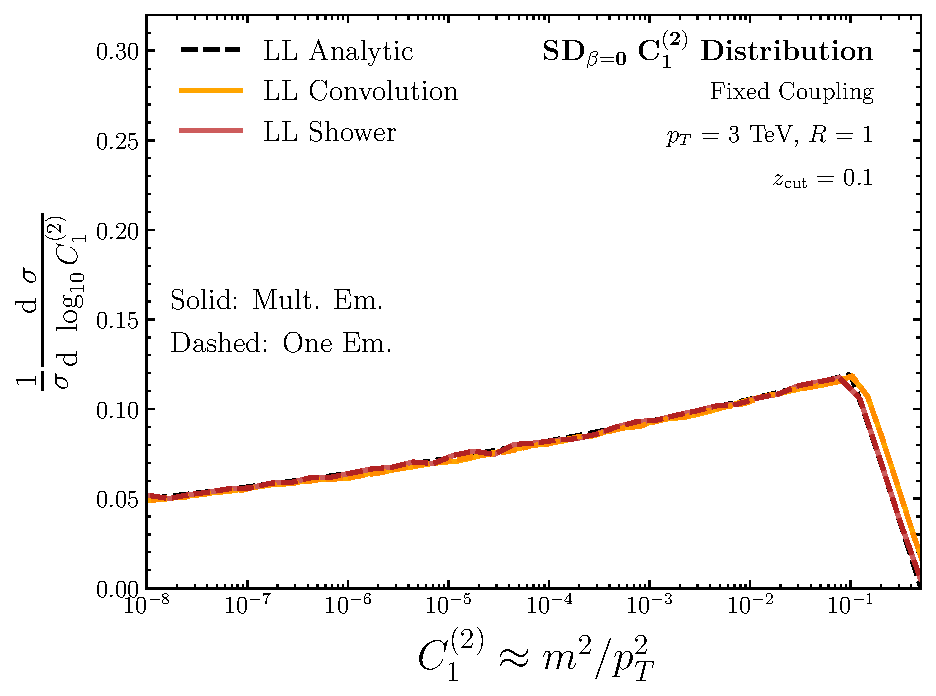
\includegraphics[width=.48\textwidth]{figures/piranha/resummed_plots/C12_SD0_LL}
\label{fig:LL_SD0}
}
%
% Soft Drop, MLL
\subfloat[]{
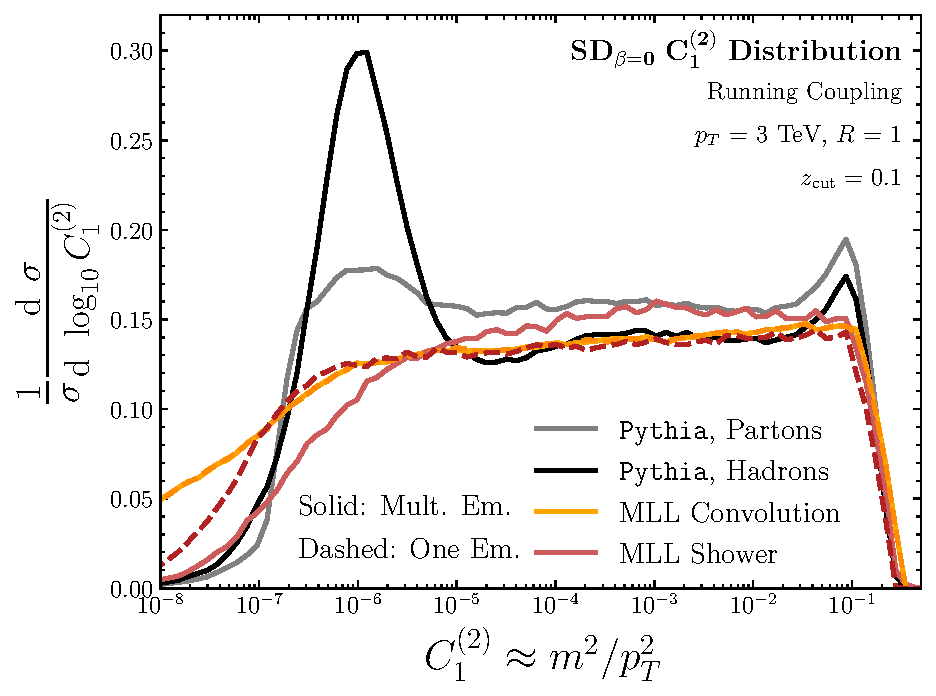
\includegraphics[width=.48\textwidth]{figures/piranha/resummed_plots/C12_SD0_MLL}
\label{fig:MLL_SD0}
}
\\
%
% \PRSF{1}, LL
\subfloat[]{
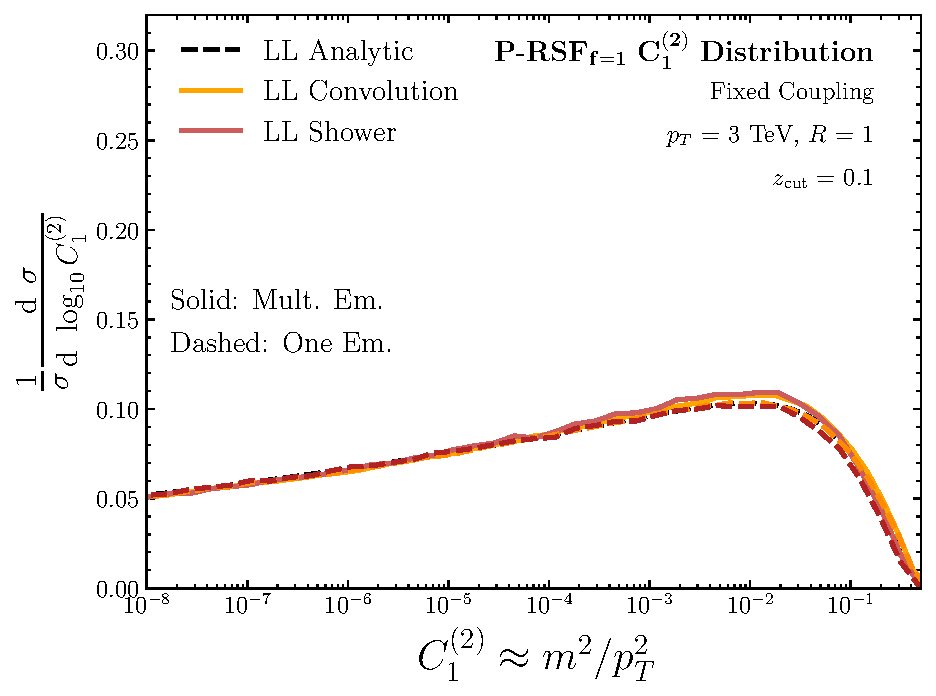
\includegraphics[width=.48\textwidth]{figures/piranha/resummed_plots/C12_PRSF1_LL}
\label{fig:LL_PRSF1}
}
%
% \PRSF{1}, MLL
\subfloat[]{
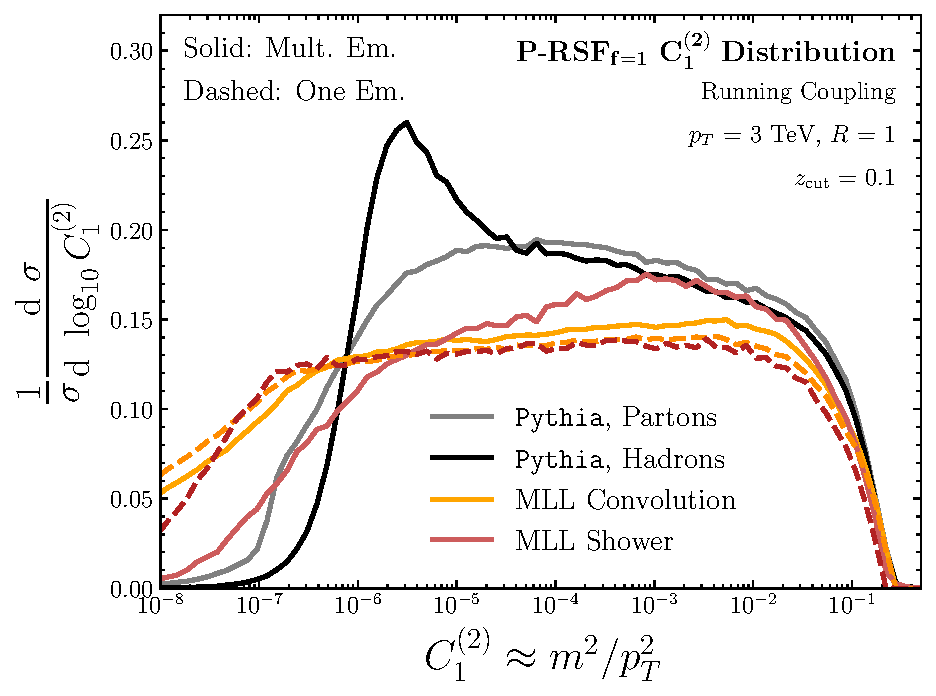
\includegraphics[width=.48\textwidth]{figures/piranha/resummed_plots/C12_PRSF1_MLL}
\label{fig:MLL_PRSF1}
}
\caption[Distributions of the observable \(C_1^{(2)}\approx m^2 / p_T^2\) for quark jets groomed with \SD{0} and \PRSF{1}.]{
Distributions of the observable \(C_1^{(2)}\approx m^2 / p_T^2\) of \Eq{ECFdefn_repeat} for quark jets groomed with \SD{0} (top row) and \PRSF{1} (bottom row), with and without multiple emissions, at (left column) LL accuracy and (right column) MLL accuracy.
%
For each plot, we display the results of the convolution method of \Eq{convolution} using numerical integration and \gls{pqcd} with \(10^6\) phase space samples as well as our own parton shower algorithm, discussed in \Prob{parton-shower} and its solution.
%
At LL, we compare these results to the analytic prediction of \Eq{ECF_LL};
%
at MLL, we compare them to parton-level and hadron-level results obtained with \texttt{Pythia 8.244} using the anti-\(k_t\) algorithm.
%
The figures demonstrate that \PRSF{1} is less sensitive to \gls{hadronization} corrections in the large observable regime, near \(C_1^{(2)} \approx 10^{-2}\), and that \PRSF{1} groomed substructure is more sensitive to the effects of multiple emissions than that of Soft Drop.
}
\label{fig:Calculations}
\end{figure}

As a result, performing resummed calculations of Soft Drop groomed substructure distributions that use only the critical emissions are more accurate than calculations for \PRSF{1} that only use the critical emission.
%
The relative accuracy of the LL, single-emission result for Soft Drop and \PRSF{1} is demonstrated in \Figs{LL_SD0}{LL_PRSF1}, which compares the fixed-order behavior of \(C_1^{(2)}\) distributions for jets groomed with Soft Drop or \PRSF{1}, respectively, using either the critical emission or all emissions in the jet.
%
Our parton shower procedure is inspired by \Reff{Larkoski:2013paa} and is exposed in more detail in Problem~\ref{prob:parton-shower}.
%
Including multiple emissions does not dramatically change the Soft Drop substructure distribution, but leads to non-negligible changes in \PRSF{1} substructure distributions.


%=====================================
% Modified Leading Logarithmic Calculation
%=====================================
We include effects from the running of the strong coupling constant and multiple emissions within the ungroomed jet to determine the behavior of the cumulative distribution of \(C_1^{(\varsigma)}\) at MLL accuracy.
%
While including these features in our calculation does not fully achieve next-to-leading-logarithmic (NLL) accuracy, the MLL calculation is an important piece of the full NLL result.
%
To consider the effects of several emissions on the distribution of the groomed ECFs, we convolve the probability distributions of several emissions that contribute to the total observable \(C_1^{(\varsigma)}\):

\begin{equation}
\begin{aligned}
    \rho^{\rm (MLL)}_\varsigma(C_{\rm tot})
    &=
    \int_{f\,\zcut}^{1/2} \dd \zcrit
    \int_0^R \dd \thetacrit
    ~
    \rho_{\rm crit}(\thetacrit)
    \rho_{\rm crit}(\zcrit | \zpre)
    \\
    &~~~
    \int \dd \zpre
    ~
    \rho_{\rm pre}(\zpre|\thetacrit)
    \int \dd c_{\rm sub}
    ~
    \rho_{\rm sub}(c_{\rm sub}|\zcrit,\thetacrit)
    \\
    &~~~~~~~~~~~~~~~
    \delta\left(
        C_{\rm tot}
        -
        C^{(\varsigma)}_{1,~\rm crit}
        (\thetacrit, \zcrit, \zpre)
        -
        c_{\rm sub}
    \right)
    \label{eq:convolution}
    .
\end{aligned}
\end{equation}

Each factor of \(\rho\) in \Eq{convolution} indicates a resummed probability distribution corresponding to a particular emission.
%
At the MLL level of accuracy, these resummed probability distributions are all calculated with a running coupling \(\alpha_s\).
%
We model non-perturbative effects by freezing the value of \(\alpha_s\) below the non-perturbative scale of \(\mu_{\rm freeze} = 1\) GeV, as in \Eq{frozen-coupling}.
%
Variations in our choice of non-perturbative scale lead only to small changes to our results.


The expressions that describe multiple emissions within the groomed jet are:
\begin{itemize}
\item
\(\rho_{\rm crit}(\thetacrit) \rho(\zcrit | \zpre)\) represents the probability distribution for the emission angle \(\thetacrit\) and energy fraction \(\zcrit\) of the \textit{critical} emission, or the first emission to survive the \PRSF{1/2} procedure.
%
This distribution is conditioned on the presence of earlier emissions that modify the grooming procedure.

\item
\(\rho_{\rm pre}(\zpre | \thetacrit)\) encodes the probability that emissions that are wider than the critical emission, which we call \textit{pre-critical} emissions, have an energy fraction \(\zpre\).
%
%Here, \textit{dominant} means that this is the pre-critical emission with the largest value of the energy fraction \(\zpre\).
%
Any non-zero value of \(\zpre\) mitigates the grooming of the critical emission.

\item
\(\rho_{\rm sub}(c_{\rm sub} | \zcrit, \thetacrit)\) is the probability distribution for emissions narrower than the critical emission to contribute a value \(c_{\rm sub}\) to the overall observable \(C^{(\varsigma)}_1\).
%
We call these emissions \textit{subsequent} emissions, and they are unmodified by the grooming procedure.

\item
Finally, \(C^{(\varsigma)}_{1,~\rm crit}(\thetacrit,\zcrit,\zpre)\) is the contribution of the critical emission to \(C^{(\varsigma)}_{1,~\rm tot}\), in the presence of pre-critical emissions with energy fraction \(\zpre\).
\end{itemize}

\remark{}{
    We examine the effects of \glspl{precrit-emission} and \glspl{sub-emission} on \gls{rsf}-groomed \gls{gecf} distributions, including multiple emissions effects, using the multiple emissions formula \Eq{resummed-multiple-emissions} exposited by Problem~\ref{prob:multiple-emissions}.
    %
    In particular, if we have the radiator for an additive observable \(\mathcal O\), it is simple to evaluate corrections due to the presence of multiple emissions with Laplace transform methods \cite{Banfi:2004yd} to find that, at MLL accuracy,
    %
    \begin{align}
        \Sigma^{\rm (MLL)}_{\mathcal O}(x)
        &=
       \frac{
       e^{-R_{\mathcal O}(x)
       -
       \gamma_E R'_{\mathcal O}(x)}
       }
       {\Gamma
       \left(1 + R'_{\mathcal O}(x)\right)
       }
       \label{eq:mll_general_dist}
       ,
    \end{align}
    %
    where \(\gamma_E\) is the Euler-Mascheroni constant, and the prime denotes a derivative with respect to \(\log(1/x)\), lead us to the MLL expressions for the effects of multiple pre-critical and subsequent emissions on jet ECFs.
    %
    For example, the cumulative distribution for the contribution of the subsequent emissions to the observable \(C_1^{(\varsigma)}\) takes the form
    %
    \begin{align}
        \Sigma^{\rm(MLL)}_{C^{(\varsigma)}_{\rm sub}}
        (C  |  \thetacrit, \zcrit)
        &=
       \frac{
       e^{-R_{\rm sub}(C)
       -
       \gamma_E R'_{\rm sub}(C)}
       }
       {\Gamma
       \left(1 + R'_{\rm sub}(C)\right)
       }
       \approx
       e^{-R_{\rm sub}(C)}
       =
       \Sigma^{\rm(LL)}_{C^{(\varsigma)}_{\rm sub}}
       (C  |  \thetacrit)
       \label{eq:subsequentDist}
       ,
    \end{align}
    %
    where \(R_{\rm sub}(C)\) is shorthand for \(R_{C^{(\varsigma)}_{\rm sub}}(C | \thetacrit)\), defined as
    %
    \begin{align}
        R_{C^{(\varsigma)}_{\rm sub}}
        (C | \thetacrit)
        &=
        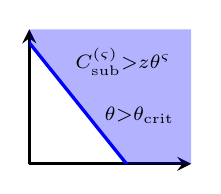
\begin{tikzpicture}[
        baseline={([yshift=-.8ex]current bounding box.center)},
        vertex/.style={anchor=base,
        circle,fill=black!25,minimum size=18pt,inner sep=2pt},
        scale=.3]
        \begin{axis}
        [xmin=0, xmax=5,
        ymin=0, ymax=5,
        axis line style = very thick,
        axis y line*=left,
        axis x line*=bottom,
        axis lines = middle,
        ticks=none]
            \addplot[name path=f,domain=0:5,
            style=very thick, blue]
            {4.5-1.5*x};
            \path[name path=axis]
            (axis cs:0,5) -- (axis cs:5,5);
            \addplot [
                thick,
                color=blue,
                fill=blue,
                fill opacity=0.3
            ]
            fill between[
                of=f and axis
            ];
            \node at (axis cs:  2.9,  3.8)
            {${\scriptstyle C_{\rm sub}^{(\varsigma)} > z\theta^\varsigma}$};
            \node at (axis cs:  3.4,  1.8)
            {${\scriptstyle \theta > \theta_{\rm crit}}$};
        \end{axis}
        \end{tikzpicture}
        =
        \int_{C/\thetacrit^{\varsigma}}^{1/2}
        \frac{\dd c}{c}
        \int_c^{1/2} \dd z\,
        \bar{p}_i(z)
        \frac{\alpha_s(\kappa)}{k \varsigma}
        .
    \end{align}
    Of course, the value of \zcrit{} will also have an impact on the subsequent emissions, but we may safely neglect these corrections, which contribute only by scaling \(C_{\rm sub}^{(\varsigma)}\) by factors of the form \(1 - \zcrit\).
    %
    The cumulative distribution for the energy fraction carried by pre-critical emissions is calculated similarly and takes the form
    %
    \begin{align}
        \Sigma^{\rm(MLL)}_{\zpre}
        (z | \thetacrit)
        &=
       \frac{
       e^{-R_{\rm pre}(z | \thetacrit)
       -
       \gamma_E R'_{\rm pre}(z | \thetacrit)}
       }
       {\Gamma
       \left(1 + R'_{\rm pre}(z | \thetacrit)\right)
       }
       \approx
       e^{-R_{\rm pre}(z | \thetacrit)}
       =
       \Sigma^{\rm(LL)}_{\zpre}
       (z  |  \thetacrit)
       \label{eq:preDist}
       ,
    \end{align}
    %
    where \(R_{\rm pre}(z | \thetacrit) = R_{\zpre}(z | \thetacrit)\) is given by
    %
    \begin{align}
        R_{\zpre}
        (z | \thetacrit)\
        &=
        \int_{\thetacrit}^{1}
        \frac{\dd\theta}{\theta}
        \int_{z}^{\zcut}\dd z'\,
        \bar{p}_i(z')
        \frac{\alpha_s(\kappa)}{\pi}
        .
    \end{align}
}

We evaluate the convolution of \Eq{convolution} -- including effects from the \gls{crit-emission}, \glspl{precrit-emission} and \glspl{sub-emission} -- through numerical integration, and compare the resulting distributions to the results from running coupling parton showers and \texttt{Pythia 8.244} in \Fig{Calculations}.
%
In particular, \Figs{MLL_SD0}{MLL_PRSF1} compare our numerical MLL results to hadron-level results for anti-\(k_t\) jets in \texttt{Pythia 8.244} and demonstrate that this trend of comparatively large multiple-emissions effects in \PRSF{1} continues at MLL.

First, let us note the difference between our MLL results obtained with Monte Carlo integration and via parton showers (as in Problem~\ref{prob:parton-shower}).
%
Our Monte Carlo results use a frozen coupling below a non-perturbative scale \(\mu_{\rm freeze} = 1\) GeV (see, for example, \Eq{frozen-coupling} of \App{soft-distortions}).
%
Our parton shower results both freeze the coupling at \(\mu_{\rm freeze} = 1\) GeV and stop the shower below a non-perturbative cutoff \(\mu_{\rm cutoff} = 1\) MeV, tuned by hand to match results from \texttt{Pythia 8.244}.
%
The shower cutoff effectively sets \(\alpha_s\) to zero below the scale set by \(\mu_{\rm cutoff}\).
%
Therefore, the plots in \Figs{MLL_SD0}{MLL_PRSF1} effectively show the results obtained with three different models of non-perturbative effects, with \texttt{Pythia 8.244} the most accurate.
%
Our MLL parton shower results in \Figs{MLL_SD0}{MLL_PRSF1} are still normalized, but the normalization is not immediately evident due to the presence of zero bins that are not shown in the logarithmically-scaled figures.
%
In passing from our rough parton shower model to the more accurate \gls{hadronization} model of \texttt{Pythia}, we expect that it is these zero bins that contribute to the additional hadron-level peak shown in the \texttt{Pythia} data.

We also point out that in \Fig{MLL_SD0}, the parton-level \texttt{Pythia 8.244} distribution for \(C_1^{(2)}\) also has an additional peak near the discontinuity in the parton-level LL result, in the regime of relatively large \(C_1^{(2)} \approx 10^{-1}\).
%
There is a comparable additional peak in the hadron-level \texttt{Pythia} distribution for \(C_1^{(2)}\) at this relatively large value for the observable.

We also note that, while our numerical results for \PRSF{1} in the MLL figures agree roughly with \texttt{Pythia 8.244} in the regime of large \(C_1^{(2)}\), the hadron-level \texttt{Pythia} distributions have an additional peak near \(C_1^{(2)} \approx 3\times 10^{-6}\) due to \gls{hadronization} corrections to the observable at that scale.
%
There is a similar additional peak in the hadron-level \texttt{Pythia} distribution for mMDT (\SD{0}) groomed \(C_1^{(2)}\).


% \begin{example}
%     \label{ex:conditionalprecrit}
%     Let's compute a conditional probability distribution relevant for the physics of Example \ref{ex:z_precrit}. In particular, let's compute the conditional probability distribution \(\rho(z_{\rm pre} | \theta_{\rm crit})\) to find a pre-critical emission with a maximum possible angle. We should first remember the solution to Example \ref{ex:z_precrit}, which gives us an overall probability distribution
%     \begin{equation}
%     \begin{aligned}
%         \rho(z_{\rm pre}, \theta_{\rm crit})
%         &=
%         \left(\frac{2 C_R \alpha_{\rm S}}{\pi}\right)^2
%         \frac{1}{\theta}
%         \log(\theta_{\rm crit})
%         [p(z_{\rm pre})]_+
%         \int_{z > z_{\rm pre}} z~\dd\log(z) [p(z)]_+
%         \\
%         &\ \ \ \ \ \ \ \ \ \ \
%         \times
%         \exp\left[
%         ~-~
%         \begin{tikzpicture}
%         [baseline={([yshift=-.8ex]current bounding box.center)},
%         vertex/.style={anchor=base,
%         circle,fill=black!25,minimum size=18pt,inner sep=2pt},
%         scale=.3]
%         \begin{axis}
%         [xmin=0, xmax=5,
%         ymin=0, ymax=5,
%         axis line style = very thick,
%         axis y line*=left,
%         axis x line*=bottom,
%         axis lines = middle,
%         ticks=none]
%             \addplot[name path=f,domain=0:2.3,
%             style=very thick,blue]
%             {2.5};
%             \addplot[very thick, samples=50, smooth,domain=0:6,blue, name path=three] coordinates {(2.3,-1)(2.3,2.5)};
%             \path[name path=axis]
%             (axis cs:0,0) -- (axis cs:2.3,0);

%             \addplot[name path=pre,domain=0:2.3,
%                     style=very thick,magenta]
%                     {2.6};
%             \addplot[name path=pre2,domain=0:2.3,
%                     style=very thick,magenta]
%                     {4.};
%             \addplot[very thick, samples=50, smooth,domain=0:6,magenta, name path=three] coordinates {(2.3,2.525)(2.3,4)};
%             \path[name path=axispre]
%             (axis cs:0,4) -- (axis cs:2.3,4);
%             \addplot [
%                 thick,
%                 color=blue,
%                 fill=blue,
%                 fill opacity=0.3
%             ]
%             fill between[
%                 of=f and axis
%             ];
%             \addplot [
%                 thick,
%                 color=magenta,
%                 fill=magenta,
%                 fill opacity=0.3
%             ]
%             fill between[
%                 of=pre and axispre
%             ];
%         \end{axis}
%         \end{tikzpicture}
%         ~~
%         \right]
%         .
%     \end{aligned}
%     \end{equation}


%     On the other hand, the probability distribution for \(\theta_{\rm crit}\) alone can be quickly read off from the solution to Example \ref{ex:theta_crit}:
%     \begin{equation}
%     \begin{aligned}
%         \rho(\theta_{\rm crit})
%         =
%         \frac{2 C_R \alpha_{\rm S}}{\pi}
%         ~
%         \frac{1}{\theta_{\rm crit}}
%         \int_{z > z_{\rm cut}} [p(z)]_+
%         ~~
%         \exp\left[
%         ~-~
%         \begin{tikzpicture}[
%         baseline={([yshift=-.8ex]current bounding box.center)},
%         vertex/.style={anchor=base,
%         circle,fill=black!25,minimum size=18pt,inner sep=2pt},
%         scale=.3]
%         \begin{axis}
%         [xmin=0, xmax=5,
%         ymin=0, ymax=5,
%         axis line style = very thick,
%         axis y line*=left,
%         axis x line*=bottom,
%         axis lines = middle,
%         ticks=none]
%         	\addplot[name path=f,domain=0:2.3,
%             style=very thick,blue]
%             {2.5};
%             \addplot[very thick, samples=50, smooth,domain=0:6,blue, name path=three] coordinates {(2.3,-1)(2.3,2.5)};
%             \path[name path=axis]
%             (axis cs:0,0) -- (axis cs:2.3,0);
%             \addplot [
%                 thick,
%                 color=blue,
%                 fill=blue,
%                 fill opacity=0.3
%             ]
%             fill between[
%                 of=f and axis
%             ];
%         \end{axis}
%         \end{tikzpicture}
%         ~~
%         \right]
%         .
%     \end{aligned}
%     \end{equation}

%     Finally, we can easily write the corresponding conditional probability
%     \begin{equation}
%     \begin{aligned}
%         \rho(z_{\rm pre}|\theta_{\rm crit})
%         &=
%         \frac{\rho(z_{\rm pre},\theta_{\rm crit})}{\rho(\theta_{\rm crit})}
%         \\
%         &=
%         \frac{2 C_R \alpha_{\rm S}}{\pi}
%         ~
%         \log(\theta_{\rm crit})
%         ~
%         [p(z_{\rm pre})]_+
%         ~
%         \frac{\int_{z > z_{\rm pre}} z~\dd\log(z) p(z)}
%         {\int_{z > z_{\rm cut}} z~\dd\log(z) p(z)}
%         ~~
%         \exp\left[
%         ~-~
%         \begin{tikzpicture}
%         [baseline={([yshift=-.8ex]current bounding box.center)},
%         vertex/.style={anchor=base,
%         circle,fill=black!25,minimum size=18pt,inner sep=2pt},
%         scale=.3]
%         \begin{axis}
%         [xmin=0, xmax=5,
%         ymin=0, ymax=5,
%         axis line style = very thick,
%         axis y line*=left,
%         axis x line*=bottom,
%         axis lines = middle,
%         ticks=none]
%             \addplot[name path=pre,domain=0:2.3,
%                     style=very thick,magenta]
%                     {2.6};
%             \addplot[name path=pre2,domain=0:2.3,
%                     style=very thick,magenta]
%                     {4.};
%             \addplot[very thick, samples=50, smooth,domain=0:6,magenta, name path=three] coordinates {(2.3,2.525)(2.3,4)};
%             \path[name path=axispre]
%             (axis cs:0,4) -- (axis cs:2.3,4);
%             \addplot [
%                 thick,
%                 color=magenta,
%                 fill=magenta,
%                 fill opacity=0.3
%             ]
%             fill between[
%                 of=pre and axispre
%             ];
%         \end{axis}
%         \end{tikzpicture}
%         ~~
%         \right]
%         \\
%         &\approx
%         \frac{2 C_R \alpha_{\rm S}}{\pi}
%         ~
%         \log(\theta_{\rm crit})
%         ~
%         \left[\frac{1}{z_{\rm pre}}\right]_+
%         \frac{\log(z_{\rm cut} / z_{\rm pre})}{\log(z_{\rm cut})}
%         ~
%         z_{\rm pre}^{~~\frac{2 C_R \alpha_{\rm S}}{\pi}\log(\theta_{\rm crit})}.
%     \end{aligned}
%     \end{equation}
% \end{example}

We need only use the singular pieces of the splitting functions to achieve LL accuracy, but, by definition, we must include the non-singular pieces of the splitting functions to achieve MLL accuracy.
%
While the MLL analysis modifies the LL analysis by including additional, higher-order behavior, it is not quite sufficient to produce results at next-to-leading logarithmic (NLL) accuracy;
%
a full NLL result requires a more intricate treatment including the effects of logarithms due to the constraint that radiation within the jet must lie within the jet radius.
%
These logarithms emerge because jet observables depend on only subsets of the full phase (global) space of the outgoing radiation, and are known as non-global logarithms \cite{Dasgupta:2001sh,Dasgupta:2002dc,Dasgupta:2002bw,Banfi:2002hw,Appleby:2002ke,Weigert:2003mm,Rubin:2010fc,Banfi:2010pa,Kelley:2011tj,Hornig:2011iu,Kelley:2011aa,Hatta:2013iba,Schwartz:2014wha,Khelifa-Kerfa:2015mma,Larkoski:2015zka,Larkoski:2016zzc,Banfi:2021owj}.
%
Regardless, the MLL results presented in the paper provide a sense of the physics contained within NLL results.



%==============================================
\section{Discontinuities in Grooming}
%==============================================
\label{sec:discontinuity}

In this section, we examine the formal structure of discontinuities in grooming in greater detail, and explore the improved continuity of \PIRANHA{} conceptually through several toy examples.
%
We compare the leading order (LO) soft continuity properties of Soft Drop and Recursive Subtraction both conceptually (\Sec{sd_discont}) and through a perturbative calculation (\Sec{sd_discont_lo}).
%
In \Secs{rsf_discont}{ang_discont}, we explore potential challenges to continuity that can arise in more intricate scenarios.
%
In particular, a key result of this section is that it is \textit{impossible} to design a fully continuous, tree-based \gls{declustering} algorithm.
%
Specifically, we discuss suppressed soft discontinuities that emerge in Unbalanced Recursive Subtraction (\Sec{rsf_discont}) and angular discontinuities induced by angular-ordered jet clustering that emerge beyond \glslink{accuracy}{NLO} in tree-based grooming algorithms (\Sec{ang_discont}).
%
We do not delve into the mathematical intricacies or perturbation theory of these examples, and they may be skipped on an initial reading.
%
The qualitative continuity properties explored in this section are also summarized at the beginning of the chapter, and contrasted against the discontinuities of traditional groomers, in \Tab{groomerlist}.
%
We explore the improved continuity of \PIRANHA{} groomers in a more practical context in \Sec{grooming-pheno}, where we study the responses of \PIRANHA{} grooming to several sources of \glspl{soft-distortion} and \gls{additive-contamination}.


The modified Mass Drop Tagger (mMDT, or \SD{0}) \cite{Dasgupta:2013ihk,Larkoski:2014wba}, for example, requires that certain sub-jets within a jet carry a sufficient energy fraction, \(z > z_{\rm cut}\), to survive the grooming procedure.
%
If a sub-jet has an energy fraction near \(\zcut\), low-energy pollution may push its energy to the other side of the cutoff, leading to soft discontinuous behavior and associated theoretical and experimental complications.
%
\Fig{grooming-cartoon} demonstrates this soft discontinuous behavior, and the corresponding soft continuity of \PRSF{1/2}, by comparing their action on two sets of similar events:
%
two toy jet events \(\mathcal{E}^\pm\) consisting of two particles each, and a QCD jet produced in \texttt{Pythia 8.244} along with the same QCD event with a small amount of gaussian noise applied to the \(p_T\), rapidity, and azimuthal angle of each particle.
%
We revisit the events \(\mathcal{E}^\pm\) as tools to characterize soft discontinuity more precisely in \Sec{sd_discont}.
%
The mMDT grooming procedure maps \(\mathcal{E}^+\) and \(\mathcal{E}^-\) to very distinct events, and similarly maps the noiseless and noisy QCD jets to very distinct groomed jets.
%
We chose an unusually high value of \(\zcut = 0.25\) when grooming the QCD events to make the discontinuity of mMDT more apparent.
%
\footnotetext{
Soft Drop with \(\beta_{\rm SD} \leq 0\) is not collinear safe in grooming mode, used in this thesis, where jets consisting of a single particle are retained as groomed jets.
%
Grooming mode is a natural choice in the context of \gls{pu-mitigation} (see \Sec{sd_discont}).
%
Note that Soft Drop with \(\beta_{\rm SD} \leq 0\) is collinear safe in tagging mode, where jets consisting of a single particle are groomed away completely.
}

%=====================================
% Simple Demonstration of Continuity:
%=====================================
\subsection{An Invitation to Soft Discontinuities: Soft Drop Versus P-RS}
\label{sec:sd_discont}

%-----------------------------------
% Cartoon of comparison:
%-----------------------------------
\begin{figure}[]
\centering
\scalebox{0.95}{
    \begin{tikzpicture}[baseline=-3.5ex]
% Event Labels
  \node at (-1.7,  .6)()
        {\huge \(\mathcal{E}^+\)};
  \node at (-1.7,  -1.25)()
        {\huge\(\mathcal{E}^-\)};

% Header wrapper
\draw [fill=black, opacity=0.05]
       (-0.7,2.4) -- (13.6,2.4) -- (13.6,1.65) -- (-0.7,1.65) -- cycle;

%%%%%%%%%%%%%%
% Ungroomed
%%%%%%%%%%%%%%
  \node at (1.5,  2)() {\textbf{Ungroomed}};

% E+
  % points
  \coordinate (A)  at (1.4, 1.4);
  \coordinate (O)  at (0, 0);
  \coordinate (B)  at (3, 0);
  % legs
  \draw[-Stealth,line width=.55mm] (O) -> (A);
  \draw[-Stealth,line width=.7mm] (O) -> (B);

% E-
  % points
  \coordinate (A)  at (.8, -1.2);
  \coordinate (O)  at (0, -2);
  \coordinate (B)  at (3, -2);
  % legs
  \draw[-Stealth,line width=.55mm] (O) -> (A);
  \draw[-Stealth,line width=.7mm] (O) -> (B);

% lines

% zcut lines
\coordinate (I)  at (0.7, 1.0);
\coordinate (F)  at (3.15, 1.0);
\draw[dash pattern=on 2pt off 3pt, line width=.4mm, color=aurometalsaurus] (I) -> (F);
\node at (3.5,  1.0)()
        {\(\zcut\)};

\coordinate (I)  at (0.7, -1.0);
\coordinate (F)  at (3.15, -1.0);
\draw[dash pattern=on 2pt off 3pt, line width=.4mm, color=aurometalsaurus] (I) -> (F);
\node at (3.5,  -1.0)()
        {\(\zcut\)};

% Descriptors
\node [rotate=45] at (0.0,  0.5)()
        {\(z^+ > \zcut\)};
\node [rotate=45] at (0.0,  -1.5)()
        {\(z^- < \zcut\)};


%%%%%%%%%%%%%%
% Soft Drop Grooming
%%%%%%%%%%%%%%
\node at (6.5,  2)() {\textcolor{dodgerblue!75!black}{\textbf{Soft Drop}, \(\beta_{\rm SD} = 0\)}};

% E+
  % points
  \coordinate (A)  at (6.4, 1.4);
  \coordinate (O)  at (5.0, 0);
  \coordinate (B)  at (8.0, 0);
  % legs
  \draw[-Stealth,line width=.55mm, color=royalblue] (O) -> (A);
  \draw[-Stealth,line width=.7mm, color=royalblue] (O) -> (B);

% E-
  % points
  \coordinate (Ap)  at (5.8, -1.2);
  \coordinate (O)  at (5.0, -2);
  \coordinate (B)  at (8.0, -2);
  % legs
  \draw[-Stealth, line width=.55mm, color=black!25!white] (O) -> (Ap);
  \draw[-Stealth,line width=.7mm, color=royalblue] (O) -> (B);

% lines
% zcut lines
\coordinate (I)  at (5.7, 1.0);
\coordinate (F)  at (8.15, 1.0);
\draw[dash pattern=on 2pt off 3pt, line width=.4mm, color=aurometalsaurus] (I) -> (F);

\coordinate (I)  at (5.7, -1.0);
\coordinate (F)  at (8.15, -1.0);
\draw[dash pattern=on 2pt off 3pt, line width=.4mm, color=aurometalsaurus] (I) -> (F);

%%%%%%%%%%%%%%
% PIRANHA Grooming \PRSF{1/2}
%%%%%%%%%%%%%%
  \node at (10.9,  2)() {\textcolor{ochre!75!black}{\textbf{P-RSF} (arb.\,\(f_{\rm soft}\))}};

% E+
  % points
  \coordinate (A)  at (10.4, 0.9);
  \coordinate (Ap)  at (10.9, 1.4);
  \coordinate (O)  at (9.5, 0);
  \coordinate (B)  at (11.7, 0);
  \coordinate (Bp)  at (12.5, 0);
  % legs
  \draw[-Stealth,line width=.55mm, color=black!25!white] (O) -> (Ap);
  \draw[-Stealth,line width=.55mm, color=darkgoldenrod] (O) -> (A);
  \draw[-Stealth,line width=.7mm, color=black!25!white] (O) -> (Bp);
  \draw[-Stealth,line width=.7mm, color=darkgoldenrod] (O) -> (B);

% E-
  % points
  \coordinate (A)  at (9.9, -1.6);
  \coordinate (Ap)  at (10.3, -1.2);
  \coordinate (O)  at (9.5, -2);
  \coordinate (B)  at (11.7, -2);
  \coordinate (Bp)  at (12.5, -2);
  % legs
  \draw[-Stealth,line width=.55mm, color=black!25!white] (O) -> (Ap);
  \draw[-Stealth,line width=.55mm, color=darkgoldenrod] (O) -> (A);
  \draw[-Stealth,line width=.7mm, color=black!25!white] (O) -> (Bp);
  \draw[-Stealth,line width=.7mm, color=darkgoldenrod] (O) -> (B);

% lines
% zcut lines
\coordinate (I)  at (10.2, 1.0);
\coordinate (F)  at (12.65, 1.0);
\draw[dash pattern=on 2pt off 3pt, line width=.4mm, color=aurometalsaurus] (I) -> (F);

\coordinate (I)  at (10.2, -1.0);
\coordinate (F)  at (12.65, -1.0);
\draw[dash pattern=on 2pt off 3pt, line width=.4mm, color=aurometalsaurus] (I) -> (F);

%%%%%%%%%%%%%%
% QCD
%%%%%%%%%%%%%%
% Double line
\coordinate (I)  at (-2.5, -2.8);
\coordinate (F)  at (13.3, -2.8);
\draw[line width=.3mm] (I) -> (F);

\coordinate (I)  at (-2.5, -2.9);
\coordinate (F)  at (13.3, -2.9);
\draw[line width=.3mm] (I) -> (F);

% Labels
  \node at (-1.7,  -4.6)()
        {\textbf{\LARGE QCD}};
  \node at (-2.55, -5.8)(){\Large (};
  \node at (-1.7,  -5.6)()
        {\texttt{Pythia}};
  \node at (-1.7,  -6.0)()
        {\texttt{8.244}};
 \node at (-0.85, -5.8)(){\Large )};
  \node at (-1.7,  -8.4)()
         {\textbf{\LARGE QCD}};
 \node at (-1.7,  -9.0)()
         {\textbf{\Large +}};
 \node at (-1.7,  -9.6)()
        {\textbf{\LARGE Noise}};

% Event visualization
% Ungroomed
  \node at (1.8,  -5.0)() {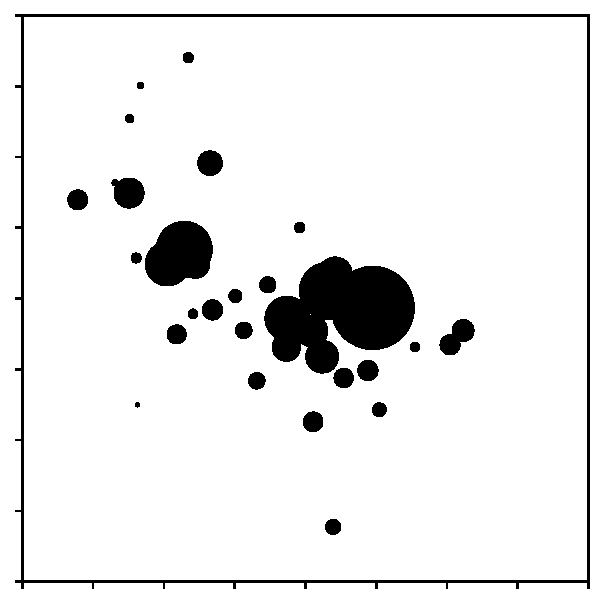
\includegraphics[width=.25\textwidth]{figures/piranha/event_visualizations/vis_raw_1}};
  \node at (1.8,  -9.0)() {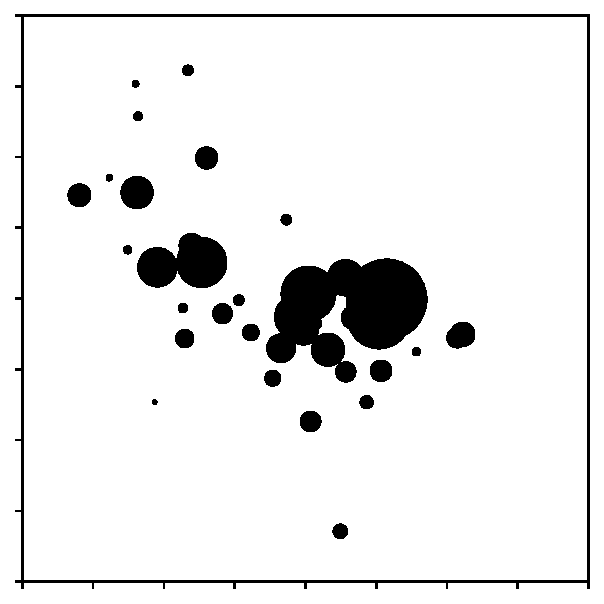
\includegraphics[width=.25\textwidth]{figures/piranha/event_visualizations/vis_raw_2}};
% mMDT
  \node at (6.5,  -5.0)() {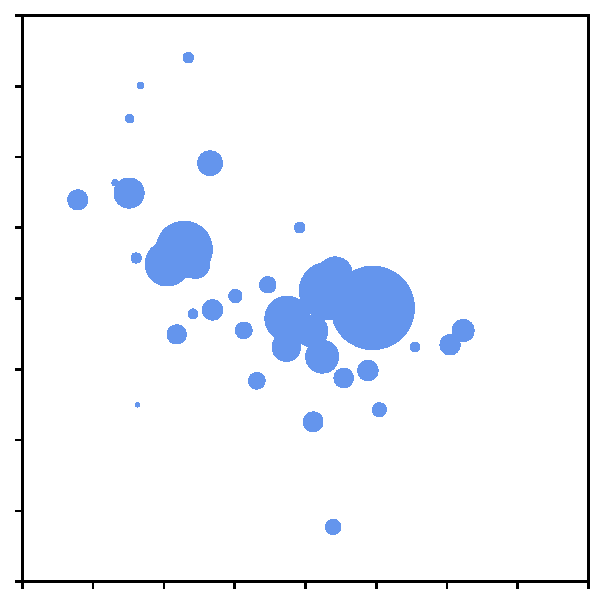
\includegraphics[width=.25\textwidth]{figures/piranha/event_visualizations/vis_mmdt_1}};
  \node at (6.5,  -9.0)() {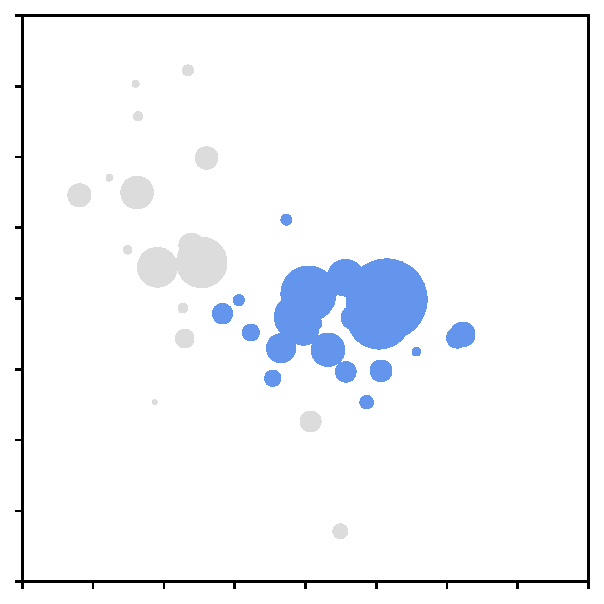
\includegraphics[width=.25\textwidth]{figures/piranha/event_visualizations/vis_mmdt_2}};
% P-RSF_1/2
  \node at (11.3,  -5.0)() {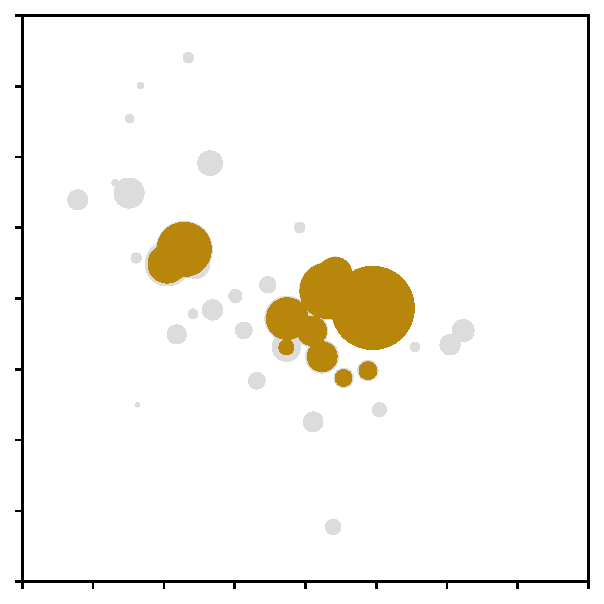
\includegraphics[width=.25\textwidth]{figures/piranha/event_visualizations/vis_rsf_half_1}};
  \node at (11.3,  -9.0)() {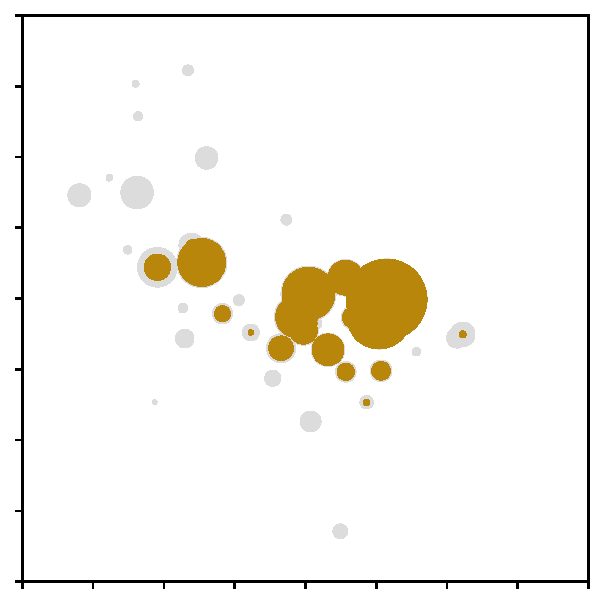
\includegraphics[width=.25\textwidth]{figures/piranha/event_visualizations/vis_rsf_half_2}};

% Axis info
 \node at (-0.4,  -5.0)() {\Large \(\phi\)};
 \node at (-0.4,  -9.0)() {\Large \(\phi\)};
 \node at (1.8,  -11.2)() {\Large \(y\)};
 \node at (6.5,  -11.2)() {\Large \(y\)};
 \node at (11.3,  -11.2)() {\Large \(y\)};

 % phi labels
 \node at (-0.25,  -10.77)() {\footnotesize -1};
 \node at (-0.25,  -7.3)() {\footnotesize 1};
 \node at (-0.25,  -6.77)() {\footnotesize -1};
 \node at (-0.25,  -3.3)() {\footnotesize 1};
 % y labels
 \node at (-0.05,  -11.1)() {\footnotesize -1};
 \node at (3.65,  -11.1)() {\footnotesize 1};
 \node at (4.65,  -11.1)() {\footnotesize -1};
 \node at (8.35,  -11.1)() {\footnotesize 1};
 \node at (9.45,  -11.1)() {\footnotesize -1};
 \node at (13.15,  -11.1)() {\footnotesize 1};

 %\node at (1.8,  -5.0)() {-1.0};
\end{tikzpicture}

}
\caption[A cartoon comparing the discontinuous action of hard-cutoff grooming to the continuous action of \PIRANHA{}.]{
A cartoon comparing the discontinuous action of hard-cutoff grooming to the continuous action of \PIRANHA{} on the nearly identical two-particle events with energy \(Q\), \(\mathcal{E}^+\) and \(\mathcal{E}^-\).
%
We use Soft Drop (with \(\beta_{\rm SD} = 0\)) and P-RSF (with arbitrary \(f_{\rm soft}\)) with a grooming parameter \zcut{} as representative examples of the hard-cutoff and \PIRANHA{} paradigms, respectively.
%========
% Ungroomed
%========
The events \(\mathcal E^\pm\) differ only by the energy fraction of the softer particle,
%
\(
z^\pm = \zcut \pm \delta/2
\),
%
and are separated by an infinitesimal EMD,
%
EMD\(
(\mathcal{E}^+, \mathcal{E}^-)
\sim \delta \ll \zcut
\).
%========
% SD
%========
Despite their similarity, Soft Drop maps the events to distinct groomed results separated by a large EMD:
%
%it removes no energy from \(\mathcal E^+\) (\(\Delta E^+_{\rm SD} = 0\)) and completely removes the softer particle from \(\mathcal E^-\) (\(\Delta E^-_{\rm SD} \sim Q z^-\)).
%
%and the Soft Drop groomed results are separated by a large EMD of
%
EMD\(
(\mathcal{E}_{\rm SD}^+, \mathcal{E}_{\rm SD}^-)
\sim \zcut \gg \delta
\).
%========
% P-RSF
%========
P-RSF instead
% subtracts a similar energy from both events (\(\Delta E^\pm_{\rm P\mhyphen RSF} \sim Q \zcut\)) and
maps the events continuously to infinitesimally similar groomed events:
%
EMD\(
(\mathcal{E}_{\rm P\mhyphen RSF}^+,
\mathcal{E}_{\rm P\mhyphen RSF}^-)
\sim \delta
\).
%
\(\Delta E^\pm_G\) indicates the amount of energy removed from the event \(\mathcal E^\pm\) by the groomer \(G\).
}
\label{fig:grooming-cartoon}
\end{figure}


%-----------------------------------
% Text comparison:
%-----------------------------------
Traditional groomers are discontinuous in the regions of parameter space near a hard cutoff.
%
For example, Soft Drop is discontinuous in the region of parameter space where
\(
    z_{\rm soft} = \zcut \theta^{\beta_{\rm SD}} / R_0^{\beta_{\rm SD}}
\)
due to the Soft Drop criterion of \Eq{softdropcriterion}.
%
In this subsection, we discuss the discontinuity of hard-cutoff grooming and the relative continuity of \PIRANHA{}.

The following discussion centers around the illustrative example shown in \Fig{grooming-cartoon}, which shows the simplest instance of discontinuous behavior near a hard cutoff as well as the resolution offered by \PIRANHA{}.
%
In this example, we consider two nearly identical events, \(\mathcal{E}^+\) and \(\mathcal{E}^-\), that each contain two particles.
%
The softer constituent of \(\mathcal E^+\) has an energy fraction \(z^+ =  \zcut + \delta\) slightly above the grooming parameter \zcut, while the softer constituent of \(\mathcal E^-\) has an energy fraction \(z^- =\zcut - \delta\) slightly below \zcut.
%
The energy flows of the two events are nearly indistinguishable, in the sense that \(
{\rm EMD}(\mathcal{E}^+, \mathcal{E}^-)\sim\delta
\),
and we choose \(\delta\) for consistency with Definition~\ref{def:eventcontinuity}.
%
We use Soft Drop with \(\beta_{\rm SD} = 0\), or mMDT, as a representative example of hard-cutoff grooming, and P-RSF with arbitrary \(f_{\rm soft}\) as a representative example of the \PIRANHA{} paradigm;
%
for each, we use the parameter \(\zcut\).

Soft Drop treats \(\mathcal E^+\) and \(\mathcal E^-\) very differently:
%
it does not modify \(\mathcal E^+\), but completely removes the softer particle of \(\mathcal E^-\).
%
The energy flow of \(\mathcal E^+\) is unchanged, while that of \(\mathcal E^-\) is changed dramatically, and the EMD between the groomed jets is relatively large:
EMD\(
(\mathcal{E}^+_{\rm SD},
\mathcal{E}^-_{\rm SD})
\sim \zcut
\gg \delta\).
%
Direct application of Definition~\ref{def:eventcontinuity} to our example shows that Soft Drop is discontinuous.\footnote{
We note that Soft Drop with \(\beta \neq 0\) is also soft discontinuous.
%
Indeed, the above arguments still hold for the case \(\beta \neq 0\), verbatim, when the angle between the particles of \(\mathcal E^\pm\) is fixed to \(\theta = R_0\).
%
As expressed in \Eq{softdropcriterion}, the Soft Drop criterion at this fixed angle is still \(z_{\rm soft} > \zcut\).
%
However, since Soft Drop with \(\beta \neq 0\) drops the softer particle if it does not satisfy \(z / \theta^{\beta} > \zcut/ R_0^\beta\), we may also say that Soft Drop with \(\beta \neq 0\) is ``\(z / \theta^{\beta}\)-discontinuous'', where \(z\)-discontinuity indicates the soft discontinuity for the case of \(\beta = 0\) that we discuss above.
}
%
Since the events \(\mathcal E^+\) and \(\mathcal E^-\) differ by small changes to the energy of jet constituents, we see that Soft Drop is soft discontinuous in the region of parameter space near the cutoff \zcut.

The procedure of P-RSF is quite different.
%
When grooming both events, \PRSF{1/2} grooms the energy of both emissions by the same amount, leading to no large discrepancy in the two groomed results.
%
Indeed, after the \PRSF{1/2} grooming procedure, these two events are still separated by an infinitesimal EMD:
EMD\((\mathcal{E}^+_{\rm RSF},
\mathcal{E}^-_{\rm RSF})\sim\delta\).
%
This simple example demonstrates how hard-cutoff grooming methods may discontinuously map two nearly identical events into vastly different groomed results, and showcases the soft continuous resolution of the \PRSF{1/2} grooming procedure and other \PIRANHA{} groomers.


%=====================================
% Discontinuity in SD in LO calculation
%=====================================

\subsection{Soft Discontinuities in Perturbation Theory}
\label{sec:sd_discont_lo}

Next, we examine the manifestations of the soft discontinuous behavior of hard-cutoff grooming more quantitatively by comparing the \gls{gecf} distributions of jets groomed with \gls{soft-drop} and \gls{rsf} at NLO.
%
The resummed analysis of \Sec{pira-resummed} does not change the qualitative conclusions of our discussion below.
%
However, it highlights subtleties in systematically improving our resummed substructure calculations due to the global, subtractive nature of \PIRANHA{} grooming.
%
Therefore, while our resummation does not change the qualitative conclusions of the following discussion, it indicates that the computation of resummed \PIRANHA{} observables at higher accuracy may require new calculational tools.


The probability distribution of \(C_1^{(\varsigma)}\) for Soft Drop was studied in \Reff{Larkoski:2014wba} (see Exercise~\ref{ex:soft-drop-gecf}), which found, for \(\beta_{\rm SD} > 0\), the \glslink{accuracy}{NLO} result
\begin{align}
    \label{eq:sd_lo}
    \rho_{i,\,\,\text{SD}}(C_1^{(\varsigma)})
    \approx
    \frac{2\alpha_s C_{R_i}}{\pi \varsigma} \frac{1}{C_1^{(\varsigma)}}
    \times
    \begin{cases}
        -\log C_1^{(\varsigma)} + B_i,
        &
        C_1^{(\varsigma)} > \zcut;
        \\
        -
        \frac{\beta_{\rm SD}}{\varsigma+\beta_{\rm SD}} \log C_1^{(\varsigma)}
        -
        \frac{\varsigma}{\varsigma+\beta_{\rm SD}}\log \zcut
        +
        B_i,
        &
        C_1^{(\varsigma)} < \zcut,
    \end{cases}
\end{align}
away from \(C_1^{(\varsigma)} = 0\), up to \(\mathcal{O}(\alpha_s^2)\) and terms that are power suppressed in \(C_1^{(\varsigma)}\), \zcut, or both.
%
\(B_i\) is a factor due to hard-collinear pieces of the splitting function that are not singular as \(z\) approaches 0:
%
$B_q = -3/4$ for quarks and $B_g = -11/12+N_f/(6 C_A)$ for gluons, where $N_f$ is the number of active quark flavors.
%
The case \(\beta_{\rm SD} < 0\) leads to an identical result up to another constraint on \(C_1^{(\varsigma)}\), which simply multiplies the expression above by \(\Theta(C_1^{(\varsigma)} > \zcut^{\varsigma/ |\beta_{\rm SD}|})\).

The piece-wise behavior of \Eq{sd_lo} and the associated kink in the Soft Drop \(C_1^{(\varsigma)}\) distribution are due to the discontinuous behavior of Soft Drop.
%
As noted by \Reff{Larkoski:2014wba}, when \(\beta_{\rm SD} \geq 0\) any two-parton configurations with \(C_1^{(\varsigma)} = z \, (\theta/R_0)^\varsigma \, > \, \zcut\) must have \(z \, (\theta/R_0)^{\beta_{\rm SD}} \, > \, \zcut\), and are therefore not affected by Soft Drop.
%
On the other hand, configurations with \(C_1^{(\varsigma)} < \zcut\) may be Soft Dropped, leading to the piece-wise change in groomed substructure in this region of phase space.

In Exercise~\ref{ex:rsf-gecf}, however, we found the \glslink{accuracy}{NLO} result
\begin{equation}
    \rho_{i,\,\,\text{P-RSF}}(C_1^{(\varsigma)}; f)
    \approx
    \frac{2\alpha_s C_{R_i}}{\varsigma~\pi}
    \frac{1}{C_1^{(\varsigma)}}
    \left(
        -\log\left(C_1^{(\varsigma)} + f\,\zcut\right)
        + B_i
    \right),
    \label{eq:prsf_NLO}
\end{equation}
away from \(C_1^{(\varsigma)} = 0\), using the same factors of \(B_i\) as for Soft Drop, and up to terms that are power-suppressed in \(C_1^{(\varsigma)}\), \(\zcut\), or both.%
\footnote{
    Up to virtual corrections, discussed in Remark~\ref{rem:recursive-subtraction-virtual}, and additional power-suppressed terms.
}

Notably, the P-RSF distribution for \(C_1^{(\varsigma)}\) is smooth and does not need to be defined in a piece-wise fashion.
%
Even at \glslink{accuracy}{NLO}, the subtractive nature of P-RSF leads to a smooth interpolation between double-logarithmic behavior at large \(C_1^{(\varsigma)}\) and single-logarithmic behavior at small \(C_1^{(\varsigma)}\).\footnote{The terms ``double logarithmic'' and ``single logarithmic'' here refer to the behavior of the \glslink{accuracy}{NLO} cumulative distribution function.
%
In particular, we note that when \(C_1^{(\varsigma)} \gg f\,\zcut\), the pseudo-probability distribution \(\rho \propto \log\left(C\right)/C\) demonstrates double-logarithmic behavior.
%
On the other hand, when \(0 < C_1^{(\varsigma)} \ll f\,\zcut\), the distribution \(\rho \propto \log\left(f\,\zcut\right)/C\) demonstrates single-logarithmic behavior.
}
%
Much as the kink in the Soft Drop distribution can be attributed to the sudden activation of the grooming procedure in certain regions of phase space, the smoothness of the P-RSF distribution reflects in part that the grooming procedure is always active.\footnote{
We say that the smoothness of P-RSF only reflects the global activity of the grooming \textit{in part} because we expect that \PIRANHA{} groomers that turn on gradually will also have smooth substructure distributions.}
%
While the piece-wise behavior of Soft Drop observable distributions is smoothed out by all-orders effects \cite{Benkendorfer:2021unv}, the smoothness of P-RSF observable distributions at \glslink{accuracy}{NLO} is a manifestation of the subtractive behavior of P-RSF that ensures its continuity on two-parton jets.

We also note that the substructure distributions of other \PIRANHA{} grooming procedures can be calculated at \glslink{accuracy}{NLO} with a similar method by upgrading \(f_{\rm soft}\) to a function of \(z\) and \(\theta\).
%
Further, we expect that such an \(f(z, \theta)\) may be well approximated by \(f(0,0)\), with sub-leading corrections proportional to \(\mathcal{O}(z, \theta, \zcut)\).

\remark{}{
    In our discussion above, we emphasized that the kinks in Soft Drop groomed substructure distributions are manifestations of the discontinuity of Soft Drop itself.
    %
    Generalizations of these arguments, however, must be verified carefully.
    %
    In particular, there is not generically a one-to-one correspondence between kinks in distributions and discontinuities in the associated observable.
    %
    As a toy one-dimensional example, consider a random variable \(X\) that is uniformly distributed in \((-1/2,\,1/2)\).
    %
    The discontinuous, ``zig-zagging'' function \(f(X) = X \pm 1/2\), choosing the upper sign for \(X < 0\) and the lower sign for \(X > 0\), is uniformly distributed.
    %
    Therefore, discontinuous functions on our toy ``phase space'' -- the domain of \(X\) -- do not necessarily have kinks in their distributions.
    %
    Conversely, there is a kink in the distribution of \(f(X) = \mp (1 - \sqrt{1 \pm 2X})/2\), where we take the upper sign when \(X < 0\) and the lower sign for \(X \geq 0\), even though \(f(x)\) is a continuous function of \(x\) and has a continuous first derivative.
}

%=====================================
% Discontinuity in P-RSF with \(f_{\rm soft}\neq1/2\)
%=====================================

\subsection{Suppressed Soft Discontinuities in Unbalanced P-RS}
\label{sec:rsf_discont}

Unbalanced P-RSF algorithms are also discontinuous in the suppressed region of parameter space where \(z = 1/2\).\footnote{
The probability density of seeing a softer sub-jet with energy fraction \(z\) scales as \(1/z\) at leading logarithmic accuracy in \gls{pqcd}.
%
Therefore, the region with \(z \sim 1/2\) at the boundary of the jet phase space is far less populated than the regions of phase space near a hard-cutoff with \(z \sim \zcut < 1/2\).
}
%
The discontinuous behavior emerges because Unbalanced P-RSF algorithms treat harder and softer sub-jets differently;
%
since an infinitesimally soft perturbation can lead to either sub-jet having more energy when \(z = 1/2\), an infinitesimal change in an ungroomed energy flow can lead to macroscopic differences in groomed results.
%
Concretely, we say that Unbalanced P-RSF is soft discontinuous in the suppressed, measure zero region of parameter space where \(z = 1/2\), and that Balanced P-RSF is the only soft continuous P-RSF algorithm.

In the following discussion, we explore the soft discontinuity of Unbalanced P-RS in the context of a jet containing only two partons.
%
We find that the discontinuity at \(z = 1/2\) can lead to macroscopic changes to the groomed jet axis.
%
However, only the orientation of the jet is affected by the soft discontinuity in our two-parton example, and the soft discontinuity of Unbalanced P-RS is not reflected at \glslink{accuracy}{NLO} by traditional jet substructure variables.
%
Nonetheless, important features of a jet, such as its thrust axis \cite{Brandt:1964sa,Farhi:1977sg}, are susceptible to discontinuities at \glslink{accuracy}{NLO}.
%
Furthermore, even traditional jet substructure observables are impacted by the soft discontinuity of Unbalanced P-RS in three-parton jet configurations that emerge beyond \glslink{accuracy}{NLO}.



%-----------------------------------
% \PRSF{1/2} Tree fig.:
%-----------------------------------
\begin{figure}[t!]
      \centering
\scalebox{0.95}{
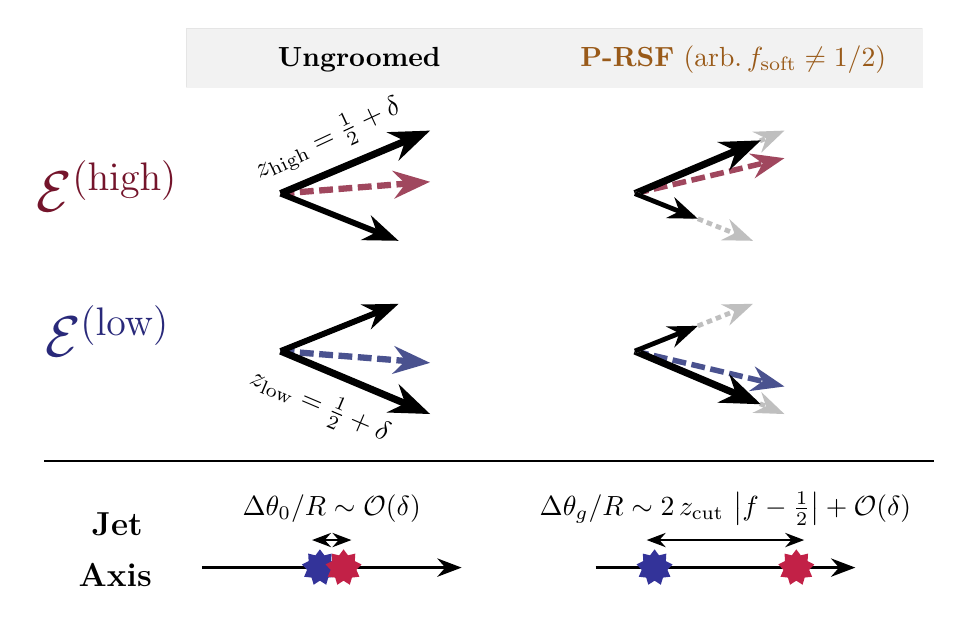
\begin{tikzpicture}[baseline=-3.5ex]

% Event Labels
  \node at (-1.7,  .6)()
        {\textcolor{black!40!E1color}{\huge \(\mathcal{E}^{(\rm high)}\)}};
  \node at (-1.7,  -1.25)()
         {\textcolor{black!20!E2color}{\huge\(\mathcal{E}^{(\rm low)}\)}};

% Header wrapper
\draw [fill=black, opacity=0.05]
       (-0.7,2.6) -- (8.65,2.6) -- (8.65,1.85) -- (-0.7,1.85) -- cycle;

%%%%%%%%%%%%%%
% Ungroomed
%%%%%%%%%%%%%%-
  \node at (1.5,  2.2)() {\textbf{Ungroomed}};

% E1
  % points
  \coordinate (O)  at (0.5, .5);
  \coordinate (A)  at (2.4, 1.3);
  \coordinate (B)  at (2.0, -0.1);
  \coordinate (M) at (2.4, 0.65);

  % legs
  \draw[-Stealth,line width=.8mm, color=aurometalsaurus!40!E1color, dash pattern=on 5pt off 2pt] (O) -> (M);
  \draw[-Stealth,line width=.9mm] (O) -> (A);
  \draw[-Stealth,line width=.75mm] (O) -> (B);

  % Descriptors
    \node [rotate=25] at (1.1,  1.2)()
        {\(z_{\rm high} = \frac{1}{2} + \delta\)};

% E2
  % points
  \coordinate (O)  at (0.5, -1.5);
  \coordinate (A)  at (2.4, -2.3);
  \coordinate (B)  at (2.0, -0.9);
  \coordinate (M) at (2.4, -1.65);

  % legs
  \draw[-Stealth,line width=.8mm, color=aurometalsaurus!40!E2color, dash pattern=on 5pt off 2pt] (O) -> (M);
  \draw[-Stealth,line width=.9mm] (O) -> (A);
  \draw[-Stealth,line width=.75mm] (O) -> (B);

  % Descriptors
    \node [rotate=-23] at (1.0,  -2.2)()
        {\(z_{\rm low} = \frac{1}{2} + \delta\)};

%%%%%%%%%%%%%%
% PIRANHA Grooming P-RSF
%%%%%%%%%%%%%%
  %\node at (6.25,  2.05)() {\textcolor{forestgreen(web)!75!black}{\textbf{RSF, \(f_{\rm soft} = 1\) (RSF\(_1\))}}};
  \node at (6.25,  2.2)() {\textcolor{ochre!75!black}{\textbf{P-RSF} (arb.\,\(f_{\rm soft}\neq 1/2\))}};

% E1
  % points
  \coordinate (O)  at (5.0, .5);
  \coordinate (A)  at (6.9, 1.3);
  \coordinate (Ap)  at (6.6, 1.176);
  \coordinate (B)  at (6.5, -0.1);
  \coordinate (Bp)  at (5.8, 0.18);
  \coordinate (M) at (6.9, 0.95);

  % legs
  \draw[-Stealth,line width=.7mm, color=aurometalsaurus!40!E1color, dash pattern=on 5pt off 2pt] (O) -> (M);
  \draw[-Stealth,line width=.6mm, dash pattern=on 2pt off 1.5pt, color=black!25!white] (O) -> (A);
  \draw[-Stealth,line width=.9mm] (O) -> (Ap);
  \draw[-Stealth,line width=.6mm, dash pattern=on 2pt off 1.5pt, color=black!25!white] (O) -> (B);
  \draw[-Stealth,line width=.6mm] (O) -> (Bp);

% E2
  % points
  \coordinate (O)  at (5.0, -1.5);
  \coordinate (A)  at (6.9, -2.3);
  \coordinate (Ap)  at (6.6, -2.176);
  \coordinate (B)  at (6.5, -0.9);
  \coordinate (Bp)  at (5.8, -1.18);
  \coordinate (M) at (6.9, -1.95);

  % legs
  \draw[-Stealth,line width=.7mm, color=aurometalsaurus!40!E2color, dash pattern=on 5pt off 2pt] (O) -> (M);s
  \draw[-Stealth,line width=.6mm, dash pattern=on 2pt off 1.5pt, color=black!25!white] (O) -> (A);
  \draw[-Stealth,line width=.9mm] (O) -> (Ap);
  \draw[-Stealth,line width=.6mm, dash pattern=on 2pt off 1.5pt, color=black!25!white] (O) -> (B);
  \draw[-Stealth,line width=.6mm] (O) -> (Bp);

%%%%%%%%%%%
% Dividing line
%%%%%%%%%%%
\coordinate (I)  at (-2.5, -2.9);
\coordinate (F)  at (8.8, -2.9);
\draw[line width=.3mm] (I) -> (F);

\node at (-1.575,  -3.7)()
        {\large \textbf{Jet}};
\node at (-1.6,  -4.35)()
        {\large \textbf{Axis}};

%%%%%%%%%%%%%%
% Jet Axis
%%%%%%%%%%%%%%
% Ungroomed
\coordinate (I)  at (-0.5, -4.25);
\coordinate (F)  at (2.8, -4.25);
\draw[-Stealth, line width=.45mm] (I) -> (F);

  % Events
  \node[star,star points=9,minimum width=.01cm,star point ratio=1.4,fill=E2color] at (1.0, -4.25) {};
  \node[star,star points=9,minimum width=.01cm,star point ratio=1.4,fill=E1color] at (1.3, -4.25) {};

  % Label
  \coordinate (I)  at (0.9, -3.9);
  \coordinate (F)  at (1.4, -3.9);
  \draw[Stealth-Stealth, line width=.3mm] (I) -> (F);
  \node at (1.15,  -3.5)()
        {\(\Delta\theta_0 / R \sim \mathcal O(\delta)\)};

% P-RSF
\coordinate (I)  at (4.5, -4.25);
\coordinate (F)  at (7.8, -4.25);
\draw[-Stealth, line width=.45mm] (I) -> (F);

  % Events
  \node[star,star points=9,minimum width=.01cm,star point ratio=1.4,fill=E2color] at (5.25, -4.25) {};
  \node[star,star points=9,minimum width=.01cm,star point ratio=1.4,fill=E1color] at (7.05, -4.25) {};

  % Label
  \coordinate (I)  at (5.15, -3.9);
  \coordinate (F)  at (7.15, -3.9);
  \draw[Stealth-Stealth, line width=.3mm] (I) -> (F);
  \node at (6.15,  -3.5)()
        {\(
          \Delta\theta_g / R
          \sim
          2\,\zcut\,\left|f - \frac{1}{2}\right|
          + \mathcal O(\delta)
        \)};

\end{tikzpicture}
}
\caption[A cartoon demonstrating the soft discontinuity of P-RSF for \(f_{\rm soft} \neq 1/2\) acting on toy jets.]{
A cartoon demonstrating the soft discontinuity of P-RSF for \(f_{\rm soft} \neq 1/2\) acting on the nearly identical events \(\mathcal E^{(\rm high, low)}\), each with two particles with nearly identical energy fractions, \(z \sim 1/2\), and with opening angle \(R\).
%
Red denotes the event \(\mathcal E^{(\rm high)}\), blue denotes \(\mathcal E^{(\rm low)}\), and a thick dotted arrow indicates the jet axis for each event.
%
The hardest particle of \(\mathcal E^{(\rm high)}\) is its upper particle, while the hardest particle of \(\mathcal E^{(\rm low)}\) is its lower particle.
%
Since P-RSF with \(f_{\rm soft} \neq 1/2\) preferentially subtracts radiation from the softer particle of each event, the events are mapped discontinuously to distinct groomed results.
%
The discontinuous behavior of the groomed jet axis is one manifestation of this soft discontinuous behavior:
%
while the ungroomed energy-weighted jet axes of \(\mathcal E^{(\rm high)}\) and \(\mathcal E^{(\rm low)}\) differ by an infinitesimal amount (\(\Delta\theta_0 \sim R \epsilon\)), the groomed jet axes are widely separated for any \(f_{\rm soft} \neq 1/2\).
}
\label{fig:rsf_discont}
\end{figure}

In the example of \Fig{rsf_discont}, we explore the effect of the soft discontinuity of Unbalanced P-RSF on the axis of a jet.
%
In particular, we examine nearly identical two-parton jets in the region of phase space near \(z \sim 1/2\) that differ only by an infinitesimally soft perturbation.
%
We denote these events by \(\mathcal{E}^{(i)}\), where \(i \in \{{\rm high, low}\}\).
%
The \(\mathcal E^{(i)}\) each consist of two particles: a ``high'' and ``low'' particle separated by an angular distance \(R\).
%
In \(\mathcal{E}^{(i)}\), particle \(i\) has just slightly more energy, \(z_i = 1/2 + \delta\).

For simplicity, we focus on the discontinuous behavior of the energy-weighted jet axis,
%
\begin{equation}
    \hat n_{\rm jet} \propto z_{\rm high} \hat n_{\rm high} +  z_{\rm low} \hat n_{\rm low}
    ,
\end{equation}
for the groomed events \(\mathcal E^{(i)}\), and the proportionality holds up to normalization.
%
Since the ungroomed \(\mathcal{E}^{(i)}\) are nearly identical, the angle between the ungroomed jet axes is infinitesimally small:
\begin{subequations}
\begin{align}
    \Delta\theta_{0}
   &=
    2\,R\,\delta
    +
    \mathcal{O}(R^3,\,\delta^3)
    ,
    \\
    \lim_{\delta\to 0}\Delta\theta_0 &= 0
    ,
\end{align}
\end{subequations}
where \(\Delta\theta_{0}\) indicates the angle between the jet axes of \(\mathcal{E}^{(\rm high)}\) and \(\mathcal{E}^{(\rm low)}\) before grooming.
%
After the application of P-RSF, however, the softer branch of each event will be dramatically diminished, and there is a large angle between the two groomed jet axes:
%
\begin{equation}
    \lim_{\delta\to 0}\Delta \theta_{g}
    =
    2\,R
    \,
    \frac{\zcut}{1 - \zcut}
    \,
    \left|f_{\rm soft} - 1/2\right|
    +
    \mathcal{O}(R^3)
    \neq 0
    \label{eq:prsf_soft_discont}
    ,
\end{equation}
where \(\Delta\theta_{g}\) indicates the angle between the jet axes of \(\mathcal{E}^{(\rm high)}\) and \(\mathcal{E}^{(\rm low)}\) after grooming with P-RSF.
%
The continuous behavior indicated by \(\lim_{\delta\to 0} \Delta\theta_0 = 0\) before grooming is in sharp contrast to the discontinuous behavior after grooming, \(\lim_{\delta\to 0} \Delta\theta_g \neq 0\).
%
In \Eq{prsf_soft_discont}, we have assumed that \(\max(f,\,1-f)\,\zcut < 1/2 - \delta\), so that neither particle is fully removed from the event.
%
Of course, when \(f_{\rm soft} = 1/2\), the grooming algorithm treats the harder and softer sub-jets equally, so that we once again have \(\Delta \theta_g \to \mathcal{O}(\delta)\) and the soft discontinuous behavior fades away.

This simple example demonstrates a general principle for designing Recursive Subtraction algorithms:
%
if they are to be soft-continuous, they must treat the softer and harder sub-jets identically in the limit \(z \to 1/2\).
%
For example, let us imagine a P-RSF--type grooming algorithm with \(f_{\rm soft}\) upgraded to a function of the energy fraction \(z\) and angle \(\theta\) of a branch, \(f_{\rm soft} \to f(z,\theta)\).
%
Any P-RSF-type groomer with \(f(1/2,\, \theta) = 1/2\) overcomes the soft discontinuity discussed of the discussion above.
%
We call such P-RS groomers that treat emissions in the region \(z = 1/2\) identically ``Hard-Balanced'' Recursive Subtractors, as they are balanced in the region of phase space where two sub-jets are equally hard.
%
A P-RSF algorithm with \(f(z, \theta) = 1 - z\), for example, is Hard-Balanced, and still preferentially grooms infinitesimally soft radiation.
%
We leave the study of Hard-Balanced Recursive Subtractors to future work.

Finally, we note that while the soft discontinuity we detailed above is an important formal feature of P-RSF, the regions of phase space where \(z \sim 1/2\) contribute far less to observable distributions than those for which \(z \sim \zcut\).
%
In particular, the pseudo-probability distribution for \(z\) scales as \(1/z\) in \gls{pqcd}, implying that the soft discontinuity of Unbalanced P-RSF that we explore above is suppressed relative to the soft discontinuities of hard-cutoff groomers such as Soft Drop.
%
Indeed, the soft discontinuities of P-RSF do not manifest in leading logarithmic substructure distributions, and we may even use P-RSF with \(f_{\rm soft} \neq 1/2\) to gain perturbative insight into the soft continuous analog, \PRSF{1/2}, and into \PIRANHA{} grooming in general, as discussed in \Sec{pira-resummed}.

On the other hand, soft discontinuities associated with hard cutoffs in traditional grooming procedures lie on the interior of the jet phase space, straddled by the regions \(0 < z < \zcut\) and \(\zcut < z < 1/2\).
%
As we saw in \Sec{sd_discont_lo}, the associated soft discontinuities lead to piece-wise definitions of groomed observable distributions even at \glslink{accuracy}{NLO} to isolate the behavior of radiation above and below the associated hard cutoff.

\subsection{Clustering Discontinuities in All Tree-Based Grooming}
\label{sec:ang_discont}

Recursive tree-based grooming algorithms also suffer from \textit{clustering discontinuities}, or discontinuities inherited from the procedure of clustering the jet into a tree of emissions (as discussed in \Sec{recursive-subtraction}).
%
Clustering discontinuities are inevitable in tree-based grooming because any clustering algorithm relies on the discontinuous notion of which particles are ``closest'' to one another.
%
However, since there is only one way to cluster a two-parton jet, clustering discontinuities only emerge beyond \glslink{accuracy}{NLO} and when a jet contains three or more partons.

Soft Drop and P-RSF in particular suffer from an \textit{angular clustering discontinuity}.
%
Both rely on an angular-ordered jet clustering history obtained from the angular-ordered C/A clustering algorithm;
%
the notion of the C/A clustering history is discontinuous because small changes to the angles of jet constituents may lead to distinct clustering histories.
%
Concretely, we say angular-ordered clustering algorithms and angular-ordered, tree-based grooming algorithms are angularly discontinuous in a measure zero region of phase space.

%-----------------------------------
% Angular Discontinuity Fig:
%-----------------------------------
\begin{figure}[t!]
      \centering
      \subfloat[]{
          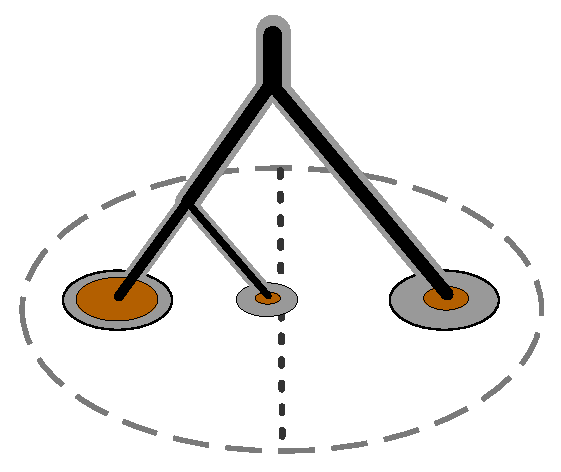
\includegraphics[width=.4\textwidth]{figures/piranha/cartoons/angular_discont_left}
          \label{fig:ang_discont_left}
      }
      ~~~~
      \subfloat[]{
          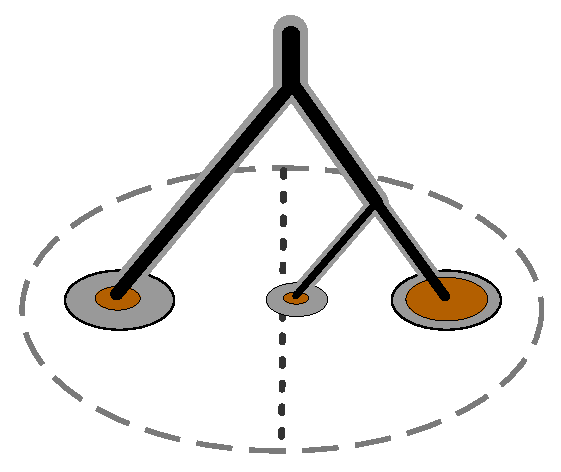
\includegraphics[width=.4\textwidth]{figures/piranha/cartoons/angular_discont_right}
          \label{fig:ang_discont_right}
      }
      \caption[A visualization of angular discontinuity in tree-based grooming.]{
    A visualization of angular discontinuity in tree-based grooming in the style of \Fig{rsf_tree}, with the angular-ordered \PRSF{1/2} algorithm as a representative example.
    %
    The thick dashed line in the center of the jet is equidistant in angle from the left and right sub-jets of the event, and the middle emission lies nearly on this line.
    %
    In (a), the middle emission lies closer to the left sub-jet, and the right sub-jet is therefore groomed more.
    %
    In (b), the middle emission is closer to the right sub-jet, and the left sub-jet is groomed more.
    %
    We see that a small change in the angle of the middle emission may drastically change the clustering history of the jet, and the result of a tree-based grooming procedure.
}
\label{fig:angdiscont}
\end{figure}


In our discussion, we focus on a simple manifestation of angular clustering discontinuities in the three-parton jet shown in \Fig{angdiscont}.
%
In particular, we consider the region of phase space where a particular sub-jet is nearly equidistant from a sub-jet on the left and another on the right.
%
We call the left and right sub-jets \(L\) and \(R\), and we denote the equidistant emission as \(M\), for ``middle''.

A small change in the location of emission \(M\) may lead to distinct C/A clustering histories.
%
If \(M\) is slightly closer to the left emission \(L\), then \(L\) will receive a quarter of the total grooming while \(R\) will receive half (as in \Fig{ang_discont_left});
%
the result is that \(L\) is groomed less than \(R\), and much more of the structure of the left side of the jet is preserved after the grooming.
%
Alternatively, if \(M\) is slightly closer to the right, then \(R\) will be groomed less than \(L\);
%
the right side of the jet will be preserved while much of the left side will be groomed away (as in \Fig{ang_discont_right}).
%
Despite the similarity of the ungroomed events, the resulting groomed events will have macroscopic differences and be separated by a relatively large EMD.

To emphasize this point quantitatively, let us consider P-RSF acting on the simple example where all three emissions lie in a plane, the left and right emissions each have an energy fraction \(z_\ell = z_r = z_0\), and the middle emission -- nearly equidistant from the left and right emissions -- has \(z_m = 1-2z_0\).\footnote{We focus on P-RSF in this example to avoid the more complex analysis required for Soft Drop that may obfuscate the physics at hand.
%
Soft Drop also exhibits an angular clustering discontinuity that can be seen in the context of this simple example, but that is complicated by the possible behaviors of the grooming:
%
\(\zcut\) and \(z_0\) may conspire such that zero, one, or two emissions are groomed from the event.
%
The effects of the clustering discontinuity on the energy-weighted jet axis must therefore be considered piece-wise in the \((\zcut,\,z_0)\) parameter space.
}
%
We use \(R\) to denote the angle between the left and right emissions, and \(\delta\) to denote a small perturbation in the angle of the middle emission:
%
\(\theta_{\ell m} = R/2 + \delta\) in one event, while \(\theta_{\ell m} = R/2 - \delta\) in the other.
%
We again examine the discontinuity in the energy-weighted jet axis, which takes the more general form
\begin{align}
    \hat{n}_{\rm jet} \propto \sum_i z_i \hat{n}_i
    ,
\end{align}
where the proportionality holds up to normalization.
%
A simple computation then yields
\begin{subequations}
\begin{align}
    \Delta\theta_0
    &=
    2\, z_m \, \delta
    +
    \mathcal{O}\left(R^2, \delta^3\right)
    ,
    \\
    \lim_{\delta\to 0}\Delta\theta_0 &= 0
    ,
\end{align}
\end{subequations}
for the angle \(\Delta\theta_0\) between the two jet axes before grooming, while
\begin{align}
    \lim_{\delta\to 0}\Delta\theta_g
    &=
    R\,\frac{\zcut}{1-\zcut}\,\left|f(f-3)+1\right|
    +
    \mathcal{O}(R^3)
    \neq 0
    ,
\end{align}
for the angle between the two jet axes after the application of P-RSF, where we have assumed that \(\zcut\) is sufficiently small that all particles survive the grooming.
%
We again see a discontinuous behavior in the energy-weighted axis of the groomed jets, \(\lim_{\delta\to 0}\Delta\theta_g \neq 0\), despite the fact that the ungroomed events were nearly identical and \(\lim_{\delta\to 0}\Delta\theta_0 = 0\).


Fortunately, the angular discontinuities associated with tree-based clustering algorithms are also suppressed in the phase space of \gls{pqcd}.
%
First, we note that the angular discontinuities in angular-ordered clustering algorithms emerge only at higher orders of perturbative accuracy for which a jet has three or more constituents.
%
These regions of phase space are generically suppressed in high-energy QCD calculations, where the emission of extra final-state partons is suppressed by the strong coupling constant \(\alpha_s\).
%
Furthermore, \gls{pqcd} predicts a strong hierarchy in the angles between different emissions in a jet, \(\theta_1 \gg \theta_2 \gg \cdots\) \cite{Collins:2011zzd}.
%
Therefore, even among phase space configurations with three or more constituents, it is very unlikely in \gls{pqcd} to find a configuration in which a particular final-state particle lies nearly equidistant in angle between two others.

We also emphasize that the angular discontinuity of the C/A clustering algorithm is representative of more general discontinuities in tree-based clustering and in jet algorithms.\footnote{
To mitigate the discontinuities of tree-based clustering, one can introduce a continuous weighting procedure for clustering histories.
%
One way to assign continuous weights to different clustering histories is the \textsc{Q-jet} scheme \cite{Ellis:2012sn,Ellis:2014eya}, which notably leads to reduced statistical fluctuations in observable distributions compared to the standard scheme of using a single clustering history for jet substructure calculations.
%
While the \textsc{Q-jet} scheme has not been applied directly to grooming in the context of energy flows, to our knowledge, it provides a particularly simple way to overcome the clustering discontinuities we discuss here:
%
we may simply define an overall groomed energy flow -- devoid of clustering discontinuities -- as the weighted average of the groomed energy flows associated with each possible clustering history.
}
%
For example, the \(k_t\) and anti-\(k_t\) algorithms exhibit a similar \(k_t\) discontinuity by identical arguments.
%
Discontinuities of different clustering algorithms may be more or less suppressed in the phase space of \gls{pqcd}, or more or less sensitive to particular sources of low-energy pollution.
%
Therefore, a more detailed discussion of clustering discontinuities and re-clustering schemes that minimize their effects is a potential direction for future research.


%==============================================
\section{Groomed Jet Phenomenology}
%==============================================
\label{sec:grooming-pheno}

We now demonstrate the soft insensitivity enjoyed by \PIRANHA{} groomers over hard-cutoff groomers through several phenomenological studies.
%
In \Secs{pira-hadronization}{pira-neutral}, we compare the responses of the hard-cutoff Soft Drop algorithm and \PRSF{1/2} to \glspl{soft-distortion} from \gls{hadronization} and to the removal of neutral particles, as a proxy for \gls{deteffects}.
%
In \Secss{pira-pu}{pira-ue}{pira-mass}, we compare the ability of Soft Drop and \PRSF{1/2} to effectively remove \gls{additive-contamination} from \gls{pileup} and \gls{ue}, which both consist of \textit{extra} soft radiation that sits on top of a hard process.
%
In particular,
\begin{itemize}
    \item
        We use \PRSF{1/2} as a representative of \PIRANHA{} grooming procedures;

    \item
        We use Soft Drop with \(\beta_{\rm SD} = 2\) as a representative of traditional grooming procedures.

    \item
        In our \gls{pileup} studies, we use Constituent Subtraction (CS), a constituent-level area subtraction method for \gls{pu-mitigation} \cite{Berta:2014eza}, as a representative of \gls{pileup} mitigation procedures.
\end{itemize}
%
We also present more detailed phenomenological comparisons of \PIRANHA{} and \glslink{hard-cutoff-groomer}{hard-cutoff grooming algorithms} in \App{feedingfrenzy}


The case of \gls{additive-contamination} is qualitatively different than that of \glspl{soft-distortion};
%
we do not want to examine the robustness of the grooming procedure to \gls{additive-contamination}, but rather the ability of the grooming to \textit{remove} the contamination.
%
In our \gls{pileup} mitigation studies, we find that \PRSF{1/2} -- which behaves comparably to CS -- is a more effective tool than \SD{2}.
%
In our \gls{ue} studies, we find that \PRSF{1/2} and \SD{2} are comparable tools for the subtraction of \gls{ue} effects from jet substructure.

We simulate \gls{pileup} using the dijet and minimum bias samples from \Reff{Soyez:2018opl}, produced using \texttt{Pythia 8.185} with tune 4C for proton-proton collisions at \(\sqrt{s}\) = 14 TeV.
%
We layer minimum bias events on top of the hard dijet events, taking the number of \glslink{pileup}{pileup} events to be Poisson distributed with a mean of \(\langle n_{\rm PU}\rangle\) = 50 events.

We simulate \gls{ue} by turning on multiple parton interactions in \texttt{Pythia 8.244} \cite{Sjostrand:2014zea} with the default Monash tune \cite{Skands:2014pea}.
%
We begin with a study of QCD jets and, to roughly echo similar studies in the original Soft Drop paper \cite{Larkoski:2014wba}, also explore the groomed mass resolution of jets produced by boosted \(W\) bosons and top quarks in the presence of \gls{ue}.

For details regarding other \PIRANHA{} grooming procedures and Soft Drop with different \(\beta_{\rm SD}\), see \App{feedingfrenzy}.




%=====================================
% Hadronization:
%=====================================
\subsection{Hadronization Response}
\label{sec:pira-hadronization}

We first provide phenomenological evidence that continuous grooming is less sensitive than hard-cutoff grooming to the physics of \gls{hadronization}.
%
A deep understanding of the physics of traditional jets requires careful consideration of \gls{hadronization} corrections, such as in jet masses \cite{Hoang:2019ceu, Marzani:2017kqd, Benkendorfer:2021unv} and hadronic event shapes \cite{Dokshitzer:1995zt, Baron:2020xoi}.
% and we hope that \PIRANHA{} grooming provides observables that may be more easily understood without complicated non-perturbative input.
%
Hard-cutoff groomed jet observables in particular can undergo large corrections from the \gls{hadronization} process due to the discontinuity of the hard-cutoff paradigm:
%
\gls{hadronization} can transform partons with energy below a hard cutoff into hadrons with energy above the hard cutoff, and vice versa.
%
These subtleties lead to additional complications in the theoretical calculation of non-perturbative effects on traditionally groomed jet observables \cite{Hoang:2019ceu}.

%-----------------------------------
% Parton-Hadron EMD:
%-----------------------------------
\begin{figure}[p]
\centering
\subfloat[][]{
      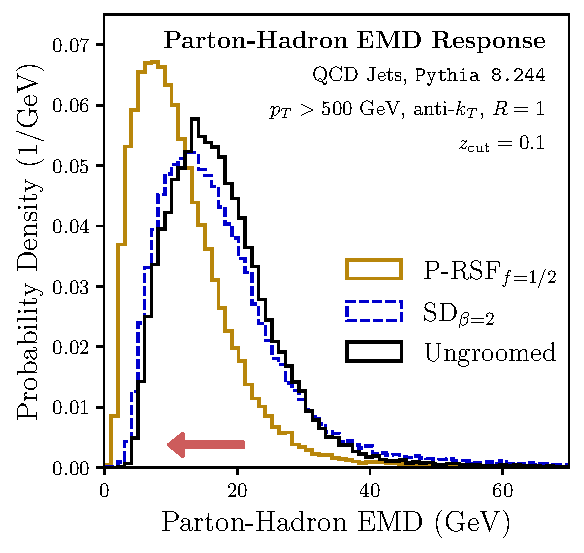
\includegraphics[width=.32\textwidth]
      {figures/piranha/responses/pvh/emd_dist-ph}
      \label{fig:ph_emd_dist}
}
\subfloat[][]{
      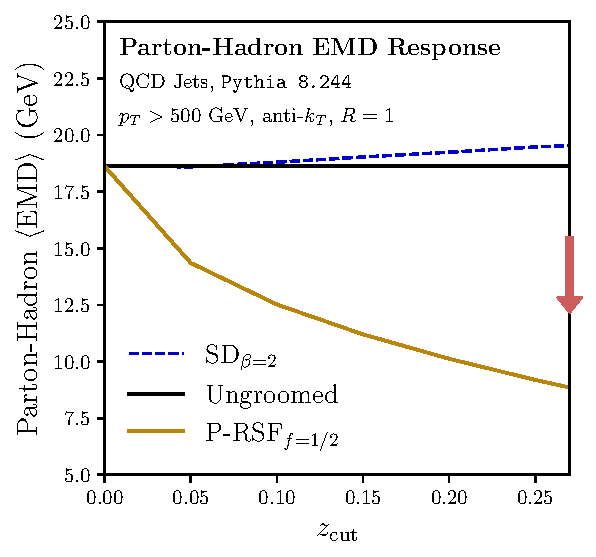
\includegraphics[width=.32\textwidth]
      {figures/piranha/responses/pvh/deltaemd-ph}
      \label{fig:ph_emd_delta}
}
\subfloat[][]{
      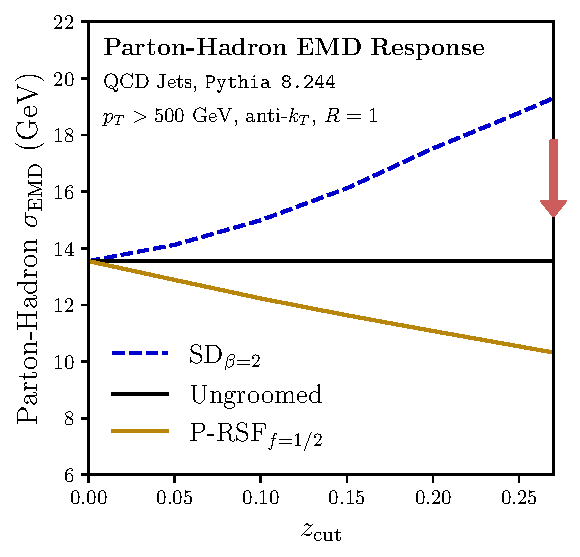
\includegraphics[width=.32\textwidth]
      {figures/piranha/responses/pvh/sigmaemd-ph}
      \label{fig:ph_emd_sigma}
}
\\
\subfloat[][]{
      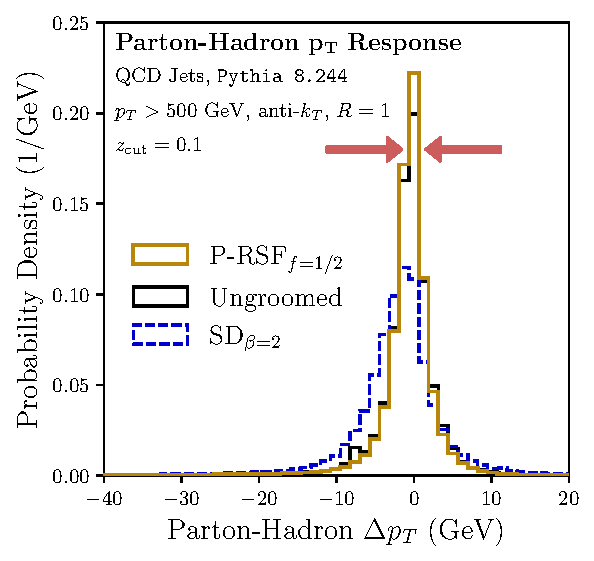
\includegraphics[width=.32\textwidth]
      {figures/piranha/responses/pvh/delta_pt_dist-ph}
      \label{fig:ph_pt_dist}
}
\subfloat[][]{
      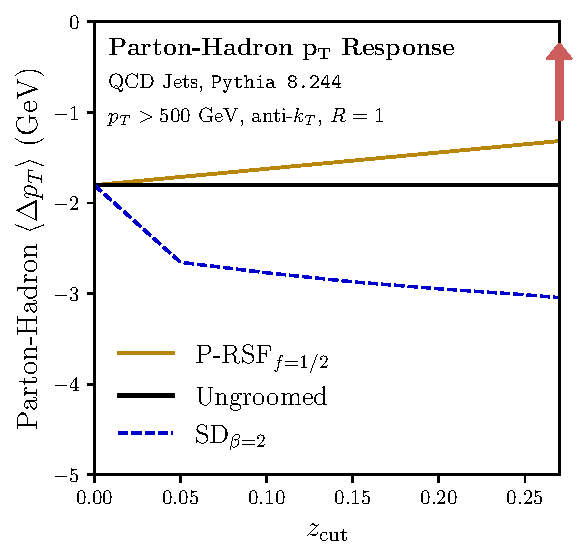
\includegraphics[width=.32\textwidth]
      {figures/piranha/responses/pvh/deltapt-ph}
      \label{fig:ph_pt_delta}
}
\subfloat[][]{
      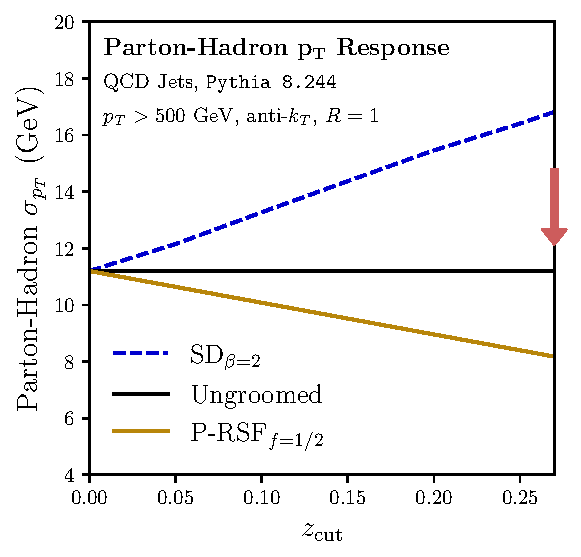
\includegraphics[width=.32\textwidth]
      {figures/piranha/responses/pvh/sigmapt-ph}
      \label{fig:ph_pt_sigma}
}
\\
\subfloat[][]{
      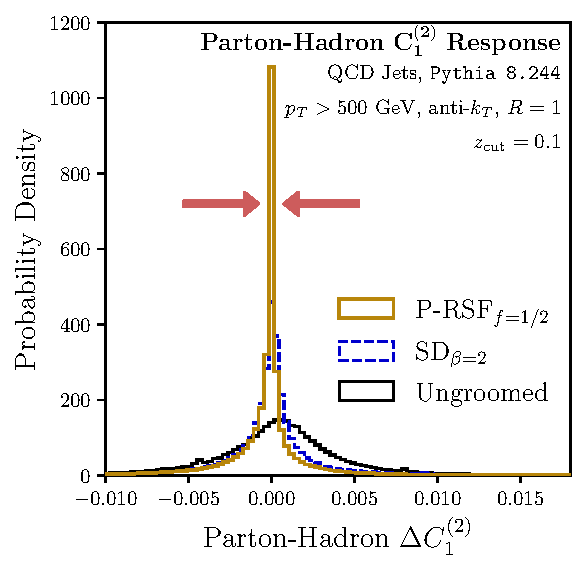
\includegraphics[width=.32\textwidth]
      {figures/piranha/responses/pvh/deltac12_dist-ph}
      \label{fig:ph_c12_dist}
}
\subfloat[][]{
      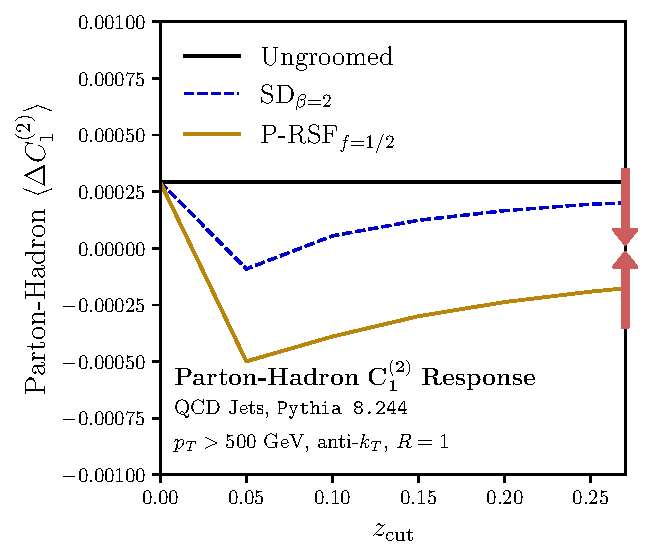
\includegraphics[width=.32\textwidth]
      {figures/piranha/responses/pvh/deltac12-ph}
      \label{fig:ph_c12_delta}
}\subfloat[][]{
      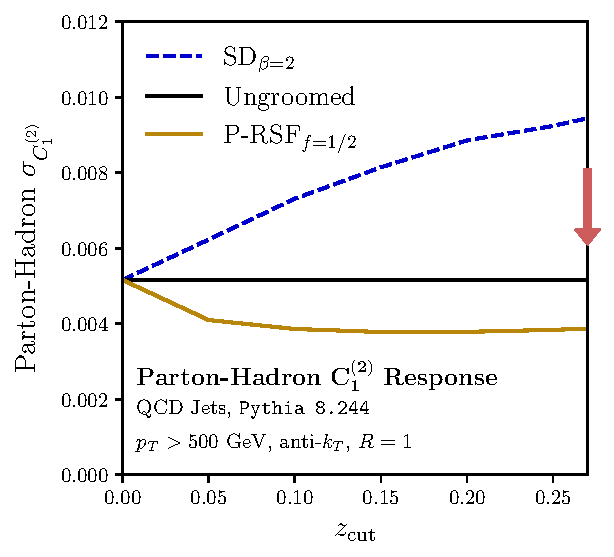
\includegraphics[width=.32\textwidth]
      {figures/piranha/responses/pvh/sigmac12-ph}
      \label{fig:ph_c12_sigma}
}
    \caption[Per-jet hadronization responses of the EMD, \(\Delta p_T\), and \(\Delta C_1^{(2)}\) using Balanced Recursive Subtraction and Soft Drop with \(\beta_{\rm SD} = 2\).]{
        Per-jet \gls{hadronization} responses of (top row) EMD, (middle row) \(\Delta p_T\), and (bottom row) \(\Delta C_1^{(2)}\) using Balanced Recursive Subtraction (\PRSF{1/2}, orange) and Soft Drop with \(\beta_{\rm SD} = 2\) (\SD{2}, blue).
        %
        We display (left column) the distribution of the response for \zcut=0.1, (middle column) the mean response as a function of \zcut, and (right column) the standard deviation of the response as a function of \zcut.
    %
    The red arrows indicate the direction corresponding to better performance.
    }
\label{fig:parton_hadron_response}
\end{figure}

In \Fig{parton_hadron_response}, we compare how ungroomed jets, traditionally groomed jets, and \PIRANHA{}-groomed jets respond to \gls{hadronization} in the context of energy flow, extensive properties, and substructure.
%
Our studies focus on the parton-hadron EMD (the EMD between parton-level jets and their hadron-level counterparts), the parton-hadron \(\Delta p_T\), and the parton-hadron \(\Delta C_1^{(2)}\).
%
\PIRANHA{}-groomed jets typically exhibit smaller and more predictable responses to \gls{hadronization}, evinced by the reduced variance in their \gls{hadronization} response.
%
One key factor in the improved responses of \PIRANHA{}-groomed jets is the scaling-down of distortions due to \gls{hadronization} in \PIRANHA{}-groomed jets:
%
the subtractive approach of \PIRANHA{} (and in particular P-RSF when \(f_{\rm soft} \neq 0, 1\)) removes energy from every particle in the event, resulting in a controlled and uniform \gls{hadronization} response.
%
On the other hand, Soft Drop grooming does not implement continuous, event-wide subtraction.
%
Jets groomed with Soft Drop either retain or remove particles as a result of distortions due to \gls{hadronization}, resulting in a larger variance in the properties of jets groomed with Soft Drop.

We plot distributions of the parton-hadron EMD for groomed QCD jets for the benchmark value of $\zcut{}=0.1$ in \Fig{ph_emd_dist}.
%
We see a sharper peak at a smaller EMD in the parton-hadron EMD distributions for \PRSF{1/2} and longer tails for Soft Drop, already indicating that \gls{hadronization} is more likely to dramatically change the result of Soft Drop.
%
\Figs{ph_emd_delta}{ph_emd_sigma} show that the average parton-hadron EMD and the variance in the parton-hadron EMD are both smaller for \PRSF{1/2} groomed jets than for Soft Drop groomed jets for a wide range of \zcut{} values, again evincing that \PIRANHA{}-groomed jets have less sensitive responses to \gls{hadronization}.


The extensive observable \(p_T\) and the substructure observable \(C_1^{(2)}\) also reflect the increased robustness of \PIRANHA{}-groomed jets to \gls{hadronization}.
%
In our discussion of \gls{hadronization}, we characterize the response of \(p_T\) by using \Eq{pt_response} with \(p_T = p_T^{\rm(parton)}\) indicating the parton-level transverse momentum, before the addition of model-dependent \gls{hadronization} effects, and \(\widetilde{p_T} = p_T^{\rm(hadron)}\).
%
In \Fig{ph_pt_dist}, we see that for \(\zcut = 0.1\), \PIRANHA{}-groomed \(p_T\) again tends to have a sharper response to \gls{hadronization}, while \Figs{ph_pt_delta}{ph_pt_sigma} indicates that this sharper response holds for a wide range of \zcut{} values.
%
The behavior of the \(p_T\) closely mimics that of the parton-hadron EMD, evincing our arguments that the parton-hadron EMD provides a probe of generic jet observables to \gls{hadronization}.
%
In \Figss{ph_c12_dist}{ph_c12_delta}{ph_c12_sigma}, we make similar conclusions for \(C_1^{(2)} \approx m^2 / p_T^2\).
%
We first note that the parton-hadron shift in the \(C_1^{(2)}\) substructure observable is larger for \PRSF{1/2}, at least for fixed \zcut{}, and the substructure of \PRSF{1/2} groomed jets may undergo larger changes due to \gls{hadronization} than that of Soft Drop groomed jets.
%
However, the variance in the shift in \PRSF{1/2} groomed substructure is smaller than that of Soft Drop, indicating that the response of \PIRANHA{}-groomed substructure to \gls{hadronization} is more predictable than that of Soft Drop.

Overall, we find that \PIRANHA{}-groomed jets have more predictable responses to \gls{hadronization} than traditionally groomed jets, supported by the observable independent EMD, as well as by extensive observables and jet substructure.
%
We have provided evidence that IRC-safe observables of jets groomed with Soft Drop have generically larger responses to \gls{hadronization}, while \PIRANHA{}-groomed observables are generally less affected by the physics of \gls{hadronization}.
%
We hope that the stability of \PIRANHA{}-groomed jets to the non-perturbative physics of \gls{hadronization} may facilitate even further communication between theoretical predictions and experimental results for groomed jet observables.

%=====================================
% All vs. Charged:
%=====================================
\subsection{All Versus Charged}
\label{sec:pira-neutral}

%-----------------------------------
% All-Charged EMD:
%-----------------------------------
\begin{figure}[p]
    \subfloat[][]{
          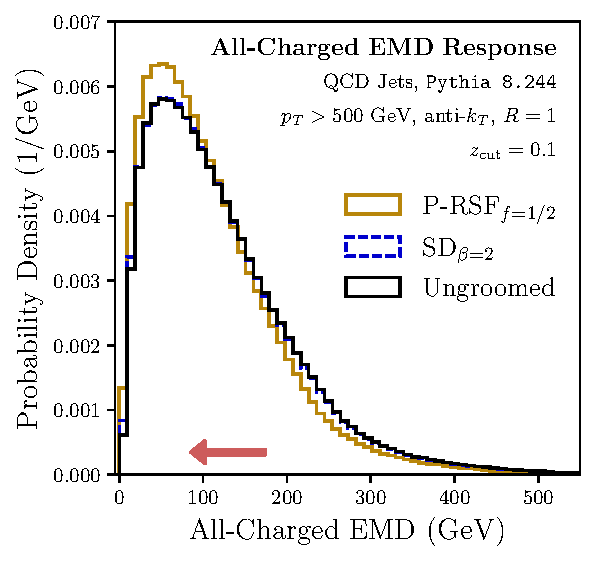
\includegraphics[width=.32\textwidth]
          {figures/piranha/responses/avc/emd_dist-avc}
          \label{fig:avc_emd_dist}
    }
    \subfloat[][]{
          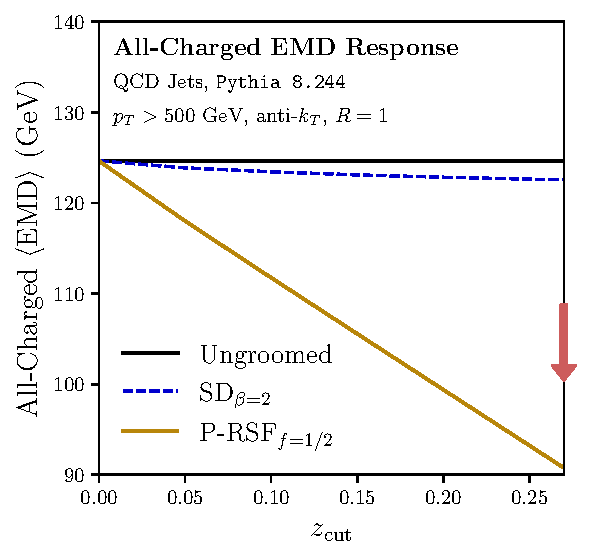
\includegraphics[width=.32\textwidth]
          {figures/piranha/responses/avc/deltaemd-avc}
          \label{fig:avc_emd_delta}
    }
    \subfloat[][]{
          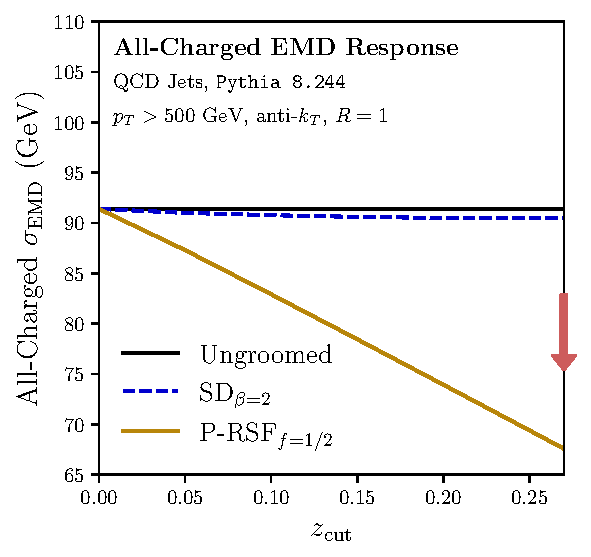
\includegraphics[width=.32\textwidth]
          {figures/piranha/responses/avc/sigmaemd-avc}
          \label{fig:avc_emd_sigma}
    }
    \\
    \subfloat[][]{
          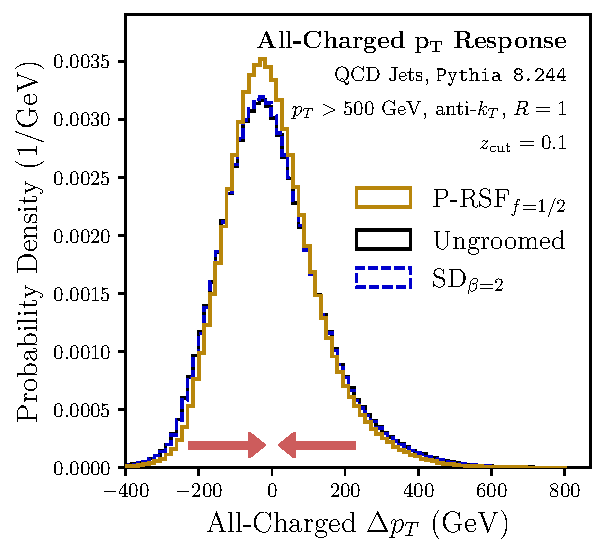
\includegraphics[width=.32\textwidth]
          {figures/piranha/responses/avc/delta_pt_dist-avc}
          \label{fig:avc_pt_dist}
    }
    \subfloat[][]{
          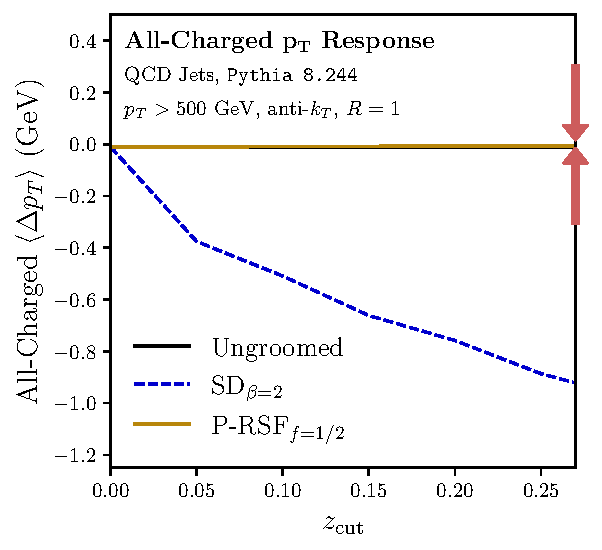
\includegraphics[width=.32\textwidth]
          {figures/piranha/responses/avc/deltapt-avc}
          \label{fig:avc_pt_delta}
    }
    \subfloat[][]{
          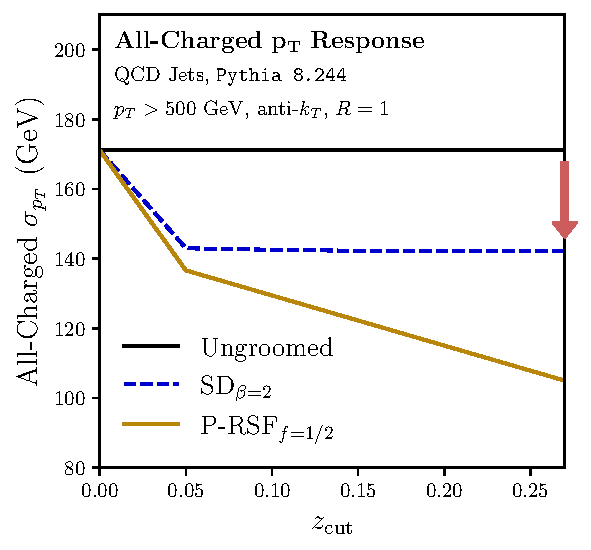
\includegraphics[width=.32\textwidth]
          {figures/piranha/responses/avc/sigmapt-avc}
          \label{fig:avc_pt_sigma}
    }
    \\
    \subfloat[][]{
          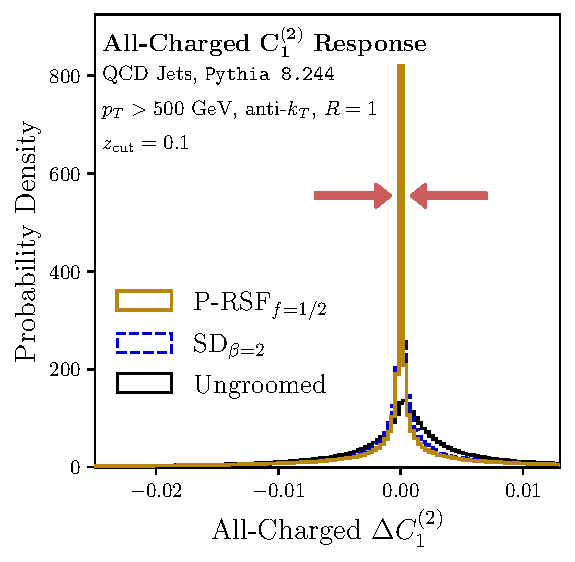
\includegraphics[width=.32\textwidth]
          {figures/piranha/responses/avc/deltac12_dist-avc}
          \label{fig:avc_c12_dist}
    }
    \subfloat[][]{
          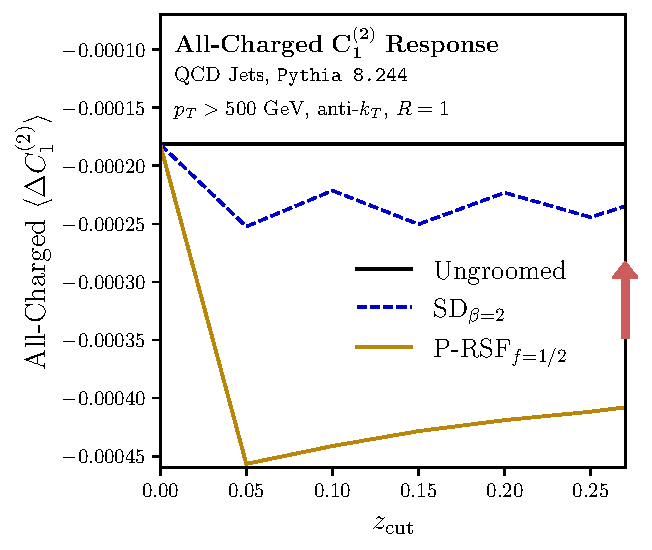
\includegraphics[width=.32\textwidth]
          {figures/piranha/responses/avc/deltac12-avc}
          \label{fig:avc_c12_delta}
    }
    \subfloat[][]{
          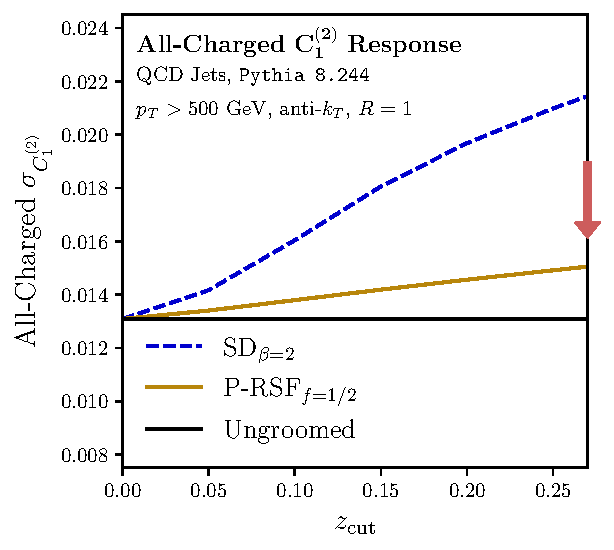
\includegraphics[width=.32\textwidth]
          {figures/piranha/responses/avc/sigmac12-avc}
          \label{fig:avc_c12_sigma}
    }
\caption[Responses to the exclusion of neutral particles of the EMD, \(\Delta p_T\), and \(\Delta C_1^{(2)}\) using Balanced Recursive Subtraction and Soft Drop with \(\beta_{\rm SD} = 2\).]{
    Same as \Fig{parton_hadron_response}, but for per-jet responses to the exclusion of neutral particles.
    %
    We rescale the \(p_T\) of the charged particles in order to eliminate the leading $p_T$ bias due to the loss of neutral energy.
}
\centering
\label{fig:avc_response}
\end{figure}

We next compare the response of hard-cutoff and \PIRANHA{} grooming to the exclusion of neutral particles, as a rough analog of the smearing of neutral particles due to \gls{deteffects}.
%
Small tweaks in experimental signatures due to \gls{deteffects} may produce large changes in hard-cutoff groomed observables, providing another obstacle in extracting fundamental physics from traditionally groomed jets.
%
The continuity of \PIRANHA{} again leads us to expect that \PIRANHA{}-groomed observables are more robust to \gls{deteffects} than traditionally groomed jet observables.


To counteract the leading bias due to the loss of neutral energy in the jet, we apply a rescaling to the \(p_T\) of the charged-only jet constituents:
%
\begin{align}
    \tilde p_T^i =
    \begin{cases}
        0,
        &\text{particle }i\text{ is neutral}
        \\
        p_T^i
        \frac{\left\langle p_T^\text{(all)}\right\rangle}{\left\langle p_T^\text{(charged)}\right\rangle},
        &\text{particle }i\text{ is charged}
    \end{cases}
    ,
    \label{eq:all-charged_rescaling}
\end{align}
where \(p_T^i\) is the transverse momentum of particle \(i\) in the original jet, \(\mathcal{J}\), containing both charged and neutral particles, and \(\tilde p_T^i\) is the transverse momentum we assign to particle \(i\) in the charged-only, rescaled jet, \(\tilde{\mathcal{J}}\), with neutral particles excluded.
%
Here, \(p_T^{\rm(all)} = \sum_i p_T^i\) is the total transverse momentum including both charged and neutral particles, while \(p_T^{\rm(charged)} = \sum_{i\text{ charged}} p_T^i\) includes only charged constituents.
%
The rescaling factor \(\big\langle p_T^\text{(all)}\big\rangle/\big\langle p_T^\text{(charged)}\big\rangle\)\(\approx\)\(1.47\) is defined such that the average $p_T$ is preserved after removing neutral particles.%
\footnote{
We can gain intuition for this rescaling factor by considering the isospin-preserving limit, where we expect similar numbers of \(\pi^+\), \(\pi^-\), and \(\pi^0\) mesons to be produced.
%
Events for which we discard the \(\pi^0\) particles should have roughly \(2/3\) the total transverse momentum, ignoring subtleties associated with kaons and other heavier states.
%
This leads to an estimate of \(\big\langle p_T^\text{(all)}\big\rangle/\big\langle p_T^\text{(charged)}\big\rangle \approx 3/2\) -- remarkably close to the numerical value of 1.47 found in \texttt{Pythia 8.244}.
}

In our discussion of EMD, we compute the response \(\text{EMD}\left(G(\mathcal{J}), G(\tilde{\mathcal{J}})\right)\), where \(G\) indicates the grooming algorithm under consideration;
%
we call this the \textit{all-charged EMD}.
%
Similarly, in our discussion of \Eq{pt_response}, we take \(p_T = p_T^{\rm(all)}\) to be the transverse momentum including both charged and neutral particles and \(\widetilde{p_T} = \sum_i \tilde p_T^i = p_T^{\text{(charged, rescaled)}}\) to be the rescaled contribution from charged particles only.
%
We refer to the difference as the all-charged \(p_T\) shift, or the all-charged \(\Delta p_T\).
%
Note that the rescaling procedure does not impact dimensionless charged-only substructure observables like \(C_1^{(2)}\), since they are normalized by the jet momentum.


Our comparison of the all-charged response of \PIRANHA{} grooming to that of traditional grooming procedures is shown in \Fig{avc_response}.
%
As in our study of \gls{hadronization}, we begin our study with a discussion of the EMD.
%
The all-charged EMD bounds changes in IRC-safe observables due to the exclusion of neutral particles and corresponding rescaling of charged particles.
%
Since neutral particles are the most susceptible to smearing effects due to detector responses, the all-charged EMD furnishes an observable-independent probe for the effects of experimental detectors on groomed jets.
%
We demonstrate distributions of the all-charged EMD for groomed QCD jets with several choices of grooming in \Fig{avc_emd_dist}.
%
The contrast between \PIRANHA{} and traditionally groomed all-charged EMD is not as sharp as for the parton-hadron EMD.
%
However, \PIRANHA{} grooming again enjoys smaller and more sharply peaked EMD responses to the exclusion of neutral particles.
%
\Fig{avc_emd_delta} shows that the all-charged EMD is smaller for P-RSF\(_{1/2}\) groomed jets than for Soft Drop groomed jets for a wide range of \zcut{} values.
%
\Fig{avc_emd_sigma} shows that the fluctuations in the all-charged EMD, and therefore the fluctuations in the response of grooming to our naive model of smearing, are noticeably smaller for \PIRANHA{} groomers than for traditional groomers.

Our results for the all-charged \(p_T\) shifts are similar to our results for the all-charged EMD.
%
\Fig{avc_pt_dist} demonstrates that the \(p_T\) response of \PRSF{1/2} is smaller and more sharply peaked for $\zcut = 0.1$, while \Figs{avc_pt_delta}{avc_pt_sigma} respectively show that the \PRSF{1/2} all-charged response remains small and sharply peaked for a wide range of \zcut{} values.
%
Indeed, the fluctuations of the all-charged \(p_T\) response are nearly identical for each \PIRANHA{} groomer.

\Figss{avc_c12_dist}{avc_c12_delta}{avc_c12_sigma} compare the robustness of \PRSF{1/2} and Soft Drop for the substructure observable \(C_1^{(2)}\).
%
\Fig{avc_c12_dist} again shows that the all-charged response of \PRSF{1/2} is more sharply peaked than that of Soft Drop.
%
Similarly, \Figs{avc_c12_delta}{avc_c12_sigma} demonstrate that the all-charged shifts to \PIRANHA{}-groomed jet substructure are generally larger but more predictable than those of Soft Drop for a wide range of \zcut{} values.
%
The increased robustness of \PIRANHA{} grooming procedures compared to Soft Drop is less sharp than in the case of \gls{hadronization}, but the \PIRANHA{}-groomed observables nonetheless have less spread and a stronger linear correlation in response to our naive model of smearing.


%=====================================
% Pileup:
%=====================================
\subsection{Minimum Bias Events and Pileup Response}
\label{sec:pira-pu}

%-----------------------------------
% Pileup:
%-----------------------------------
\begin{figure}[p]
\centerline{
\subfloat[][]{
      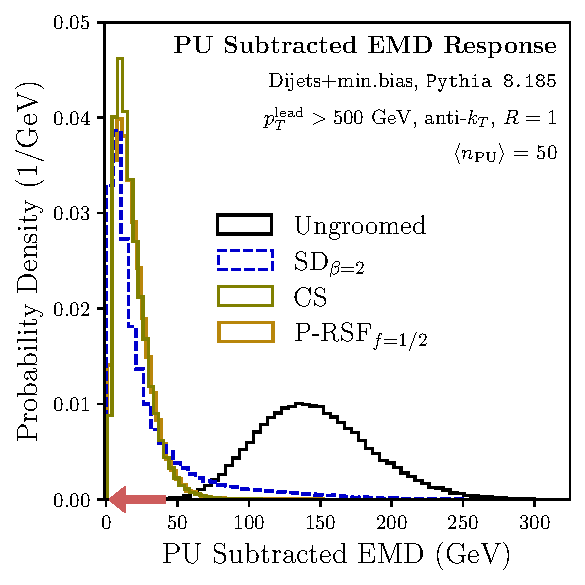
\includegraphics[width=.32\textwidth]{figures/piranha/responses/pileup/main_emd_npu50}
      \label{fig:pu_emd_dist}
}
\subfloat[][]{
      \includegraphics[width=.32\textwidth]{figures/piranha/responses/pileup/main_emd_npu_shifts}
      \label{fig:pu_emd_shift}
}
\subfloat[][]{
      \includegraphics[width=.32\textwidth]{figures/piranha/responses/pileup/main_emd_npu_stds}
      \label{fig:pu_emd_std}
}
} % centerline
~\\
\centerline{
\subfloat[][]{
      \includegraphics[width=.32\textwidth]{figures/piranha/responses/pileup/main_dpt_npu50}
      \label{fig:pu_pt_dist}
}
\subfloat[][]{
      \includegraphics[width=.32\textwidth]{figures/piranha/responses/pileup/main_dpt_npu_shifts}
      \label{fig:pu_pt_shift}
}
\subfloat[][]{
      \includegraphics[width=.32\textwidth]{figures/piranha/responses/pileup/main_dpt_npu_stds}
      \label{fig:pu_pt_std}
}
} % centerline
~\\
\centerline{
\subfloat[][]{
      \includegraphics[width=.32\textwidth]
      {figures/piranha/responses/pileup/main_dc1_npu50}
      \label{fig:pu_c12_dist}
}
\subfloat[][]{
      \includegraphics[width=.32\textwidth]
      {figures/piranha/responses/pileup/main_dc1_npu_shifts}
      \label{fig:pu_c12_shift}
}
\subfloat[][]{
      \includegraphics[width=.32\textwidth]
      {figures/piranha/responses/pileup/main_dc1_npu_stds}
      \label{fig:pu_c12_std}
}
} % centerline
\caption[Pileup-subtracted properties of the EMD, \(\Delta p_T\), and \(\Delta C_1^{(2)}\) using Balanced Recursive Subtraction and Soft Drop with \(\beta_{\rm SD} = 2\).]{
    Properties of per-jet \gls{pileup}-subtracted (top row) EMD, (middle row) \(\Delta p_T\), and (bottom row) \(\Delta C_1^{(2)}\), discussed in \Sec{pira-pu} for Balanced Recursive Subtraction (\PRSF{1/2}, orange), Soft Drop with \(\beta_{\rm SD} = 2\) (\SD{2}, blue), and Constituent Area Subtraction (CS, green).
    %
    We display (left column) the distribution of the each \gls{pileup}-subtracted observable for \(\langle n_{\rm PU}\rangle = 50\), (middle column) the mean \gls{pileup}-induced shift in each observable as a function of \(\langle n_{\rm PU}\rangle\), and (right column) the standard deviation of the \gls{pileup}-induced shifts in each observable as a function of \(\langle n_{\rm PU}\rangle\).
    %
    The red arrows indicate the direction corresponding to better performance.
}
\label{fig:pu_response}
\centering
\end{figure}

We first examine the effectiveness of different groomers in mitigating the effects of \gls{pileup} on the dijet events of \Reff{Soyez:2018opl}.
%
To quantify the ability of different groomers to remove \gls{pileup}, we perform an event-by-event comparison of \textit{hard events} to the associated \vocab{\glspl{pusubevent}}:
\begin{itemize}
    \item
    A \vocab{hard event} is a dijet event without any \gls{pileup}, representing the physics of a hard process;

    \item
    A \vocab{\gls{pusubevent}} is produced by simulating the \gls{additive-contamination} due to \gls{pileup} on top of a hard event and then attempting to groom the \gls{pileup} away.
\end{itemize}
%
To produce a \gls{pileup}-subtracted event, we first simulate \gls{pileup} by adding the energy distributions of a Poisson-distributed number of minimum bias events to the energy distribution of a given hard event.
    %
    We then estimate the contaminating energy density due to \gls{pileup} using the \texttt{GridMedianBackgroundEstimator} (GMBE) method of \texttt{FastJet} \cite{Cacciari:2011ma}.
    %
    We tune an additional correction factor that scales our estimate \(\rho_{\rm est.}\) relative to the GMBE value \(\rho_{\rm GMBE}\) for each grooming algorithm to subtract \glslink{pileup}{pileup} more effectively, as discussed in more detail in \App{feedingfrenzy}.
    %
    Finally, we produce the \gls{pusubevent} by removing a fraction \(\zcut\) of the jet \(p_T\) consistent with the estimated \glslink{pileup}{pileup} density:
\begin{align}
   \zcut\,p_T^{\rm(jet)}
   =
   \rho_{\rm est.}\,A_{\rm jet}
   \approx
   p_T^{\rm(PU~in~jet)}
   .
\end{align}

We examine the EMD, \(\Delta p_T\), and \(\Delta C_1^{(2)}\) between the \textit{leading jets} of the hard and \glslink{pileup}{pileup}-events in \Fig{pu_response}.\footnote{
In some situations, the \glslink{pileup}{pileup} contributes enough energy that the leading jet after the addition of \glslink{pileup}{pileup} corresponds to the direction of the sub-leading jet before the addition of \glslink{pileup}{pileup}.
%
This phenomenon occurs only for a small fraction of events, and we do not include these events in the following discussion.
}
%
In \Figss{pu_emd_dist}{pu_emd_shift}{pu_emd_std}, we examine the EMD between the leading jet in the hard dijet event and the leading jet in the subtracted event with \glslink{pileup}{pileup}.
%
\Fig{pu_emd_dist} demonstrates that when \(\langle n_{\rm PU} \rangle=50\), \PRSF{1/2} tends to subtract \glslink{pileup}{pileup} more accurately and predictably, evinced by a more sharply peaked EMD distribution and a smaller average \glslink{pusubevent}{PU-subtracted} EMD than found for CS and Soft Drop.
%
This strength of \PRSF{1/2} persists as the amount of \glslink{pileup}{pileup} is increased, as suggested by \Figs{pu_emd_shift}{pu_emd_std}.

\Figss{pu_pt_dist}{pu_pt_shift}{pu_pt_std} offer similar conclusions for the jet \(p_T\).
%
In our study of \glslink{pileup}{pileup} responses, \(p_T = p_T^{\rm(hard)}\) indicates the transverse momentum of the hard event, before the layering of minimum bias/pileup events, and \(\widetilde{p_T} = p_T^{\rm (groomed~PU)}\) indicates the transverse momentum after \glslink{pileup}{pileup} has been added and then groomed away.
%
RSF\(_{1/2}\) again reproduces the extensive quantity \(p_T\) of the jet in the absence of \gls{pileup} for a wide range of \(\langle n_{\rm PU} \rangle\) values.
%
Identical conclusions hold for the substructure of the jet, as suggested by the behavior of \(C_1^{(2)}\) shown in \Figss{pu_c12_dist}{pu_c12_shift}{pu_c12_std}.

\Figs{pufrenzy_ave}{pufrenzy_stddev} of \App{feedingfrenzy} evince further that with our tuned procedure for \gls{pileup} mitigation, \PIRANHA{} groomers and CS perform more reliably than traditional groomers in the removal of \glslink{pileup}{pileup}.
%
Furthermore, P-RSF algorithms are tree-based and offer orders-of-magnitude faster \gls{pileup} mitigation over CS, \gls{apollonius}, and \gls{ivs} (see \Fig{runtimes} of \App{feedingfrenzy}).


%=====================================
% Underlying Event:
%=====================================
\subsection{Underlying Event Response}
\label{sec:pira-ue}

We next examine the ability of grooming to eliminate \gls{additive-contamination} from \gls{ue}.
%
Since we model \gls{ue} by generating events in the presence of multiple parton interactions in \texttt{Pythia 8.244}, it is less straightforward to study the effects of \gls{ue} on an event-by-event basis.
%
We instead work at the level of \textit{distributions}:
%
we tune both \PRSF{1/2} and Soft Drop so that, when acting on events with \gls{ue}, they most accurately reproduce the substructure distribution of events without \gls{ue}.
%
We focus on substructure alone in our discussion of \gls{ue} correction because we cut on jets with \(p_T>500\) GeV both for events with and without \gls{ue}, and it is less meaningful to focus on the associated \(p_T\) distributions;
%
we leave a more detailed study of the ability of \PIRANHA{} groomers to remove \gls{ue} at an event-by-event level for future work.

We characterize the ability of groomers to correct for the presence of \gls{ue} by comparing \textit{base distributions} to \vocab{\glspl{ue-corrected}}:
\begin{itemize}
    \item
    A \vocab{base distribution} is a substructure distribution with a fixed grooming parameter, \(\zcut^{(\rm base)}\);

    \item
        A \vocab{\gls{ue-corrected}} is a substructure distribution in the presence of \gls{ue} and with slightly more grooming tuned to soak up the additional energy contribution from \gls{ue}:
    %
    \(\zcut^{(\rm corr.)} = \zcut^{(\rm base)} + \delta\zcut\).
\end{itemize}
We tune \(\delta \zcut\) by hand, for every \(\zcut^{(\rm base)}\), to optimally correct for the presence of \gls{ue}\footnote{
We note that the optimized \(\delta\zcut\) is energy-dependent and process-dependent.
%
For example, we expect that \(\delta\zcut\) should be parametrically smaller for processes at higher energies since the energy removed from a jet scales as \(Q \zcut\), where \(Q\) is the energy scale of the hard process, while the energy scales associated with \gls{ue} are only weakly correlated with the energy of the hard process (see, for example, Fig.~3 of \Reff{Field:2011iq} or Section 7.2 of \Reff{Campbell:2017hsr}).
} by minimizing the \textit{Wasserstein distance} between the two distributions.
%
The Wasserstein distance is a metric on the space of distribution, much in the same way that the EMD is a metric on the space of energy flows, and provides a useful and quantitative measure of the ability of the grooming to correct for \gls{ue}.



\begin{figure}[p]
\centering
    \subfloat[][]{
        \includegraphics[width=.45\textwidth]{figures/piranha/responses/ue/c12_ratio_plots/rsf_half_zbase0.0_ratio_maintext}
        \label{fig:rss_ue_0}
    }
    \subfloat[][]{
        \includegraphics[width=.45\textwidth]{figures/piranha/responses/ue/c12_ratio_plots/rsf_half_zbase0.025_ratio_maintext}
        \label{fig:rss_ue_025}
    }
    \\
    \subfloat[][]{
        \includegraphics[width=.45\textwidth]{figures/piranha/responses/ue/c12_ratio_plots/sd2_zbase0.0_ratio_maintext}
        \label{fig:sd_ue_0}
    }
    \subfloat[][]{
        \includegraphics[width=.45\textwidth]{figures/piranha/responses/ue/c12_ratio_plots/sd2_zbase0.025_ratio_maintext}
        \label{fig:sd_ue_025}
    }
    \caption[The response of groomed substructure distributions of QCD jets to \glslink{ue}{the underlying event}, using \PRSF{1/2} and Soft Drop with \(\beta_{\rm SD} = 2\).]{
        The response of groomed substructure distributions of QCD jets to the underlying event (\gls{ue}), using \PRSF{1/2} (top row) and Soft Drop with \(\beta_{\rm SD} = 2\) (bottom row).
        %
        We examine the robustness of groomed substructure to the presence of \gls{ue} by comparing ``Base'' substructure distributions with and without \gls{ue} for fixed \(\zcut = z^{(\rm base)}_{\rm cut}\).
        %
        We also examine the possibility of adding \textit{additional} grooming to remove the effects of \gls{ue}, picking a \(z^{(\rm corr.)}_{\rm cut}\) that removes \gls{ue} to most accurately reproduce substructure distributions using \(\zcut = z^{(\rm base)}_{\rm cut}\) in the absence of \gls{ue}.
        %
        The left column shows the substructure distributions for \(z^{(\rm base)}_{\rm cut} = 0\), while the right column shows the substructure distributions for \(z^{(\rm base)}_{\rm cut} = 0.025\).
    }
    \label{fig:ue}
\end{figure}


\Fig{ue} compares base distributions to \gls{ue-corrected} for \PRSF{1/2} and Soft Drop.
%
\Figs{rss_ue_0}{sd_ue_0} examine the ability of the groomers to reproduce ungroomed base distributions, with \(\zcut^{(\rm base)} = 0\).
%
\Figs{rss_ue_025}{sd_ue_025} examine instead groomed base distributions with \(\zcut^{(\rm base)} = 0.025\).

\begin{figure}[]
    \subfloat[][]{
        \includegraphics[width=.48\textwidth]{figures/piranha/responses/ue/wassersteins/wdists_maintype_correctedFalse}
        \label{fig:ue_wasser_nocorrection}
    }
    \subfloat[][]{
        \includegraphics[width=.48\textwidth]{figures/piranha/responses/ue/wassersteins/wdists_maintype_correctedTrue}
        \label{fig:ue_wasser_uecorrection}
    }
    \caption[Behaviors of the Wasserstein distance, in arbitrary units, between the \(C_1^{(2)}\) distribution to \gls{ue} before and after \glslink{ue-corrected}{UE correction}, with \SD{2} and \PRSF{1/2}, as a function of the base amount of grooming \(\zcut^{(\rm base)}\).]{
        The behavior of the Wasserstein distance, in arbitrary units, between the \(C_1^{(2)}\) distribution: (a) before \glslink{ue-corrected}{UE correction}, and (b) after \glslink{ue-corrected}{UE correction}, for \SD{2} and \PRSF{1/2} as a function of the base amount of grooming \(\zcut^{(\rm base)}\).
        %
        In (b), a lower \glslink{ue-corrected}{UE-corrected} Wasserstein distance quantitatively indicates better correction against the effects of UE:
        %
        the substructure distribution of \glslink{ue-corrected}{UE-corrected} jets more closely resembles the substructure distribution of jets without \gls{ue}.
    }
    \label{fig:ue_2}
\end{figure}


\Figs{ue_wasser_nocorrection}{ue_wasser_uecorrection} quantify the effectiveness and robustness of \PRSF{1/2} and Soft Drop as a function of \(\zcut^{(\rm base)}\) by studying the un-corrected Wasserstein distance and the \glslink{ue-corrected}{UE-corrected} Wasserstein distance, respectively.
%
\Fig{ue_wasser_uecorrection} shows the \glslink{ue-corrected}{UE-corrected} Wasserstein distance as a function of \zcut, and suggests that \PRSF{1/2} is better at correcting for UE when \(\zcut^{(\rm base)} \lesssim .05\), and that \SD{0} and \PRSF{1/2} have similar \glslink{ue-corrected}{UE correction} ability for values of \(\zcut^{(\rm base)}\) between 0.05 and .1.

We note that we expect hard-cutoff groomers to be generically more \textit{robust} to the presence of \gls{ue} because even at fixed \zcut, they can remove an arbitrary amount of energy due to soft, wide-angle radiation in an event.
%
We correspondingly expect that hard-cutoff groomers require less additional grooming to remove the effects of \gls{ue}.
%
\PIRANHA{} groomers, on the other hand, cannot remove arbitrary amounts of energy from an event;
%
we expect that we must always slightly increase the strength of \PIRANHA{} grooming to soak up \gls{additive-contamination} from \gls{ue}.
%
We demonstrate that hard-cutoff groomers indeed require less additional \(\delta\zcut\) for optimal \glslink{ue-corrected}{UE correction} in \Fig{uefrenzy} of \App{uefrenzy}.

    We also point out that Recursive Subtraction techniques that are more geared towards the removal of the soft and wide-angle radiation which is characteristic of \gls{ue} may perform even better in \glslink{ue-corrected}{UE correction}.
    %
    In hard-cutoff grooming, for example, Soft Drop with \(\beta_{\rm SD} > 0\) preferentially grooms wide-angle radiation, Soft Drop with positive \(\beta_{\rm SD}\) is particularly well suited to remove \gls{ue} (see, for example, \Fig{uefrenzy} of \App{uefrenzy}).
   %
   Perhaps P-RS grooming procedures that upgrade the parameter \(f_{\rm soft}\) of P-RSF into a function of the soft energy fraction \(z\) and the splitting angle \(\theta\) of a branch  (such as Hard-Balanced P-RSF, as in \Sec{rsf_discont}) may be more suited to the removal of soft wide-angle radiation from \gls{ue}.

   We have argued that \PRSF{1/2} and \SD{2} are comparable tools for the subtraction of \gls{ue} effects in jet substructure, though \PRSF{1/2} requires more tuning to achieve the same level of \glslink{ue-corrected}{UE correction}.
   %
   We emphasize that further investigation of such P-RS algorithms might improve the ability of \PIRANHA{} in the tagging of boosted objects and beyond.


%=====================================
% Mass Resolution:
%=====================================
\subsection{Mass Extraction with Grooming: \texorpdfstring{\(W\)}{W} and Top Jets at the LHC}
\label{sec:pira-mass}
    As a final case study, we explore the use of \PIRANHA{} grooming strategies in the tagging of boosted objects, another useful application of traditional grooming strategies such as Soft Drop.
   %
   We must once again overcome the subtlety that \PIRANHA{} grooming strategies remove energy proportional to the grooming parameter (such as \(\zcut\) in Recursive Safe Subtraction).
   %
   To successfully tag boosted objects decaying into jets, we must tune the grooming parameter for \PIRANHA{} strategies more than we would for Soft Drop.
   %
   Nonetheless, we examine the mass resolution of \PIRANHA{}-groomed jets from the decays of boosted \(W\) bosons and top quarks and discover that \PIRANHA{} may offer some advantages that are complementary to those of traditional grooming strategies.
   %
   The tagging procedure we implement in the following discussion is quite simple, however, and the applications of \PIRANHA{} in boosted object tagging should be subjected to a more complete analysis.

\begin{figure}[p]
    \subfloat[][]{
        \includegraphics[width=.45\textwidth]{figures/piranha/responses/mass_resolution/w_mass_resolution}
        \label{fig:w_tagging_dist}
    }
    \subfloat[][]{
        \includegraphics[width=.45\textwidth]{figures/piranha/responses/mass_resolution/w_mass_roc}
        \label{fig:w_tagging_roc}
    }
    \\
    \subfloat[][]{
        \includegraphics[width=.45\textwidth]{figures/piranha/responses/mass_resolution/top_mass_resolution}
        \label{fig:top_tagging_dist}
    }
    \subfloat[][]{
        \includegraphics[width=.45\textwidth]{figures/piranha/responses/mass_resolution/top_mass_roc}
        \label{fig:top_tagging_roc}
    }
    \caption[A comparison of traditional and \PIRANHA{} grooming procedures in the tagging of boosted \(W\) bosons and top quarks.]
    {
         A comparison of traditional and \PIRANHA{} grooming procedures in the tagging of (top row) boosted \(W\) bosons and (bottom row) top quarks.
         %
          The data in the plots correspond to 100,000 jet events with \(p_T > 500\) GeV in \texttt{Pythia 8.244}.
          %
          The left column displays the mass distributions of \(W\) and top jets with and without \gls{ue}, and with \gls{ue} groomed away using either Soft Drop with \(\beta_{\rm SD} = 2\) or \PRSF{1/2} with additional post-processing discussed in the text.
          %
          The right column displays the relationship between background rejection and signal efficiency associated with \(W\) and top tagging, respectively, produced by considering symmetric windows around the mass of the relevant boosted object and comparing with a QCD background.
    }
    \label{fig:tagging}
\end{figure}

   In \Fig{tagging}, we assess the behavior of \PIRANHA{} in tagging boosted objects.
   %
   We focus on jets of \(p_T \geq 500\) GeV produced from the decays of \(W\) bosons and top quarks in \Figs{w_tagging_dist}{top_tagging_dist}, respectively.
   %
   We then plot the associated background rejection as a function of signal efficiency in \Figs{w_tagging_roc}{top_tagging_roc}.

To produce the groomed mass distributions of \Figs{w_tagging_dist}{top_tagging_dist}, we groom jets in the presence of \gls{ue}.
%
 Afterward, we rescale the mass of the jet to correct for the shift of the mass peak due to the removal of energy from the jet during grooming.
   %
   This rescaling procedure is necessary to reproduce the correct mass peak for \PRSF{1/2};
   %
   however, rescaling Soft Drop groomed mass distributions has a minimal effect since Soft Drop tends to remove wide-angle soft radiation without severely affecting radiation from the hard event.

   \Figs{w_tagging_dist}{top_tagging_dist} show rescaled mass distributions for each grooming algorithm for the value of \zcut{} that most precisely removes \gls{ue}, in the sense that it most closely reproduces the mass distribution of jets without \gls{ue}.
   %
   We find that the best performance is achieved by \(\zcut^{(\text{P-RSF}_{1/2})}=0.034\) and \(\zcut^{(\text{SD}_2)}=0.025\) when grooming W jets, and \(\zcut^{(\text{P-RSF}_{1/2})}=0.023\) and \(\zcut^{(\text{SD}_2)}=0.035\) when grooming top jets.
   %
   In each case, Soft Drop does not require any additional rescaling, while we find the best performance if we rescale the energy of \PRSF{1/2} groomed jet constituents by about \(+4\%\).

   In this simple context, \PRSF{1/2} offers slightly better background rejection for reasonable signal efficiencies.
   %
   We evince this in \Figs{w_tagging_roc}{top_tagging_roc}, where we show the signal efficiency versus background rejection curves associated with comparing signal W or top jets to QCD background, again with \(p_T \geq 500\) GeV.
   %
   Our tagging procedure is minimal:
   %
   we accept events within a symmetric window of width \(\delta m\) around the mass of the \(W\) boson or top quark, respectively, and \Figs{w_tagging_roc}{top_tagging_roc} are produced by varying the window size \(\delta m\).
   %
   For reasonable values of signal efficiency, between around 60\% and 90\%, the \PRSF{1/2} algorithm gives greater background rejection than Soft Drop.

   Again, the results in \Figs{w_tagging_dist}{top_tagging_dist} and \Figs{w_tagging_roc}{top_tagging_roc} suggest that \PRSF{1/2} and \SD{2} behave comparably as tools to remove the effects of \gls{ue} in jet mass distributions, and to tag underlying boosted object.
   %
   These results are preliminary, and to state these conclusions with more confidence will require more detailed tagging procedures than the simple algorithm described above.
   %
   We leave a more detailed study of the tagging potential of \PRSF{1/2} and \PIRANHA{} to future work.


%==============================================
\section{Connecting back out}
%==============================================
In this chapter, we explored jet grooming as a tool for illuminating the inner structure of jets in the presence of low-energy pollution.
%
We introduced traditional hard-cutoff jet grooming strategies and their analytic features, and proposed the paradigm of Pileup and Infra-red Radiation Annihilation (\PIRANHA{}) for continuous jet grooming.
%
Borrowing from the declustering properties of the popular \gls{soft-drop} algorithm for hard-cutoff jet grooming, we introduced Recursive Subtraction with a Fraction (P-RSF) as a family of new groomers motivated by the \PIRANHA{} paradigm.
%
Motivated by optimal transport theory and the \glslink{emd}{Energy Mover's Distance (EMD)} of \Reff{Komiske:2019fks}, we re-framed the \glslink{apollonius}{Apollonius Subtraction (P-AS)} and \glslink{ivs}{Iterated Voronoi Subtraction (P-IVS)} procedures of \Reff{Komiske:2020qhg} as implementations of the \PIRANHA{} paradigm.
%
We showed that a particular Recursive Subtractor, \PRSF{1/2}, overcomes the soft discontinuities of traditional hard-cutoff grooming procedures, and that general P-RSF algorithms only have soft discontinuities in suppressed regions of phase space.
%
We highlighted the unprecedented robustness of \PRSF{1/2} to \gls{hadronization}, \gls{deteffects}, and \glslink{pileup}{pileup}.
%
We showed also that \PRSF{1/2} may be able to correct for the presence of \glslink{ue}{the underlying event}.
%
Though hard-cutoff groomers may be more robust against effects from \gls{ue} without additional tuning, \PIRANHA{} groomers can be tuned to remove \gls{additive-contamination} from \glslink{ue}{the underlying event}.
%
We used the example of \gls{additive-contamination} from \gls{ue} to argue that \PIRANHA{} may also have applications in the tagging of boosted objects.

There are several immediately evident avenues for future phenomenological and theoretical exploration.
%
While we argued that P-RSF had more robust responses to \glspl{soft-distortion}, it will be interesting to quantify this including theoretical, model-dependent uncertainties.
%
For example, it will be interesting to study the robustness of \PRSF{1/2} to \gls{hadronization} when using different models of color recombination, with different \texttt{Pythia} tunes, and from the perspective of effective field theory as in \Reff{Hoang:2019ceu}.
%
Similarly, the effects of experimental detectors on \PRSF{1/2} groomed quantities must be explored with more realistic models of detector responses and compared in more detail with traditional grooming techniques.
%
More detailed studies of these model-dependent uncertainties may facilitate a more precise, and even process-dependent method to tune the parameters of \PIRANHA{} groomers such as P-RSF to the removal of \gls{pileup} and \gls{ue} in more realistic scenarios.

Designing and studying variants of P-RSF in which the amount of grooming for a particular emission depends on the angle of the emission, as in Soft Drop with \(\beta_{\rm SD} \neq 0\), and even the energy fraction, may be another easy way to improve the robustness and precision of P-RS algorithms in removing specific models of soft contamination.
%
Indeed, any method that varies \(f_{\rm soft}\), \(\zcut\), \(\rho\), or other parameters of the jet grooming procedure in a way that depends on more detailed information within the jet could be useful in more precise removal of contaminating radiation, such as the removal of \gls{pileup}, \gls{ue}, or the thermal noise that contaminates jets originating in heavy ion collisions.

   A first-principles calculation of Recursive Subtraction groomed jet observables will rely on analytic exploration of the elaborately correlated emissions of P-RS groomed jets, as well as contributions from non-global configurations.
%
We began this journey in \Sec{pira-resummed}, but further exploration may depend on a more precise application of existing tools for jet substructure or even on newer tools in \gls{pqcd}, such as the techniques of \Reff{Larkoski:2015zka}.

The study of EMD-mode \PIRANHA{} grooming, introduced in \App{grooming_in_emd_mode}, is another interesting avenue for the development of continuous grooming techniques.
%
Unlike the \PIRANHA{} groomers explored in the main text, EMD-mode \PIRANHA{} groomers have the potential to remove an arbitrary amount of \(p_T\) from an event.
%
We look forward to future studies of EMD-mode grooming for its potential to address stochastic fluctuations in the levels of jet contamination.

Finally, the use of alternative methods for optimal transport, such as the EMD without the restriction of \(\beta = 1\) that we chose in this thesis, or the flexible and computationally efficient formalism of linearized optimal transport \cite{Cai:2020vzx,Cai:2021hnn,cai2022linearized,sarrazin2023linearized}, may offer new tools and additional insights into continuous grooming.

The \PIRANHA{} grooming strategy has intricate geometric origins, but its goal is simple: the optimal and continuous removal of contaminating low-energy radiation.
%
We hope that the simple strategies and examples of continuous grooming discussed in this thesis may provide and inspire new tools for clear communication between experimental results and theoretical predictions regarding our microscopic universe.


Our appetite has now been whet for continuous probes of jet substructure.
%
In the next chapter, we pursue a complementary approach to designing continuous collider observables that are insensitive to the presence of low-energy pollution.
%
Rather than directly removing soft radiation, we will \textit{ignore} it by designing energy-weighted correlators which directly probe the correlations of high-energy structures within jets.


%\acknowledgments

%The authors would like to express their gratitude to Matthew LeBlanc, Jennifer Roloff, and the ATLAS Jet Definitions subgroup for valuable discussions, and to Nima Zardoshti for raising insightful questions during LHCP 2022.
%%
%We would also like to thank Pier Monni for helpful discussions regarding resummation, and Sean Benevedes and Rikab Gambhir for engaging conversations and careful readings of the manuscript.
%%
%Finally, we extend our appreciation to an anonymous referee whose thoughtful comments and feedback contributed to improving the quality and clarity of this thesis and especially of \Sec{discontinuity}.
%%
%This work was supported by the Office of Nuclear Physics of the U.S. Department of Energy (DOE) under grant DE-SC-0011090, by the DOE Office of High Energy Physics under grants DE-SC0012567 and DE-SC0019128, and by the National Science Foundation under Cooperative Agreement PHY-2019786 (The NSF AI Institute for Artificial Intelligence and Fundamental Interactions, \url{http://iaifi.org}).



% %%%%%%%%%%%%%%%%%%%%%%%%%%%%%%%%%%%%
% Appendices
% %%%%%%%%%%%%%%%%%%%%%%%%%%%%%%%%%%%%
\begin{subappendices}

%==============================================
\section{Samples}
%==============================================
In the studies of this section, we use \texttt{Pythia 8.244} \cite{Sjostrand:2014zea} with the default 4C tune \cite{Corke:2010yf}, and work with samples of QCD quark and gluon jets without multiple parton interactions.
%
We consider jets with transverse momentum \(p_T > 500\) GeV, maximum pseudorapidity \(|\eta| < 4\), and clustered with the anti-\(k_T\) algorithm \cite{Cacciari:2008gp} with \(R = 1\);
%
we then re-cluster using the Cambridge-Aachen algorithm \cite{Dokshitzer:1997in,Wobisch:1998wt}.
%
Our analyses focus on Soft Drop with \(\beta_{\rm SD} = 2\) as a representative for traditional grooming procedures and on Balanced Recursive Subtraction (\PRSF{1/2}) as a representative for \PIRANHA{} grooming;
%
the Balanced Recursive Subtraction algorithm is available on GitHub \cite{piranhagithub}.

We study the responses of groomed jets to \glspl{soft-distortion} through three qualitatively different lenses:
\begin{itemize}
    \item \textbf{Energy Flow: EMD}
    \\
    %
    To understand the overall response of groomed jet energy flow to soft radiation, we use the EMD of \Sec{emd}.
    %
    The EMD between two jets bounds the difference of a large class of IRC-safe observables between the jets and provides an observable-independent tool to study the robustness of different grooming procedures to the presence of soft contamination.\footnote{
    In particular, the EMD of \Sec{emd} tends to reflect the response of extensive properties of jets, as we see concretely in our examples;
    %
    a less concrete way to see this is by directly looking at \Eq{EMD_def_1}, and noticing that the EMD has units of energy.
    }

    \item \textbf{Extensive Properties: \(p_T\)}
    \\
    To understand how the extensive properties of groomed jets are modified by soft contamination, we examine the responses of the transverse momentum of groomed jets.
    %
    We are concerned in particular with the amount by which transverse momentum in the presence of contamination, \(\widetilde{p_T}\), is shifted relative to the associated un-contaminated value, \(p_T\):
    \begin{align}
        \Delta p_T = \widetilde{p_T}- p_T
        %\frac{\Delta p_T}{p_T} = \frac{\widetilde{p_T}- p_T}{p_T}
        .
        \label{eq:pt_response}
    \end{align}
   \(p_T\) indicates transverse momentum in the absence of distortion or contamination and \(\widetilde{p_T}\) captures the response of transverse momentum to different sources of low-energy physics.
   %
   This is specified more precisely in each of the subsequent sections.

    \item \textbf{Substructure: \(C_1^{(\varsigma)}\)}
    \\
    We use jet substructure to capture the response of the intensive properties of jets to contaminating radiation.
    %
    In particular, we study the response of the two-prong energy correlation functions (ECFs) of \Reff{Larkoski:2013eya}:
    %
    \begin{equation}
        C_1^{(\varsigma)}
        =
        \frac{1}{2}\frac{\sum_{i=1}^M\sum_{j=1}^M p_{T,\,i}\ p_{T,\,j}\ \left(R_{ij}/R_0\right)^\varsigma}{p_{T,\,{\rm tot.}}^2}
        \label{eq:ECFdefn_pheno}
        .
    \end{equation}
    %
    \(p_{T,\,i}\) represents the fraction of the jet transverse momentum carried by particle \(i\), \(R_{ij}\) indicates the rapidity-azimuth distance between particles \(i\) and \(j\), and the sum is over all particles in the jet.
    %
    In the limit of jets that are central (\(y = 0\)) and narrow (have jet radius \(R_0 \ll 1\)), we can write the ECFs in the approximate form of \Eq{GECFdefn_lo}.
    %
    As a concrete example of the response of substructure to soft radiation, we focus on \(\Delta C_1^{(2)} = \widetilde{C_1^{(2)}} - C_1^{(2)} \approx \Delta\left(m^2 / p_T^2\right)\), where a tilde again indicates the associated observable in the presence of a particular source of low-energy physics, while the absence of a tilde indicates the absence of low-energy effects.
\end{itemize}

We emphasize that in all of our phenomenological studies (except our studies of \glslink{ue}{the underlying event} in \Secs{pira-ue}{pira-mass}), we examine how each source of contamination leads to changes on a ``per-jet'' level, rather than at the level of distributions of observables.
%
In particular, we examine the EMD between each jet before and after contamination, and the changes in \(p_T\) and \(C_1^{(2)}\) induced by contamination for individual jets.
%
To the best of our knowledge, the effects of \gls{hadronization} on a per-jet basis have not been studied in this way before, as the sensitivity of groomed jets to \gls{hadronization} is often studied instead at a statistical level by studying the distributions of groomed jet observables.
%
Therefore, the results we present offer a more detailed examination of the effects of the \gls{hadronization} model of \texttt{Pythia 8.244};
%
however, these results may not be precisely reflected solely by the statistical changes in distributions of groomed jet observables that are induced by \gls{hadronization}.



%==============================================
\section{Grooming in EMD Mode}
%==============================================
\label{app:grooming_in_emd_mode}
In this appendix, we describe another route for developing \PIRANHA{} groomers:
%
\textit{EMD mode}.
%
EMD-mode grooming produces a groomed event with a fixed EMD relative to its ungroomed counterpart, and furnishes a complementary approach to ``\(p_T\)-mode'' groomers.
%
We provide a conceptual introduction to EMD-mode grooming below, leaving an exploration of the phenomenological implications of EMD mode to future work.


The \PIRANHA{} groomers described above all subtract a fixed amount of transverse momentum from the energy flow of an event.
%
Let us call them \textit{\(p_T\)-mode groomers}.
%
\(p_T\)-mode grooming gives us a great deal of control over the amount of energy we remove from an event.
%
When using \PIRANHA{} groomers in \(p_T\) mode to remove \gls{additive-contamination}, however, this precise control over \(\Delta p_T\) leads to additional complications;
%
since \gls{additive-contamination} may add arbitrary amounts of contaminating soft radiation to an event, removing a fixed amount of \(p_T\) from the contaminated event may not be the best strategy for reproducing the un-contaminated event.
%
These complications lead to important considerations when using \PIRANHA{} for \gls{pu-mitigation}, as in \Sec{pira-pu} and \App{pufrenzy}, and they are especially disadvantageous when using \PIRANHA{} to correct for the presence of \glslink{ue}{the underlying event}, as in \Sec{pira-ue} and \App{uefrenzy}.

Grooming in EMD mode is a complementary approach that allows \PIRANHA{} groomers to remove arbitrary amounts of soft radiation from an event.
%
\PIRANHA{} in EMD mode therefore furnishes a conceptually interesting alternative for continuous grooming.

First, let us briefly review how the \(p_T\)-mode algorithms we have presented for \gls{apollonius}, \gls{ivs}, and P-RS all subtract a fixed amount of transverse momentum, \(\Delta p_T = \rho A_{\rm tot}\), or \(\Delta p_T = \zcut p_T\), from the event under consideration.
%
\begin{itemize}
\item
\gls{apollonius} subtracts the pre-specified \(p_T\) all at once by finding the Apollonius regions associated with the event, as in \Sec{fully-continuous-piranha}.
%
\item
\gls{ivs} subtracts the pre-specified \(p_T\) by subtracting \(p_T\) from each particle in the event until it removes a particle, and then continues recursively until the specified \(p_T\) has been removed, as in \Sec{fully-continuous-piranha}.
%
\item
P-RS subtracts the pre-specified \(p_T\) by recursively assigning fractions of the total \(p_T\) to be removed to each branch of the jet tree until it reaches the final-state particles of the jet, as in \Sec{recursive-subtraction}.
\end{itemize}


The approach for EMD-mode grooming is quite similar.
%
In EMD mode, however, each algorithm continues until a specific amount of EMD has been subtracted from the event, often in an iterative procedure.
%
As a concrete example, let us construct the algorithm for \gls{ivs} in EMD mode, or \gls{ivs}\(^{(\rm EMD)}\):
%
\begin{enumerate}
    \item
    \gls{ivs}\(^{(\rm EMD)}\) finds the Voronoi diagram for the event, as discussed in \Sec{fully-continuous-piranha}, and indexes the steps of the algorithm by \(n\), starting at \(n=1\).
    %
    We define the energy flow of the algorithm after step \(n\) is completed by \(\mathcal{E}_n\), where \(\mathcal{E}_0\) is the energy flow of the original event.
    %
    We also define the EMD between \(\mathcal{E}_{n-1}\) and \(\mathcal{E}_n\) as \({\rm EMD}_n\).

    \item
    \gls{ivs}\(^{(\rm EMD)}\) attempts to modify the \(p_T\) of every particle in the event in the same way as \gls{ivs} in \(p_T\)-mode:
    \begin{align}
	p_{T\,i}^{(n)} = p_{T\,i}^{(n-1)} - \rho^{(n)} A^{(n-1)}_i,
	\label{eq:ivs_emd}
    \end{align}
    where the \(p_{T\,i}^{(n-1)}\) and \(A^{(n-1)}\) are the transverse momenta/Voronoi areas after step \(n-1\), and
    \begin{align}
        \rho^{(n)}
        =
        \min_i p^{(n)}_{T\,i}/A^{(n)}_i
        ,
    \end{align}
    in analogy with \Eq{ivs2}.
    %
    As in \Sec{fully-continuous-piranha}, \(\rho^{(n)}\) describes the maximum \(p_T\) that may be subtracted from an event before one of the particles in the event is groomed away entirely.

    \item
    \gls{ivs}\(^{(\rm EMD)}\) next calculates \({\rm EMD}_n\) for this proposed groomed event, and asks whether it has subtracted a total EMD of \( {\rm EMD}_{\rm cut}\) from the event.
    %
    If \(\sum_{k = 1}^n {\rm EMD}_n < {\rm EMD}_{\rm cut}\), \gls{ivs}\(^{(\rm EMD)}\) has not yet subtracted the full \({\rm EMD}_{\rm cut}\) from the event.
    %
    In this case, we have more grooming to do:
    %
    \gls{ivs}\(^{(\rm EMD)}\) continues recursively, going back to the first step of the algorithm.

    \item
    If \(\sum_{k = 1}^n {\rm EMD}_k > {\rm EMD}_{\rm cut}\), \gls{ivs}\(^{(\rm EMD)}\) has subtracted too much EMD from the event.
    %
    In this case, \gls{ivs}\(^{(\rm EMD)}\) revises its proposed groomed event at this step in the algorithm by evaluating the value of \(\rho^{(n)}\) that would give \(\sum_{k = 1}^n {\rm EMD}_k > {\rm EMD}_{\rm cut}\), and finding the associated groomed event by using \Eq{ivs_emd}.
    %
    It returns the resulting event as the final groomed event.
\end{enumerate}
As in \gls{ivs}, \gls{ivs}\(^{(\rm EMD)}\) does not need to re-compute the Voronoi diagram from scratch at each step of the algorithm.
%
Similarly, our procedure for finding the value of \(\rho^{(n)}\) that subtracts the correct amount of total EMD in the final step of the algorithm is computationally efficient, and does not rely on a complete re-evaluation of the EMD at each step of the algorithm.


At present, we do not have an implementation of P-RS in EMD mode.
%
That said, we expect that the generalization of EMD-mode grooming to P-RS and P-RSF will be similar:
%
at step \(n\) of the EMD mode algorithm, we perform grooming with the maximum value of \(z_{\rm cut}\) until a particle would be removed, and define EMD\(_n\) as the EMD between the energy flows at steps \(n-1\) and \(n\) of the grooming.
%
If the sum of the subtracted EMDs is greater than EMD\(_{\rm cut}\), \(\sum_{k = 1}^n {\rm EMD}_k > {\rm EMD}_{\rm cut}\),
%
we must compute the value of \(z_{\rm cut}\) that fixes \({\rm EMD}_n > {\rm EMD}_{\rm cut} - \sum_{k = 1}^{n-1} {\rm EMD}_k \), groom with this value of \(z_{\rm cut}\), and return the resulting groomed event.
%
Otherwise, if \(\sum_{k = 1}^n {\rm EMD}_k < {\rm EMD}_{\rm cut}\), we would continue grooming recursively.

We hope that future exploration of EMD-mode grooming may offer additional utility in the use of continuous grooming in the subtraction of \gls{additive-contamination}, and in the mitigation of obfuscating radiation in general.

%==============================================
\section[Feeding Frenzy: Plethora of \textsc{Piranha}]{Feeding Frenzy: Plethora of PIRANHA}
%==============================================
\label{app:feedingfrenzy}
In this appendix, we present a brief collection of additional results regarding the responses of \PIRANHA{} and Soft Drop groomers to \glspl{soft-distortion} and \gls{additive-contamination}.
%
We extend the results in the main text by comparing \PRSF{1/2}, the focus of our phenomenological studies in the main text, to three groups of grooming algorithms:
%
\begin{itemize}
    \item
    \textbf{Hard-Cutoff Groomers:}
    \SD{0}, \SD{1}, and \SD{2};

    \item
    \textbf{Fully Continuous Groomers:}
    \gls{apollonius} and \gls{ivs};

    \item
    \textbf{Recursive Subtractors:}
    \PRSF{0}, \PRSF{1/2}, \PRSF{3/4}, and \PRSF{1}.
\end{itemize}
In our \glslink{pileup}{pileup} studies, we also count Constituent Subtraction (CS) \cite{Berta:2014eza} among the continuous groomers due to its continuity properties in the continuum limit.
%
The comparisons of this appendix demonstrate that the conclusions we drew in the main text by comparing \PRSF{1/2} to \SD{2} seem to hold in greater generality:
%
\PIRANHA{} groomers tend to have more robust responses to \glspl{soft-distortion} and \gls{additive-contamination} than traditional grooming methods.
%
Furthermore, the responses of \PRSF{1/2} are similar to the responses of the fully continuous groomers \gls{apollonius} and \gls{ivs} (and CS, in the case of \gls{pu-mitigation});
%
each of the \PIRANHA{} algorithms we explore in this appendix are available on GitHub \cite{piranhagithub}.

As in the main text, we first extend our results involving \gls{hadronization} corrections (\Sec{pira-hadronization}) and all-charged corrections (\Sec{pira-neutral}) to explore how several choices of grooming and grooming parameters may respond to \glspl{soft-distortion}.
%
We then begin our discussion of \gls{additive-contamination} by providing more detail regarding our \glslink{pileup}{pileup} studies:
%
we explain in greater detail our procedure for \gls{pu-mitigation} used in \Sec{pira-pu} and extend our results to several groomers and values of \(\langle n_{\rm PU}\rangle\).
%
Finally, we similarly explore how different groomers respond to \glslink{ue}{the underlying event}, extending the results of \Sec{pira-ue}.


\begin{figure}[p]
    \centering
    \subfloat[]{
        \includegraphics[width=.32\textwidth]{figures/piranha/feeding_frenzy/pvh/sigmaemdsdtype-ph}
    }
    \subfloat[]{
        \includegraphics[width=.32\textwidth]{figures/piranha/feeding_frenzy/pvh/sigmaemdpiratype-ph}
    }
    \subfloat[]{
        \includegraphics[width=.32\textwidth]{figures/piranha/feeding_frenzy/pvh/sigmaemdrsftype-ph}
    }
    \\
    \subfloat[]{
        \includegraphics[width=.32\textwidth]{figures/piranha/feeding_frenzy/pvh/sigmaptsdtype-ph}
    }
    \subfloat[]{
        \includegraphics[width=.32\textwidth]{figures/piranha/feeding_frenzy/pvh/sigmaptpiratype-ph}
    }
    \subfloat[]{
        \includegraphics[width=.32\textwidth]{figures/piranha/feeding_frenzy/pvh/sigmaptrsftype-ph}
    }
    \\
    \subfloat[]{
        \includegraphics[width=.32\textwidth]{figures/piranha/feeding_frenzy/pvh/sigmac12sdtype-ph}
    }
    \subfloat[]{
        \includegraphics[width=.32\textwidth]{figures/piranha/feeding_frenzy/pvh/sigmac12piratype-ph}
    }
    \subfloat[]{
        \includegraphics[width=.32\textwidth]{figures/piranha/feeding_frenzy/pvh/sigmac12rsftype-ph}
    }
    \caption[Per-jet \gls{hadronization} responses of the EMD, \(\Delta p_T\), and \(\Delta C_1^{(2)}\) using a plethora of fully continuous, hard-cutoff, and recusive subtraction grooming strategies.]{
    Per-jet \gls{hadronization} responses of \PIRANHA{} and traditional groomers for (top row) EMD, (middle row) \(\Delta p_T\), and (bottom row) \(C_1^{(2)}\);
    %
    we compare \PRSF{1/2} to (left column) hard-cutoff groomers, (middle column) fully continuous groomers, and (right column) recursive subtractors.
    %
    For brevity in this appendix, we focus on the variance of the shifts in each observable due to \gls{hadronization} in groomed jets.
    %
    The red arrows indicate the direction corresponding to better performance.
}
\label{fig:pvhfrenzy}
\end{figure}



\begin{figure}[p]
    \subfloat[]{
        \includegraphics[width=.32\textwidth]{figures/piranha/feeding_frenzy/avc/sigmaemdsdtype-avc}
    }
    \subfloat[]{
        \includegraphics[width=.32\textwidth]{figures/piranha/feeding_frenzy/avc/sigmaemdpiratype-avc}
    }
    \subfloat[]{
        \includegraphics[width=.32\textwidth]{figures/piranha/feeding_frenzy/avc/sigmaemdrsftype-avc}
    }
    \\
    \subfloat[]{
        \includegraphics[width=.32\textwidth]{figures/piranha/feeding_frenzy/avc/sigmaptsdtype-avc}
    }
    \subfloat[]{
        \includegraphics[width=.32\textwidth]{figures/piranha/feeding_frenzy/avc/sigmaptpiratype-avc}
    }
    \subfloat[]{
        \includegraphics[width=.32\textwidth]{figures/piranha/feeding_frenzy/avc/sigmaptrsftype-avc}
    }
    \\
    \subfloat[]{
        \includegraphics[width=.32\textwidth]{figures/piranha/feeding_frenzy/avc/sigmac12sdtype-avc}
    }
    \subfloat[]{
        \includegraphics[width=.32\textwidth]{figures/piranha/feeding_frenzy/avc/sigmac12piratype-avc}
    }
    \subfloat[]{
        \includegraphics[width=.32\textwidth]{figures/piranha/feeding_frenzy/avc/sigmac12rsftype-avc}
    }
\caption[Responses to the exclusion of neutral particles of the EMD, \(\Delta p_T\), and \(\Delta C_1^{(2)}\) using a plethora of fully continuous, hard-cutoff, and recusive subtraction grooming strategies.]{
    Same as \Fig{pvhfrenzy}, but for jet responses to the exclusion of neutral particles.
}
\label{fig:avcfrenzy}
\end{figure}

\subsection{Response to Soft Distortions}
In the main text, we made the argument that continuity provides more predictable responses to \glspl{soft-distortion};
%
we therefore focus on the fluctuations induced by \glspl{soft-distortion} by studying the standard deviations of the groomed EMD and \(C_1^{(2)}\) as a function of \zcut.

\Fig{pvhfrenzy} shows the fluctuations in the parton-hadron groomed EMD and the parton-hadron \(\Delta C_1^{(2)}\), as discussed in \Sec{pira-hadronization}, for a variety of grooming options.
%
The first column of \Fig{pvhfrenzy} demonstrates that \PRSF{1/2} groomed jets tend to have significantly smaller fluctuations due to \gls{hadronization}, echoing the conclusions of \Sec{pira-hadronization}.
%
We note that \SD{2} is significantly more robust to \gls{hadronization} than \SD{0} when considering extensive observables (EMD and \(p_T\)).
%
The second two columns of \Fig{pvhfrenzy} show that the \PIRANHA{} groomers we consider all have similar \gls{hadronization} responses in the considered range of \zcut.

\Fig{avcfrenzy} presents the all-charged groomed EMD and \(\Delta C_1^{(2)}\) as discussed in \Sec{pira-neutral}.
%
The first column again shows that \PRSF{1/2} experiences significantly smaller fluctuations due to the exclusion of neutral particles than Soft Drop, and the second two columns show similar responses for all \PIRANHA{} groomers.


\subsection{Pileup Response}
\label{app:pufrenzy}

We now provide more detail regarding our \gls{pileup} mitigation procedure.
%
As discussed in \Sec{pira-pu}, we use the dijet and minimum bias events of \Reff{Soyez:2018opl} to study the effects of \gls{pileup}.
%
We use the \texttt{GridMedianBackgroundEstimator} (GMBE) method of \texttt{FastJet} \cite{Cacciari:2011ma} to provide a rough estimate, \(\rho_{\rm GMBE}\), of the energy density of \gls{additive-contamination} due to \glslink{pileup}{pileup} in each jet we would like to groom.
%
However, since GMBE is designed to provide an estimate of the contaminating energy in an entire event,\footnote{
Note that \texttt{FastJet} also supports \textit{Jet} Median Background Estimation (JMBE), which is more suited to the task of estimating the contaminating energy density in each jet.
%
We were unable to find \texttt{Python} support for JMBE and used the method detailed here as a replacement.
} we improve upon the GMBE procedure by optimizing a correction factor that scales the GMBE estimate for each groomer.
%
We optimize the correction factor for each groomer by considering its action on 100,000 events, throwing away events where the presence of \gls{pileup} changes which jet within the dijet has more energy, and implementing the following procedure:

\begin{enumerate}
    \item
    For each epoch \(i\) during our optimization, estimate the contaminating energy density due to \gls{pileup} within a jet,
    \begin{align}
        \rho_{\rm PU}[\mathcal E] = \frac{p_T^{\rm (PU~in~jet)}}{A_{\rm jet}}
        ,
    \end{align}
    that needs to be applied by a groomer \(g\) to accurately remove \gls{pileup} contamination as
    \begin{align}
        \rho^{{\rm(epoch}\,i)}_{\rm est.}[\mathcal E ; g)
        =
        \rho_{\rm GMBE}\,[\mathcal E] f_i(g)
        ,
    \end{align}
    where we use parentheses to indicate that \(\rho_{\rm est.}\) and \(f\) are functions of the groomer \(g\), and square brackets to indicate that the energy densities \(\rho\) are functionals of the energy flow \(\mathcal E\).
    %
    Since we are using jets clustered using the anti-\(k_t\) algorithm, we may take the jet area to be \(\pi R_{\rm jet}^2\) \cite{Cacciari:2008gp}.

    \item
    Introduce a new epoch every 1,000 events we consider, by adjusting our proposed correction factor \(f_i\) to
    \begin{align}
        f_{i + 1}
        =
        f_i + r_{\rm learn}
        \left\langle \frac{\Delta \rho}{\rho} \right\rangle_i
        \label{eq:epochcorrectionfactor}
        ,
    \end{align}
    where the angular brackets indicate an average over the jets considered during epoch \(i\), \(\Delta \rho\) indicates the difference in \(p_T\) density in a \glslink{pileup}{pileup} subtracted event and a hard event,
    \begin{align}
        \Delta \rho
        =
        \frac{\Delta p_T}{A_{\rm jet}}
        =
        \frac{p_T^{\rm(groomed~PU)} - p_T^{\rm(hard)}}{A_{\rm jet}}
        ,
    \end{align}
    and \(r_{\rm learn}\) is a learning rate which we set to 1/3.


    \item
    At the end of the final epoch, save the final correction factor \(f_{\rm learned}(g)\) for each groomer.

    \item
    Perform a new analysis of the ability of each groomer to remove \gls{pileup} by estimating the optimal \(\rho\) required for PU-subtraction as
    \begin{align}
        \rho_{\rm est.}[\mathcal E ; g)
        =
        \rho_{\rm GMBE}\,[\mathcal E] f_{\rm learned}(g)
        .
    \end{align}
    We recall for completeness that \(
    	z_{\rm cut}
	=
	\rho_{\rm est.} A_{\rm jet}/p_T^{(\rm jet)}
    \).

\end{enumerate}



\begin{figure}[p]
\centering
    \subfloat[]{
        \includegraphics[width=.32\textwidth]
        {figures/piranha/feeding_frenzy/pu/sdtype_emd_npu_shifts}
    }
    \subfloat[]{
        \includegraphics[width=.32\textwidth]
        {figures/piranha/feeding_frenzy/pu/piratype_emd_npu_shifts}
    }
    \subfloat[]{
        \includegraphics[width=.32\textwidth]
        {figures/piranha/feeding_frenzy/pu/rsftype_emd_npu_shifts}
    }
    \\
    \subfloat[]{
        \includegraphics[width=.32\textwidth]
        {figures/piranha/feeding_frenzy/pu/sdtype_dpt_npu_shifts}
    }
    \subfloat[]{
        \includegraphics[width=.32\textwidth]
        {figures/piranha/feeding_frenzy/pu/piratype_dpt_npu_shifts}
    }
    \subfloat[]{
        \includegraphics[width=.32\textwidth]
        {figures/piranha/feeding_frenzy/pu/rsftype_dpt_npu_shifts}
    }
    \\
    \subfloat[]{
        \includegraphics[width=.32\textwidth]
        {figures/piranha/feeding_frenzy/pu/sdtype_dc1_npu_shifts}
    }
    \subfloat[]{
        \includegraphics[width=.32\textwidth]
        {figures/piranha/feeding_frenzy/pu/piratype_dc1_npu_shifts}
    }
    \subfloat[]{
        \includegraphics[width=.32\textwidth]
        {figures/piranha/feeding_frenzy/pu/rsftype_dc1_npu_shifts}
    }
    \caption[Average per-jet \glslink{pileup}{pileup}-induced shifts in the EMD, \(\Delta p_T\), and \(C_1^{(2)}\).]{
    Average per-jet \glslink{pileup}{pileup}-induced shifts in (top row) EMD, (middle row) \(\Delta p_T\), and (bottom row) \(C_1^{(2)}\);
    %
    we compare \PRSF{1/2} to (left column) hard-cutoff groomers, (middle column) fully continuous groomers, and (right column) recursive subtractors, as discussed in \Sec{pira-pu} and \App{feedingfrenzy}.
    %
    The red arrows indicate the direction corresponding to better performance.
}
\label{fig:pufrenzy_ave}
\end{figure}


\begin{figure}[p]
\centering
    \subfloat[]{
        \includegraphics[width=.32\textwidth]
        {figures/piranha/feeding_frenzy/pu/sdtype_emd_npu_stds}
    }
    \subfloat[]{
        \includegraphics[width=.32\textwidth]
        {figures/piranha/feeding_frenzy/pu/piratype_emd_npu_stds}
    }
    \subfloat[]{
        \includegraphics[width=.32\textwidth]
        {figures/piranha/feeding_frenzy/pu/rsftype_emd_npu_stds}
    }
    \\
    \subfloat[]{
        \includegraphics[width=.32\textwidth]
        {figures/piranha/feeding_frenzy/pu/sdtype_dpt_npu_stds}
    }
    \subfloat[]{
        \includegraphics[width=.32\textwidth]
        {figures/piranha/feeding_frenzy/pu/piratype_dpt_npu_stds}
    }
    \subfloat[]{
        \includegraphics[width=.32\textwidth]
        {figures/piranha/feeding_frenzy/pu/rsftype_dpt_npu_stds}
    }
    \\
    \subfloat[]{
        \includegraphics[width=.32\textwidth]
        {figures/piranha/feeding_frenzy/pu/sdtype_dc1_npu_stds}
    }
    \subfloat[]{
        \includegraphics[width=.32\textwidth]
        {figures/piranha/feeding_frenzy/pu/piratype_dc1_npu_stds}
    }
    \subfloat[]{
        \includegraphics[width=.32\textwidth]
        {figures/piranha/feeding_frenzy/pu/rsftype_dc1_npu_stds}
    }
\caption[Standard deviations of per-jet \glslink{pileup}{pileup}-induced shifts in the EMD, \(\Delta p_T\), and \(C_1^{(2)}\).]{
    Same as \Fig{pufrenzy_ave}, but for the standard deviation of the \glslink{pileup}{pileup}-induced shifts.
}
\label{fig:pufrenzy_stddev}
\end{figure}


In \Figs{pufrenzy_ave}{pufrenzy_stddev}, we present results on \gls{pileup} mitigation using the optimization procedure described above for a variety of groomers, as an extension of the discussion in \Sec{pira-pu}.
%
We focus on the \glslink{pusubevent}{PU-subtracted} EMD, the \glslink{pusubevent}{PU-subtracted} \(\Delta p_T\), and the \glslink{pusubevent}{PU-subtracted} \(\Delta C_1^{(2)}\) as a function of the average number of \gls{pileup} events \(\langle n_{\rm PU} \rangle\).

The \PIRANHA{} groomers displayed in \Fig{pufrenzy_ave}, together with CS, tend to perform only slightly better than the traditional groomers, on average, in removing \glslink{pileup}{pileup};
%
both \PIRANHA{} and traditional groomers have been tuned so that \(\langle \Delta p_T\rangle=0\), and this tuning is reflected by the relatively small changes to the extensive properties and even the substructure of the \glslink{pusubevent}{PU-subtracted} jets.
%
The notable exception is \PRSF{0}.
%
Since \PRSF{0} preferentially grooms away hard radiation, it is poorly suited to grooming away the low-energy \gls{additive-contamination} that is contributed by \glslink{pileup}{pileup}, and it performs more poorly than other \PIRANHA{} groomers in reproducing both extensive and substructure properties of \glslink{pusubevent}{PU-subtracted} jets.

However, \Fig{pufrenzy_stddev} shows that \PIRANHA{} groomers and CS are more \textit{reliable} PU mitigators than traditional groomers:
%
the standard deviations in the shifts of \glslink{pusubevent}{PU-subtracted} extensive and substructure properties tend to be significantly smaller for \PIRANHA{} groomers than for traditional groomers.
%
Again, \PRSF{0} is a noticeable exception and is less reliable as a PU mitigator than either \PIRANHA{} or traditional grooming methods.


\begin{figure}[t!]
    \subfloat[]{
        \includegraphics[width=.5\textwidth]{figures/piranha/feeding_frenzy/runtime/runtimes_npu50}
    }
    \subfloat[]{
        \includegraphics[width=.5\textwidth]{figures/piranha/feeding_frenzy/runtime/average_runtimes}
    }
    \caption[
    Runtimes for \PIRANHA{} algorithms, and comparison to some traditional grooming and \gls{pu-mitigation} algorithms.]{
    Runtimes for \PIRANHA{} algorithms, and comparison to some traditional grooming and \gls{pu-mitigation} algorithms.
    %
    (a) shows the probability density for the logarithm of the runtime for each algorithm when \(\langle n_{\rm PU} = 50\rangle\), where \(n_{\rm PU}\) is the average number of \glslink{pileup}{pileup} events.
    %
    (b) shows the average runtime for each algorithm as a function of \(\langle n_{\rm PU} \rangle\).
    %
    Runtimes are shown for the \texttt{Pythia 8.185} datasets of \Reff{Soyez:2018opl}, and we simulate \glslink{pileup}{pileup} by layering a Poisson-distributed number of minimum-bias events over a hard dijet event.
    }
    \label{fig:runtimes}
\end{figure}


We also briefly present results for the runtimes of the grooming algorithms discussed in this paper, including the Constituent Subtraction (CS) \gls{pu-mitigation} algorithm, as a function of the amount of \gls{additive-contamination} in events with \gls{pileup}.
%
In particular, \Fig{runtimes} displays the properties of runtimes for grooming algorithms functioning as \glslink{pileup}{pileup} mitigators as we vary the average number of layered minimum bias events, \(\langle n_{\rm PU} \rangle\).
%
The tree-based grooming strategies, such as Soft Drop and P-RS, are the fastest.
%
\gls{ivs} is an order of magnitude slower.
%
Finally, \gls{apollonius} and CS are the slowest, with runtimes of \(\mathcal O({\rm 1s})\) even for a reasonable number of \glslink{pileup}{pileup} events.
%
The combination of high speed and high performance of balanced P-RS provides simple preliminary evidence for their utility in the removal of \glslink{pileup}{pileup}.
\\~\\

\begin{figure}[p]
    \centering
    \subfloat[]{
        \includegraphics[width=.32\textwidth]{figures/piranha/responses/ue/wassersteins/wdists_sdtype_correctedFalse}
        \label{fig:uefrenzy_wasserstein_sd}
    }
    \subfloat[]{
        \includegraphics[width=.32\textwidth]{figures/piranha/responses/ue/wassersteins/wdists_piratype_correctedFalse}
        \label{fig:uefrenzy_wasserstein_pira}
    }
    \subfloat[]{
        \includegraphics[width=.32\textwidth]{figures/piranha/responses/ue/wassersteins/wdists_rsftype_correctedFalse}
    }
    \\
    \subfloat[]{
        \includegraphics[width=.32\textwidth]{figures/piranha/responses/ue/wassersteins/wdists_sdtype_correctedTrue}
        \label{fig:uefrenzy_correctedwasserstein_sd}
    }
    \subfloat[]{
        \includegraphics[width=.32\textwidth]{figures/piranha/responses/ue/wassersteins/wdists_piratype_correctedTrue}
        \label{fig:uefrenzy_correctedwasserstein_pira}
    }
    \subfloat[]{
        \includegraphics[width=.32\textwidth]{figures/piranha/responses/ue/wassersteins/wdists_rsftype_correctedTrue}
    }
    \\
    \subfloat[]{
        \includegraphics[width=.32\textwidth]{figures/piranha/responses/ue/delta_zcuts/zcuts_sdtype}
    \label{fig:uefrenzy_deltazcut_sd}
    }
    \subfloat[]{
        \includegraphics[width=.32\textwidth]{figures/piranha/responses/ue/delta_zcuts/zcuts_piratype}
    \label{fig:uefrenzy_deltazcut_pira}
    }
    \subfloat[]{
        \includegraphics[width=.32\textwidth]{figures/piranha/responses/ue/delta_zcuts/zcuts_rsftype}
    }
    \caption[Wasserstein distance between jet \(C_1^{(2)}\) distributions in the presence of \gls{ue} with and without \glslink{ue-corrected}{UE correction}.]{
    Wasserstein distance between jet \(C_1^{(2)}\) distributions (top row) without \glslink{ue-corrected}{UE correction} and (middle row) with \glslink{ue-corrected}{UE correction}, and (bottom row) the optimal value of \(\delta \zcut\) for \glslink{ue-corrected}{UE correction}.
    %
}
\label{fig:uefrenzy}
\end{figure}


\subsection{Underlying Event Response}
\label{app:uefrenzy}

For \glslink{ue}{the underlying event}, we present results for the Wasserstein distances between substructure distributions with and without \gls{ue}, discussed in \Sec{pira-ue}, as well as the additional grooming \(\delta\zcut\) required for optimal \glslink{ue-corrected}{UE correction}.
%
We collect these results in \Fig{uefrenzy}.

In each of the plots, a lower value along the $y$-axis -- of either the Wasserstein distance or the optimal additional \(\delta\zcut\) -- indicates a desirable property for \glslink{ue-corrected}{UE correction}.
%
A lower Wasserstein distance without \glslink{ue-corrected}{UE correction} indicates inherent robustness of the groomer to the presence of \gls{ue}.
%
A lower \glslink{ue-corrected}{UE-corrected} Wasserstein distance indicates that the groomer is able to better correct for the presence of \gls{ue}.
%
Finally, a lower \(\delta\zcut\) indicates greater robustness against \gls{ue}:
%
less additional grooming must be applied for \glslink{ue-corrected}{UE correction}.

Notably, \Fig{uefrenzy_correctedwasserstein_sd} shows that the \glslink{ue-corrected}{UE-corrected} Wasserstein distance of \PRSF{1} is smaller than that of Soft Drop for several values of \(\beta_{\rm SD}\) and a range of \(z_{\rm cut}^{\rm (base)}\), indicating that \PRSF{1} is a more delicate tool for the removal of \gls{additive-contamination} due to \gls{ue}.
%
However, \gls{ivs} and \gls{apollonius} perform even better at \gls{ue} removal, as shown in \Fig{uefrenzy_correctedwasserstein_pira}.
%
It may be that simple improvements to P-RS that emulate the features of \gls{ivs} and \gls{apollonius}, such as the ``Hard-Balanced Recursive Subtractors'' mentioned briefly in \Sec{rsf_discont}, may lead to even better performance in \gls{ue} removal.
%
Finally, while the P-RSF groomers generally exhibit similar performance in \glslink{ue-corrected}{UE correction}, \PRSF{0} performs poorly at \glslink{ue-corrected}{UE correction} and is extremely sensitive to the effects of \gls{ue};
%
this is unsurprising, as \PRSF{0} deliberately grooms away hard radiation and leaves in soft radiation, such as the radiation contributed by \gls{ue}.

Since the procedure we use to study the ability of each groomer to remove \gls{ue} is based on a computationally expensive optimization of \(\delta\zcut\), the plots we show in \Fig{uefrenzy_deltazcut_sd} have some unphysical, jagged behavior, especially in the second two rows.
%
We expect that with a dedicated study with better statistics that the jagged behavior of these plots will be smoothed, but that the qualitative nature of our conclusions will remain unchanged.


\end{subappendices}


% %%%%%%%%%%%%%%%%%%%%%%%%%%%%%%%%%%%%
% Problems
% %%%%%%%%%%%%%%%%%%%%%%%%%%%%%%%%%%%%
\begin{problems}

    % TODO
\makeprob{Constant-Cutoff Substructure at MLL}{constant-cutoff-mll}{
    Find the radiator for \glslink{constant-cutoff}{constant-cutoff-groomed} angularities at MLL.
    %
    Include running coupling effects and freeze the coupling at a non-perturbative scale \(\mu_\text{NP}\).
    %
    Write the associated MLL cumulative distribution and probability distribution in closed form.
}


    % TODO
\makeprob{Constant-Subtraction Substructure at MLL}{constant-subtraction-mll}{
    Find the radiator for \glslink{constant-subtraction}{constant-subtraction-groomed} angularities at MLL.
    %
    Include running coupling effects and freeze the coupling at a non-perturbative scale \(\mu_\text{NP}\).
    %
    Write the associated MLL cumulative distribution and probability distribution in closed form.
}


%\makeprob{\(\star\) Multiplicity of Groomed Subjets \(\star\)}{simple-groomed-multiplicity}{
%    Using the leading-logarithmic principles of the partonic cascade, find the multiplicity distribution of subjets of radius \rsub{} within a jet of radius \Rjet{} that is groomed using the constant-cutoff algorithm.

%    \texttt{(Hint:)}
%    %
%    You may wish to refer to the solution of \Prob{subjet-multiplicity}.
%}



\makeprob{\(\star\star\star\) Resummed Recursive Subtraction \(\star\star\star\)}{resummed-rs}{
    Derive resummed analytic expressions, potentially in terms of a radiator or other integrals to be evaluated numerically, for \gls{gecf} distributions of \gls{rsf}-groomed jets which include the effects of multiple emissions.
}


\end{problems}
  % TOGGLE
% ==============================================

% ==============================================
\chapter[Seeing through the Smog:\\\phantom{Chapter 5:|}Energy Flow and Weighted Correlations]{Seeing through the Smog\hfill\\Energy Flow and Weighted Correlators}
\markboth{\small \textsc{Chapter \thechapter}: \bf Seeing through the Smog: Energy Flow and Weighted Correlations}{}

\label{chap:ewocs}

\epigraph{feel the delight\\of walking in the noisy street,\\and \textit{being} the noise.}{Rumi, ``A Community of the Spirit'' (transl. Coleman Barks)}

\iffalse
% TODO: move exposition



The flow of energy within hadronic jets is an indispensable probe of Quantum Chromodynamics (QCD)~\cite{PhysRevD.1.1416, PhysRevLett.39.1237, PhysRevLett.39.1587, PARISI197865, PhysRevD.20.2759, RAKOW198163}.
%



The discovery of hadronic jets in high-energy particle collisions is one of the most important milestones in human understanding of the microscopic universe, and has solidified quantum chromodynamics (QCD) as our fundamental theory of the strong nuclear force.
%
Jets were originally predicted \cite{Feynman:1969wa,Bjorken:1969wi,Drell:1969wb,Cabibbo:1970mh,Berman:1971xz}, and later measured \cite{Hanson:1975fe,Wiik:1979cq,Barber:1979yr,TASSO:1979zyf,PLUTO:1979dxn,JADE:1979rke,Ali:1979em,Hanson:1981em,Ali:2010tw}, as collimated sprays of hadronic radiation produced in high-energy collisions involving the strong interaction.
%
The quantification of the internal structure of jets, enabled by the excellent performance of the current generation of experimental detectors, has been a particularly fruitful area of study.
%
The study of jet substructure has led to the development of a large class of observables that characterize hadronic radiation in particle collisions, facilitating our understanding of the physical properties of the Standard Model of particle physics (SM) and beyond.


\fi


\begin{itemize}
    \item
We've discovered the good, the bad, and the ugly of jet grooming, especially tree-based jet grooming.

    \item
Instead of strictly removing soft particles, what about slightly ignoring them?
%
This leads us to energy-weighted correlators, which treat \textit{high-energy} objects as the most important.
%
After all, the high-energy structures within a jet are precisely those which, by asymptotic freedom, encode the physics of the partons of QCD.

    \item
Applications to \(\alpha_s\), \(m_t\), and beyond (QGP).
%
But for our purposes, we simply exposit how we may efficiently think about energy-weighted correlations, define them  in a way that avoids the infinities and seeming inconsistencies of quantum field theory, and impressionistically expound their usefulness in some very simple contexts without the burden of full realism.
\end{itemize}

% ==============================================
\section{The physical picture}
% ==============================================
\label{sec:ewoc-physical-picture}

We have now seen that grooming provides a useful, but generically discontinuous, toolkit for extracting high-energy partonic information from jets at colliders.
%
The tree-based jet grooming algorithms that we can compare to the splitting structure of the partonic cascade have (albeit suppressed) discontinuities.

% TODO: change discussion
\sam{EWOCs except the EEC are discontinuous as long as the infra-red regulator is discontinuous...}
%
\sam{Discontinuity of infra-red regulators?}

In this chapter, we continue our search for soft-insensitive, continuous characterizations of partonic physics and jet substructure.
%
Rather than directly and completely removing radiation from the jet using a tree-based algorithm, however, we instead decide to \textit{partially ignore} soft radiation.
%
Operationally, this will mean multiplying the contributions of different emissions to the associated jet substructure observables by a factor proportional to their energy (or, more generally, a quantity that is largest for energetic particles and is zero for particles of zero energy).

We have already been working with observables which are well described through pair-wise correlations;
%
for example, we have seen that the mass of a jet is dominated at LL by contributions from a single pair of children emerging from a partonic branching.
%
These observables are the simplest we can consider, since they are non-zero already at \(\mathcal{O}(\alpha_s)\) and can be addressed in the collinear limit such as those in presented \Chap{particles} or \Chap{jets}.
%
Therefore, we begin by defining the continuous, energy-weighted jet substructure observables of this Chapter in the context of pair-wise observables as well.

The energy-weighted substructure observables of this chapter are called \glspl{ewoc}.
%
They are themselves distributions:
%
a single jet is associated with a normalized function whose shape encodes various features of the jet, and the \gls{ewoc} is the average, over an ensemble or dataset of jets, of all such functions.

In the context of pair-wise correlations, \glspl{ewoc} can be defined as a sum of pair-wise contributions:
\begin{align}
    \label{eq:intro_ewoc_def}
    \frac{\dd \Sigma_\mathcal{O}}{\dd \chi}
    =
    \frac{1}{\sigma}
    \int \dd\sigma \,
    \sum_{
        i,\, j
    } \,
    z_i \, z_j \,
    \delta\left(\chi \, - \, \mathcal{O}_{ij}\right)
    ,
\end{align}
which yields a normalized probability distribution in \(\chi\).
%
\((\dd)\sigma\) indicates the (differential) cross section for jet production in the process under consideration, and the energy-weighting factors \(z_{i,j}\) ensure that higher-energy objects have a greater impact on the result of \Eq{intro_ewoc_def}.%
\footnote{
    For proton-proton collisions at the LHC, transverse momentum fractions \(z_i = p_{T,i}/p_{T,\text{jet}}\) are a natural choice, while energy fractions \(z_{i} = E_{i}/E_\text{jet}\) are more natural in the context of electron-positron collisions.
}
%
\(\mathcal{O}_{ij}\) is a user-defined  observable on pairs of subjets, such as their angular separation or invariant mass.
%
An \gls{ewoc} involving pair-wise contributions is also called a \vocab{two-point} \gls{ewoc}
%
A more general definition of \glspl{ewoc} involving higher-point correlations and more will be given in \Sec{ewoc}.

Importantly, we have left the sum on \(i,j\) a little bit vague.
%
What are we summing over?
%
The answer is that if we \(i\) and \(j\) to index particles, so that the \gls{ewoc} captures pair-wise particle correlations, we quickly run into trouble.
%
In particular, collinear safety requires that particle-level \glspl{ewoc} can \textit{only} encode angular correlations within a jet:
%
\(\mathcal{O}_{ij} = \theta_{ij}\) or \(\mathcal{O}_{ij} = \Delta R_{ij}\).
%
In order to obtain \glslink{irc-safety}{IRC safe} observable, we must either study only \textit{angular correlations} or \textit{give up on particle-level correlations} in favor of correlations between collective degrees of freedom.%
\footnote{
    We will also see that the requirement of \gls{continuity} is again quite difficult to achieve, and that only energy correlators -- particle-level \glspl{ewoc} involving angular correlations -- are continuous.
    %
    Nonetheless, the study of \glspl{ewoc} will lead to results which are \textit{more} robust to hadronization.
}


We will explore the energy-weighted angular correlations first, called energy correlators, in \Secs{eec}{new-angles}.
%
Only later, in \Sec{ewocs}, will we give up on particle-level predictions, turning to subjet-level correlations to explore the full theory of \glspl{ewoc}.
%
We will see that the additional flexibility provided by \glspl{ewoc}, despite the required presence of subjets, offers interesting formal and phenomenological insight into the physics of jet formation.


% -----------------------------------
% Picturebook figure
% -----------------------------------
\reusefigure[ht]{picturebook_eventshapes}


% ==============================================
\section{Review of the Energy-Energy Correlator (EEC)}
% ==============================================
\label{sec:eec}


Among jet substructure observables, the Energy-Energy Correlator (EEC) \cite{Basham:1978bw,Basham:1978zq,Basham:1979gh} is particularly noteworthy:
%
it is conceptually simple, insensitive to low-energy radiation, and naturally separates physics at different scales.
%
Physically, the EEC measures the mean correlation in the energy passing through any two detectors separated by an angle \(\Delta\), averaged over many particle collisions:
%
\(
    \text{EEC}(\Delta)
    \propto
    \left\langle
        E_\text{det.\.1} \,\,\, E_\text{det.\.2}
    \right\rangle
\).%
\footnote{
    More concretely, this means that the contribution of each particle in an event to the EEC is weighted by the particle's energy,
    %
    see \Eq{eec_defn}.
    %
    This energy weighting mitigates the effects of the low-energy physics of QCD that complicates the theoretical description of other jet substructure observables.
}
%
From the birth of the EEC to its use in recent collider studies, the simplicity of the EEC has enabled highly accurate perturbative computations \cite{Clay:1995sd,Glover:1994vz,Kramer:1996qr,DelDuca:2016csb,Gituliar:2017umx,Dixon:2018tpg,Dixon:2018qgp,Henn:2019gkr,Luo:2019nig,Gao:2020vyx,Neill:2022lqx,Lee:2023npz,Kramer:1995qh,deFlorian:2004mp,Banfi:2002vw,Tulipant:2017ybb,Moult:2018jzp,Korchemsky:2019nzm,Dixon:2019uzg,Gao:2019ojf,Luo:2019hmp,Luo:2019bmw,Moult:2019vou,Li:2020bub,Ebert:2020sfi,Li:2021txc,Duhr:2022yyp,Chen:2023zlx,Gao:2023ivm} and has facilitated measurements of the strong coupling constant \(\alpha_s\) \cite{Martin:1986uq,DELPHI:1990sof,SLD:1994yoe,ATLAS:2015yaa,ATLAS:2017qir,dEnterria:2018cye,Kardos:2018kqj,Ali:2020ksn,dEnterria:2022hzv,ATLAS:2023tgo} including the most precise jet substructure determinations of \(\alpha_s\) to date \cite{CMS:2024mlf}.
%
The EEC has been investigated as a probe of jets traveling through the quark-gluon plasma (QGP) produced in heavy-ion collisions \cite{Lokhtin:2004tx,Lokhtin:2006dp,Andres:2022ovj,Barata:2023zqg,Andres:2023xwr,Yang:2023dwc,Barata:2023vnl,Barata:2023bhh,Barata:2024nqo} and of correlations in nuclear physics \cite{Karapetyan:2019fst,Liu:2022wop,Liu:2023aqb,Kang:2023gvg,Cao:2023oef}.
%
The study of the EEC has also shed light on the structure of non-perturbative QCD \cite{Nason:1995np,Korchemsky:1997sy,Korchemsky:1999kt,Dokshitzer:1999sh,Chen:2020vvp,Jaarsma:2023ell,Schindler:2023cww,Lee:2024esz}
and of quantum field theory in general \cite{Richards:1983sr,Sveshnikov:1995vi,Hofman:2008ar,Hatta:2012kn,Belitsky:2013bja,Belitsky:2013ofa,Belitsky:2013xxa,Belitsky:2014zha,Korchemsky:2015ssa,Goncalves:2014ffa,Farnsworth:2015hum,Hofman:2016awc,Kravchuk:2018htv,Kologlu:2019mfz,Chang:2020qpj,Korchemsky:2021htm,Caron-Huot:2022eqs,Chen:2023wah,Chicherin:2023gxt,Chicherin:2024ifn}.
%
Finally, while most jet substructure observables are dominated by contributions from two-particle correlations, the EEC can be naturally extended to multi-point energy correlators which can characterize correlations between an arbitrary number of particles.
%
Recent theoretical work suggests that multi-point generalizations of the EEC may be used to extract the mass of the top quark at the LHC \cite{Procura:2022fid,Holguin:2022epo,Holguin:2023bjf,Pathak:2023tmy,Xiao:2024rol,Holguin:2024tkz}.

\sam{Cite \cite{Ricci:2022htc} somewhere}


Energy correlators have also been used in studies of gluon saturation and nuclear tomography  \cite{Karapetyan:2019fst,Liu:2022wop,Liu:2023aqb,Kang:2023gvg,Cao:2023oef}.
%
Further, energy correlators have produced the most precise jet substructure measurement of the strong coupling constant to date~\cite{CMS:2024mlf}.




\begin{itemize}
    \item
        % TODO: EEC is continuous
    Argue that, on a jet-by-jet level, each jet has a continuous contribution (as a map from energy flows to 1D distributions) though we will be working at the level of average correlations/distributions, as before
    %
    (a small change in the jet leads to a small change in the EEC by the Wasserstein metric/spectral distance -- cite Jesse and Andrew)
\end{itemize}




\begin{definitionbox}{Energy-Energy Correlator (EEC)}{eec}
    The \gls{eec} is the correlation in the product of the energy passing through two particle detectors at a fixed relative angle.

    \vspace{7pt}
    \hrule
    \vspace{7pt}

    \glslink{eec}{\vocab{Energy-Energy Correlator (EEC)}}

    \begin{align}
        \label{eq:app:EEC:def}
        \frac{\dd \Sigma_\text{EEC}}{\dd \chi}
        :=
        \frac{1}{\sigma}
        \int \dd \sigma
        \,
        \sum_{\text{particles } i,\,j}
        \frac{E_i E_j}{Q^2}
        \delta\left(\chi \, - \, \frac{1-\cos(\theta_{ij})}{2}\right)
        ,
    \end{align}
    where \(i\) and \(j\) denote particles with energies \(E_i\) and \(E_j\), respectively, and relative angle \(\theta_{ij}\), \(\dd\sigma\) is the differential cross-section for the process under consideration, and we use \(\chi\) to denote the argument of the EEC in order to avoid confusion with the momentum-fraction variables, denoted by \(z\), used in the main text and later in the Appendices.
\end{definitionbox}

\remark{}{
    Notably, the sum over pairs of particles \(i\) and \(j\) includes terms with \(i = j\), which contribute only when \(\chi = 0\):
    \begin{align}
        \dv{\Sigma}{\cos\chi}{}\le(\chi\ri)
        &=
        \notag
        2 \int \dd\sigma
        \sum_{i < j} \frac{E_i}{Q} \frac{E_j}{Q}
        \delta\le(\chi \, - \, \frac{1-\cos(\theta_{ij})}{2}\ri)
        +
        \int \dd\sigma
        \sum_{i} \frac{E_i}{Q} \frac{E_i}{Q}
        \delta\le(\chi\ri)
        \,,
    \end{align}
    where we have used \(\sum_{i, j} = \sum_i + 2 \sum_{i<j}\).
    %
    The terms in the second sum, \(\sum_i\), are referred to as \vocab{contact terms}.
    also known as \vocab{contact} terms
    %
    The contact terms ensure that the EEC integrates to 1:
    \begin{align}
        \label{eq:app:EEC:normalization}
        \int_0^{\chi_\text{max}}
        \frac{\dd \Sigma_\text{EEC}}{\dd \chi}
        =
        \int \frac{\dd\sigma}{\sigma}
        \,
        \sum_{\text{particles } i,\,j}
        \frac{E_i E_j}{E_\text{tot}^2}
        =
        \int \frac{\dd\sigma}{\sigma}
        \,
        \frac{\le(\sum_{\text{particles } i} E_i\ri)^2}{E_\text{tot}^2}
        =
        1
        \,.
    \end{align}
    Similar arguments hold for the energy correlators discussed in \Sec{new-angles} as well, where analogous contact terms ensure that higher-point energy correlators also integrate to one.
}



\remark{}{
    At times, using the \emph{cumulative} analogue of \Eq{app:EEC:def} will offer some calculational simplifications.
    %
    The cumulative EEC \(\Sigma_\text{EEC}(\chi) := \int_0^\chi \dd\chi'\,\, \dd \Sigma_\text{EEC}(\chi')/\dd\chi'\) takes the form
    \begin{align}
        \label{eq:app:cumulative_eec:def}
        \Sigma_\text{EEC}(\chi)
        :=
        \frac{1}{\sigma}
        \int \dd \sigma
        \,
        \sum_{\text{particles } i,\,j}
        \frac{E_i E_j}{Q^2}
        \Theta\left(\chi >  \frac{1 - \cos\le(\theta_{ij}\ri)}{2}\right)
        .
    \end{align}
    The normalization of the EEC in \Eq{app:EEC:normalization} implies that the cumulative EEC is 0 when \(\chi = 0\) and 1 when \(\chi = 1\).
}

We will use the laboratories of the universal splitting process \(q^* \to q g\) at NLO (compared to the common example of \(e^+e^-\to\gamma^*\to\,\)hadrons in \Prob{ee_eec}) to examine the fixed-order structure of the EEC.
%
We will then study jets of fixed partonic flavor (i.e. quark jets or gluon jets) in the collinear limit to obtain results at LL and beyond.

\remark{eec-energyflow}{
    The EEC of \Eq{eec-real-angle} in a theory with massless particles (or in the high-energy limit \(m^2 / Q^2 \ll 1\) for all particle masses \(m\)) can also be expressed in terms of the energy flow operators of \Def{energy-flow} as
    \begin{align}
        \label{eq:eec-energy-flow}
        \frac{\dd \Sigma_\text{eec}}{\dd\chi}
        =
        \int
        \,
        \dd\Omega_1 \dd\Omega_2
        \,
        \le\langle
            \frac{1}{Q^2}
            \mathcal{E}(\hat{n}_1)
            \mathcal{E}(\hat{n}_2)
        \ri\rangle
        \,\,
        \delta\le(
            \chi - \frac{1 - \hat{n}_1\cdot\hat{n}_2}{2}
        \ri)
        \,,
    \end{align}
    where the expectation value indicates a quantum mechanical average, potentially over an ensemble of initial states, as discussed in Remark~\ref{rem:eec-average}.
    %
    \sam{not done, but want something like \(\langle A \rangle = \sum_{\substack{\text{ensemble of}\\\text{final states}}} \bra{f}A\ket{f} = \Tr \mathbb{P} S \rho S^\dagger \mathbb{P}^\dagger A\), where \(\mathbb{P}\) is a projection onto the states defined by \(\dd\sigma\).}
    %
    For the definition of \Eq{eec-deltaR}, measuring correlations of distance \(\Delta R\) in the rapidity-azimuth plane, the delta function of \Eq{eec-energy-flow} must be replaced by
    \begin{align}
        \delta\le(R_{ij} - \Delta R\le(\hat{n}_1, \hat{n}_2\ri)\ri)
        \,.
    \end{align}
    In practice, one will also add cuts on the radiation considered in the EEC or consider the EEC only within a specific jet, which requires the use of additional constraints (for example, the use of Heaviside Theta functions in the integrand, dependent on the energy flow itself, which enforce that \(\hat{n}_1\) and \(\hat{n}_2\) lie within the same jet).
    %
    While these additional constraints may be complicated functionals of the energy flow operator, they may generally be disregarded in the collinear limit that we consider.
    % TODO: refine/incorporate
    %Energy correlator observables~\cite{Sterman:1975xv, Basham:1977iq, Basham:1978bw, Basham:1978zq, Basham:1979gh} are particularly powerful tools for understanding energy flow both theoretically and experimentally~\cite{Mazzilli:2024ots,CMS:2024mlf,Tamis:2023guc}.
    %%
    %Since energy correlators can be described directly in terms of field-theoretic energy flow operators~\cite{Sveshnikov:1995vi, Tkachov:1995kk, Korchemsky:1999kt, Lee:2006nr, Hofman:2008ar, Belitsky:2013xxa, Belitsky:2013bja, Kravchuk:2018htv}, one can use sophisticated theoretical techniques, including the powerful technology of conformal field theories~\cite{Hofman:2008ar, Kologlu:2019mfz}, to extract rich information about jet substructure, especially in the collinear limit~\cite{Dixon:2019uzg, Chen:2020vvp, Chen:2019bpb, Chen:2020adz, Chen:2021gdk, Schindler:2023cww, Gao:2023ivm, Chen:2023zlx, Chicherin:2024ifn, Chen:2024nyc, Chang:2022ryc,Budhraja:2024xiq,Budhraja:2024tev,Lee:2024jnt}.
}




% ============================
% Factorization
% ============================
An important feature of the EEC is \vocab{Hard-Collinear Factorization}:
%
in the collinear limit, the EEC can be written as the convolution of a \vocab{hard function} \(H_i(z)\), which encodes the production of partons in an energetic hard process, and a \vocab{jet function} \(J^i(z, \chi)\), which encodes the physics of jet production and partonic fragmentation.
%
The index \(i\) indicates a partonic flavor, and is one of one of \(\{\text{quark, anti-quark, gluon}\}\) in \gls{qcd}.
%
In particular,
\begin{subequations}
\label{eq:factorization_pieces_defn}
\begin{itemize}
    \item
        the \vocab{hard function} \(H_i\) captures the number density per unit energy fraction, \(\dd n_i / \dd z\), of partons of flavor \(i\) with energy fraction \(z\) emerging from the hard process (or, more precisely, jets initiated by partons of type \(i\)):
        \begin{align}
            \label{eq:hard_fn_defn}
            H_i(z, Q)
            &=
            \frac{\dd n_i(z)}{\dd z}
            \,.
        \end{align}
        %
        While the hard function is useful for the computation of the EEC in the collinear limit, it is not directly connected to the EEC itself.
        %
        It has no dependence on \(\chi\).
        %
        Instead, \textit{it only captures features of the hard process}, and it is independent of the observable we want to calculate.
        %
        Therefore, the hard function is an extremely portable tool which can be used in the calculation of many observables, including the distributions of the additive substructure observables (e.g. mass, \glspl{angularity}, \glspl{gecf}) we have studied in \Chaps{jets}{grooming};


        \item
            the \vocab{EEC jet function} \(J^i\) encodes the subsequent evolution of the jets initiated by partons of type \(i\) and their contribution to the EEC:
            \begin{align}
                \label{eq:jet_fn_defn}
                J^i(\chi; \, z, Q)
                &=
                \frac{\dd\,\Sigma_\text{EEC}(\chi \, | \, z Q)}{\dd n_i(z)}
                \,.
            \end{align}
            The term \(\dd\,\Sigma_\text{EEC}(\chi \, |\, z Q)\) appearing in the jet function indicates that the EEC appearing in the jet function is normalized to the energy of the jet, \(E_\text{jet} = z Q\), rather than the energy \(Q\) of the hard process.%
            \footnote{
                Because the EEC is weighted by the energy of pairs of particles, the EEC for a partonic jet of type \(i\) normalized to the energy of the hard process would instead be given by \(z^2\,J^i(\chi;\, z, Q)\).
            }
            %
            \(J^i(z, \chi)\) is roughly the EEC evaluated on a jet of partonic flavor \(i\);
            %
            to make this more manifest, we may also write it in the schematic form
        \begin{align}
            \label{eq:jet_fn_pair_intuition}
            J^i(\chi; \, z, Q)
            &=
            \sum_{a, b \in i}
            \,\,
            \int
            \,
            \dd z_a\, \dd z_b
            \,\,
            z_a z_b
            \,\,
            \frac{\dd n_{ab}(z_a, z_b) / \dd n_i(z)}{\dd z_a \dd z_b \dd \chi}
            ,
        \end{align}
        %
        where \(a\) and \(b\) denote final-state parton flavors produced during the fragmentation of the initiating parton \(i\), \(n_{ab}\) indicates the number density of pairs of partons of type \(a\) and \(b\) in the \(z_a\)-\(z_b\) phase space, and \(z_{a,b}\) denote energy fractions relative to the energy of parton \(i\):
        %
        \(
            z_{a,b} = E_{a,b} / E_i = E_{a,b} / z Q
            .
        \)%
        \footnote{
            Formally, the sum over \((a, b)\) in \Eq{jet_fn_pair_intuition} is over \emph{distinct} pairs of parton flavors;
            %
            for example,
            \((a = \text{quark}, b = \text{gluon})\) and \((a = \text{gluon}, b = \text{quark})\) should not both appear in the summation.
            %
            We can achieve the result by summing over all \(a\) and all \(b\) -- including the double counted configurations -- and then dividing by two.
            %
            In the case where \(a\) and \(b\) are different, the term \((a,b)\) and the term \((b,a)\) are equivalent, and dividing by their sum by two alleviates the double counting.
            %
            In the case where \(a = b\), the two are identical particles and one should only integrate over half of their overall phase space, which can also be achieved by dividing the result of integrating over the full, na\"ive phase space by two.
            %
            Notably, we can consider \(a = \text{up quark}\) and \(a = \text{down quark}\) as two separate contributions to \(a = \text{quark}\) in pure QCD, since quark flavor is conserved in the absence of electroweak interactions.
        }

\end{itemize}
\end{subequations}
%
Analogous expressions hold for generic EWOCs, and are depicted diagrammatically in \Fig{EWOCs:cartoon:factorization}.

With these tools, we are ready to present the factorization of the EEC:
\begin{lemma}{Hard-Collinear Factorization of the EEC}{eec-factorization}
    In the collinear limit (and therefore in narrow jets, with \(\Rjet \ll 1\)), the cumulative \gls{eec} takes the form
    \begin{align}
        \label{eq:factorization_defn}
        \Sigma_\text{EEC}(\chi)
        &=
        \int_0^1 \dd z
        \,\,
        z^2
        \,\,
        H_i(z, Q)\,J^i(\chi;\,z, Q)
        \,,
    \end{align}
    for \(\chi\) near zero.
    %
    The factor of \(z^2\) in \Eq{factorization_defn} normalizes the contribution of the EEC from jets of type \(i\) encoded by the jet function to the energy of the full event.
\end{lemma}

    The factorization of the EEC in the collinear limit is discussed in \Reff{}.
    %
    Physically, EEC factorization occurs neither the hard function nor the jet function contain any information about correlations between particles of different jets, so we can only use them to probe angular correlations of pairs of particles within a single jet.
    %
    However, inter-jet correlations become invisible in the collinear limit, and \Eq{factorization_defn} becomes a powerful approximation.


    Hard-collinear factorization ensures that the EEC has universal, process-independent characteristics both at NLO and at LL.
    %
    At LL, the collinear limit of the EEC is dominated by pairs of final-state partons which split from a single off-shell parent parton, which is in turn formed during the fragmentation of the parton initiating the jet (as depicted in \Figs{shower:cartoon:fragmentation}{shower:cartoon:collinear}).



% -----------------------------------
% Factorization Figure:
% -----------------------------------
\begin{figure}[t!]
    \centering
    \subfloat[]{
        % Subfigure graphic
        \includegraphics[width=.48\textwidth]{example-image-a}
        \label{fig:hardfunction:cartoon}
    }
    \subfloat[]{
        % Subfigure graphic
        \includegraphics[width=.48\textwidth]{example-image-a}
        \label{fig:jetfunction:cartoon}
    }
    % Caption
    \caption[Cartoons depicting hard functions and jet functions for EWOCs]{
        Cartoons depicting \hyperref[fig:hardfunction:cartoon]{(a)} the hard function \(H_i\) of \Eq{hard_fn_defn}, and \hyperref[fig:jetfunction:cartoon]{(b)} the jet function \(J^i\) of \Eq{jet_fn_defn}, both of which are used to compute EWOCs in the collinear limit.
        %
        The hard function is observable-independent and process-dependent, while the jet function is observable-dependent and process-independent.
        %
        The label \(i\) runs over the set of partonic flavors (such as `quark' or `gluon'), and we single out the quark jet of \hyperref[fig:hardfunction:cartoon]{(a)} by indicating it in orange.
        %
        \hyperref[fig:hardfunction:cartoon]{(a)} shows a diagram of a process where a pair of fermions annihilate into a quark jet, an anti-quark jet, and a gluon jets, contributing to the number densities of outgoing (anti-)quarks and gluons of the annihilation process -- and therefore the hard functions \(H_{\overline{q}}(x)\), \(H_q(x)\), and \(H_g(x)\).
        %
        \hyperref[fig:jetfunction:cartoon]{(b)} shows a diagram of the quark jet of \hyperref[fig:hardfunction:cartoon]{(a)} undergoing a leading-logarithmic (LL) parton shower into subjets;
        %
        at LL in the collinear limit, the parton shower depicted in \hyperref[fig:jetfunction:cartoon]{(b)} is angular-ordered, and only the rightmost final-states in the jet contribute to the jet function.
        %
        When computing the particle-level EEC, we replace the subjets of \hyperref[fig:jetfunction:cartoon]{(b)} by final-state particles, as discussed in detail in the later parts of this appendix.
    }
    \label{fig:EWOCs:cartoon:factorization}
\end{figure}
% -----------------------------------


\begin{exercise}
    Argue that the hard function for the process \(e^+ e^- \to\,\)hadrons is simply
    \begin{align}
        H_i(z)
        =
        \delta\le(z - \frac{1}{2}\ri)
        \le(\delta_{i\,q} + \delta_{i\,\bar{q}}\ri)
        \,,
    \end{align}
    where \(z\) indicates an energy fraction relative to the center-of-mass energy of the entire event, at \(\mathcal{O}(\alpha_s^0)\).
    %
    Conclude that to obtain leading results for the EEC in the collinear limit, we need only the EEC quark jet function.
\end{exercise}



\remark{}{
    As discussed in , The EEC is infra-red/collinear (IRC) safe (as we discuss further in \Sec{ewoc-irc} in the context of general \glspl{ewoc}) and can therefore be computed in perturbation theory.
    %
    In particular, the use of energy weighting ensures that the EEC is unchanged under the addition of zero-energy radiation (infra-red safety), and the energy weighting together with the dependence of the delta function solely on the angles of particles ensures that it is unchanged under exactly collinear splittings of final-state particles (collinear safety).
    %
    Furthermore, the energy weighting in the integrand also suppresses non-perturbative corrections arising from soft physics to perturbative calculations of the EEC.
    %
    The IRC robustness of the EEC is one it is useful tool for the extraction of the strong coupling constant from particle collision data.
}


% ---------------------------------------
\subsection{Universal Properties of the EEC}
% ---------------------------------------
\label{sec:eec-universal}

Universal features of the EEC in the collinear limit can be captured solely by the properties of the DGLAP \glspl{splittingfn} and of collinear phase space.
%
Therefore, we begin with a discussion of the collinear limit of the EEC at fixed order.
%
In particular, the collinear limit allows us to use the universal features of the collinear limit of gauge theory amplitudes and the structure of collinear phase space to understand the EEC.
%
In \Prob{ee_eec}, you are invited to see how these universal features manifest in the process \(e^+ e^-\to\,\)hadrons.

First, we recall the important universal pieces of the collinear limit that will be important to our discussion \cite{Altarelli:1977zs,PhysRevD.9.980,PhysRevD.46.1980,Ritzmann:2014mka}.
%
In dimensional regularization with \(d = 4 - 2\epsilon\) spacetime dimensions, the differential cross-section for the collinear limit of the amplitude for \(q^* \to q\,g\) is given by
\begin{align}
    \label{eq:collinear_xsec}
    \frac{\dd \sigma_{qg}}{\dd \Phi_{qg}}
    =
    \mu^{2\epsilon}\,
    e^{\epsilon \gamma_E}
    \,
    \frac{2^{3-2\epsilon} \pi^{1-\epsilon}  \alpha_s}{s} P_{qg\leftarrow q}(z)
    ,
\end{align}
where \(s\) is the invariant mass of the final-state quark-gluon pair (the virtuality of the intermediate quark), \(z = E_q/Q\) is the energy fraction of the outgoing quark, and we use the Lorentz-invariant phase space measure for the outgoing quark and gluon in the collinear limit:
\begin{align}
    \label{eq:collinear_phase_space}
    \dd \Phi_{qg}
    =
    \frac{
        {(4\pi)}^{\epsilon-2}
        s^{-\epsilon}
        {(1-z)}^{-\epsilon} z^{-\epsilon}
    }
    {\Gamma(1-\epsilon)}
    \,
    \dd z \, \dd s
    .
\end{align}
%
\sam{reference collinear limit section}


\begin{proposition}{}{}
 The differential EEC for any process containing an intermediate quark (or anti-quark) should contains a universal piece of the form
\begin{align}
    \label{eq:universal_differential_eec}
    \frac{\dd \Sigma_\text{EEC}}{\dd \chi}
    (\chi \to 0)
    \supset
    \le[
    \frac{3\ascf}{4\chi}
    \ri]_+
    \,,
\end{align}
up to a numerical, process dependent coefficient encoding the average number density and energy fraction of quarks (or anti-quarks).
\end{proposition}


\begin{proof}
Using the expressions for the differential cross section for a collinear quark splitting, we can conclude that any process containing an outgoing, off-shell quark which then splits into a final-state quark and gluon gives a contribution to the \textit{cumulative} EEC of
\begin{subequations}
\label{eq:eec_pair}
\begin{align}
    \Sigma_\text{EEC}(\chi \to 0)
    &\supset
    \int \dd\sigma_{qg} \,
        \frac{E_q E_g}{Q^2}
        \Theta\le(\chi > \chi_{qg}\ri)
    =
    \int_0^1 \dd z \,
    \int_0^\infty \dd s
        \,\,
        \frac{E_q E_g}{Q^2}
        \frac{\dd \sigma_{qg}}{\dd z\, \dd s}
        \Theta\le(\chi > \chi_{qg}\ri)
    \\
    \notag
    &=
    2^{3-2\epsilon} \pi^{1-\epsilon}
    \alpha_s C_F
    \mu^{2\epsilon}\,
    {(4\pi)}^{\epsilon-2}
    e^{\epsilon \gamma_E}
    \,
    \frac{1}{\Gamma(1-\epsilon)}
    \\
    \label{eq:eec-lim-b}
    &
    \qquad
    \int_0^1 \dd z
        \,\,
        z^{1-\epsilon}\le(1-z\ri)^{1-\epsilon}
        \,
        \le(
            \frac{1 + z^2}{1-z} - \epsilon \le(1-z\ri)
        \ri)
    \int_0^\infty \dd s
        \,
        \frac{s^{-\epsilon}}{s}
    \\
    \notag&
    \qquad\qquad
        \times\,\,\Theta\le(\chi > \frac{1}{4}\frac{s/Q^2}{z\le(1-z\ri)}\ri)
    \\
    \label{eq:eec_pair_final}
    &=
    \ascf
    \le(
        \frac{3}{4}\log\le(\chi\ri)
        -
        \frac{3}{4}\log\le(\frac{Q^2}{\mu^2}\ri)
        -
        \frac{3}{4}\frac{1}{\epsir}
        -
        \frac{37}{12}
    \ri)
    +
    \mc O\le(\epsilon\ri)
    \,,
\end{align}
\end{subequations}
where the Heaviside theta-function in \Eq{eec-lim-b} enforces the condition that \(\chi\) is greater than the value of \(\chi_{qg} = \le(1 - \cos\theta_{qg}(s,z)\ri)/2\), and we have used \(\epsir\) to indicate that the divergence as \(\epsilon \to 0\) in the integral of \Eq{eec_pair} comes from the low-energy region near \(s = 0\).%
\footnote{
    The integration on \(s\) may be taken from 0 to \(\infty\) for the particle-level EEC up to negligible power corrections, which we discuss below.
    %
    These bounds will change when we include a subjet radius, however, and the subjet radius will regularize the IR divergences of the subjet EEC or subjet EWOC.
}

\sam{where \(Q\) is the energy of the quark}
\sam{What's the energy of the intermediate quark? I think I forgot to mention an important step (which I used in the calculation) that I rescale the energy of the intermediate quark to be \(Q/2\)}

\sam{Notably, this step is different (i.e. doesn't happen) if I'm considering the EEC normalized by the jet energy}

\sam{Where's the factor of two? I think I forgot to mention the step where I multiply by two in order to take the sum over (ordered) pairs into account}

The final expression presented in \Eq{eec_pair_final} consists of contributions very near \(\chi = 0\).
%
However, we must also add the \emph{contact terms} -- the particle self-correlations of the EEC that are captured by the terms with \(i=j\) in the sum over particle pairs.
%
contact terms capture the trivial self-correlation of each particle, i.e. the angles \(\chi_{qq} = \chi_{gg} = 0\), which always contribute to the cumulative EEC (and contribute a delta-function at \(\chi = 0\) to the differential EEC).
%
The universal contact terms in the collinear limit of a process containing a quark-gluon splitting may be calculated with an integrand similar to that of \Eq{eec_pair}, but the final result is much simpler:
\begin{align}
    \label{eq:eec_contact}
    \Sigma_\text{EEC}(\chi \to 0)
    &\supset
    \int \dd\sigma_{qg} \,
        \frac{E_q^2 + E_g^2}{Q^2}
    =
    \int \dd\sigma_{qg} \,
    \le(z^2 + \le(1-z\ri)^2\ri)
    =
    \frac{3}{4}\ascf
    \le(\frac{1}{\epsir} - \frac{1}{\epsuv}\ri)
    ,
\end{align}
where the IR pole comes from the region of small \(s\), the UV pole comes from the region of large \(s\), we have discarded terms which vanish as \(\epsir\) or \(\epsuv\) approaches 0, and we have set \(\epsir/\epsuv = 1\) in several places to facilitate fortuitous cancellations.
%
Once we set \(\epsir = \epsuv\), we see that \Eq{eec_contact} vanishes;
%
indeed, it \textit{must} vanish:
%
it is a scaleless integral evaluated with dimensional regularization.

Combining both the pair terms of \Eq{eec_pair} and the contact terms of \Eq{eec_contact}, we are left with the IR-finite expression
\begin{align}
    \Sigma_\text{EEC}(\chi \to 0)
    &\supset
    \ascf
    \le(
        \frac{3}{4}\log\le(\chi\ri)
        -
        \frac{3}{4}\log\le(\frac{Q^2}{\mu^2}\ri)
        -
        \frac{3}{4}\frac{1}{\epsuv}
        -
        \frac{37}{12}
    \ri)
    ,
\end{align}
containing only a UV pole, which in turn can be removed by renormalization.%
\footnote{
    It is clear that the \(1/\epsuv\) has no effect on the differential EEC, since it is destroyed by derivatives with respect to \(\chi\).
    %
    Nonetheless, one may be worried about its presence in the cumulative EEC, which should be bounded by 1 since it is properly normalized;
    %
    in process-dependent calculations, it will be calculated by counterterms of interaction vertices for the associated process, much as discussed in \Sec{}.
    %
    \sam{Make sure I discuss}
}
%
To obtain the differential EEC, we take a derivative and note that the full EEC should be properly normalized.
%
Therefore, we may simply regulate the universal piece we obtained above with \gls{plus-fn} regularization.
%
Therefore, we have shown that the differential EEC for any process containing an intermediate quark \sam{of energy fraction blah} thus contain a universal piece of the form
\begin{align}
    \label{eq:universal_differential_eec}
    \frac{\dd \Sigma_\text{EEC}}{\dd \chi}
    (\chi \to 0)
    \supset
    \le[
    \frac{3\ascf}{4\chi}
    \ri]_+
    .
\end{align}

\sam{energy of quark... integrate to find final result}

\end{proof}


\begin{exercise}
    Repeat the computation above using gluon splitting functions to derive the universal features of the EEC for any process with an intermediate gluon.
\end{exercise}




\remark{}{
   We note that \Eq{universal_differential_eec} is modified by several power corrections which are, by definition, ignored in the collinear limit.
    %
    The first class of power corrections come from corrections to the collinear phase space and the splitting function of \Eq{collinear_phase_space}, which are modified in the presence of, e.g. quark masses by powers of \(m_q^2/Q^2\).
    %
    The other power corrections to \Eq{universal_differential_eec} are related to the presence of natural UV cutoffs and IR cutoffs which we did not apply in our calculation;
    %
    in particular, in \Eq{eec_pair}, we took the integral over \(s\) -- the invariant mass of the outgoing quark-gluon pair -- from \(s = 0\) to \(s = \infty\).
    %
    However, the bound \(s = 0\) should again be modified by the presence of quark masses, by powers of \(m_q^2 / Q^2\), and the bound \(s = \infty\) should be modified to depend on \(Q\) and, if relevant, the radius of the jet \(\Rjet\) containing the final-state quark and gluon.
    %
    The former, IR bound would result in further corrections in powers of \(m_q/Q\).
    %
    The latter, UV bound may simply be thought of as a concrete expression for \(\epsuv\) in terms of \(Q\) and \(\Rjet\) (where \(\epsuv \sim 1/\log(Q)\) or \(\epsuv \sim 1/\log(Q\Rjet)\)) which is independent of \(\chi\) and therefore should not have an effect on the universal features expressed in \Eq{universal_differential_eec}.
}


% ---------------------------------------
\subsection{The Resummed EEC}
\label{sec:eec-resummed}
% ---------------------------------------

We are finally prepared to examine the all-orders structure of the EEC in the limit of small \(z\).
%
In particular, we review how the \glslink{dglapeqn}{Dokshitzer-Gribov-Lipatov-Altarelli-Parisi (DGLAP)} \cite{Gribov:1972ri,Dokshitzer:1977sg,Altarelli:1977zs} evolution equations emerge in resummed calculations of the EEC in the perturbative regime, and how the DGLAP evolution equations can be related to the factorization of the EEC discussed.
%
We will later use a similar analysis to write the resummed structure of EWOCs in \Sec{ewoc-perturbative}.


% -----------------------------------
% Factorization in the Collinear Limit Figure:
% -----------------------------------
\begin{figure}[t!]
    \centering
    \subfloat[]{
        % Subfigure graphic
        \includegraphics[width=.4\textwidth]{figures/misc/factorization/jet_fn_collinear_1.pdf}
        \label{fig:shower:cartoon:collinear1}
    }
    \hfill
    \subfloat[]{
        % Subfigure graphic
        \includegraphics[width=.4\textwidth]{figures/misc/factorization/jet_fn_collinear_2.pdf}
        \label{fig:shower:cartoon:collinear2}
    }

    % Caption
    \caption[Depictions of jet function calculations for the EEC.]{
    Depictions of the calculational tools involved in computations of (jet functions for) \hyperref[fig:shower:cartoon:collinear1]{(a)} the EEC, and \hyperref[fig:shower:cartoon:collinear2]{(b)} the EEC in the collinear limit.
    %
    \hyperref[fig:shower:cartoon:collinear1]{(a)} depicts the fragmentation of an intiating parton into a pair of final-state particles, denoted as two outgoing lines, and additional inclusive radiation indicated by a large red cone.
    %
    \hyperref[fig:shower:cartoon:collinear2]{(b)} visualizes how the EEC in the collinear limit is dominated by pairs of final-state particles emerging from a single splitting;
    %
    in \hyperref[fig:shower:cartoon:collinear2]{(b)}, the fragmentation of the initiating parton produces wide-angle radiation which does not contribute to the EEC in the collinear limit.
    %
    The combination of partonic fragmentation and partonic splitting leads to a factorized expression for the EEC in the collinear limit, as in \Eq{eec_jet_fn_ll_1}.
    %
    \sam{fig capitalization}
    }
    \label{fig:shower:cartoon:collinear}
\end{figure}
% -----------------------------------

We will be most interested in the collinear limit of the EEC.
%
The collinear limit is useful in part because if we consider the contribution of a particular jet to the EEC in the context of factorization as discussed in Lemma~\ref{lem:eec-factorization}, the collinear limit is a valid tool as long as the jet itself is narrow.
%
Furthermore, the collinear limit simplifies our calculations by justifying the use of the collinear phase space measure and splitting functions of \Eqs{splitting_probability}{qcd_splitting_functions}.


To calculate the EEC in the collinear limit, we need only calculate the contributions due to the \emph{most} collinear pairs of particles in a jet;
%
since the fragmentation of the initiating parton is angular ordered (as discussed in \Sec{partonic-cascade}), the collinear limit of the EEC at LL is dominated by contributions of pairs of particles emerging from the final splittings in the jet (see \Fig{shower:cartoon:collinear}).

We conclude that the contribution of a single jet (or initiating parton) to the EEC in the collinear limit can be separated into two distinct, calculable pieces (see also \Fig{shower:cartoon:collinear2}):
\begin{enumerate}
    \item[a)]
    \textbf{The penultimate parton:}
    %
    parton-to-parton fragmentation produces one final intermediate/virtual parton \(f\) according to the partonic fragmentation functions \Eq{fragmentation_function}
    %
    (see also \Fig{shower:cartoon:fragmentation}).
    %
    We derived the relevant expressions for parton-to-parton fragmentation in \Sec{p2p-fragmentation}, where we found that the Mellin moments of parton-to-parton fragmentation functions were given by \Eq{ll_fragmentation_function}.
    %
    We repeat them here with \(\theta_f = 2\sqrt{\chi}\) (from \(\chi = (1-\cos\theta)/2, \theta\ll1\)) for convenience:
    \begin{align*}
        \hat{F}_{f \leftarrow i} (m;\,
        \theta_f = 2 \sqrt{\chi}\leftarrow \Rjet)
        =
        \le(
            \alpha_s\le(2\,Q\sqrt{\chi}\ri)
            \, / \,
            \alpha_s\le(Q\,\Rjet\ri)
        \ri)
        ^
        {\hat{p}(m) \, / \, 2\pi\beta_0}
        _{f\leftarrow i}
        ;
    \end{align*}

    \item[b)]
    \textbf{the final-state partons:}
    %
    the penultimate parton produces a pair of nearly collinear ``final-state'' partons, \(a\) and \(b\), according to the splitting functions \(P_{ab \leftarrow i}\) of \Eq{qcd_splitting_functions} and the pseudo-probability distribution of \Eq{splitting_probability}
    %
    (depicted schematically in \Fig{shower:cartoon:subjet_collinear}).
    %
    As we discuss below, the final states' angle \(\theta_{ab}\) and energy fractions \(x_a\), \(x_b\) determine their contribution \(C_{ab\leftarrow f}\) to the EEC:%
    \footnote{
        At LL, the \(C_{ab \leftarrow i}\) are independent of the energy of the hard process, \(Q\), and the energy fraction of the penultimate parton, \(x_f\).
        %
        At higher orders, the \(Q\) and \(x_f\) dependence of the \(C_{ab \leftarrow i}\) may be captured by the running of the coupling, \(\as \to \as\le(Q x_f x_a \theta_{ab}\ri)\), and also by higher order corrections to the splitting functions.
    }
    \begin{align}
        \label{eq:splitting_fn_contribution_to_eec}
        C_{ab\leftarrow f}(\chi)
        =
        \int \dd\mathbb{P}\le(x_a, \theta_{ab}\ri) \,
            x_a x_b
            \,
            \delta\le(\chi - \frac{1 - \cos\le(\theta_{ab}\ri)}{2}\ri)
        \approx
        \frac{2 \as}{\chi}
        \int_0^1 \dd x_a \, x_a (1-x_a) \,
        P_{ab \leftarrow f}(x_a)
        .
    \end{align}
\end{enumerate}

\remark{}{
    Of course, there is not \emph{really} such a thing as a final-state parton.
    %
    By ``final-state partons'', I mean ``partons which correspond to hadronic degrees of freedom exactly in the limit of infinite energy such that local-parton-hadron-duality is exact''.
    %
    However, even the ``final-state'' partons denoted \(a\) and \(b\) may undergo further splittings.
    %
    Nonetheless, due to strong angular ordering, these splittings do not affect the angle \(\theta_{ab}\) up to terms which are \emph{dramatically} smaller than \(\theta_{ab}\);
    %
    therefore, the function \(C_{ab\leftarrow f}(\chi)\) accurately captures the EEC up to small variations which vanish in the collinear limit, where \(\theta_{ab} = \chi \ll 1\).
}


Combining the physics of the fragmentation stage of jet formation with the final-state splittings we need in the collinear limit, we see that the contribution of the jet initiated by \(i\) to the EEC is
\begin{align}
    \label{eq:jet_fn_ll_0}
    \int_0^1
    \dd x_f
    \,
    F_{f \leftarrow i}\le(x_f;\,
    2 \sqrt{\chi}\leftarrow \Rjet\ri)
    \,
    x_f^2
    \,\,
    \sum_{ab} C_{ab\leftarrow f}\le(\chi\ri)
    =
    \hat{F}_{f \leftarrow i}
    \le(2;\,
    2 \sqrt{\chi}\leftarrow \Rjet\ri)
    \,\,
    \sum_{ab} C_{ab\leftarrow f}\le(\chi\ri)
    ,
\end{align}
%
where we have summed over final-state partons flavors, used the definition of the Mellin moment \(\hat{F}(2)\), and we use Einstein summation on the intermediate parton flavor \(f\).

Futhermore, since \Eq{jet_fn_ll_0} gives the (normalized) contribution of a narrow jet of partonic flavor \(i\) to the EEC in the collinear limit, it is precisely the jet function of \Eq{jet_fn_defn}.
%
Using \Eqss{ll_fragmentation_function}{splitting_fn_contribution_to_eec}{jet_fn_ll_0}, we can then write the LL jet function (EEC for a narrow jet of flavor \(i\)) as
\begin{align}
    \label{eq:eec_jet_fn_ll_1}
    J^i(\chi; \, Q)
    &=
    \frac{2 \as}{\chi}
    \,
    \sum_{a,b,\,f}
    \le(
        \int_0^1 \dd z \, z (1-z) \,
        P_{ab \leftarrow f}(z)
    \ri)
    \,
    \le(
        \frac{\alpha_s\le(2\,Q\sqrt{\chi}\ri)}
        {\alpha_s\le(Q\,\Rjet\ri)}
    \ri)
    ^
    {\frac{\hat{p}(m)}{2\pi\beta_0}}
    _{f\leftarrow i}
    .
\end{align}



Before proceeding to a phenomenological discussion of higher-point energy correlators, involving correlations of more than two final-state particles, we emphasize two important features of the jet function for the EEC:
\begin{itemize}
    \item
    the energy weighting of the EEC leads to the appearance of Mellin moments of fragmentation functions;

    \item
    The jet function inherits DGLAP evolution from the DGLAP evolution of \(F_{f \leftarrow i}\) in \Eq{fragmentation_dglap_upper}:
    \begin{align}
        \frac{\dd}{\dd\log\le(Q\,\Rjet\ri)}
        J^i\le(\chi;\, z,Q\ri)
        &=
        \frac{\alpha_s(Q\,\Rjet)}{\pi}
        \,\,
        \hat{p}(2)
        \,
        J^i\le(\chi;\, z,Q\ri)
    \end{align}
\end{itemize}
%
\Eq{jet_fn_ll_0} and these features of the resummed EEC have been well understood at least since the seminal work of \Reff{Konishi:1978dg,Konishi:1978yx}.





% ==============================================
\section{Efficient and Intuitive Higher Point Energy Correlators}
% ==============================================
\label{sec:new-angles}

Let us continue our exploration of energy-weighted correlators by defining and computing higher point (or $N$-point) energy correlators -- energy-weighted correlations of the energies of $N$ particles.
%
Recent work has highlighted the role of $N$-point energy correlators (ENCs) in precisely understanding the fundamental structure of particle interactions.
%
ENCs probe angular correlations between $N$ final-state particles, which offers a simple and intuitive way to separate physics at different scales and mitigate contamination from soft radiation.
%
Applications focused on the Large Hadron Collider (LHC) include the top quark mass \cite{Holguin:2022epo, Holguin:2023bjf, Holguin:2024tkz}, hadronization transition~\cite{Komiske:2022enw, Lee:2024esz}, dead-cone effect~\cite{Craft:2022kdo}, medium modifications in heavy-ion collisions~\cite{Andres:2022ovj, Andres:2023xwr, Barata:2023zqg, Andres:2023ymw, Singh:2024vwb, CMS:2024ovv, Bossi:2024qho}, and predictions for the energy flow of charged particles~\cite{Li:2021zcf, Chen:2022muj, Chen:2022pdu, Jaarsma:2023ell}.
%
Higher-point ENCs also yield more detailed shape information about the structure of radiation inside jets.
%
For example, recent work has leveraged the E3C to propose a new method for extracting the top quark mass from experimental data~\cite{Holguin:2022epo, Holguin:2023bjf, Holguin:2024tkz}.



In analogy to the EEC, we can define higher point correlators via
\begin{definitionbox}{\(N\)-point Energy Correlators}{enc}
    \emph{Higher Point Energy Correlators} are
    %
    An \vocab{\(N\)-point energy correlator} (E\(^N\)C, or ENC) is an energy-weighted angular correlation potentially depending on several variables.
    %
    As in the case of the EEC, we can write them in terms of differential cross sections:
    \begin{align}
        \label{eq:generalized-enc-event}
        \frac{\dd \Sigma}{\dd \chi_1\,\cdots\,\dd \chi_m}
        =
        \frac{1}{\sigma}
        \int \dd \sigma
        \sum_{\substack{\text{particles}\\i_1,\,\cdots,\,i_N}}
        \Bigg[
            &
            z_{i_1} \, \cdots z_{i_N}
            \,\,
            \delta\le(\chi_1 - f_1\le(\{\hat{n}\}\ri)\ri)
            \,\dots\,
            \delta\le(\chi_m - f_m\le(\{\hat{n}\}\ri)\ri)
        \Bigg]
        \,,
    \end{align}
    where the \(z_i\) indicate the energy or transverse momentum fraction of particle \(i\), \(\{\hat{n}\} = \{\hat{n}_{i_1},\,\dots,\,\hat{n}_{i_N}\}\) denotes the set of angular directions associated with the particles \(\{i_1,\,\dots,\,i_N\}\).
    %
    The \(f_1,\,\dots,\,f_m\) are all user-defined functions of the angular directions \(\{\hat{n}\}\), and parametrize the precise nature of the angular correlations probed by the ENC in question.
    %
    The choice of the \(\{f_\ell\}_{\ell=1}^{m}\) is therefore called the \vocab{parametrization} of the ENC.

\end{definitionbox}

\remark{}{
    ENCs in a theory with massless particles (or in the high energy limit) can be also be defined in terms of the energy flow operators of \Def{energy-flow} via
    \begin{align}
        \frac{\dd \Sigma}{\dd \chi_1\,\cdots\,\dd \chi_m}
        =
        \frac{1}{Q^N}
        \Big\langle
            \int \dd \Omega_1 \cdots \dd \Omega_N
            \,\,
            \mathcal{E}(\hat{n}_1)\,\cdots\,\mathcal{E}(\hat{n}_N)
            \,\,
            \delta\le(\chi_1 - f_1\le(\{\hat{n}\}\ri)\ri)
            \,\dots\,
            \delta\le(\chi_m - f_m\le(\{\hat{n}\}\ri)\ri)
        \Big\rangle
        \,,
    \end{align}
    where the expectation value indicates a quantum mechanical average, potentially over an ensemble of initial states, similarly to the expression of the EEC in terms of energy flow operators discussed in Remark~\ref{rem:eec-energyflow}.
}

\remark{}{
    In principle, the relative angular positions of \(N\) particles (e.g. as probed by an \(N\)-point energy correlator) can be completely determined through the knowledge of \(\binom{N}{2}\) independent coefficients -- the relative angular distance between each pair of particles -- up to an overall affine translation of the angular positions of each particle.
    %
    However, traditional parametrizations of $N$-point correlators over-determine the angular positions associated with a jet, leading to computational inefficiencies which we address below.
}


% ----------------------------------------------
\subsection{Projected Energy Correlators}
% ----------------------------------------------
\label{sec:enc-projected}

Projected Energy Correlators (\glspl{penc}) are $N$-point energy correlators which depend only on a single argument (i.e. in the language of \Eq{generalized-enc-event}, PENCs have \(m=1\)).
%
\glspl{penc} are the most commonly used $N$-point energy correlators due to their simplicity, but traditional parametrizations suffer from computational inefficiencies that prevent their calculation on realistic data sets.
%
We will first discuss the traditionally parametrized \glspl{penc} before addressing their computational inefficiencies with a new parametrization.

\begin{definitionbox}{Traditional PENC Parametrization}{}
    In proton-proton collisions -- the focus of this section -- \glspl{penc} are usually defined via~\cite{Chen:2020vvp}:
    \begin{align}
        \label{eq:old_def}
        \frac{1}{\sigma}\frac{\dd \sigma_N}{\dd R_L}
       \! =\!
        \biggl\langle
            \sum_{i_1 \dots i_N}
            z_{i_1} z_{i_2} \dots z_{i_N}
            \delta\big(
                R_L
                \!-\!
                \max_{k,\ell}
                \{R_{i_k,i_\ell}\}
            \big)
       \!\! \biggr\rangle.
    \end{align}
    %%%
    Here, $z_{i}= p_{T,i}/\sum_j p_{T,j}$ is the transverse momentum fraction carried by particle $i$ in the jet, $R_{i_k,i_\ell} = \sqrt{(y_{i_k,i_\ell})^2 + (\phi_{i_k,i_\ell})^2}$
    is the angular separation between particles $i_k$ and $i_\ell$ in the rapidity-azimuth plane, and the angular brackets indicate an expectation value over a sample of many hadronic jets.
    %
    The sum over $\{i_k\}_{k=1}^N$ indicates the sum over all sets of $N$ particles of a jet, and the variable \(R_L\) characterizes the maximum pairwise angular separation between the \(i_k\).
    %
    Notably, for $N>3$ the parametrization of ENCs in terms of the $R_{i_k,i_\ell}$ is over-complete:
    %
    the $R_{i_k,i_\ell}$ describe $N \choose 2$ distances, while only $2N-3$ are independent.
\end{definitionbox}

Unfortunately, the expression of \Eq{old_def} is computationally expensive due to the intricate phase space constraint \(R_L = \max_{k,\ell}\{R_{i_k,i_\ell}\}\).
%
For example, the time required to compute the (integer) \gls{penc} scales as $M^N/N!$ for a jet with $M$ particles; when analytically continued to non-integer values of $N$, the \gls{penc} suffers  a computational scaling of $2^{2M}$.%
%
\footnote{
    \textsc{FastEEC}~\cite{Budhraja:2024xiq} achieves a substantial speed up by replacing particles with subjets whose radius is chosen dynamically, depending on the desired level of angular resolution.
    %
    For non-integer $N$, \textsc{FastEEC} furthermore uses a recursive algorithm that reduces the standard $2^{2M}$ scaling down to $M\,2^M$~\cite{Budhraja:2024tev}.
}
%
This computational cost impedes several exciting \gls{penc} applications.
%
For example, \glspl{penc} have an approximate scaling behavior related to the $N$-th Mellin moment of the DGLAP splitting functions~\cite{Chen:2020vvp};
%
the analytic continuation of the \gls{penc} to non-integer $N$ therefore provides access both to the full splitting functions of QCD and, in the limit $N \to 0$, a unique opportunity to study small-$x$ physics and BFKL dynamics with jets~\cite{Chen:2020vvp, Budhraja:2024tev,Neill:2020bwv}.
%
At very large values of \(N\), \glspl{penc} also encode additional fundamental features of QCD~\cite{Chen:2020vvp,Dai:2024wff}, such as level crossings with twist-4 operators.
%
Furthermore, in the high-multiplicity environment of heavy ion collisions, even computing \glspl{penc} for \(N=3\) has been computationally challenging, limiting their potential in studying medium effects~\cite{Bossi:2024qho}.
%
Improved computational efficiency is therefore necessary to leverage the full potential of \glspl{penc} in the study of realistic data samples.


Therefore, rather than focusing on the traditional projections of ENCs, in this section we focus on new parameterizations of higher point energy correlators, introduced in \Reff{}, with a number of improved properties.
%
First, our parametrization of the \gls{penc} depends on the largest distance \(R_1\) to a ``special'' particle $s$ in a set of $N$ particles, suitably averaged over all choices for $s$;
%
this yields simpler phase space restrictions than the traditional parametrization for the \gls{penc} in terms of the largest pairwise angle~\cite{Chen:2020vvp}.
%
Second, when considering more differential information, our parametrization of resolved ENCs (\gls{renc}s) employs non-redundant polar coordinates centered around the special particle, as in \Fig{cartoon}, yielding intuitive visualizations of jet substructure.
%
This differs from the traditional approach, which uses over-complete information from the set of all pairwise distances and neglects information about the relative orientation of particles.
%
Third, our parametrization offers dramatic improvements in computational performance, which is essential for their use in experimental analyses.
%
Finally, we anticipate that these conceptual and computational improvements will yield simpler theoretical calculations.
%
Our implementation for computing the \glspl{penc} of \Eq{new_def} be found on GitHub as an update to \textsc{FastEEC}~\cite{FASTEEC}, and of our \glspl{penc} and \gls{renc}s at \texttt{ResolvedEnergyCorrelators}~\cite{github:RENC}.


\begin{figure}
    \centering
    \scalebox{1.2}{
        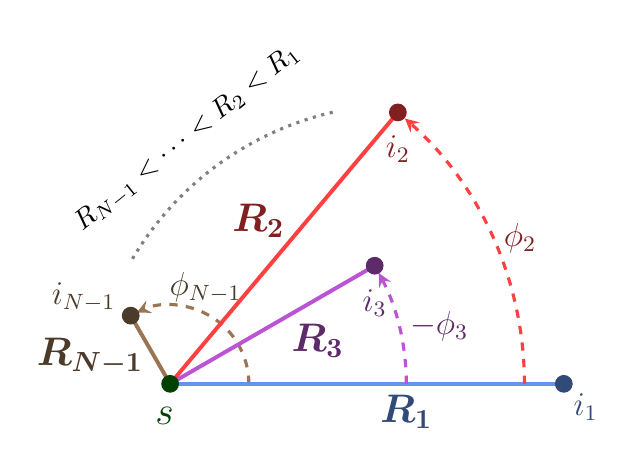
\begin{tikzpicture}
% Defining colors
\definecolor{cornflowerblue}{rgb}{0.39, 0.58, 0.93}
\definecolor{azure(colorwheel)}{rgb}{0.0, 0.5, 1.0}

\definecolor{coralred}{rgb}{1.0, 0.25, 0.25}
\definecolor{cadmiumorange}{rgb}{0.93, 0.53, 0.18}
\definecolor{darkgoldenrod}{rgb}{0.72, 0.53, 0.04}

\definecolor{rosevale}{rgb}{0.67, 0.31, 0.32}
\definecolor{palebrown}{rgb}{0.6, 0.46, 0.33}

\definecolor{mediumorchid}{rgb}{0.73, 0.33, 0.83}

\definecolor{ao}{rgb}{0.0, 0.5, 0.0}
\definecolor{lightseagreen}{rgb}{0.13, 0.7, 0.67}

% Defining colors associated with different nodes
\colorlet{colsp}{ao}
\colorlet{coli1}{cornflowerblue}
\colorlet{coli2}{coralred}
\colorlet{coli3}{mediumorchid}
\colorlet{coliN}{palebrown}

% All grey
% \colorlet{colsp}{gray}
% \colorlet{coli1}{gray}
% \colorlet{coli2}{gray}
% \colorlet{coli3}{gray}
% \colorlet{coliN}{gray}



% =:=:=:=:=:=:=:=:=:=:=:=:=:=:=:=:=:=:=
% Particle N
% =:=:=:=:=:=:=:=:=:=:=:=:=:=:=:=:=:=:=
% Beginning here so it is on the back layer
\draw[color=coliN, line width=0.5mm]
    (0, 0) -- (120:1.0) coordinate (iN)
    node[pos=0.4, left, text=black, font=\Large]
    {\textcolor{coliN!50!black}{$\boldsymbol{R_{N-1}}$}};

\newif\ifrecursive
\recursivefalse
\ifrecursive
% Sketch of N-1
\draw[color=gray, dashed, line width=0.5mm]
    (0, 0) -- (75:1.6) coordinate (iNm)
    node[pos=0.4, left, text=black, font=\Large] {};
% iN-1 node
\filldraw[color=gray]
    (iNm) circle (3pt)
    node[above, xshift=-5pt, yshift=2pt]
    {\textcolor{gray!60!black}{$i_{N-2}$}};
% phi_N arc
\draw[-stealth, color=coliN, dashed, line width=0.4mm]
    (75:1.0)
    arc[start angle=75, end angle=115, radius=1.0]
    node[pos=0.55, above, text=black, font=\large]
    {\textcolor{coliN!50!black}{$\phi_{N-1}$}};
\else
% phi_N arc
\draw[-stealth, color=coliN, dashed, line width=0.4mm]
    (0:1.0)
    arc[start angle=0, end angle=115, radius=1.0]
    node[pos=0.55, above, text=black, font=\large]
    {\textcolor{coliN!50!black}{$\phi_{N-1}$}};
\fi

% iN node
\filldraw[color=coliN!50!black]
    (iN) circle (3pt)
    node[above left, xshift=-2pt, yshift=-2pt, font=\large]
    {\textcolor{coliN!50!black}{$i_{N-1}$}};

% =:=:=:=:=:=:=:=:=:=:=:=:=:=:=:=:=:=:=
% Particle 1
% =:=:=:=:=:=:=:=:=:=:=:=:=:=:=:=:=:=:=
\draw[color=coli1, line width=0.5mm]
    (0, 0) -- (0:5) coordinate (i1)
    node[pos=0.6, below, sloped, text=black,
         font=\Large]
        {\textcolor{coli1!50!black}{$\boldsymbol{R_1}$}};

% i1 node
\filldraw[color=coli1!50!black]
    (i1) circle (3pt)
    node[below right, font=\large]
    {\textcolor{coli1!50!black}{$i_1$}};

% =:=:=:=:=:=:=:=:=:=:=:=:=:=:=:=:=:=:=
% Particle 2
% =:=:=:=:=:=:=:=:=:=:=:=:=:=:=:=:=:=:=
\draw[color=coli2, line width=0.5mm]
    (0, 0) -- (50:4.5) coordinate (i2)
    node[pos=0.6, left, text=black, xshift=-4pt, font=\Large]
    {\textcolor{coli2!50!black}{$\boldsymbol{R_2}$}};

% phi_2 arc
\draw[-stealth, color=coli2, dashed, line width=0.4mm]
    (0:4.5)
    arc [start angle=0, end angle=48.5, radius=4.5]
    node[pos=0.5, right, text=black, font=\large]
    {\textcolor{coli2!50!black}{$\phi_2$}};

% i2 node
\filldraw[coli2!50!black]
    (i2) circle (3pt)
    node[below, yshift=-5pt, font=\large]
    {\textcolor{coli2!50!black}{$i_2$}};


% =:=:=:=:=:=:=:=:=:=:=:=:=:=:=:=:=:=:=
% Particle 3
% =:=:=:=:=:=:=:=:=:=:=:=:=:=:=:=:=:=:=
\draw[color=coli3, line width=0.5mm]
    (0, 0) -- (30:3) coordinate (i3)
    node[pos=0.6, below, text=black, xshift=9pt, font=\Large]
    {\textcolor{coli3!50!black}{$\boldsymbol{R_3}$}};

\ifrecursive
% phi_3 arc
\draw[-stealth, color=coli3, dashed, line width=0.4mm]
    (50:3.0)
    arc [start angle=50, end angle=32, radius=3.0]
    node[pos=0.3, right, xshift=2pt, text=black, font=\large]
    {\textcolor{coli3!50!black}{$-\phi_3$}};
\else
% phi_3 arc
\draw[-stealth, color=coli3, dashed, line width=0.4mm]
    (0:3.0)
    arc [start angle=0, end angle=28, radius=3.0]
    node[pos=0.5, right, text=black, font=\large]
    {\textcolor{coli3!50!black}{$-\phi_3$}};
\fi

% i3 node
\filldraw[color=coli3!50!black]
    (i3) circle (3pt)
    node[below, yshift=-5pt, font=\large]
    {\textcolor{coli3!50!black}{$i_3$}};




% =:=:=:=:=:=:=:=:=:=:=:=:=:=:=:=:=:=:=
% Draw the central point s
% =:=:=:=:=:=:=:=:=:=:=:=:=:=:=:=:=:=:=
\filldraw[color=colsp!50!black]
    (0, 0) circle (3pt)
    node[below, yshift=-5pt, xshift=-2pt, font=\Large]
    {\textcolor{colsp!50!black}{$s$}};


% =:=:=:=:=:=:=:=:=:=:=:=:=:=:=:=:=:=:=
% Draw ellipses to indicate missing points
% =:=:=:=:=:=:=:=:=:=:=:=:=:=:=:=:=:=:=
\draw[gray, dotted, line width=0.4mm,
      xshift=-0.00cm, yshift=0.50cm]
      (55:3.6)
    arc[start angle=103, end angle=150, radius=4.]
    node[pos=0.55, sloped, above,
         xshift=0.1cm, yshift=0.2cm, text=black]
        {$R_{N-1} < \cdots < R_2 < R_1$};

\end{tikzpicture}

    }
    \caption[Cartoon of the new parameterization of ENCs introduced by the author and collaborators]{
        A cartoon of the new parametrization of ENCs we introduce in \Eqs{new_def}{renc}.
        %
        Instead of computing the ENC using all \(\binom{N}{2}\) pairwise distances, we parametrize the ENC with \(2N - 3\) oriented polar coordinates centered on a special particle \izero{}, and then perform a momentum-weighted sum over all choices for \izero{}.
    }
	\label{fig:cartoon}
\end{figure}


\begin{definitionbox}{New PENC Parametrization}{}
    Our new parametrization of \glspl{penc}, with a simpler phase space structure, takes the form:
    %%%
    \begin{align}
        \label{eq:new_def}
        \frac{\dd \Sigma_\text{PENC}}{\dd R_1}
        :=
        \frac{1}{\sigma}\frac{\dd \sigma_N}{\dd R_1}
        &=
        \biggl\langle
            \sum_{\izero=1}^M  z_{\izero} \!\!
            \sum_{i_1 \dots i_{N-1}}
           \!\! z_{i_1} \dots z_{i_{N-1}}
            \delta (
                R_1
                \!-\!
                \max_j\{R_{\izero,i_j}\}
            ) \!
        \biggr\rangle ,
        \notag \\
        &=: \text{PENC}(R_1) \,
        .
    \end{align}
    %%%
    %
    The sums on \(\izero\) and \(\{i_j\}_{j=1}^{N-1}\) again run over all $M$ particles within a jet.
    %
    The crucial simplification is that our \gls{penc} is based on a new variable, \(R_1\), that indicates the maximum distance \(\max\{R_{\izero, i_j}\}\) between the \textit{single} particle \(\izero\) and any of the remaining $N-1$ particles \(\{i_j\}_{j=1}^{N-1}\).
\end{definitionbox}


\begin{figure}
    \centering
    \includegraphics[width=0.8\textwidth]{figures/eec-angles/ENC.pdf}
    \caption[%
        Comparisons of the new and traditional parameterizations of projected ENCs.
        %
        Figure by Ankita Budhraja.
    ]{
        \gls{penc} distributions for $N \in \{3, 4.5, 6\}$, calculated using our new parametrization (solid) and the traditional parametrization (dashed).
        %
        $R_{*}$ denotes the largest distance to the special particle for our new parametrization ($R_1$), and the largest separation between the $N$ particles for the traditional one ($R_L$).
        %
        The differences are small in the perturbative region $R_{*} \!\! \gg  \! \Lambda_{\rm QCD} /p_T$, but become noticeable in the transition between perturbative and non-perturbative regimes (indicated by the vertical dashed lines).
        %
        Figure by Ankita Budhraja.
    }
	\label{fig:ENC}%
\end{figure}

\indent
Like the old variable \(R_L\) of \Eq{old_def}, \(R_1\) still roughly characterizes the maximum angular scale between a set of \(N\) particles, since \(R_L/2 \leq R_1 \leq R_L\) by the triangle inequality.
%
Indeed, the \glspl{penc} displayed in \Fig{ENC} show that the difference between our parametrization and that of \Eq{old_def} is small, and that both parametrizations have similar scaling behavior in the perturbative region (though there are some differences in the perturbative to non-perturbative transition).
%
\Figss{ENC}{bullseye}{density} all feature energy correlators evaluated on the CMS 2011A Jet Primary Dataset~\cite{CERNOpenDataPortal, CMS:JetPrimary2011A}, also available in MIT Open Data format~\cite{Komiske:2019jim, komiske_patrick_2019_3340205}, on jets with transverse momenta $p_{T}^{\text{jet}} \in [500, 550]$ GeV and pseudo-rapidity $\vert \eta^{\rm jet} \vert < 1.9$.

\indent
A major strength of the parameterization of \Eq{new_def} it its dramatically improved computational efficiency relative to older \gls{penc} paramterization.
%
The computational efficiency of our parametrization is more clear in the expression for (normalized) cumulative distribution:
%%%
\begin{align} \label{eq:new_cml}
  \Sigma_N(R_1)
  \!
  &=
  \!
  \frac{1}{\sigma}
  \int_0^{R_1}
  \!\!
  \dd R_1'
  \,
  \frac{\dd \sigma_N}{\dd R_1'}
   % \notag \\
  =
  % \!
  \biggl\langle \sum_{\izero} z_{\izero} [z_{\rm disk}(\izero,R_1)]^{N-1}
  \biggr\rangle
  ,
\end{align}
%%%
where $z_{\rm disk}(\izero,R_1)$ denotes the total transverse momentum fraction of all particles within a radius $R_1$ of the special particle \izero{}.
%
Notably, the simple form of \Eq{new_cml} holds even for non-integer $N$.
%
A practical way to evaluate \Eq{new_cml} (and \Eq{new_def} after differentiation) is, for each $\izero$, to first sort all particles by their distance with respect to $\izero$, and then to compute $\Sigma_N(R_1)$ by beginning with $R_1=0$ and then increasing it.
%
Sorting particles by their distance to \izero{} takes $M\ln M$ time, and the remaining sum over \izero{} scales with $M$, resulting in an overall computation time scaling as $M^2 \ln M$.
%
This computational speed up is especially interesting for heavy-ion collisions where $M$ is typically very large.


The factorization formula in \Eq{factorization_defn} can be extended to that of traditionally-parameterized \glspl{penc}~\cite{Chen:2020vvp}.
%
The factorization for existing \glspl{penc} also applies to our new parameterization, with one small difference:
%
because the variables $R_1$ and $R_L$ differ for three or more emissions, the jet function for our \glspl{penc} differs from the old one at $\ord{\alpha_s^2}$, or at next-to-next-to-leading logarithmic accuracy (NNLL).
%
In \Prob{nll_equiv}, we discuss how the NLL equivalence of jet functions implies that $
    \Sigma_N
    (R_L)
    =
    \Sigma_N(
    R_1 = R_L[
        1
        +
        \mathcal{O}
        (
        \alpha_s
        )
    ]
    )
$%
.
%
Furthermore, at NNLL and beyond, we expect that the simple dependence of \Eq{new_cml} on $N$ will substantially simplify the calculation of the jet function for $R_1$.
%
By contrast, the jet function using the old parametrization requires dedicated calculations for each individual value of $N$~\cite{Dixon:2019uzg,Chen:2023zlx}.




\remark{}{
    The cumulative distribution associated with our new \gls{penc} parametrization, given in \Eq{new_cml}, is the $N$-th Mellin moment in $z$ of
    %%%
    \begin{align}
        \frac{1}{\sigma}
        \frac{\dd \sigma}{\dd z}
        (R_1)
        =
        \Bigl
        \langle\sum_{\izero} z_{\izero}\, \delta
        \bigl[
            z
            -
            z_{\rm disk}(\izero,R_1)
        \bigr]
        \Bigr\rangle
        \,,
    \end{align}
    %%%
    which is also the differential jet rate in a ``jets-without-jets approach'' if \(R_1\) is treated as a jet radius~\cite{Bertolini:2013iqa,Bertolini:2015pka}.
    %
    A similar moment relation between the jet rate and the original ENC was noted in Ref.~\cite{Lee:2024icn}.
}





% ----------------------------------------------
\subsection{Resolved Energy Correlators}
% ----------------------------------------------
\label{sec:enc-resolved}

By including (or \emph{resolving}) more detailed angular information about the positions and relative orientations of particles within the jet, we may generalize our new parametrization for the \gls{penc} to introduce the \gls{renc}:


\begin{definitionbox}{Resolved Energy Correlator (RENC)}{renc}

    \vocab{\glslink{renc}{Resolved Energy Correlators (RENCs)}} are defined as the correlators

    \begin{align}
        \label{eq:renc}
        &\text{RENC}(R_1, R_2, \phi_2, R_3, \phi_3, \dots)
        := \frac{1}{\sigma}
        \frac{\dd \sigma_N}{\dd R_1 \dd R_2 \dd \phi_2 \dd R_3 \dd \phi_3 \dots} \notag
        \\
        &
        = \biggl\langle
        \sum_{\izero}
        z_{\izero}
        \!\!
        \sum_{i_1 \geq\dots\geq i_{N-1}}
        \!\!\!\!
        z_{i_1} \dots z_{i_{N-1}}
        \binom{N}{n_1\,n_2\, \dots}\,
        \delta
            (R_1 \!-\! R_{\izero,i_1}
        )
        \notag
        \\
        & \qquad\qquad\qquad\qquad
        \ \times
        \rho_{i_2}(R_2,\phi_2)\, \rho_{i_3}(R_3,\phi_3)\, \dots\biggr\rangle
        \, ,
    \end{align}
    %%%
    where for each $s$, the $i_j$ are indexed such that $R_{s,i_1} \ge R_{s,i_2} \ge \ldots$, and the summand involves the per-particle densities:
    %%%
    \begin{align}
        \rho_{i_j}(R_j, \phi_j)
        =
        \delta(
            R_j
            -
            R_{\izero,i_j}
        )\,
        \delta(
            \phi_j
            -
            \phi_{i_{j-1},i_j}
        )
    \,.\end{align}
    %%%
    The ``$\dots$" correspond to additional  \(R_j\) and \(\phi_j\), and $n_k$ denotes how often particle $k$ of the jet appears among the $i_j$ (such that terms with $n_k>1$ encode self-correlations of particle $k$), with $\sum^M_{k=1} n_k = N$.

\end{definitionbox}


\begin{figure}
    \centering
    \subfloat[]{
    	\includegraphics[width=0.33\textwidth]{figures/eec-angles/opendata/od_3particle_bullseye_0.286592.pdf}
        \label{fig:bullseye_new}
     }
     \subfloat[]{
    	\includegraphics[width=0.33\textwidth]{figures/eec-angles/opendata/od_3particle_old_bullseye_0.286592.pdf}
        \label{fig:bullseye_old}
     }
    \subfloat[]{
    	\includegraphics
        [width=0.33\textwidth]
        {figures/eec-angles/supplemental/3particle/w0.216087_3particle_bullseye.pdf}
        \label{fig:bullseye_new_w}
    }
    \caption[Polar heat maps of three-point energy correlators.]{
        Polar heat maps visualizing \textbf{(a)} our new RE3C applied to CMS Open Data, \textbf{(b)} the traditional E3C applied to CMS Open Data, and \textbf{(c)} our new parametrization applied to $W$-boson-initiated jets from \texttt{Pythia 8.310}.
        %
        In \textbf{(a)} and \textbf{(c)}, the radial variables correspond to \(R_2/R_1\), the polar angle corresponds to \(\phi_2\), and we show the RE3C in the bin $R_1 \in [0.27,0.3]$.
        %
        In \textbf{(b)} the radius corresponds to \(R_S/R_L\), the polar angle corresponds to the angle between associated lines of length \(R_S\) and \(R_L\), and we show the E3C in the bin $R_L \in [0.27,0.3]$.
        %
        In all three plots, we see collinear enhancements for the RE3C near the origin, when two particles become very close in angle.
        %
        In \textbf{(a)} and \textbf{(c)}, we also see collinear enhancements as \(R_2/R_1 \to 1\) and \(\phi_2 \to 0\), and \textbf{(c)} exhibits additional non-collinear enhancements correlated with the \(W\)-boson mass.
    }
	\label{fig:bullseye}%
\end{figure}



\begin{figure}
\centering
    \subfloat[]{
        \includegraphics
        [width=0.33\textwidth]{figures/eec-angles/od_newdef_density.pdf}
    	\label{fig:density_new}%
    }
    \subfloat[]{
        \includegraphics
        [width=0.33\textwidth]
        {figures/eec-angles/od_olddef_density.pdf}
    	\label{fig:density_old}%
    }
    \subfloat[]{
        \includegraphics
        [width=0.33\textwidth]
        {figures/eec-angles/supplemental/density/w_newdef_density.pdf}
    	\label{fig:density_w}%
    }
    \caption[Three-point energy correlators integrated over azimuthal angle.]{
        Normalized distributions \textbf{(a)} our new RE3C applied to CMS Open Data when integrated over the azimuthal angle \(\phi_2\), \textbf{(b)} the traditional E3C applied to CMS Open Data integrated over the intermediate angle $R_M$ (analogous to integrating over \(\phi_s\)), and \textbf{(c)} our new, \(\phi_2\)-integrated RE3C applied to $W$-boson-initiated jets.
    }
	\label{fig:density}%
\end{figure}





Our parametrization is visualized in \Fig{cartoon}, and utilizes polar coordinates around $\izero$, ordered in radius $R_1 \! > \! R_2 \! > \! \dots$ and with an \emph{oriented} azimuthal angle $\phi_j$ taken relative to the $(j\!-\!1)$-th resolved emission.
%
The \(R_j\) and \(\phi_j\) use \(2N-3\) variables to completely characterize the positions of all particles in the jet, relative to the axis defined by particles \(s\) and \(i_1\).
%
The multinomial coefficient in \Eq{renc} arises due to the ordering of the \(R_j\), and accounts for the possibility that two or more of the $i_j$ may be equal.
%
Integrating inclusively over $\{R_j, \phi_j\}_{j=2}^{N}$ (which sets the third line of \Eq{renc} to unity) reduces the \gls{renc} to the \gls{penc} from \Eq{new_def}.


The \glspl{renc} we introduce also preserve information about relative orientations, whereas even in the simple example of $N=3$, the traditional E3C parametrization in terms of the largest ($R_L$), medium ($R_M$), and shortest ($R_S$) distances does not.
%
We visualize the additional orientation information preserved by our RE3Cs in \Figs{bullseye_new}{bullseye_old}, where we compare polar heat maps of our parametrization of the RE3C to the traditional paramterization of the E3C.
%
The additional angular information carried by our new RE3C also leads to striking visual differences when comparing jets initiated by different processes.
%
For example, the unique characteristics of the RE3C evaluated on $W$-boson initiated jets generated with \texttt{Pythia 8.310}, shown in \Fig{bullseye_new_w}, clearly distinguish it from the RE3C of QCD-initiated jets.
%
This qualitative difference is not visible in the traditional parametrization, as shown in the supplemental material together with similar visualizations for additional processes.


We also note that each additional resolved particle (i.e.\ each \((R_j, \phi_j)\) pair) introduces a factor of $M$ to the scaling of the \gls{renc} computation time.
%
In contrast, the computation time for e.g.~the traditional 4-point correlator scales as $M^4$ independent of how many angles were resolved.


In \Fig{runtime}, we display the computational runtime of our code for the evaluation of \glspl{penc} and \glspl{renc} on jet samples from CMS Open Data.
%
\Fig{runtime_scaling} shows how the scaling time for each nearly follows an \(M^r\) scaling, where \(r\) indicates the number of resolved emissions.
%
Furthermore, the independence of the runtime on the value of \(N\) allows us to compute the \gls{penc} for enormous, and previously unimaginable, values of \(N\);
%
some examples up to \(N = 100\) are shown in \Fig{runtime_largeN}.
%
We highlight that our implementation takes similar runtime for all values of $N$.
%
Therefore, we expect the \gls{penc} we introduce in this work to significantly benefit ongoing studies which apply energy correlators in jets produced in heavy-ion collisions for revealing the emergent scales of the quark-gluon plasma in these environments.

\begin{figure}[t!]
    % \centering
    \subfloat[]{
        \includegraphics[width=.45\textwidth]{figures/eec-angles/opendata/opendata_runtimes_fewM.pdf}
        \label{fig:runtime_scaling}
    }
    $\qquad$
    \subfloat[]{
        \includegraphics[width=.45\textwidth]{figures/eec-angles/opendata/od_projected_runtime.pdf}
        \label{fig:runtime_largeN}
    }
    \caption[Plots emphasizing the computational performance of the new parameterization of energy correlators discussed in this work.]
    {
        Plots emphasizing the computational performance of the energy correlators we introduce in this work.
        %
        \sam{fix, together wtih the other ref comments}
        %
        \textbf{(a)}
        Runtime of the \gls{penc} and \gls{renc} code of Ref.~\cite{github:RENC} on CMS Open Data as a function of the number of particles in a jet, together with a polynomial fit to guide the eye.
        %
        \textbf{(b)}
        \glspl{penc} for $N=$ 2, 5, 10, 50, and 100, each computed using on \(10^5\) CMS Open Data jets in less than thirty seconds.
        %
        The solid lines show the \glspl{penc} introduced in this work, and the dashed lines show the traditional \glspl{penc}.
        %
        Even for $N=5$, the traditional computation takes $6266$ seconds (close to 2 hours) to run on the same CMS Open Data samples, and the computation time grows exponentially as $N$ increases.
        %
        The large values of $N$, which are computationally inaccessible to the traditional \gls{penc} even for $N=10$, are chosen to stress that the \glspl{penc} we introduce in this work make quick work of previously unimaginable computations.
    }
	\label{fig:runtime}%
\end{figure}




\remark{}{
    The squeezed limit of our new RE3C, \(R_2 \ll R_1\), is quite similar to the squeezed limit of the traditional E3C, \(R_S \ll R_L\);
    %
    in this limit, \(R_2 \!\! \sim \!\! R_S\) and \(R_1 \!\! \sim \!\! R_L\).
    %
    Our new RE3C and the traditional E3C evaluated on CMS Open Data are compared in \Figs{density_new}{density_old}, which demonstrate that they indeed take similar forms when \(R_S / R_L,\,R_2/R_1 < \! \frac{1}{2}\).
    %
    When $R_S/R_L \!\! > \!\! \frac{1}{2}$, however, the traditional E3C is suppressed due to the hierarchy $R_S < R_M < R_L$.
    %
    In \Fig{density_w}, we visualize our new RE3C on \texttt{Pythia}-generated \(W\) jets, which exhibits a non-perturbative ridge similar to the one seen in CMS Open Data as well as additional features at \(R_1 = 0.3\) correlated with the \(W\) mass, \(R_1 \sim 2 m_W / p_T\).
    %
    In \Prob{enc-nonpert}, we explain the ridge-like features in these plots from the perspective of non-perturbative physics.
}


For completeness, we also mention two additional generalizations of our new parametrization for energy correlators -- \glspl{renc} with two special particles and \glspl{renc} with two projected angles -- for which we defer more detailed explorations to future work.
%
For the energy correlator with two special particles,
%%%
\begin{align}
    \label{eq:two_special}
    &\frac{1}{\sigma} \frac{\dd \sigma_{N,N'}}
    {\dd R\, \dd R_1\, \dd R_1'}
    =
    \biggl\langle
    \sum_{\izero}
    z_{\izero}  \sum_{\izero'}
    z_{\izero'}\,
    \delta(R - R_{\izero\izero'})
    \\
    & \quad \times
    \sum_{i_1 \dots i_{N-1}}
    z_{i_1} \dots z_{i_{N-1}}
    \delta (R_1 - \max\{R_{\izero,i_k}\})
    \notag
    \\
    &
    \quad  \times
    \sum_{j_1 \dots j_{N'-1}}
    z_{j_1} \dots z_{j_{N'-1}}
    \delta (R_1' - \max\{R_{\izero',j_k}\})
    \biggr
    \rangle
    \notag\,,
 \end{align}
%%%
the two special particles $\izero$ and $\izero'$ are separated by a distance $R$, and $R_1$ and $R_1'$ denote the maximum distance of other particles to $\izero$ and $\izero'$, respectively.
%
This parametrization may capture interesting features of the radiation patterns of intrinsically 2-prong jets, e.g.~from the hadronic decays of $W$ or Higgs bosons, with a straightforward extension to three or more special particles for higher-prong jets.


We also define a \emph{double}-projected energy-correlator,
%%%
\begin{align}
    \label{eq:double_projected}
    \frac{1}{\sigma}
    \frac{\dd \sigma_{(a, b)}}{\dd R_1\, \dd R_2}
    &=
    \biggl\langle \sum_{\izero} z_{\izero}
    \sum_{i_1 \dots i_{a}}
    z_{i_1} \dots z_{i_{a}}
    \delta(R_1 \!-\! \max\{R_{\izero,i_k}\})
    \notag
    \\
    & \times
    \sum_{j_1 \dots j_{b}}
    z_{j_1} \dots z_{j_{b}}
    \delta (R_2 - \max\{R_{\izero,j_k}\}) \biggr\rangle
    \,,
\end{align}
%%%
where we again take $R_1>R_2$.
%
The associated cumulative distribution, analogous to \Eq{new_cml}, is
%%%
\begin{align}
    \label{eq:double_projected_cml}
    &
    \Sigma_{(a,b)}(R_1,R_2)
    =
    \frac{1}{\sigma}
    \int_0^{R_1}
    \!
    \dd R_1'   \int_0^{R_2}
    \!
    \dd R_2'
    \,
    \frac{\dd \sigma_{a,b}}{\dd R_1'\, \dd R_2'}
    \notag
    \\
    & \quad
    =
    \Bigl\langle \sum_{\izero}
    z_{\izero}
    [z_{\rm disk}(\izero,R_1)]^a [z_{\rm disk}(\izero,R_2)]^b \Bigr\rangle
    \,,
\end{align}
%%%
highlighting that there is no additional complication when $a,b$ are non-integer.
%
Because the effective scaling of this observable is set by $N = 1+a+b$ and because the $N= 1$ moment of the DGLAP splitting functions vanish, we expect very mild dependence on $R_1$ at fixed $R_2/R_1$ when $b = -a$.
%
This behavior therefore offers an interesting test of parton shower generators.



% ----------------------------------------------
\subsection{Process Dependence of Higher-Point Correlators}
% ----------------------------------------------
\label{sec:enc-pheno}

In this section, we survey the behavior of our new parameterization for energy correlators on a variety of jet samples.
%
We first provide additional polar heat maps, or \textit{bullseye} visualizations, of RE3Cs and RE4Cs evaluated on CMS Open Data, which yield an intuitive view into the internal structure of jets enabled by our new parametrization.
%
Then, we visualize for energy correlators evaluated on Monte Carlo samples of QCD-, \(W\)-, and top-initiated jets generated in \texttt{Pythia 8.310}, as detailed in Table~\ref{tab:samples}, which emphasize both the broad range of applications and the visually intuitive representations of jet substructure that are achieved by our new parametrization for RE3Cs.
%
We expect that similar visualizations will benefit current and future studies of jet substructure at the LHC.


The bullseyes for the RE3C evaluated on CMS Open Data, shown in \Fig{cms_re3cs}, have a radial variable corresponding to the ratio \(R_2/R_1 < 1\), with a polar angle corresponding to \(\phi_2\).
%
Similarly, the bullseyes for the RE4C evaluated on CMS Open Data, in \Fig{cms_re4cs}, use the radial variable \(R_3/R_2 < 1\) and the corresponding polar variable \(\phi_3\).
%
The bullseyes are normalized to a radial measure, such that the bullseye plots provide a faithful representation of each correlator;
%
for the RE3C, the bullseye is normalized to unity against the measure \(\dd\log R_1 \times R_2 \dd R_2 \dd \phi_2\), while the bullseyes for the RE4C are normalized to unity against \(\dd \log R_1 \dd (R_2/R_1) \dd \phi_2  \times R_3 \dd R_3 \dd \phi_3\)

RE3Cs are shown in \Fig{cms_re3cs} for several \(R_1\) bins, and RE4Cs are shown in \Fig{cms_re4cs} for several \(R_1\) and \(\phi_2\) bins with a fixed \(R_2/R_1\) bin.
%
We note that the RE3C distributions are quite similar across different \(R_1\) bins.
%
On the other hand, for \(R_2\) near \(R_1\), the RE4C distributions exhibit distinct patterns of radiation depending on the value of \(\phi_2\).
%
In particular, \Fig{cms_re4cs} prominently visualizes the collinearly enhanced correlations in the RE4C when \(\phi_3\) is near \(-\phi_2\) and \(R_3\) is near \(R_1\), i.e.~when particle \(i_3\) approaches particle \(i_1\).
%
For small \(R_2\), these correlations diminish, and the bullseye visualizations for the RE4C look very similar to that of the RE3C, reflecting the near-scale-invariance of QCD.

\vspace{20pt}

\begin{figure}[ht!]
    \vspace{-20pt}
    \centering
    \subfloat[]{
    	\includegraphics[width=0.32\textwidth]{figures/eec-angles/opendata/od_3particle_bullseye_0.0299352.pdf}
     }
    \subfloat[]{
    	\includegraphics[width=0.32\textwidth]{figures/eec-angles/opendata/od_3particle_bullseye_0.101766.pdf}
     }
    \subfloat[]{
    	\includegraphics[width=0.32\textwidth]{figures/eec-angles/opendata/od_3particle_bullseye_0.286592.pdf}
     }
     \caption[Additional polar heat maps for RE3Cs evaluated on CMS Open Data.]
    {
        Additional polar heat maps for RE3Cs evaluated on CMS Open Data.
        %
        There are enhanced correlations when \(R_2\sim 0\), corresponding to the collinear enhancement
        as \(i_2\) approaches \(s\), and when \(\phi_2 \sim 0\), \(R_2 \sim R_1\), corresponding to \(i_2 \to\) \(i_1\).
        %
        The \(R_1\) bin for each plot is indicated by the radius of the filled circle in the top-left inset of each plot.
    }
    \label{fig:cms_re3cs}
\end{figure}
\begin{figure}[ht!]
    % \centering
    \subfloat[]{
    	\includegraphics[width=0.32\textwidth]{figures/eec-angles/opendata/od_4particle_bullseye_0.0401108_0.82_0.753982.pdf}
    }
    \subfloat[]{
    	\includegraphics[width=0.32\textwidth]{figures/eec-angles/opendata/od_4particle_bullseye_0.134694_0.82_0.753982.pdf}
    }
    \subfloat[]{
    	\includegraphics[width=0.32\textwidth]{figures/eec-angles/opendata/od_4particle_bullseye_0.246826_0.82_0.753982.pdf}
     }
    \\
    \vspace{-8pt}
     \subfloat[]{
    	\includegraphics[width=0.32\textwidth]{figures/eec-angles/opendata/od_4particle_bullseye_0.0401108_0.82_1.50796.pdf}
    }
    \subfloat[]{
    	\includegraphics[width=0.32\textwidth]{figures/eec-angles/opendata/od_4particle_bullseye_0.134694_0.82_1.50796.pdf}
    }
    \subfloat[]{
    	\includegraphics[width=0.32\textwidth]{figures/eec-angles/opendata/od_4particle_bullseye_0.246826_0.82_1.50796.pdf}
    }
    \\
    \vspace{-8pt}
     \subfloat[]{
    	\includegraphics[width=0.32\textwidth]{figures/eec-angles/opendata/od_4particle_bullseye_0.0401108_0.82_3.01593.pdf}
    }
    \subfloat[]{
    	\includegraphics[width=0.32\textwidth]{figures/eec-angles/opendata/od_4particle_bullseye_0.134694_0.82_3.01593.pdf}
    }
    \subfloat[]{
    	\includegraphics[width=0.32\textwidth]{figures/eec-angles/opendata/od_4particle_bullseye_0.246826_0.82_3.01593.pdf}
    }
    \caption[Polar heat maps for RE4Cs evaluated on CMS Open Data.]{
        Polar heat maps for RE4Cs evaluated on CMS Open Data, with \(\phi_2\) centered near $45^\circ$ (top row), $90^\circ$ (middle row) and $180^\circ$ (bottom row).
        %
        We highlight that, relative to the RE3C presented in \Fig{cms_re3cs}, there are enhanced correlations when \(\phi_3 \sim -\phi_2\), corresponding to the collinear enhancement of radiation as \(i_3\) approaches \(i_1\).
    }
    \label{fig:cms_re4cs}
\end{figure}



We now turn to our simulated samples of QCD, \(W\), and top jets.
%
We begin by showing \glspl{penc} evaluated on each jet sample in \Fig{pythia_pencs}, which provide simple, albeit less fetching, visualizations which clearly distinguish each sample of jets.
\begin{figure}[t]
    % \centering
    \subfloat[]{
    	\includegraphics[width=0.34\textwidth]{figures/eec-angles/supplemental/2particle/qcd_combined_1d.pdf}
    }
    \subfloat[]{
    	\includegraphics[width=0.34\textwidth]{figures/eec-angles/supplemental/2particle/w_combined_1d.pdf}
    }
    \subfloat[]{
    	\includegraphics[width=0.34\textwidth]{figures/eec-angles/supplemental/2particle/top_combined_1d.pdf}
    }
    \caption[Projected energy correlators on simulated QCD, \(W\), and top jets.]{
        \glspl{penc} for {\textbf{(a)}} QCD-, {\textbf{(b)}} $W$- and {\textbf{(c)}} top-quark-initiated jet samples generated with \texttt{Pythia 8.310}.
        %
        Jets are clustered using the anti-$k_t$ algorithm with a radius parameter of $R=0.8$, and have transverse momenta in the range $p_T^{\rm jet} \in [500,550] \,\text{GeV}$ and psuedo-rapidities in the range $\vert \eta^{\rm jet}\vert < 1.9$.
        %
        \glspl{penc} for $W$- and top-quark-initiated jets feature enhanced correlations at scales correlated with the $W$-boson and top-quark masses.
    }
	\label{fig:pythia_pencs}%
\end{figure}

The visually distinct features of each jet sample are even more evident as more particles are resolved, i.e.~by the RE3C and RE4C.
%
In \Fig{pythia_re3cs}, we present bullseye visualizations of the RE3C for each jet sample in several \(R_1\) bins;
%
as in the plots using CMS Open Data in the previous appendix, the radial variable and polar angle for each RE3C bullseye are the ratio \(R_2/R_1\) and the angle \(\phi_2\), respectively.
%
We note that the rings in the polar heat maps for the RE3C are correlated with the mass of the \(W\) boson, in that they appear at the angular scale \(R_2 \simeq 0.3 \sim 2 m_W / p_T^\text{jet}\).

The bullseye of representation of the RE3C we introduce are similar to the analogous bullseye representations of the traditional E3C for each jet sample, shown in \Fig{pythia_old_e3cs}, for which the radial variable is the ratio \(R_S/R_L\) and the polar angle is the associated azimuthal angle.
%
However, the traditional E3C shows only a small slice of the information of the RE3C we introduce in this work, and the RE3C introduced in this work contains additional information about the relative orientations of particles within a jet;
%
for example, \Figs{w_medium_re3c}{w_large_re3c} can be compared to \Figs{w_medium_trade3c}{w_large_trade3c} to conclude that the RE3C we introduce conveys additional information about the orientation of the rings of radiation within \(W\)-boson-initiated jets.

\begin{figure}
    \centering
    \subfloat[]{
    	\includegraphics[width=0.34\textwidth]{figures/eec-angles/supplemental/3particle/qcd0.0225708_3particle_bullseye.pdf}
    }
    \subfloat[]{
    	\includegraphics[width=0.34\textwidth]{figures/eec-angles/supplemental/3particle/w0.0225708_3particle_bullseye.pdf}
    }
    \subfloat[]{
    	\includegraphics[width=0.34\textwidth]{figures/eec-angles/supplemental/3particle/top0.0225708_3particle_bullseye.pdf}
    }
    \\
    \subfloat[]{
    	\includegraphics[width=0.34\textwidth]{figures/eec-angles/supplemental/3particle/qcd0.0698374_3particle_bullseye.pdf}
    }
    \subfloat[]{
    	\includegraphics[width=0.34\textwidth]{figures/eec-angles/supplemental/3particle/w0.0698374_3particle_bullseye.pdf}
    }
    \subfloat[]{
    	\includegraphics[width=0.34\textwidth]{figures/eec-angles/supplemental/3particle/top0.0698374_3particle_bullseye.pdf}
    }
    \\
    \subfloat[]{
    	\includegraphics[width=0.34\textwidth]{figures/eec-angles/supplemental/3particle/qcd0.216087_3particle_bullseye.pdf}
    }
    \subfloat[]{
    	\includegraphics[width=0.34\textwidth]{figures/eec-angles/supplemental/3particle/w0.216087_3particle_bullseye.pdf}
        \label{fig:w_medium_re3c}
    }
    \subfloat[]{
    	\includegraphics[width=0.34\textwidth]{figures/eec-angles/supplemental/3particle/top0.216087_3particle_bullseye.pdf}
    }
    \\
    \subfloat[]{
    	\includegraphics[width=0.34\textwidth]{figures/eec-angles/supplemental/3particle/qcd0.668604_3particle_bullseye.pdf}
    }
    \subfloat[]{
    	\includegraphics[width=0.34\textwidth]{figures/eec-angles/supplemental/3particle/w0.668604_3particle_bullseye.pdf}
        \label{fig:w_large_re3c}
    }
    \subfloat[]{
    	\includegraphics[width=0.34\textwidth]{figures/eec-angles/supplemental/3particle/top0.668604_3particle_bullseye.pdf}
    }
    \caption[Polar heat maps of the resolved three-point energy corrleator on QCD, \(W\), and top jets.]{
        Polar heat maps of the RE3C we introduce in this work for (first column) QCD-, (second column) \(W\)-, and (third column) top-quark-initiated jets.
        %
        The radial direction in each plot is the ratio \(R_1/R_2\), and the polar angle of each plot indicates the angle \(\phi_2\).
        %
        Our RE3Cs provide a clear visual representation of the distinct patterns of radiation in each jet sample at different scales (set by \(R_1\)).
    }
	\label{fig:pythia_re3cs}%
\end{figure}

\begin{figure}
    \centering
    \subfloat[]{
    	\includegraphics[width=0.34\textwidth]{figures/eec-angles/supplemental/wedge/qcd0.0225708_3particle_bullseye.pdf}
    }
    \subfloat[]{
    	\includegraphics[width=0.34\textwidth]{figures/eec-angles/supplemental/wedge/w0.0225708_3particle_bullseye.pdf}
    }
    \subfloat[]{
    	\includegraphics[width=0.34\textwidth]{figures/eec-angles/supplemental/wedge/top0.0225708_3particle_bullseye.pdf}
    }
    \\
    \subfloat[]{
    	\includegraphics[width=0.34\textwidth]{figures/eec-angles/supplemental/wedge/qcd0.0698374_3particle_bullseye.pdf}
    }
    \subfloat[]{
    	\includegraphics[width=0.34\textwidth]{figures/eec-angles/supplemental/wedge/w0.0698374_3particle_bullseye.pdf}
    }
    \subfloat[]{
    	\includegraphics[width=0.34\textwidth]{figures/eec-angles/supplemental/wedge/top0.0698374_3particle_bullseye.pdf}
    }
    \\
    \subfloat[]{
    	\includegraphics[width=0.34\textwidth]{figures/eec-angles/supplemental/wedge/qcd0.216087_3particle_bullseye.pdf}
    }
    \subfloat[]{
    	\includegraphics[width=0.34\textwidth]{figures/eec-angles/supplemental/wedge/w0.216087_3particle_bullseye.pdf}
        \label{fig:w_medium_trade3c}
    }
    \subfloat[]{
    	\includegraphics[width=0.34\textwidth]{figures/eec-angles/supplemental/wedge/top0.216087_3particle_bullseye.pdf}
    }
    \\
    \subfloat[]{
    	\includegraphics[width=0.34\textwidth]{figures/eec-angles/supplemental/wedge/qcd0.668604_3particle_bullseye.pdf}
    }
    \subfloat[]{
    	\includegraphics[width=0.34\textwidth]{figures/eec-angles/supplemental/wedge/w0.668604_3particle_bullseye.pdf}
        \label{fig:w_large_trade3c}
    }
    \subfloat[]{
    	\includegraphics[width=0.34\textwidth]{figures/eec-angles/supplemental/wedge/top0.668604_3particle_bullseye.pdf}
    }
    \caption[Polar heat maps of the traditional three-point energy correlator on QCD, \(W\), and top jets.]{
        Polar heat maps of the traditional E3C for (first column) QCD-, (second column) \(W\)-, and (third column) top-quark-initiated jets.
        %
        The radial direction in each plot is the ratio \(R_S/R_L\), and the polar angle of the plot corresponds to the angle between the lines whose lengths determine \(R_S\) and \(R_L\).
        %
        The \(R_L\) bins for each plot are chosen to be the same as the \(R_1\) bins in \Fig{pythia_re3cs}.
        %
        The polar heat maps of the traditional E3C contain similar information as the RE3Cs introduced in this work and shown in \Fig{pythia_re3cs};
        %
        however, the traditional E3C does not capture all the orientation information about radiation patterns in each jet sample that is present in our new RE3C.
    }
	\label{fig:pythia_old_e3cs}%
\end{figure}

\Fig{pythia_re4cs} provides similar polar heat maps for \(R_3/R_2\) and \(\phi_3\) for the RE4C, within several \(\phi_2\) bins, and for \(R_2\) near \(R_1\).
%
As in the case of the RE4Cs evaluated on CMS Open Data, we also see prominent correlations when \(\phi_3 \sim -\phi_2\) when \(R_2\) is near \(R_1\), corresponding to the case that particle \(i_3\) approaches particle \(i_1\).
%
These correlations for \(\phi_3 \sim -\phi_2\) quickly diminish as \(R_2\) is decreased and no longer near \(R_1\).

\begin{figure}[t]
    \centering
    \subfloat[]{
    	\includegraphics[width=0.34\textwidth]{figures/eec-angles/supplemental/4particle/qcd0.452309_0.82_0.753982_4particle_bullseye.pdf}
    }
    \subfloat[]{
    	\includegraphics[width=0.34\textwidth]{figures/eec-angles/supplemental/4particle/w0.452309_0.82_0.753982_4particle_bullseye.pdf}
    }
    \subfloat[]{
    	\includegraphics[width=0.34\textwidth]{figures/eec-angles/supplemental/4particle/top0.452309_0.82_0.753982_4particle_bullseye.pdf}
    }
    \\
    \vspace{-8pt}
    \subfloat[]{
    	\includegraphics[width=0.34\textwidth]{figures/eec-angles/supplemental/4particle/qcd0.452309_0.82_1.50796_4particle_bullseye.pdf}
    }
    \subfloat[]{
    	\includegraphics[width=0.34\textwidth]{figures/eec-angles/supplemental/4particle/w0.452309_0.82_1.50796_4particle_bullseye.pdf}
    }
    \subfloat[]{
    	\includegraphics[width=0.34\textwidth]{figures/eec-angles/supplemental/4particle/top0.452309_0.82_1.50796_4particle_bullseye.pdf}
    }
    \\
    \vspace{-8pt}
    \subfloat[]{
    	\includegraphics[width=0.34\textwidth]{figures/eec-angles/supplemental/4particle/qcd0.452309_0.82_3.01593_4particle_bullseye.pdf}
    }
    \subfloat[]{
    	\includegraphics[width=0.34\textwidth]{figures/eec-angles/supplemental/4particle/w0.452309_0.82_3.01593_4particle_bullseye.pdf}
    }
    \subfloat[]{
    	\includegraphics[width=0.34\textwidth]{figures/eec-angles/supplemental/4particle/top0.452309_0.82_3.01593_4particle_bullseye.pdf}
    }
    \caption[Bullseye visualizations of the resolved four-point energy correlator.]{
        Bullseye visualizations of the RE4C evaluated on QCD-, \(W\)-, and top-quark-initiated jets generated with \texttt{Pythia 8.310}, in the style of \Fig{cms_re4cs}.
        %
        As in \Fig{cms_re4cs}, there are also enhanced correlations in energy when \(\phi_3\) is near \(-\phi_2\).
    }
	\label{fig:pythia_re4cs}%
\end{figure}

Finally, we visualize the \(\phi_2\)-integrated RE3Cs for each jet sample in the first row of \Fig{pythia_densities} and the \(R_M\)-integrated traditional E3Cs in the second row.
%
Much as in the case of the polar heat maps, the integrated RE3Cs densities provide strictly more information than the densities associated with traditional E3Cs. These provide a clear visual distinction between each sample of jets.

\begin{figure}[ht!]
    \centering
    \subfloat[]{
    	\includegraphics[width=0.34\textwidth]{figures/eec-angles/supplemental/density/qcd_newdef_density.pdf}
    }
    \subfloat[]{
    	\includegraphics[width=0.34\textwidth]{figures/eec-angles/supplemental/density/w_newdef_density.pdf}
    }
    \subfloat[]{
    	\includegraphics[width=0.34\textwidth]{figures/eec-angles/supplemental/density/top_newdef_density.pdf}
    }
    \\
     \subfloat[]{
    	\includegraphics[width=0.34\textwidth]{figures/eec-angles/supplemental/density/qcd_olddef_density.pdf}
    }
    \subfloat[]{
    	\includegraphics[width=0.34\textwidth]{figures/eec-angles/supplemental/density/w_olddef_density.pdf}
    }
    \subfloat[]{
    	\includegraphics[width=0.34\textwidth]{figures/eec-angles/supplemental/density/top_olddef_density.pdf}
    }
    \caption[Density plots of azimuthally-integrated resolved three-point energy correlators in QCD, \(W\), and top jets.]{
        Density plots for \(\phi_2\)-integrated RE3Cs (first row) and the analogous \(R_M\)-integrated traditional E3Cs (second row), in the style of Fig.~4 of the main text, evaluated on simulated events in \texttt{Pythia 8.310}.
        %
        The first column shows \(\phi_2\)-integrated RE3Cs for \(p p \to \) hadrons, the second column for \(p p \to W^+ W^-\), and the third column for \(p p \to t \bar t\).
        %
        Each row illuminates how three-point energy correlators encode the unique features of each type of jet.
        %
        We note that the information of the traditional E3C is a subset of the information conveyed by the RE3C we introduce in this work.
        %, and that our RE3C contains strictly more information about the three-particle correlations within each jet sample.
    }
	\label{fig:pythia_densities}%
\end{figure}




% ==============================================
\section{Energy-Weighted Observable Correlations (EWOCs)}
% ==============================================
\label{sec:ewocs}

Energy correlators are powerful tools for exploring the theory and phenomenology of particle collisions.
%
Rather than using grooming directly to modify the constituents of a jet to isolate partonic degrees of freedom, they use energy weighting to highlight correlations between the high-energy structures within a jet.
%
However, the EEC is limited to probing angular correlations, and angular correlations are not the only correlations of interest in particle collisions.
%
Additional, non-trivial steps are needed when using energy correlators to extract non-angular parameters of interest.

For example, we would like to emulate the discussion of \Sec{pira-mass} with energy correlators, and to use energy correlators rather than groomed jet masses to extract the top quark mass from particle collision data.
%
In this important example for modern particle physics analyses, the conversion of angular scales to mass scales involves the transverse momentum of top quark jets;
%
large experimental uncertainties in the jet \(p_T\) then directly affect the resulting extraction of the top quark mass \(m_t\).%
\footnote{
    A solution to this \(p_T\) smearing was proposed by the authors of \Reff{Holguin:2023bjf}, leveraging the \(W\)-bosons that emerge during top quark decay and the well-measured mass of the \(W\)-boson.
    %
    In particular, they define an integrated three-point energy correlator with two peaks, at angular scales \(\zeta_\text{peak} \sim m^2 / p_T^2\) with $m=m_W$ and $m=m_t$.
    %
    The ratio of the peak locations provides a robust measure of \(m_t/m_W\) which is insensitive to uncertainties in jet \(p_T\).
    %
    The approach we develop here does not rely on an existing, precisely determined particle mass.
}
%
Similarly, heavy-ion collisions and the properties of the QGP are characterized by a wide variety of correlations extending beyond the simple angular correlations probed by energy correlators \cite{Lokhtin:2004tx,Lokhtin:2006dp,Andres:2022ovj,Barata:2023zqg,Andres:2023xwr,Yang:2023dwc,Barata:2023vnl,Barata:2023bhh,Barata:2024nqo}.

% ---------------------------------------
\subsection{Introducing EWOCs}
% ---------------------------------------
\label{sec:ewoc-intro}



The framework of (subjet-level) \glslink{ewoc}{energy-weighted observable correlations (EWOCs)} that we expound in this section takes the mitigation of low-energy effects one step further.
%
In addition to using the energy weighting of the EEC, we use subjets instead of particles, and the subjet radius provides an explicit collinear cutoff on contributing radiation.%
\footnote{
    Subjet algorithms are not the only regularization schemes which provide a collinear cutoff on the physics of the EEC.
    %
    For example, \Reffs{Barata:2023bhh}{Budhraja:2024xiq} both compute the EEC on collinear-safe collective degrees of freedom based on the Lund plane or on the clustering history of the jet under study, respectively.
}
%
Any collection of particles which lead to the same subjet configurations will have the same EWOCs, regardless of the details of the particles themselves.

EWOCs therefore trade the ability to capture correlations between all particles in a jet for the ability to more easily control the effects of low-energy QCD.
%
As we will see, this tradeoff dramatically increases the richness of the correlations that can be probed by EWOCs.
As we discuss further in \Sec{ewoc-irc}, EWOCs are not collinear safe without an infra-red regulator;
%
therefore, we consider EWOCs which capture correlations between \textit{subjets}.%
\footnote{
    In principle, we could use any infra-red regulator.
    %
    \sam{steal}
}
%
These subjet EWOCs, which we will henceforth simply call EWOCs, have some important similarities and differences from the energy correlators defined above.



In addition to the angular correlations probed by the EEC, EWOCs can be used to capture many other correlations -- such as correlations in mass, formation time, or any other observable on subjets -- which are forbidden by collinear safety in the absence of a subjet radius.
%
An EWOC for a generic observable \(\mathcal{O}(\text{subjet 1, subjet 2})\) on pairs of subjets takes a similar form to \Eq{eec_defn}.
%
Its definition was given in \Eq{intro_ewoc_def} and is repeated here for convenience:
%
\begin{definitionbox}{Pairwise EWOC}{pairwise-ewoc}
    A \glslink{ewoc}{\vocab{pairwise (or two-point) EWOC}} takes the form
    \begin{align}
        \label{eq:intro_ewoc_def}
        \frac{\dd \Sigma_\mathcal{O}}{\dd \chi}
        =
        \frac{1}{\sigma}
        \int \dd\sigma \,
        \sum_{
            \text{subjets }
            i,\, j
        } \,
        z_i \, z_j \,
        \delta\left(\chi \, - \, \mathcal{O}_{ij}\right)
        ,
    \end{align}
    where \((\dd)\sigma\) indicates the (differential) cross section for jet production in the process under consideration and the sum on \(i\) and \(j\) run over the subjets within the jet.
    %
    The energy-weighting factors \(z_{i,j}\), adopted from the EEC, ensure that higher-energy subjets contribute more to the EWOC of \Eq{intro_ewoc_def}.%
    \footnote{
        For proton-proton collisions at the LHC, transverse momentum fractions \(z_i = p_{T,i}/p_{T,\text{jet}}\) are a natural choice, while energy fractions \(z_{i} = E_{i}/E_\text{jet}\) are more natural in the context of electron-positron collisions.
    }
    %
    \(\mathcal{O}_{ij}\) is a user-defined  observable on pairs of subjets, such as their angular separation or invariant mass.
\end{definitionbox}



\remark{}{
    We will present a slightly more general definition, with arbitrary energy weights, in \Sec{ewoc-irc}.
    %
    We also present a (necessarily complicated) definition in terms of the energy flow operators of \Eq{energy-flow} in \Def{generalized-ewoc} below.
    %
    One can also generalize the pairwise EWOCs we present here to higher-point correlators that we leave to future work.
    %
    It is possible that analogs of the new parametrization proposed in ref.~\cite{Alipour-fard:2024szj} would be particularly convenient to reduce computation time and enhance interpretability of higher-point \glspl{ewoc}.
}


\remark{}{
    For example, using the two-particle angular separation in \Eq{intro_ewoc_def}, \(\mathcal O_{ij} \to \theta_{ij}\), recovers the traditional EEC of $e^+e^-$ collisions in the limit of zero subjet radius (i.e.~where the sum over pairs of subjets is replaced by a sum over pairs of particles).
}


The EWOC framework we introduce expands on the strengths of the EEC in two ways:
\begin{itemize}
    \item
        We study correlations of \textbf{generic pairwise observables}, i.e.~any observables that depend on the properties of two particles;
        %
        this includes not only the relative angle between their momenta, probed by the EEC, but also their total invariant mass, our main focus in this work.

    \item
        We study correlations between \textbf{subjets} rather than particles within a jet;
        %
        this isolates correlations between collective degrees of freedom (the subjets), and is essential to ensure that EWOCs are collinear-safe when considering general pairwise observables.
\end{itemize}
%
The radius of the subjets controls the sensitivity of EWOCs to non-perturbative effects, though it also limits the angular resolution that EWOCs can probe;
%
therefore, the choice of subjet radius in defining an EWOC for a particular physics context is motivated by balancing these considerations.

The advantage of EWOCs is that they directly probe correlations in an observable of interest.
%
The choice of subjet definition (e.g.~radius and recombination scheme) determines the set of subjets that contribute to the EWOC, and therefore may also be tuned to capture different physical effects.
%
For example, the subjet radius may be chosen to capture the subjets emerging from the hadronic decays of a boosted particle, as we explore in \Sec{mass}.
%
In this work, we focus on the concrete example of the mass EWOC as a proof-of-concept, with a subjet radius chosen to probe decays of the \(W\) boson, but the use of EWOCs is by no means limited to the measurement of mass correlations.
%
Possible pairwise observables include:
\begin{itemize}
    \item
        The opening angle \(\theta_{ij}\) or the rapidity-azimuth distance \(R_{ij}\) between subjets, which probe angular correlations (used in $e^+e^-$ or $pp$ collisions, respectively).
        %
        These observables lead to the EEC, for which the use of subjets does not provide novel results;%
        \footnote{
            With a subjet radius \rsub{}, the value of the subjet EEC is nearly identical to the particle-level EEC for $\chi>\rsub$, while the collinear cutoff of the subjet radius sets the subjet EEC to zero for $0<\chi<\rsub$.
        }

    \item
        The mass \(m_{ij} = \sqrt{\le(p_i + p_j\ri)^2}\), which probes mass scales%
        \footnote{
            The four-momenta of the subjets depends on the recombination scheme used to define the subjets.
            %
            In this work, we use winner-take-all schemes which enforce that all subjets are massless.
            %
            We have found that this choice of recombination scheme does not affect the performance of the mass EWOC in constraining the $W$-boson mass.
        }, applied to the phenomenolgy of massive decaying particles in \Sec{mass};

    \item
        The formation time \(\tau_{ij} = \max{\le(E_i, E_j\ri)} / m^2_{ij}\), which probes the Lorentz-dilated time scale at which partons (subjets) \(i\) and \(j\)  become ``separate''.%
        \footnote{
            Since formation time is usually associated with partonic splittings, formation time EWOCs may be more useful if the sum on subjet pairs only includes subjets associated with splittings in the branching history of a jet.
        }
        %
        At times  \(t > \tau_{ij}\), partons \(i\) and \(j\) are expected to behave as separated, distinct color charges, while for \(t < \tau_{ij}\) they are expected to behave ``coherently'' as a single color charge.
        %
        We defer the study of formation time EWOCs, especially in the study of heavy-ion collisions, to future work.%
        \footnote{
            The formation time is an especially useful observable in relativistic heavy-ion collisions, where it can probe whether two partons ``split'' before or after the time scale set by the mean-free path of the QGP medium.
            %
            Splittings with formation times much smaller than the mean free path of the medium are therefore expected to be roughly governed by the physics of QCD in empty space/without a medium;
            %
            the formation time at which predictions deviate from QCD without a medium can be used to infer the mean free path of the medium, and therefore how medium effects modify the behavior of QCD splittings~\cite{Gyulassy:1993hr,Baier:1994bd,Zakharov:1996fv,Baier:1996sk,Baier:1996kr,Zakharov:1997uu,Wiedemann:2000ez,Wiedemann:2000za,Gyulassy:2000er,Wang:2001ifa,Kovner:2003zj,Borghini:2005em,Armesto:2007dt,Ovanesyan:2011xy,Ovanesyan:2011kn,Blaizot:2012fh,Fickinger:2013xwa,Apolinario:2014csa,Attems:2022ubu}.
        }
\end{itemize}
%
Each observable is useful for the study of different physical effects, and each comes with its own behavior under non-perturbative corrections and in analytic computations.

The EEC has traditionally been applied to particle physics in order to extract the strong coupling constant \cite{Martin:1986uq,DELPHI:1990sof,SLD:1994yoe,ATLAS:2015yaa,ATLAS:2017qir,dEnterria:2018cye,Kardos:2018kqj,Ali:2020ksn,dEnterria:2022hzv,Komiske:2022enw,ATLAS:2023tgo,CMS:2024mlf}, and more recently to a broad set of applications including extracting mass scales of boosted objects in colliders \cite{Procura:2022fid,Holguin:2022epo,Holguin:2023bjf,Pathak:2023tmy,Xiao:2024rol,Holguin:2024tkz} and the characterization of relativistic heavy-ion collisions \cite{Lokhtin:2004tx,Lokhtin:2006dp,Andres:2022ovj,Barata:2023zqg,Andres:2023xwr,Yang:2023dwc,Barata:2023vnl,Barata:2023bhh,Barata:2024nqo}.
%
More general EWOCs refine and extend the goals of the EEC in particle physics, and the addition of a subjet radius or new pairwise observables may be useful in several contexts.

\sam{Cite \cite{Ricci:2022htc} somewhere}


\begin{exercise}
    Argue that the subjet EEC and the particle-level EEC would be exactly the same for \(\chi > \rsub\) if all particles in each subjet were exactly aligned with the subjet direction, with small differences suppressed by the subjet radius size.
\end{exercise}



% -----------------------------------
% EEC Visualization
% -----------------------------------
\begin{figure}
    \centering
    \hspace{9em}
    \subfloat[]{
        \hspace{-15em}
        \includegraphics[width=.55\textwidth]{figures/ewocs/lhc_tuning/mass_w_estimation.pdf}
        %
        \hspace{-12.0em}
        \makebox[0pt][r]{% Similar to \llap
            \raisebox{5em}{%
              \includegraphics[width=.15\linewidth]{figures/ewocs/cartoons/subjet_ewoc.pdf}
            }
          }

        \label{fig:m_ewoc:pp_to_ww:with_cartoon}
    }
    \hspace{10em}
    \subfloat[]{
        \hspace{-3em}
        \includegraphics[width=.55\textwidth]{figures/ewocs/lhc_tuning/deltaR_w_estimation.pdf}
        %
        \hspace{-1.0em}
        \makebox[0pt][r]{% Similar to \llap
            \raisebox{9.5em}{%
              \includegraphics[width=.13\linewidth]{figures/ewocs/cartoons/eec.pdf}
            }
        }
        \label{fig:eec:pp_to_ww:with_cartoon}
    }
    \caption[The mass EWOC and EEC calculated on the hadronic decay of a \(W\) boson in 14 TeV LHC events simulated with \pythia{}.]{
        Visualizations of the hadronic decay of a \(W\) boson in 14 TeV LHC events simulated with \pythia{}.
        %
        \hyperref[fig:m_ewoc:pp_to_ww:with_cartoon]{(a)}
        The mass EWOC, introduced in this work, which captures the mass of the of \(W\) boson directly from the pairwise mass of subjets (the red cones) of radius \(\rsub=0.3\).
        %
        \hyperref[fig:eec:pp_to_ww:with_cartoon]{(b)}
        The EEC evaluated on pairs of particles;
        %
        % only one pair of particles, shown in red, is separated at the angular scale associated with \(m_W\).
        %
        we tune the constant \(c \sim 2.5\) to extract \(m_W\) from the peak of the EEC distribution.
        %
        The full width at half maximum (FWHM) of the mass EWOC (about 10 GeV) is significantly smaller than the mass difference associated with the FWHM of the EEC (corresponding to about 50 GeV),
        %
        suggesting that the peak of the mass EWOC will provide a more precise estimation of \(m_W\).
    }
    \label{fig:EWOCs:visualization}
\end{figure}
% -----------------------------------



% -----------------------------------
% mW Estimation Table
% -----------------------------------
\begin{table}
    % Table
    \begin{tabular}{|p{2.3cm}||p{2.5cm}|p{0.9cm}|p{1.9cm}|}
     \hline
     \multicolumn{4}{|c|}{
     \centering
       \textbf{Shift in \(\boldsymbol{m_W}\) Determination}
     }
     \\
     \multicolumn{4}{|c|}{
       \centering
       from the peak of each distribution
     }
     \\
     \hline
     \centering
     \vspace{5pt}
     \(\boldsymbol{\Delta}\)
     \vspace{5pt}
     &
     \ccr{
         \parbox[m]{\columnwidth}{\vspace{-5pt}\textbf{Mass EWOC}}
         \parbox[m]{\columnwidth}{\vspace{0pt}\hspace{12pt}\(k_t\) subjets,}
         \parbox[m]{\columnwidth}{\vspace{0pt}\hspace{12pt}\(r_\text{sub} = 0.3\)}
     }
     &
     \ccbl{
         \parbox[m]{\columnwidth}{\vspace{0.7cm}\textbf{EEC}}
     }
     &
     \ccbr{
         \parbox[m]{\columnwidth}{\vspace{0.35cm}\(\boldsymbol{m}_\textbf{mMDT}\)}
         \parbox[m]{\columnwidth}{\vspace{3pt}\hspace{3pt}\(z_\text{cut} = 0.1\)}
     }
     \\
     \hline
     \hline
     \centering
     \vspace{-0.2pt}
     Smearing

     {\small{(cf \Reff{CMS:2024mlf})}}
     \vspace{10.5pt}
     &
     \vspace{8pt}
     \hspace{5pt}
     \ccr{\ewocsmear{} MeV}
     &
     \vspace{3pt}
     \ccbl{\eecsmear{} MeV}
     &
     \vspace{8pt}
     \hspace{2pt}
     \ccbr{\sdsmear{} MeV}
     \\
     \hline
     \centering
     \vspace{0pt}
     Parton vs.

     Hadron
     \vspace{10pt}
     &
     \vspace{8pt}
     \hspace{5pt}
     \ccr{\ewochad{} MeV}
     &
     \vspace{3pt}
     \ccbl{\eechad{} MeV}
     &
     \vspace{8pt}
     \hspace{2pt}
     \ccbr{\sdhad{} MeV}
     \\
     \hline
     \centering
     \vspace{0pt}
     UE (MPI)

     On/Off
     \vspace{10pt}
     &
     \vspace{8pt}
     \hspace{5pt}
     \ccr{\ewocue{} MeV}
     &
     \vspace{3pt}
     \ccbl{\eecue{} MeV}
     &
     \vspace{8pt}
     \hspace{2pt}
     \ccbr{\sdue{} MeV}
     \\
     \hline
    \end{tabular}
    \hspace{-18.0pt}
    \raisebox{-5.00cm}{
    \begin{tikzpicture}
    \begin{axis}[
        xbar,
        axis lines=left,
        xlabel={\(\abs{\boldsymbol{\Delta}}\quad\)(GeV)},
        height=6.76cm,
        width=0.48\textwidth,
        xmin=0, xmax=1.16,
        ymin=0,
        ytick={0,24,48,72},
        extra y ticks={0,24,48,72},
        ymax=75,
        yticklabels={},
        extra y tick labels={},
        extra y tick style={grid=major},
        legend style={
         at={(0.48,1.45)},
         anchor=north,
         legend columns=1,
         /tikz/every even column/.append style={row sep=0.2cm}},
        y axis line style=-,
        ]
    \addplot [color=red!90!black, fill=red!15]
    coordinates {
        (abs{\ewocsmear}/1000,72.5)
        (abs{\ewochad}/1000,48)
        (abs{\ewocue}/1000,24)
    };
    \addplot [color=blue!90!black, fill=blue!15]
    coordinates {
        (abs{\eecsmear}/1000,60)
        (abs{\eechad}/1000,36)
        (abs{\eecue}/1000,12)
    };
    \addplot [color=brown!90!black, fill=brown!15]
    coordinates {
        (abs{\sdsmear}/1000,48)
        (abs{\sdhad}/1000, 23.5)
        (abs{\sdue}/1000,0)
    };

    \legend{Mass EWOC, EEC, \(m_\text{mMDT}\)};
    \end{axis}

    % Adding arrow and text
    \node[anchor=west] (source)
        at (4.9cm,5.1cm){};
    \node (destination)
        at (0.45cm,5.1cm){};
    \draw[{Round Cap}-{Latex[round]}, very thick, red!80!black](source)--(destination);
    \node[
      above=-0.0cm of destination,
      xshift=.5cm,
      text width=1.5cm,
      align=left
    ] {\textcolor{red!60!black}{More robust}};
    \node[
      above=0.0cm of source,
      xshift=-.4cm,
      text width=1.5cm,
      align=right
    ] {\textcolor{red!65!blue}{Less robust}};
    \end{tikzpicture}
    }
    \caption[Several measures of robustness of determinations of \(m_W\) based on the mass EWOC, the EEC, and the mMDT groomed jet mass]{
        Several measures of robustness of determinations of \(m_W\)
        based only on the peak of the mass EWOC introduced in this work, the EEC, or the mass distribution of jets groomed using the modified mass drop tagger (mMDT).
        %
        These are all evaluated on \pythia{} samples of a pair of hadronically-decaying \(W\) bosons at the LHC.
        %
        While each measure of robustness may be addressed by appropriate calibration, smaller values indicate more robust determinations of \(m_W\).
    }
    \label{tab:obs_comparison}
\end{table}
% -----------------------------------


For concreteness, we will focus on the mass EWOC, showing its power in determining the mass of a hadronically decaying particle.
%
In \Fig{EWOCs:visualization}, we demonstrate the use of the mass EWOC in extracting the mass of the \(W\) boson (as a proxy for a generic hadronically-decaying resonance) from simulations of \(W\) boson pair production at the LHC generated with \pythia{} \cite{Bierlich:2022pfr}.
%
The EWOC framework may also be used to extract more general and phenomenologically important correlations between subjets or the masses of decaying resonances with a greater number of decay products.
%
For example, we expect that the three-point mass EWOC may be used as an alternative to the three-point, angle-based energy correlator for extracting the mass of top quark from its three-pronged decay \cite{Procura:2022fid,Holguin:2022epo,Holguin:2023bjf,Pathak:2023tmy,Xiao:2024rol,Holguin:2024tkz}.
%
While we do not explore these phenomenologically important measurements in this work, we hope that the EWOC framework will be helpful for extracting a wide variety of correlations of physical interest from future experimental measurements.

In Table \ref{tab:obs_comparison}, we further evince the phenomenological value of the mass EWOC by comparing shifts in the \(m_W\) determination obtained by using the peaks of the mass EWOC, the EEC, and the mass distribution of jets groomed using the modified mass drop tagger (mMDT, which far outperforms the ungroomed jet mass) \cite{Dasgupta:2013ihk,Larkoski:2014wba}.
%
For each distribution, \(m_W\) is estimated by performing a quadratic fit of each distribution near the peak at \(m_W\).
%
In particular, we show the amount by which each estimation of \(m_W\) varies due to:
\begin{itemize}
    \item
    an emulation of experimental detector effects via Gaussian smearing of particle momenta by 3\% for photons, 5\% for neutral particles, and 1\% for charged particles (the values used in \texttt{CMS-SMP-22-01} \cite{CMS:2024mlf});

    \item
    turning on/off the effects of hadronization;

    \item
    turning on/off the effects of multiple-parton interactions (MPI), with hadronization on, as a proxy for the underlying event (UE).
\end{itemize}
We note that, in this simplified context, the EEC is more robust to the effects of particle-level momentum smearing than the mass EWOC in the estimation of \(m_W\), but that the mass EWOC is much more resilient to non-perturbative QCD effects than the EEC.
%
The presented values for the variations in the EEC are commensurate with corresponding values in the estimation of the top quark mass using the EEEC, as in \href{https://arxiv.org/pdf/2201.08393\#table.1}{Table I} of \Reff{Holguin:2022epo}.
%
The shifts in the mass EWOC determination of \(m_W\) due to smearing and hadronization are greater in absolute value than those of the determination of \(m_W\) using the mMDT-groomed jet mass.
%
However, when smearing, hadronization, and MPI are considered together, the overall shift in the peak of the mass EWOC -- and the resulting shift in the determination of \(m_W\) -- is smaller than that of the mMDT-groomed mass distribution.


Much like energy correlators, generic \glspl{ewoc} can be defined in terms of the energy flow operator and an appropriate integration kernel.

\begin{definitionbox}{\(N\)-point Energy-Weighted Observable Correlations}{generalized-ewoc}
    A generic \vocab{\(N\)-point \gls{ewoc}} can be written formally as
    \begin{align}
        \frac{\dd\Sigma}{\dd\chi_1\,\cdots\,\dd\chi_m}
        =
        \Bigg\langle
        \int &\dd\Omega_1\cdots\dd\Omega_N
        \,\,
        \mathcal{E}(\hat{n}_1)
        \cdots
        \mathcal{E}(\hat{n}_N)
        \\
        \notag
        &\quad
        K\le(\hat{n}_1,\,\dots\,,\hat{n}_N,\, \mathcal{E}\ri)
        \\
        \notag
        &\quad
        \delta\le(\chi_1 - f_1\le(\{\hat{n}\}, \mathcal{E}\ri)\ri)
        \,
        \cdots
        \,
        \delta\le(\chi_m - f_m\le(\{\hat{n}\}, \mathcal{E}\ri)\ri)
        \Bigg\rangle
        \,,
    \end{align}
    where the expectation value denotes an average over an initial state or ensemble of initial states;
    %
    practically, this may manifest as the average over a set of jet samples.
\end{definitionbox}

\remark{}{
    While generic \glspl{ewoc} \textit{can} be written in terms of energy correlators, this form does not appear to me to offer any advantages.
    %
    For the \glspl{ewoc} discussed so far, for example, with \(m=1\) and \(N=2\),  the kernel \(K\) is a complicated function of \(\hat{n}\) and functional of \(\mathcal{E}\) which encodes whether the \(\hat{n}\) lie within a certain subjet:
    %
    \begin{align}
        K(\hat{n}_1, \hat{n}_2,\,\mathcal{E})
        =
        \begin{cases}
            1 &
            \hat{n}_1 \text{ and } \hat{n}_2 \text{ lie in different subjets in the event } \mathcal{E}
            \\
            0 &
            \text{else}
            \,,
        \end{cases}
    \end{align}
    while the function \(f_1\le(\{\hat{n}\}, \mathcal{E}\ri)\) is a functional of \(\mathcal{E}\) which encodes the energy (fraction) carried by each subjet:
    \begin{subequations}
    \begin{align}
        E_i
        &=
        \int_{\substack{\text{angles w/i}\\\text{subjet } i}}
        \dd \Omega_i \mathcal{E}(\hat{n}_i)
        =
        z_i \, E_\text{tot}
        \,,
    \end{align}
    so that the function \(f\) takes the form
    \begin{align}
        f(\hat{n}_1, \hat{n}_2,\,\mathcal{E})
        =
        \mathcal{O}\le(E_1, E_2, \theta_{12}\ri)
        \,.
    \end{align}
    where \(\theta_{12}\) -- another complicated function of \(\hat{n}_1\) and \(\hat{n}_2\) and functional of \(\mathcal{E}\) -- is the angle between the subjets in which \(\hat{n}_1\) and \(\hat{n}_2\) lie.
    \end{subequations}
    %
    Therefore, while \glspl{ewoc} \textit{do} encode complicated features of energy flow, and I would be excited to see this applied in the context where the energy flow operator is defined in terms of the stress energy tensor, I am not holding my breath.
}


We now proceed with \Sec{ewoc-irc} by discussing how the use of subjets ensures collinear safety and suppresses non-perturbative effects for generic EWOCs involving non-angular correlations.
%
In \Sec{ewoc-perturbative}, we perform a simple fixed-order calculation of the mass \gls{ewoc} and discuss the technology needed for all-orders results.
%
In \Sec{ewoc-mass}, we explore the phenomenological potential of the mass \gls{ewoc} in the extraction of the \(W\)-boson mass from simulated LHC data.


% -----------------------------------
% IRC Safety Figure:
% -----------------------------------
\begin{figure}[t!]
    \centering
    \subfloat[]{
       \includegraphics[width=0.35\textwidth]{figures/ewocs/cartoons/eec_irc.pdf}
       \label{fig:EWOCs:cartoon:angle_irc}
    }
    \hspace{2.0cm}
    \subfloat[]{
       \includegraphics[width=0.35\textwidth]{figures/ewocs/cartoons/ewoc_irc.pdf}
       \label{fig:EWOCs:cartoon:mass_irc}
    }
    \\
    \subfloat[]{
        \includegraphics[width=.44\textwidth]{figures/ewocs/cartoons/energyweight_irc.pdf}
       \label{fig:EWOCs:cartoon:energyweight_irc}
    }
    % Caption
    \caption[Cartoons of collinear splittings showcasing the collinear safety properties of EWOCs and the EEC.]{
        Cartoons of collinear splittings (colored lines inside the black hemispheres, for which the brown quark line splits into the pink gluon line and the green quark line) producing the same subjets (colored bars outside of the hemispheres) and the collinear safety properties of
        \hyperref[fig:EWOCs:cartoon:angle_irc]{(a)}
        the EEC (see \Eq{eec_safe}),
        \hyperref[fig:EWOCs:cartoon:mass_irc]{(b)}
        the mass EWOC (see \Eq{m_ewoc_unsafe}), and
        \hyperref[fig:EWOCs:cartoon:energyweight_irc]{(c)} the EWOCs with non-unity energy weights of \Eq{weights_defn}.
        %
        \hyperref[fig:EWOCs:cartoon:angle_irc]{(a)}
        The EEC is collinear safe at the level of both particles and subjets:
        %
        the collinear splitting does not change the angles involved in the event (see \Eq{eec_safe}).
        %
        \hyperref[fig:EWOCs:cartoon:mass_irc]{(b)}
        The particle-level mass EWOC is collinear unsafe (as are non-angular EWOCs in general) because the masses of particle pairs changes after a collinear splitting:
        %
        \(m \neq m' \neq m''\) (see \Eq{m_ewoc_unsafe}).
        %
        The subjet-level mass EWOC, however, is collinear safe as long as subjets are unchanged by collinear splittings.
        %
        For the same reason, \hyperref[fig:EWOCs:cartoon:energyweight_irc]{(c)} generic subjet-level EWOCs remain collinear-safe even in the presence of non-unity energy weights.
    }
    \label{fig:EWOCs:cartoon:particle_irc}
\end{figure}
% -----------------------------------


% ---------------------------------------
\subsection{IRC Safety and Non-Perturbative Effects}
% ---------------------------------------
\label{sec:ewoc-irc}


As mentioned in \Sec{ewoc-intro}, particle-level EWOCs -- with \(\rsub = 0\) -- utilizing non-angular observables are collinear unsafe.
%
For the special case of the EEC, there is no problem of collinear unsafety:
%
the particles produced in a collinear splitting still contribute at the exact same angle in the EEC.
%
However, the values of a \emph{generic} observable that would enter a \emph{particle-level} EWOC differ before and after one of the particles undergoes a collinear splitting.
%
On the other hand, EWOCs which utilize subjets -- which we will simply refer to as EWOCs -- are manifestly collinear safe as long as the subjet algorithm being used is collinear safe
%
Furthermore, the use of subjets allows for IRC-safe EWOCs with non-unity energy weights,
\begin{align}
    \label{eq:weights_defn}
    \frac{\dd \Sigma^{(n,m)}_\mathcal{O}}{\dd \chi}
    =
    \frac{1}{\sigma}
    \int \dd\sigma \,
    \sum_{
        \text{subjets }
        i,\, j
    } \,
    z_i^n \, z_j^m \,
    \delta\left(\chi \, - \, \mathcal{O}_{ij}\right)
    \,,
\end{align}
which, for \(n, m > 1\), are even less sensitive to the soft radiation within an event. The benefits of non-unity weights will be discussed below.

The collinear safety of the EEC and the collinear unsafety of the would-be particle-level mass EWOC is illustrated in \Fig{EWOCs:cartoon:particle_irc}, where subjets are visualized as bars on the outside of the circles which are unchanged under a collinear splitting.
%
Fig.~\ref{fig:EWOCs:cartoon:particle_irc} focuses on the simple example of a two-particle final state and the corresponding three-particle final state after a collinear splitting.
%
Fig.~\ref{fig:EWOCs:cartoon:angle_irc} visualizes the collinear safety of the particle-level EEC, contrasted against the collinear unsafety of generic, particle-level EWOCs, such as the mass EWOC visualized in \Fig{EWOCs:cartoon:mass_irc}.
%
Fig.~\ref{fig:EWOCs:cartoon:energyweight_irc} visualizes the collinear unsafety of generic energy weighting factors in would-be particle-level EWOCs, including the particle-level EEC.
%
While the use of non-unity energy weights is collinear unsafe at particle-level, the subjets used in the computation of EWOC are unchanged under collinear splittings, as long as the subjet algorithm is collinear safe.


To understand the collinear safety of the EEC, and the unsafety of the particle-level mass EWOC, more precisely, let us denote the momentum fraction of the right (blue) particle by \(z_2\), the left (brown) particle before a collinear splitting by \(z\), and the particles emerging from the collinear splitting (green and pink) by \(z'\) and \(z''\).
%
The pairwise angles between the right particle and either the collinear parent and collinear-split children are \(\theta,\theta'\) and \(\theta''\), respectively, and the associated pairwise masses are \(m, m',\) and \(m''\).
%
Since the splitting is collinear, we have \(\theta = \theta' = \theta''\) as well as \(z = z' + z''\)
%
Already, we find that the associated pairwise correlations captured by the EEC do not change under a collinear splitting\footnote{
    Similar arguments hold for any number of particles, as well as for \textit{contact terms} -- the singular contributions at \(\chi = 0\) due to particle self-correlations:
    \(
        \dd \Sigma_\text{\tiny EEC}/\dd \chi
        \supset
        z^2
        \, \delta\le(\chi\ri)
        =
        \le(z^{\prime\,2} + z^{\prime\prime\,2} + 2 z^\prime z^{\prime\prime} \ri)
        \, \delta\le(\chi\ri)
        \subset
        \dd \Sigma_\text{\tiny EEC}/\dd \chi\,\big|_\text{split}
        \,.
    \)
}:
\begin{align}
    \label{eq:eec_safe}
    \frac{\dd \Sigma_\text{\tiny EEC}}{\dd \chi}
    \supset
    2 \, z_2 \, z
    \, \delta(\chi - \theta)
    \,\,\,
    =
    2 \, z_2 \, \le(
        z'
        \,
        \delta(\chi - \theta')
        +
        z''
        \,
        \delta(\chi - \theta'')
    \ri)
    \subset
    \frac{\dd \Sigma_\text{\tiny EEC}}{\dd \chi}\biggr|_\text{split}
    \,.
\end{align}
%
For the would-be particle-level mass EWOC, however, the collinear splitting changes the value of the distribution
\begin{align}
    \label{eq:m_ewoc_unsafe}
    \frac{\dd \Sigma_{m}}{\dd \chi}
    \supset
    2 \, z_2 \, z
    \, \delta(\chi - m)
    \,\,\,
    \boldsymbol{\neq}
    2 \, z_2 \, \le(
        z'
        \,
        \delta(\chi - m')
        +
        z''
        \,
        \delta(\chi - m'')
    \ri)
    \subset
    \frac{\dd \Sigma_{m}}{\dd \chi}
    \biggr|_\text{split}
    \,.
\end{align}
%
Neither \(m'\) nor \(m''\) is equal to \(m\), and the support of the distribution has changed under a collinear splitting.
%
We conclude that the would-be particle-level EWOC is collinear-unsafe.


The use of energy weights larger than one, as defined in \Eq{weights_defn}, has the potential to further reduce the effects of additive contamination such as pileup and the overwhelming underlying event in relativistic heavy-ion collisions \cite{Barata:2023bhh}.%
\footnote{
    Ref.~\cite{Barata:2023bhh} provides an earlier discussion of how a different collinear regularization of the EEC facilitates the IRC-safe use of non-unity energy weights, and notes that the use of higher energy weights may provide a way to mitigate the low-energy effects of the formidable underlying event of relativistic heavy-ion collisions.
}
%
In \Sec{ewoc-mass}, we restrict to the case \(n = m\) and examine how energy weights can be used to mitigate non-perturbative effects and yield more robust results for EWOCs.%
\footnote{
    We do not consider the case \(n \neq m\), though it may be interesting to do so e.g.~to pick out configurations with one energetic and one softer subjet, or when using asymmetric pairwise observables \(\mathcal{O}_{ij} \neq \mathcal{O}_{ji}\).
    %
    The latter in particular may be interesting in the study of EWOCs characterizing formation times.
}
%
We note, however, that the additional flexibility and infra-red stability granted by the energy weights come at the expense of losing a simple sum rule:
%
the integral over $\chi$ of \(
    \dd \Sigma^{(n,m)}_\mathcal{O} / \dd \chi
\) will no longer yield one unless \(n = m = 1\).%
\footnote{
    It is in principle possible to define EWOCs with adjusted energy weighting factors of the form \(z_i^n \to p_{T,\,i}^n / \sum_j p_{T,\,j}^n\) that would (by construction) be normalized to 1.
    %
    However, these EWOCs are theoretically more complicated because the denominator $\sum_j p_{T,\,j}^n$ is sensitive to \emph{all} subjets. This definition also suffers from greater hadronization and underlying event corrections, and thus does not offer improvements in the main application discussed here -- the estimation of \(m_W\) using the mass EWOC.
    %
    We thank Jesse Thaler for discussions on this point.
}


Fortunately, the use of subjet radii leads to results which are not only collinear-safe, but also more stable to non-perturbative effects.
%
On physical grounds, this is because subjets are collections of particles that approximate high-energy partons produced during a hard process, while hadronization is a low-energy phenomenon.
%
More technically, a subjet radius is a type of infra-red cutoff:
%
in a scattering process of characteristic energy scale \(Q\), subjets with \(\rsub\ll 1\) contained within jets of radius \Rjet{} probe physics at scales between \(Q\,\Rjet\) and \(Q\rsub\).
%
Therefore, if \(Q\rsub\gg\Lambda\), where \(\Lambda\) is an energy scale of non-perturbative physics, we are in a regime where perturbation theory is valid and non-perturbative effects are suppressed by powers of \(\Lambda/(Q\rsub)\).

For example, hadronization effects in the mass EWOC are controlled by powers of \(\lqcd/(Q \rsub)\) in the regime of a small subjet radius.
%
In the regime \(Q \sim Q \Rjet \gg m \gg Q \rsub \gg \lqcd\), where \(m\) is the argument of the mass EWOC, there are also hadronization effects which scale with \(\lqcd/Q\) and \(\lqcd/m\) and are suppressed relative to the leading hadronization corrections, which scale with \(\lqcd/(Q \rsub)\).
%
Similar conclusions hold for a generic EWOC when \(m\) is replaced by the relevant scale.

% ==============================================
\subsection{Perturbative Results}
% ==============================================
\label{sec:ewoc-perturbative}


% -----------------------------------
% LO and All-Orders Visual Representations
% -----------------------------------
\begin{figure}
    \centering
    \hspace{-1.0cm}
    \subfloat[]{
        \scalebox{0.9}{
            \begin{tikzpicture}[
    every node/.style={anchor=south west,inner sep=0pt},
    x=1mm, y=1mm,
  ]
 \node (ps) at (0,0)
   {\includegraphics[width=.5\textwidth]
   {figures/ewocs/calculation/lo_phase_space.pdf}};

 \node (green) at (36, 28)
   {\includegraphics[width=.09\textwidth,
                     angle=35]
   {figures/ewocs/cartoons/green_subjets.png}};

 \node (red) at (54, 18)
   {\includegraphics[width=.09\textwidth,
                     angle=25]
   {figures/ewocs/cartoons/red_subjets.png}};

 \node (orange) at (12, 36)
   {\includegraphics[width=.08\textwidth,
                     angle=65]
   {figures/ewocs/cartoons/orange_subjets.png}};
\end{tikzpicture}

        }
        \label{fig:ee2hadrons:phase_space}
    }
    \hspace{0.0cm}
    \subfloat[]{
    \begin{tikzpicture}
        \node[scale=1.3] (allorders) {
            \begin{tikzpicture}
\begin{scope}[scale=0.5]
    % Jet visualization
    % Variables
    \def\x{2.00}
    \def\y{3.335}
    \def\R{\x+0.005}
    \def\yc{\y+0.04}
    \def\e{0.5}
    
    % Jet
    \begin{scope}[scale=1.5,rotate=-90]
        \clip (0.0,0.0) ++(0:0.2) arc (0:180:0.2) -- (-3,4.0) -- (3,4.0) -- cycle;
        \shade[right color=white,left color=black,opacity=0.1]
          (-\x,\yc) -- (-\x,\yc) arc (180:360:{\R} and \e) -- (\x,\yc) -- (0,0) -- cycle;
        \draw[fill=black,opacity=0.05]
          (0,\yc) circle ({\R} and \e);
        \draw
          (-\x,\y) -- (0,0) -- (\x,\y);
        \draw
          (0,\yc) circle ({\R} and \e);
    \end{scope}

    \begin{feynman}
        \vertex (li);
        \vertex [blob, scale=0.45, right=0.8 cm of li] (a) {};
        \vertex [dot, scale=0.3, right=0.75 cm of a] (d) {};
        \vertex [blob, scale=0.25, above right=.25cm and 0.5 cm of d] (e) {};
        \vertex [blob, scale=0.25, below right=.25cm and 0.5 cm of d] (f) {};
        \vertex [above right=.1cm and .95cm of e] (g) {};
        \vertex [below right=.1cm and .95cm of f] (h) {};
        \diagram* {
            (li) -- (a),
            (a)  --  (d),
            (a)  -- [gluon]  (d),
            (d)  -- (e),
            (d)  -- [gluon] (e),
            (d)  -- (f),
            (d)  -- [gluon] (f),
            (e) -- (g),
            (e) -- [gluon] (g),
            (f) -- (h),
            (f) -- [gluon] (h),
        };
    \end{feynman}

    % Subjet visualization
    \begin{scope}[xshift=20pt,yshift=-3.1pt]
        % Inclusive over states other than final splitting
        \def\x{1.2}
        \def\y{3.4}
        \def\R{\x+0.005}
        \def\yc{\y+0.04}
        \def\e{0.4}
        \begin{scope}[xshift=1.32cm,yshift=.12cm]
        \begin{scope}[scale=0.35,rotate=-34]
        \clip (0.0,0.0) ++(0:0.8) arc (0:180:0.8) -- (-3,4) -- (3,4) -- cycle;
        \shade[right color=white,left color=inclusivecolor!70!black,opacity=0.7]
          (-\x,\yc) -- (-\x,\yc) arc (180:360:{\R} and \e) -- (\x,\yc) -- (0,0) -- cycle;
        \draw[fill=inclusivecolor!70!black,opacity=0.15]
          (0,\yc) circle ({\R} and \e);
        \draw
          (-\x,\y) -- (0,0) -- (\x,\y);
        \draw
          (0,\yc) circle ({\R} and \e);
        \end{scope}
        \end{scope}

        % Radiation post-splitting
        \def\x{0.5}
        \def\y{3.0}
        \def\R{\x+0.005}
        \def\yc{\y+0.04}
        \def\e{0.2}
       
        \begin{scope}[xshift=3.63cm,yshift=11pt]
        \begin{scope}[scale=0.4,rotate=-25]
        \clip (0.0,0.0) ++(0:1) arc (0:180:1) -- (-2,4) -- (2,4) -- cycle;
        \shade[right color=white,left color=inclusivecolor!70!black,opacity=0.7]
          (-\x,\yc) -- (-\x,\yc) arc (180:360:{\R} and \e) -- (\x,\yc) -- (0,0) -- cycle;
        \draw[fill=inclusivecolor!70!black,opacity=0.15]
          (0,\yc) circle ({\R} and \e);
        \draw
          (-\x,\y) -- (0,0) -- (\x,\y);
        \draw
          (0,\yc) circle ({\R} and \e);
        \end{scope}
        \end{scope} 
        
        \begin{scope}[xshift=3.63cm,yshift=-5.0pt]
        \begin{scope}[scale=0.4,rotate=-155]
            \clip (0.0,0.0) ++(0:1) arc (0:180:1) -- (-2,4) -- (2,4) -- cycle;
            \shade[right color=white,left color=inclusivecolor!70!black,opacity=0.7]
              (-\x,\yc) -- (-\x,\yc) arc (180:360:{\R} and \e) -- (\x,\yc) -- (0,0) -- cycle;
            \draw[fill=inclusivecolor!70!black,opacity=0.15]
              (0,\yc) circle ({\R} and \e);
            \draw
              (-\x,\y) -- (0,0) -- (\x,\y);
            \draw
              (0,\yc) circle ({\R} and \e);
        \end{scope}
        \end{scope}

        % Subjets Emerging from Splitting
        \def\x{0.9}
        \def\y{3.0}
        \def\R{\x+0.005}
        \def\yc{\y+0.04}
        \def\e{0.3}
       
        % \begin{scope}[xshift=4.5cm,yshift=20.0pt]
        \begin{scope}[xshift=4.1cm,yshift=18.0pt]
        \begin{scope}[scale=0.4,rotate=-84]
            % \clip (0.0,0.0) ++(0:1) arc (0:180:1) -- (-2,4) -- (2,4) -- cycle;
            \shade[right color=white,left color=green,opacity=0.3]
              (-\x,\yc) -- (-\x,\yc) arc (180:360:{\R} and \e) -- (\x,\yc) -- (0,0) -- cycle;
            \draw[fill=green,opacity=0.2]
              (0,\yc) circle ({\R} and \e);
            \draw[green!30!black]
              (-\x,\y) -- (0,0) -- (\x,\y);
            \draw[green!30!black]
              (0,\yc) circle ({\R} and \e);
        \end{scope}
        \end{scope}
        
        % \begin{scope}[xshift=4.5cm,yshift=-14.0pt]
        \begin{scope}[xshift=4.1cm,yshift=-12.0pt]
        \begin{scope}[scale=0.4,rotate=-97]
            % \clip (0.0,0.0) ++(0:1) arc (0:180:1) -- (-2,4) -- (2,4) -- cycle;
            \shade[right color=white,left color=green,opacity=0.3]
              (-\x,\yc) -- (-\x,\yc) arc (180:360:{\R} and \e) -- (\x,\yc) -- (0,0) -- cycle;
            \draw[fill=green,opacity=0.2]
              (0,\yc) circle ({\R} and \e);
            \draw[green!30!black]
              (-\x,\y) -- (0,0) -- (\x,\y);
            \draw[green!30!black]
              (0,\yc) circle ({\R} and \e);
        \end{scope}
        \end{scope}

    \end{scope}
\end{scope}

\end{tikzpicture}
        };

        \node[scale=1.4, left=0.0cm of allorders] (math) {
            \(
            \frac{\dd \Sigma^\text{LL}_\mc{O}}{\dd \chi}
            \,\,=\,\,
            \)
        };
        \node[scale=0.8, above right=-13pt and -26.5pt of math] {coll.};
        \node[scale=0.8, below right=-13pt and -27.5pt of math] {limit};

        \node[scale=1.35, below right=1.3 and -0.5cm of math] (text) {
            \textcolor{inclusivecolor}{where}
        };
        \node[scale=0.95, below left=-0.3cm and -4.7cm of allorders] (fragmentation) {
            % Inclusive diagram
\raisebox{6pt}{
\begin{tikzpicture}
    \begin{feynman}
        \vertex (li);
        \vertex [blob, scale=0.45, right=0.7 cm of li] (a) {};
        \vertex [scale=0.3, right=0.8 cm of a] (d) {};
        \diagram* {
            (li) -- (a),
            (a)  --  (d),
            (li)  -- [gluon]  (a),
            (a)  -- [gluon]  (d),
        };
    \end{feynman}

    % Subjet visualization
    \begin{scope}[xshift=-27pt,yshift=-5pt]
        % Inclusive over states other than final splitting
        \def\x{1.2}
        \def\y{3.4}
        \def\R{\x+0.005}
        \def\yc{\y+0.04}
        \def\e{0.4}
        \begin{scope}[xshift=1.8cm,yshift=.12cm]
        \begin{scope}[scale=0.26,rotate=-30]
        \clip (0.0,0.0) ++(0:0.8) arc (0:180:0.8) -- (-3,4) -- (3,4) -- cycle;
        \shade[right color=white,left color=inclusivecolor!70!black,opacity=0.7]
          (-\x,\yc) -- (-\x,\yc) arc (180:360:{\R} and \e) -- (\x,\yc) -- (0,0) -- cycle;
        \draw[fill=inclusivecolor!70!black,opacity=0.15]
          (0,\yc) circle ({\R} and \e);
        \draw
          (-\x,\y) -- (0,0) -- (\x,\y);
        \draw
          (0,\yc) circle ({\R} and \e);
        \end{scope}
        \end{scope}
    \end{scope}
\end{tikzpicture}
}

\hspace{-18pt}
\raisebox{6pt}{\scalebox{1.3}{\(=\)}}
\hspace{-5pt}


% Sum with description
% \raisebox{7pt}{ \scalebox{1.6}{\(\sum\)} }

% \hspace{-35pt}
% \raisebox{23pt}{\scalebox{0.75}{\textcolor{inclusivecolor}{inclusive}}}

% \hspace{-40pt}
% \raisebox{-6pt}{\scalebox{0.75}{\textcolor{inclusivecolor!80!black}{radiation}}}

% Explicit splittings
% \begin{tikzpicture}[very thick, inclusivecolor!120!black!80!white]
    % \begin{feynman}
    %     \vertex (li);
    %     \vertex [right=0.5 cm of li] (b);
    %     \vertex [above right=.48cm and .2cm of b] (ab);
    %     \vertex [right=0.3 cm of b] (c);
    %     \vertex [below right=.4cm and .3cm of c] (ac);
    %     \vertex [right=0.1 cm of c] (ct);
    %     \vertex [right=.5 cm of ct] (ctt);
    %     \vertex [right=.3 cm of ctt] (d);
    %     \vertex [above right=.3cm and .4cm of ctt] (ad);
    %     \vertex [right=0.5 cm of d] (lf);
    %     \diagram* {
    %         % Horizontal lines
    %         (li) -- [thin, color=black] (b),
    %         (li) -- [thin, gluon, color=black] (b),
    %         (b) -- (c) -- (ct) -- [dotted] (ctt) -- (d),
    %         (b)  -- [gluon] (c) -- [gluon] (ct), (ctt) -- [gluon] (d),
    %         (d) -- [thin, color=black] (lf), (d) -- [thin, gluon, color=black] (lf),
    %         % Outgoing Legs
    %         (b)  -- (ab), (b)  -- [gluon] (ab),
    %         (c)  -- (ac), (c)  -- [gluon] (ac),
    %         (ctt)-- (ad), (ctt)-- [gluon] (ad)
    %     };
    % \end{feynman}
% \end{tikzpicture}

 

\raisebox{8pt}{
\begin{tikzpicture}[very thick, inclusivecolor!120!black!80!white]
    \begin{feynman}
        \vertex (li);
        \vertex [dot, scale=0.3, right=0.5 cm of li, color=black] (b) {};
        \vertex [above right=.48cm and .2cm of b] (ab);
        \vertex [right=0.55 cm of b] (f);
        \diagram* {
            % Horizontal lines
            (li) -- [thin, color=black] (b),
            (li) -- [thin, gluon, color=black] (b),
            (b) -- [thin, color=black] (f),
            (b) -- [thin, gluon, color=black] (f),
            % Outgoing Legs
            (b)  -- (ab),
            (b)  -- [gluon] (ab),
        };
        % Draw vertices on top
        \draw[dot, color=black] (b) circle (0.3mm);
    \end{feynman}
\end{tikzpicture}
}

\hspace{-10pt}
\raisebox{7pt}{ \scalebox{1.3}{\(+\)} }
\hspace{-10pt}
    
\raisebox{-2pt}{
\begin{tikzpicture}[very thick, inclusivecolor!120!black!80!white]
    \begin{feynman}
        \vertex (li);
        \vertex [dot, scale=0.3, right=0.5 cm of li, color=black] (b) {};
        \vertex [above right=.48cm and .2cm of b] (ab);
        \vertex [dot, scale=0.3, right=0.3 cm of b, color=black] (c) {};
        \vertex [below right=.4cm and .3cm of c] (ac);
        \vertex [right=0.55 cm of c] (lf);
        \diagram* {
            % Horizontal lines
            (li) -- [thin, color=black] (b),
            (li) -- [thin, gluon, color=black] (b),
            (b) -- (c),
            (b)  -- [gluon] (c),
            (c) -- [thin, color=black] (lf), (c) -- [thin, gluon, color=black] (lf),
            % Outgoing Legs
            (b)  -- (ab), (b)  -- [gluon] (ab),
            (c)  -- (ac), (c)  -- [gluon] (ac),
        };
        % Draw vertices on top
        \draw[dot, color=black] (b) circle (0.3mm);
        \draw[dot, color=black] (c) circle (0.3mm);
    \end{feynman}
\end{tikzpicture}
}
    
\hspace{-10pt}
\raisebox{7pt}{ \scalebox{1.3}{\(+\,\cdots\)} }
        };
        \node[below=0.5cm of fragmentation] (bottom) {};
    \end{tikzpicture}
    \label{fig:ee2hadrons:allorders}
    }
    \caption[Ingredients involved in the calculation of EWOCs at LO and at all orders.]{
        Ingredients in the calculation of EWOCs \hyperref[fig:ee2hadrons:phase_space]{(a)} at leading order (LO) and \hyperref[fig:ee2hadrons:allorders]{(b)} at all orders.
        %
        \hyperref[fig:ee2hadrons:phase_space]{(a)} The two-parton phase space can be divided into three regions, in which the two partons are contained either within the same subjet (orange), different subjets (green), or different jets (red).
        %
        \hyperref[fig:ee2hadrons:allorders]{(b)} A diagrammatic visualization of a leading-logarithmic computation of EWOCs in the collinear limit, by convolving QCD splitting functions with several instances of \gls{parton-to-parton}, discussed in greater detail in the text.
        %
        Combined solid/coiled lines indicate a line of arbitrary partonic flavor, blue cones indicate the inclusive emission of a parton, and the three-point vertex denotes a leading-order QCD splitting function.
    }
    \label{fig:EWOCs:ee2hadrons:visualization}
\end{figure}
% -----------------------------------

% -----------------------------------
% LO and Pythia Plots
% -----------------------------------
\begin{figure}
    \hspace{-20pt}
    \subfloat[]{
        \includegraphics[width=.53\textwidth]{figures/ewocs/calculation/ee2hadrons_lo.pdf}
        \label{fig:ee2hadrons:lo}
    }
    \subfloat[]{
        \includegraphics[width=.53\textwidth]{figures/ewocs/calculation/ee2hadrons_pythia.pdf}
        \label{fig:ee2hadrons:pythia}
    }
    \caption[Mass EWOCs for \(e^+ e^- \to \,\)hadrons at LO and in \pythia{}.]
    {
        Mass EWOCs for \(e^+ e^- \to \,\)hadrons \hyperref[fig:ee2hadrons:lo]{(a)} at LO and \hyperref[fig:ee2hadrons:pythia]{(b)} in \pythia{}.
    }
    \label{fig:EWOCs:ee2hadrons}
\end{figure}
% -----------------------------------

Before presenting a detailed story of EWOCs in a realistic phenomenological example, we compare the features of mass EWOCs in light-quark-initiated jets obtained both perturbatively at leading order (LO) in $\alpha_s$ and with \pythia{} in the standard laboratory of \(e^+ e^-\to\,\)hadrons.
%
We expect that more accurate, leading-logarithmic results will depend on numerical analyses involving \gls{parton-to-parton} -- using e.g. the \gls{parton-to-parton} functions of \Sec{p2p-fragmentation}, the semi-inclusive jet function of \Reff{Kang:2016mcy}, or the microjet fragmentation functions of refs.~\cite{Dasgupta:2014yra,Dasgupta:2016bnd} -- which we briefly outline at the end of this section.

The analysis we explore in this section involves jets consisting of two partons.
%
The corresponding phase space may be separated into three regions as depicted in \Fig{ee2hadrons:phase_space}:
\begin{itemize}
    \item
    the region with \(\theta < \rsub\) (the leftmost, orange region of \Fig{ee2hadrons:phase_space}), where the two partons are grouped into the same subjet;

    \item
    the region with \(\rsub < \theta < \Rjet\) (the middle, green region), where the two partons are within the same jet but different subjets;

    \item
    the region with \(\Rjet < \theta\) (the rightmost, red region), where the two partons are grouped into different jets.
\end{itemize}
%
We will use a subjet recombination scheme that assigns zero mass to subjets -- in our study of \(e^+ e^-\) collisions, the winner-take-all (WTA) \(|\vec{p}|\) recombination scheme is a natural choice -- to avoid complications due to subjet mass spectra.
%
The non-trivial contribution to the EWOC then comes from the region of phase space when the two partons are separated by an angle \(\rsub < \theta < \Rjet\) and are constructed as distinct subjets within the same jet.
%
The other two regions, in which the partons are reconstructed as distinct jets or as within the same subjet, contribute via ``contact terms'':
%
delta-functions, due to virtual corrections as well as 2-particle subjet self-correlations, whose combined coefficient is fixed by the fact that the EWOC integrates to one.
%
For example, in the case of mass EWOC, $\dd \Sigma_m / \dd m$, the contact-term regions produce zero-mass contributions of the form \(\le(1 + \mathcal{O}(\alpha_s)\ri)\delta(m)\).
%
We note, however, that if we used a subjet recombination scheme which produced massive subjets, the contact terms would no longer be delta functions at \(m = 0\) and the analysis of the resulting mass EWOC would be more difficult.

For (massless) quark-iniated jets, we find that the LO mass EWOC for \(m > 0\) is given by
\begin{align}
    \frac{\dd\Sigma^\text{LO}_m}{\dd m}(m > 0)
    &=
    \frac{3 \alpha_s \, C_F}{8\pi\, m}
    \begin{cases}
        % \le(1 - \frac{8}{3}\frac{m^2}{s \, \Rjet^2}\ri)
        % \sqrt{1 - \frac{16 m^2}{s \, \Rjet^2}}
        V(m, \, s\,\Rjet^2)
        \,,
        \quad\qquad\qquad\qquad
        \sqrt{s}\,\rsub/4
        \, <
        m
        <
        \sqrt{s}\,\Rjet/4
        \,,
        \\
        % \le(1 - \frac{8}{3}\frac{m^2}{s \, \Rjet^2}\ri)
        % \sqrt{1 - \frac{16 m^2}{s \, \Rjet^2}}
        V(m, \, s\,\Rjet^2)
        -
        V(m, \, s\,\rsub^2)
        % \le(1 - \frac{8}{3}\frac{m^2}{s \, \rsub^2}\ri)
        % \sqrt{1 - \frac{16 m^2}{s  \, \rsub^2}}
        \,,
        \quad
        0 < m \, < \sqrt{s}\,\rsub/4
        \,,
    \end{cases}
\end{align}
where \(
    V(m, Q^2)
    :=
    \le(1 - 8 m^2 / \le(3 Q^2\ri)\ri)
    \sqrt{1 - 16 m^2 / Q^2}
\) and $\sqrt{s}$ is the center-of-mass energy of the collision.
%
\(\dd \Sigma^\text{LO}_m / \dd m\) is also shown in \Fig{ee2hadrons:lo}.\footnote{
    Since the mass EWOC is guaranteed to integrate to one, the correctly normalized mass EWOC (including contributions at \(m=0\)) can always be written as \(
        \dd\Sigma_m / \dd m
        =
        \delta(m)
        +
        \le[ \,
        \dd\Sigma_m / \dd m (m > 0)
        \, \ri]_+
        \,
    \), where \(\le[ \, f(m) \, \ri]_+\) indicates a plus-regularization of the function \(f\) which integrates to zero.
}

The mass EWOC for quark-initiated jets obtained via \pythia{} simulations of \(e^+e^-\to\,\)hadrons is shown in \Fig{ee2hadrons:pythia}.
%
The fixed-order mass EWOC has a kink at the mass scale \(\sqrt{s}\,\,\rsub/2\),
the largest mass scale at which the two partons of the fixed-order calculation can be grouped into a single subjet of radius \rsub{}, which separates the domain of the mass EWOC into two distinct regions.
%
We expect that this kink is smoothed out by the effects of multiple emissions,\footnote{
    This expectation is supported by our rough initial studies of the analytic behavior of EWOCs at all orders, but we delegate a more rigorous justification to future work;
    %
    similar results involving all-orders smoothing of kinks found in fixed-order distributions of jet substructure observables can be found in e.g.~\Reff{Benkendorfer:2021unv}.
} and indeed the mass EWOCs obtained with \pythia{} appear smooth at \(m = \sqrt{s}\,\,\rsub/2\).
%
Nonetheless, the shapes of the fixed-order and \pythia{} mass EWOCs are roughly the same, and the power laws that roughly govern the fixed-order mass EWOC are also present in the mass EWOC obtained with \pythia{}.

Having discussed the LO EWOC, we now briefly discuss the ingredients involved in a leading-logarithmic (LL) computation, which requires a more detailed numerical analysis of partonic fragmentation including the possibility of arbitrarily many partonic emissions.
%
As visualized diagramatically in fig.~\ref{fig:ee2hadrons:allorders}, at LL accuracy and in the regime $\sqrt{s} \sim \sqrt{s} \Rjet \gg m \gg \sqrt{s} \rsub \gg \Lambda_{\rm QCD}$, this entails the computation of intricate convolution integrals of the form
\begin{align}
    \label{eq:allorder_ewoc_convolution}
    \frac{\dd \Sigma^\text{LL}_m}{\dd m}
    =&
    \sum_j
    \int_0^1 \dd z_1\,
    z_1^2\, F_{j \leftarrow \text{q}}
    (z_1;\,\theta\leftarrow \Rjet)
    \sum_{k,\ell}
    \frac{\alpha_s}{\pi}
    \int_0^1 \dd z'\,
    z^{\prime}(1-z^\prime)
    \int_{\rsub}^{\Rjet}
    \frac{\dd \theta}{\theta}
    \,
    P_{k \ell \leftarrow j}(z')
    \notag \\ & \times
    \sum_c
    \int_0^1 \dd z_2\, z_2\,
    F_{c \leftarrow k}
    (z_2;\,\rsub \leftarrow \theta)
    \sum_d
    \int_0^1 \dd z_3\, z_3\,
    F_{d \leftarrow \ell}
    (z_3;\,\rsub \leftarrow \theta)
    \notag \\ & \quad \times
    \delta\biggl(
        m
        \,\,
        -
        \,\,
        \frac{\sqrt{s}}{2}
        \,
        z_1
        \,
        \sqrt{
        z^\prime
        (1-z^\prime)
        }
        \,
        \theta
        \,
        \sqrt{z_2 \, z_3}
    \biggr)
    \,
    ,
\end{align}
which adds up the contributions to the mass EWOC from all possible branching histories of a quark-initiated jet (in the collinear limit) and all pairs of final state subjets.
%
In \Eq{allorder_ewoc_convolution}, \(P_{k \ell \leftarrow j}(z_k)\) is the leading order Dokshitzer-Gribov-Lipatov-Altarelli-Parisi (DGLAP) splitting function \cite{Gribov:1972ri,Dokshitzer:1977sg,Altarelli:1977zs} which encodes the pseudo-probability for a parton of type \(i\) to split into a pair of partons of types \(j\) and \(k\) with the energy fraction \(z_k = 1 - z_\ell = E_k / E_j\).
%
In QCD, \(\ell\) is fixed by \(j\) and \(k\), and we can write \(P_{k \ell \leftarrow j}(z) = p_{k \leftarrow j}(z)\).%
\footnote{
    For example, \(P_{qg\leftarrow q}\) is non-zero, but \(P_{gg \leftarrow q}\) is zero.
}
%
The \(F_{j \leftarrow i}(z;\,\theta_j \leftarrow \theta_i)\) are \gls{parton-to-parton} functions of \Sec{p2p-fragmentation} which obey the DGLAP evolution equations and encode the probability density that a parton of type \(i\), probed at an angular resolution \(\theta_i\), contains a parton of type \(j\) with energy fraction \(z\) when probed at an angular resolution of \(\theta_j < \theta_i\).
%
The resummed form of the \gls{parton-to-parton} functions required for the computation of \Eq{allorder_ewoc_convolution} is, to our knowledge, obtained only through numeric solutions to the DGLAP equation in the existing literature.

In the case of the EEC, the argument of the delta function in  \Eq{allorder_ewoc_convolution} depends only on the angle \(\theta\), and not on any of the energy fractions.
%
In this case, the momentum-fraction integrals decouple and become \textit{Mellin moments}
\(
    \hat{F}_{j \leftarrow i}(\kappa)
    :=
    \int_0^1 \dd z \, z^{\kappa-1}\, F_{j \leftarrow i}(z)
\)
of the \gls{parton-to-parton} functions, whose evolution is determined by the Mellin-space form of the DGLAP evolution equations,
\begin{align}
    \frac{\dd}{\dd\log\, r}
    \hat{F}_{j\leftarrow i}(\kappa;\,
    r\leftarrow R)
    &=
    \sum_k
    \frac{\alpha_s}{\pi}
    \,\,
    \hat{F}_{j\leftarrow k}(\kappa;\,r\leftarrow R)
    \,\,
    \hat{p}_{k\leftarrow i}(\kappa)
    \,
    ,
\end{align}
%
This leads quickly to the leading-logarithmic form \(
    \hat{F}_{j\leftarrow i}(\kappa ;\,
    r\leftarrow R)
    \,
    =
    \,
    \exp\le[
        \alpha_s
        \,\,
        \hat{p}(\kappa)
        \,
        \log\le(r/R\ri)
        /
        \pi
    \ri]_{j \leftarrow i}
\) for the \gls{parton-to-parton} functions\footnote{
See, for example, Table III of \Reff{Konishi:1978ks} for expressions for the \(\hat P_{j\ell\leftarrow i}(\kappa)\).
}, and reproduces the leading-logarithmic EEC obtained via jet calculus \cite{Konishi:1978dg,Konishi:1978yx,Konishi:1978ks}.
%
However, for more generic EWOCs, the momentum-fraction integrals do not decouple, and numerical integration of \Eq{allorder_ewoc_convolution} will be required to obtain more precise, leading-logarithmic results.


% --------------------------------------
\subsection{Mass Extraction with EWOCs: \texorpdfstring{\(W\)}{W} Jets at the LHC}
% ---------------------------------------
\label{sec:ewoc-mass}

% -----------------------------------
% LHC "Money" Plot:
% -----------------------------------
\begin{figure}[t!]
    \centering
    \subfloat[]{
        \centering
        \includegraphics[width=.48\textwidth]{figures/ewocs/lhc_tuning/mass_subjet_choice}
        \label{fig:money:rsubs}
    }
    \subfloat[]{
        \centering
        \includegraphics[width=.48\textwidth]{figures/ewocs/lhc_tuning/mass_grooming_comparison.pdf}
        \label{fig:money:mpi}
    }
    % Caption
    \caption[Mass EWOCs for \(W\)-boson pair production at the LHC at \(\sqrt{s} = 14\) TeV for anti-\(k_T\) jets with \(k_T\) subjets.]{
        Mass EWOCs for \(W\)-boson pair production at the LHC at \(\sqrt{s} = 14\) TeV for anti-\(k_T\) jets with \(k_T\) subjets.
        %
        \hyperref[fig:money:rsubs]{(a)}
        %
        Mass EWOCs for several subjet radii \rsub{};
        %
        the peak at the $W$ mass is most pronounced if \rsub{} is near the mean angular separation between the decay products of the \(W\) boson, \(\Delta \theta \sim 0.3\).
        %
        \hyperref[fig:money:mpi]{(b)}
        The mass EWOC for \(\rsub = 0.3\) compared to the distribution of the Soft-Drop-groomed \(W\)-jet mass.
        %
        The mass EWOC near \(m_W\) is more robust to the presence of the underlying event (multiple parton interactions) than the groomed jet mass, though it experiences large corrections due to UE in the small-mass region.
    }
    \label{fig:pp_to_ww:money}
\end{figure}
% -----------------------------------

% -----------------------------------
% Comparing Subjet Radii: p p to W W
% -----------------------------------
\begin{figure}[t!]
    \centering
    \subfloat[]{
        \includegraphics[width=.48\textwidth]{figures/ewocs/lhc_tuning/mass_rsub0-3_ptmins.pdf}
        \label{fig:m_ewoc:pp_to_ww:compare-pT}
    }
    % Caption
    \subfloat[]{
        \includegraphics[width=.48\textwidth]{figures/ewocs/lhc_tuning/deltaR_rsub0-0_ptmins.pdf}
        \label{fig:eec:pp_to_ww:compare-pT}
    }
    \caption[Variations in the mass EWOC and the EEC in simulated LHC \(W\)-boson pair production events as the cut on the minimum jet \(p_T\) is varied.]{
        Variation in
        \hyperref[fig:m_ewoc:pp_to_ww:compare-pT]{(a)}
        the mass EWOC with \(\rsub=0.3\) and
        \hyperref[fig:eec:pp_to_ww:compare-pT]{(b)}
        the EEC, for simulated LHC \(W\)-boson pair production events as the cut on the minimum jet \(p_T\) is varied.
        %
        The peak position of the mass EWOC is invariant to the choice of minimum \(p_T\) of the \(W\) jets, while the peak position of the EEC changes as the minimum \(p_T\) is varied.
        %
        Nonetheless, the peak of the EEC is well approximated by \(R_\text{peak} \approx \, c \,\,  m_W / \le\langle p_{T,\,\text{jet}}\ri\rangle\), where \(\le\langle p_{T,\,\text{jet}}\ri\rangle\) is a function of the minimum \(p_T\) cut and \(c \sim 2.5\) is the same for each value of the minimum \(p_T\).
    }
    \label{fig:pp_to_ww:compare-pts}
\end{figure}
% -----------------------------------




{
% -----------------------------------
\begin{figure}[t!]
    % \vspace{-1.5cm}
    \centering
    \subfloat[]{
        \includegraphics[width=.48\textwidth]{figures/ewocs/nonpert_comparison/mass_pvhvmpi_weight1-0_rsub0-3.pdf}
        \label{fig:m_ewoc:p_v_h_v_mpi:rsub_3}
    }
    \subfloat[]{
        \includegraphics[width=.48\textwidth]{figures/ewocs/nonpert_comparison/deltaR_pvhvmpi_weight1-0_rsub0-0.pdf}
        \label{fig:eec:p_v_h_v_mpi}
    }
    \caption[Non-perturbative hadronization and UE (MPI) effects on the mass EWOC and the EEC.]{
        Non-perturbative hadronization and UE (MPI) effects on
        \hyperref[fig:m_ewoc:p_v_h_v_mpi:rsub_3]{(a)}
        the mass EWOC with \(\rsub=0.3\), and
        \hyperref[fig:eec:p_v_h_v_mpi]{(b)}
        the EEC.
        %
        Both have peaks which are resilient to each source of non-perturbative corrections.
    }
    \label{fig:pp_to_ww:14TeV:p_v_h_v_mpi}
\end{figure}
% -----------------------------------
}


% -----------------------------------
\begin{figure}[t!]
    \centering
    \subfloat[]{
        \includegraphics[width=.48\textwidth]{figures/ewocs/nonpert_comparison/mass_smearing_rsub0-3.pdf}
        \label{fig:m_ewoc:rsub_3:smearing}
    }
    \subfloat[]{
        \includegraphics[width=.48\textwidth]{figures/ewocs/nonpert_comparison/deltaR_smearing_rsub0-0.pdf}
        \label{fig:eec:smearing}
    }
    \caption[Effects of the exclusion of neutral particles, and of a Gaussian model of particle-level momentum smearing emulating CMS analyses, on the mass EWOC and the EEC.]{
        Effects of the exclusion of neutral particles, and of a Gaussian model of particle-level momentum smearing emulating the analysis of \texttt{CMS-SMP-22-015} \cite{CMS:2024mlf}, on
        \hyperref[fig:m_ewoc:rsub_3:smearing]{(a)}
        the mass EWOC with \(\rsub=0.3\), and
        \hyperref[fig:eec:smearing]{(b)}
        the EEC.
        %
        While both the EEC and the mass EWOC are robust to the effects of momentum smearing, only the EEC is qualitatively unchanged by the exclusion of neutral particles.
        %
        The mass EWOC, on the other hand, is roughly rescaled by a factor of 2/3 when neutral particles are ignored.
    }
    \label{fig:pp_to_ww:14TeV:smearing}
\end{figure}
% -----------------------------------


% -----------------------------------
\begin{figure}[t!]
    \centering
    \subfloat[]{
        \includegraphics[width=.48\textwidth]{figures/ewocs/nonpert_comparison/mass_pvhvmpi_weight2-0_rsub0-3.pdf}
        \label{fig:m_ewoc:rsub_3:weight_2}
    }
    \subfloat[]{
        \includegraphics[width=.48\textwidth]{figures/ewocs/nonpert_comparison/mass_pvhvmpi_weight3-0_rsub0-3.pdf}
        \label{fig:m_ewoc:rsub_3:weight_3}
    }
    \caption[Non-perturbative corrections to the mass EWOC with non-unity energy weights.]{
        Non-perturbative hadronization and underlying event corrections to the mass EWOC with \(\rsub=0.3\) and non-unity energy weights \(n > 1\) to mitigate low-energy effects (see \Sec{ewoc-irc}), for
        \hyperref[fig:m_ewoc:rsub_3:weight_2]{(a)}
        \(n=m=2\) and
        \hyperref[fig:m_ewoc:rsub_3:weight_3]{(b)}
        \(n=m=3\).
        %
        Notably, larger energy weights mitigate the effects of UE at low mass scales.
        %
        Both distributions, like the mass EWOC with energy weight of unity, are resilient to hadronization effects.
    }
    \label{fig:pp_to_ww:14TeV:weights}
\end{figure}
% -----------------------------------


\begin{table}
    % Table
    \begin{tabular}{|p{2.3cm}||p{1.9cm}|p{1.9cm}|p{1.9cm}|}
     \hline
     \multicolumn{4}{|c|}{
     \centering
       \textbf{Shift in \(\boldsymbol{m_W}\) Determination}
     }
     \\
     \multicolumn{4}{|c|}{
       \centering
       from the peak of each distribution
     }
     \\
     \hline
     \centering
     \vspace{0pt}
     \(\boldsymbol{\Delta}\)
     \vspace{0pt}
     &
     \ccw{
     \parbox[m]{\columnwidth}{
        \vspace{12pt}
        \hspace{5pt}
        \(\boldsymbol{n=1}\)
    }
     }
     &
     \ccww{
     \parbox[m]{\columnwidth}{
         \vspace{12pt}
        \hspace{5pt}
         \(\boldsymbol{n=2}\)
     }
     }
     &
     \ccwww{
     \centering
     \parbox[m]{\columnwidth}{
        \vspace{12pt}
        \hspace{5pt}
        \(\boldsymbol{n=3}\)
    }
     }
     \\
     \hline
     \hline
     \centering
     \vspace{-0.2pt}
     Smearing

     {\small{(cf \Reff{CMS:2024mlf})}}
     \vspace{10.5pt}
     &
     \vspace{8pt}
     \hspace{5pt}
     \ccw{\wsmear{} GeV}
     &
     \vspace{8pt}
     \hspace{5pt}
     \ccww{\wwsmear{} GeV}
     &
     \vspace{8pt}
     \hspace{5pt}
     \ccwww{\wwwsmear{} GeV}
     \\
     \hline
     \centering
     \vspace{0pt}
     Parton vs.

     Hadron
     \vspace{10pt}
     &
     \vspace{8pt}
     \hspace{5pt}
     \ccw{\whad{} MeV}
     &
     \vspace{8pt}
     \hspace{5pt}
     \ccww{\wwhad{} MeV}
     &
     \vspace{8pt}
     \hspace{5pt}
     \ccwww{\wwwhad{} MeV}
     \\
     \hline
     \centering
     \vspace{0pt}
     UE (MPI)

     On/Off
     \vspace{10pt}
     &
     \vspace{8pt}
     \hspace{5pt}
     \ccw{\wue{} MeV}
     &
     \vspace{8pt}
     \hspace{5pt}
     \ccww{\wwue{} MeV}
     &
     \vspace{8pt}
     \hspace{5pt}
     \ccwww{\wwwue{} MeV}
     \\
     \hline
    \end{tabular}
    \hspace{-18.2pt}
    \raisebox{-4.62cm}{
    \begin{tikzpicture}
    \begin{axis}[
        xbar,
        axis lines=left,
        xlabel={\(\abs{\boldsymbol{\Delta}}\quad\)(GeV)},
        height=6.77cm,
        width=0.48\textwidth,
        xmin=0, xmax=.3,
        ymin=0,
        ytick={0,24,48,72},
        extra y ticks={0,24,48,72},
        ymax=75,
        yticklabels={},
        extra y tick labels={},
        extra y tick style={grid=major},
        legend style={
         at={(0.48,1.40)},
         anchor=north,
         legend columns=1,
         /tikz/every even column/.append style={row sep=0.2cm}},
        y axis line style=-,
        ]
    \addplot [color=wcol!90!black, fill=wcol!15]
    coordinates {
        (abs{\wsmear}/1000,72)
        (abs{\whad}/1000,48.5)
        (abs{\wue}/1000,24)
    };
    \addplot [color=wwcol!60!wcol!90!black, fill=wwcol!30]
    coordinates {
        (abs{\wwsmear}/1000,60)
        (abs{\wwhad}/1000,36)
        (abs{\wwue}/1000,12)
    };
    \addplot [color=wwwcol!30!wwcol!90!black, fill=wwwcol!35]
    coordinates {
        (abs{\wwwsmear}/1000,48)
        (abs{\wwwhad}/1000, 24)
        (abs{\wwwue}/1000,-0.5)
    };

    \legend{\(n=1\), \(n=2\), \(n=3\)};

    \end{axis}

    % Adding arrow and text
    \node[anchor=west] (source)
        at (4.9cm,5.1cm){};
    \node (destination)
        at (0.45cm,5.1cm){};
    \draw[{Round Cap}-{Latex[round]}, very thick, red!80!black](source)--(destination);
    \node[
      above=-0.0cm of destination,
      xshift=.5cm,
      text width=1.5cm,
      align=left
    ] {\textcolor{red!60!black}{More robust}};
    \node[
      above=0.0cm of source,
      xshift=-.4cm,
      text width=1.5cm,
      align=right
    ] {\textcolor{red!65!blue}{Less robust}};
    \end{tikzpicture}
    }
    \caption[Shifts in the determination of \(m_W\) using mass EWOCs with different energy weightings.]{
        Shifts in the peaks of mass EWOCs with different energy weightings \(n\) due to detector effects or non-perturbative physics, presented in the style of Table \ref{tab:obs_comparison}.
        %
        We observe that the determination of \(m_W\) is less robust to particle-level momentum smearing when using higher energy weights, but that higher energy weights are more robust to non-perturbative QCD effects.
    }
    \label{tab:energyweights}
\end{table}


We now use mass EWOCs to extract the mass of the \(W\) boson from \(pp \to W^+ W^-\) events generated in \pythia{} at parton-level, hadron-level, and in the presence of the underlying event (UE) produced by multiple parton interactions (MPI).
%
The two-pronged hadronic decay of the \(W\) boson, \(W \to q \,\overline{q}\), is particularly well suited for study with the pairwise (or two-point) mass EWOC:
%
subjets are proxies for the quarks emerging from the \(W\) decay, and the pairwise subjet mass becomes a proxy for the mass of the \(W\) boson itself.
%
Furthermore, while we focus on the \(W\) boson in this section, similar methods may be used for the analysis of generic two-pronged hadronic decays, such as hadronic two-prong decays of a hypothetical beyond-the-standard-model $Z'$.

Fig.~\ref{fig:pp_to_ww:money} shows the mass EWOC at several different values of the \(k_T\) subjet radius as well as a direct comparison of the mass EWOC to the mass distribution of jets groomed with the modified mass drop tagger (mMDT) \cite{Dasgupta:2013ihk,Larkoski:2014wba}, which is much more robust than the ungroomed jet mass in the estimation of \(m_W\).
%
The mass EWOC is best at singling out the \(W\)-boson mass when we pick a subjet radius roughly equal to the expected separation between the partonic decay products of the \(W\):
%
\(r_\text{sub} \sim m_W / \le\langle p_{T\,\text{jet}}\ri\rangle\sim 0.3\).
%
At this tuned subjet radius, the location of the mass EWOC peak, and the corresponding inference of the \(W\) mass, is extremely robust to hadronization and UE.
%
We also note that the mass EWOC at low masses (away from the peak at \(m_W\)) is more robust to hadronization than the mMDT-groomed jet mass distribution.
%
However, since subjets capture all additive contamination due to the UE within the subjet radius, the mass EWOC gains larger UE corrections at low masses than the mMDT-groomed jet mass.

Fig.~\ref{fig:pp_to_ww:compare-pts} visualizes the effects of changing the selection cuts on the \(W\)-jet samples by varying the minimum \(p_T\) of the \(W\)-jets by 100 GeV about \(p_{T,\,\text{min}} = 500\) GeV.
%
Though the mass EWOC has a peak that remains at the \(W\)-mass for each value of \(p_{T,\,\text{min}}\), the peak of the EEC shifts as one varies the minimum \(p_T\):
%
changing the allowed \(p_T\) of the jets also changes the associated angular scales between their constituents.


In \Figs{pp_to_ww:14TeV:p_v_h_v_mpi}{pp_to_ww:14TeV:weights}, we examine non-perturbative corrections to EWOCs through the effects of hadronization and UE.
%
Fig.~\ref{fig:pp_to_ww:14TeV:p_v_h_v_mpi} compares non-perturbative effects in the mass EWOC and the EEC, focusing on the changes in the peak of each distribution.
%
The peak of both the mass EWOC and the EEC remain nearly unchanged, and have the potential to provide robust determinations of \(m_W\).
%
Away from the peak, however, both distributions are affected by non-perturbative physics.
%
At small angular scales, the EEC receives relatively large corrections from hadronization but relatively small corrections from UE:
%
hadronization has the potential to change angular scales of hard particles within a jet, while UE provides a background of soft particles which are damped by the energy weighting of the EEC.
%
On the other hand, at small mass scales, the mass EWOC is unchanged by hadronization but receives relatively large corrections from UE:
%
subjets comprise collective degrees of freedom which are relatively unchanged by hadronization by construction, but which gain contributions from UE to their momenta -- and therefore their pairwise masses -- proportional to the subjet area.

In \Fig{pp_to_ww:14TeV:smearing}, we show changes in the mass EWOC and the EEC due to the exclusion of neutral particles as well as a rough model of experimental detector effects.%
\footnote{
    The EEC can naturally be extended to measurements on charged particles using the track function formalism \cite{Chang:2013rca,Chang:2013iba,Chen:2020vvp,Li:2021zcf,SchrijndervanVelzen:2022ftm,Jaarsma:2022kdd,Lee:2023xzv,Jaarsma:2023ell,Barata:2024nqo}, and similar developments for EWOCs may benefit applications relying on the superior resolution of track-based measurements.
}
%
To model detector effects, we implement a particle-level Gaussian momentum smearing of \(5\%\) for neutral particles, \(3\%\) for photons, and \(1\%\) for charged particles, using the values of the analysis in \texttt{CMS-SMP-22-015} \cite{CMS:2024mlf}.
%
We do not implement any angular smearing, however, citing the excellent angular resolution of the CMS detector \cite{CMS:2024mlf,Holguin:2024tkz}.
%
We find that the peak of the mass EWOC and of the EEC receive negligible contributions from the smearing of particle momenta.
%
Furthermore, the EEC remains roughly unchanged by the exclusion of neutral particles.
%
However, the exclusion of neutral particles changes the masses of subjets and hence the shape of the mass EWOC, rescaling each by roughly a factor of \(2/3\).\footnote{
    This rescaling of energy scales when excluding neutral particles can be argued physically in the ``isospin limit'':
    %
    in the case where all outgoing particles are pions, and the \(\pi^+\), \(\pi^-\), and \(\pi^0\) are all present with similar properties in the final state of a collision, ignoring the neutral pion leads to a loss of \(\sim 1/3\) of the energy of each event.
}.




Finally, in \Fig{pp_to_ww:14TeV:weights}, we visualize the utility of mass EWOCs with non-unity energy weights to mitigate the effects of UE, as discussed in \Sec{ewoc-irc}.
%
Figs. \ref{fig:m_ewoc:rsub_3:weight_2} and \ref{fig:m_ewoc:rsub_3:weight_3} show plots of the mass EWOC with \(\rsub = 0.3\) with energy weights \(n = m = 2\) and \(n = m = 3\), respectively.
%
Table \ref{tab:energyweights} tabulates the shifts in the peaks of the mass EWOC for these energy weights due to both momentum smearing and non-perturbative effects, and compares these shifts to the analogous shifts in the mass EWOC with unity energy weights.
%
We see that the use of higher energy weights generates results that are slightly more resistant to both to our rough model of detector effects and the non-perturbative effects of hadronization and the UE.

We conclude that the mass EWOC is a robust phenomenological tool for the extraction of mass scales in particle collisions.
%
The use of subjets leads to results which are resilient to non-perturbative and experimental effects, and are quickly and intuitively interpretable as mass scales.
%
Now, we turn towards mass EWOCs in the cleaner laboratory of electron-positron collisions in order to gain a deeper understanding of their analytic structure.




% ==============================================
\section{Connecting back out}
% ==============================================


% ============================
% New Angles
% ============================
Motivated by the tremendous success and potential of energy correlators, this Letter introduces a new parametrization for higher-point correlators with several distinct advantages for both theoretical and data-driven analyses.
%
Our new parametrization exhibits dramatically improved computational efficiency when evaluated on experimental data (without approximations), preserves information about the parity and relative orientation between particles within jets, and has intuitive features that benefit data visualization.
%
We also expect that the simplified phase space will streamline theoretical calculations, the inclusion of hadronization effects, and pile-up subtraction.
%
Additionally, our parametrization does not involve any redundancy of phase space variables, unlike traditional parametrizations.
%
We anticipate that the reparametrization of energy correlators we introduce in this work will benefit current studies of energy flow within hadronic jets and open new avenues for the use of energy correlators in the study of particle collisions.



% ============================
% EWOCs
% ============================
In this work, we introduced Energy-Weighted Observable Correlations (EWOCs) as a flexible new tool for studying the patters of radiation within hadronic jets produced in particle collisions, generalizing the more familiar Energy-Energy Correlator (EEC).
%
We examined the formal features of EWOCs, their utility in the extraction of mass scales in particle collisions, and their analytic structure.

We began by motivating and defining EWOCs as generalizations of the EEC which can be chosen to probe a variety of different multi-particle correlations, such as the dominant mass scales or formation times involved in jet production in a particular jet sample.
%
We highlighted that collinear safety requires generic EWOCs to be equipped with an additional collinear cutoff, such as a subjet radius.
%
Consequently, the subjet EWOCs on which we focus in this work are more robust to non-perturbative effects such as hadronization.
%
We also found that EWOCs, unlike the particle-level EEC, remain collinear-safe even when using non-unity energy weights, allowing for additional suppression of obfuscating soft physics such as hadronization and the underlying event (UE).

We then restricted ourselves to the study of the mass EWOC.
%
We showed that the mass EWOC provided an estimate of the \(W\) boson mass which was even more robust to the effects of hadronization and UE than the analogous estimate using the EEC (and comparable to the estimate of \(m_W\) using groomed jet masses).
%
We also showed that EWOCs with higher energy weights were more robust to hadronization, UE, and a rough model of smearing due to experimental detectors.
%
We then presented the mass EWOC at leading order in \(e^+ e^- \to\,\)hadrons -- the simplest testbed of perturbative QCD.
%
We conclude that EWOCs provide new perspectives into physical correlations within jets which are robust to soft radiation, and are flexible probes of physics in a variety of contexts due to the user-defined observable and subjet radius.

There are several straightforward avenues for future work:
%
Extending the analysis of \Sec{mass} to real collision data and including the effects of QCD backgrounds would provide a more realistic test of the utility of the mass EWOC in extracting the \(W\) mass and beyond.
%
The study of more complicated observables with EWOCs in more variegated contexts is also a promising approach towards extending the utility of EWOCs;
%
for example, the study of formation-time EWOCs in heavy-ion collisions may elucidate time scales associated with the interactions of high-energy jets and the quark-gluon plasma.
%
More broadly, the use of energy flow polynomials \cite{Komiske:2017aww} as EWOC observables could provide a powerful new tool for studying a variety of correlations within jets.

A particularly simple and phenomenologically interesting extension of the analysis presented in this work is the study of EWOCs to three-point observables;
%
the three-point mass EWOC, for example, could be used to extract the top quark mass from LHC data.
%
We also note that EWOCs may have applications in searches for physics beyond the Standard Model (BSM).
%
In particular, for models which predict the production of SM jets from the decay of BSM particles, the substructure of the SM jets may be used to probe the properties of the BSM particles.
%
It is possible that our proof of concept for the mass EWOC as a tool for extracting the \(W\)-boson mass from LHC collisions in this work may be extended to the extraction of mass scales involved in BSM decays.

\sam{Cite \cite{Ricci:2022htc} somewhere}

This paper serves as an invitation to further explore the landscape of EWOCs and their applications.
%
We expect that EWOCs and their generalizations can contribute to the bridge between experimental and theoretical particle physics, providing new insights into nature from particle collisions.




% %%%%%%%%%%%%%%%%%%%%%%%%%%%%%%%%%%%%
% Appendices
% %%%%%%%%%%%%%%%%%%%%%%%%%%%%%%%%%%%%
\begin{subappendices}

% ==============================================
\section{Samples}
% ==============================================
\label{app:energyweight-samples}

% -------------------------------------
\subsection{Higher-Point Energy Correlators}
% ---------------------------------------
The studies of \Sec{new-angles} involve both CMS Open Data jet samples from the CMS 2011A Jet Primary Dataset \cite{CERNOpenDataPortal, CMS:JetPrimary2011A} -- also available in MIT Open Data format \cite{Komiske:2019jim, komiske_patrick_2019_3340205} -- and jets in simulated proton-proton collision events generated using \texttt{Pythia 8.310} \cite{Bierlich:2022pfr} with the default Monash tune \cite{Skands:2014pea}.
%
In \texttt{Pythia 8.310}, we consider jets initiated by QCD interactions, \(W\) bosons, and top quarks, and generate events at hadron level including initial-state radiation, final-state radiation, and multiparton interactions.

Both the CMS 2011A dataset and our simulated \texttt{Pythia} events feature anti-$k_t$ jets \cite{Cacciari:2008gp} with transverse momenta $p_{T,\text{jet}} \in [500, 550]$ GeV and pseudo-rapidity $\vert \eta^{\rm jet} \vert < 1.9$;
%
however, the CMS dataset involves jets of radius \(R_\text{jet}=0.5\), while our \texttt{Pythia} studies use jets of radius \(R_\text{jet} = 0.8\), which are more appropriate for capturing the substructure of boosted $W$-boson- and top-quark-initiated jets.
%
Our samples are summarized in Table~\ref{tab:samples}.
%
Finally, we note that all of the traditional \glspl{penc} shown in this  are calculated with the \texttt{EnergyEnergyCorrelators} package~\cite{EEC_github}.

\begin{table}[ht!]
    \vspace{10pt}
    \centering
    \begin{tabular}{>{\centering\arraybackslash}p{1.9cm}p{1.6cm}p{1.8cm}c@{}}
        \toprule
    \textbf{Jet Sample} & \textbf{Center} \par \textbf{of Mass} \par \textbf{Energy} & \textbf{AK} \par \textbf{Radius}
        \\
        \midrule
        \rowcolor{orange!85!purple!40}
        \textbf{CMS Open Data} & \(7\) TeV & \(R=\,\)0.5
        \\
        \\
        \midrule
        \texttt{Pythia 8.310} & & & \textbf{Command in \texttt{Pythia}}\\
        \midrule
        \rowcolor{blue!50!green!15}
        \textbf{QCD Jets} & \(14\) TeV & \(R=\,\)0.8 & \texttt{HardQCD:all=on} \\
        \midrule
        \rowcolor{pink!50}
        \textbf{\(\boldsymbol{W}\) Jets} & \(14\) TeV & \(R=\,\)0.8 & \texttt{WeakDoubleBoson:ffbar2WW=on} \\
        \midrule
        \rowcolor{yellow!40}
        \textbf{Top Jets} & \(14\) TeV & \(R=\,\)0.8 & \texttt{Top:gg2ttbar=on}, \texttt{Top:qqbar2ttbar=on} \\
        \bottomrule
    \end{tabular}
    \caption[Jet samples used for computing higher-point energy correlators in this thesis.]{Jet samples used for computing the higher-point correlators presented in \Sec{new-angles}.
    %
    All jets %are obtained using the anti-k\(_t\) jet clustering algorithm, and
    have transverse momenta $p_{T,\text{jet}} \in [500, 550]$ GeV and pseudo-rapidity $\vert \eta^{\rm jet} \vert < 1.9$.
    %
    The color of each row corresponds to the color in the plots of the associated jet sample.
    \label{tab:samples}
    }
\end{table}


% -------------------------------------
\subsection{EWOCs}
% ---------------------------------------
The data presented \Sec{ewocs} are derived from sample events generated using \pythia{} \cite{Bierlich:2022pfr} with the default Monash tune \cite{Skands:2014pea}, with jets and subjets clustered using \texttt{FastJet} \cite{Cacciari:2011ma}.
%
The code used in our analysis is available at \texttt{ResolvedEnergyCorrelators}~\cite{Alipour-fard:2024szj,github:RENC}.

In our studies of proton-proton collisions at \(\sqrt{s}=\,\)14 TeV in \Sec{ewoc-mass}, we cluster jets using the anti-\(k_t\) algorithm \cite{Cacciari:2008gp} with \(\Rjet = 0.8\) and cluster subjets using the \(k_t\) algorithm \cite{Catani:1993hr,Ellis:1993tq}, and use the winner-take-all (WTA) \(p_T\) recombination scheme \cite{Bertolini:2013iqa,Larkoski:2014uqa} for both jets and subjets.
%
We restrict our analysis to jets with a maximum pseudorapidity of \(|\eta| < 4\) and a minimum transverse momentum of \(p_T > 500\,\)GeV unless otherwise stated, ensuring that the associated \(W\) bosons are sufficiently boosted for their decay products to lie within a single jet.
%
The anti-\(k_t\) jet algorithm ensures that our jet boundaries are insensitive to the presence of contaminating radiation such as the underlying event.
%
The \(k_t\) subjet algorithm ensures that our subjets are more likely to be correlated with the hard sub-prongs (quarks) of our \(W\) jets.%
\footnote{
    The Cambridge-Aachen (C/A) \cite{Dokshitzer:1997in,Wobisch:1998wt} algorithm, for example, is more likely to cluster the hard, narrow core and the soft, wide-angle radiation produced by a single quark into separate subjets \cite{Atkin:2015msa,istep:2016,boost:2024}.
    %
    However, contributions of these spurious, low-energy C/A subjets are suppressed by the energy-weighting of the EWOC, and we find very similar results for EWOCs using both \(k_T\) and C/A subjets.
}
%
Using a WTA recombination scheme ensures that the mass EWOC only captures correlations between distinct subjets, and is insensitive to the masses of individual subjets;%
\footnote{
    Recombination schemes that produce massive subjets may also offer interesting applications.
    %
    For example, in the \(E\)-scheme for subjet recombination \cite{Blazey:2000qt}, the mass EWOC interpolates between collinear-unsafe mass correlations -- the particle-level mass EWOC with \(\rsub=0\) -- and the jet mass itself -- when \(\rsub=\Rjet\).
}
our results for groomed mass distributions instead uses the standard \(E\)-scheme for jet recombination \cite{Blazey:2000qt}.

In our studies involving \(e^+\,e^-\) collisions at \(\sqrt{s}=\,\)1 TeV in \Sec{ewoc-perturbative}, we cluster jets and subjets with the angular-ordered, electron-positron version of the Cambridge-Aachen (C/A) algorithm
\cite{Dokshitzer:1997in,Wobisch:1998wt}.
%
The use of the C/A algorithm is more appropriate for the comparison of \pythia{} with our analytic results, since the branching structure of the angular-ordered tree of emissions produced by the C/A algorithm mimics the angular-ordered structure of perturbative QCD \cite{Ellis:1996mzs}.
%
We study jets with \(\Rjet = 1\) and use the WTA \(|p|\) recombination scheme \cite{Larkoski:2014uqa} for both jets and subjets, again ensuring that all subjets are massless.
%
We also restrict our analysis to jets with a minimum energy of \(E > 100\,\)GeV in order to avoid contributions from extremely soft jets and thereby facilitate comparisons to analytic results.%
\footnote{
    For EWOC computations, we define energy fractions as the ratio of the subjet energy to the energy of the full jet.
    %
    Therefore, while the energy weighting suppresses contributions from parametrically soft subjets, it does not suppress contributions from soft \textit{jets}.
    %
    The energy cut ensures that our EWOCs are not entirely swamped by soft jets.
    %
    Since \(e^+ e^-\) collisions usually contain two hard jets of energy \(E \sim \sqrt{s}/2 \gg 100\,\)GeV, our results are fairly insensitive to changes in this choice of energy cut.
}
\end{subappendices}


% %%%%%%%%%%%%%%%%%%%%%%%%%%%%%%%%%%%%
% Problems
% %%%%%%%%%%%%%%%%%%%%%%%%%%%%%%%%%%%%
\begin{problems}


\makeprob{EWOCs are Probability Distributions}{ewoc-probability}{
    EWOCs which integrate to one can be considered as probability distributions in their own right.
    %
    Which random variable do they describe?
}


\makeprob{The EEC in \texorpdfstring{\(e^+e^-\to\,\)}{ee to }hadrons}{ee_eec}{
    Compute the event-wide EEC for the process \(e^+ e^-\to\,\)hadrons, and compare your result to the universal features predicted in \Eq{universal_differential_eec}.

    You should use the NLO differential cross section of \Eq{}:
    \begin{align*}
        \dd \sigma
        =
        \sigma_0
        \,
        \ascf
        \,
        \dd x_i\,\dd x_j
        \,
        \frac{x_q^2 + x_{\overline{q}}^2}{
              {(1-x_q)}_+
              {(1-x_{\overline{q}})}_+
        }
    \,,
    \end{align*}
    where \(
        \sigma_0 =
        \frac{4\pi \alpha_{\text{EM}}^2}{3 s}
        \,N_c\,\sum_q \frac{e_q^2}{e^2}
    \)
    is the LO cross section for \(e^+e^-\to q \overline{q}\), summed over quark flavors with charges \(e_q\), and \(1/{(1-x)}_+\) denotes a \hyperlink{footnote:plusfn_defn}{\textit{plus-distribution}}.
}


\makeprob{NLL Equivalence of New Angles}{nll_equiv}{
    Argue that the new parametrization for the \gls{penc} given in \Eq{new_def} is equivalent to the old parametrization of \Eq{old_def} at NLL.
}



\makeprob{Implementing New Angles for Energy Correlators}{eec-angles_pseudocode}{
    Write pseudocode implementing the new parametrization of the \gls{penc} of \Eq{new_def} and the RE3C of \Eq{renc}.
    %
    Identify where the computational speedup occurs relative to traditional parametrizations.
}




\makeprob{\(\star\) Non-Perturbative Features of Resolved Energy Correlators \(\star\)}{enc-nonpert}{
    The RE3C exhibits interesting non-perturbative features when evaluated on CMS Open Data, as in the high-density ridge across the RE3C presented in \Fig{density_new}.
    %
    Using qualitative arguments, explain the presence and shape of this ridge.
}




\makeprob{\(\star\) A Would-Be Particle Level EWOC \(\star\)}{ee_ewoc}{
    Study the universal features of the would-be \textit{particle-level} mass ``\gls{ewoc}'' (analogous to the analysis of the universal features of the \gls{eec} in \Sec{eec-universal}) and evaluate it in the process \(e^+ e^-\to\,\)hadrons (analogous to the analysis of \Prob{ee_eec}).
    %
    Compare the two.

    We argued that the would-be particle-level mass ``\gls{ewoc}'' is IRC unsafe, which seems to imply that it cannot be computed perturbatively.
    %
    Why were you able to compute it above?
}



\makeprob{\(\star\star\star\) Numerically Resummed EWOCs \(\star\star\star\)}{resummed-ewoc}{
    Obtain a numerical value for the \glslink{accuracy}{LL} mass \gls{ewoc}.
    %
    In particular, write code for numerically solving the \gls{dglapeqn} to find the \gls{parton-to-parton} fragmentation, and use in in the convolution of \Eq{allorder_ewoc_convolution}.
    %
    Compare your answer to the results obtained at \glslink{accuracy}{NLO} and with \pythia{}, as presented in \Fig{EWOCs:ee2hadrons}.
}


\end{problems}
  % TOGGLE
% ==============================================


% =====================================
% Discussion and Conclusions:
% =====================================
% Avoiding unwanted blank pages between chapters
\begingroup{}
\renewcommand{\cleardoublepage}{}
\renewcommand{\clearpage}{}

% ==============================================
% ==============================================
\chapter{Conclusions}
% ==============================================
\markboth{\small \textsc{Chapter \thechapter}: \bf Conclusions}{}
\label{sec:Conclusions}

\epigraph{
    \textit{Ignoramus et ignorabimus}

    [We do not know and we will not know]
}{
    Maxim on the limits of knowledge
}

\epigraph{
    \textit{Wir m\"ussen wissen -- wir werden wissen}.
    %
    [We must know -- we will know.]
}{
    \href{smith-at-sfsu.net/Documents/HilbertRadio/HilbertRadio.mp3}{David Hilbert, in response}
}

\epigraph{
    Do not condescend to ask:
    %
    ``Shall we conquer? Shall we be conquered?''
    %
    Fight on!
}{
    Nikos Kazantzakis
}

In this thesis, we studied perturbative manifestations and phenomenological probes of quantum chromodynamics (\gls{qcd}) in particle collisions.
%
After discussing the how quarks and gluons are the building blocks of the vast majority of our visible universe and the basics of \vocab{partonic scattering} in \Chap{particles} and the \vocab{partonic cascade model} for jet formation and substructure in \Chap{jets}, we realized that the real world presented greater challenges.
%
In particular, we understood that tests of our parton-level predictions of perturbative \gls{qcd} (\gls{pqcd}) require us to overcome the presence of \vocab{low-energy pollution}:
%
\gls{hadronization} and \gls{deteffects} (soft distortions) as well as the \glslink{ue}{underlying event} and \glslink{pileup}{pileup} (additive contamination).
%
With the tools of \gls{pqcd} honed in our introductory chapters, we undertook the task of \vocab{\gls{jet-grooming}} in \Chap{grooming}, where we explicitly removed soft radiation from jets in order to access high-energy, pollution-free degrees of freedom.
%
We began by building intuition for traditional hard-cutoff methods for grooming before building the framework of \PIRANHA{} for continuous grooming and showcasing its formal and phenomenological strengths.
%
Finally, in \Chap{ewocs}, we explored the techniques of \vocab{energy-weighted correlation functions}, with the goal of \textit{ignoring} the low-energy effects of pollution through energy weighting.
%
We introduced the basic theory of the energy-energy correlator (\gls{eec}) for probing angular correlations in collision events, discussed its efficient and visually intuitive higher point generalizations, and even initiated the study of \vocab{energy-weighted observable correlations} (\glspl{ewoc}) to probe arbitrary non-angular correlations, such as the pair-wise masses of subjets.


It has been a privilege to explore the universe with you.
%
Our goal has been to develop realistic tools for the study of the most fundamental features of our universe that humanity has been able to experimentally probe.
%
Our method was to develop collider observables whose behavior illuminates the structure of \gls{qcd} even through the obfuscating haze of contamination generated both by theoretical and experimental effects.
%
As stated by Andrew Larkoski, ``the art of jet substructure... is in the construction of observables'' \cite{}.
%
With the impressionist exposition and few new brush strokes presented in this thesis, we hope we have been able to share our sincere appreciation of the arts of jet substructure and quantum field theory.
%
A more precise understanding of the tools we presented here will require further, finer brush strokes:
%
precision calculations, experimental measurements, the modelling of theoretical and experimental uncertainties, and beyond.
%
But those tales are for another day, and another teller.
  % TOGGLE
% ==============================================
% No appendices, so again we add a new toc line manually
\addnewlinetotoc{}

\newpage{}
\endgroup{}

\fi  % ifshowmainmatter



% %%%%%%%%%%%%%%%%%%%%%%%%%%%%%%%%%%%%
% Back Matter
% %%%%%%%%%%%%%%%%%%%%%%%%%%%%%%%%%%%%
\ifshowbackmatter

% =====================================
% Appendices
% =====================================
% \appendices
% \renewcommand\thechapter{\Alph{chapter}}
% \renewcommand\thesection{\Alph{chapter}.\Roman{section}}
% \renewcommand{\thefigure}{\Alph{chapter}.\arabic{figure}}

% \setcounter{chapter}{1}
% ==============================================
\chapter*%[A Mathematical Primer]
{Appendix A: A Mathematical Primer}
% ==============================================
\addcontentsline{toc}{chapter}{\bf{Appendix A:~~A Mathematical Primer}}
\markboth{\bf{Appendix A: A Mathematical Primer}}{}

% ===========================================================
\section*{A.I\phantom{IIV.}Distributions}
% ===========================================================
\setcounter{section}{1}
\addcontentsline{toc}{section}{A.I\phantom{IIV.}Distributions}

A generalized function (distribution) is defined through its action on test functions rather than pointwise values. It is useful for describing singularities and sharp transitions in physical models.

\begin{definitionbox}{Distribution}{distribution}
    \emph{\Glspl{distribution}} generalize the concept of functions to accommodate objects, like delta functions or \glslink{plus-fn}{plus-functions}, that do not correspond to traditional functions but can still be useful in the description of physical phenomena -- especially phenomena involving singularities.
    %
    Distributions can be understood in terms of their behavior when integrated against a space of test functions.

    \vspace{7pt}
    \hrule
    \vspace{7pt}

    More formally, a distribution \( T \) is a continuous linear functional that maps a test function \( \varphi(x) \) to a real or complex number.
    %
    By the \href{https://en.wikipedia.org/wiki/Riesz%E2%80%93Markov%E2%80%93Kakutani_representation_theorem}{\vocab{Riesz–Markov–Kakutani representation theorem}}, linear functionals are related to Borel measures on the space on which the corresponding functions act.
    %
    Thus, we may unambiguously write
    \[
    T[\varphi] = \int_{-\infty}^{\infty} T(x) \varphi(x) \, \dd x
    \]
    where \( \varphi(x) \) is a smooth test function.
\end{definitionbox}

A familiar example of a generalized function is the Dirac delta function, defined by
\begin{align}
    \delta(x-a)[\phi] = \int \delta(x-a)\phi(x) \dd x = \phi(a)
    \,.
\end{align}
%
Another useful distribution is the \vocab{Cauchy Principle Value}, which we examine in \Prob{principle-value}.


% --------------------------------------------------------
% Plus-function
% --------------------------------------------------------
The main reason we discuss distributions here, however, is the prominent role played by \glslink{plus-fn}{plus-functions} in this thesis in providing a concrete and consistent mathematical description of the singular behavior of partonic splitting.

% -----------------------------------
% Definition Comment:
% -----------------------------------
\begin{definitionbox}{
% Definition Header:
Plus-Distribution
}{}
    A \vocab{plus-distribution} (or ``plus-function'', or ``plus-function regulated distribution'') is a modified version of a ``parent function'' which is often so singular that it cannot be integrated on its own.
    %
    Plus-distribution regularization (or ``plus regularization'') turns the parent function into an integrable distribution.

    \vspace{7pt}
    \hrule
    \vspace{7pt}

    % Definition Body:
    Let us consider the following ingredients:
    \begin{itemize}
        \item
            let \(f(x)\) denote a function on \(\RR\);
        \item
            let \(\mc R \subset \RR\) denote a one-dimensional region;

        \item
            let \(p \in \mc R\) denote a point around which we would like \(f(x)\) to be regularized -- in most cases, \(f(x)\) will have a simple pole or similar singularity near \(p\).
    \end{itemize}

    The \vocab{plus-distribution} \(\le[f(x)\ri]_{+,p}^{x \in \mc R}\) is defined through its action on test functions in the integration region \(\mc R\):
    \begin{equation}
        \int_{\mc R} \dd x\le[f(x)\ri]_{+,p}^{x \in \mc R} g(x) \eqdelta \int_{\mc R} \dd x f(x) \le(g(x) - g(p)\ri)
        ,
    \end{equation}
    where \(g(x)\) is a test function in the domain of integration \(\mc R\) which is regular at \(p\).
\end{definitionbox}

\remark{}{
    The notation above is a bit cumbersome and indeed, I have never seen it before.
    %
    In cases where it is clear what \(x\), \(\mc R\), and \(p\) should be, I will omit them.
    %
    However, I found this precise (if verbose) notation helpful in some of the following examples, especially those in which multiple variables are involved and may appear inside the plus-distribution.
}

\remark{}{
    \label{remark:extended_definition}
    The definition of the plus-distribution may be extended relative to the above definition, so that it may be integrated outside of the domain of integration \(\mc R\).
    %
    Formally, we may do this by writing
    \begin{equation}
        \label{eq:extended_plus-fn}
        \le[f(x)\ri]_{+,p}^{\mc R} =
        f(x)
        -
        \delta(x - p) \int_{\mc R} f(t) \dd t
        .
    \end{equation}
    %
    We will assume that \(f(x)\) is integrable away from \(p\).
}

\begin{exercise}
    \label{ex:plus-fn-dervivative}
    Using \Eq{extended_plus-fn}, show that
    \begin{align}
        \label{eq:plus-fn-derivative}
        \dv{a} \le[f(x)\ri]_{+,p}P^{(b,a)}
        =
        -
        \dv{a} \le[f(x)\ri]_{+,p}^{(a,c)}
        =
        \delta(x-p) f(a)
        \,.
    \end{align}
\end{exercise}


\begin{example}{}
    If we would like to integrate the plus-distribution over a region of integration \(\mc R'\) which does \textit{not} include \(p\), our extended definition yields the natural result
    \begin{equation}
        \int_{\mc R'} \dd x\le[f(x)\ri]_{+,p}^{\mc R} g(x)
        =
        \int_{\mc R'} \dd x f(x) g(x)
        .
    \end{equation}
    The plus-distribution behaves identically to its parent function away from \(p\).

    On the other hand, if we would like to integrate the plus-distribution over a region of integration \(\mc R''\) which \textit{does} include \(p\), this yields
    \begin{equation}
        \int_{\mc R''} \dd x{\le[f(x)\ri]}_{+,p}^{\mc R} g(x)
        =
        \int_{\mc R''} \dd x f(x) (g(x) - g(p))
        -
        g(p) \int_{\mc R - \mc R''} \dd x f(x)
        ,
    \end{equation}
    where \(\mc R - \mc R''\) indicates a set difference, or all points in \(\mc R\) which are not in \(\mc R''\).
    %
    As we will see, these subtleties becomes important in some cases of physical interest.
\end{example}

\begin{exercise}
    As an application of the above example, derive
    \begin{align}
        \le[f(x)\ri]_{+,p}^{x \in \mc R}
        &=
        \le[f(x)\ri]_{+,p}^{x \in \mc R''}
        -
        \delta(x - p) \int_{\mc R - \mc R''} \dd t f(t)
        ,
    \end{align}
    where \(p \in \mc R''\) and \(\mc R'' \subset \mc R\).
\end{exercise}


\remark{}{
    We need to be a bit more careful if the function we would like to regularize has worse than a simple pole at \(p\).
    %
    Functions like \(\ln(x)/x\) may be regularized with the plus prescription used above, but functions like \(1/x^2\) require a different prescription.
    %
    For example, for functions which behave like \(x^{-\lambda}\) with \(n < \Re\lambda < n + 1\) lying in a strip between the natural numbers \(n\) and \(n+1\) in the complex plane, we instead regularize via
    \begin{equation}
        \int_{\mc R} \dd x \le[\frac{1}{x^\lambda}\ri]_{+,p}^{\mc R} g(x)
        =
        \int_{\mc R} \frac{\dd x}{x^\lambda}
        \le(g(x) - g(p) - x g'(p) - \cdots - \frac{x^{n-1}}{(n-1)!}g^{(n-1)}(p)\ri)
        ,
    \end{equation}
    where we have assumed \(0 \in \mc R\) so that the singularity of \(x^\lambda\) indeed must be regularized.
    %
    The additional terms may also be organized formally via
    \begin{equation}
        \le[\frac{1}{x^\lambda}\ri]_{+,p}^{\mc R}
        =
        \frac{1}{x^\lambda}
        ~
        -
        ~
        \delta(x) \int_{\mc R} \frac{\dd t}{t^\lambda}
        ~
        +
        ~
        \delta'(x) \int_{\mc R} \frac{\dd t}{t^{\lambda-1}}
        ~
        + ~\cdots~ +
        ~
        (-1)^{n} \delta^{(n-1)}(x) \int_{\mc R} \frac{\dd t}{t^{\lambda-n}}
        .
    \end{equation}
    It is a fun exercise to show that integrating \(\le[1/x^2\ri]^{(0,1)}_{+,0}\) or \(\le[1/x^n\ri]^{(0,1)}_{+,0}\) against, say, simple polynomials requires additional terms of this type.
    %
    However, I personally have never seen situations which require this more detailed regularization of higher poles in physical applications.
}


Let us consider some simple examples involving integration of plus-distributions in one dimension.
%
Our goal is to understand some cases of physical interest, and we will develop our examples to be useful in the context of scattering and weighted observable correlators.
%
We use \(\le[1/(1-x)\ri]_+\) to denote \(\le[1/(1-x)\ri]^{(0,1)}_{+,1}\).

\begin{align}
    \int_{0}^{1} \dd x \le[\frac{1}{1-x}\ri]_+
    &=
    0
    ,
    \\
    \int_{0}^{1} \dd x \le[\frac{1}{1-x}\ri]_+ x
    &=
    \int_{0}^{1} \dd x \frac{x - 1}{1-x} = -1
    .
\end{align}

\remark{}{
    More generally, for any polynomial \(p(x)\), we may write \(p(x) - p(1) \eqdelta (1 - x) p_{(1)}(x)\);
    %
    here, \(p_{(1)}(x)\) is a polynomial, by the fundamental theorem of polynomials.
    %
    With these in hand, we may write
    \begin{equation}
        \int_{0}^{1} \dd x \le[\frac{1}{1-x}\ri]_+ p(x)
        =
        \int_{0}^{1} \dd x \frac{p(x) - p(1)}{1-x}
        =
        \int_{0}^{1} \dd x p_{(1)}(x)
        .
    \end{equation}
}
~\\
\begin{example}{}
    In the examples above, where our polynomial is especially simple and \(p(x) = x^n\), we have \(p_{(1)}(x) = -x^{n-1} - x^{n-2} - \cdots - 1\).
    %
    Therefore, in these simple cases, the plus-distribution integrals are simply harmonic numbers:
    \begin{align}
        \int_{0}^{1} \dd x \le[\frac{1}{1-x}\ri]_+ x^n
        =
        -\sum_{k=1}^n \frac{1}{k}
        =
        -H_n.
    \end{align}
\end{example}

One crucial piece of intuition that we can gain from these examples is that we should not trust our usual intuition when it comes to plus-distributions.
%
Though the integrands appear positive to an unsuspecting observer, the integrals are negative.
%
This is because the example test functions we considered are monotonically increasing.
%
In the case of \(\le[1/(1-x)\ri]_+\), this means that they are larger at the pole, and we subtract off values which are the maximum of the integrand.
%
Of course the results are negative!

I continue to distrust my intuition for plus-distributions, as we will see that they lead to even stranger results when we add more complicated and distributional behaviors to the integrand.


Let us consider slightly more complicated examples by changing the domain of integration relative to our previous examples.
\begin{align}
    \int_{a}^{1} \dd x\,\le[\frac{1}{1-x}\ri]_+
    &=
    \int_{a}^{1} \dd x\,\frac{1-1}{1-x} - \int_0^a \dd x \frac{1}{1-x}
    \\
    &=
    \log(1-a)
    \notag
    ,
    \\
    \int_{a}^{1} \dd x\,\le[\frac{1}{1-x}\ri]_+ x
    &=
    \int_{a}^{1} \dd x\,\frac{x-1}{1-x} - \int_0^a \dd x \frac{1}{1-x}
    \\
    &=
    -(1 - a) + \log(1-a)
    \notag
    ,
    \\
    \int_{a}^{1} \dd x\,\le[\frac{1}{1-x}\ri]_+ x^2
    &=
    \int_{a}^{1} \dd x\,\frac{x^2 - 1}{1-x} - \int_0^a \dd x \frac{1}{1-x}
    =
    -\int_a^1 \dd x\, (1+x) + \log(1-a)
    \\
    \notag
    &= -\frac{3}{2} + \frac{a^2}{2} + a + \log(1-a)
    .
\end{align}

More generally, it is simple to show:
~\\
\begin{example}{}
    The integral over incomplete bounds of a plus-distribution against \(x^n\) is
    \begin{align}
        \int_{a}^{1} \dd x\,\le[1/(1-x)\ri]_+ x^n
        =
        \sum_{k=1}^n a^k/k - H_n + \log(1-a).
    \end{align}
\end{example}

Finally, let us come to what I consider to be our first non-trivial example.
%
We will now study the interactions that occur when we have a delta-function and a plus-distribution in the same integral.
%
This type of behavior is important for deriving regularized fixed-order behavior of distributions of collider observables.
%
In \Prob{eec-dist}, we examine the example of the regularized behavior of the fixed-order \gls{eec}.
~\\
\begin{example}{}
    One of the simplest examples I have found for the interactions between plus-distributions and delta-functions is the following:
    \begin{align}
        \int_{0}^{1} \dd x\,\le[\frac{1}{1-x}\ri]_+ \delta(b - x)
        &=
        \le[\frac{1}{1-b}\ri]_+
        ,
        ~~~~~~~~
        \text{where}~b \in [0,1].
    \end{align}

\vspace{7pt}
\hrule
\vspace{7pt}

\begin{proof}
It seems reasonable, by the usual rules of the delta function, that the result should be \([1/(1-b)]_+\) after we integrate over \(x\) to remove the delta-function.
%
To show this, let us prove it using the flavor of distributions:
%
we first integrate the above integral against a test function \(g(b)\), then integrate \([1/(1-b)]_+\) against the same test function, and see if we achieve the same result.

\begin{align}
    \int_0^1 \dd b \int_{0}^{1} \dd x\,\le[\frac{1}{1-x}\ri]_+ \delta(b - x) g(b)
    &=
    \int_{0}^{1} \dd x\,\le[\frac{1}{1-x}\ri]_+ \int_0^1 \dd b,\delta(b - x) g(b)
    \\
    \notag
    &=
    \int_{0}^{1} \dd x\,\le[\frac{1}{1-x}\ri]_+ g(x)
    \\
    \notag
    &=
    \int_{0}^{1} \dd x\,\frac{g(x) - g(1)}{1-x}
    ,
    \\
    \int_0^1 \dd b \,\le[\frac{1}{1-b}\ri]_+ g(b) &= \int_0^1 \dd b\, \frac{g(b) - g(1)}{1-b}
    ,
\end{align}
and the results are equal.
%
However, we should check that this equality remains when we use our \textit{extended} definition of the plus-distribution, where the integration region is no longer from 0 to 1.
%
Let \(b_- < b_+ \in (0,1)\).
%
We now consider
\begin{align}
    \int_{b_-}^{b_+}\dd b\,
    \int_0^1 \dd x\,
    \le[\frac{1}{1-x}\ri]_+
    \delta(b - x) g(b)
    &=
    \int_{0}^1 \dd x\,
    \le[\frac{1}{1-x}\ri]_+
    \int_{b_-}^{b_+}\dd b\,
    \delta(b - x) g(b)
    \\
    &=
    \notag
    \int_0^1 \dd x\,
    \le[\frac{1}{1-x}\ri]_+ g(x) \Theta(b_- < x < b_+)
    \\
    &=
    \notag
    \int_{b_-}^{b_+} \dd x\, \frac{g(x)}{1-x}
    \\
    \int_{b_-}^{b_+}\dd b\,
    \le[\frac{1}{1-b}\ri]_+ g(b)
    &=
    \int_{b_-}^{b_+} \dd b\, \frac{g(b)}{1-b}
    .
\end{align}
These agree, and the derivation is identical if \(b_- = 0\).
%
The final check to perform, and the least trivial, involves
\begin{align}
    \int_{b_-}^{1} \dd b \,
    \int_{0}^1 \dd x\,
    \le[\frac{1}{1-x}\ri]_+
    \delta(b - x) g(b)
    &=
    \int_{0}^1 \dd x\,
    \le[\frac{1}{1-x}\ri]_+
    \int_{b_-}^{1} \dd b\,
    \delta(b - x) g(b)
    \\
    &=
    \notag
    \int_0^1 \dd x\,
    \le[\frac{1}{1-x}\ri]_+
    g(x) \Theta(b_- < x )
    \\
    &=
    \notag
    \int_{b_-}^{1} \dd x\, \frac{g(x)}{1-x}
    -
    \int_0^1 \dd x \frac{g(1)}{1-x}
    ,
    \\
    \int_{b_-}^{1} \dd b\,
    \le[\frac{1}{1-b}\ri]_+ g(b)
    &=
    \int_{b_-}^{1} \dd b\, \frac{g(b)}{1-b}
    -
    \int_0^1 \dd b \frac{g(1)}{1-b}
    .
\end{align}
These are equal.
\end{proof}

\end{example}


\remark{}{
    The above argument is a bit long-winded, but it is a good example of how to use the flavor of distributions to prove results involving integrals of plus-distributions.
    %
    The key point is that we can integrate the delta-function against a test function, and then integrate the plus-distribution against the same test function.
}

\remark{}{
    If we want to change the domain of integration (and we eventually will want to), we can use
    \begin{align}
        \int_{x_-}^1 \dd x\, \le[\frac{1}{1-x}\ri]_+ \delta(b - x)
        &=
        \int_0^1 \dd x\, \le[\frac{1}{1-x}\ri]_+ \delta(b - x) - \int_0^{x_-} \dd x\, \le[\frac{1}{1-x}\ri]_+ \delta(b - x)
        \\
        &=
        \notag
        \le[\frac{1}{1-b}\ri]_+ - \frac{1}{1-b} \Theta(b < x_-)
        =
        \le[\frac{1}{1-b}\ri]_+ \Theta(b > x_-)
        .
    \end{align}
}

Next, let us approach another subtlety.
%
What if, instead of using \(b\), we use \(-b\), or a more complicated function of \(b\)?
%
This is where some of the cumbersome notation introduced earlier can help us mitigate some of the areas where confusion can strike.
%
Based on the derivation above, we can write
\begin{align}
    \int_{0}^{1} \dd x\,\le[\frac{1}{1-x}\ri]_+ \delta(-b - x)
    &=
    \le[\frac{1}{1+b}\ri]_+^{-b\in(0,1)}
    =
    -\le[\frac{1}{1+b}\ri]_+^{b\in(0, -1)}
    =
    \le[\frac{1}{1+b}\ri]_+^{b\in(-1, 0)}
    .
\end{align}
In the first equality, we have used our earlier derivation, replacing \(b\) by \(-b\).
%
In the second equality, we have used the fact that an integral over \(-b\) can be related to minus one times an integral over \(b\) without flipping the bounds.
%
In the third equality, we have used that we may flip the bounds of integration of a one dimensional integral at the expense of an additional minus sign.

~\\
\begin{example}{}
    We now explore a related result which is useful in the study of physical applications:
    \begin{align}
        \int_{1-x}^{1} \dd y\,
        \le[\frac{1}{1-y}\ri]_+ \delta(b - x - y) w(x, y)
        &=
        \le[\frac{1}{1+x-b}\ri]^{x \in (b-1,b)}_+
        w(x, b-x)
        \Theta(x > b-1) \Theta(b > 1)
        \label{eq:mixed-bounds_1d_plus-distribution}
        \,,
    \end{align}
    where the additional weight \(w(x,y)\) is a function of \(x\) and \(y\) which is regular at \(y = 1\), and we require that the domain of integration for \(x\) is within \(\RR_+\).

\vspace{7pt}
\hrule
\vspace{7pt}

\begin{proof}
    We again perform a distributional proof, integrating both sides against \(\dd x f(x)\) over a region \(x \in \mc R = (x_-, x_+)\).
    %
    The factor of \(w(x,b-x)\) can be obtained by using the support of the delta function, so we concentrate on the remaining pieces of the expressions above.
    %
    On the left, we have
    \begin{align}
        \int_{\mc R} \dd x\, f(x)
        \int_{1-x}^{1} \dd y\,&
        \le[\frac{1}{1-y}\ri]_+ \delta(b - x - y)
        \\
        &=
        \notag
        \int_{\mc R} \dd x\,f(x)
        \le(
            \int_{1-x}^{1} \dd y\,
            \frac{1}{1-y}
            \delta(b - x - y)
            -
            \int_0^1 \dd y\,
            \frac{1}{1-y}
            \delta(b - x - 1)
        \ri)
        \\
        &=
        \notag
        \int_{\mc R} \dd x\,f(x)
        \le(
            \frac{1}{1+x-b}
            \Theta(1 > b - x > 1 - x)
            -
            \int_0^{1} \dd y\,
            \frac{1}{1-y}
            \delta(b - x - 1)
        \ri)
        \\
        &=
        \notag
        \int_{\mc R} \dd x\,\frac{f(x)}{1 + x - b}
        \Theta(x > b - 1)\Theta(b > 1)
        -
        \int_0^1 \dd y\,\frac{f(b-1)}{1-y}
        \Theta(b-1 \in \mc R)
        \\
        &=
        \notag
        \int_{\mc R} \dd x\,\frac{f(x)}{1 + x - b}
        \Theta(x > b - 1)\Theta(b > 1)
        -
        \int_{b-1}^b \dd x'\,\frac{f(b-1)}{1+x'-b}
        \Theta(b-1 \in \mc R)
        .
    \end{align}
    In the final line we have changed variables in the second integral from \(y\) to \(x' = b - y\), and we have flipped the bounds of integration to absorb the minus sign from \(\dd y = -\dd x'\).

    Note that if the domain of integration of \(x\) is within \(\RR_+\) -- or \(x_-, x_+ > 0\) then \(\Theta(b-1 \in \mc R) = \Theta(b > 1)\).
    %
    Therefore, if \(x_- > 0\), the left-hand side gives
    \begin{align}
        \int_{b-1}^b \dd x\,\frac{f(x) - f(b-1)}{1+x-b}
        \Theta(b > 1)
        +
        \int_b^{x_+} \dd x\,\frac{f(x)}{1+x-b}
        \Theta(b > 1)
        .
    \end{align}
    However, this is precisely the definition of the distribution on the right-hand side when integrated against \(\dd x f(x)\)!
\end{proof}
\end{example}



Next, let us consider the case where we have a two-dimensional integral over, say, \(x\) and \(y\) and plus functions in each variable.
%
Of course, if the integration over \(x\) is independent of \(y\), then we can perform two independent one-dimensional integrals, as in the previous section, and simply multiply the results together.
%
Instead, let us consider the case where the integration region is non-trivial:

\begin{exercise}

    Show that
    \begin{align}
        \int_{0}^{1} \dd x\,
        \int_{1-x}^{1} \dd y\,
        \le[\frac{1}{1-x}\ri]_+
        \le[\frac{1}{1-y}\ri]_+
        &=
        \int_{0}^{1} \dd x\,
        \le[\frac{1}{1-x}\ri]_+
        \log x
        \label{eq:simple_2d}
        \\
        &=
        \int_{0}^{1} \dd x\,
        \frac{\log x}{1-x}
        \notag
        \\
        &= \text{Li}_2(1-x)\Big|^1_0 = -\zeta(2)
        \label{eq:simple_2d_soln}
        ,
    \end{align}
    where we have used the definition of \(\text{Li}_n(x)\)\footnote{
        As a reminder, \(\text{Li}_n(x)\) is the polylogarithm function defined by
        \begin{align}
            \text{Li}_n(x) = \sum_{k=1}^\infty \frac{x^k}{k^n}
            ,
        \end{align}
        which can also be defined recursively for \(n \in \NN_+\) via:
        \begin{align}
            \text{Li}_1(x) &= \log(1-x)
            ,
            \\
            \text{Li}_{n+1}(x) &= \int_0^1 \dd y\, \frac{\text{Li}_n(y)}{y}
            .
        \end{align}
    } and that \(\text{Li}_n(1) = \zeta(n)\), \(\text{Li}_n(0) = 0\).
    %
    This example in particular helps to build intuition for the fixed-order phase space of \(e^+e^-\to\,\)hadrons, and appears in the computation of the \gls{eec} in \Prob{eec-dist}.
\end{exercise}


Now we can begin to explore what happens when we add some simple polynomial weights \(w(x,y)\) to the integrand -- such as the energy weights of the \gls{eec} or of \glspl{ewoc}.

\begin{example}
We have already shown the example with \(w(x,y) = 1\), so let us try
\begin{itemize}
    \item
        \(w(x,y) = x\);
    \item
        \(w(x,y) = y\);
    \item
        \(w(x,y) = x y\).
\end{itemize}

The first two should give the same result by symmetry of the integration region and plus-distribution pieces of the integrands under \(x \leftrightarrow y\).
%
The third example will be relevant for our double checking some of the results in our exploration of physical applications.

Let's evaluate the examples one-by-one:
\begin{itemize}
    \item
        \(w(x,y) = x\):
        \begin{align}
            \int_{0}^{1} \dd x\,
            x
            \int_{1-x}^{1} \dd y\,
            \le[\frac{1}{1-x}\ri]_+
            \le[\frac{1}{1-y}\ri]_+
            &=
            \int_{0}^{1} \dd x\,x\,
            \le[\frac{1}{1-x}\ri]_+
            \log(x)
            \\
            &=
            \int_{0}^{1} \dd x\,
            \frac{x \log x}{1-x}
            \notag
            \\
            &= 1 - \zeta(2)
            \notag
            ,
        \end{align}

    \item
        \(w(x,y) = y\):
        \begin{align}
            \int_{0}^{1} \dd x\,
            \int_{1-x}^{1} \dd y\,
            \le[\frac{1}{1-x}\ri]_+
            \le[\frac{1}{1-y}\ri]_+
            y
            &=
            \int_{0}^{1} \dd x\,
            \le[\frac{1}{1-x}\ri]_+
            \le(-x + \log(x)\ri)
            \\
            &=
            1 - \zeta(2)
            \notag
            .
            ~~~~~~~~
            {\Large \textbf{\textcolor{green!60!black}{\checkmark}}}
        \end{align}

    \item
        \(w(x,y) = x y\):
        \begin{align}
            \int_{0}^{1} \dd x\,
            \int_{1-x}^{1} \dd y\,
            \le[\frac{1}{1-x}\ri]_+
            \le[\frac{1}{1-y}\ri]_+
            x y
            &=
            \int_{0}^{1} \dd x\,x
            \le[\frac{1}{1-x}\ri]_+
            \le(-x + \log(x)\ri)
            \\
            &=
            H_2 + 1 - \zeta(2)
            \notag
            \\
            &=
            \frac{5}{2} - \zeta(2)
            \notag
            .
        \end{align}
\end{itemize}
\end{example}



In \Prob{two-plus_one-delta}, we explore the example with a delta function also in the integrand:
\begin{align}
    \int_{0}^{1} \dd x\,
    \int_{1-x}^{1} \dd y\,
    \le[\frac{1}{1-x}\ri]_+
    \le[\frac{1}{1-y}\ri]_+
    \delta(b - x - y)
    \label{eq:two-plus_one-delta}
    .
\end{align}
%
Though I find this example to be significantly harder than our previous examples, it is still rewarding to make sense of it.





% ===========================================================
\section*{A.II\phantom{IV.}Dimensional Regularization}
% ===========================================================
\setcounter{section}{2}
\addcontentsline{toc}{section}{A.II\phantom{IV.}Dimensional Regularization}

\begin{itemize}
    \item
        Definition, use

    \item
        See homework 3 from SUSY...

    \item
        Examples which connect easily to later splitting function and regularization/renormalization discussion
\end{itemize}


\begin{definitionbox}{Regularization}{regularization}
    \emph{\gls{regularization}} is a technique used in quantum field theory and other areas of physics to handle divergences in integrals, such as those that appear in loop calculations. The primary goal of regularization is to introduce a controlled way to deal with infinite quantities by modifying or "regularizing" the mathematical expressions that describe physical processes.

    \vspace{7pt}
    \hrule
    \vspace{7pt}

    In regularization, a small parameter or modification is introduced to make otherwise divergent integrals finite. Common techniques include introducing a cutoff scale, modifying the space-time dimensions, or using specific mathematical tools like the Dirac delta function. The key is that the regularization procedure should not alter the physical predictions once the divergences are removed.

\end{definitionbox}

\remark{}{
    Regularization is necessary in quantum field theory (QFT) to handle the infinite results of loop integrals that arise in perturbative calculations. It is a temporary step, as the divergences must be removed later during the renormalization process. The choice of regularization scheme can affect intermediate results but should not change the final, renormalized predictions.
}

\begin{definitionbox}{Dimensional Regularization}{dimreg}
    \emph{\gls{dimreg}} is a specific method of regularization that modifies the number of space-time dimensions to regulate divergences. Instead of cutting off the momentum integrals at some scale, dimensional regularization shifts the number of space-time dimensions from the physical value (typically 4 in quantum field theories) to \( d = 4 - 2\epsilon \), where \( \epsilon \) is a small parameter that ensures finiteness.

    \vspace{7pt}
    \hrule
    \vspace{7pt}

    In dimensional regularization, integrals that would normally be divergent in 4 dimensions are regularized by working in a non-integer dimension \( d \), and the result is then analytically continued to the physical dimension \( d = 4 \). This technique preserves gauge invariance and is particularly useful for dealing with ultraviolet divergences in quantum electrodynamics (QED) and quantum chromodynamics (QCD).
\end{definitionbox}

\remark{}{
    Dimensional regularization has several advantages, particularly in gauge theories, as it preserves important symmetries such as gauge invariance and supersymmetry. It also simplifies the renormalization process for certain types of divergences, making it a popular choice in quantum field theory and particle physics, especially in QCD calculations.
}

\remark{}{
    Dimensional regularization is closely connected to the renormalization process because it is typically used alongside renormalization schemes, such as minimal subtraction (\( \overline{\text{MS}} \)), to cancel out the divergences introduced by loop corrections in a way that is both mathematically consistent and physically meaningful.
}


% ===========================================================
\section*{A.III\phantom{V.}Review of the Mellin Transform}
% ===========================================================
\setcounter{section}{3}
\addcontentsline{toc}{section}{A.III\phantom{V.}Review of the Mellin Transform}


The Mellin transform was an important tool for us in capturing the behavior of the partonic cascade and associated correlations in \Secs{parton-shower}{eec}.
%
In particular, the Mellin transform is used to study the scaling properties of functions.
%
In \Sec{jets}, we touched upon this briefly in a footnote.
%
We said:

\vspace{7pt}
\hrule
\vspace{7pt}

homogenous monomials, such as \(x^{-\ell}\), have extremely simple scaling behavior:
%
as one scales \(x\) by a factor of \(a\), one obtains a deceptively simple relation \((a x)^{-\ell} = a^{-\ell} x^{-\ell}\);
%
if \(a < 1\), we have ``zoomed in'' to the behavior of the function near \(x = 0\).
%
We say that these simple monomials are \textit{eigenfunctions of the scaling} (or dilatation) \textit{operator}.
%
The scaling behavior of a more complicated function \(f(x)\) -- e.g. a concrete relationship between \(f(ax)\) and \(f(x)\) -- can then be captured explicitly if it is known how \(f(x)\) can be composed in terms of the simple building blocks \(x^{-\ell}\).
%
Luckily, \textit{the Mellin moments of a function \(f(x)\) precisely captures how \(f(x)\) is composed of the simple building blocks \(x^{-\ell}\), and therefore provides a complete and simple characterization of its scaling behavior.}

\vspace{7pt}
\hrule
\vspace{7pt}


We now present this intuition with more concrete examples and arguments.

\begin{exercise}
    Show \(\mathcal{M}[f(x^{-1})](\ell) = \mathcal{M}[f(x)](-\ell)\) and \(\mathcal{M}[f(a x)](\ell) = a^{-\ell} \mathcal{M}[f(x)](\ell)\), and connect these results to the relationship between the Mellin transform and the scaling behavior of functions discussed above.
    %
    Hopefully this exercise also impresses upon you the invariant properties of the Mellin measure that we are about to formalize below.
\end{exercise}


This intuition can be made even more precise by the use of the \vocab{Mellin inversion theorem}, which gives appropriate conditions under which the Mellin transform may be inverted,
\begin{proposition}{Mellin Inversion}{}
    If \(f(x)\) has a Mellin transform \(\phi(s)\) which is analytic in a strip \(a < \Re(s) < b\) of the complex-\(s\) plane and tends to zero uniformly as \(\Im s \to \pm \infty\) for any \(a < \Re(s) = c < b\), then we can recover \(f(x)\) from \(\phi(s)\) by
    \begin{align}
        f(x) = \mathcal{M}^{-1}[\phi(s)](x)
        =
        \frac{1}{2\pi i}
        \int_{c-i\infty}^{c+i \infty}
        \dd s
        \,
        x^{-s} \phi(s)
        \,.
    \end{align}
\end{proposition}
%
The Mellin inversion formula can then be used to prove the \vocab{Ramanujan master theorem}, which makes the intuition of the Mellin transform capturing the scaling behavior of functions very sharp:
\begin{proposition}{Ramanujan's Master Theorem}{}
    If a \(f(x)\) can be expressed in as a convergent sum of the form
    \begin{align}
        f(x) = \sum_{k = 0}^\infty (-1)^k a(k) \frac{x^k}{k!}
        \,,
    \end{align}
    in a large neighborhood of \(x = 0\), and \(a(k)\) is itself a well-behaved holomorphic function in the region \(\Re(k) \geq 0\), then the Mellin transform of \(f(x)\) is
    \begin{align}
        \mathcal{M}[f](s)
        =
        \Gamma(s) a(-s)
        \,.
    \end{align}

    In words, \textit{the Mellin transform of \(f(x)\), evaluated at \(s\) interpolates information about the pieces of \(f\) which behave like \(x^{-s}\)}.

    \vspace{7pt}
    \hrule
    \vspace{7pt}

    The terms ``large neighborhood'' and ``well-behaved'' require further definition outside of our scope, but a more precise definition can be found, for example, in \Reff{RamanujanMasterTheorem}.
\end{proposition}





\begin{exercise}
    \textbf{Warmup by Analogy: the Fourier Transform}

    In the Fourier transform, a central role is played by the \emph{translations}
    \begin{align}
        x \mapsto x + a
        .
    \end{align}
    The Fourier transform of a function \(f(x)\) divides the function \(f(x)\) into ``plane-wave'' components which are eigenstates of translation.

    The Fourier transform of a function \(f(x)\) is defined as
    \begin{align}
        \mc F[f(x)](k)
        \eqdelta
        \tilde f(k)
        &:=
        \int_{-\infty}^{\infty} \dd x \, e^{-ikx} f(x)
        .
    \end{align}

    \begin{enumerate}[label=\roman*)]
        \item
            What is the differential operator \(\mc T\) which implements an infinitesimal translation in \(x\)?
            %
            In particular, we are looking for \(\mc T\) such that:
            \begin{align}
                f(x) + \delta x \, \mc T f(x) = f(x+\delta x)
                .
            \end{align}

        \item
            Argue that the Fourier transform of \(f(x)\) can be divided into three conceptually distinct pieces:
            \begin{itemize}
                \item
                    Integration against a translation-invariant measure;

                \item
                    An eigenstate of the translation operator;

                \item
                    The function \(f(x)\) itself.
            \end{itemize}

        \item
            Using the invariance of the integration measure under translations, show that the Fourier tranform of \(f(x)\) after translation by \(a\) is simply related to the Fourier transform of \(f(x)\):
            \begin{align}
                \mc F[f(x+a)](k) = e^{ika} \tilde f(k)
                .
            \end{align}

        \item
            Show that the Fourier transform of \(\mc T f(x)\) is simply related to the Fourier transform of \(f(x)\).
    \end{enumerate}
\end{exercise}

\begin{exercise}
    \textbf{Finally: the Mellin Transform}

    The Mellin transform is similar to the Fourier transform, except that it is now \emph{dilations} which play a central role:
    \begin{align}
        x \mapsto \lambda x
        .
    \end{align}
    The Mellin transform of a function \(f(x)\) divides the function \(f(x)\) into analogous components which are eigenstates of dilation.

    \begin{enumerate}[label=\roman*)]
        \item
            What is the differential operator \(\mc D\) which implements an infinitesimal \vocab{dilation} in \(x\)?
            %
            In particular, we are looking for \(\mc D\) such that:
            \begin{align}
                f(x) + \delta \lambda \, \mc D f(x)
                =
                f\le(\le(1 + \delta \lambda\ri)x\ri)
                .
            \end{align}

        \item
            Argue that the Mellin transform of \(f(x)\) can be divided into three conceptually distinct pieces:
            \begin{itemize}
                \item
                    Integration against a dilation-invariant measure;

                \item
                    An eigenstate of the dilation operator;

                \item
                    The function \(f(x)\) itself.
            \end{itemize}

        \item
            Using the invariance of the integration measure under dilations, show that the Mellin tranform of \(f(x)\) after dilation by \(\lambda\) is simply related to the Mellin transform of \(f(x)\):
            \begin{align}
                \mc M[f(\lambda x)](s) = \lambda^{-s} \hat f(s)
                .
            \end{align}

        \item
            Without performing a calculation, how do you expect the Mellin transform of \(\mathcal{D} f(x))\) to be related to the Mellin transform of \(f(x)\)?
            %
            Why?
            %
            Now, calculate \(\mathcal{M}\le[\mathcal{D} f(x)\ri]\) and compare it the result to your intuitive expectation.
    \end{enumerate}
\end{exercise}



An important mathematical piece in our analysis of the splitting of trees and the sharing of momentum in the partonic cascade was the \textit{Mellin convolution}.
%
The Mellin convolution is defined by the following formal relation:
\begin{align}
    \label{eq:convolution-property}
    \mathcal{M}[f \mellinconvolution g](s)
    =
    \mathcal{M}[f](s) \, \mathcal{M}[g](s)
    \,.
\end{align}
In other words, a \vocab{Mellin convolution} of two functions \(f\) and \(g\) is a bi-linear map of the functions whose Mellin transform is the product of the individual Mellin transforms of \(f\) and \(g\).
%
Since it is a bi-linear map of the two functions, it seems natural to express it as an integral.
%
In particular,
\begin{proposition}{Mellin Convolution}{mellin-convolution-app}
    The \vocab{Mellin convolution}
    \begin{align}
        (f \mellinconvolution g)(x)
        =
        \int_0^\infty \frac{\dd y}{y}\, f(y) g(x/y)
        \,,
    \end{align}
    satisfies the natural convolution property of \Eq{convolution-property}.
\end{proposition}
%
We have seen this convolution in our exploration of the scaling behavior of parton showers in \Sec{parton-shower} (and thus in the behavior of the resummed \gls{eec} in \Sec{eec}), and even in our exploration of parton-to-hadron fragmentation in \Prob{p2h-fragmentation}.
%
The proof of this result is left to \Prob{mellinconvolution}





% Problems for Appendix
% ===========================================================
\begin{appproblems}
% ===========================================================
    \makeprob{The Cauchy Principle Value}{principle-value}{
        Provide a formal argument that
        \begin{align}
            \frac{\dd}{\dd x} \ln\le(\abs{x}\ri)
            =
            \text{PV}\le(\frac{1}{x} \ri)
            \,,
        \end{align}
        where the right-hand-side is the \vocab{Cauchy Principle Value}, a distribution defined by
        \begin{align}
            \int_{-\infty}^{\infty} \dd x
            \,\,
            \text{PV}\le(\frac{1}{x} \ri)
            \,
            \phi(x)
            =
            \int_0^\infty
            \,
            \frac{\phi(x) - \phi(-x)}{x}
            \,
            \dd x
            \,.
        \end{align}
    }

    \makeprob{The Sokhatski-Plemelj Formula}{sokhatski-plemelj}{
        Prove the \vocab{Sokhotski-Plemelj formula},
        \begin{align}
            \lim_{\epsilon\to0}\frac{1}{x\pm i\epsilon}
            =
            \text{PV}\frac{1}{x}
            \mp
            i\pi \delta(x)
            ,
        \end{align}
        by analyzing the behavior of \(\log(z)\) in the complex plane (on the principal sheet from \(-\pi < \arg(z) < \pi\)).
    }

    \makeprob{A Useful Plus-Function Identity}{plus-identity}{
        Prove that
        \begin{align}
            x^{-1+\epsilon}
            =
            \frac{1}{\epsilon} \delta(x)
            +
            \sum_{n=0}^\infty
            \frac{\epsilon^n}{n!}
            \le[\frac{\ln^n(x)}{x}\ri]_+^{(0,1)}
            \,.
        \end{align}
        What happens to this expression if the bounds on the \glslink{plus-fn}{plus-functions} are changed?

        (from Chapter 32 of \underline{Quantum Field Theory and the Standard Model})
    }

    \makeprob{Two Plus, One Delta}{two-plus_one-delta}{
        Show that
        \begin{equation}
            \int_{0}^{1} \dd x\,
            \int_{1-x}^{1} \dd y\,
            \le[\frac{1}{1-x}\ri]_+
            \le[\frac{1}{1-y}\ri]_+
            \delta(b - x - y)
            =
            2 \le[ \frac{\log(2 - b)}{2 - b} \ri]_+^{b\in(1,2)}
            -
            \delta(b - 2) \zeta(2)
            .
       \end{equation}
    }

    \makeprob{Practice with Dimensional Regularization}{dimreg-practice}{
        \sam{Steal from SUSY?}
    }



    \makeprob{Mellin Convolution Theorem}{mellinconvolution}{
        Prove the Mellin Convolution Theorem of Proposition~\ref{prop:mellin-convolution-app}.
    }

    \makeprob{Mellin Convolution Theorem II}{mellinconvolution2}{
        There is another, related convolution in the context of Mellin transforms.
        %
        Consider the new convolution
        \begin{align}
            (f \circ_{\mc M} g)(x)
            =
            \int_0^\infty\,\dd\xi f(x\,\xi) g(\xi)
            \,.
        \end{align}
        Show that the Mellin transform of this convolution is
        \begin{align}
            \mathcal{M}[f \circ_{\mc M} g](s)
            \,
            =
            \,
            \mathcal{M}[f](s) \, \mathcal{M}[g](1-s)
            \,.
        \end{align}
    }
\end{appproblems}


% Technically, need to put backmatter after appendices
\backmatter{}

% Chapter titles without numbers
\titleformat{\chapter}[display]
{\normalfont\huge\bfseries\sffamily}{}{25pt}{\chaptitlenonumber}
\titlespacing*{\chapter} {0pt}{110pt}{20pt}


\addnewlinetotoc{}
\clearpage{}


\chapter[\bf Solutions to Problems]{Solutions to Problems}
\markboth{\bf Solutions to Problems}{}

\setcounter{chapter}{16}
\renewcommand{\thefigure}{\Alph{chapter}.\arabic{figure}}

% =====================================
% ==============================================
\section*{Chapter 2}
% ==============================================

\begingroup
\renewcommand{\theequation}{\Alph{chapter}.\arabic{equation}}

% ---------------------------------------
\Soln{Massless Splitting Functions in \texorpdfstring{\(\phi^3\)}{phi-cubed} Theory}{phi-cubed-splitting}
% ---------------------------------------

\newcommand{\phicubedsix}{\ensuremath{\le(\phi^3\ri)_{d=6}}}


Consider the \textbf{\(\phi^3\) theory in \(d=5+1\) dimensions} with coupling constant \(g\):
\begin{align}
    \mathcal{L}
    =
    -\frac{1}{2}\le(\partial_\mu \phi \partial^\mu \phi\ri)
    -
    \frac{1}{2}m^2 \phi^2
    -
    \frac{g}{3!}\phi^3
    .
\end{align}
Henceforth, we will refer to this model affectionately as \phicubedsix.

\phicubedsix{} echoes some of the features of branchings in gauge theories which produce jets:
\begin{itemize}
    \item
    it has three-point vertices which allow ``branchings'', as we will see, which are reminiscent of the splittings which produce jets in the standard model;

    \item
    crucially, it has \vocab{collinear divergences}:
    %
    scattering amplitudes have divergent behavior in the limit where any pair of external particles have nearly collinear momenta.
\end{itemize}


Let's start by looking how matter can branch into other matter in \phicubedsix{}.
%
Roughly, we will see that the structure of the Feynman rules will allow us to relate higher-point amplitudes to lower point amplitudes, and that cross sections for physical scattering will be dominated by regions of phase space where two particles are nearly collinear.


Let's examine the amplitude
\begin{align}
    \begin{tikzpicture}[baseline={(0,-0.1)}]
        \begin{feynman}
            \node[blob] (mid) {};
            \vertex (a) [above left=of mid] {\(p_1\)};
            \vertex (b) [below left=of mid] {\(p_m\)};
            \vertex (c) [above right=of mid] {\(k_n\)};
            \vertex (d) [below right=of mid] {\(k_1\)};
            \node[below=1cm of a] (L) {\(\vdots\)};
            \node[below=1cm of c] (L) {\(\vdots\)};
            \diagram* {
                (a) -- (mid) -- (b),
                (d) -- (mid) -- (c),
            };
        \end{feynman}
    \end{tikzpicture}
    \,
    =
    \,\,\,
    \widetilde{\mathcal{M}}_{m\to n}(p_1,\cdots,p_m;\,k_1,\cdots,k_n)
    \,\,
    .
\end{align}
We will deal only with connected amplitudes in what follows.

Note that the only way to produce a \(\widetilde{\mathcal{M}}_{m \to n}\), at least perturbatively, is to use the cubic vertex of \phicubedsix{} to produce new outgoing lines from lower-order amplitudes:
\begin{align}
    \label{eq:eikonal_diagram}
    \widetilde{\mathcal{M}}_{m\to n}(p_1,\cdots,p_m;\,k_1,\cdots,k_n)
    \,\,
    =
    \begin{tikzpicture}[baseline={(0,-0.1)}]
        \begin{feynman}
            \node[blob] (mid) {};
            \vertex (a) [above left=of mid] {\(p_1\)};
            \vertex (ap) [below right=.5cm and .5cm of a];
            \vertex (b) [below left=of mid] {\(p_m\)};
            \vertex (c) [above right=of mid] {\(k_n\)};
            \vertex (cp) [below=.7cm of c] {\(k_{n-1}\)};
            \vertex (d) [below right=of mid] {\(k_1\)};
            \node[below=1cm of a] (L) {\(\vdots\)};
            \node[below=1.2cm of c] (L) {\(\vdots\)};
            \diagram* {
                (a) -- (mid) -- (b),
                (d) -- (mid),
                (ap) -- (c),
                (mid) -- (cp),
            };
        \end{feynman}
    \end{tikzpicture}
    \quad
    +
    \quad
    \begin{tikzpicture}[baseline={(0,-0.1)}]
        \begin{feynman}
            \node[blob] (mid) {};
            \vertex (a) [above left=of mid] {\(p_1\)};
            \vertex (b) [below left=of mid] {\(p_m\)};
            \vertex (cpp) [above right=.4cm and .4cm of mid];
            \vertex (c) [above right=.3cm and .6cm of cpp] {\(k_n\)};
            \vertex (cp) [right=.6cm of cpp] {\(k_{n-1}\)};
            \vertex (d) [below right=of mid] {\(k_1\)};
            \node[below=1cm of a] (L) {\(\vdots\)};
            \node[below left=1.2cm and .3cm of c] (L) {\(\vdots\)};
            \diagram* {
                (a) -- (mid) -- (b),
                (d) -- (mid),
                % (cp) -- (cpp) -- (c)
                (cp) -- (cpp) -- (c),
                (mid) -- (cpp),
            };
        \end{feynman}
    \end{tikzpicture}
    \quad
    +
    \quad
    \cdots
    ,
\end{align}
where the ellipses include the diagrams where \(k_n\) branches off of any of the external lines of the lower point amplitude.

\Eq{eikonal_diagram} indicates that the diagrams with \(n+m\) external lines can be produced by starting with diagrams with \(n+m-1\) external lines and including an additional propagator factor.
%
When attaching a new outgoing line to any of the ingoing particles, the propagator involves the difference of two momenta;
%
for example, the first diagram of \Eq{eikonal_diagram} is
\begin{align}
    \begin{tikzpicture}[baseline={(0,-0.1)}]
        \begin{feynman}
            \node[blob] (mid) {};
            \vertex (a) [above left=of mid] {\(p_1\)};
            \vertex (ap) [below right=.5cm and .5cm of a];
            \vertex (b) [below left=of mid] {\(p_m\)};
            \vertex (c) [above right=of mid] {\(k_n\)};
            \vertex (cp) [below=.7cm of c] {\(k_{n-1}\)};
            \vertex (d) [below right=of mid] {\(k_1\)};
            \node[below=1cm of a] (L) {\(\vdots\)};
            \node[below=1.2cm of c] (L) {\(\vdots\)};
            \diagram* {
                (a) -- (mid) -- (b),
                (d) -- (mid),
                (ap) -- (c),
                (mid) -- (cp),
            };
        \end{feynman}
    \end{tikzpicture}
    \quad
    =
    \quad
    \frac{g}{(p_1 - k_n)^2 + m^2}
    \,\,\,\,
    \widetilde{\mathcal{M}}_{m \to n-1}(p_1 - k_n, p_2,\cdots, p_m;\,k_1,\cdots,k_{n-1})
    .
\end{align}
The additional factor due to the propagator is called an \vocab{eikonal factor}.

\sam{TODO: fix metric to match rest of thesis}

When instead attaching our new outgoing external line to the out-going particles, we instead have the sum of two momenta in the propagator
\begin{align}
    \begin{tikzpicture}[baseline={(0,-0.1)}]
        \begin{feynman}
            \node[blob] (mid) {};
            \vertex (a) [above left=of mid] {\(p_1\)};
            \vertex (b) [below left=of mid] {\(p_m\)};
            \vertex (cpp) [above right=.4cm and .4cm of mid];
            \vertex (c) [above right=.3cm and .6cm of cpp] {\(k_n\)};
            \vertex (cp) [right=.6cm of cpp] {\(k_{n-1}\)};
            \vertex (d) [below right=of mid] {\(k_1\)};
            \node[below=1cm of a] (L) {\(\vdots\)};
            \node[below left=1.2cm and .3cm of c] (L) {\(\vdots\)};
            \diagram* {
                (a) -- (mid) -- (b),
                (d) -- (mid),
                % (cp) -- (cpp) -- (c)
                (cp) -- (cpp) -- (c),
                (mid) -- (cpp),
            };
        \end{feynman}
    \end{tikzpicture}
    \quad
    =
    \quad
    \frac{g}{(k_{n-1} + k_n)^2 + m^2}
    \,\,\,\,
    \widetilde{\mathcal{M}}_{m \to n-1}(p_1, p_2,\cdots, p_m;\,k_1,\cdots,k_{n-1}+k_n)
    .
\end{align}

\begin{exercise*}
    Show that
    \begin{align}
        \begin{tikzpicture}[baseline={(0,-0.1)}]
            \begin{feynman}
                \node[blob] (mid) {};
                \vertex (a) [above left=of mid] {\(p_1\)};
                \vertex (b) [below left=of mid] {\(p_m\)};
                \vertex (cpp) [above right=.4cm and .4cm of mid];
                \vertex (c) [above right=.3cm and .6cm of cpp] {\(k_n\)};
                \vertex (cp) [right=.6cm of cpp] {\(k_{n-1}\)};
                \vertex (d) [below right=of mid] {\(k_1\)};
                \node[below=1cm of a] (L) {\(\vdots\)};
                \node[below left=1.2cm and .3cm of c] (L) {\(\vdots\)};
                \diagram* {
                    (a) -- (mid) -- (b),
                    (d) -- (mid),
                    % (cp) -- (cpp) -- (c)
                    (cp) -- (cpp) -- (c),
                    (mid) -- (cpp),
                };
            \end{feynman}
        \end{tikzpicture}
        \!\!
        =
        \frac{g}{2 E_n E_{n-1}(1 - \cos\theta)}
        \widetilde{\mathcal{M}}_{m \to n-1}(p_1, p_2,\cdots, p_m;\,k_1,\cdots,k_{n-1}+k_n)
    \end{align}
    in the massless limit.
    %
    What is \(\theta\)?

    \indent
    In the massless theory, argue that in the region of phase space where two of the outgoing particles are nearly collinear, the amplitude therefore divides into a singular piece and a lower-point amplitude.
\end{exercise*}

~\\

\begin{exercise*}
    What are the mass dimensions of \(\widetilde{\mathcal{M}}_{m\to n}\)?
    %
    Ensure that these mass dimensions make sense when combined with the formulae above.
\end{exercise*}


To produce physical predictions about scattering in our theory, it is very useful to use the differential cross section.
%
\textbf{For this purpose, we will restrict ourselves to \(2 \to n\) scattering.}
%
It is useful to remember that, roughly, the differential cross section for measuring a certain outcome is proportional to the probability density of that outcome in a scattering experiment.

Remember that the differential cross section for \(2 \to n\) scattering is given by
\begin{align}
    \dd \sigma_n
    =
    \frac{1}{u_\alpha 2 E_{p_1} 2 E_{p_2}} \le(2\pi\ri)^d
    \delta^{(d)}\le(k_1 + \cdots + k_n - p_1 - p_2\ri)
    \le|
        \widetilde{\mathcal{M}}_{2 \to n}
    \ri|
    \,
    \dd\widetilde{\Phi}_n
    ,
\end{align}
where \(u_\alpha\) is a ``relative velocity'' which depends only on the initial state, and
\begin{align}
    \dd\widetilde\Phi_n
    =
    \prod_{i=1}^n
    \frac{\dd^{d-1}k_i}{2 E_i \le(2\pi\ri)^{d-1}}
    .
\end{align}

Previously, we saw that amplitudes could be decomposed into lower-point amplitudes and an eikonal factor.
%
A similar decomposition can be made for the phase space measure.

This was done in \Sec{universal-features}, so let us do it in a slightly different way,
\begin{align}
    \dd \widetilde\Phi_n
    &=
    \prod_{i=1}^n
    \frac{\dd^{d-1}k_i}{2 E_i \le(2\pi\ri)^{d-1}}
    =
    \prod_{i=1}^{n-2}
    \frac{\dd^{d-1}k_i}{2 E_i \le(2\pi\ri)^{d-1}}
    \\
    &\qquad\qquad\qquad\qquad\qquad
    \notag
    \times
    \frac{\dd^{d-1}k'}{2 E' \le(2\pi\ri)^{d-1}}
    \le(2 E'\,\le(2\pi\ri)^{d-1}\ri)
    \,
    \delta^{(d-1)}\le(k' - k_n - k_{n-1}\ri)
    \\
    &\qquad\qquad\qquad\qquad\qquad
    \notag
    \times
    \frac{\dd^{d-1}k_{n-1}}{2 E_{n-1} \le(2\pi\ri)^{d-1}}
    \frac{\dd^{d-1}k_n}{2 E_n \le(2\pi\ri)^{d-1}}
    \\
    &=
    \dd\widetilde\Phi_{n-1}
    \,\,\,
    \times
    \,\,\,
    \frac{\dd^{d-1}k_{n-1}}{2 E_{n-1} \le(2\pi\ri)^{d-1}}
    \frac{\dd^{d-1}k_n}{2 E_n \le(2\pi\ri)^{d-1}}
    \,\,\,
    \le(2 E'\,\le(2\pi\ri)^{d-1}\ri)
    \,\,
    \delta^{(d-1)}\le(k' - k_n - k_{n-1}\ri)
    \label{eq:factor_phasespace}
    .
\end{align}
Any integration over \(\dd^{d-1} k'\) is completely auxiliary, but it allows us to match to the case where we have only \(n-1\) outgoing particles (where the \((n-1)^\text{th}\) outgoing particle has momentum \(k'\)).

\begin{exercise*}
    Justify the derivation of \Eq{factor_phasespace}.
    %
    Do the integral over \(k_{n-1}\) with the delta function to obtain
    \begin{align}
        \label{eq:phasespace_factorization_2}
        \dd \widetilde\Phi_n
        &=
        \dd\widetilde\Phi_{n-1}
        \,\,\,
        \times
        \,\,\,
        \frac{1}{\le(2\pi\ri)^{d-1}}
        \frac{E'}{2E_{n-1} E_n}
        \,\,\,
        \dd^{d-1}k_n
        .
    \end{align}
\end{exercise*}

Recall, however, that we are interested in processes which occur in the collinear limit, when \(k_{n-1}\) and \(k_{n}\) are nearly collinear.
%
We showed that the amplitude depends on the angle between \(k_{n-1}\) and \(k_n\), and on their magnitudes.
%
We have done the integral over \(k_{n-1}\), but at the very least we can pick the \(z\)-direction of \(\dd \Omega_{d-2}\) to lie along the direction of \(k'\).

Finally, let us work with
\begin{align}
    \label{eq:n_measure}
    \dd^{d-1} k_n
    =
    \dd \Omega_{d-2}
    \,\,\,
    \dd k_n
    \,\,
    \le(k_n\ri)^{d-2}
    .
\end{align}
%
We want to obtain the \(\theta\)-dependence of this measure.

Let's start off by looking at \(\dd \Omega_{d-2}\).
%
Since we have not yet integrated over \(k'\), we can fix the ``\(z\)-axis'' of \(\dd\Omega_{d-2}\) to lie along the direction of \(k'\), and let \(\beta\) denote the angle between \(k_n\) and \(k'\).
%
This yields\footnote{
    This can be derived for \(d \in \NN\) simply by changing coordinates in the sense of
    \begin{align}
        x_1 &= r \cos(\theta_1)
        \\
        x_2 &= r \sin(\theta_1)\cos(\theta_2)
        \\
        \vdots
        \\
        x_{d-2} &= r \sin(\theta_1)\cdots\sin(\theta_{d-3})\cos(\theta_{d-2})
        \\
        x_{d-1} &= r \sin(\theta_1)\cdots\sin(\theta_{d-2})
        ,
    \end{align}
    where \(\theta_{d-2} \in (0, 2\pi)\), and the rest of the \(\theta\) are in the range \((0, \pi)\), and examining the jacobian of the transformation into spherical coordinates.
    %
    It can also be justified by noting that \(\int_0^\pi \dd \beta\,\sin^{d-3}\beta = \sqrt{\pi}\,\Gamma(d/2-1)/\Gamma(d/2 - 1/2) = \Omega_{d-2}/\Omega_{d-3}\).
}
\begin{align}
    \dd \Omega_{d-2}
    =
    \dd \Omega_{d-3}
    \,\,\,
    \dd \beta
    \,\,
    \sin^{d-3}\beta
    .
\end{align}


\begin{exercise*}
    Show that
    \begin{align}
        \abs{\Vec{k}'}
        =
        E'
        =
        E_n + E_{n-1} + \mathcal{O}\le(\theta^2\ri)
        ,
    \end{align}
    and use this to argue that, in the collinear limit, we can parametrize the energy dependence of the differential cross section into dependence on \(E'\) and on \(x\), where \(x\) is an \vocab{energy fraction} defined through
    \begin{align}
        E_n &= x E'
        \\
        E_{n-1} &= (1-x)E'
        .
    \end{align}
    Again, this will hold up to \(\mathcal{O}(\theta^2)\).
\end{exercise*}

Using the results of the participation exercises above, we can see that, in the collinear limit,
\begin{align}
    \int_{\Omega_{d-3}} \dd \Omega_{d-2}
    =
    \Omega_{d-3}
    \,\,\,
    (1-x)^{d-2}
    \,\,\,
    \dd \theta
    \,\,
    \theta^{d-3}
    .
\end{align}

Furthermore, using \(k_n = x E'\), we have
\begin{align}
    \dd k_n \,\, (k_n)^{d-2}
    =
    E'^{d-1}
    \,\,\,
    x^{d-2}
    \,\,
    \dd x
    .
\end{align}

Therefore, for the problem at hand (where the only angular dependence of the integrand is through dependence on \(\theta\)), \Eq{phasespace_factorization_2} and \Eq{n_measure} give
\begin{align}
    \dd \widetilde\Phi_n
    =
    \dd\widetilde\Phi_{n-1}
    \,
    \le(E'\ri)^{d-2}
    \,\,
    \Omega_{d-3}
    \,\,
    \frac{1}{(2\pi)^{d-1}}
    x^{d-3}
    (1-x)^{d-3}
    \,\,
    \frac{\dd \theta}{\theta^{3-d}}
    \,\,
    \dd x
\end{align}

We now address \textbf{the collinear limit of the differential cross section}.
%
Let us write
\begin{align}
    \dd \sigma_n
    =
    \dd\sigma_{n-1}
    \,\,
    \times
    \frac{\le|\widetilde{\mathcal{M}}_{2\to n}\ri|^2}
    {\le|\widetilde{\mathcal{M}}_{2\to {n-1}}\ri|^2}
    \frac{\dd\widetilde{\Phi}_n}{\dd \widetilde\Phi_{n-1}}
    \
    ,
\end{align}
where we have used that \(\dd \widetilde\Phi_n\) contains a delta function that enforces \(k' = k_1 + k_2\).


Using all of the previous pieces we have derived, we can write
\begin{align}
    \frac{\le|\widetilde{\mathcal{M}}_{2\to n}\ri|^2}
    {\le|\widetilde{\mathcal{M}}_{2\to {n-1}}\ri|^2}
    &=
    \frac{1}{\le(E'\ri)^4}
    \frac{g^2}{4 x^2 (1-x)^2 \theta^4}
    \\
    \frac{\dd\widetilde{\Phi}_n}{\dd \widetilde\Phi_{n-1}}
    &\to
    \Omega_{d-3}
    \,\,
    \le(E'\ri)^{d-2}
    \,\,
    \frac{1}{(2\pi)^{d-1}}
    x^{d-3}
    (1-x)^{d-3}
    \,\,
    \frac{\dd \theta}{\theta^{3-d}}
    \,\,
    \dd x
    .
\end{align}

Therefore,
\begin{align}
    \dd\sigma_n
    =
    \dd \sigma_{n-1}
    \,\,
    \times
    \,\,
    \frac{g^2 E^{d-6}}{4\le(2\pi\ri)^{d-1}}
    \,\,
    \Omega_{d-3}
    \,\,
    \times
    \,\,
    \le(
        \dd x
        \,
        \le( x (1-x) \ri)^{d-5}
    \ri)
    \,\,
    \times
    \,\,
    \le(
        \frac{\dd\theta}{\theta^{7-d}}
    \ri)
    ,
\end{align}
and in \(\phicubedsix{}\),
\begin{align}
    \dd\sigma_n
    =
    \dd \sigma_{n-1}
    \,\,\,
    2 a_g
    \,\,
    \dd x\,\, p(x)
    \,\,\,
    \frac{\dd \theta}{\theta^{7-d}}
    =
    \dd \sigma_{n-1}
    \,\,\,
    2 a_g
    \,\,
    \dd x\,\, p(x)
    \,\,\,
    \frac{\dd \theta}{\theta}
    ,
\end{align}
where we have defined
\begin{align}
    a_g
    =
    \frac{g^2\Omega_{d-3}}{4 \le(2 \pi\ri)^{d-1}}
    =
    g^2 \Omega_3 / 256 \pi^5 = g^2 / 128 \pi^3
    \,,
\end{align}
where as before, the final equality holds in \(d=6\) dimensions -- this is the \phicubedsix{} analogue of \(a_s = g_s^2 \Omega_2 / 64 \pi^3 = g_s^2 / \le(4 \pi\ri)^2\) in \gls{qcd} -- and the \glslink{splittingfn}{\vocab{splitting function}} \(p(x)\) is
%
\sam{TODO: fix incorrect phi-cubed splitting function}
\begin{align}
    p(x)
    =
    \frac{g^2\Omega_{d-3}}{4 \le(2 \pi\ri)^{d-1}}
    x^{d-5}(1-x)^{d-5}
    =
    x(1-x)
    \,,
\end{align}
where the final equality holds again in \(d=6\) dimensions.

We see that the collinear singularity of the amplitude survives through to become a singularity of the differential cross section.
%
Actually, the amplitude had a singularity for \(x \to 0, 1\), but the phase space regulated this singularity so that it is not a singularity of the differential cross section!
%
Therefore, we expect our \(n\)-particle scattering experiments to be dominated by situations where two of the outgoing particles are collinear!

In the standard model, and notably in \gls{qcd} where jets are major players, there is also a factor of \(\dd\theta/\theta\), so there is a collinear singularity.
%
However, some of the \gls{qcd} splitting functions \(P_{kj\leftarrow i}(x)\) (where \(i, j\) and \(k\) denote ``partonic flavors'' such as ``quark'' or ``gluon'') also have singularities as \(x \to 0\);
%
these low-energy singularities are called \vocab{soft divergences}, and are important features of real-life collider physics experiments that do not appear in \phicubedsix.


\vspace{10pt}
\hrule
\vspace{10pt}


% ---------------------------------------
\Soln{The Cauchy Principle Value}{principle-value}
% ---------------------------------------
Luckily, distributions are quite amenable to formal manipulations, and we present a formal (though not quite rigorous) proof below.
%
We can use
\begin{align}
    \abs{x}
    =
    x\le(\Theta(x)-\Theta(-x)\ri)
    \,,
\end{align}
so that
\begin{align}
    \dv{\abs{x}}{x}
    =
    \le(\Theta(x)-\Theta(-x)\ri)
    +
    2 x \delta(x)
    =
    \Theta(x)-\Theta(-x)
    \,,
\end{align}
and therefore
\begin{align}
    \dv{\ln(\abs{x})}{x}
    =
    \frac{1}{\abs{x}}\dv{\abs{x}}{x}
    =
    \frac{1}{\abs{x}}
    \le(
        \Theta(x)-\Theta(-x)
    \ri)
    \,,
\end{align}
from which we can immediately write, at least formally, that
\begin{align}
    \int_{-\infty}^\infty
    \,
    \dv{\ln(\abs{x})}{x}
    \,
    \phi(x)
    \,
    \dd x
    =
    \int_0^\infty
    \,
    \dd x
    \,\,
    \frac{\phi(x) - \phi(-x)}{x}
    \,.
\end{align}





% ---------------------------------------
\Soln{The Sokhatski-Plemelj Formula}{sokhatski-plemelj}
% ---------------------------------------
Since \(\log(z) = \log(|z|) + i \arg{z}\) for complex \(z\), we have
\begin{align}
    \lim_{\epsilon \to 0}
    \log(x \pm i \epsilon)
    =
    \log(\abs{x}) \pm i \pi \Theta(x < 0)
    \,.
\end{align}
for real \(x\).
%
Taking derivatives and using the result of the previous problem yields
\begin{align}
    \frac{1}{x \pm i \epsilon}
    =
    \text{PV}\le(\frac{1}{x}\ri)
    \mp
    i\pi \delta(x)
    \,.
\end{align}




% ---------------------------------------
\Soln{Two Plus, One Delta}{two-plus_one-delta}
% ---------------------------------------
A distribution proof of this claim is possible, but somewhat lengthy.
%
Instead, let us first notice that integrating this against \(\dd b\,g(b)\) gives
\begin{align}
    \int_0^2 \dd b\,g(b)
    \int_{0}^{1} \dd x\,
    \int_{1-x}^{1} \dd y\,
    &
    \le[\frac{1}{1-x}\ri]_+
    \le[\frac{1}{1-y}\ri]_+
    \delta(b - x - y)
    \notag
    \\
    &=
    \notag
    \int_{0}^{1} \dd x\,
    \int_{1-x}^{1} \dd y\,
    \le[\frac{1}{1-x}\ri]_+
    \le[\frac{1}{1-y}\ri]_+
    g(x + y)
    \\
    &=
    \notag
    \int_{0}^{1} \dd x\,
    \le[\frac{1}{1-x}\ri]_+
    \le(
        \int_{1-x}^{1} \dd y\,
        \frac{g(x + y) - g(x + 1)}{1-y}
        -
        \int_0^{1-x} \dd y\,
        \frac{g(x + 1)}{1-y}
    \ri)
    \\
    &=
    \int_{0}^{1} \dd x\,
    \frac{1}{1-x}
    \Bigg(
        \int_{1-x}^{1} \dd y\,
        \frac{g(x + y) - g(x + 1)}{1-y}
    \notag
        \\
        &\qquad\qquad\qquad\qquad
        -
        \int_{0}^{1} \dd y\,
        \frac{g(1 + y) - g(2)}{1-y}
    \label{eq:two-plus_one-delta_distribution}
        \\
    \notag
        &\qquad\qquad\qquad\qquad
        -
        \int_0^{1-x} \dd y\,
        \frac{g(x + 1)}{1-y}
    \Bigg)
    .
\end{align}
%
In going to the second line, we have performed the integral over \(b\) to eliminate the delta-function.
%
In going to the third line, we have used the definition of the plus-distribution to write the integral over \(y\) in terms of actual functions.
%
In going to the fourth line, we have similarly expanded the integral over \(x\).

This is sufficiently general that any consistent definition of \Eq{two-plus_one-delta} should be equivalent to this one.
%
Note, for example, that it gives the expected answer of \(\zeta(2)\) for the case \(g(b) = 1\).


One approach to evaluating this integral is to use the delta-function identity we have already seen:
\begin{align}
    \int_{0}^{1} \dd x\,
    \int_{1-x}^{1} \dd y\,
    \le[\frac{1}{1-x}\ri]_+
    \le[\frac{1}{1-y}\ri]_+
    \delta(b - x - y)
    &=
    \Theta(b > 1)
    \int_{b-1}^{1} \dd x\,
    \le[\frac{1}{1 - x}\ri]_+
    \le[\frac{1}{1 + x - b}\ri]_+^{x\in(b-1,1)}
    ,
\end{align}
where we have used the result of \Eq{mixed-bounds_1d_plus-distribution}:
\begin{align}
    \int_{1-x}^{1} \dd y\,
    \le[\frac{1}{1-y}\ri]_+
    \delta(b - x - y)
    &=
    \le[\frac{1}{1 + x - b}\ri]_+^{x\in(b-1,b)}
    \Theta(x > b - 1)\Theta(b > 1)
    .
\end{align}

It is not immediately clear how we should proceed.
%
Let us attempt to divide the integral into two parts:
\begin{align}
    \int_{b-1}^{1} \dd x\,
    \le[\frac{1}{1 - x}\ri]_+
    \le[\frac{1}{1 + x - b}\ri]_+^{x\in(b-1,b)}
    &=
    \int_{b-1}^{a} \dd x\,
    \le[\frac{1}{1 - x}\ri]_+
    \le[\frac{1}{1 + x - b}\ri]_+^{x\in(b-1,b)}
    \label{eq:double_plus}
    \\
    &~~~~+
    \int_{a}^{1} \dd x\,
    \le[\frac{1}{1 - x}\ri]_+
    \le[\frac{1}{1 + x - b}\ri]_+^{x\in(b-1,b)}
    \notag
    ,
\end{align}
where \(a\) is some intermediate value between \(b-1\) and \(1\), and we will leave the factor of \(\Theta(b > 1)\) implicit until the end of our discussion.

The first integral -- the one on the first line of \Eq{double_plus} -- gives
\begin{align}
    \int_{b-1}^{a} \dd x\,
    \le[\frac{1}{1 - x}\ri]_+
    \le[\frac{1}{1 + x - b}\ri]_+^{x\in(b-1,b)}
    &=
    \int_{b-1}^{a} \dd x\,
    \frac{1}{1 - x}
    \le[\frac{1}{1 + x - b}\ri]_+^{x\in(b-1,b)}
    \\
    &=
    \int_{b-1}^{a} \dd x\,
    \le(
        \frac{1}{1 - x} - \frac{1}{2 - b}
    \ri)
    \frac{1}{1 + x - b}
    \notag
    \\
    &~~~~-
    \int_{a}^{b} \dd x\,
    \frac{1}{2 - b}
    \frac{1}{1 + x - b}
    \\
    &=
    \frac{\log(2-b) - \log(1-a)}{2 - b}
    +
    \frac{\log(1+a-b)}{2 - b}
    \notag
    .
\end{align}

The second integral -- the one on the second line of \Eq{double_plus} -- gives
\begin{align}
    \int_{a}^{1} \dd x\,
    \le[\frac{1}{1 - x}\ri]_+
    \le[\frac{1}{1 + x - b}\ri]_+^{x\in(b-1,1)}
    &=
    \int_{a}^{1} \dd x\,
    \le[\frac{1}{1 - x}\ri]_+
    \frac{1}{1 + x - b}
    \\
    &=
    \int_{a}^{1} \dd x\,
    \frac{1}{1 - x}
    \le(
        \frac{1}{1 + x - b} - \frac{1}{2 - b}
    \ri)
    \notag
    \\
    &~~~~-
    \int_{0}^{a} \dd x\,
    \frac{1}{2 - b}
    \frac{1}{1 - x}
    \\
    &=
    \frac{\log(2-b) - \log(1+a-b)}{2 - b} + \frac{\log(1-a)}{2 - b}
    \notag
    .
\end{align}

Summing these and adding back the factor of \(\Theta(b-1)\), we appear to get
\begin{align}
    \int_{0}^{1} \dd x\,
    \int_{1-x}^{1} \dd y\,
    \le[\frac{1}{1-x}\ri]_+
    \le[\frac{1}{1-y}\ri]_+
    \delta(b - x - y)
    &=
    \Theta(b > 1)
    \int_{b-1}^{1} \dd x\,
    \le[\frac{1}{1 - x}\ri]_+
    \le[\frac{1}{1 + x - b}\ri]_+^{x\in(b-1,1)}
    \\
    &\overset{?}{=}
    \frac{2\,\log(2-b)}{2 - b}
    \Theta(b > 1)
    \notag
    .
\end{align}
%
We point out, however, that that this is not not integrable, and needs to be regularized to be make sense.
%
For example, integrating the \textit{correct} against the Euclidean measure \(\dd b\) can equivalently be thought of as removing the delta-function entirely;
%
integrating against \(\dd b\) should therefore give \(-\zeta(2)\), the same result as \Eqs{simple_2d}{simple_2d_soln}.

Notice, however, that the result we derived, and are trying to ``fix up'', holds only for \(b < 2\);
%
it does not hold when \(b\) is exactly two.
%
We have only used plus-distributions and delta-functions inside the integrand, so the only ingredients we should be able to use in regularizing the integral are also plus-distributions and delta-functions, and we should be regularizing our answer when \(b\) is exactly two.

Therefore, let us try writing
\begin{align}
    \int_{0}^{1} \dd x\,
    \int_{1-x}^{1} \dd y\,
    \le[\frac{1}{1-x}\ri]_+
    \le[\frac{1}{1-y}\ri]_+
    \delta(b - x - y)
    &=
    \le[\frac{\log(2-b)}{2 - b}\ri]_+^{b\in(1,2)}
    \\
    &
    \notag
    +
    \delta(b - 2)
    \int_{0}^{1} \dd x\,
    \int_{1-x}^{1} \dd y\,
    \le[\frac{1}{1-x}\ri]_+
    \le[\frac{1}{1-y}\ri]_+
    .
\end{align}
The first term is a regularized, integrable version of our earlier solution and is therefore correct as long as \(b < 2\).
%
We have chosen it to integrate to zero, however, if we integrate it only against \(\dd b\).
%
Furthermore, the second term is designed to integrate to the correct value if we integrate it against \(\dd b\).
%
We have fixed up our earlier solution by manually regularizing.

Inserting the correct value for the second integral, we obtain the proposed solution:
\begin{align}
    \int_{0}^{1} \dd x\,
    \int_{1-x}^{1} \dd y\,
    \le[\frac{1}{1-x}\ri]_+
    \le[\frac{1}{1-y}\ri]_+
    \delta(b - x - y)
    &=
    2 \le[\frac{\log(2-b)}{2 - b}\ri]_+^{b\in(1,2)}
    -
    \zeta(2)\delta(b - 2)
    .
\end{align}


\begin{remarkbox*}{}{}
\textit{
    While our derivation was not rigorous -- the regularization we introduced was ad-hoc, and needs to be checked against an arbitrary measure rather than just \(\dd b\), it demonstrates a useful general strategy.
    %
    \textbf{It can be very helpful to first derive a solution to a problem away from the singular regions, and then to regularize the singular behavior of the result to make it agree with a known solution.}
    %
    In our case, we already had access to the correct solution after \(b\) was integrated out, and wanted to derive a regularized result which depended on \(b\).
    %
    In the analogous physical applications I've run into, one may have access to a full integrated cross section, and want to derive a regularized result for a differential cross section.
}
\end{remarkbox*}



% ---------------------------------------
\Soln{A Useful Plus-Function Identity}{plus-identity}
% ---------------------------------------

A simple derivation, hinted at by Schwartz' in this problem as given in Chapter 32 of his textbook, is of a distributional flavor using integrals.
%
It is a bit tricky;
%
in particular:
\begin{align}
    \int_0^a x^{-1+\epsilon} f(x) \dd x
    =
    \int_0^a x^{-1+\epsilon} f(0)
    +
    \int_0^a x^{-1+\epsilon} \le(f(x) - f(0)\ri)
    =
    \frac{a^\epsilon}{\epsilon} f(0)
    +
    \int_0^a \frac{\exp[\epsilon \ln(x)]}{x} \le(f(x) - f(0)\ri) \dd x
    \,,
\end{align}
where we have performed the integral of the first term in the final equality.
%
Now, expanding in \(\epsilon\) and writing \(f(0) = \int f(x) \delta(x)\), we get
\begin{align}
    \int_0^a x^{-1+\epsilon} f(x)
    =
    \int_0^a \dd x
    f(x)
    \le[
        \frac{a^\epsilon}{\epsilon}\delta(x)
        +
        \sum_{n=0}^\infty
        \frac{\epsilon^n}{n!}
        \le[\frac{\ln^n(x)}{x}\ri]^{(0,a)}_+
    \ri]
    \,.
\end{align}

Setting \(a = 1\) proves the assertion in the problem statement.
%
We can also conclude
\begin{align}
    x^{-1 + \epsilon}
    =
    \frac{1}{\epsilon} \delta(x)
    +
    \sum_{n=0}^\infty
    \frac{\epsilon^n}{n!}
    \le[\frac{\ln^n(x)}{x}\ri]_+^{(0,1)}
    =
    \frac{a^\epsilon}{\epsilon} \delta(x)
    +
    \sum_{n=0}^\infty
    \frac{\epsilon^n}{n!}
    \le[\frac{\ln^n(x)}{x}\ri]_+^{(0,a)}
    \,.
\end{align}

\begin{remarkbox*}{}{}
\textit{
    By taking derivatives with respect to \(a\), we obtain
    \begin{align}
        \frac{\partial}{\partial a}
        x^{-1 + \epsilon}
        =
        0
        =
        \frac{1}{a}
        \le(
            a^\epsilon \delta(x)
            +
            \sum_{n=0}^\infty
            \frac{\epsilon^n}{n!}
            \epsilon^n
            a
            \frac{\partial}{\partial a}
            \le[\frac{\ln^n(x)}{x}\ri]_+^{(0,a)}
        \ri)
        \,.
    \end{align}
    Matching powers of epsilon gives us
    \begin{align}
        \frac{\partial}{\partial a}
        \le[\frac{\ln^n(x)}{x}\ri]_+^{(0,a)}
        =
        \frac{\ln^n(a)}{a}
        \,,
    \end{align}
    which is simply a manifestation of the alternative distributional definition of plus-functions given in \Eq{extended_plus-fn} of Remark~\ref{rem:extended-plus-definition} together with the fundamental theorem of calculus, as emphasized in \Exercise{plus-fn-derivative}.
}
\end{remarkbox*}




% ==============================================
\section*{Chapter 3}
% ==============================================

% ---------------------------------------
\Soln{The No-Emission Probability}{no-emission}
% ---------------------------------------

In this problem, we derive the no-emission probability -- the probability that a partonic cascade contains no emission with some property.
%
We will be interested in particular in the probability that a cascade contains no emission with an angularity \(z_\text{soft} \theta^\varsigma > e_\sigma\).
%
Recall that \(z_\text{soft} := \min(z, 1-z)\).

The probability that there is no emission with a \textit{mass} greater than \(m^2\) will be similar, but we would need to invoke the strongly ordered limit to write the mass-squared of an emission as
\begin{align}
    m^2_{ij}
    =
    m^2_i + m^2_j + 2 \le(E_i E_j - \vec{p}_i \cdot \vec{p}_j\ri)
    \,
    \approx
    \,
    z_i\,z_j \theta^2_{ij}
    \approx
    z_\text{soft} \theta^2
    \,,
\end{align}
where \(i\) and \(j\) denote the children of an emission, and the strongly-ordered limit allows us to write \(m^2_{i,\,j} \ll z(1-z)\theta^2_{ij}\), as discussed in \Sec{parton-shower}, as well as \(z(1-z) \approx z_\text{soft}\) and \(\theta := \theta_{ij} \ll 1\).
%
Therefore, in the strongly-ordered limit, the probability that there is no emission in the cascade with \textit{mass} greater than \(m\) can be related to the probability that there is no emission with an angularity greater than \(e_\varsigma\), once we set \(\varsigma = 2\).



Next, we argue that the probability that there \textit{is} an emission with an angularity greater than \(e_\varsigma\) obeys a differential equation.
%
In particular, if \(e_\varsigma\) decreases slightly, then the probability that there is no emission with angularity greater than \(e_\varsigma\) \textit{also} decreases -- the phase space for such an emission becomes slightly larger.
%
The resulting differential equation for the no-emission probability can be written
\begin{align}
    \dv{\Pi_i(e_\varsigma)}{e_\varsigma}
    \,\,
    =
    \,\,
    \Pi_i(e_\varsigma)
    \,\,\times\,\,
    4
    \int_0^R \,\, \as \, \frac{\dd\theta}{\theta}
    \,\,
    \int_0^1 \dd z \sum_j p_{j \leftarrow i}(z)
    \,\,
    \delta(z\theta^\varsigma - e_\varsigma)
    \,,
\end{align}
which states that the no-emission probability decreases by an amount proportional to the probability that there \textit{is} an emission with angularity \(e_\varsigma\), and we have used the emission phase space derived in \Secs{splitting-functions}{parton-shower}.



Therefore,
\begin{align}
    \int_{e' = e_\varsigma} \dd \ln \Pi_i(e')
    =
    -\ln \Pi_i(e_\varsigma)
    =
    4
    \int_0^R \,\, \as \, \frac{\dd\theta}{\theta}
    \,\,
    \int_0^1 \dd z \sum_j p_{j \leftarrow i}(z)
    \,\,
    \le(
        1 -
        \Theta(e_\varsigma > z\theta^\varsigma)
    \ri)
    \,,
\end{align}
or
\begin{align}
    \ln \Pi_i(e_\varsigma)
    =
    -4
    \int_0^R \,\, \as \, \frac{\dd\theta}{\theta}
    \,\,
    \int_0^1 \dd z \sum_j p_{j \leftarrow i}(z)
    \,\,
    \Theta(e_\varsigma < z\theta^\varsigma)
    \,.
\end{align}

\begin{answer}
    We conclude that
    \begin{align}
        \Pi_i(e_\varsigma)
        =
        \exp
        \le[
            -4
            \int_0^R \,\, \as \, \frac{\dd\theta}{\theta}
            \,\,
            \int_0^1 \dd z \sum_j p_{j \leftarrow i}(z)
            \,\,
            \Theta(e_\varsigma < z\theta^\varsigma)
        \ri]
        \,.
    \end{align}
\end{answer}


At LL, we can write \(p_{j \leftarrow i} = 2 C_{R_i} / z \delta_{j\, g}\).
%
We can then write, approximating the bounds of integration on \(z_\text{soft}\) as ranging from 0 to 1 rather than 0 to 1/2,
\begin{align}
    \int_0^R \frac{\dd\theta}{\theta}
    \,
    \int_0^1 \frac{\dd z}{z}
    \,
    &
    \Theta(e_\varsigma < z\theta^\varsigma)
    \,
    =
    \,
    \frac{1}{\varsigma}
    \,
    \int_0^1 \frac{\dd z}{z}
    \,
    \int_0^{z R^\varsigma} \frac{\dd\theta}{\theta}
    \,
    \Theta(e_\varsigma < z\theta^\varsigma)
    \,
    =
    \,
    \frac{1}{\varsigma}
    \,
    \int_{e/R^\varsigma}^1 \frac{\dd z}{z}
    \,
    \ln\le(z R^\varsigma / e_\varsigma\ri)
    \,
    \\
    &=
    \,
    \frac{1}{2\,\varsigma}
    \,
    \ln^2\le(e_\varsigma / R^\varsigma\ri)
    \,.
\end{align}

\begin{answer}
    At LL accuracy, we therefore have
    \begin{align}
        \Pi_i(e_\varsigma)
        =
        \exp
        \le[
            -\frac{4\as C_{R_i}}{\varsigma}
            \ln^2\le(e_\varsigma / R^\varsigma\ri)
        \ri]
        \,.
    \end{align}
\end{answer}


% ---------------------------------------
\Soln{The Veto Algorithm for Generating Partonic Emissions}{veto-algorithm}
% ---------------------------------------
\begin{enumerate}[label=\alph*)]
    \item
        Note that
        \begin{align}
            \mathbb{P}(F^{-1}(u) < x)
            =
            \mathbb{P}(u < F(x))
            =
            F(x)
            \,,
        \end{align}
        since the probability that \(u\), which is uniformly distributed between 0 and 1, is less than \(F(x)\) (a number between 0 and 1) is simply \(F(x)\).

        Since \(X\) and \(F^{-1}(U)\) have the same cumulative distributions, they must also have the same probability distributions.
        %
        Therefore, by sampling the random variable \(U\) uniformly between 0 and 1 and computing \(F^{-1}(U)\), we obtain a random variable whose probability distribution is identical to that of \(X\), and this method (the inverse transform method) effectively samples from the probability distribution of \(X\).


        \item
            The random number generated by applying the given graphical depiction of the veto algorithm has the distribution
            \begin{align}
                \rho(x \, | \, T)
                =
                \int_0^T \dd t'
                \,
                g(t') \, \Pi_g (t' \, | \, T)
                \le(
                    \frac{f(t')}{g(t')}
                    \delta(x - t')
                    \,\,
                    +
                    \,\,
                    \le(1 - \frac{f(t')}{g(t')}\ri)
                    \,
                    \rho(x \, | \, t')
                \ri)
                \,,
            \end{align}
            where the factor of \(g(t') \Pi_g(t'|T)\) in the integrand is simply the probability distribution from which we are sampling, the first term in the parentheses are associated with the \textit{accept} step, and the second term in the parentheses is associated with the possibility of the \textit{veto}, after which we continue sampling from the \textit{new} distribution \(g(x) \Pi_g(x \, | \, t')\).

            To make progress, we take a derivative with respect to \(T\) to obtain
            \begin{align}
                \partial_T \rho(x \, | \, T)
                =
                f(T) \delta(x - T)
                \,\,
                +
                \,\,
                \le(g(T) - f(T)\ri)
                \,
                \rho(x \, | \, T)
                \,\,
                -
                \,\,
                g(T) \rho(x\,|\,T)
            \end{align}
            where the final term comes from the derivative of \(\Pi_g(t'\, | \, T)\) \textit{within} the integrand -- \(\partial_T \Pi_g(t'\,|\,T) = -g(T) \Pi_g(t'\,|\,T)\) -- and in the remaining terms we have used that \(\Pi_g(T\,|\,T) = 1\).
            %
            Combining terms yields
            \begin{align}
                \partial_T \rho(x \, | \, T)
                =
                f(T) \le(
                    \delta(x - T)
                    -
                    \rho(x \, | \, T)
                \ri)
                \,,
            \end{align}
            or
            \begin{align}
                e^{-\int_x^T f(t') \dd t'}
                \partial_T \le(
                    e^{\int_x^T f(t') \dd t'} \, \rho(x \, | \, T)
                \ri)
                =
                f(T) \delta(x - T)
                \,.
            \end{align}
            Re-ordering, exchanging \(T\) for a dummy variable \(T'\), and integrating over \(T'\) from \(x-\epsilon\) to \(T\), we obtain
            \begin{align}
                \exp\le[\int_x^{T'} f(t') \dd t'\ri]
                \rho(x \, | \, T')
                \Big|^{T'=T}_{T'=x-\epsilon}
                =
                f(x)
                \,.
            \end{align}
            The bound of integration of \(x - \epsilon\) ensures that the delta function integrates to one, and additionally allows us to use that \(\rho(x \, | \, x - \epsilon) = 0\), since \(\rho(x\,|\,T)\) is associated with the probability distribution for sampling a value of \(x\) smaller than \(T\) by definition.

            We conclude that
            \begin{align}
                \rho(x \, | \, T)
                =
                f(x)
                \exp\le[-\int_x^{T} f(t') \dd t'\ri]
                \,,
            \end{align}
            which is indeed the desired probability distribution.
\end{enumerate}


% ---------------------------------------
\Soln{A Numerical Parton Shower}{parton-shower}
% ---------------------------------------

The parton shower discussed in this problem, motivated by Section 5 of \Reff{Larkoski:2013paa}, is available on GitHub \cite{samgithub}.
%
A concise flow of code for our parton shower at MLL accuracy is shown in \Fig{ps_codeflow}.

\begin{figure}[t!]
    \centering
    % Flow diagram
    \scalebox{.8}{
    \begin{tikzpicture}[node distance = 2cm, auto]
    % Place nodes
    \node (start) [startstop] {Start the parton shower, with an initial angularity \(e_{\varsigma}^{(0)} = 1/2\).};
    \node (pro1) [process, below of=start, text width=12cm]
    {Start with the angularity of the most recently generated emission, whether it was accepted or vetoed. Generate a smaller angularity for the next emission, \(e_{\varsigma}^{(i+1)}\), by the inverse transform method.};
    \node (pro2) [process, below of=pro1, yshift=-0.5cm] {Sample the energy fraction \(z^{(i+1)}\) of the softer splitting logarithmically from \(e_{\varsigma}^{(i+1)}\) to 1/2.};
    \node (dec1) [decision, below of=pro2, yshift=-0.5cm] {Are \(e_{\varsigma}^{(i+1)}\) and \(z^{(i+1)}\) accepted by the veto algorithm?};
    \node (pro3) [process, below of=dec1, yshift=-0.5cm] {Split this parton as dictated by the generated angularity and energy fraction.};
    \node (dec2) [decision, below of=pro3, yshift=-0.5cm] {Is the newly generated angularity below a non-perturbative scale \(\mu_{\rm cutoff}\)?};
    \node (stop) [startstop, below of=dec2, yshift=-0.5cm] {End the parton shower.};

    % Draw arrows
    \draw [arrow] (start) -- (pro1);
    \draw [arrow] (pro1) -- (pro2);
    \draw [arrow] (pro2) -- (dec1);
    \draw [arrow] (dec1) -- node[]{yes}(pro3);
    \draw [arrow] (pro3) -- (dec2);
    \draw [arrow] (dec2) -- node[]{yes}(stop);
    % Draw special arrows
    \draw [arrow] (dec1) --  node[anchor=west, above=2pt ] {no} ++(-8,0) |- (pro1);    \draw [arrow] (dec2) --  node[anchor=east, above=2pt ] {no} ++(8,0) |- (pro1);
\end{tikzpicture}
}
% Caption
    \caption[The basic code flow of our simple parton shower algorithm.]{The basic code flow of the parton shower algorithm described in \Prob{parton-shower}.
    %
    The veto algorithm is only used when considering MLL effects and is skipped at LL.
    %
    The computations of the algorithm are shown in orange, the decisions of the algorithm in green, and the start and stop of the algorithm in red.}
    \label{fig:ps_codeflow}
\end{figure}

In broad strokes, we order our parton shower by the angularity \(e_\varsigma \approx z \theta^\varsigma\) of its emissions.
%
The angularity \(e_\varsigma\) associated with a single emission \(i\) with softer energy fraction \(z\) and opening angle \(\theta\) takes the form
\(
    e^{(i)}_\varsigma = z \left(\theta/R\right)^\varsigma
    ,
\)
where \(R\) indicates the jet radius, which we set to 1.

To obtain a parton shower valid at LL accuracy, we implement the following procedure:
\begin{enumerate}
    \item
    \label{item:LL_ps_start}
    Initialize a jet consisting of a single parton.
    %
    The splittings of this parton will give rise to all of the final-state particles in the jet at the parton level.
    %
    We take the angularity \(e^{(0)}_\varsigma = R^\varsigma / 2\) at this stage to be the maximum possible angularity for a single splitting within the jet radius \(R\).

    \item
    \label{item:cutoff}
    If the angularity \(e^{(i)}_\varsigma\) of the parton under consideration is below a pre-determined cutoff scale, label it as a final-state parton.
    %
    In our MLL parton shower, for example, the cutoff scale is taken to be a non-perturbative scale \(\mu_{\rm cutoff}/ p_{T,\,{\rm jet}} = \) 1 MeV/\(p_{T,\,{\rm jet}}\), where we have tuned the cutoff roughly by hand in order to get better agreement with substructure distributions obtained with \texttt{Pythia 8.244}.
    %
    Otherwise, the parton splits into two daughter partons, and we continue to the next step.

    \item
    \label{item:LL_angularity_gen}
    The splitting of a parton is described by its angularity \(e^{(f)}_\varsigma\).
    %
    Using the techniques of the previous section, we may write the LL probability that there is no emission with angularity greater than \(e^{(f)}_\varsigma\), given that there has been an emission with angularity \(e^{(i)}_\varsigma\), as
    \begin{align}
        \label{eq:alg_LLang_ratio}
        \mathbb{P}
        \left(
            {\rm no~emission~with~}e_\varsigma>e^{(f)}_\varsigma
            ~|~
            e_\varsigma < e^{(i)}_\varsigma
        \right)
        &=
        \frac{\Sigma(e^{(f)}_\varsigma)}{\Sigma(e^{(i)}_\varsigma)}
        \\
        \notag
        &=
        \exp\left[
            -\frac{C_R \alphas}{\varsigma~\pi}
            \left(
                \log^2(2 e^{(f)}_\varsigma) - \log^2(2 e^{(i)}_\varsigma)
            \right)
        \right]
        .
    \end{align}
    We can therefore sample from the corresponding probability distribution by the inverse transform method:
    %
    pick a random number \(r\) uniformly distributed between 0 and 1, and set it equal to the above cumulative distribution.
    %
    The corresponding value of \(e^{(f)}_\varsigma\) is
    \begin{align}
        \label{eq:alg_LLang}
        e^{(f)}_\varsigma
        =
        \frac{1}{2}
        \exp\left[
            -\sqrt{\log^2(2 e^{(i)}_\varsigma) - \frac{\varsigma~\pi}{C_R \alphas} \log(r)}
        \right]
        ,
    \end{align}
    which is taken to be the angularity of the splitting from this mother parton.

    \item
    \label{item:LL_ztheta_sampling}
    Given the angularity \(e^{(f)}_\varsigma\) of our splitting, we may now sample from the associated distributions of the energy fraction \(z\) of the softer parton and the angle \(\theta\) of the splitting.
    %
    In particular, at leading logarithmic order, these are both logarithmically distributed.
    %
    At this level of accuracy, we may therefore pick a uniformly distributed random variable \(r'\) and write
    \begin{align}
        z = (2e^{(f)}_\varsigma)^{r'}/2
        ,
        ~~~~~~~~
        \theta = (2e^{(f)}_\varsigma)^{(1-r')/\varsigma}
        .
    \end{align}


    \item
    We may now continue this method recursively by returning to Step \ref{item:cutoff}, allowing the partons we produced in Steps \ref{item:LL_angularity_gen} and \ref{item:LL_ztheta_sampling} to split.
    %
    We can achieve results at LL and MLL accuracy if we allow only the harder of the two partons at any branch to split.
\end{enumerate}



We can also extend this procedure to include running coupling effects and non-singular pieces of the splitting function, which contribute to MLL accuracy.
%
We produce these higher-order effects by using veto method sampling \cite{Sjostrand:2007gs,Larkoski:2013paa,Sjostrand:2014zea}:
%
\begin{enumerate}
	\item
	\label{item:MLL_ps_start}
	Generate an angularity, angle, and energy fraction with Steps \ref{item:LL_ps_start}--\ref{item:LL_ztheta_sampling} of the LL parton shower algorithm, with the coupling \(\alphas\) of \Eqs{alg_LLang_ratio}{alg_LLang} replaced by a large fixed value for the coupling, \(\hat\alpha = \frac{1}{2}\).

	\item
	As dictated by the veto method, accept the generated variables with a probability given by the ratio \(\rho^{\rm(MLL)}(z,\theta)/\hat\rho^{\rm(LL)}(z,\theta)\), where \(\rho^{\rm(MLL)}\) indicates the MLL probability distribution function and \(\hat\rho^{\rm(LL)}\) indicates the LL probability distribution function with the coupling \(\hat\alpha\).
	%
	In particular, generate a new random number \(r''\) and accept the generated splitting if
	\begin{align}
	    r'' < \mathbb{P}_{\rm no~veto}
	    =
	    \frac{\bar{p}_i(z)}{p_{i,\,\rm gen}(z)}\,\frac{\alphas(\kappa)}{\hat\alpha}
	    ,
	\end{align}
	where \(p_{i,\,\rm gen}(z) = 2 C_{R_i} / z\) is the singular piece of the splitting function, used implicitly in drawing the angularity \(e_\varsigma^{(f)}\) from an LL distribution in \Eq{alg_LLang}.
	%
    The choice \(\hat \alpha = 1/2\) ensures that this probability is less than 1 if we freeze our coupling below the non-perturbative scale \(\mu_{\rm freeze}\) = 1 GeV.

	\item
	If the veto method accepts the splitting, split the parton under consideration and continue the parton shower recursively by returning to Step \ref{item:MLL_ps_start}.
	%
	If the veto method rejects the splitting, we do \textit{not} split the parton under consideration, but still return to Step \ref{item:MLL_ps_start} to generate a new angularity, this time starting the splitting algorithm at the scale of the rejected angularity.
	%
	In particular, continue as dictated by \Eq{alg_LLang} with the coupling \(\hat\alpha\), by setting \(e_\varsigma^{(i)}\) to the angularity rejected by the veto algorithm in Step 2.
\end{enumerate}
%
The final step is the key to the veto algorithm, and correctly takes into account the exponentiation of multiple emission contributions in the MLL case.

Additionally, \Figs{LL_SD0}{LL_PRSF1} compare the LL ECF \(C_1^{(2)} \approx m^2 / p_T^2\) of \Eq{ECFdefn_repeat} for quark jets groomed using mMDT (Soft Drop with \(\beta_{\rm SD} = 0\)) and P-RSF\(_1\), obtained analytically, numerically, and using our parton shower procedure.
%
The agreement between these calculations provides a simple validation for the results we obtain analytically, using numerical integration, and with parton shower methods.




% ---------------------------------------
\Soln{Recursive Fragmentation Functions}{p2p-fragmentation}
% ---------------------------------------

\begin{enumerate}[label=\alph*)]
    \item
    Within a parton shower, there is either no emission, or a non-zero number of emissions (whose distribution is governed by splitting functions).
    %
    If there is no emission from a parton of flavor \(i\), then there is only one parton within the jet initiated by \(i\), and it has the same flavor (\(j = i\)) with momentum fraction \(E_i / E_j = z = 1\).
    %
    Otherwise, there is an emission, and the shower continues recursively.

    In particular, if \(y'\) is the momentum fraction of an emission \(k'\) (at angular resolution \(\theta\)) from the initiating parton, \(y' = E_{k'} / E_i\), and the momentum fraction of another emission from \(k'\) is \(E_j / E_{k'}\), then \(E_j / E_i = z = (E_j / E_{k'}) y'\).
    %
    Therefore, the associated fragmentation function should have an argument \(E_j / E_{k'} = z / y'\).
    %
    Finally, since \(F(z) \dd z\) is the probability distribution for the momentum fraction from an emission from the primary parton, \(F(z/y') \dd z / y'\) is the probability distribution for the emission of a \textit{subsequent} emission, from the parton \(k'\), giving an additional factor of \(1/y'\) in the integrand.


    \item
    When \(\Rjet = \rsub\), this reproduces \(F_{j\leftarrow i}(z) = \delta_{ij} \delta(1-z)\) -- i.e. that at the same resolution \Rjet{} at which the initiating parton was measured, the only parton in the shower \textit{is} the initiating parton.

    \item
    By using the Mellin convolution theorem and taking a derivative with respect to \(\ln \rsub\) or \(\ln \Rjet\), the DGLAP equations follow immediately.
\end{enumerate}



% ---------------------------------------
\Soln{Multiple Emissions}{multiple-emissions}
% ---------------------------------------

\begin{enumerate}[label=\alph*)]
    \item
    The cumulative distribution for the additive variable \(X\), including contributions from any number of emissions, is
    \begin{align}
        \Sigma(x)
        &=
        \Theta(x)
        +
        \sum_{n = 1}^\infty \prod_{m = 1}^n
        \left[
            \int_0^{\Rjet} \frac{\dd\theta'_m}{\theta'_m}
            \int_0^1 \dd z_m \, p_i(z_m)
            \frac{\alphas(\kappa_m)}{\pi}
            \Theta(\theta_{m-1} - \theta_m)
        \right]
        \,\,\,
        \Theta\left(x - \sum_{m=1}^n X(z_m, \theta_m)\right)
        \,,
    \end{align}
    where the factor of \(\Theta(x)\) on the right-hand side appears because of the possibility that there are no emissions;
    %
    since the splitting functions are plus-function regulated and integrate to zero, proper normalization of \(\Sigma(x)\) implies that the coefficient of \(\Theta(x)\) is one.

    \item
    The Laplace transform, \(\widetilde{f}(\nu) := \int_{-\infty}^\infty \dd x\, f(x) e^{-\nu x}\), of the cumulative distribution is therefore
    \begin{align}
        \widetilde\Sigma(\nu)
        &:=
        \int_{-\infty}^\infty \dd x\, \Sigma(x) e^{-\nu x}
        \\
        &=
        \frac{1}{\nu}
        \,\,+\,\,
        \sum_{n=1}^\infty \prod_{m=1}^n  \left[
            \int_0^{\Rjet} \frac{\dd \theta'_m}{\theta'_m}
            \int_0^1 \dd z_m p_i(z_m)
            \frac{\alphas(\kappa_m)}{\pi}
            \Theta(\theta_{i-1} - \theta_i)
        \right]
        \,\,
        \int^\infty_{\sum X_m} \dd x \, e^{-v x}
        \\
        &=
        \frac{1}{\nu}
        \,\,+\,\,
        \frac{1}{\nu}
        \sum_{n=1}^\infty \prod_{m=1}^n  \left[
            \int_0^{\Rjet} \frac{\dd \theta'_m}{\theta'_m}
            \int_0^1 \dd z_m p_i(z_m)
            \frac{\alphas(\kappa_m)}{\pi}
            \Theta(\theta_{i-1} - \theta_i)
            e^{-v X(z_m, \theta_m)}
        \right]
        \,.
    \end{align}
    Now we can take advantage of angular ordering, using Dyson's trick to replace the product of the factors of \(\Theta(\theta_{i-1} - \theta_i)\) by a single factor of \(1 / n!\).
    %
    Using that the resulting pieces of the integrand have identical forms for each emission (i.e. are independent of \(m\)), this yields
    \begin{align}
        \widetilde\Sigma(\nu)
        &=
        \frac{1}{\nu}
        \,\,
        \sum_{n=0}^\infty \frac{1}{n!}
        \left(
            \int_0^{\Rjet} \frac{\dd \theta'}{\theta'}
            \int_0^1 \dd z p_i(z)
            \frac{\alphas(\kappa)}{\pi}
            e^{-v X(z, \theta)}
        \right)^n
        \\
        &=
        \frac{1}{\nu}
        \,\,
        \exp\le[
            \int_0^{\Rjet} \frac{\dd \theta'}{\theta'}
            \int_0^1 \dd z p_i(z)
            \frac{\alphas(\kappa)}{\pi}
            e^{-v X(z, \theta)}
        \ri]
        \\
        &=
        \frac{1}{\nu}
        \,\,
        \exp\le[
            \int_0^{\Rjet} \frac{\dd \theta'}{\theta'}
            \int_0^1 \dd z p_i(z)
            \frac{\alphas(\kappa)}{\pi}
            \,
            \le(e^{-v X(z, \theta)} - 1\ri)
        \ri]
        \,,
    \end{align}
    where in the final equality we have used that \(p_i(z)\) integrates to zero in the soft-collinear limit.

    Now we must invert the Laplace transform, via
    \begin{align}
        \Sigma(x) = \int \frac{\dd \nu}{2\pi i} \, e^{\nu x} \widetilde\Sigma(\nu)
        \,,
    \end{align}
    to obtain the cumulative distribution for \(X\).
    %
    In particular, we evaluate the inverse Laplace transform for obtaining \(\Sigma(x)\),
    \begin{align}
        \Sigma(x)
        =
        \int \frac{\dd \nu}{2\pi i\, \nu} \, e^{\nu x}
        \,
        \exp\le[
            \int_0^{\Rjet} \frac{\dd \theta'}{\theta'}
            \int_0^1 \dd z p_i(z)
            \frac{\alphas(\kappa)}{\pi}
            \,
            \le(e^{-v X(z, \theta)} - 1\ri)
        \ri]
        \,
        :=
        \,
        \int \frac{\dd \nu}{2\pi i\, \nu} \, e^{\nu x}
        \,\,
        \exp \le[-H(1/\nu)\ri]
        \,,
    \end{align}
    where
    \begin{align}
        \label{eq:H-radiator-def}
        H(1/\nu)
        :=
        \int_0^{\Rjet} \frac{\dd \theta'}{\theta'}
        \int_0^1 \dd z p_i(z)
        \frac{\alphas(\kappa)}{\pi}
        \,
        \le(1-e^{-v X(z, \theta)}\ri)
        \,,
    \end{align}
    by the method of steepest descent.

    The integrand is stationary under variations in \(\nu\) when \(\nu = 1/x + \mathcal{O}(\alphas)\), and we will use the following logarithmic Taylor expansion to facilitate the later parts of the calculation:
    \begin{align}
        \label{eq:steepest-descent-expansion-i}
        H(1/\nu)
        =
        H(x)
        +
        \le(\log(\nu) - \log(1/x)\ri)
        \frac{\partial}{\partial\le(\log(\nu')\ri)} H(1/\nu') \Big|_{\nu'=1/x}
        +
        \mathcal{O}\le(\le(\log(\nu) - \log(1/x)\ri)^2\ri)
        \,.
    \end{align}
    Using ``prime'' to denote a derivative with respect to \(\log \nu\) -- or a derivative with respect to \(-\log(x)\) -- we can write \Eq{steepest-descent-expansion-i} in the simpler form
    \begin{align}
        \label{eq:steepest-descent-expansion-ii}
        H(1/\nu)
        =
        H(x)
        +
        \log(x\nu) H'(x)
        +
        \mathcal{O}\le(\log^2(x\nu)\ri)
        \,.
    \end{align}
    Therefore, the full cumulative distribution can be written
    \begin{align}
        \Sigma(x)
        \approx
        \,
        \exp\le[-H(x)\ri]
        \int \frac{\dd \nu}{2\pi i\, \nu} \, e^{\nu x}
        \,\le(x\nu\ri)^{-H'(x)}
        \,\,
    \end{align}
    up to terms of \(\mathcal{O}(H''(x))\).
    %
    Notably, when \(H(x)\) is logarithmic or double logarithmic in \(x\) (as in most practical examples), \(H''(x)\) is zero or constant, respectively;
    %
    therefore, neglecting terms of \(\mathcal{O}(H''(x))\) neglects subleading terms which are not important at leading-logarithmic accuracy.


    Finally, using the given formula for the inverse Laplace transform
    \begin{align}
        \label{eq:inverse-laplace-example}
        \int_{\gamma - i \infty}^{\gamma + i\infty}
        \frac{\dd y}{2\pi i\, y}
        \,
        e^{y} \,y^{-A}
        =
        \frac{1}{\Gamma\le(1 + A\ri)}
        \,,
    \end{align}
    where the value of the integral is the same for all \(\gamma > 0\) is to the right of all singularities of the integrand, we conclude that
    \begin{align}
        \Sigma(x)
        \approx
        \frac{\exp[-H(x)]}{\Gamma\le(1 + H'(x)\ri)}
    \end{align}
    up to terms of \(\mathcal{O}(H''(x))\).


    \item
    It remains to evaluate \(H(x)\).
    %
    We first notice that the factor of \(1 - \exp(-\nu X(z,\theta))\) in \Eq{H-radiator-def} is, for large values of \(\nu = 1/x\), nearly a Heaviside theta function:
    \begin{align}
        \label{eq:exponential-approx-heaviside}
        1 - e^{-\nu X(z,\theta)}
        \xrightarrow[\text{descent}]{\text{steepest}}
        1 - e^{-X(z,\theta)/x}
        =:
        \Theta(X(z,\theta) - x) + \phi(x)
        \,,
    \end{align}
    i.e. that \(\phi(x) := 1 - e^{-X(z,\theta)/x} - \Theta(X(z,\theta) - x)\) is small for small \(x\).
    %
    The first term on the right-hand side of \Eq{exponential-approx-heaviside} therefore directly gives us the radiator \(R_X\) for \(X\) in the expression for \(H(x)\), since
    \begin{align}
        \int_0^{\Rjet} \frac{\dd \theta'}{\theta'}
        \int_0^1 \dd z p_i(z)
        \frac{\alphas(\kappa)}{\pi}
        \,
        \Theta(X(z,\theta) - x)
        =:
        R_X(x)
        \,,
    \end{align}
    or that
    \begin{align}
        H(x)
        =
        R_X(x)
        \, + \,
        \int_0^{\Rjet} \frac{\dd \theta'}{\theta'}
        \int_0^1 \dd z p_i(z)
        \frac{\alphas(\kappa)}{\pi}
        \phi(x)
        =:
        R_X(x) + \delta H(x)
        \,,
    \end{align}
    justifying post-hoc our use of the approximation in \Eq{exponential-approx-heaviside}:
    %
    we see that the leading-logarithmic cumulative distribution for \(X\) is \(\Sigma(x) \approx \exp[-R_X(x)]\), up to sub-leading logarithmic terms dependent on \(R'_X(x)\) and higher derivatives.

    Therefore, for small \(x\) and at leading logarithmic accuracy, we can write \(H(x) \approx R(x)\).

    Our final result, however, must account for corrections due to the nonzero value of \(\phi(x):= 1 - e^{-X(z,\theta)/x} - \Theta(X(z,\theta) - x)\) in \Eq{exponential-approx-heaviside}:
    %
    \begin{subequations}
    \begin{align}
        \delta H(x)
        \,
        &:=
        \,
        \int_0^{\Rjet} \frac{\dd \theta'}{\theta'}
        \int_0^1 \dd z p_i(z)
        \frac{\alphas(\kappa)}{\pi}
        \,
        \phi(x)
        \,
        \\
        &:=
        \,
        \int_0^{\Rjet} \frac{\dd \theta'}{\theta'}
        \int_0^1 \dd z p_i(z)
        \frac{\alphas(\kappa)}{\pi}
        \,
        \le[
            (1 - e^{-X(z,\theta)/x})
            -
            \Theta\le(X(z,\theta) - x\ri)
        \ri]
        \,.
    \end{align}
    \end{subequations}

    \item
        When \(X\) is an angularity \(e_\varsigma\) -- i.e. \(X(z,\theta) = z_\text{soft} \theta^\varsigma\), we may compute this final integral over \(\phi(x)\) more explicitly%
        \footnote{
            We will approximate \(z_\text{soft} \approx z\), and ignore any subtleties related to the more correct \(z_\text{soft} = \min(z, 1-z)\) which do not change the form of the results below.
        }.
        %
        We begin by changing variables of integration to \(e' = z \theta^{\prime\,\varsigma}\):
        \begin{align}
            \int_0^{\Rjet} \frac{\dd \theta'}{\theta'}
            \,
            \int_0^1 \dd z \, p(z)
            =
            \frac{1}{\varsigma}
            \int_0^{\Rjet^\varsigma} \frac{\dd e'}{e'}
            \,
            \int_{e'/\Rjet^\varsigma}^1 \dd z \, p(z)
            \,.
        \end{align}
        At MLL, we will also need to remember that the resulting argument of \(\alphas(\kappa) = \alphas(z\theta')\) becomes \(z \theta' = z^{\frac{\varsigma - 1}{\varsigma}} e^{\prime \,\, \frac{1}{\varsigma}}\).

        Our change of variables yields
        \begin{align}
            \delta H(x)
            &=
            \int_0^{\Rjet^\varsigma} \frac{\dd e'}{e'}
            \,
            \int_{e'/\Rjet^\varsigma}^1 \dd z \, p(z)
            \,
            \frac{\alphas(\kappa)}{\varsigma\,\pi}
            \,
            \le[
                (1 - e^{-e'/x})
                -
                \Theta\le(e' - x\ri)
            \ri]
            \\
            &=:
            \int_0^{\Rjet^\varsigma} \frac{\dd e'}{e'}
            \le[
                (1 - e^{-e'/x})
                -
                \Theta\le(e' - x\ri)
            \ri]
            R'(e')
            \\
            &=
            \int_0^{\Rjet^\varsigma}
            \frac{\dd e'}{e'}
            (1 - e^{-e'/x})
            R'(e')
            -
            \int_x^{\Rjet^\varsigma}
            \frac{\dd e'}{e'}
            R'(e')
            \,,
        \end{align}
        where we have used that the radiator for angularities takes the form \(R(e) = \int_e^{\Rjet^\sigma} \dd e' / e' \int_{e'/\Rjet^\varsigma}^1 \dd z \, p(z)\), so that
        \begin{align}
            R'(e_\varsigma)
            =
            -\frac{\dd}{\dd\log e_\varsigma} R(e_\varsigma)
            =
            \int_{e_\varsigma/\Rjet^\varsigma}^1 \dd z \, p(z)
            \,
            \frac{\alphas(\kappa)}{\varsigma\,\pi}
            \,.
        \end{align}
        for angularities.

        We can expand the \(R'(e')\) around \(e' = x\), up to corrections of the form \(R''(x)\), \(R'''(x)\), etc, which give only subleading corrections (similar to the corrections proportional to \(H''(x)\) that we discussed above in part (b)), so that
        \begin{align}
            \delta H(x)
            &\approx
            R'(x)
            \le(
                \int_0^{\Rjet^\varsigma}
                \frac{\dd e'}{e'}
                (1 - e^{-e'/x})
                -
                \int_x^{\Rjet^\varsigma}
                \frac{\dd e'}{e'}
            \ri)
            \\
            &=
            R'(x) \le(
                \int_0^1 \frac{\dd \xi}{\xi}
                -
                \int_0^{\Rjet^\varsigma/x}
                \frac{\dd\xi}{\xi} e^{-\xi}
            \ri)
            \\
            &=
            R'(x) \le(
                \int_0^1 \frac{\dd \xi}{\xi}
                -
                \int_0^{\infty}
                \frac{\dd\xi}{\xi} e^{-\xi}
            \ri)
            +
            \int_{\Rjet^\varsigma/x}^{\infty}
            \frac{\dd\xi}{\xi} e^{-\xi}
            \,,
        \end{align}
        where in the penultimate line we have defined the integration variable \(\xi = e' / x\).
        %
        The expression inside the parentheses of the final line may be evaluated by evaluating a converging series of regularized integrals (i.e. through dimensional regularization), which reveals that it is finite:
        \begin{align}
            \int_0^1 \frac{\dd \xi}{\xi} \, \xi^\epsilon
            -
            \int_0^{\infty}
            \frac{\dd\xi}{\xi} e^{-\xi}\, \xi^\epsilon
            =
            \frac{1}{\epsilon} - \Gamma(\epsilon)
            =
            \gamma_E + \mathcal{O}(\epsilon)
            \,,
        \end{align}
        when \(\epsilon > 0\).
        %
        The remaining integral can be expressed in terms of the exponential integral function
        \begin{align}
            \int_{\Rjet^\varsigma/x}^{\infty}
            \frac{\dd\xi}{\xi} e^{-\xi}
            =
            Ei(-x) \Big|_{\Rjet^\varsigma/x}^{\infty}
            =
            -Ei(-\Rjet^\varsigma/x)
            \,\,
            =
            \,\,
            -e^{-\Rjet^\varsigma/x}
            \le(
                -\frac{\Rjet^\varsigma}{x} + \mathcal{O}(x^2)
            \ri)
            \,,
        \end{align}
        and can be seen to vanish asymptotically as \(x \to 0\);
        %
        it is therefore dominated by the logarithmic terms we have already computed, and we may ignore it here.

        \begin{answer}
            We are left with
            \begin{align}
                \delta H(x) \approx \gamma_E R'(x)
                \,,
            \end{align}
            for angularities, and therefore that
            \begin{align}
                \label{eq:soln-multiple-emissions}
                \Sigma(x) \approx \frac{e^{-R(x) - \gamma_E R'(x)}}{\Gamma\le(1 + H'(x)\ri)}
                \,.
            \end{align}
        \end{answer}
\end{enumerate}


% ---------------------------------------
\Soln{Angularities at MLL}{mll-angularities}
% ---------------------------------------
To compute the distribution of angularities at MLL, it is enough to compute the MLL radiator, as discussed in \Prob{multiple-emissions}.
%
Therefore, let us change integration variables from the angle \(\theta'\) to the angularity \(e' = z \theta^{\prime\,\varsigma}\), with the bounds of integration
\begin{align}
    \int_0^{1/2} \dd z \int_0^{\Rjet} \frac{\dd\theta'}{\theta'}
    \,\,
    \Theta(z\theta^{\prime\,\varsigma} > e_\varsigma)
    \,
    \to
    \,
    \frac{1}{\varsigma}
    \int_{e_\varsigma/\Rjet^\varsigma}^{1/2}
    \dd z
    \int_{e_\varsigma}^{z\Rjet} \frac{\dd e'}{e'}
    \,.
\end{align}
Without freezing the coupling, for brevity, and noting that the coupling runs as
\begin{align}
    \alpha^{\rm 1-loop}_s(\kappa)
    =
    \frac{\alphas(Q)}{1 + \alphas(Q) \beta_0 \log(\frac{z\theta}{Q})/2\pi}
    =
    \frac{\alphas(Q)}{1 + \alphas(Q) \beta_0 \log(\frac{z\theta}{Q})/2\pi}
    \,,
\end{align}
the radiator can be expressed as
\begin{align}
    R(e_\varsigma)
    =
    \frac{\alphas(Q)}{\pi\varsigma}
    \int_{e_\varsigma/\Rjet^\varsigma}^{1/2}
    \dd z\, \bar{p}(z)
    \int_{e_\varsigma}^{z\Rjet} \frac{\dd e'}{e'}
    \,\,
    \frac{1}{1 + \eta\frac{\varsigma-1}{\varsigma}\ln z + \eta\frac{1}{\varsigma} \ln e'}
    \,,
\end{align}
where we have defined \(\eta := \alphas(Q)\beta_0/2\pi\).
%
Evaluating the integral over \(e'\) gives
\begin{align}
    R(e_\varsigma)
    =
    \frac{\alphas(Q)}{\pi\eta}
    \int_{e_\varsigma/\Rjet^\varsigma}^{1/2}
    \dd z\, \bar{p}(z)
    \le(
        \ln\le(1 + \eta\ln z + \eta\ln\Rjet\ri)
        -
        \ln\le(1 + \eta\frac{\varsigma-1}{\varsigma}\ln z + \eta\frac{1}{\varsigma}\ln e_\varsigma\ri)
    \ri)
    \,.
\end{align}

The detailed form of the radiator now depends on the non-singular pieces of the splitting functions.
%
For brevity, we describe these features qualitatively, leaving the detailed calculation to you.
%
pieces of the splitting functions which scale as \(z^n\), \(n \geq 0\), give additional power corrections and exponential integrals which do not contribute at leading-logarithmic accuracy.
%
For a more detailed discussion of these additional (``hard-collinear'') terms in MLL computations, see \Reff{Marzani:2019hun}.
%
While the pieces of the splitting functions which scale as \(1/(1-z)\) do not lead to simple analytic contributions to the radiator, their contributions are also finite/suppressed in the leading-logarithmic/soft-collinear limit.

The dominant features of the radiator are captured by the \textit{singular} pieces of the splitting functions;
%
to present these more briefly, we will take \(p(z) \approx 2 C_{R} / z\), take \(\Rjet = 1\), and extend the upper limit of the \(z\) integration to 1 (rather than 1/2).
%
This gives
\begin{align}
    R(e_\varsigma)
    \approx
    \frac{2 \alphas(Q) C_R}{\pi \eta^2}
    \le(
        \frac{1}{\varsigma-1}
        W\le(1 + \eta \log(e_\varsigma)\ri)
        -
        \frac{\varsigma}{\varsigma-1}
        W\le(1 + \frac{\eta}{\varsigma} \log(e_\varsigma)\ri)
    \ri)
    \,,
\end{align}
up to terms which are small compared to \(\log(e_\varsigma)\), and we have defined \(W(x) := x\log(x)\) (echoing \Reff{Larkoski:2014wba}).
%
Finally, using \(W(1 + \eta x) \approx \eta x + \eta^2 x^2/2\), we can take the limit of small \(\alphas(Q)\) to find \(R(e_\varsigma) \approx \alphas(Q) C_R \ln^2(e_\varsigma) / \pi \varsigma\), exactly as in the leading logarithmic calculation discussed in \Exercise{ll-angularity-radiator}.
%
The associated cumulative distribution is then given in terms of \(R(e_\varsigma)\) by \Eq{soln-multiple-emissions}.




\vspace{10pt}
\hrule
\vspace{10pt}



% ---------------------------------------
\Soln{Mellin Convolution Theorem}{mellinconvolution}
% ---------------------------------------
We want to show that
\begin{align}
    \mathcal M[f \mellinconvolution g](s) = \mathcal M[f](s) \mathcal M[g](1-s)
    =: \hat{f}(s) \hat{g}(1-s)
    ,
\end{align}
where
\(
    \hat{f}(s) := \mathcal{M}[f](s) = \int_0^\infty \dd x\, x^{s-1} f(x)
    ,
\)
and
\(
    (f \mellinconvolution g)(x)
    =
    \int_x^1 \frac{\dd y}{y}\, f(y) g(x/y)
    .
\)

To solve the problem, it is helpful to re-organize the integral associated with the Mellin transform of the convolution of \(f(x)\) and \(g(x)\):
\begin{align}
    \int_0^\infty \dd x\, x^{s-1}
    \int_0^\infty \,\frac{\dd y}{y}\,
    f(y) g(x/y)
    &=
    \int_0^\infty \,\frac{\dd y}{y}
    f(y)
    \int_0^\infty \dd x\,
    x^{s-1} g(x/y)
    \\
    \notag
    &=
    \int_0^1 \dd y \, y^{s-1} f(y)
    \int_0^1 \dd z\, z^{s-1} g(z)
    =
    f(s) g(s)
    .
\end{align}
In the first equality, we have exchanged the two integrals. % and noted that \(x \in (0,1),\, y \in (x,1)\) cuts out the same region of the plane as \(y \in (0, 1),\,x \in (0,y)\). % From when the bounds were from zero to one
%
In the second equality, we have changed variables from \(x\) to \(z = x/y\) and used \(\dd x\, x^n = y^{n+1}\, \dd z\, z^n\).

\qed{}


% ---------------------------------------
\Soln{Mellin Convolution Theorem II}{mellinconvolution2}
% ---------------------------------------
We want to show that
\begin{align}
    \mathcal M[f \circ_{\mathcal M} g](s) = \mathcal M[f](s) \mathcal M[g](1-s)
    =:
    \hat{f}(s) \hat{g}(1-s)
    \,,
\end{align}
where

\(
    (f(x) \circ_{\mathcal M} g(x))(x)
    =
    \int_0^\infty\,\dd\xi f(x\,\xi) g(\xi)
    .
\)


To solve the problem, it is helpful to re-organize the integral associated with the Mellin transform of the convolution of \(f(x)\) and \(g(x)\):
\begin{align}
    \int_0^\infty \dd x\, x^{s-1}
    \int_0^\infty \, \dd \xi
    f(\xi x) g(\xi)
    &=
    \int_0^\infty \, \dd \xi
    \int_0^\infty \dd (\xi x)\, (\xi x)^{s-1}
    \frac{1}{\xi^s}
    f(\xi x) g(\xi)
    \\
    \notag
    &=
    \int_0^\infty \, \dd \xi
    \xi^{-s}
    g(\xi)
    \int_0^\infty \dd z\, z^{s-1}
    f(z)
    =
    \hat{f}(s) \hat{g}(1-s)
    .
\end{align}
In the first equality, we have exchanged the two integrals and changed variables from \(x\) to \(\xi x = z\), and in the final equality we have used \(-s = (1-s) - 1\) to note that the first integral is equal to \(\hat{g}(1-s)\).

\qed{}



% ==============================================
\section*{Chapter 4}
% ==============================================


\iffalse
% ---------------------------------------
\Soln{Multiple Emissions in Simple Groomed Jets}{groomed-multiple-emissions}
% ---------------------------------------
Many pieces of this problem are nearly identical to \Prob{multiple-emissions}, and do not bear repeating.
%
There are, however, several points of interest in the computation of groomed multiple emissions that we will re-examine.
% same for soft drop H(x) -- but include discussion of normalization constant (same for constant cutoff and constant subtraction)
% angularity specific form
% analytic expression


For the sake of completeness, let us go through the the derivation of the Soft Drop expression for the multiple emissions Sudakov exponent. We take the explicit form of the Sudakov exponent as


\begin{align}
    \Sigma\left(C_1^{(\beta)}\right) &= \sum_{n = 1}^\infty \prod_{m = 1}^n \left[\int_0^{1} \frac{d\theta'_m}{\theta'_m}\int_0^1 dz_m p_i(z_m) \frac{\alphas(\kappa_m)}{\pi}\Theta(z_m - z_c) \Theta(\theta_{m-1} - \theta_m)\right]
    \\
    &\ \ \ \ \times\Theta\left(C_1^{(\beta)} - \sum_{m=1}^n z_m (\theta'_m)^\beta\right) \exp\left[-\int_0^1\frac{d\theta}{\theta}\int_0^1 p_i(z) \frac{\alphas(\kappa)}{\pi}\Theta(z - z_c)\right]
\end{align}
where we impose angular ordering with the \(\Theta(\theta_{i-1} - \theta_i)\). Notice that the Laplace transform of this expression is
\begin{align}
    \tilde\Sigma(\nu) &= \int_{-\infty}^\infty d C_1^{(\beta)} \Sigma(C_1^{(\beta)}) e^{-\nu C_1^{(\beta)}}
    \\
    &= \sum_{n=1}^\infty \prod_{m=1}^n  \left[\int_0^{1} \frac{d\theta'_m}{\theta'_m}\int_0^1 dz_m p_i(z_m) \frac{\alphas(\kappa_m)}{\pi}\Theta(z_m - z_c) \Theta(\theta_{i-1} - \theta_i)\right]\\
    &\ \ \ \ \ \times \exp\left[-\int_0^1\frac{d\theta}{\theta}\int_0^1 dz p_i(z) \frac{\alphas(\kappa)}{\pi}\Theta(z - z_c)\right] \times\int^\infty_{C_{\rm max}} dC_1^{(\beta)} e^{-v C_1^{(\beta)}}
\end{align}
where \(C_{\rm max} = \sum_m z_m (\theta'_m)^\beta\), and we have used the \(\Theta\) function. Performing the integral over \(C_1^{(\beta)}\), we have
\begin{align}
    \tilde\Sigma(\nu) &= -\frac{1}{\nu} \sum_{n=1}^\infty \prod_{m=1}^n  \left[\int_0^{1} \frac{d\theta'_m}{\theta'_m}\int_0^1 dz_m p_i(z_m) \frac{\alphas(\kappa_m)}{\pi}\Theta(z_m - z_c) \Theta(\theta_{i-1} - \theta_i)\right]\\
    &\ \ \ \ \ \times \exp\left[-\int_0^1\frac{d\theta}{\theta}\int_0^1 dz p_i(z) \frac{\alphas(\kappa)}{\pi}\Theta(z - z_c)\right] \times \exp\left[ -\nu \sum_m z_m(\theta'_m)^\beta\right]
    \\
    &= -\frac{1}{\nu} \sum_{n=1}^\infty \frac{1}{n!}\left(\int_0^{1} \frac{d\theta'}{\theta'}\int_0^1 dz p_i(z) \frac{\alphas(\kappa)}{\pi}\Theta(z - z_c) \right)^n\\
    &\ \ \ \ \ \times \exp\left[-\int_0^1\frac{d\theta}{\theta}\int_0^1 dz p_i(z) \frac{\alphas(\kappa)}{\pi}\Theta(z - z_c)\right] \times \exp\left[ -\nu \sum_m z_m(\theta'_m)^\beta\right]
    \\
    &= -\frac{1}{\nu} \sum_{n=1}^\infty \frac{1}{n!}\left(\int_0^{1} \frac{d\theta'}{\theta'}\int_0^1 dz p_i(z) \frac{\alphas(\kappa)}{\pi}\Theta(z - z_c) \times e^{-\nu z (\theta')^\beta}\right)^n\\
    &\ \ \ \ \ \times \exp\left[-\int_0^1\frac{d\theta}{\theta}\int_0^1 dz p_i(z) \frac{\alphas(\kappa)}{\pi}\Theta(z - z_c)\right]
    \\
    &=  -\frac{1}{\nu} \exp\left[\int_0^{1} \frac{d\theta'}{\theta'}\int_0^1 dz p_i(z) \frac{\alphas(\kappa)}{\pi}\Theta(z - z_c) \left( e^{-\nu z (\theta')^\beta} - 1 \right)\right]
\end{align}
where we have gained an extra \(\frac{1}{n!}\) by eliminating the angular ordering in the second equality. By replacing \(\beta\) with \(\alpha\), and the theta function \(\Theta(z - z_c)\) with \(\Theta(z - z_c (\theta')^\beta)\), we recover Soft Drop Equations (3.11) and (3.12) (up to a minus sign in the inverse Laplace transform, is this fixed by our clockwise contour?).

\textbf{LO Result}
Following Soft Drop, we write then that
\begin{align}
    \Sigma(C_1^{(\beta)}) = \int \frac{d\nu}{2\pi i\nu} e^{\nu C_1^{(\beta)}} e^{-R(\nu^{-1})}
    \label{eq:inverseLaplace}
\end{align}
with
\begin{align}
    R(\nu^{-1}) = \int_0^1\frac{d\theta'}{\theta'}\int_0^1 dz p(z) \frac{\alphas(\kappa)}{\pi}\Theta(z-z_c)\left(1 - e^{-\nu z (\theta')^\beta} \right)
\end{align}
As discussed by Soft Drop and \href{https://arxiv.org/pdf/hep-ph/9801324.pdf}{9801324} , we use the method of steepest descent to evaluate this integral, and do so at \(C_1^{(\beta)} = \nu^{-1}\). Furthermore, we approximate
\begin{align}
    1 - e^{-\nu \xi} \to \Theta(\xi - \nu^{-1})
    % \label{theta_approx_1}
\end{align}
for large \(\nu\). We will take into account the corrections to this later. Then
\begin{align}
    R(\nu^{-1}) \to \int_0^1\frac{d\theta'}{\theta'}\int_0^1 dz p(z) \frac{\alphas(\kappa)}{\pi}\Theta(z-z_c) \Theta(z (\theta')^\beta - \nu^{-1})
\end{align}
As in Section \ref{sec:MLLNew}, we may perform the change of variables \(c = z(\theta')^{\beta}\), for which we have that
\begin{align}
    R(\nu^{-1}) \cong \int_{\nu^{-1}}^1 \frac{dc}{c} \phi(c^{-1}) = R_{LO}(\nu^{-1})
\end{align}
where we have defined
\begin{align}
    \phi(c^{-1}) = \frac{1}{\beta}\int_{\max(c, z_c)}^1 dz p_i(z) \frac{\alphas(\kappa)}{\pi}
\end{align}
such that our LO result is proportional to
\begin{align}
    \Sigma(C_1^{(\beta)}) \sim e^{- \int_{C_1^{(\beta)}}^1 dc \phi(c^{-1})} = e^{-R_{LO}(C_1^{(\beta)})} \approx e^{-R(C_1^{(\beta)})}
\end{align}

\textbf{Next Order Corrections}
We may improve this by including corrections of the form
\begin{align}
    R(\nu^{-1}) = R_{LO}(\nu^{-1}) + \delta R(\nu^{-1})
\end{align}
with
\begin{align}
    R_{LO}(\nu^{-1}) &= \int_{\nu^{-1}}^1 \frac{dc}{c} \phi(c^{-1})
    \\
    \delta R(\nu^{-1}) &= -\int_{\nu^{-1}}^1 \frac{dc}{c} \phi(c^{-1}) + \int_0^1 \frac{dc}{c} \phi(c^{-1}) \left( 1 - e^{-c \nu} \right)
\end{align}
where the second equation takes into account corrections from our earlier approximation in Equation \ref{theta_approx_1}.
Let us define now \(x = c \nu\), so that
\begin{align}
    \delta R(\nu^{-1}) = \int_0^{\nu} \frac{dx}{x} \phi(\nu/x) \left( 1 - e^{-x}\right) - \int_1^\nu \frac{dx}{x} \phi(\nu/x)
\end{align}
Simplifying and regulating the integral with dimensional regularization, we have
\begin{align}
    \delta R(\nu^{-1}) = \int_0^{1} \frac{dx}{x} \phi(\nu/x) x^\epsilon - \int_0^\nu \frac{dx}{x} \phi(\nu/x) x^\epsilon e^{-x}
    \label{eq:nextorderintegrals}
\end{align}
Notice next that
\begin{align}
    \partial_\nu R_{LO}(\nu^{-1}) =  -\frac{1}{\nu^{-1}} \phi(\nu) \cdot (-\frac{1}{\nu^2})
\end{align}
so that
\begin{align}
    \frac{\partial R_{LO}(\nu^{-1})}{\partial \log(\nu)} = \phi(\nu)
\end{align}
%\Comment{I'm a little worried in our case that \(\phi\) may depend on \(\nu\) which might lead to additional terms. Probably fine, and so pushing ahead for now.} Nope! It's pretty clear that the only \(\nu\) dependence is where we've put it! Great!
We may approximate the integrals in \Eq{nextorderintegrals} by replacing \(\phi(\nu/x)\) by its value at \(x = 1\). We may use further
\begin{align}
    \int_0^1\frac{dx x^\epsilon}{x} - \int_0^\infty\frac{dx x^\epsilon}{x}e^{-x} = \frac{1}{\epsilon} - \Gamma(\epsilon) = \gamma_E + \mathcal{O}(\epsilon)
    \label{eq:dimregint1}
\end{align}
to see that, in the large \(\nu\) limit,
\begin{align}
    \delta R(\nu^{-1}) = \int_0^{1} \frac{dx}{x} \phi(\nu/x) x^\epsilon - \int_0^\nu \frac{dx}{x} \phi(\nu/x) e^{-x} x^\epsilon \cong \gamma_E R'(\nu^{-1}) = \delta R^{(1)}(\nu^{-1})
\end{align}
with \(R'(\nu^{-1}) = \partial R_{LO}(\nu^{-1}) / \partial \log(\nu)\). In the region of integration for which \(\nu^{-1}\approx C_1^{(\beta)}\), we can wave our hands a bit and write that, up to subleading corrections, we may replace \(R'(\nu^{-1})\) by
\begin{align}
    R'(C_1^{(\beta)}) = \frac{\partial R (C_1^{(\beta)})}{\partial \log(1/C_1^{(\beta)})} = -\frac{\partial R (C_1^{(\beta)})}{\partial \log(C_1^{(\beta)})}
\end{align}

\textbf{Denominator}:
The denominator that we see in, for example, Soft Drop, comes from the corrections to \(R_{LO}\). In particular, expanding in a Taylor series,
\begin{align}
    R(\nu^{-1}) = R_{LO}(C_1^{(\beta)}) + \log(C_1^{(\beta)} \nu) R'_{LO}(C_1^{(\beta)}) + \log(C_1^{(\beta)} \nu)^2 R''_{LO}(C_1^{(\beta)}) + \mathcal{O}(R'''_{LO}(C_1^{(\beta)}))
\end{align}
Then to a level of precision determined by \(R'\), we have
\begin{align}
    e^{-R(\nu^{-1})} \cong e^{-R(C) - \gamma_E R'(C)} (C_1^{(\beta)} \nu)^{-R'(C)}
\end{align}
We now notice that
\begin{align}
    \int \frac{d\nu}{2\pi i \nu} (C\cdot \nu)^{-\xi} e^{\nu C} = \int \frac{d\eta}{2\pi i \eta} \eta^{-\xi}e^\eta = \frac{1}{\Gamma(1 + \xi)}
\end{align}
as a special case of Equation (4.20) of \href{https://arxiv.org/pdf/hep-ph/9801324.pdf}{9801324} . We make this replacement in \Eq{inverseLaplace} above to find that, to \(\mathcal{O}(R')\), we have
\begin{align}
    \Sigma(C_1^{(\beta)}) \cong \frac{e^{-R(C) - \gamma_E R'(C)}}{\Gamma(1 + R'(C))}
\end{align}


\fi



% ---------------------------------------
\Soln{Substructure at MLL in Simple Groomed Jets I: Cutoff}{groomed-mll-i}
% ---------------------------------------

The majority of the work in this problem is setting up the correct integrals and tools (I recommend using a symbolic integration program such as Mathematica).
%
In particular, it is enough to use
\begin{align}
    R(e_\varsigma)
    =
    \frac{1}{\pi \varsigma}
    \,
    \int_{\max(\zcut, e_\varsigma/\Rjet^\varsigma)}^{1/2}
    \dd z\, \bar{p}(z)
    \int_{e_\varsigma}^{z \Rjet^\varsigma}
    \frac{\dd e'}{e'}
    \alphas(\kappa)
    \,,
\end{align}
where \(\kappa\) takes the frozen coupling form given in \Eq{frozen-coupling}:
\begin{align}
    \alpha^{\rm 1-loop,\,frozen}_s(\kappa; \mu_{\rm freeze})
    =
    \alpha^{\rm 1-loop}_s(\kappa)
    \Theta(\kappa > \mu_{\rm freeze})
    +
    \alpha^{\rm 1-loop}_s(\mu_{\rm freeze})
    \Theta(\mu_{\rm freeze} > \kappa)
    \,,
    \label{eq:frozen-coupling}
\end{align}
and the one-loop running of \(\alphas\) is captured by
\begin{align}
    \alpha^{\rm 1-loop}_s(\kappa)
    =
    \frac{\alphas(Q)}{1 + \alphas(Q) \beta_0 \log(\frac{\kappa}{Q})/2\pi}
    \,.
\end{align}

The remainder of the problem is simply integrating.
%
It is not simple, but it is \textit{almost} straightforward:
%
the radiator for the groomed angularities can be written in terms of elementary functions (there will be a lot of terms formally resembling \(\log(1 + \alphas\log(e_\varsigma))\)) if one drops terms in splitting functions which are non-singular as \(z\) approaches zero.
%
Non-singular terms in the splitting functions lead to additional power corrections and exponential integrals, which are finite and do not contribute at leading-logarithmic accuracy.
%
The \(1/(1-z)\) terms in the splitting functions lead to integrals within the radiator which do not have a closed form (to my knowledge), but also do not contribute at leading-logarithmic accuracy;
%
these additional, non-analytic terms may be addressed numerically instead.

For additional detail regarding MLL calculations of hard-cutoff-groomed jet substructure, see \Reff{Marzani:2019hun} and \href{https://arxiv.org/pdf/1402.2657\#appendix.A}{Appendix A} of \Reff{Larkoski:2014wba}.


% ---------------------------------------
\Soln{Substructure at MLL in Simple Groomed Jets II: Subtraction}{groomed-mll-ii}
% ---------------------------------------
The setup for this problem is similar to that of \Prob{groomed-mll-i}.
%
In particular, the MLL radiator for constant-subtraction-groomed angularities takes the form
\begin{align}
    R(e_\varsigma)
    =
    \frac{1}{\pi \varsigma}
    \,
    \int_{\max(\zcut, e_\varsigma/\Rjet^\varsigma)}^{1/2}
    \dd z\, \bar{p}(z)
    \int_{e_\varsigma}^{(z-\zcut) \Rjet^\varsigma}
    \frac{\dd e'}{e'}
    \alphas(\kappa)
    \,.
\end{align}
Unfortunately, the small change in the upper limit of the \(\dd e'\) integration led to difficulties that I could not surmount.
%
Even if we do \textit{not} freeze the coupling, so that \(\alphas(\kappa) = \alphas(Q) / (1 + 2 \beta_0 \alphas(Q) \ln(z\theta) / 2\pi) =: \alphas(Q) / (1 + \eta \ln(z\theta))\), I obtain integrals which I am unable to evaluate in terms of elementary functions.
%
In particular, setting \(\Rjet = 1\) for simplicity, I obtain contributions of the form
\begin{align}
    R(e_\varsigma)
    \supset
    \frac{\alphas(Q)}{\eta\pi}
    \int_{\max(\zcut, e_\varsigma/\Rjet^\varsigma)}^{1/2}
    \dd z\, \bar{p}(z)
    \ln\le(1 + \eta\frac{\varsigma - 1}{\varsigma} \ln z + \eta\frac{1}{\varsigma}\ln(z-\zcut)\ri)
    \,,
\end{align}
in addition to other, more tractable terms which also appear when performing MLL calculations of hard-cutoff-groomed substructure as in \Prob{groomed-mll-i}.
%
The presence of both a \(\ln(z)\) and a \(\ln(z-\zcut)\) within an additional logarithm makes this integral very complicated -- more complicated than the integrals involved in calculating MLL distributions of hard-cutoff-groomed angularities -- and \textit{I was unable to make further progress}.
%
\textit{Please let me know if you find any tricks for moving forward!}



% ---------------------------------------
\Soln{Resummed Recursive Subtraction}{resummed-rs}
% ---------------------------------------

I was unable to do this, other than through the convolution methods presented in \Eq{convolution} of \Sec{pira-resummed}.
%
As we already saw in \Prob{groomed-mll-ii}, the results of subtractive grooming may be hard to predict with existing analytic methods, and I look forward to reading your paper!



% ==============================================
\section*{Chapter 5}
% ==============================================

% ---------------------------------------
\Soln{EWOCs are Probability Distributions}{ewoc-probability}
% ---------------------------------------
Pick a jet (or event) in a given ensemble.
%
Draw a fixed number \(N\) particles from the jet, without removal (i.e. repeats are allowed), where the probability of selecting a particle is proportional to its energy (equal to its energy fraction).
%
You can do this twice to find a pair of particles in the case of pairwise \glspl{ewoc} such as the \gls{eec}, or you can do it more times in the case of properly-normalized higher-point correlators.
%
Then, you compute the value of an observable on your selection of particles, such as \(\mathcal{O}_{ij}\) for a pairwise \gls{ewoc}.
%
This is the random variable whose probability distribution is computed by the \gls{ewoc}.



% ---------------------------------------
\Soln{The EEC in \texorpdfstring{\(e^+e^-\to\,\)}{ee to }hadrons}{ee_eec}
% ---------------------------------------

A more detailed description of the EEC at NLO in \(e^+e^-\to\,\)hadrons requires a treatment of the non-singular parts of the amplitude for \(e^+ e^- \to\,\)hadrons.
%
At NLO, the physics of \(e^+ e^- \to\,\)hadrons is captured by the process \(e^+ e^- \to q \overline{q} g\).
%
In terms of the variables \(x_i = 2 E_i / \sqrt{s} \in [0, 1]\), where \(i\,\in\,\{q,\overline{q},g\}\sim\,\{1,2,3\}\) denotes one of the three massless outgoing partons, the full differential cross section for \(e^+e^-\to q \overline{q} g\) is given by
\begin{align}
    \dd \sigma
    =
    2\,\sigma_0
    \,
    \ascf
    \,
    \dd x_i\,\dd x_j
    \,
    \frac{x_q^2 + x_{\overline{q}}^2}{
          {(1-x_q)}_+
          {(1-x_{\overline{q}})}_+
    }
    ,
\end{align}
where \(
    \sigma_0 =
    \frac{4\pi \alpha_{\text{EM}}^2}{3 s}
    \,N_c\,\sum_q \frac{e_q^2}{e^2}
\)
is the LO cross section for \(e^+e^-\to q \overline{q}\), summed over quark flavors with charges \(e_q\), and \(1/{(1-x)}_+\) denotes a \hyperlink{footnote:plusfn_defn}{\textit{plus-distribution}}.
%
The integration variables can be any pair \(x_i,\,x_j\) of \(x\)-variables with \(x_i\) ranging from 0 to 1 and \(x_j\) from 0 to \(1-x_i\);
%
the remaining variable is determined by the constraint \(x_q + x_{\overline{q}} + x_g = 2\).


First, let us record some kinematics.
%
Notice that
\begin{align}
    (p_i + p_j)^2 = 2 E_i E_j (1 - \cos\theta_{ij}) = \frac{1}{2}Q^2 x_i x_j (1 - \cos\theta_{ij})
    \,,
\end{align}
which by momentum conservation is
\begin{align}
    (q - p_{\overline{ij}})^2 = Q^2 - 2 Q E_{\overline{ij}} = Q^2(1 - x_{\overline{ij}}) = Q^2(x_i + x_j - 1).
\end{align}
where \(p_{\overline{ij}}\) is the momentum of the final state which is not \(i\) or \(j\)
%
--
%
for example, if \(i=q\) and \(j = g\), then \(\overline{ij} = \bar{q}\), while if \(i=q\) and \(j = \bar{q}\), then \(\overline{ij} = g\).

Equating these formulae quickly yields
\begin{align}
    \cos\theta_{ij} &= \frac{1}{x_i x_j} - \frac{2}{x_i} - \frac{2}{x_j} + 1
    ,
    \\
    \frac{m^2_{ij}}{Q^2} &= x_i + x_j - 1
    .
\end{align}
%
The Lorentz-invariant form of these equations can be quickly written by noting that \(x_i = 2 E_i/\sqrt{s} = \frac{2 p_i\cdot q}{q^2}\), since, in the center of mass frame, the photon has momentum \(q \reppedby \sqrt{s}(1,0,0,0)\).


In terms of the \(x_i\), we may therefore write the NLO EEC in integral form (away from \(\chi = 0\), if we neglect contact terms with \(i=j\)) as
\begin{align}
    \label{eq:ee2hadrons_EEC}
    \frac{\dd\Sigma_\text{EEC}}{\dd\chi}
    (\chi>0)
    =
    4\,
    \ascf
    \sum_{i<j}
    \int_0^1 \dd x_i
    &
    \int_{1-x_i}^1 \dd x_j
    \frac{x_q^2 + x_{\overline{q}}^2}{(1-x_q)_+(1-x_{\overline{q}})_+}
    \,\frac{x_i}{2}
    \,\frac{x_j}{2}
    \\
    &
    \notag
    \delta\le(
        \chi
        -
        \le(
            \frac{1}{x_i} + \frac{1}{x_j} - \frac{1}{x_i x_j}
        \ri)
    \ri)
    ,
\end{align}
where we have added an overall factor of \(2\) on the right-hand side to write the sum over non-contact contributions as \(\sum_{i \neq j} = 2 \sum_{i < j}\), and we have used that \(E_i/Q = x_i / 2\).

The delta-function on the right-hand side is activated when
\begin{align}
    x_j \to x_j^* \eqexclamation \frac{1-x_i}{1-\chi\,x_i}
    \,,
\end{align}
and its argument has Jacobian \(2(1 - \chi\,x_i)/(x_i x_j)\).

Using the delta-function, we may write the \(i\) and \(j\) dependent parts of the EEC integrand as
\begin{align}
    x_i\,x_j\,
    \delta\le(
        \frac{2}{x_i x_j} - \frac{2}{x_i} - \frac{2}{x_j} + 1
        -
        \cos\chi
    \ri)
    =
    \frac{1}{2}
    \frac{x_i^2\,x_j^2}{1 - z x_i}
    \delta(x_j - x_j^*)
    =
    \frac{1}{2}
    \frac{x_i^2\,(1-x_i)^2}{(1 - z x_i)^3}
    \delta(x_j - x_j^*)
    .
\end{align}
%
The EEC after the integration over \(x_j\) is then
\begin{align}
    \dv{\Sigma_\text{EEC}}{\cos\chi}{}
    &=
    \frac{\alphas C_F}{2\pi}
    \sum_{i<j}
    \int_0^1 \dd x_i\,
    x_i^2 (1 - x_i)^2
    \frac{1}{(1- z x_i)^3}
    \frac{x_1^2 + x_2^2}{(1-x_1)(1-x_2)}
    \Big|_{x_j = \frac{1-x_i}{1-z x_i}}
    \\
    &
    \eqdelta
    \frac{\alphas C_F}{2\pi}
    \sum_{i<j}
    {\mathcal{J}}_{ij}(z)
    \,,
\end{align}
where we have absorbed the integrals into the dimensionless functions \(\mathcal{J}_{ij}(z)\),
\begin{align}
    {\mathcal{J}}_{ij}(z)
    =
    \int_0^1 \dd x_i\,
    x_i^2 (1 - x_i)^2
    \frac{1}{(1- z x_i)^3}
    \frac{x_1^2 + x_2^2}{(1-x_1)(1-x_2)}
    \Big|_{x_j = \frac{1-x_i}{1-z x_i}}
    \label{eq:eec_integrals}
    \,.
\end{align}
%
We may therefore express \Eq{ee2hadrons_EEC} as the sum of simpler integrals for each \(i, j\) pair \((i, j) = (1,2),\,(2,3)\).
%
We work these integrals out below, yielding the results
\begin{align}
    \mathcal{J}_{12}(\chi)
    &=
   \frac{1}{1-\chi}
   \le(
    \frac{-8}{\chi^4} + \frac{2}{\chi^3} + \frac{1/3}{\chi^2}
   \ri)
   +
   \frac{\log(1-\chi)}{1-\chi}
   \le(
    \frac{-8}{\chi^5} + \frac{6}{\chi^4}
   \ri)
    ,
\end{align}
and
\begin{align}
    \mathcal{J}_{13}(\chi)
    &=
    \frac{1}{1-\chi} \le(
        \frac{13}{\chi^4}
        -
        \frac{41/2}{\chi^3}
        +
        \frac{53/6}{\chi^2}
    \ri)
    +
    \log(1-\chi)\le(
        \frac{13}{\chi^5}
        +
        \frac{-14}{\chi^4}
        +
        \frac{4}{\chi^3}
    \ri)
    \,.
\end{align}

Consolidating gives the known result for the NLO EEC \cite{Basham:1978bw}
\begin{align}
    \label{eq:ee_to_hadrons_eec_nlo}
    \frac{\dd\Sigma_\text{EEC}}{\dd\chi}(\chi>0)
    &=
    \ascf
    \frac{3-2\chi}{(1-\chi)\chi^5}
    \le(
        3 \chi (2 - 3 \chi)
        +
        2 \log(1 - \chi) (2 \chi^2 - 6 \chi + 3)
    \ri)
    .
\end{align}
%
Notably, the collinear limit of the NLO result of \Eq{ee_to_hadrons_eec_nlo} contains exactly the universal feature we predicted in \Eq{universal_differential_eec},
\begin{align}
    \frac{\dd\Sigma_\text{EEC}}{\dd\chi}(\chi\to 0)
    &=
    \frac{3\ascf}{2\chi}
    +
    \mathcal O\le(\chi^0\ri)
    .
\end{align}
%
Furthermore, in the opposite limit -- associated with anti-collinear particle correlations with \(\theta = \pi\), we have
\begin{align}
    \frac{1}{\sigma_0}
    \dv{\Sigma_\text{EEC}}{\cos\chi}{}
    &\xrightarrow[\chi\to 1]{}
    \frac{\alphas C_F}{\pi}
    \le(
        \frac{2}{1-\chi}
        \le(
            -\log(1-\chi)
            -\frac{3}{2}
        \ri)
        - 5 \log(1-\chi)
    \ri)
    + \mathcal O\left((1-\chi)^0\right)
    \,.
\end{align}

Both singularities must be regularized in order to achieve the full regularized EEC.
%
Alternatively, noting that the LO EEC is a delta function at \(\chi = 0\) and that the EEC must integrate to one, we can simply write
\begin{align}
    \frac{\dd \Sigma_\text{EEC}}{\dd \chi}(\chi)
    =
    \delta(\chi)
    +
    \le[
    \frac{\dd \Sigma_\text{EEC}}{\dd \chi}(\chi > 0)
    \ri]_+
    \,.
\end{align}




\vspace{12pt}
\hrule
\vspace{12pt}

Let us now show the evaluation of the integrals.
%
By symmetry, \(\mathcal{J}_{13}(\chi) = \mathcal{J}_{23}(\chi)\), so we need only consider \(\mathcal{J}_{12}\) and \(\mathcal{J}_{13}\).
%
First, we notice that the \(x_1\) and \(x_2\) dependent part of the integrand must be considered separately for each case.

For \(\mathcal{J}_{12}\), we will use
\begin{align}
    i=1,&\,j=2:\notag
    \\
    \label{eq:constrained_integrand_12}
    &\frac{x_1^2 + x_2^2}{(1-x_1)(1-x_2)}
    \Big|_{x_2 = \frac{1-x_1}{1-\chi x_1}}
    =
    \frac{1}{1-\chi}\,
    \frac{1}{x_1}\,
    \frac{1}{1-x_1}\,
    \le(1 - \chi x_1\ri)
    \le(x_1^2 + \frac{1 - x_1}{1 - \chi x_1}\ri)^2
    \\
    &
    \qquad\qquad\qquad
    =
    \frac{1}{1-\chi}\,
    \frac{1}{x_1}\,
    \frac{1}{1-x_1}\,
    \frac{1}{1 - \chi x_1}\,
    \le(
        1 - 2 x_1 + 2 x_1^2 - 2 x_1^3 \chi + x_1^4 \chi^2
    \ri)
    \notag
    ,
\end{align}
where we have used that the constraint enforces
\begin{equation}
    1 - x_2
    \to
    1 - \frac{1-x_1}{1 - \chi x_1}
    =
    \frac{1 - \chi x_1 - 1 + x_1}{1 - \chi x_1}
    =
    x_1\frac{1-\chi}{1 - \chi x_1}
    .
\end{equation}

For \(\mathcal{J}_{13}\), we will use
%
\begin{align}
    i=1,&\,j=3:\notag
    \\
    \label{eq:constrained_integrand_13}
    &\frac{x_1^2 + x_2^2}{(1-x_1)(1-x_2)}
    \Big|_{x_3 = \frac{1-x_1}{1-\chi x_1}}
    =
    \frac{1}{\chi}\,
    \frac{1}{x_1}\,
    \le(\frac{1}{1-x_1}\ri)^2\,
    \le(1 - \chi x_1\ri)
    \le(
        x_1^2 + \le(1 - x_1 \chi \frac{1-x_1}{1 - \chi x_1}\ri)^2
    \ri)
    \\
    &
    \qquad\qquad
    =
    \frac{1}{\chi}\,
    \frac{1}{x_1}\,
    \le(\frac{1}{1-x_1}\ri)^2\,
    \frac{1}{1 - \chi x_1}\,
    \le(
        1 + x_1^2 - 4 x_1 \chi + 2 x_1^2 \chi - 2 x_1^3 \chi + 4 x_1^2 \chi^2 - 4 x_1^3 \chi^2 + 2 x_1^4 \chi^2
    \ri)
    \notag
    ,
\end{align}
where we have noticed \(
    x_1 + x_2 + x_3
    \to
    x_1 + x_2 + \frac{1-x_1}{1-\chi x_1}
    =
    2
\) from the constraint on \(x_3\), implying that \(x_2\) becomes
\begin{equation}
    x_2 \to 2 - x_1 - \frac{1-x_1}{1-\chi x_1}
    =
    1 - x_1 \le(
        1 - \frac{1-\chi}{1 - \chi x_1}
    \ri)
    =
    1 - x_1 \chi \frac{1-x_1}{1 - \chi x_1}
\end{equation}
and that \((1-x_2)\) therefore becomes
\begin{equation}
    1 - x_2
    \to
    \chi x_1 \frac{1 - x_1}{1 - \chi x_1}
    .
\end{equation}


Using \Eqs{constrained_integrand_12}{constrained_integrand_13} and performing the integrals in \texttt{Mathematica}, the \(\mathcal{J}_{ij}\) are then
\begin{align}
    \mathcal{J}_{12}(\chi)
    &=
    \int_0^1 \dd x_1\,
    x_1^2 (1 - x_1)^2
    \frac{1}{(1- \chi x_1)^3}
    \frac{x_1^2 + x_2^2}{(1-x_1)(1-x_2)}
    \Big|_{x_2 = \frac{1-x_1}{1-\chi x_1}}
    \\
    \notag
    &=
    \frac{1}{1-\chi}
    \int_0^1 \dd x_1\,
    x_1 (1 - x_1)
    \frac{1}{(1- \chi x_1)^4}
    \le(
        1 - 2 x_1 + 2 x_1^2 - 2 x_1^3 \chi + x_1^4 \chi^2
    \ri)
    \\
    &=
   \frac{1}{1-\chi}
   \le(
    \frac{-8}{\chi^4} + \frac{2}{\chi^3} + \frac{1/3}{\chi^2}
   \ri)
   +
   \frac{\log(1-\chi)}{1-\chi}
   \le(
    \frac{-8}{\chi^5} + \frac{6}{\chi^4}
   \ri)
    ,
\end{align}
and
\begin{align}
    \mathcal{J}_{13}(\chi)
    &=
    \notag
    \int_0^1 \dd x_1\,
    x_1^2 (1 - x_1)^2
    \frac{1}{(1- \chi x_1)^3}
    \frac{x_1^2 + x_2^2}{(1-x_2)}
    \Big|_{x_3 = \frac{1-x_1}{1-\chi x_1}}
    \\
    \notag
    &=
    \frac{1}{\chi}
    \int_0^1 \dd x_1\,
    x_1
    \frac{1}{(1- \chi x_1)^4}
    \le(
        1 + x_1^2 - 4 x_1 \chi + 2 x_1^2 \chi - 2 x_1^3 \chi + 4 x_1^2 \chi^2 - 4 x_1^3 \chi^2 + 2 x_1^4 \chi^2
    \ri)
    \\
    &=
    \frac{1}{1-\chi} \le(
        \frac{13}{\chi^4}
        -
        \frac{41/2}{\chi^3}
        +
        \frac{53/6}{\chi^2}
    \ri)
    +
    \log(1-\chi)\le(
        \frac{13}{\chi^5}
        +
        \frac{-14}{\chi^4}
        +
        \frac{4}{\chi^3}
    \ri)
    \,.
\end{align}
%
Again, by symmetry,
\begin{align}
    \mathcal{J}_{23}(\chi) &= \mathcal{J}_{13}(\chi).
\end{align}


% ---------------------------------------
\Soln{NLL Equivalence of New Angles}{nll_equiv}
% ---------------------------------------

We first emphasize that the parametrization we propose for PENCs only differs from the traditional PENCs studied in the literature through the jet function.
%
In particular, the factorization for our new parametrization is identical to that of the traditional PENCs in the collinear limit \cite{Dixon:2019uzg, Chen:2020vvp}:
\begin{align} \label{eq:fact}
    \Sigma_N
    \left(
    R_1, Q
    \right)
    =
    \int_0^1\!
    \dd x\,
    x^N
    \sum_i H_i
    \Bigl(x,\frac{Q}{\mu}\Bigr) \cdot
    J_i
    \Bigl( \frac{x^2 Q^2R_1^2}{\mu^2} \Bigr)
    \,,
\end{align}
where the flavor index \(i = q,g\)  is summed over.
%
At a specific perturbative order, the expressions also depend on $\mu$ through $\alphas(\mu)$.
%
%In particular,
\Eq{fact} states that the resummed cross section for the PENCs %jet observables should be
is governed by:
\begin{itemize}
    \item
    A \textit{hard function} \(H_i(x, Q/\mu)\), characterizing the number density of partons of partonic flavor \(i\) (e.g.\ up quark, gluon) emerging from the hard process at a given momentum fraction \(x\).
    %
    The hard function is dependent on a renormalization scale \(\mu\).
    %
    Notably, the hard function is independent of the parametrization used for the PENC.

    \item
    A \textit{jet function} \(J_i( x^2 Q^2R_1^2/\mu^2 )\), describing the subsequent evolution of the energetic parton \(i\)
    into a jet of ``final-state'' partons on which the PENC is then measured.
    %
    Unlike the hard function, the jet function depends on the parametrization of the observable.
\end{itemize}
%
In this problem, we quantify the difference between the jet function for our new PENC (the \(R_1\) jet function) and the traditional PENC (the \(R_L\) jet function). Using theoretical arguments and numerical evidence, we argue that their difference is only relevant at next-to-next-to-leading-logarithmic (NNLL) order.

The resummation of logarithms of $R_1$ in $\Sigma_N$ can be achieved by evaluating the hard function at the scale $\mu_H \sim Q$ and the jet function at the scale $\mu_J \sim Q R_1$, and using the renormalization group equations to evolve them to a common scale $\mu$.
%
Since the full PENC is independent of \(\mu\), and the hard function is independent of the specific parametrization of the PENC, the renormalization group evolution for the jet function is also parametrization-independent (even if its functional form is not).

Within a jet consisting of two outgoing particles, the PENC we introduce and the traditional PENC are exactly the same, since \(R_1 = R_L\).
%
Therefore, the \(R_1\) jet function the \(R_L\) jet function are identical at \(\mathcal{O}(\alphas)\),
implying that the cross section for the new and traditional PENC will be equal at NLL, as these are single-logarithmic observables.
%
However, \(R_1\) and \(R_L\) will differ for a jet of three particles or more, corresponding to an ${\cal O}(\alphas^2)$ difference between the \(R_1\) and \(R_L\) jet functions, and an NNLL effect in the resummed cross section.


\begin{figure}[h]
    \centering
    	\includegraphics[width=0.6\textwidth]{figures/eec-angles/ENC_quantiles.pdf}
        \caption[
        Comparison of new and traditional projected energy correlators via quantiles of the corresponding cumulative distributions.
        %
        Figure by Ankita Budhraja.
    ]{
        Difference between the new parametrization ($R_1$) and the old parametrization ($R_L$) obtained from corresponding quantiles of the cumulative distributions.
        %
        The dashed lines correspond to a fit (of the overall coefficient) of the difference \( \log(R_L/R_1) \) to $\frac{\alphas}{\pi} \log(1+R_L\,(N-1))$ for integer values of $N$ from 3 to 7.
    }
	\label{fig:nll_equiv}%
\end{figure}


Though \(R_1\) and \(R_L\) differ in a generic jet, we note that $R_1 \leq R_L \leq 2R_1$ by the triangle inequality.
%
Therefore, we expect an approximate relationship between the two of the form $R_L \sim (1+c) R_1$ with $0<c<1$.
%
Furthermore, NLL equivalence of the \(R_1\) and \(R_L\) jet functions implies that  $c \sim {\cal O}(\alphas)$.
%
In particular,
writing the N\(^k\)LL contribution to the traditional PENC as $\sum_{n} d_{n,k}\alphas^{n+k}\log^n R_L$
and inserting $R_L = (1+c) R_1$ yields:
\begin{align}
    \label{eq:c_is_alphas}
   \sum_{n,k}
       d_{n,k} \alphas^{n+k}
       \log^n[
           R_1
           (1 +
           c)
       ]
   &=
   \sum_{n,k}
      d_{n,k} \alphas^{n+k}[\log R_1 +\log(1+c)]^n
  \nn \\
   &=
   \sum_{m,k,k'}
      {m+k' \choose m}
      d_{m+k', k} \alphas^{m+k+k'} \log^m R_1 \log^{k'} (1+c)
      \,,
\end{align}
where in the final line we have written \(n = m + k'\).
%
The terms with \(k' = 0\) give precisely the traditional PENC but with the argument \(R_L\) replaced by \(R_1\).
%
For \(k' = 1\) this would represent an NLL effect. However, the difference between our new PENC and the traditional PENC starts at NNLL, implying that $\log(1+c) \sim {\cal O}(\alphas)$ and thus $c \sim {\cal O}(\alphas)$.


Finally, we present additional numerical evidence that \(R_L \sim \left(1+c\right)R_1\) with \(c \sim \mathcal{O}(\alphas)\) by using the cumulative distributions for \(R_1\) and \(R_L\) to construct a correspondence between $R_1$ and $R_L$ using quantiles~\cite{Brewer:2018dfs}.
%
In particular, we numerically invert the equation
\begin{align}
   \label{eq:quantiles}
   \Sigma^\text{new}_{N}(R_1)
   =
   \Sigma^\text{old}_N(
       R_L
       %=
       %(1 +\mathcal{O}(\alphas))
       (R_1)
   )
   \, ,
\end{align}
to find a functional form for \(R_L(R_1)\).
%
In words, \Eq{quantiles} selects a function \(R_L(R_1)\) for which our new PENC and the traditional PENC have equivalent cumulative distributions.
%
\Fig{nll_equiv} displays the difference between $\log(R_L(R_1))$ and $\log R_1$, as a function of $R_1$, for $N=$ 3, 4, 5, 6, and 7.
%
The dashed lines correspond to a fit (of the overall constant) to the form $c \sim \alphas/\pi\, \log[1+(N-1) R_L]$.
%
This provides numerical evidence for our theoretical arguments that the \(R_1\) and \(R_L\) jet functions are equivalent at NLL, and that $R_L = [1 + {\mathcal O}(\alphas)] R_1$.

\vspace{15pt}


% ---------------------------------------
\Soln{Implementing New Angles for Energy Correlators}{eec-angles_pseudocode}
% ---------------------------------------

\begin{table}%[ht!]
\hspace{-40pt}
% \makebox[1.4 \textwidth][c]{ %to center table
% \resizebox{1.4 \textwidth}{!}{ %to resize table
\begin{minipage}{0.58\textwidth}
\hrule height 1.3pt
\vspace{4pt}
{
    \hypertarget{alg:penc}{ALG I.}\,
    \textbf{Pseudocode} for PENC($R_1$)
}
\vspace{4pt}
\hrule
\hrule
\vspace{5pt}
\begin{algorithmic}[1]
    \State \textbf{Output:} Normalized 1-dimensional histogram
    \State \qquad\qquad\,{}
    containing the PENC
    \\
    \State
    \textbf{Initialize} 1D $histogram$ to contain the PENC
    \State \textcolor{codegreen!80!black}{\# Loop over jets in a sample:}
    \ForAll{$i$ \textbf{from} $1$ \textbf{to} $n\_jets$}
        \State $jet \gets$ a jet from the desired sample
        \State \textcolor{codegreen!80!black}{\# Loop over choices for particle $s$ in the jet:}
        \ForAll{particles $s$ in $jet$}
            \State \textcolor{codegreen!80!black}{\# Calculate energy weight}
            \State $z_s \gets $ \(p_{T,\, s}/(\sum_j p_{T,\,j})\)
            \State \textbf{Sort} particles in $jet$ by angle to $s$,
            \State
            \qquad\,\,from \textit{smallest to largest}
            \State \textcolor{codegreen!80!black}{\# Prepare to record total weight within a}
            \State \textcolor{codegreen!80!black}{\# distance \(R_1\) of \(s\), beginning with \(R_1=0\)}
            \State \textbf{Initialize} $sum\_z_1 \gets z_s$
                \State
                $histogram[0]$
                +=
                $z_s^N$
            \State \textcolor{codegreen!80!black}{\# Loop over remaining particles $i_1$}
            \ForAll {$i_1$ \textbf{from} $1$ \textbf{to} len(particles)}
                \State $R_1 \gets$ angle between $s$ and particle[$i_1$]
                \State $z_1 \gets $ \(p_{T,\, i_1}/(\sum_j p_{T,\,j})\)
                \State \textcolor{codegreen!80!black}{\# Calculate contribution to $\dd\Sigma$, and}
                \State \textcolor{codegreen!80!black}{\# update hist. bin for $R_1$}
                \State
                $histogram[R_1]$
                +=
                $z_s
                \,\,\,\,
                \times $
                \\
                \qquad\qquad\qquad\quad
                $\bigl(
                    (
                        sum\_z_1 + z_1
                    )^{N-1}
                    -
                    sum\_z_1^{N-1}
                \bigr)
                $
                \State
                \textcolor{codegreen!80!black}{\# Update sum on weights within \(R_1\)}
                \State
                $sum\_z_1 +\!\!= z_1$
            \EndFor
        \EndFor
    \EndFor
    \\
    \State \textcolor{codegreen!80!black}{\# $histogram$ now contains $\dd\Sigma$, and we want}
    \State \textcolor{codegreen!80!black}{\# PENC$\,=\dd \Sigma/\dd R_1$}
    \State \textbf{Process} $histogram$ into a probability density by
    \\
    \qquad\qquad\,normalizing it relative to bin widths
    \State \textbf{Write} $histogram$ to output file
\end{algorithmic}
\vspace{5pt}
\hrule height 1.3pt
\end{minipage}
%
\hspace{10pt}
\vline
\hspace{10pt}
%
\begin{minipage}{0.58\textwidth}
\hrule height 1.3pt
\vspace{4pt}
{
    \hypertarget{alg:re3c}{ALG II.}\, %\quad{}
    \textbf{Pseudocode} for RE3C($R_1,R_2,\phi_2$)
}
\vspace{4pt}
\hrule
\hrule
\vspace{5pt}
\begin{algorithmic}[1]
    \State \textbf{Output:} Normalized 3-dimensional histogram
    \State \qquad\qquad\,{}
    containing the RE3C
    \\
    \State
    \textbf{Initialize} 3D $histogram$ to contain the RE3C
    \State \textcolor{codegreen!80!black}{\# Loop over jets in a sample:}
    \ForAll{$i$ \textbf{from} $1$ \textbf{to} $n\_jets$}
        \State $jet \gets$ a jet from the desired sample
        \State \textcolor{codegreen!80!black}{\# Loop over choices for particle $s$ in the jet:}
        \ForAll{particles $s$ in $jet$}
            \State \textcolor{codegreen!80!black}{\# Calculate energy weight}
            \State $z_s \gets $ \(p_{T,\, s}/(\sum_j p_{T,\,j})\)
            \State \textbf{Sort} particles in $jet$ by angle to $s$,
            \State
            \qquad\,\,from \textit{smallest to largest}
            \State \textcolor{codegreen!80!black}{\# Loop over remaining particles $i_1$ and $i_2$,}
            \ForAll {$i_1$ \textbf{from} $1$ \textbf{to} length(particles)}
                \State $R_1 \gets$ angle between $s$ and particle[$i_1$]
                \State $z_1 \gets $ \(p_{T,\, i_1}/(\sum_j p_{T,\,j})\)
                \State \textcolor{codegreen!80!black}{\# where $i_2$ is \textit{closer} to $s$ than $i_1$}
                \ForAll {$i_2 < i_1$}
                    \State $R_2 \gets$ angle between $s$ and $i_2$
                    \State $z_2 \gets $ \(p_{T,\, i_2}/(\sum_j p_{T,\,j})\)
                    \State $\phi_2 \gets $ angle associated with $i_1$-$s$-$i_2$
                    \State \textcolor{codegreen!80!black}{\# Calculate contribution to $\dd\Sigma$,}
                    \State \textcolor{codegreen!80!black}{\# and update associated hist. bin}
                    \State
                    $histogram[R_1][R_2][\phi_2]$
                    +=
                    $z_s \cdot z_1 \cdot z_2$
                \EndFor
            \EndFor
        \EndFor
    \EndFor
    \\
    \State \textcolor{codegreen!80!black}{\# $histogram$ now contains $\dd\Sigma$, and we want}
    \State \textcolor{codegreen!80!black}{\# RE3C$\,=\dd \Sigma/\dd R_1 \dd R_2 \dd \phi_2$}
    \State \textbf{Process} $histogram$ into a probability density by
    \\
    \qquad\qquad\,normalizing it relative to bin widths
    \State \textbf{Write} $histogram$ to output file
\end{algorithmic}
\vspace{8pt}
\hrule height 1.3pt
\end{minipage}
% } %close resize
% } %close table
\end{table}

\vspace{10pt}

We provide pseudocode of our new algorithms for calculating PENCs and RE3Cs in Algs.~\hyperlink{alg:penc}{I} and  \hyperlink{alg:re3c}{II}, respectively.
%
Alg.~\hyperlink{alg:penc}{I} exemplifies how the parametrization we introduce for the PENC (i.e.~of angles with respect to a specific particle $s$) simplifies the $N$-dependence of our new PENC, and dramatically speeding up  the associated computation.
%
In particular, \emph{there are no additional computational complications for large or non-integer \(N\).}
%
For completeness, we also present pseudocode for the RE3C in Alg. \hyperlink{alg:re3c}{II}, which features similar computational simplicity and can be easily generalized to a double-projected ENC as discussed in the main text.
%
For a more complete and technical description of each computation, including permutation factors and contact terms, please consult our implementation available on GitHub at \texttt{ResolvedEnergyCorrelators}~\cite{github:RENC}.


% ---------------------------------------
\Soln{Non-Perturbative Features of Resolved Energy Correlators}{enc-nonpert}
% ---------------------------------------


Finally, we investigate the non-perturbative features of the new RENCs we introduce in this work, focusing on the example provided by the density plots for the \(\phi_2\)-integrated RE3C which we visualize again in \Fig{nonpert}.
%
For notational convenience in the discussion below, we let $p_T$ be shorthand for $p_T^\text{jet}$.
%
Unlike in the traditional E3C, for which there are only non-perturbative effects in the squeezed configuration with \(R_S \sim \Lambda_\text{QCD}/p_T\), our new RE3C exhibits non-perturbative features in two regimes:  (1) when \(R_2 \sim \Lambda_\text{QCD}/p_T\), when particle \(i_2\) (the emission that sets \(R_2\)) approaches the special particle \(s\); and (2) when \(R_1 - R_2 \sim \Lambda_\text{QCD}/p_T\), with the possibility that \(i_2\) approaches \(i_1\).

However, the shapes of the non-perturbative features of the integrated RE3C of \Fig{nonpert_density} are not exactly symmetric under a reflection about the line \(R_2 = R_1/2\):
%
the ridge in \Fig{nonpert_density} when \(R_2 \to R_1\) has a smaller slope than the ridge when \(R_2 \to 0\).
%
Concretely, this means that \(R_2\) must get closer to \(R_1\) in order for non-perturbative features to emerge than we might naively expect.
%
We refer to this as the ``\(R_2\)-asymmetry'' of the integrated RE3C.

To explain this \(R_2\)-asymmetry, we note that when $R_2 \sim \Lambda_{\rm QCD}/p_T$, shown by the dashed yellow line in \Fig{nonpert}\,, the particle $i_2$ is non-perturbatively close to \(s\), independent of the orientation $\phi_2$ of particle $i_2$ around $s$.
%
On the other hand, when \(R_2 \sim R_1 - \Lambda_\text{QCD}/p_T\), particle \(i_2\) is not guaranteed to be near \(i_1\).
%
Instead, \(i_2\) is only non-perturbatively close to \(i_1\) in a narrow range of azimuthal angles centered around \(\phi_2 = 0\), as visualized in \Fig{nonpert_cartoon}.
%
Therefore, it is only when \(R_2\) gets significantly closer to \(R_1\) that the non-perturbative features of the integrated RE3C begin to emerge.


\begin{figure}[t]
    \centering
    \subfloat[]{
    	\includegraphics[width=0.5\textwidth]{figures/eec-angles/opendata/od_nonpert_density.pdf}
    	\label{fig:nonpert_density}
    }
    \subfloat[]{
        \begingroup
        \tikzset{every picture/.style={scale=1.3}}%
        	\begin{tikzpicture}
% Defining colors 
\definecolor{cornflowerblue}{rgb}{0.39, 0.58, 0.93}
\definecolor{azure(colorwheel)}{rgb}{0.0, 0.5, 1.0}

\definecolor{coralred}{rgb}{1.0, 0.25, 0.25}
\definecolor{cadmiumorange}{rgb}{0.93, 0.53, 0.18}
\definecolor{darkgoldenrod}{rgb}{0.72, 0.53, 0.04}
\definecolor{pastelorange}{rgb}{1.0, 0.7, 0.28}

\definecolor{rosevale}{rgb}{0.67, 0.31, 0.32}
\definecolor{palebrown}{rgb}{0.6, 0.46, 0.33}
\definecolor{goldenpoppy}{rgb}{0.99, 0.76, 0.0}
\definecolor{gold(metallic)}{rgb}{0.83, 0.69, 0.22}

\definecolor{heliotrope}{rgb}{0.87, 0.45, 1.0}
\definecolor{mediumorchid}{rgb}{0.73, 0.33, 0.83}

\definecolor{ao}{rgb}{0.0, 0.5, 0.0}
\definecolor{lightseagreen}{rgb}{0.13, 0.7, 0.67}
\definecolor{jade}{rgb}{0.0, 0.66, 0.42}

% Defining colors associated with different nodes
\colorlet{colsp}{ao}
\colorlet{coli1}{cornflowerblue}
\colorlet{coli2}{coralred}

% All grey
% \colorlet{colsp}{gray}
% \colorlet{coli1}{gray}
% \colorlet{coli2}{gray}
% \colorlet{coli3}{gray}
% \colorlet{coliN}{gray}


% Nonperturbative Regions
\begin{scope}
    % Clip
    \clip(-1,-1.5) rectangle (5,2);
    \clip (0, 0) circle (5);

    % Circles around s and i1
    \fill[heliotrope, opacity=0.4] (5, 0) circle (0.8);
    \fill[heliotrope, opacity=0.4] (0, 0) circle (0.8);

    % Lambda_QCD indication
    \coordinate (O1) at (0, 0);
    \coordinate (E1) at (-35:0.8);
    \draw[|<->|,blue!50!red, very thick] (O1)--(E1)
    node[pos=0.8, right, yshift=-10pt, xshift=7pt, font=\Large]
    {\textcolor{blue!50!red}{$\frac{\Lambda_\text{QCD}}{p_T^\text{jet}}$}};
\end{scope}
\begin{scope}[xshift=5cm]
    \coordinate (O1) at (0, 0);
    \coordinate (E1) at (-140:0.8);
    \draw[|<->|,blue!50!red, very thick] (O1)--(E1)
    node[pos=0.8, right, yshift=-10pt, xshift=-38pt, font=\Large]
    {\textcolor{blue!50!red}{$\frac{\Lambda_\text{QCD}}{p_T^\text{jet}}$}};
\end{scope}

% =:=:=:=:=:=:=:=:=:=:=:=:=:=:=:=:=:=:=
% Particle 1
% =:=:=:=:=:=:=:=:=:=:=:=:=:=:=:=:=:=:=
\draw[color=coli1, line width=0.5mm] 
    (0, 0) -- (0:5) coordinate (i1)
    node[pos=0.5, above, sloped, text=black,
         font=\Large]
        {\textcolor{coli1!50!black}{$\boldsymbol{R_1}$}};
    
% i1 node
\filldraw[color=coli1!50!black] 
    (i1) circle (3pt) 
    node[below right, font=\large]
    {\textcolor{coli1!50!black}{$i_1$}};

% =:=:=:=:=:=:=:=:=:=:=:=:=:=:=:=:=:=:=
% Particle 2
% =:=:=:=:=:=:=:=:=:=:=:=:=:=:=:=:=:=:=
\draw[color=coli2, line width=0.5mm]
    (0, 0) -- (50:4.2) coordinate (i2)
    node[pos=0.6, left, text=black, xshift=-4pt, font=\Large]
    {\textcolor{coli2!50!black}{$\boldsymbol{R_2}$}};

% phi_2 arc
\draw[-stealth, color=coli2, dashed, line width=0.4mm] 
    (0:4.2) 
    arc [start angle=0, end angle=48.5, radius=4.2]
    node[pos=0.5, right, text=black, font=\large]
    {\textcolor{coli2!50!black}{$\phi_2$}};

% i2 node
\filldraw[coli2!50!black] 
    (i2) circle (3pt)
    node[below, yshift=-5pt, font=\large]
    {\textcolor{coli2!50!black}{$i_2$}};


% =:=:=:=:=:=:=:=:=:=:=:=:=:=:=:=:=:=:=
% Draw the central point s
% =:=:=:=:=:=:=:=:=:=:=:=:=:=:=:=:=:=:=
\filldraw[color=colsp!50!black]
    (0, 0) circle (3pt) 
    node[left, yshift=3pt, xshift=-5pt, font=\Large]
    {\textcolor{colsp!50!black}{$s$}};


% =:=:=:=:=:=:=:=:=:=:=:=:=:=:=:=:=:=:=
% Non-perturbative phase space
% =:=:=:=:=:=:=:=:=:=:=:=:=:=:=:=:=:=:=
\begin{scope}
    \clip (5, 0) circle (0.8);
    \draw[color=jade, 
    dash pattern=on 9pt off 3pt,
    line width=0.9mm, opacity=0.8] 
    (-30:4.65) 
    arc [start angle=-30, end angle=30, radius=4.65];
\end{scope}

\begin{scope}
    \draw[color=darkgoldenrod!95!black,
    dash pattern=on 10pt off 3pt,
    line width=0.9mm, opacity=0.8] (0, 0) circle (0.8);
\end{scope}

\end{tikzpicture}
        \endgroup
    	\label{fig:nonpert_cartoon}
    }
    \caption[Non-perturbative features of the resolved three-point energy correlator.]{
        Non-perturbative features of the RE3C \textbf{(a)} highlighted in a two-dimensional density plot, and \textbf{(b)} in a simple cartoon demonstrating regions of phase space associated with non-perturbative physics.
        %
        \textbf{(a)}
        A density plot for the RE3C evaluated on CMS Open Data and integrated over \(\phi_2\), together with dashed lines indicating where non-perturbative effects are expected to become important using (geometric) phase space considerations.
        %
        \textbf{(b)}
        The RE3C geometry, with non-perturbative regions of phase space highlighted in purple, and with the dashed lines near \(s\) and \(i_2\) indicating the values of \(R_2\) where we expect non-perturbative features to emerge in the integrated RE3C.
    }
	\label{fig:nonpert}
\end{figure}

We estimate the \(R_2\)-asymmetry of the integrated RE3C by noting that non-perturbative features emerge when the volume of non-perturbative phase space for \(i_2\) near \(i_1\) is comparable to the non-perturbative phase-space volume for \(i_2\) near \(s\).
%
This is visualized in \Fig{nonpert_cartoon}:
%
non-perturbative features of the integrated RE3C emerge when the length of the green dashed line near \(i_1\) has a length of order \(\Lambda_\text{QCD}/p_T\).
%
The green dashed line in \Fig{nonpert_density}, which aligns closely with the high-density ridge of the integrated RE3C for \(R_2 \sim R_1\), shows our resulting geometric estimate for the location of non-perturbative features of the RE3C.



\iffalse
% ---------------------------------------
\Soln{A Would-Be Particle-Level EWOC}{ee_ewoc}
% ---------------------------------------

The setup of this problem is identical to that of \Prob{ee_eec};
%
the phase space is identical, and only the argument of the delta function is different.
%
Recalling that \(m^2_{ij} / Q^2 = x_i + x_j - 1\) from \Prob{eetohadrons_kinematics}, we may write the NLO, would-be particle-level mass EWOC in integral form (away from \(\chi = 0\), if we neglect contact terms with \(i=j\)) as
\begin{align}
    \label{eq:ee2hadrons_EEC}
    \frac{\dd\Sigma_{m^2}}{\dd\chi}
    (\chi>0)
    =
    \frac{2\ascf}{Q^2}
    \sum_{i<j}
    \int_0^1 \dd x_i
    &
    \int_{1-x_i}^1 \dd x_j
    \frac{x_q^2 + x_{\overline{q}}^2}{(1-x_q)_+(1-x_{\overline{q}})_+}
    \,\frac{x_i}{2}
    \,\frac{x_j}{2}
    \\
    &
    \notag
    \delta\le(
        \chi +
        1 - x_i - x_j
    \ri)
    \,,
\end{align}
where we have added an overall factor of \(2\) on the right-hand side to write the sum over non-contact contributions as \(\sum_{i \neq j} = 2 \sum_{i < j}\), and we have used that \(E_i/Q = x_i / 2\).


    Answer related to IRC safety only being a problem with three or more emissions
\fi


% ---------------------------------------
\Soln{Numerically Resummed EWOCs}{resummed-ewoc}
% ---------------------------------------

I began implementing code for DGLAP evolution of \gls{parton-to-parton} in the \texttt{plot/qcd/fragmentation.py} in \texttt{ResolvedEnergyCorrelators}~\cite{github:RENC}, but was unable to get my results to agree with existing results for microjet fragmentation \cite{Dasgupta:2014yra,Dasgupta:2016bnd} (my code for comparing the two is at \texttt{plot/fragmentation/inclusive\_microjets.py}).
%
I welcome you to look at, borrow, or steal my code!
%
This is probably a neat paper once the computational tools are properly set up.





\iffalse
% ==============================================
\section*{Appendices}
% ==============================================


% ---------------------------------------
\Soln{The Cauchy Principle Value}{principle-value}
% ---------------------------------------
Luckily, distributions are quite amenable to formal manipulations, and we present a formal (though not quite rigorous) proof below.
%
We can use
\begin{align}
    \abs{x}
    =
    x\le(\Theta(x)-\Theta(-x)\ri)
    \,,
\end{align}
so that
\begin{align}
    \dv{\abs{x}}{x}
    =
    \le(\Theta(x)-\Theta(-x)\ri)
    +
    2 x \delta(x)
    =
    \Theta(x)-\Theta(-x)
    \,,
\end{align}
and therefore
\begin{align}
    \dv{\ln(\abs{x})}{x}
    =
    \frac{1}{\abs{x}}\dv{\abs{x}}{x}
    =
    \frac{1}{\abs{x}}
    \le(
        \Theta(x)-\Theta(-x)
    \ri)
    \,,
\end{align}
from which we can immediately write, at least formally, that
\begin{align}
    \int_{-\infty}^\infty
    \,
    \dv{\ln(\abs{x})}{x}
    \,
    \phi(x)
    \,
    \dd x
    =
    \int_0^\infty
    \,
    \dd x
    \,\,
    \frac{\phi(x) - \phi(-x)}{x}
    \,.
\end{align}





% ---------------------------------------
\Soln{The Sokhatski-Plemelj Formula}{sokhatski-plemelj}
% ---------------------------------------
Since \(\log(z) = \log(|z|) + i \arg{z}\) for complex \(z\), we have
\begin{align}
    \lim_{\epsilon \to 0}
    \log(x \pm i \epsilon)
    =
    \log(\abs{x}) \pm i \pi \Theta(x < 0)
    \,.
\end{align}
for real \(x\).
%
Taking derivatives and using the result of the previous problem yields
\begin{align}
    \frac{1}{x \pm i \epsilon}
    =
    \text{PV}\le(\frac{1}{x}\ri)
    \mp
    i\pi \delta(x)
    \,.
\end{align}




% ---------------------------------------
\Soln{Two Plus, One Delta}{two-plus_one-delta}
% ---------------------------------------
A distribution proof of this claim is possible, but somewhat lengthy.
%
Instead, let us first notice that integrating this against \(\dd b\,g(b)\) gives
\begin{align}
    \int_0^2 \dd b\,g(b)
    \int_{0}^{1} \dd x\,
    \int_{1-x}^{1} \dd y\,
    &
    \le[\frac{1}{1-x}\ri]_+
    \le[\frac{1}{1-y}\ri]_+
    \delta(b - x - y)
    \notag
    \\
    &=
    \notag
    \int_{0}^{1} \dd x\,
    \int_{1-x}^{1} \dd y\,
    \le[\frac{1}{1-x}\ri]_+
    \le[\frac{1}{1-y}\ri]_+
    g(x + y)
    \\
    &=
    \notag
    \int_{0}^{1} \dd x\,
    \le[\frac{1}{1-x}\ri]_+
    \le(
        \int_{1-x}^{1} \dd y\,
        \frac{g(x + y) - g(x + 1)}{1-y}
        -
        \int_0^{1-x} \dd y\,
        \frac{g(x + 1)}{1-y}
    \ri)
    \\
    &=
    \int_{0}^{1} \dd x\,
    \frac{1}{1-x}
    \Bigg(
        \int_{1-x}^{1} \dd y\,
        \frac{g(x + y) - g(x + 1)}{1-y}
    \notag
        \\
        &\qquad\qquad\qquad\qquad
        -
        \int_{0}^{1} \dd y\,
        \frac{g(1 + y) - g(2)}{1-y}
    \label{eq:two-plus_one-delta_distribution}
        \\
    \notag
        &\qquad\qquad\qquad\qquad
        -
        \int_0^{1-x} \dd y\,
        \frac{g(x + 1)}{1-y}
    \Bigg)
    .
\end{align}
%
In going to the second line, we have performed the integral over \(b\) to eliminate the delta-function.
%
In going to the third line, we have used the definition of the plus-distribution to write the integral over \(y\) in terms of actual functions.
%
In going to the fourth line, we have similarly expanded the integral over \(x\).

This is sufficiently general that any consistent definition of \Eq{two-plus_one-delta} should be equivalent to this one.
%
Note, for example, that it gives the expected answer of \(\zeta(2)\) for the case \(g(b) = 1\).


One approach to evaluating this integral is to use the delta-function identity we have already seen:
\begin{align}
    \int_{0}^{1} \dd x\,
    \int_{1-x}^{1} \dd y\,
    \le[\frac{1}{1-x}\ri]_+
    \le[\frac{1}{1-y}\ri]_+
    \delta(b - x - y)
    &=
    \Theta(b > 1)
    \int_{b-1}^{1} \dd x\,
    \le[\frac{1}{1 - x}\ri]_+
    \le[\frac{1}{1 + x - b}\ri]_+^{x\in(b-1,1)}
    ,
\end{align}
where we have used the result of \Eq{mixed-bounds_1d_plus-distribution}:
\begin{align}
    \int_{1-x}^{1} \dd y\,
    \le[\frac{1}{1-y}\ri]_+
    \delta(b - x - y)
    &=
    \le[\frac{1}{1 + x - b}\ri]_+^{x\in(b-1,b)}
    \Theta(x > b - 1)\Theta(b > 1)
    .
\end{align}

It is not immediately clear how we should proceed.
%
Let us attempt to divide the integral into two parts:
\begin{align}
    \int_{b-1}^{1} \dd x\,
    \le[\frac{1}{1 - x}\ri]_+
    \le[\frac{1}{1 + x - b}\ri]_+^{x\in(b-1,b)}
    &=
    \int_{b-1}^{a} \dd x\,
    \le[\frac{1}{1 - x}\ri]_+
    \le[\frac{1}{1 + x - b}\ri]_+^{x\in(b-1,b)}
    \label{eq:double_plus}
    \\
    &~~~~+
    \int_{a}^{1} \dd x\,
    \le[\frac{1}{1 - x}\ri]_+
    \le[\frac{1}{1 + x - b}\ri]_+^{x\in(b-1,b)}
    \notag
    ,
\end{align}
where \(a\) is some intermediate value between \(b-1\) and \(1\), and we will leave the factor of \(\Theta(b > 1)\) implicit until the end of our discussion.

The first integral -- the one on the first line of \Eq{double_plus} -- gives
\begin{align}
    \int_{b-1}^{a} \dd x\,
    \le[\frac{1}{1 - x}\ri]_+
    \le[\frac{1}{1 + x - b}\ri]_+^{x\in(b-1,b)}
    &=
    \int_{b-1}^{a} \dd x\,
    \frac{1}{1 - x}
    \le[\frac{1}{1 + x - b}\ri]_+^{x\in(b-1,b)}
    \\
    &=
    \int_{b-1}^{a} \dd x\,
    \le(
        \frac{1}{1 - x} - \frac{1}{2 - b}
    \ri)
    \frac{1}{1 + x - b}
    \notag
    \\
    &~~~~-
    \int_{a}^{b} \dd x\,
    \frac{1}{2 - b}
    \frac{1}{1 + x - b}
    \\
    &=
    \frac{\log(2-b) - \log(1-a)}{2 - b}
    +
    \frac{\log(1+a-b)}{2 - b}
    \notag
    .
\end{align}

The second integral -- the one on the second line of \Eq{double_plus} -- gives
\begin{align}
    \int_{a}^{1} \dd x\,
    \le[\frac{1}{1 - x}\ri]_+
    \le[\frac{1}{1 + x - b}\ri]_+^{x\in(b-1,1)}
    &=
    \int_{a}^{1} \dd x\,
    \le[\frac{1}{1 - x}\ri]_+
    \frac{1}{1 + x - b}
    \\
    &=
    \int_{a}^{1} \dd x\,
    \frac{1}{1 - x}
    \le(
        \frac{1}{1 + x - b} - \frac{1}{2 - b}
    \ri)
    \notag
    \\
    &~~~~-
    \int_{0}^{a} \dd x\,
    \frac{1}{2 - b}
    \frac{1}{1 - x}
    \\
    &=
    \frac{\log(2-b) - \log(1+a-b)}{2 - b} + \frac{\log(1-a)}{2 - b}
    \notag
    .
\end{align}

Summing these and adding back the factor of \(\Theta(b-1)\), we appear to get
\begin{align}
    \int_{0}^{1} \dd x\,
    \int_{1-x}^{1} \dd y\,
    \le[\frac{1}{1-x}\ri]_+
    \le[\frac{1}{1-y}\ri]_+
    \delta(b - x - y)
    &=
    \Theta(b > 1)
    \int_{b-1}^{1} \dd x\,
    \le[\frac{1}{1 - x}\ri]_+
    \le[\frac{1}{1 + x - b}\ri]_+^{x\in(b-1,1)}
    \\
    &\overset{?}{=}
    \frac{2\,\log(2-b)}{2 - b}
    \Theta(b > 1)
    \notag
    .
\end{align}
%
We point out, however, that that this is not not integrable, and needs to be regularized to be make sense.
%
For example, integrating the \textit{correct} against the Euclidean measure \(\dd b\) can equivalently be thought of as removing the delta-function entirely;
%
integrating against \(\dd b\) should therefore give \(-\zeta(2)\), the same result as \Eqs{simple_2d}{simple_2d_soln}.

Notice, however, that the result we derived, and are trying to ``fix up'', holds only for \(b < 2\);
%
it does not hold when \(b\) is exactly two.
%
We have only used plus-distributions and delta-functions inside the integrand, so the only ingredients we should be able to use in regularizing the integral are also plus-distributions and delta-functions, and we should be regularizing our answer when \(b\) is exactly two.

Therefore, let us try writing
\begin{align}
    \int_{0}^{1} \dd x\,
    \int_{1-x}^{1} \dd y\,
    \le[\frac{1}{1-x}\ri]_+
    \le[\frac{1}{1-y}\ri]_+
    \delta(b - x - y)
    &=
    \le[\frac{\log(2-b)}{2 - b}\ri]_+^{b\in(1,2)}
    \\
    &
    \notag
    +
    \delta(b - 2)
    \int_{0}^{1} \dd x\,
    \int_{1-x}^{1} \dd y\,
    \le[\frac{1}{1-x}\ri]_+
    \le[\frac{1}{1-y}\ri]_+
    .
\end{align}
The first term is a regularized, integrable version of our earlier solution and is therefore correct as long as \(b < 2\).
%
We have chosen it to integrate to zero, however, if we integrate it only against \(\dd b\).
%
Furthermore, the second term is designed to integrate to the correct value if we integrate it against \(\dd b\).
%
We have fixed up our earlier solution by manually regularizing.

Inserting the correct value for the second integral, we obtain the proposed solution:
\begin{align}
    \int_{0}^{1} \dd x\,
    \int_{1-x}^{1} \dd y\,
    \le[\frac{1}{1-x}\ri]_+
    \le[\frac{1}{1-y}\ri]_+
    \delta(b - x - y)
    &=
    2 \le[\frac{\log(2-b)}{2 - b}\ri]_+^{b\in(1,2)}
    -
    \zeta(2)\delta(b - 2)
    .
\end{align}


\remark{}{
    While our derivation was not rigorous -- the regularization we introduced was ad-hoc, and needs to be checked against an arbitrary measure rather than just \(\dd b\), it demonstrates a useful general strategy.
    %
    \textbf{It can be very helpful to first derive a solution to a problem away from the singular regions, and then to regularize the singular behavior of the result to make it agree with a known solution.}
    %
    In our case, we already had access to the correct solution after \(b\) was integrated out, and wanted to derive a regularized result which depended on \(b\).
    %
    In the analogous physical applications I've run into, one may have access to a full integrated cross section, and want to derive a regularized result for a differential cross section.
}



% ---------------------------------------
\Soln{A Useful Plus-Function Identity}{plus-identity}
% ---------------------------------------

A simple derivation, hinted at by Schwartz' in this problem as given in Chapter 32 of his textbook, is of a distributional flavor using integrals.
%
It is a bit tricky;
%
in particular:
\begin{align}
    \int_0^a x^{-1+\epsilon} f(x) \dd x
    =
    \int_0^a x^{-1+\epsilon} f(0)
    +
    \int_0^a x^{-1+\epsilon} \le(f(x) - f(0)\ri)
    =
    \frac{a^\epsilon}{\epsilon} f(0)
    +
    \int_0^a \frac{\exp[\epsilon \ln(x)]}{x} \le(f(x) - f(0)\ri) \dd x
    \,,
\end{align}
where we have performed the integral of the first term in the final equality.
%
Now, expanding in \(\epsilon\) and writing \(f(0) = \int f(x) \delta(x)\), we get
\begin{align}
    \int_0^a x^{-1+\epsilon} f(x)
    =
    \int_0^a \dd x
    f(x)
    \le[
        \frac{a^\epsilon}{\epsilon}\delta(x)
        +
        \sum_{n=0}^\infty
        \frac{\epsilon^n}{n!}
        \le[\frac{\ln^n(x)}{x}\ri]^{(0,a)}_+
    \ri]
    \,.
\end{align}

Setting \(a = 1\) proves the assertion in the problem statement.
%
We can also conclude
\begin{align}
    x^{-1 + \epsilon}
    =
    \frac{1}{\epsilon} \delta(x)
    +
    \sum_{n=0}^\infty
    \frac{\epsilon^n}{n!}
    \le[\frac{\ln^n(x)}{x}\ri]_+^{(0,1)}
    =
    \frac{a^\epsilon}{\epsilon} \delta(x)
    +
    \sum_{n=0}^\infty
    \frac{\epsilon^n}{n!}
    \le[\frac{\ln^n(x)}{x}\ri]_+^{(0,a)}
    \,.
\end{align}

\remark{}{
    By taking derivatives with respect to \(a\), we obtain
    \begin{align}
        \frac{\partial}{\partial a}
        x^{-1 + \epsilon}
        =
        0
        =
        \frac{1}{a}
        \le(
            a^\epsilon \delta(x)
            +
            \sum_{n=0}^\infty
            \frac{\epsilon^n}{n!}
            \epsilon^n
            a
            \frac{\partial}{\partial a}
            \le[\frac{\ln^n(x)}{x}\ri]_+^{(0,a)}
        \ri)
        \,.
    \end{align}
    Matching powers of epsilon gives us
    \begin{align}
        \frac{\partial}{\partial a}
        \le[\frac{\ln^n(x)}{x}\ri]_+^{(0,a)}
        =
        \frac{\ln^n(a)}{a}
        \,,
    \end{align}
    which is simply a manifestation of the alternative distributional definition of plus-functions given in \Eq{extended_plus-fn} of Remark~\ref{rem:extended_definition} together with the fundamental theorem of calculus, as emphasized in Exercise~\ref{ex:plus-fn-derivative}.
}




% ---------------------------------------
\Soln{Practice with Dimensional Regularization}{dimreg-practice}
% ---------------------------------------


% ---------------------------------------
\Soln{Mellin Convolution Theorem}{mellinconvolution}
% ---------------------------------------
We want to show that
\begin{align}
    \mathcal M[f \mellinconvolution g](s) = \mathcal M[f](s) \mathcal M[g](s)
    ,
\end{align}
where
\(
    \mathcal{M}[f](s) = \int_0^\infty \dd x\, x^{s-1} f(x)
    ,
\)
and
\(
    (f(x) \mellinconvolution g(x))(x)
    =
    \int_x^1 \frac{\dd y}{y}\, f(y) g(x/y)
    .
\)

To solve the problem, it is helpful to re-organize the integral associated with the Mellin transform of the convolution of \(f(x)\) and \(g(x)\):
\begin{align}
    \int_0^\infty \dd x\, x^{s-1}
    \int_0^\infty \,\frac{\dd y}{y}\,
    f(y) g(x/y)
    &=
    \int_0^\infty \,\frac{\dd y}{y}
    f(y)
    \int_0^\infty \dd x\,
    x^{s-1} g(x/y)
    \\
    \notag
    &=
    \int_0^1 \dd y \, y^{s-1} f(y)
    \int_0^1 \dd z\, z^{s-1} g(z)
    =
    f(s) g(s)
    .
\end{align}
In the first equality, we have exchanged the two integrals. % and noted that \(x \in (0,1),\, y \in (x,1)\) cuts out the same region of the plane as \(y \in (0, 1),\,x \in (0,y)\). % From when the bounds were from zero to one
%
In the second equality, we have changed variables from \(x\) to \(z = x/y\) and used \(\dd x\, x^n = y^{n+1}\, \dd z\, z^n\).

\qed{}


% ---------------------------------------
\Soln{Mellin Convolution Theorem II}{mellinconvolution2}
% ---------------------------------------
We want to show that
\begin{align}
    \mathcal M[f \circ_{\mathcal M} g](s) = \mathcal M[f](s) \mathcal M[g](s)
    ,
\end{align}
where
\(
    \mathcal{M}[f](s) = \int_0^\infty \,\dd x\, x^{s-1} f(x)
    ,
\)
and
\(
    (f(x) \circ_{\mathcal M} g(x))(x)
    =
    \int_0^\infty\,\dd\xi f(x\,\xi) g(\xi)
    .
\)


To solve the problem, it is helpful to re-organize the integral associated with the Mellin transform of the convolution of \(f(x)\) and \(g(x)\):
\begin{align}
    \int_0^\infty \dd x\, x^{s-1}
    \int_0^\infty \, \dd \xi
    f(\xi x) g(\xi)
    &=
    \int_0^\infty \, \dd \xi
    \int_0^\infty \dd (\xi x)\, (\xi x)^{s-1}
    \frac{1}{\xi^s}
    f(\xi x) g(\xi)
    \\
    \notag
    &=
    \int_0^\infty \, \dd \xi
    \xi^{-s}
    g(\xi)
    \int_0^\infty \dd z\, z^{s-1}
    f(z)
    =
    f(s) g(1-s)
    .
\end{align}
In the first equality, we have exchanged the two integrals and changed variables from \(x\) to \(\xi x = z\), and in the final equality we have used \(-s = (1-s) - 1\) to note that the first integral is equal to \(g(1-s)\).

\qed{}
\fi


\endgroup

% =====================================

\clearpage

% %%%%%%%%%%%%%%%%%%%%%%%%%%%%%%%%%%%%
% Bibliography:
% %%%%%%%%%%%%%%%%%%%%%%%%%%%%%%%%%%%%

% Chapter titles without numbers
\titleformat{\chapter}[display]
{\normalfont\huge\bfseries\sffamily}{}{25pt}{\chaptitlenonumber}
\titlespacing*{\chapter} {0pt}{110pt}{20pt}

% New header
\begingroup
\let\MakeUppercase=\relax
\fancyhead[LO]{\slshape\bibname}
\fancyhead[RE]{\slshape\bibname}
\addnewlinetotoc{}
\addcontentsline{toc}{chapter}{Bibliography}
\bibliography{thesis_bib}
\endgroup


% %%%%%%%%%%%%%%%%%%%%%%%%%%%%%%%%%%%%
% Glossary
% %%%%%%%%%%%%%%%%%%%%%%%%%%%%%%%%%%%%

% Adding all terms to glossary
% (``unused'' means that entries added in this way will not have an associated page number)
% \glsaddallunused{}

% Alternative with page number, I can't see ever wanting this though
% \glsaddall{}


% - - - - - - - - - - - - - - - - -
% Acronyms
% - - - - - - - - - - - - - - - - -
% Fixing appearance in TOC
% \addnewlinetotoc{}

% \printglossary[type=\acronymtype]


% - - - - - - - - - - - - - - - - -
% Glossary
% - - - - - - - - - - - - - - - - -
% Fixing appearance in TOC
\addnewlinetotoc{}

% Removing unwanted newpage
\glsaddallunused
\clearpage
\begingroup\let\newpage\relax
\printglossary
\endgroup
\fi  % ifshowbackmatter


% =====================================
% %%%%%%%%%%%%%%%%%%%%%%%%%%%%%%%%%%%%
\end{document}
% %%%%%%%%%%%%%%%%%%%%%%%%%%%%%%%%%%%%
% =====================================
